
\chapter{1. Objective}


\noindent This Task 7 study expands the previous three-tower screening into a full structural comparison across the eight Task 6 scenarios and the three optimization algorithms SA, PSO, and BFGS.

\noindent The engineering objective is to identify which Task 6 concepts remain convincing once the towers are checked under self-weight, one-direction wind loading, and linear buckling in Abaqus.


\chapter{2. Selection Rule and Scenario Matrix}


\noindent The Task 7 matrix contains \textbf{24 refined presentation models}. For scenarios S1 to S7, the preferred choice is the lowest-area engineering-feasible Task 6 run for each scenario/algorithm pair. If no engineering-feasible run exists, the workflow falls back to the lowest-area mathematically compliant run. If neither exists, the best penalized run is kept only as a warning case. Scenario S8 is intentionally carried as warning-only because it has no compliant Task 6 solution in the current study.


\noindent Across the 24 selected cases, there are \textbf{16 engineering-feasible selections}, \textbf{3 mathematical fallbacks}, and \textbf{5 warning-only cases}.


\begin{table}[H]
\centering
\scriptsize
\setlength{\tabcolsep}{4pt}
\renewcommand{\arraystretch}{1.1}
\resizebox{\textwidth}{!}{%
\begin{tabular}{@{}llllll@{}}
\hline
Case & Status & Selection basis & Task 6 run & Decision mode & Task 6 area (m²) \\
\hline
S1 / BFGS & Warning case & best\_penalized\_warning & 6 & radii & 7782.01 \\
S1 / PSO & Engineering-feasible & lowest\_area\_engineering\_feasible & 7 & radii & 7804.56 \\
S1 / SA & Engineering-feasible & lowest\_area\_engineering\_feasible & 5 & radii & 7780.73 \\
S2 / BFGS & Engineering-feasible & lowest\_area\_engineering\_feasible & 2 & radii & 7741.67 \\
S2 / PSO & Math fallback & lowest\_area\_mathematical\_fallback & 0 & radii & 9075.03 \\
S2 / SA & Engineering-feasible & lowest\_area\_engineering\_feasible & 5 & radii & 7744.01 \\
S3 / BFGS & Engineering-feasible & lowest\_area\_engineering\_feasible & 6 & radii & 7741.69 \\
S3 / PSO & Engineering-feasible & lowest\_area\_engineering\_feasible & 6 & radii & 7743.34 \\
S3 / SA & Engineering-feasible & lowest\_area\_engineering\_feasible & 6 & radii & 7742.77 \\
S4 / BFGS & Engineering-feasible & lowest\_area\_engineering\_feasible & 1 & radii & 7779.85 \\
S4 / PSO & Warning case & best\_penalized\_warning & 1 & radii & 7931.66 \\
S4 / SA & Engineering-feasible & lowest\_area\_engineering\_feasible & 7 & radii & 7769.88 \\
S5 / BFGS & Engineering-feasible & lowest\_area\_engineering\_feasible & 0 & heights & 7742.56 \\
S5 / PSO & Engineering-feasible & lowest\_area\_engineering\_feasible & 6 & heights & 7747.93 \\
S5 / SA & Engineering-feasible & lowest\_area\_engineering\_feasible & 6 & heights & 7749.52 \\
S6 / BFGS & Engineering-feasible & lowest\_area\_engineering\_feasible & 1 & heights & 7741.72 \\
S6 / PSO & Engineering-feasible & lowest\_area\_engineering\_feasible & 3 & heights & 7748.25 \\
S6 / SA & Engineering-feasible & lowest\_area\_engineering\_feasible & 0 & heights & 7783.24 \\
S7 / BFGS & Engineering-feasible & lowest\_area\_engineering\_feasible & 1 & joint & 7740.66 \\
S7 / PSO & Math fallback & lowest\_area\_mathematical\_fallback & 9 & joint & 8324.25 \\
S7 / SA & Math fallback & lowest\_area\_mathematical\_fallback & 9 & joint & 7890.85 \\
S8 / BFGS & Warning case & best\_penalized\_warning & 5 & joint & 7813.24 \\
S8 / PSO & Warning case & best\_penalized\_warning & 8 & joint & 7899.07 \\
S8 / SA & Warning case & best\_penalized\_warning & 0 & joint & 7718.27 \\
\hline
\end{tabular}%
}
\end{table}


\begin{figure}[H]
\centering
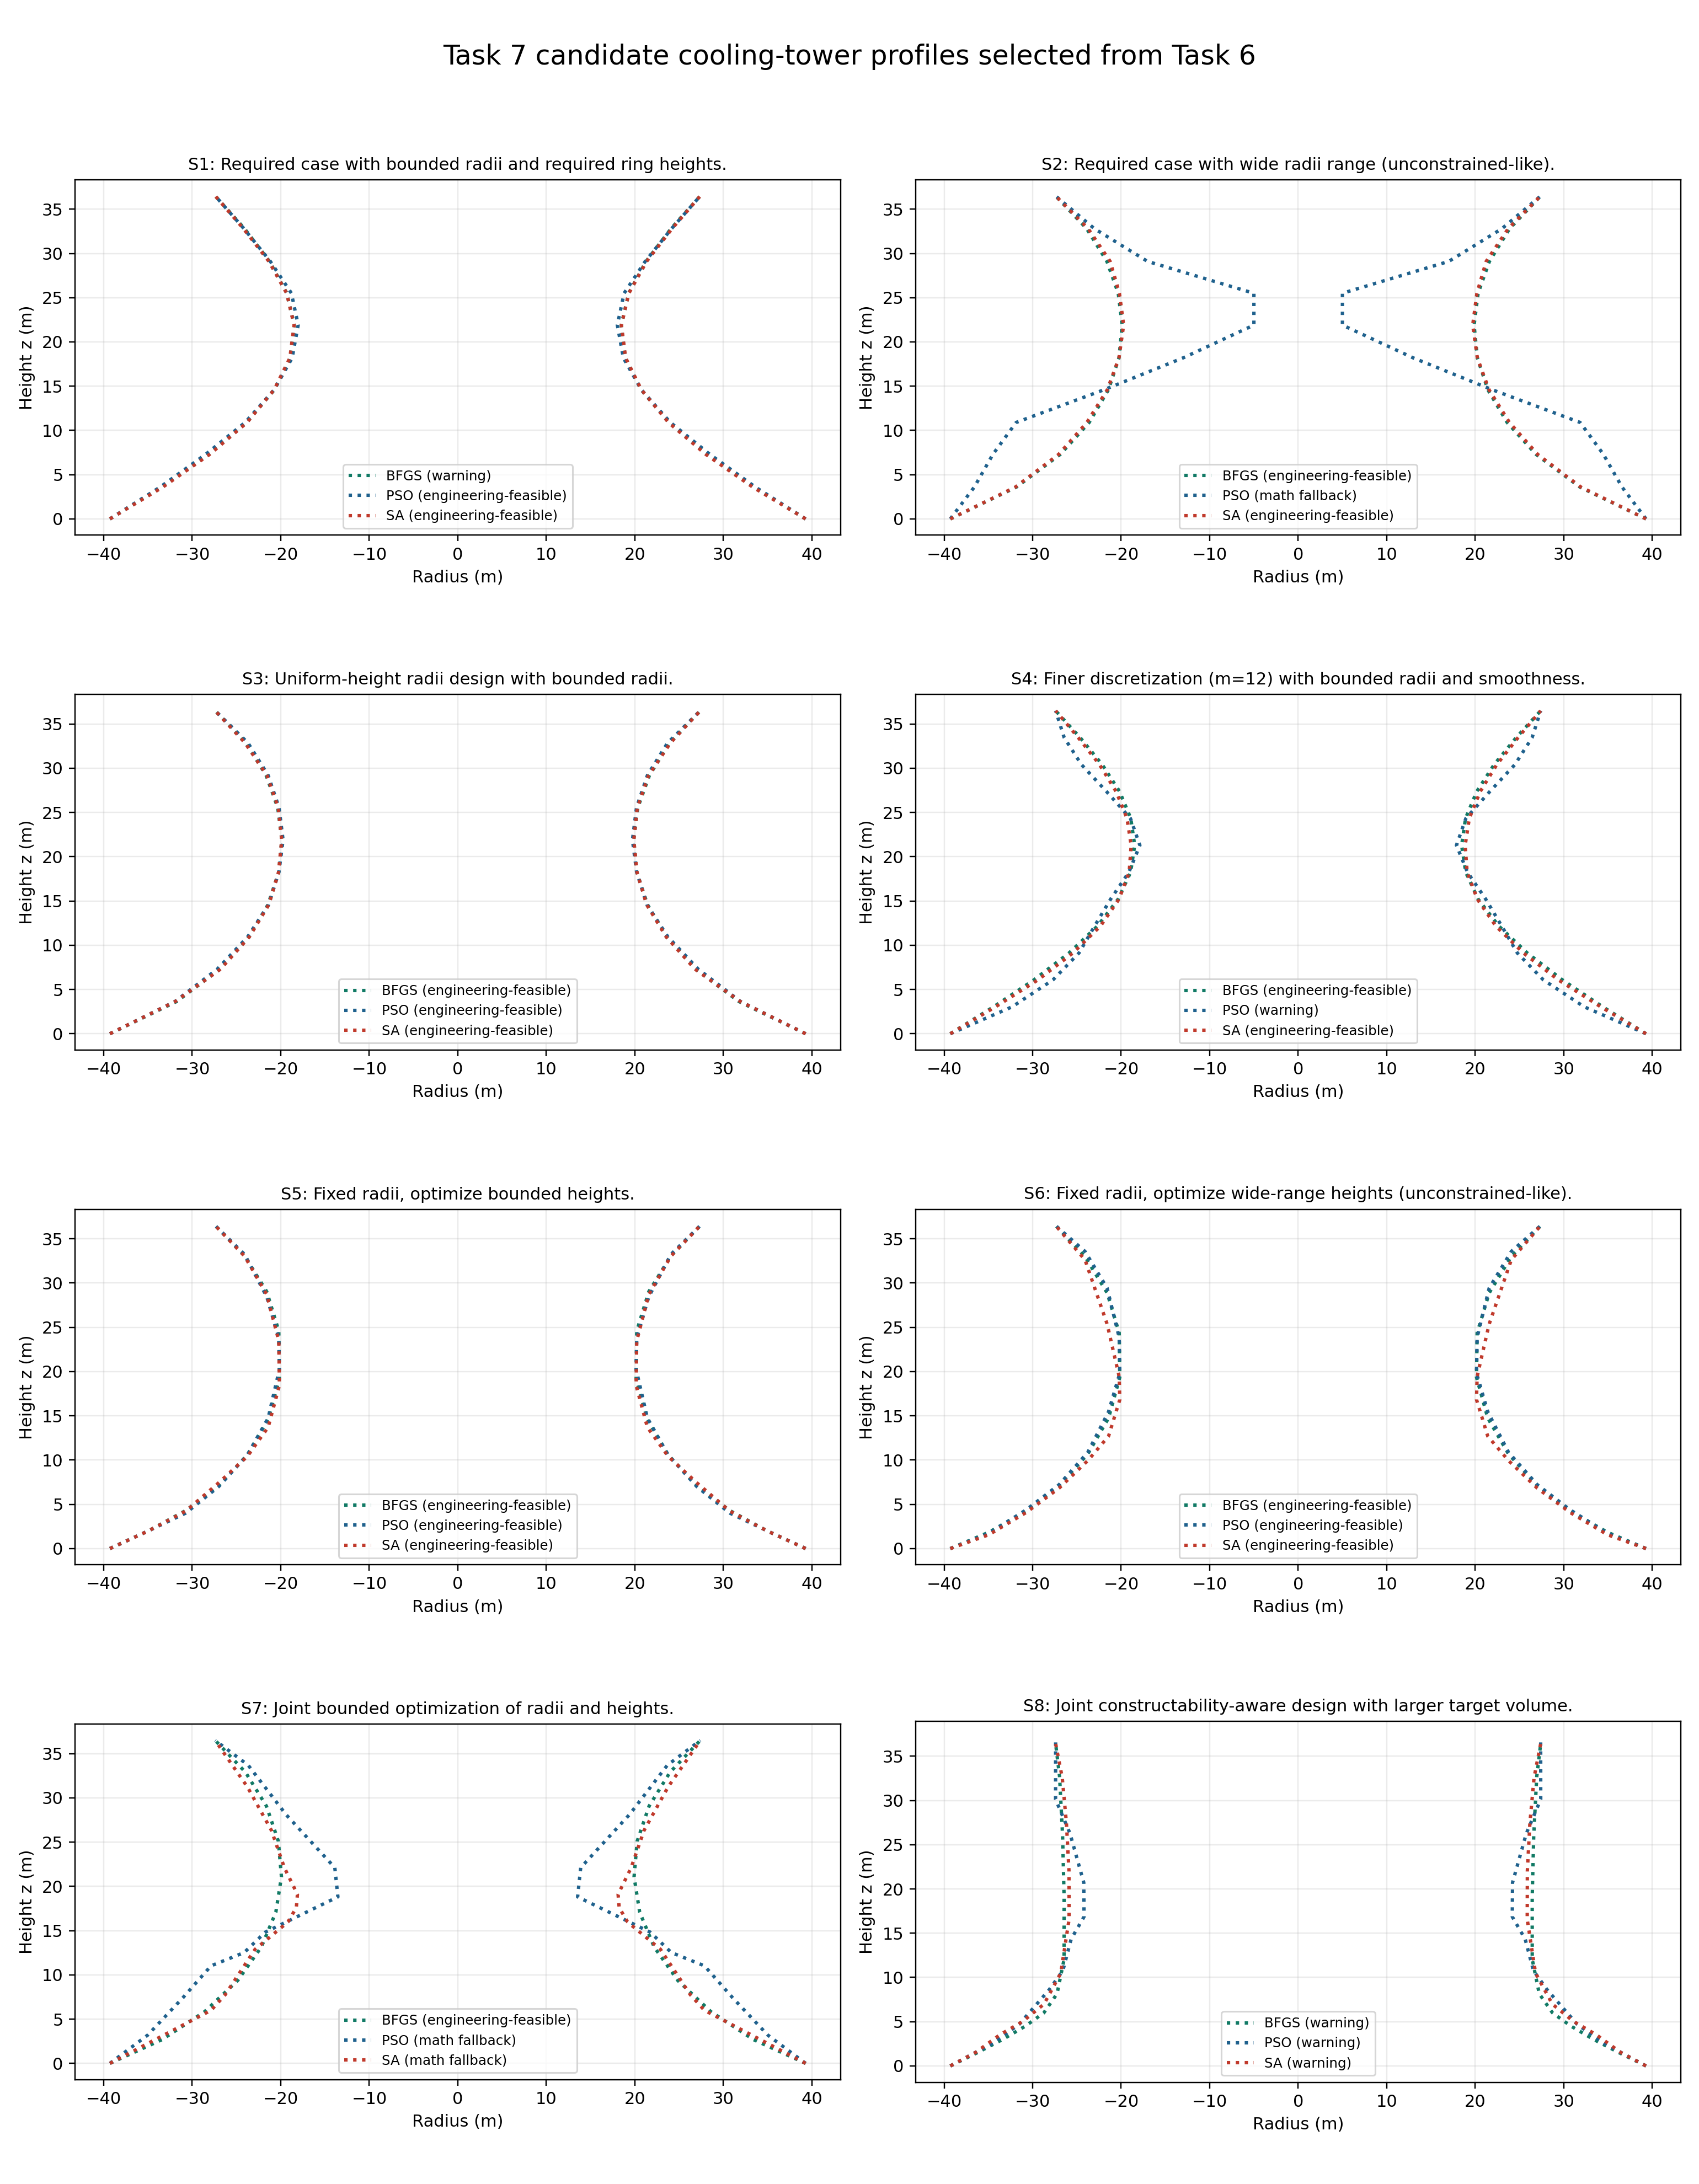
\includegraphics[width=0.95\textwidth]{../results/figures/candidate_profiles.png}
\caption{Task 7 candidate profiles}
\end{figure}


\chapter{3. Material, Loading, and CAE Setup}


\noindent Each model is built from the selected Task 6 meridian profile and revolved into a thin-shell cooling-tower surface; Task 7 keeps the exact Task 6 geometry scale.

\noindent The global coordinate convention is \texttt{Y}-up, with \texttt{X/Z} as the horizontal plane.

\noindent Material assumptions are uniform across all cases: equivalent reinforced concrete with \texttt{E = 33 GPa}, \texttt{nu = 0.20}, density \texttt{rho = 2500 kg/m³}, and shell thickness \texttt{t = 0.20 m}.

\noindent Loading combines self-weight and one-direction wind. The reference wind speed is \texttt{30.0 m/s}, giving \texttt{q = 562.5 Pa} from \(q = 0.5\,\rho_{air}V^2\).

\noindent Wind is modeled as external pressure on the shell with windward pressure and leeward suction (not internal cabin pressure). The circumferential pressure law is:

\[
C_p(\theta) = \mathrm{clip}(0.8\cos\theta, -0.5, 0.8), \quad p(\theta) = q\,C_p(\theta)
\]

\noindent Boundary conditions represent the tower support at the foundation/piler ring: base nodes are fixed (\texttt{U\_x = U\_y = U\_z = 0}), while the shell remains free elsewhere.

\noindent Each model uses one static step (\texttt{STATIC\_WIND}) for combined loading and one linear buckling step (\texttt{BUCKLING}) to extract the first instability modes about the preloaded state.


\chapter{4. Refined Structural Comparison Across All 24 Cases}


\begin{table}[H]
\centering
\scriptsize
\setlength{\tabcolsep}{4pt}
\renewcommand{\arraystretch}{1.1}
\resizebox{\textwidth}{!}{%
\begin{tabular}{@{}llllll@{}}
\hline
Case & Status & Task 6 area (m²) & Max disp. (mm) & Max stress (MPa) & Buckling factor \\
\hline
S1 / BFGS & Warning case & 7782.01 & 4.264 & 2.262 & 20.907 \\
S1 / PSO & Engineering-feasible & 7804.56 & 4.126 & 2.244 & 21.300 \\
S1 / SA & Engineering-feasible & 7780.73 & 4.627 & 2.368 & 21.481 \\
S2 / BFGS & Engineering-feasible & 7741.67 & 10.202 & 3.867 & 23.563 \\
S2 / PSO & Math fallback & 9075.03 & 94.040 & 10.268 & -3.229 \\
S2 / SA & Engineering-feasible & 7744.01 & 9.968 & 3.818 & 24.549 \\
S3 / BFGS & Engineering-feasible & 7741.69 & 10.153 & 3.834 & 23.529 \\
S3 / PSO & Engineering-feasible & 7743.34 & 9.850 & 3.794 & 23.496 \\
S3 / SA & Engineering-feasible & 7742.77 & 9.036 & 3.526 & 23.834 \\
S4 / BFGS & Engineering-feasible & 7779.85 & 3.831 & 2.282 & 20.267 \\
S4 / PSO & Warning case & 7931.66 & 12.073 & 4.541 & 22.491 \\
S4 / SA & Engineering-feasible & 7769.88 & 4.287 & 2.296 & 19.753 \\
S5 / BFGS & Engineering-feasible & 7742.56 & 8.695 & 4.148 & 22.725 \\
S5 / PSO & Engineering-feasible & 7747.93 & 11.481 & 4.941 & 19.566 \\
S5 / SA & Engineering-feasible & 7749.52 & 10.229 & 4.642 & 23.232 \\
S6 / BFGS & Engineering-feasible & 7741.72 & 10.522 & 5.312 & 24.772 \\
S6 / PSO & Engineering-feasible & 7748.25 & 11.907 & 6.705 & 21.611 \\
S6 / SA & Engineering-feasible & 7783.24 & 14.270 & 7.690 & 19.128 \\
S7 / BFGS & Engineering-feasible & 7740.66 & 10.105 & 4.134 & 24.948 \\
S7 / PSO & Math fallback & 8324.25 & 28.467 & 9.258 & 23.712 \\
S7 / SA & Math fallback & 7890.85 & 12.541 & 6.711 & 26.587 \\
S8 / BFGS & Warning case & 7813.24 & 10.319 & 5.446 & 19.273 \\
S8 / PSO & Warning case & 7899.07 & 9.235 & 4.493 & 27.335 \\
S8 / SA & Warning case & 7718.27 & 8.163 & 4.955 & 23.837 \\
\hline
\end{tabular}%
}
\end{table}


\begin{figure}[H]
\centering
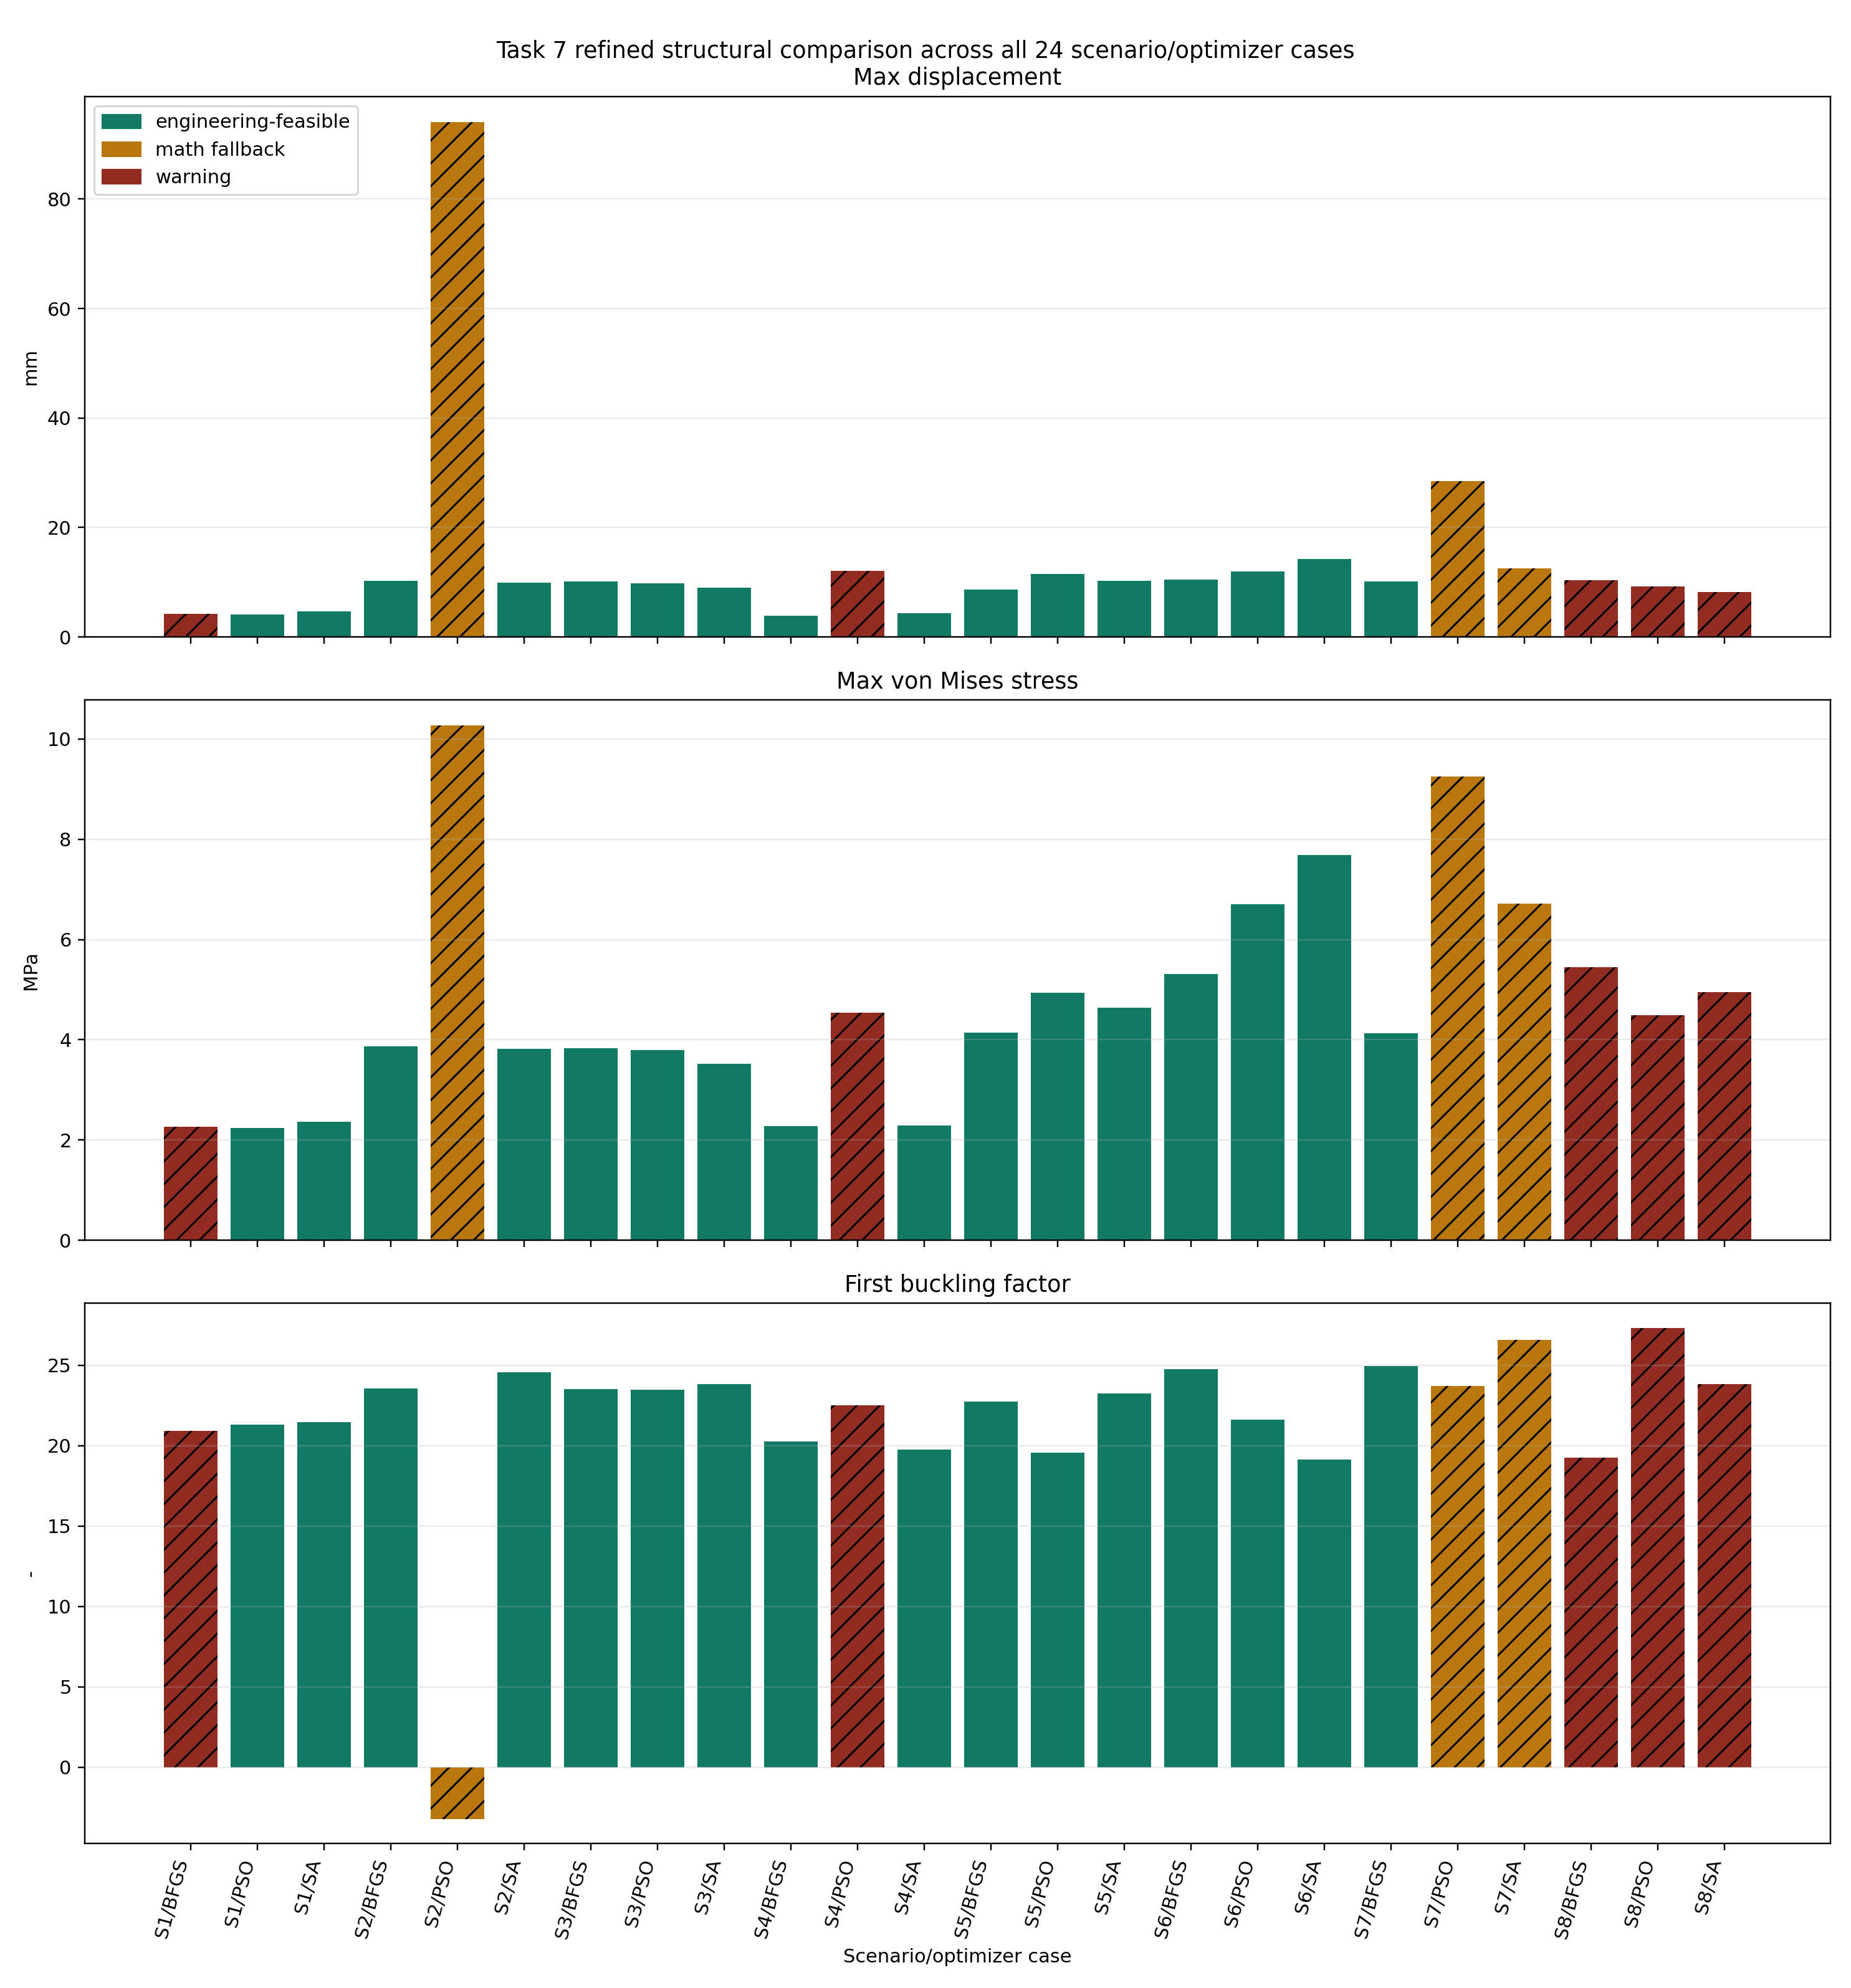
\includegraphics[width=0.95\textwidth]{../results/figures/comparison_metrics.png}
\caption{Task 7 refined comparison metrics}
\end{figure}


\noindent Figure 4.1 stacks displacement, stress, and buckling vertically to improve visibility and avoid compressed labels.

\noindent The first reading pass should prioritize buckling spread, then check whether displacement and stress trends confirm the same structural leader.


\chapter{5. Methodological Clarity and Global Ranking}


\section{5.1 Methodological Clarity}


\noindent The global ranking is a rank-based weighted score on the refined results, designed to stay robust when one or two cases have extreme values.

\noindent For each metric, rank \texttt{1} is best and rank \texttt{24} is worst, with deterministic tie-breaks by scenario/algorithm identifiers.


\[
r_i^{(k)} = \operatorname{rank}_k(i)
\]


\[
S_i = 0.45\,r_i^{(b)} + 0.25\,r_i^{(d)} + 0.20\,r_i^{(s)} + 0.10\,r_i^{(a)}
\]


\[
J_i = S_i + P_i, \quad P_i \in \{0,10,20\}
\]


\noindent Here \(r_i^{(b)}\) is the buckling rank (higher buckling is better), \(r_i^{(d)}\) is the displacement rank, \(r_i^{(s)}\) is the stress rank, and \(r_i^{(a)}\) is the area rank (lower is better for the last three).

\noindent Penalty points are \texttt{0} for engineering-feasible, \texttt{10} for mathematical fallback, and \texttt{20} for warning cases. The best model is the one with the lowest \texttt{J\_i}.


\section{5.2 Global Weighted Top-5}


\begin{table}[H]
\centering
\scriptsize
\setlength{\tabcolsep}{4pt}
\renewcommand{\arraystretch}{1.1}
\resizebox{\textwidth}{!}{%
\begin{tabular}{@{}lllllllll@{}}
\hline
Rank & Case & Status & Weighted score & Penalty & Buckling factor & Max disp. (mm) & Max stress (MPa) & Area (m²) \\
\hline
1 & S7 / BFGS & Engineering-feasible & 6.750 & 0.0 & 24.948 & 10.105 & 4.134 & 7740.66 \\
2 & S3 / SA & Engineering-feasible & 7.050 & 0.0 & 23.834 & 9.036 & 3.526 & 7742.77 \\
3 & S2 / SA & Engineering-feasible & 7.500 & 0.0 & 24.549 & 9.968 & 3.818 & 7744.01 \\
4 & S3 / PSO & Engineering-feasible & 9.650 & 0.0 & 23.496 & 9.850 & 3.794 & 7743.34 \\
5 & S2 / BFGS & Engineering-feasible & 9.850 & 0.0 & 23.563 & 10.202 & 3.867 & 7741.67 \\
\hline
\end{tabular}%
}
\end{table}


\begin{figure}[H]
\centering
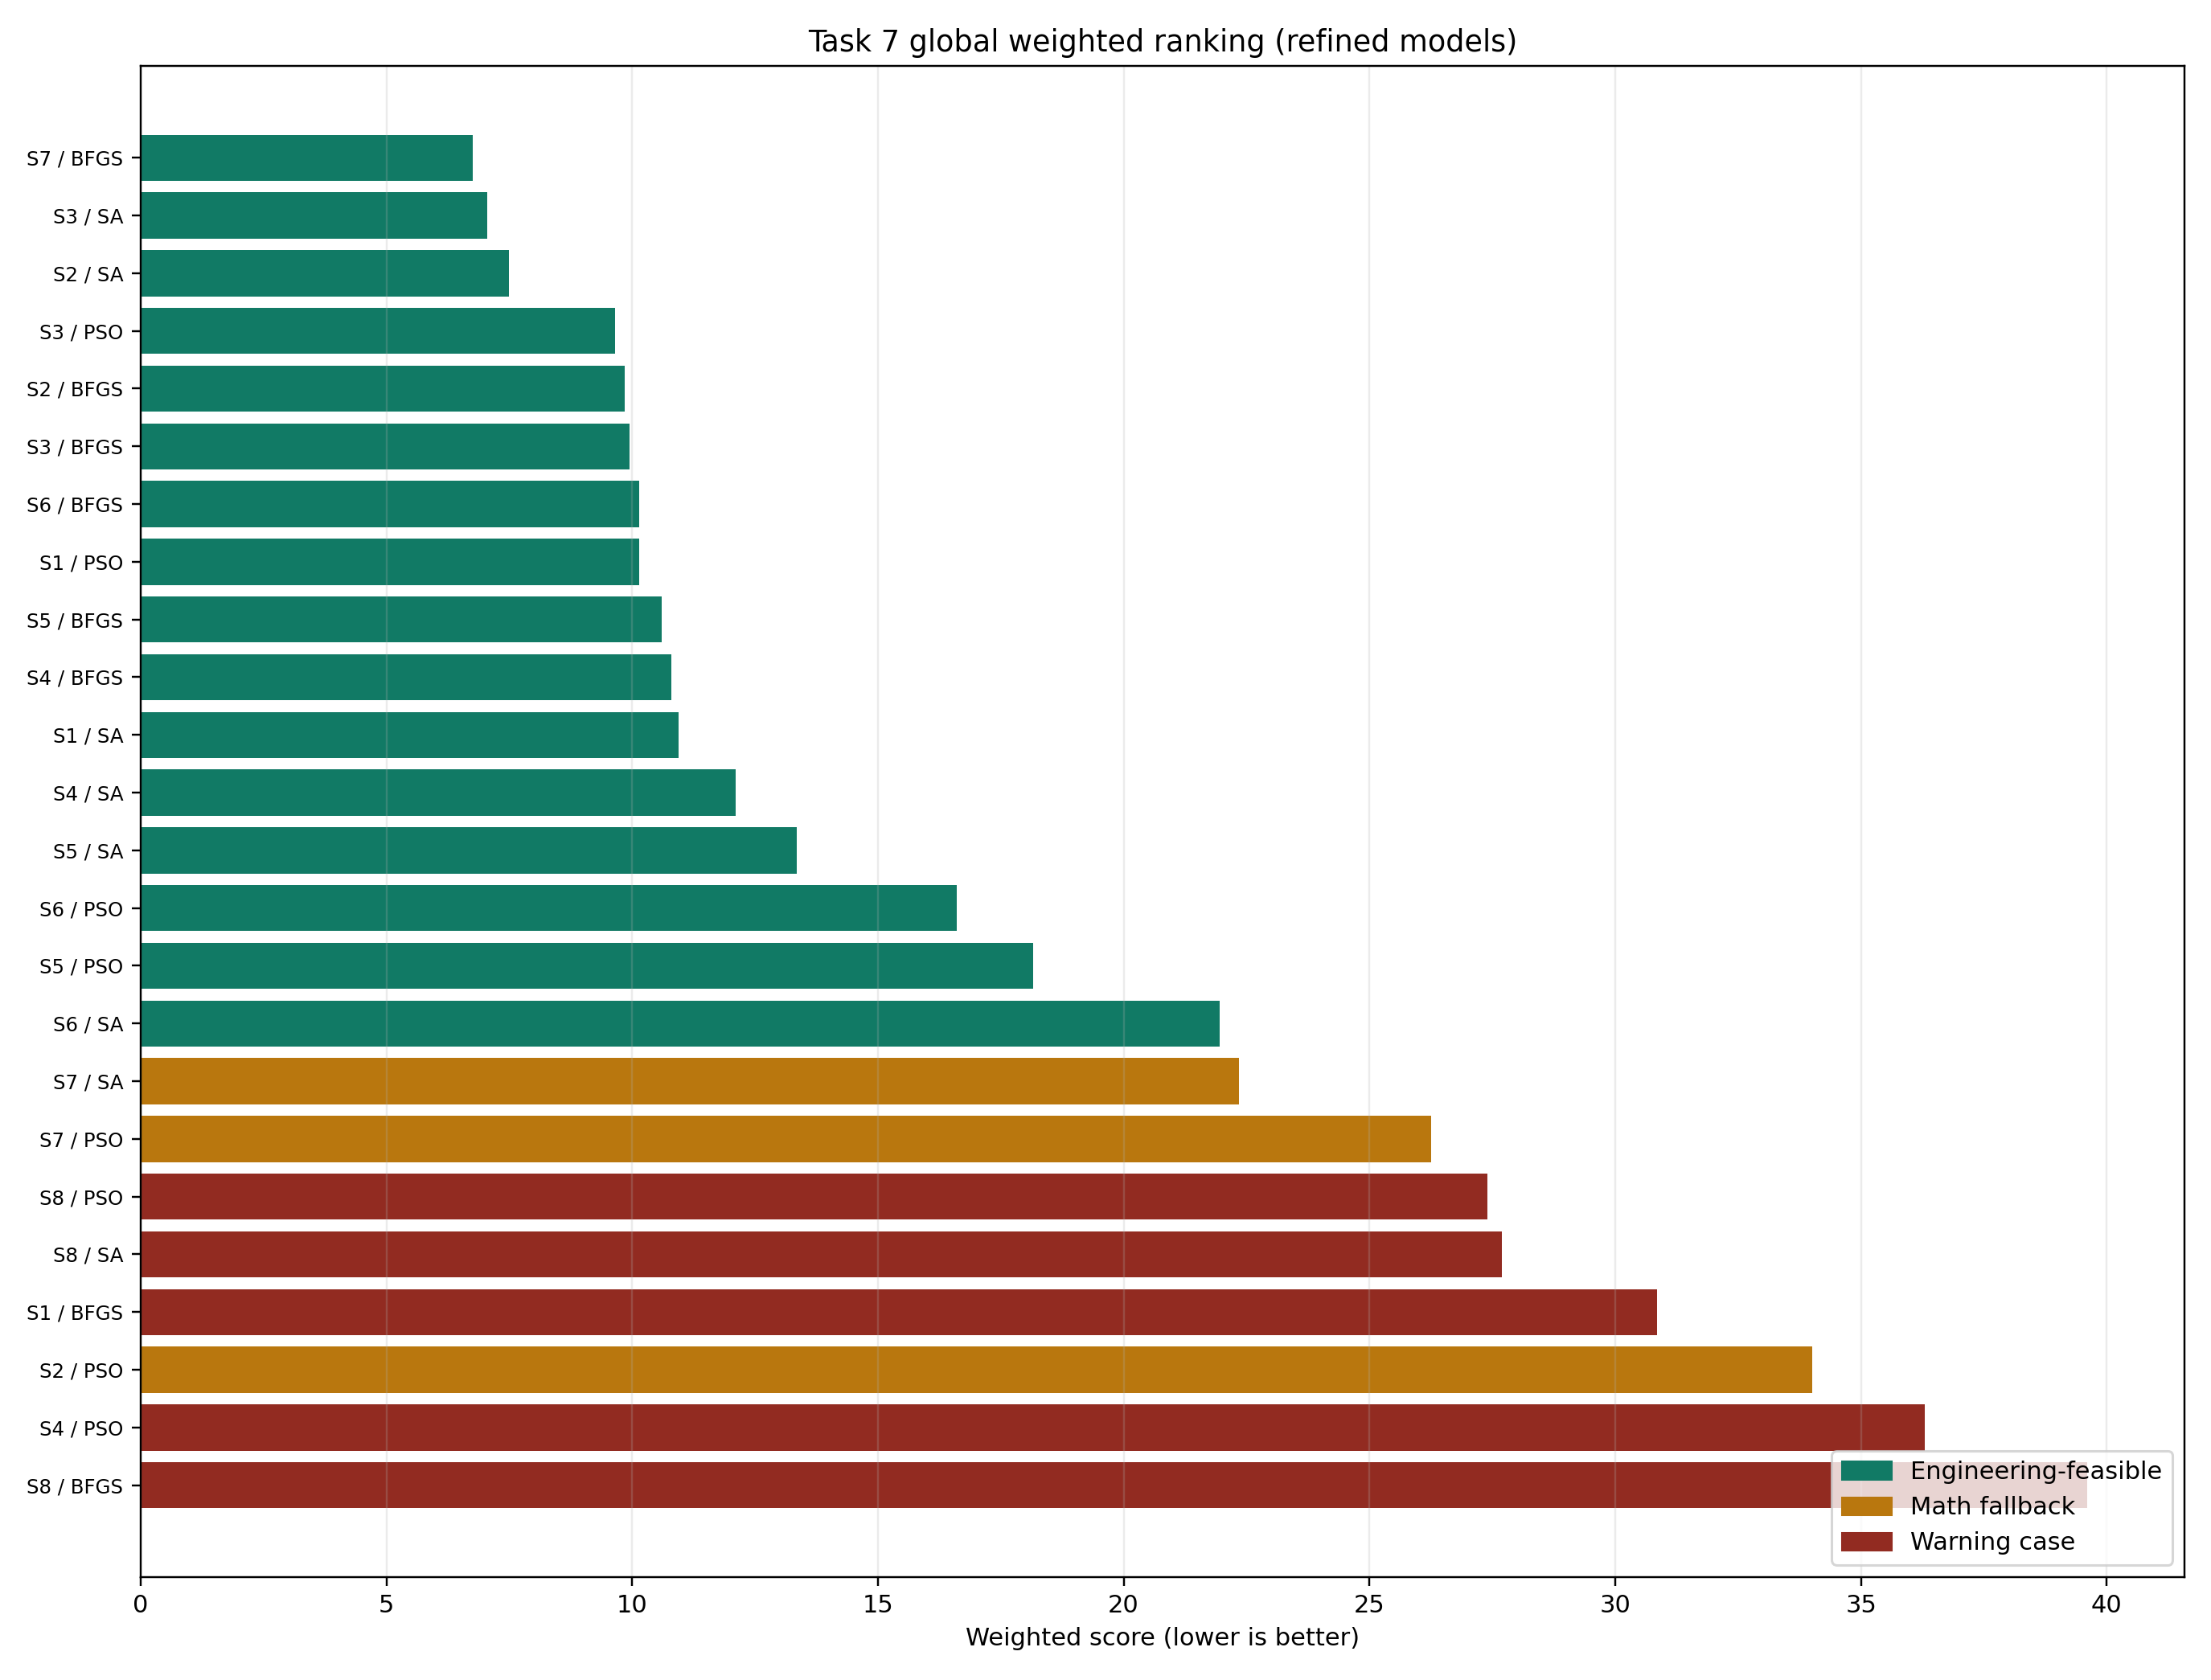
\includegraphics[width=0.95\textwidth]{../results/figures/task7_weighted_ranking.png}
\caption{Task 7 weighted ranking}
\end{figure}


\section{5.3 Top-3 by Criterion}


\subsection{5.3.1 Raw Top-3 (all statuses)}


\noindent This raw criterion table keeps all statuses visible, so warning and fallback cases can appear if they are numerically extreme on a single indicator.


\begin{table}[H]
\centering
\scriptsize
\setlength{\tabcolsep}{4pt}
\renewcommand{\arraystretch}{1.1}
\resizebox{\textwidth}{!}{%
\begin{tabular}{@{}lllll@{}}
\hline
Criterion & Rank & Case & Status & Value \\
\hline
Buckling factor & 1 & S8 / PSO & Warning case & 27.335 \\
Buckling factor & 2 & S7 / SA & Math fallback & 26.587 \\
Buckling factor & 3 & S7 / BFGS & Engineering-feasible & 24.948 \\
Max displacement & 1 & S4 / BFGS & Engineering-feasible & 3.831 mm \\
Max displacement & 2 & S1 / PSO & Engineering-feasible & 4.126 mm \\
Max displacement & 3 & S1 / BFGS & Warning case & 4.264 mm \\
Max stress & 1 & S1 / PSO & Engineering-feasible & 2.244 MPa \\
Max stress & 2 & S1 / BFGS & Warning case & 2.262 MPa \\
Max stress & 3 & S4 / BFGS & Engineering-feasible & 2.282 MPa \\
Task 6 area & 1 & S8 / SA & Warning case & 7718.27 m² \\
Task 6 area & 2 & S7 / BFGS & Engineering-feasible & 7740.66 m² \\
Task 6 area & 3 & S2 / BFGS & Engineering-feasible & 7741.67 m² \\
\hline
\end{tabular}%
}
\end{table}


\begin{figure}[H]
\centering
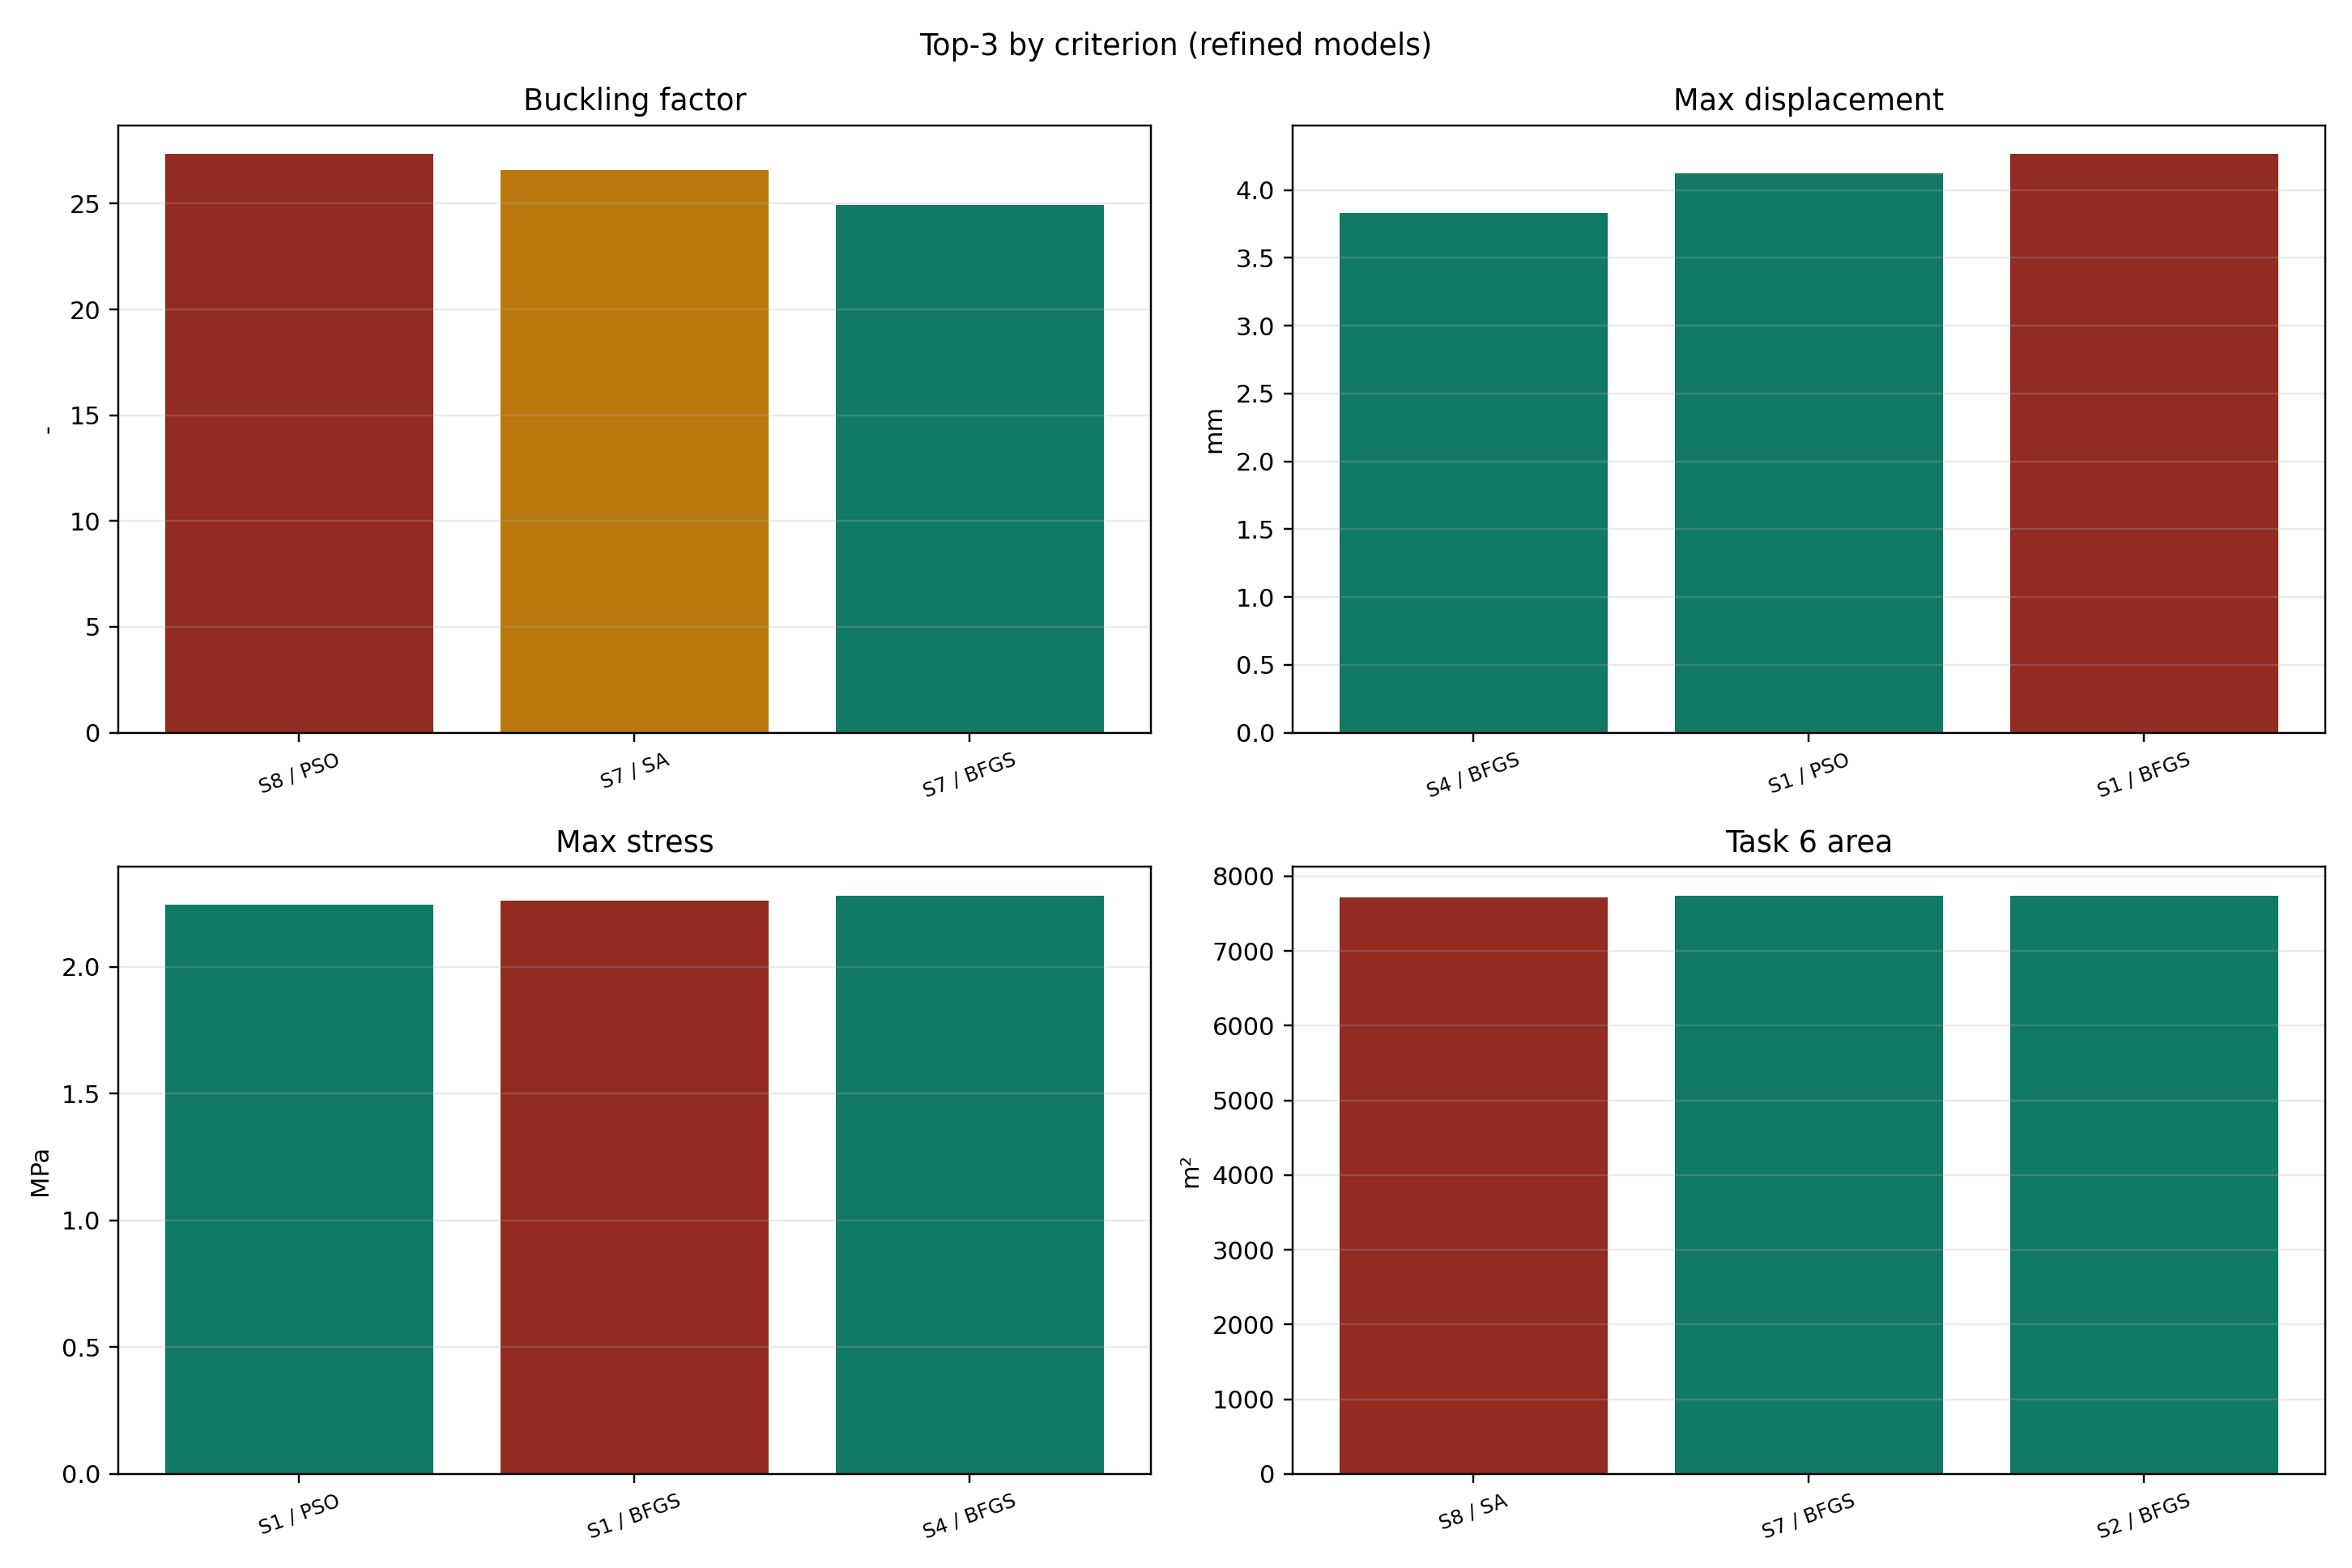
\includegraphics[width=0.95\textwidth]{../results/figures/task7_criterion_top3.png}
\caption{Task 7 criterion leaders}
\end{figure}


\subsection{5.3.2 Engineering-eligible Top-3}


\noindent This decision-grade table filters to engineering-feasible entries only.


\begin{table}[H]
\centering
\scriptsize
\setlength{\tabcolsep}{4pt}
\renewcommand{\arraystretch}{1.1}
\resizebox{\textwidth}{!}{%
\begin{tabular}{@{}lllll@{}}
\hline
Criterion & Rank & Case & Status & Value \\
\hline
Buckling factor & 1 & S7 / BFGS & Engineering-feasible & 24.948 \\
Buckling factor & 2 & S6 / BFGS & Engineering-feasible & 24.772 \\
Buckling factor & 3 & S2 / SA & Engineering-feasible & 24.549 \\
Max displacement & 1 & S4 / BFGS & Engineering-feasible & 3.831 mm \\
Max displacement & 2 & S1 / PSO & Engineering-feasible & 4.126 mm \\
Max displacement & 3 & S4 / SA & Engineering-feasible & 4.287 mm \\
Max stress & 1 & S1 / PSO & Engineering-feasible & 2.244 MPa \\
Max stress & 2 & S4 / BFGS & Engineering-feasible & 2.282 MPa \\
Max stress & 3 & S4 / SA & Engineering-feasible & 2.296 MPa \\
Task 6 area & 1 & S7 / BFGS & Engineering-feasible & 7740.66 m² \\
Task 6 area & 2 & S2 / BFGS & Engineering-feasible & 7741.67 m² \\
Task 6 area & 3 & S3 / BFGS & Engineering-feasible & 7741.69 m² \\
\hline
\end{tabular}%
}
\end{table}


\begin{figure}[H]
\centering
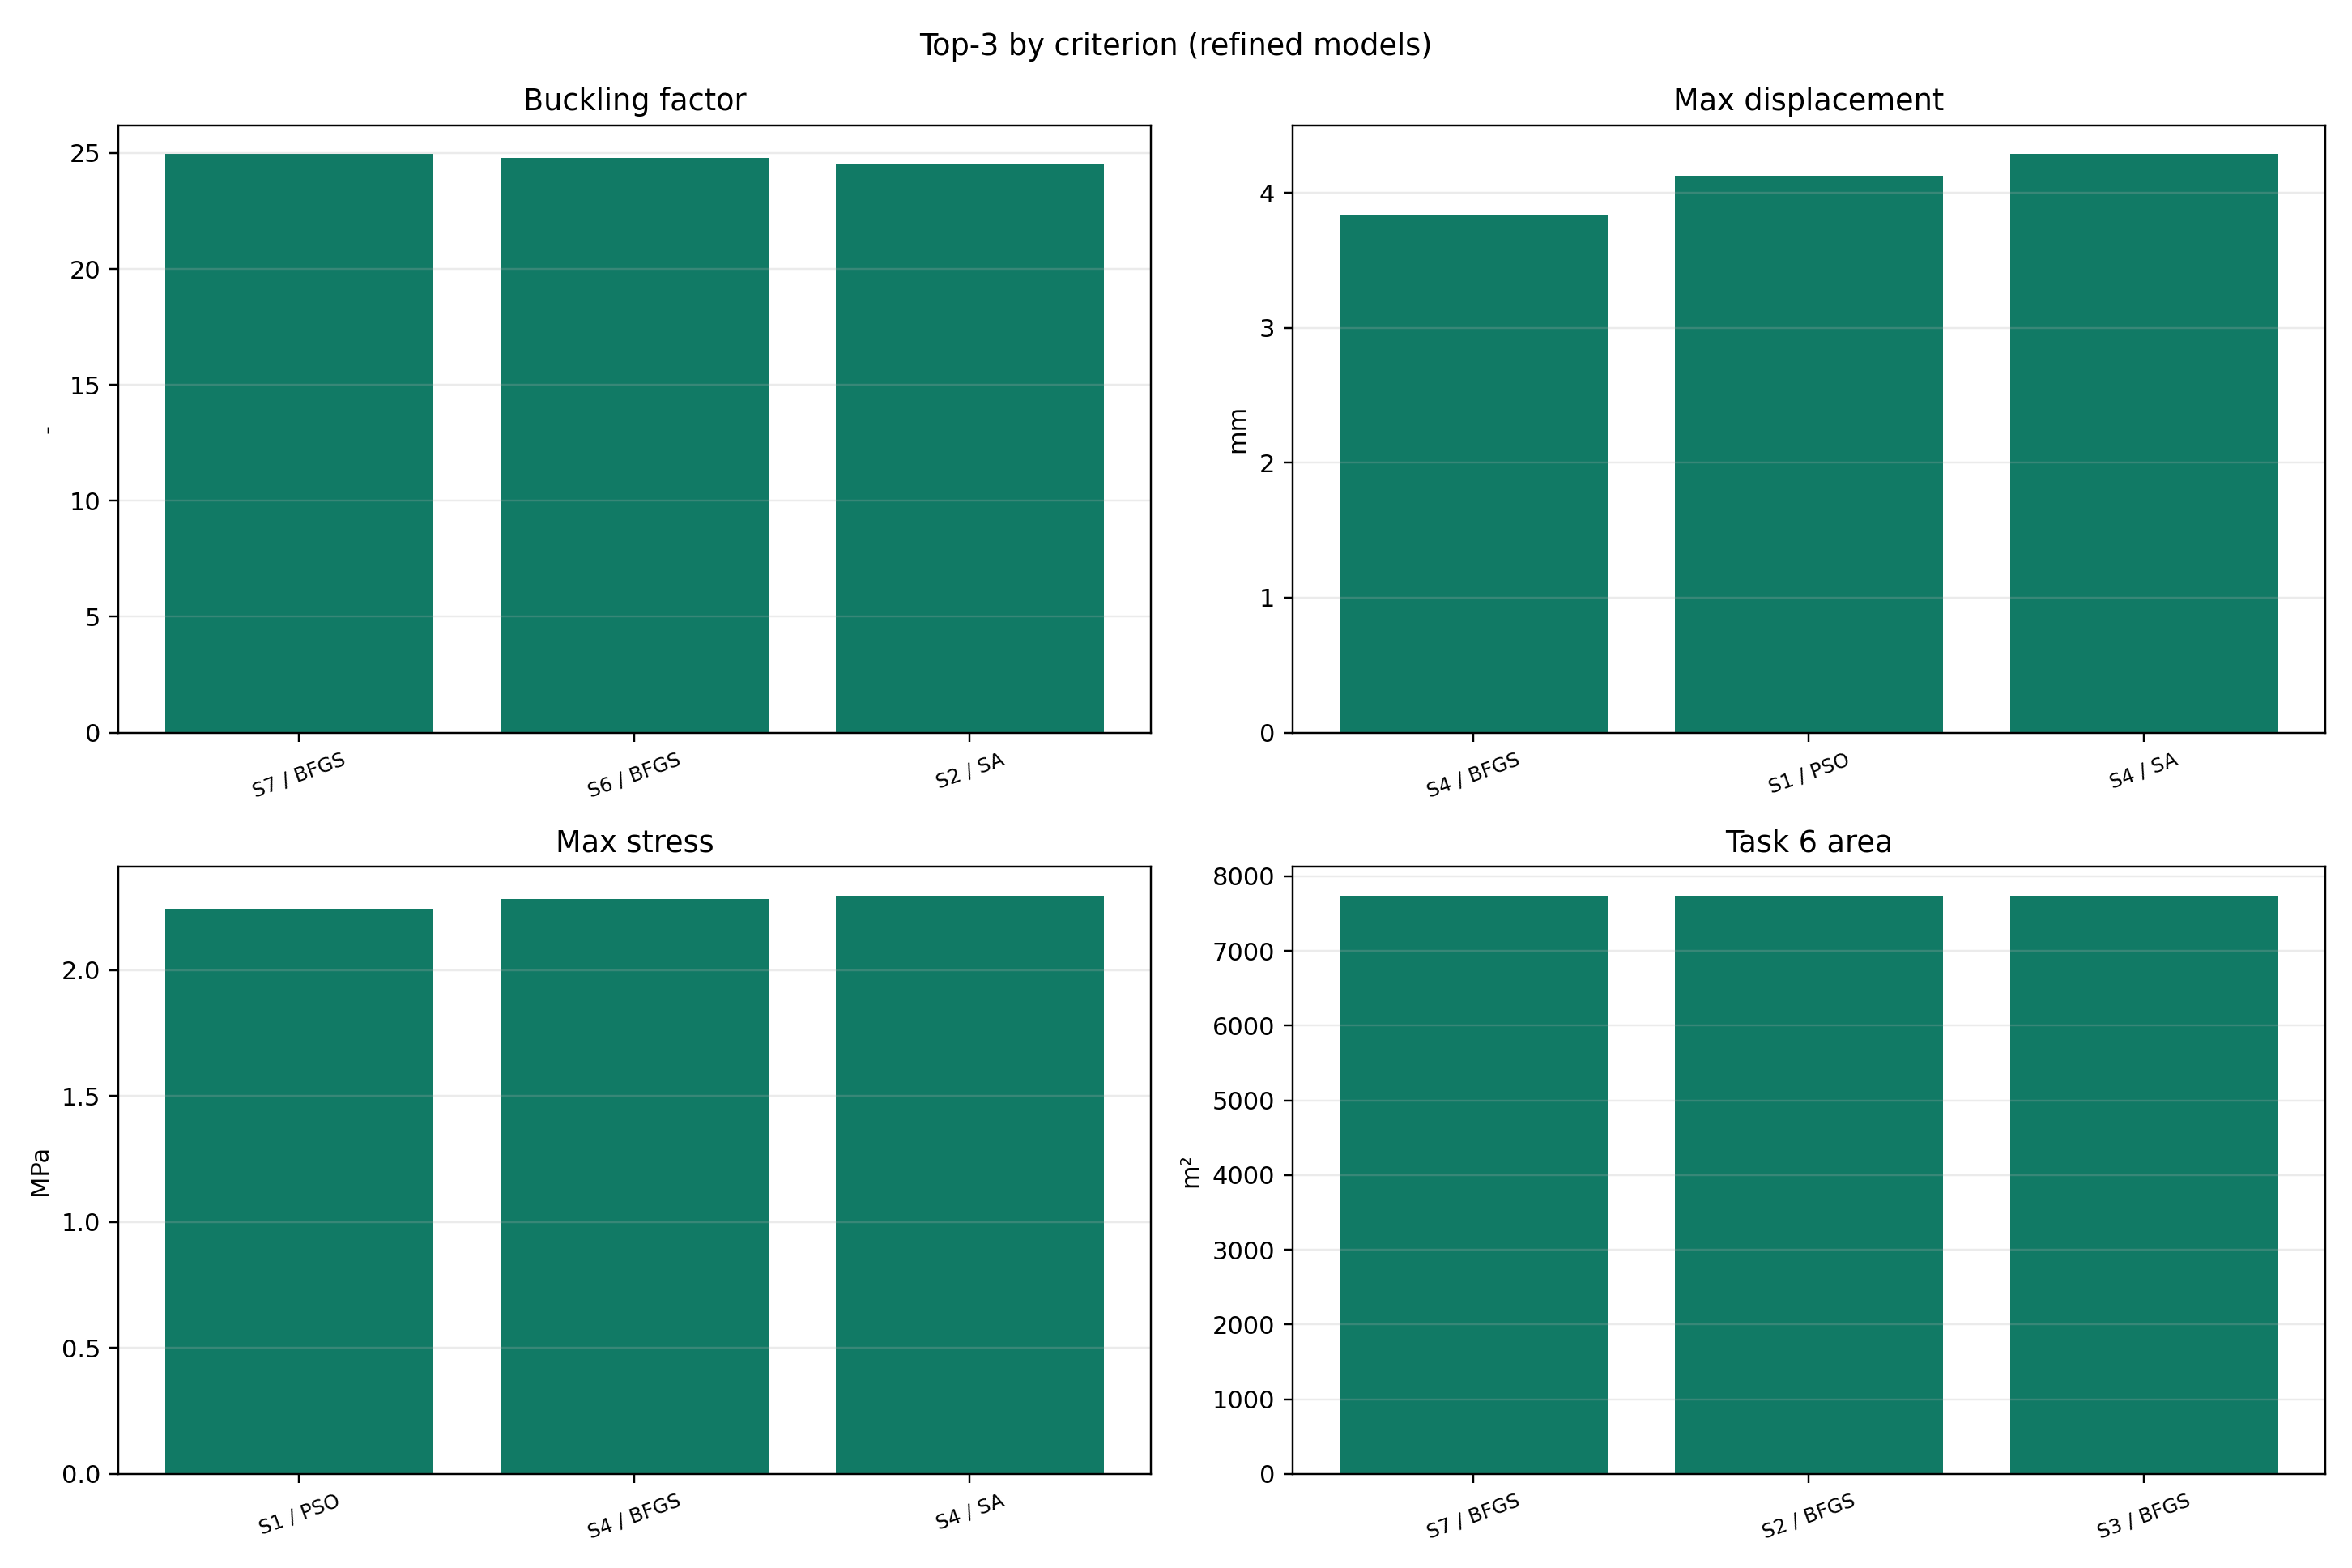
\includegraphics[width=0.95\textwidth]{../results/figures/task7_criterion_top3_engineering.png}
\caption{Task 7 engineering criterion leaders}
\end{figure}


\chapter{6. Scenario-by-Scenario Comparison}


\section{S1}


\begin{table}[H]
\centering
\scriptsize
\setlength{\tabcolsep}{4pt}
\renewcommand{\arraystretch}{1.1}
\resizebox{\textwidth}{!}{%
\begin{tabular}{@{}lllllll@{}}
\hline
Algorithm & Status & Weighted score & Task 6 area (m²) & Max disp. (mm) & Max stress (MPa) & Buckling factor \\
\hline
BFGS & Warning case & 30.850 & 7782.01 & 4.264 & 2.262 & 20.907 \\
PSO & Engineering-feasible & 10.150 & 7804.56 & 4.126 & 2.244 & 21.300 \\
SA & Engineering-feasible & 10.950 & 7780.73 & 4.627 & 2.368 & 21.481 \\
\hline
\end{tabular}%
}
\end{table}


\noindent \textbf{Winner:} S1 / PSO with weighted score \texttt{10.150}; gap to second place (S1 / SA) is \texttt{0.800}.

\noindent \textbf{Spread/Risk:} displacement spans \texttt{4.126} to \texttt{4.627} mm, stress spans \texttt{2.244} to \texttt{2.368} MPa, and buckling spans \texttt{20.907} to \texttt{21.481}.

\noindent \textbf{Status caveat:} warning-only entries are present for BFGS and are not decision-grade designs.

\noindent \textbf{Load dominance:} winner ratios are disp wind/gravity \texttt{0.107} and stress wind/gravity \texttt{0.073}; dominant drivers are displacement \texttt{gravity} and stress \texttt{gravity}.

\noindent \textbf{Critical note:} scenario fairness is reduced by mixed compliance statuses; ranking penalties keep the comparison visible but do not make warning/fallback cases equivalent to engineering-feasible designs.


\section{S2}


\begin{table}[H]
\centering
\scriptsize
\setlength{\tabcolsep}{4pt}
\renewcommand{\arraystretch}{1.1}
\resizebox{\textwidth}{!}{%
\begin{tabular}{@{}lllllll@{}}
\hline
Algorithm & Status & Weighted score & Task 6 area (m²) & Max disp. (mm) & Max stress (MPa) & Buckling factor \\
\hline
BFGS & Engineering-feasible & 9.850 & 7741.67 & 10.202 & 3.867 & 23.563 \\
PSO & Math fallback & 34.000 & 9075.03 & 94.040 & 10.268 & -3.229 \\
SA & Engineering-feasible & 7.500 & 7744.01 & 9.968 & 3.818 & 24.549 \\
\hline
\end{tabular}%
}
\end{table}


\noindent \textbf{Winner:} S2 / SA with weighted score \texttt{7.500}; gap to second place (S2 / BFGS) is \texttt{2.350}.

\noindent \textbf{Spread/Risk:} displacement spans \texttt{9.968} to \texttt{94.040} mm, stress spans \texttt{3.818} to \texttt{10.268} MPa, and buckling spans \texttt{-3.229} to \texttt{24.549}.

\noindent \textbf{Status caveat:} mathematical fallback entries are present for PSO.

\noindent \textbf{Load dominance:} winner ratios are disp wind/gravity \texttt{0.028} and stress wind/gravity \texttt{0.042}; dominant drivers are displacement \texttt{gravity} and stress \texttt{gravity}.

\noindent \textbf{Critical note:} scenario fairness is reduced by mixed compliance statuses; ranking penalties keep the comparison visible but do not make warning/fallback cases equivalent to engineering-feasible designs.


\section{S3}


\begin{table}[H]
\centering
\scriptsize
\setlength{\tabcolsep}{4pt}
\renewcommand{\arraystretch}{1.1}
\resizebox{\textwidth}{!}{%
\begin{tabular}{@{}lllllll@{}}
\hline
Algorithm & Status & Weighted score & Task 6 area (m²) & Max disp. (mm) & Max stress (MPa) & Buckling factor \\
\hline
BFGS & Engineering-feasible & 9.950 & 7741.69 & 10.153 & 3.834 & 23.529 \\
PSO & Engineering-feasible & 9.650 & 7743.34 & 9.850 & 3.794 & 23.496 \\
SA & Engineering-feasible & 7.050 & 7742.77 & 9.036 & 3.526 & 23.834 \\
\hline
\end{tabular}%
}
\end{table}


\noindent \textbf{Winner:} S3 / SA with weighted score \texttt{7.050}; gap to second place (S3 / PSO) is \texttt{2.600}.

\noindent \textbf{Spread/Risk:} displacement spans \texttt{9.036} to \texttt{10.153} mm, stress spans \texttt{3.526} to \texttt{3.834} MPa, and buckling spans \texttt{23.496} to \texttt{23.834}.

\noindent \textbf{Status caveat:} all three entries are engineering-feasible.

\noindent \textbf{Load dominance:} winner ratios are disp wind/gravity \texttt{0.034} and stress wind/gravity \texttt{0.049}; dominant drivers are displacement \texttt{gravity} and stress \texttt{gravity}.

\noindent \textbf{Critical note:} winner ranking is not yet convergence-locked on this scenario; keep this as screening guidance until mesh convergence is improved.


\section{S4}


\begin{table}[H]
\centering
\scriptsize
\setlength{\tabcolsep}{4pt}
\renewcommand{\arraystretch}{1.1}
\resizebox{\textwidth}{!}{%
\begin{tabular}{@{}lllllll@{}}
\hline
Algorithm & Status & Weighted score & Task 6 area (m²) & Max disp. (mm) & Max stress (MPa) & Buckling factor \\
\hline
BFGS & Engineering-feasible & 10.800 & 7779.85 & 3.831 & 2.282 & 20.267 \\
PSO & Warning case & 36.300 & 7931.66 & 12.073 & 4.541 & 22.491 \\
SA & Engineering-feasible & 12.100 & 7769.88 & 4.287 & 2.296 & 19.753 \\
\hline
\end{tabular}%
}
\end{table}


\noindent \textbf{Winner:} S4 / BFGS with weighted score \texttt{10.800}; gap to second place (S4 / SA) is \texttt{1.300}.

\noindent \textbf{Spread/Risk:} displacement spans \texttt{3.831} to \texttt{12.073} mm, stress spans \texttt{2.282} to \texttt{4.541} MPa, and buckling spans \texttt{19.753} to \texttt{22.491}.

\noindent \textbf{Status caveat:} warning-only entries are present for PSO and are not decision-grade designs.

\noindent \textbf{Load dominance:} winner ratios are disp wind/gravity \texttt{0.078} and stress wind/gravity \texttt{0.079}; dominant drivers are displacement \texttt{gravity} and stress \texttt{gravity}.

\noindent \textbf{Critical note:} scenario fairness is reduced by mixed compliance statuses; ranking penalties keep the comparison visible but do not make warning/fallback cases equivalent to engineering-feasible designs.


\section{S5}


\begin{table}[H]
\centering
\scriptsize
\setlength{\tabcolsep}{4pt}
\renewcommand{\arraystretch}{1.1}
\resizebox{\textwidth}{!}{%
\begin{tabular}{@{}lllllll@{}}
\hline
Algorithm & Status & Weighted score & Task 6 area (m²) & Max disp. (mm) & Max stress (MPa) & Buckling factor \\
\hline
BFGS & Engineering-feasible & 10.600 & 7742.56 & 8.695 & 4.148 & 22.725 \\
PSO & Engineering-feasible & 18.150 & 7747.93 & 11.481 & 4.941 & 19.566 \\
SA & Engineering-feasible & 13.350 & 7749.52 & 10.229 & 4.642 & 23.232 \\
\hline
\end{tabular}%
}
\end{table}


\noindent \textbf{Winner:} S5 / BFGS with weighted score \texttt{10.600}; gap to second place (S5 / SA) is \texttt{2.750}.

\noindent \textbf{Spread/Risk:} displacement spans \texttt{8.695} to \texttt{11.481} mm, stress spans \texttt{4.148} to \texttt{4.941} MPa, and buckling spans \texttt{19.566} to \texttt{23.232}.

\noindent \textbf{Status caveat:} all three entries are engineering-feasible.

\noindent \textbf{Load dominance:} winner ratios are disp wind/gravity \texttt{0.034} and stress wind/gravity \texttt{0.044}; dominant drivers are displacement \texttt{gravity} and stress \texttt{gravity}.

\noindent \textbf{Critical note:} winner ranking is not yet convergence-locked on this scenario; keep this as screening guidance until mesh convergence is improved.


\section{S6}


\begin{table}[H]
\centering
\scriptsize
\setlength{\tabcolsep}{4pt}
\renewcommand{\arraystretch}{1.1}
\resizebox{\textwidth}{!}{%
\begin{tabular}{@{}lllllll@{}}
\hline
Algorithm & Status & Weighted score & Task 6 area (m²) & Max disp. (mm) & Max stress (MPa) & Buckling factor \\
\hline
BFGS & Engineering-feasible & 10.150 & 7741.72 & 10.522 & 5.312 & 24.772 \\
PSO & Engineering-feasible & 16.600 & 7748.25 & 11.907 & 6.705 & 21.611 \\
SA & Engineering-feasible & 21.950 & 7783.24 & 14.270 & 7.690 & 19.128 \\
\hline
\end{tabular}%
}
\end{table}


\noindent \textbf{Winner:} S6 / BFGS with weighted score \texttt{10.150}; gap to second place (S6 / PSO) is \texttt{6.450}.

\noindent \textbf{Spread/Risk:} displacement spans \texttt{10.522} to \texttt{14.270} mm, stress spans \texttt{5.312} to \texttt{7.690} MPa, and buckling spans \texttt{19.128} to \texttt{24.772}.

\noindent \textbf{Status caveat:} all three entries are engineering-feasible.

\noindent \textbf{Load dominance:} winner ratios are disp wind/gravity \texttt{0.026} and stress wind/gravity \texttt{0.030}; dominant drivers are displacement \texttt{gravity} and stress \texttt{gravity}.

\noindent \textbf{Critical note:} winner ranking is not yet convergence-locked on this scenario; keep this as screening guidance until mesh convergence is improved.


\section{S7}


\begin{table}[H]
\centering
\scriptsize
\setlength{\tabcolsep}{4pt}
\renewcommand{\arraystretch}{1.1}
\resizebox{\textwidth}{!}{%
\begin{tabular}{@{}lllllll@{}}
\hline
Algorithm & Status & Weighted score & Task 6 area (m²) & Max disp. (mm) & Max stress (MPa) & Buckling factor \\
\hline
BFGS & Engineering-feasible & 6.750 & 7740.66 & 10.105 & 4.134 & 24.948 \\
PSO & Math fallback & 26.250 & 8324.25 & 28.467 & 9.258 & 23.712 \\
SA & Math fallback & 22.350 & 7890.85 & 12.541 & 6.711 & 26.587 \\
\hline
\end{tabular}%
}
\end{table}


\noindent \textbf{Winner:} S7 / BFGS with weighted score \texttt{6.750}; gap to second place (S7 / SA) is \texttt{15.600}.

\noindent \textbf{Spread/Risk:} displacement spans \texttt{10.105} to \texttt{28.467} mm, stress spans \texttt{4.134} to \texttt{9.258} MPa, and buckling spans \texttt{23.712} to \texttt{26.587}.

\noindent \textbf{Status caveat:} mathematical fallback entries are present for PSO, SA.

\noindent \textbf{Load dominance:} winner ratios are disp wind/gravity \texttt{0.029} and stress wind/gravity \texttt{0.036}; dominant drivers are displacement \texttt{gravity} and stress \texttt{gravity}.

\noindent \textbf{Critical note:} scenario fairness is reduced by mixed compliance statuses; ranking penalties keep the comparison visible but do not make warning/fallback cases equivalent to engineering-feasible designs.


\section{S8}


\begin{table}[H]
\centering
\scriptsize
\setlength{\tabcolsep}{4pt}
\renewcommand{\arraystretch}{1.1}
\resizebox{\textwidth}{!}{%
\begin{tabular}{@{}lllllll@{}}
\hline
Algorithm & Status & Weighted score & Task 6 area (m²) & Max disp. (mm) & Max stress (MPa) & Buckling factor \\
\hline
BFGS & Warning case & 39.600 & 7813.24 & 10.319 & 5.446 & 19.273 \\
PSO & Warning case & 27.400 & 7899.07 & 9.235 & 4.493 & 27.335 \\
SA & Warning case & 27.700 & 7718.27 & 8.163 & 4.955 & 23.837 \\
\hline
\end{tabular}%
}
\end{table}


\noindent \textbf{Winner:} S8 / PSO with weighted score \texttt{27.400}; gap to second place (S8 / SA) is \texttt{0.300}.

\noindent \textbf{Spread/Risk:} displacement spans \texttt{8.163} to \texttt{10.319} mm, stress spans \texttt{4.493} to \texttt{5.446} MPa, and buckling spans \texttt{19.273} to \texttt{27.335}.

\noindent \textbf{Status caveat:} warning-only entries are present for BFGS, PSO, SA and are not decision-grade designs.

\noindent \textbf{Load dominance:} winner ratios are disp wind/gravity \texttt{0.069} and stress wind/gravity \texttt{0.041}; dominant drivers are displacement \texttt{gravity} and stress \texttt{gravity}.

\noindent \textbf{Critical note:} winner ranking is not yet convergence-locked on this scenario; keep this as screening guidance until mesh convergence is improved.


\chapter{7. Convergence Summary}


\noindent The verification workflow solves both coarse and refined meshes for every case. The acceptance criteria are: displacement change below \texttt{5.0\%}, stress change below \texttt{5.0\%}, and first buckling-factor change below \texttt{10.0\%}.


\noindent At the current stage, \textbf{0 of 24 comparison pairs} satisfy all three convergence criteria.

\noindent Because the study is currently at \texttt{0/24} all-pass convergence, the ranking should be interpreted as comparative screening quality, not final structural qualification.


\begin{table}[H]
\centering
\scriptsize
\setlength{\tabcolsep}{4pt}
\renewcommand{\arraystretch}{1.1}
\resizebox{\textwidth}{!}{%
\begin{tabular}{@{}lllllllll@{}}
\hline
Case & Status & Delta disp. (\%) & Pass & Delta stress (\%) & Pass & Delta buckling (\%) & Pass & All pass \\
\hline
S1 / BFGS & Warning case & 8.66 & no & 3.95 & yes & -51.38 & no & no \\
S1 / PSO & Engineering-feasible & 17.03 & no & 8.32 & no & -51.39 & no & no \\
S1 / SA & Engineering-feasible & 9.59 & no & 2.24 & yes & -49.67 & no & no \\
S2 / BFGS & Engineering-feasible & 27.17 & no & 0.60 & yes & -48.05 & no & no \\
S2 / PSO & Math fallback & -11.47 & no & -60.11 & no & -5.64 & yes & no \\
S2 / SA & Engineering-feasible & 25.49 & no & -1.19 & yes & -46.75 & no & no \\
S3 / BFGS & Engineering-feasible & 26.57 & no & -0.73 & yes & -48.06 & no & no \\
S3 / PSO & Engineering-feasible & 27.31 & no & 1.44 & yes & -50.01 & no & no \\
S3 / SA & Engineering-feasible & 21.16 & no & -3.57 & yes & -46.37 & no & no \\
S4 / BFGS & Engineering-feasible & -5.76 & no & 7.01 & no & -51.16 & no & no \\
S4 / PSO & Warning case & 16.53 & no & -3.15 & yes & -158.30 & no & no \\
S4 / SA & Engineering-feasible & -7.69 & no & 1.43 & yes & -49.02 & no & no \\
S5 / BFGS & Engineering-feasible & -5.89 & no & 10.45 & no & -46.31 & no & no \\
S5 / PSO & Engineering-feasible & 1.17 & yes & 23.43 & no & -49.25 & no & no \\
S5 / SA & Engineering-feasible & -2.76 & yes & 5.00 & no & -45.85 & no & no \\
S6 / BFGS & Engineering-feasible & 2.08 & yes & 20.49 & no & -41.81 & no & no \\
S6 / PSO & Engineering-feasible & 17.42 & no & 39.74 & no & -54.85 & no & no \\
S6 / SA & Engineering-feasible & 15.36 & no & 38.65 & no & -55.49 & no & no \\
S7 / BFGS & Engineering-feasible & 17.31 & no & 0.69 & yes & -43.58 & no & no \\
S7 / PSO & Math fallback & 11.87 & no & -19.73 & no & -240.70 & no & no \\
S7 / SA & Math fallback & -6.17 & no & -19.68 & no & -63.19 & no & no \\
S8 / BFGS & Warning case & 2.71 & yes & 10.91 & no & -53.42 & no & no \\
S8 / PSO & Warning case & 7.91 & no & -0.58 & yes & -49.86 & no & no \\
S8 / SA & Warning case & 5.04 & no & 15.88 & no & -53.02 & no & no \\
\hline
\end{tabular}%
}
\end{table}


\begin{figure}[H]
\centering
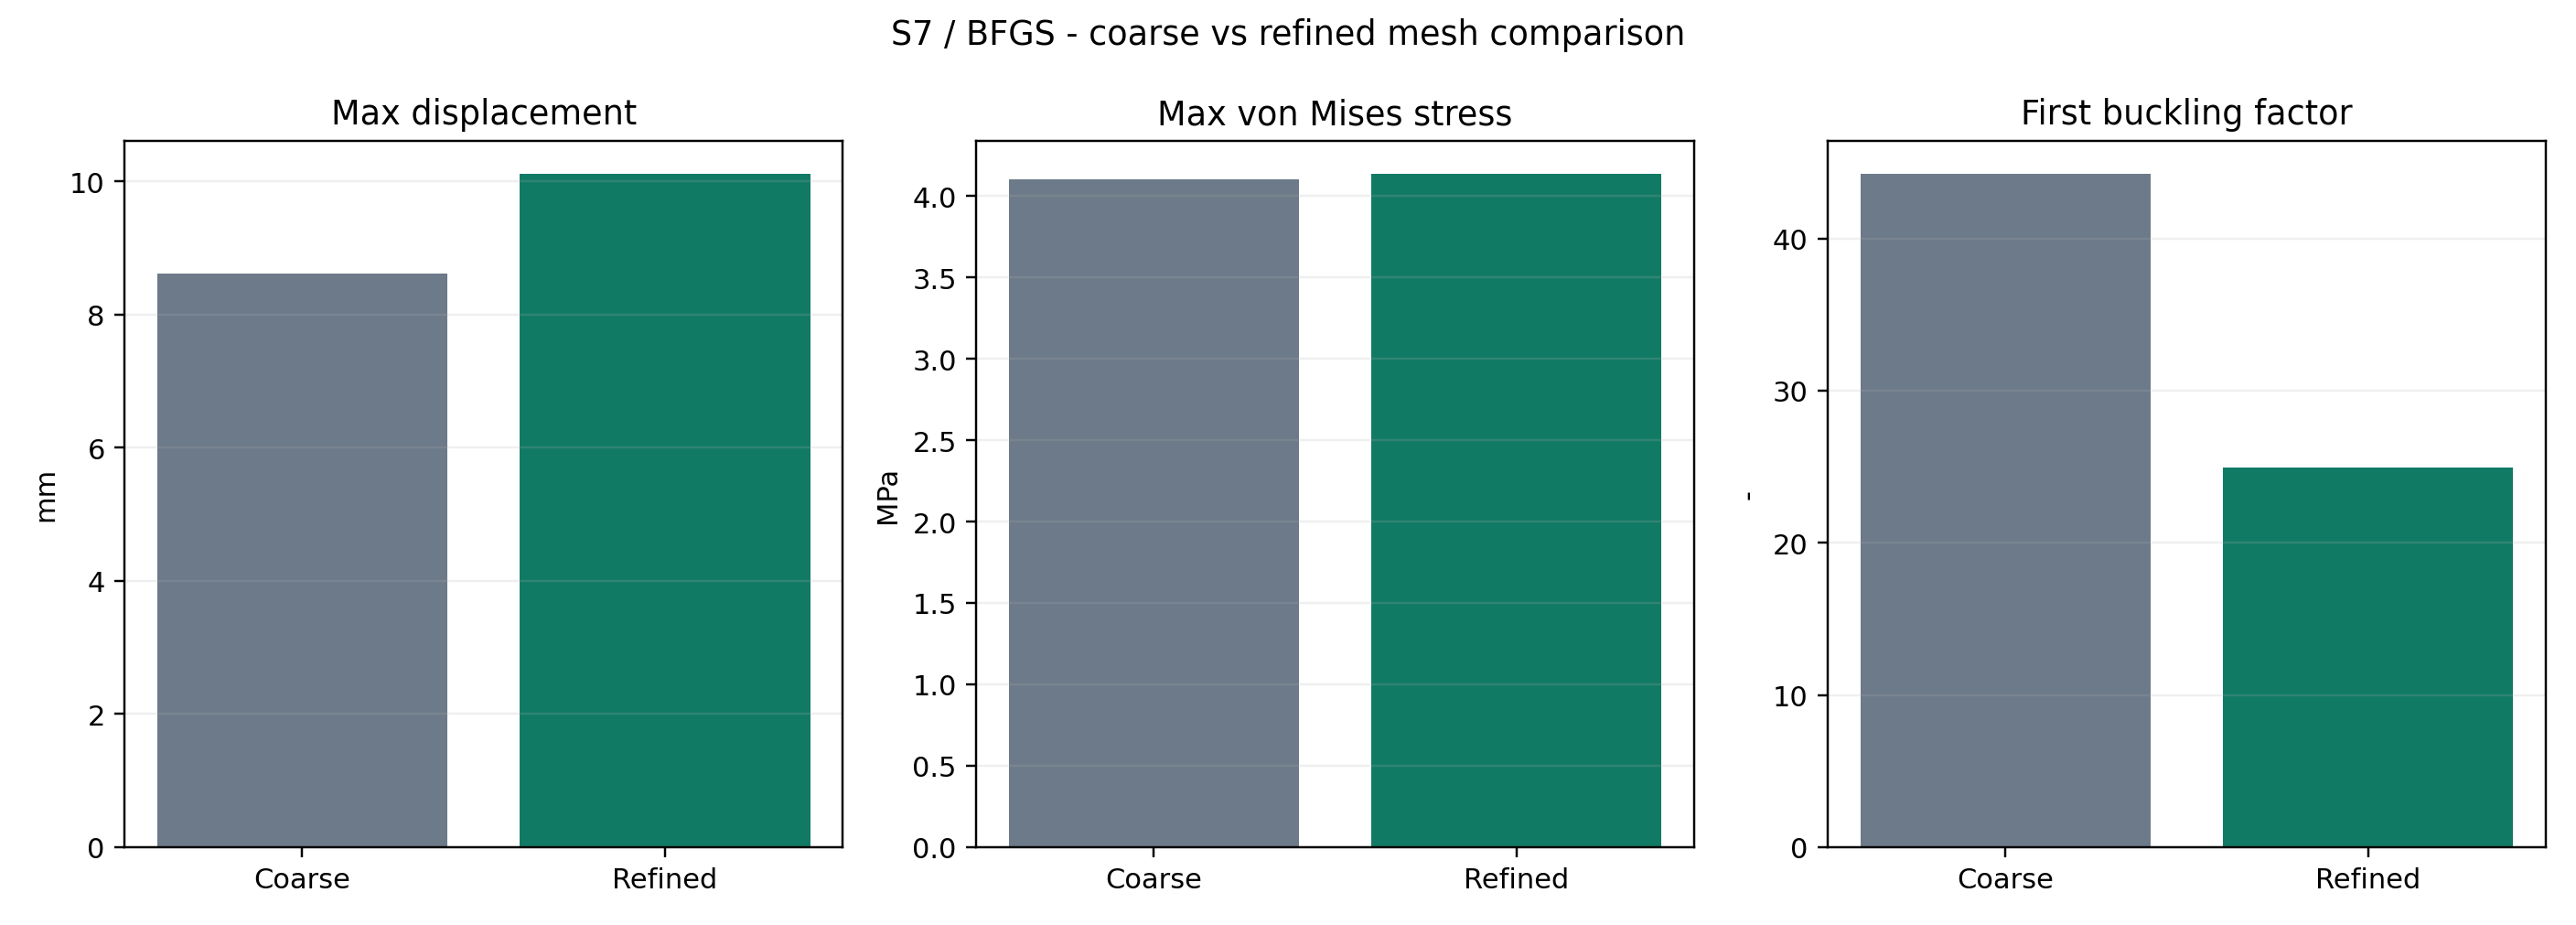
\includegraphics[width=0.95\textwidth]{../results/figures/task7_s7_bfgs_mesh_comparison.png}
\caption{Winner mesh comparison}
\end{figure}


\noindent The global winner is therefore reported as \textbf{provisional}: the ranking is valid for comparative screening, but convergence evidence is not yet strong enough for a final structural sign-off.


\chapter{8. Wind-vs-Self-Weight Decomposition (Refined Cases)}


\noindent To separate load influence explicitly, each refined comparison tower is re-solved with gravity-only and wind-only static steps.

\noindent The combined-load ranking remains unchanged; decomposition is used as an interpretation layer.

\noindent Across all \texttt{24} cases, displacement is wind-dominant in \texttt{1} cases and stress is wind-dominant in \texttt{0} cases.

\noindent Median wind-to-gravity ratios are \texttt{0.048} for displacement and \texttt{0.043} for stress, with IQR ranges \texttt{0.028}-\texttt{0.083} (displacement) and \texttt{0.040}-\texttt{0.072} (stress).

\noindent Tail sensitivity remains important: P90 wind-to-gravity ratios are \texttt{0.179} for displacement and \texttt{0.081} for stress.

\noindent Critical interpretation: most towers remain gravity-led in global reaction, while wind can still control local displacement/stress behavior for specific geometries. This is why the report keeps both decomposition evidence and weighted ranking instead of collapsing to one indicator.

\noindent Because convergence is currently \texttt{0/24} all-pass, decomposition trends are used as high-value screening evidence but not as final qualification proof.


\begin{table}[H]
\centering
\scriptsize
\setlength{\tabcolsep}{4pt}
\renewcommand{\arraystretch}{1.1}
\resizebox{\textwidth}{!}{%
\begin{tabular}{@{}llllllllll@{}}
\hline
Case & Status & Disp gravity (mm) & Disp wind (mm) & Wind/Gravity disp ratio & Disp driver & Stress gravity (MPa) & Stress wind (MPa) & Wind/Gravity stress ratio & Stress driver \\
\hline
S1 / BFGS & Warning case & 4.050 & 0.299 & 0.074 & gravity & 2.224 & 0.166 & 0.074 & gravity \\
S1 / PSO & Engineering-feasible & 3.919 & 0.418 & 0.107 & gravity & 2.211 & 0.161 & 0.073 & gravity \\
S1 / SA & Engineering-feasible & 4.411 & 0.303 & 0.069 & gravity & 2.320 & 0.165 & 0.071 & gravity \\
S2 / BFGS & Engineering-feasible & 10.020 & 0.278 & 0.028 & gravity & 3.818 & 0.161 & 0.042 & gravity \\
S2 / PSO & Math fallback & 44.473 & 55.530 & 1.249 & wind & 9.986 & 2.478 & 0.248 & gravity \\
S2 / SA & Engineering-feasible & 9.790 & 0.277 & 0.028 & gravity & 3.769 & 0.160 & 0.042 & gravity \\
S3 / BFGS & Engineering-feasible & 9.970 & 0.277 & 0.028 & gravity & 3.784 & 0.162 & 0.043 & gravity \\
S3 / PSO & Engineering-feasible & 9.675 & 0.271 & 0.028 & gravity & 3.745 & 0.157 & 0.042 & gravity \\
S3 / SA & Engineering-feasible & 8.836 & 0.301 & 0.034 & gravity & 3.473 & 0.171 & 0.049 & gravity \\
S4 / BFGS & Engineering-feasible & 3.621 & 0.282 & 0.078 & gravity & 2.238 & 0.176 & 0.079 & gravity \\
S4 / PSO & Warning case & 11.848 & 1.946 & 0.164 & gravity & 4.472 & 0.185 & 0.041 & gravity \\
S4 / SA & Engineering-feasible & 4.074 & 0.303 & 0.074 & gravity & 2.251 & 0.185 & 0.082 & gravity \\
S5 / BFGS & Engineering-feasible & 8.507 & 0.288 & 0.034 & gravity & 4.093 & 0.181 & 0.044 & gravity \\
S5 / PSO & Engineering-feasible & 11.380 & 0.288 & 0.025 & gravity & 4.932 & 0.209 & 0.042 & gravity \\
S5 / SA & Engineering-feasible & 10.116 & 0.257 & 0.025 & gravity & 4.591 & 0.180 & 0.039 & gravity \\
S6 / BFGS & Engineering-feasible & 10.353 & 0.274 & 0.026 & gravity & 5.267 & 0.159 & 0.030 & gravity \\
S6 / PSO & Engineering-feasible & 11.752 & 0.270 & 0.023 & gravity & 6.672 & 0.141 & 0.021 & gravity \\
S6 / SA & Engineering-feasible & 14.102 & 0.285 & 0.020 & gravity & 7.657 & 0.133 & 0.017 & gravity \\
S7 / BFGS & Engineering-feasible & 9.928 & 0.284 & 0.029 & gravity & 4.104 & 0.149 & 0.036 & gravity \\
S7 / PSO & Math fallback & 23.968 & 5.240 & 0.219 & gravity & 8.941 & 0.987 & 0.110 & gravity \\
S7 / SA & Math fallback & 11.478 & 2.124 & 0.185 & gravity & 6.564 & 0.352 & 0.054 & gravity \\
S8 / BFGS & Warning case & 10.116 & 1.007 & 0.100 & gravity & 5.367 & 0.195 & 0.036 & gravity \\
S8 / PSO & Warning case & 9.130 & 0.629 & 0.069 & gravity & 4.458 & 0.181 & 0.041 & gravity \\
S8 / SA & Warning case & 8.019 & 0.489 & 0.061 & gravity & 4.888 & 0.228 & 0.047 & gravity \\
\hline
\end{tabular}%
}
\end{table}


\chapter{9. Warning Cases from Scenario S8}


\noindent Scenario S8 is kept intentionally as a warning family. None of the Task 6 S8 runs are mathematically compliant or engineering-feasible, so these Abaqus models are useful only as structural cautionary examples and not as candidate towers for recommendation.


\begin{figure}[H]
\centering
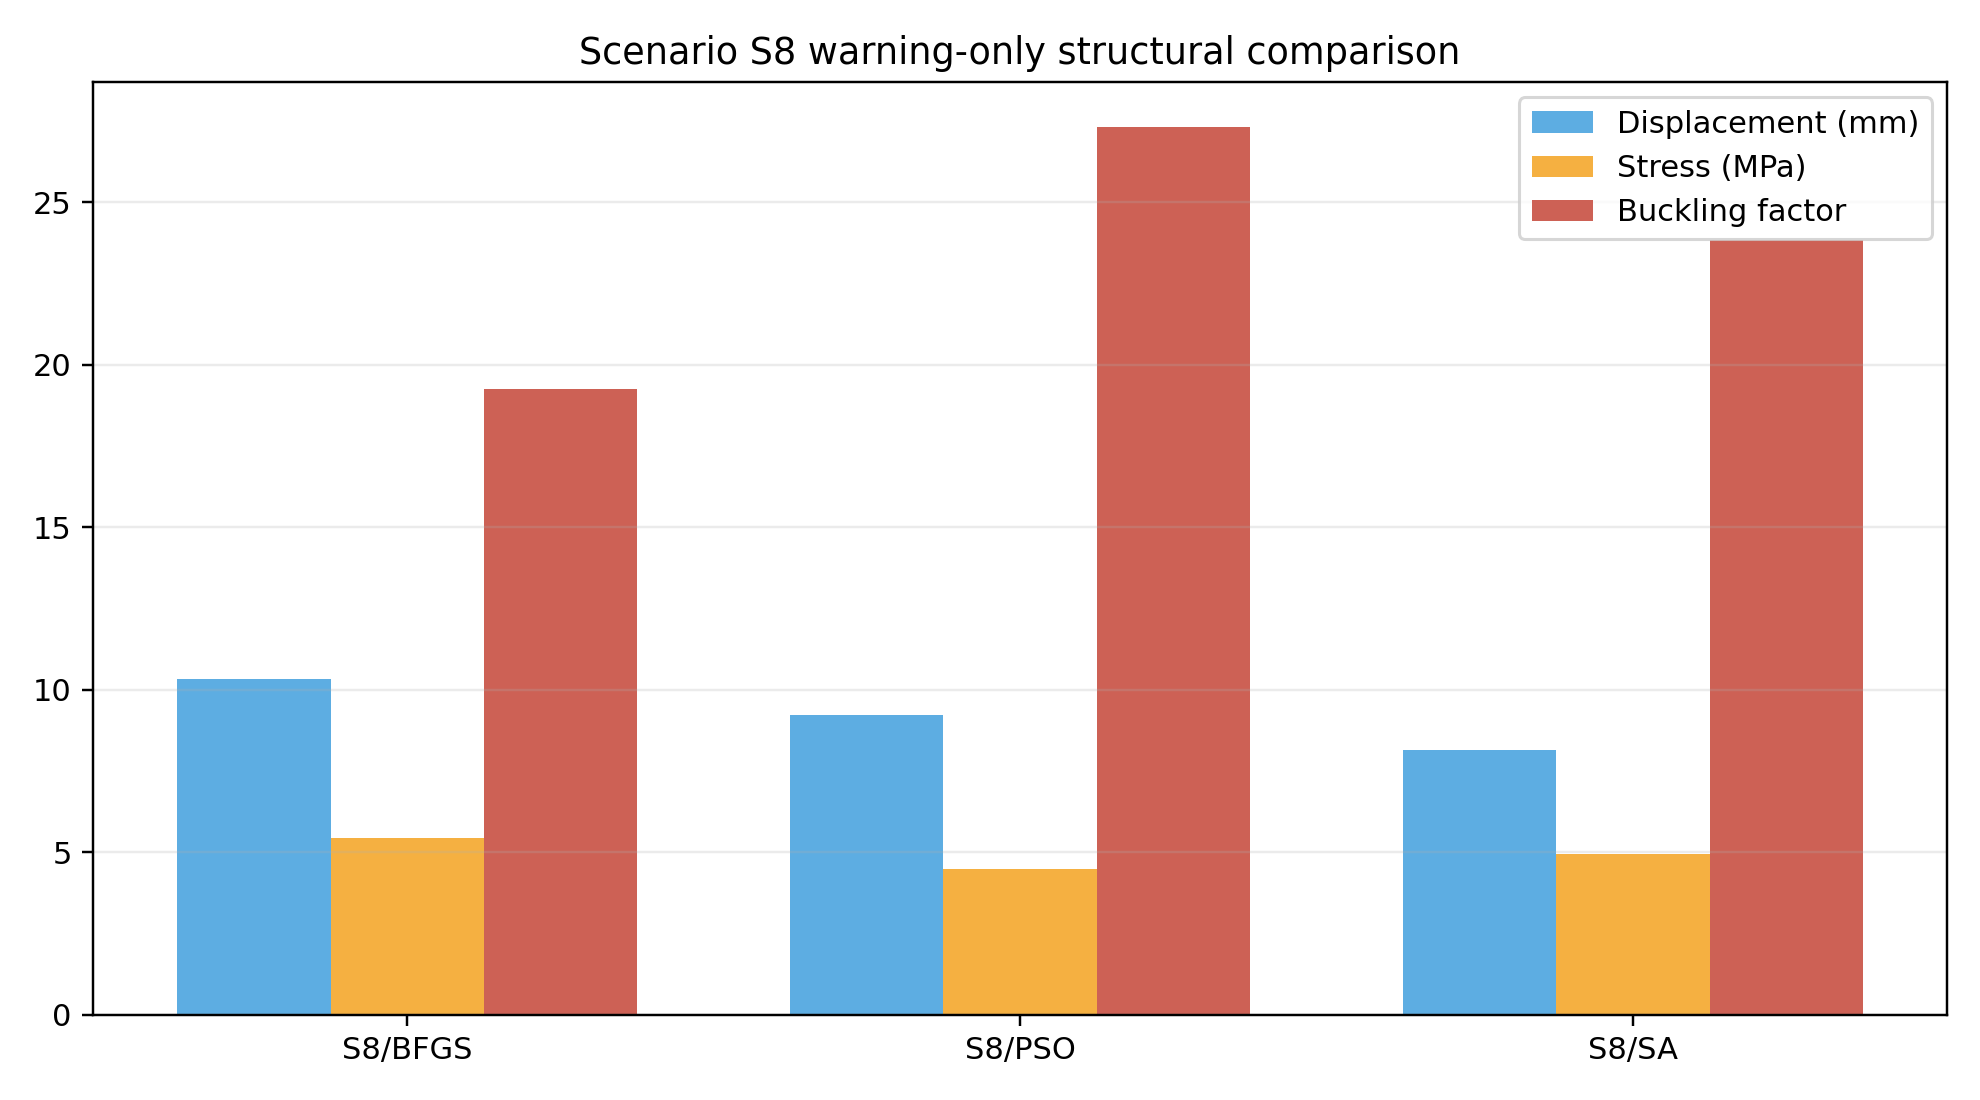
\includegraphics[width=0.95\textwidth]{../results/figures/s8_warning_metrics.png}
\caption{Scenario S8 warning metrics}
\end{figure}


\chapter{10. Field Visualizations of the Global Top-5}


\noindent All detailed field figures are rendered from actual Abaqus ODB data with Python, not from Abaqus screenshots.

\noindent Simulation geometry remains true-scale from Task 6. For readability, the rendered figures use a display-only vertical exaggeration of \texttt{1.35x} and a consistent left-to-right wind-view policy.

\noindent Wind arrows are bound to the configured physical wind axis (\texttt{+X}), so they indicate actual load direction rather than decorative annotation.

\noindent Per-case camera/arrow verification is enforced numerically through \texttt{plot\_view\_audit.csv}: the camera is perpendicular to wind direction, wind projects left-to-right on screen, and arrows stay outside the tower silhouette.


\section{S7 / BFGS}


\begin{figure}[H]
\centering
\begin{subfigure}{0.32\textwidth}
\centering
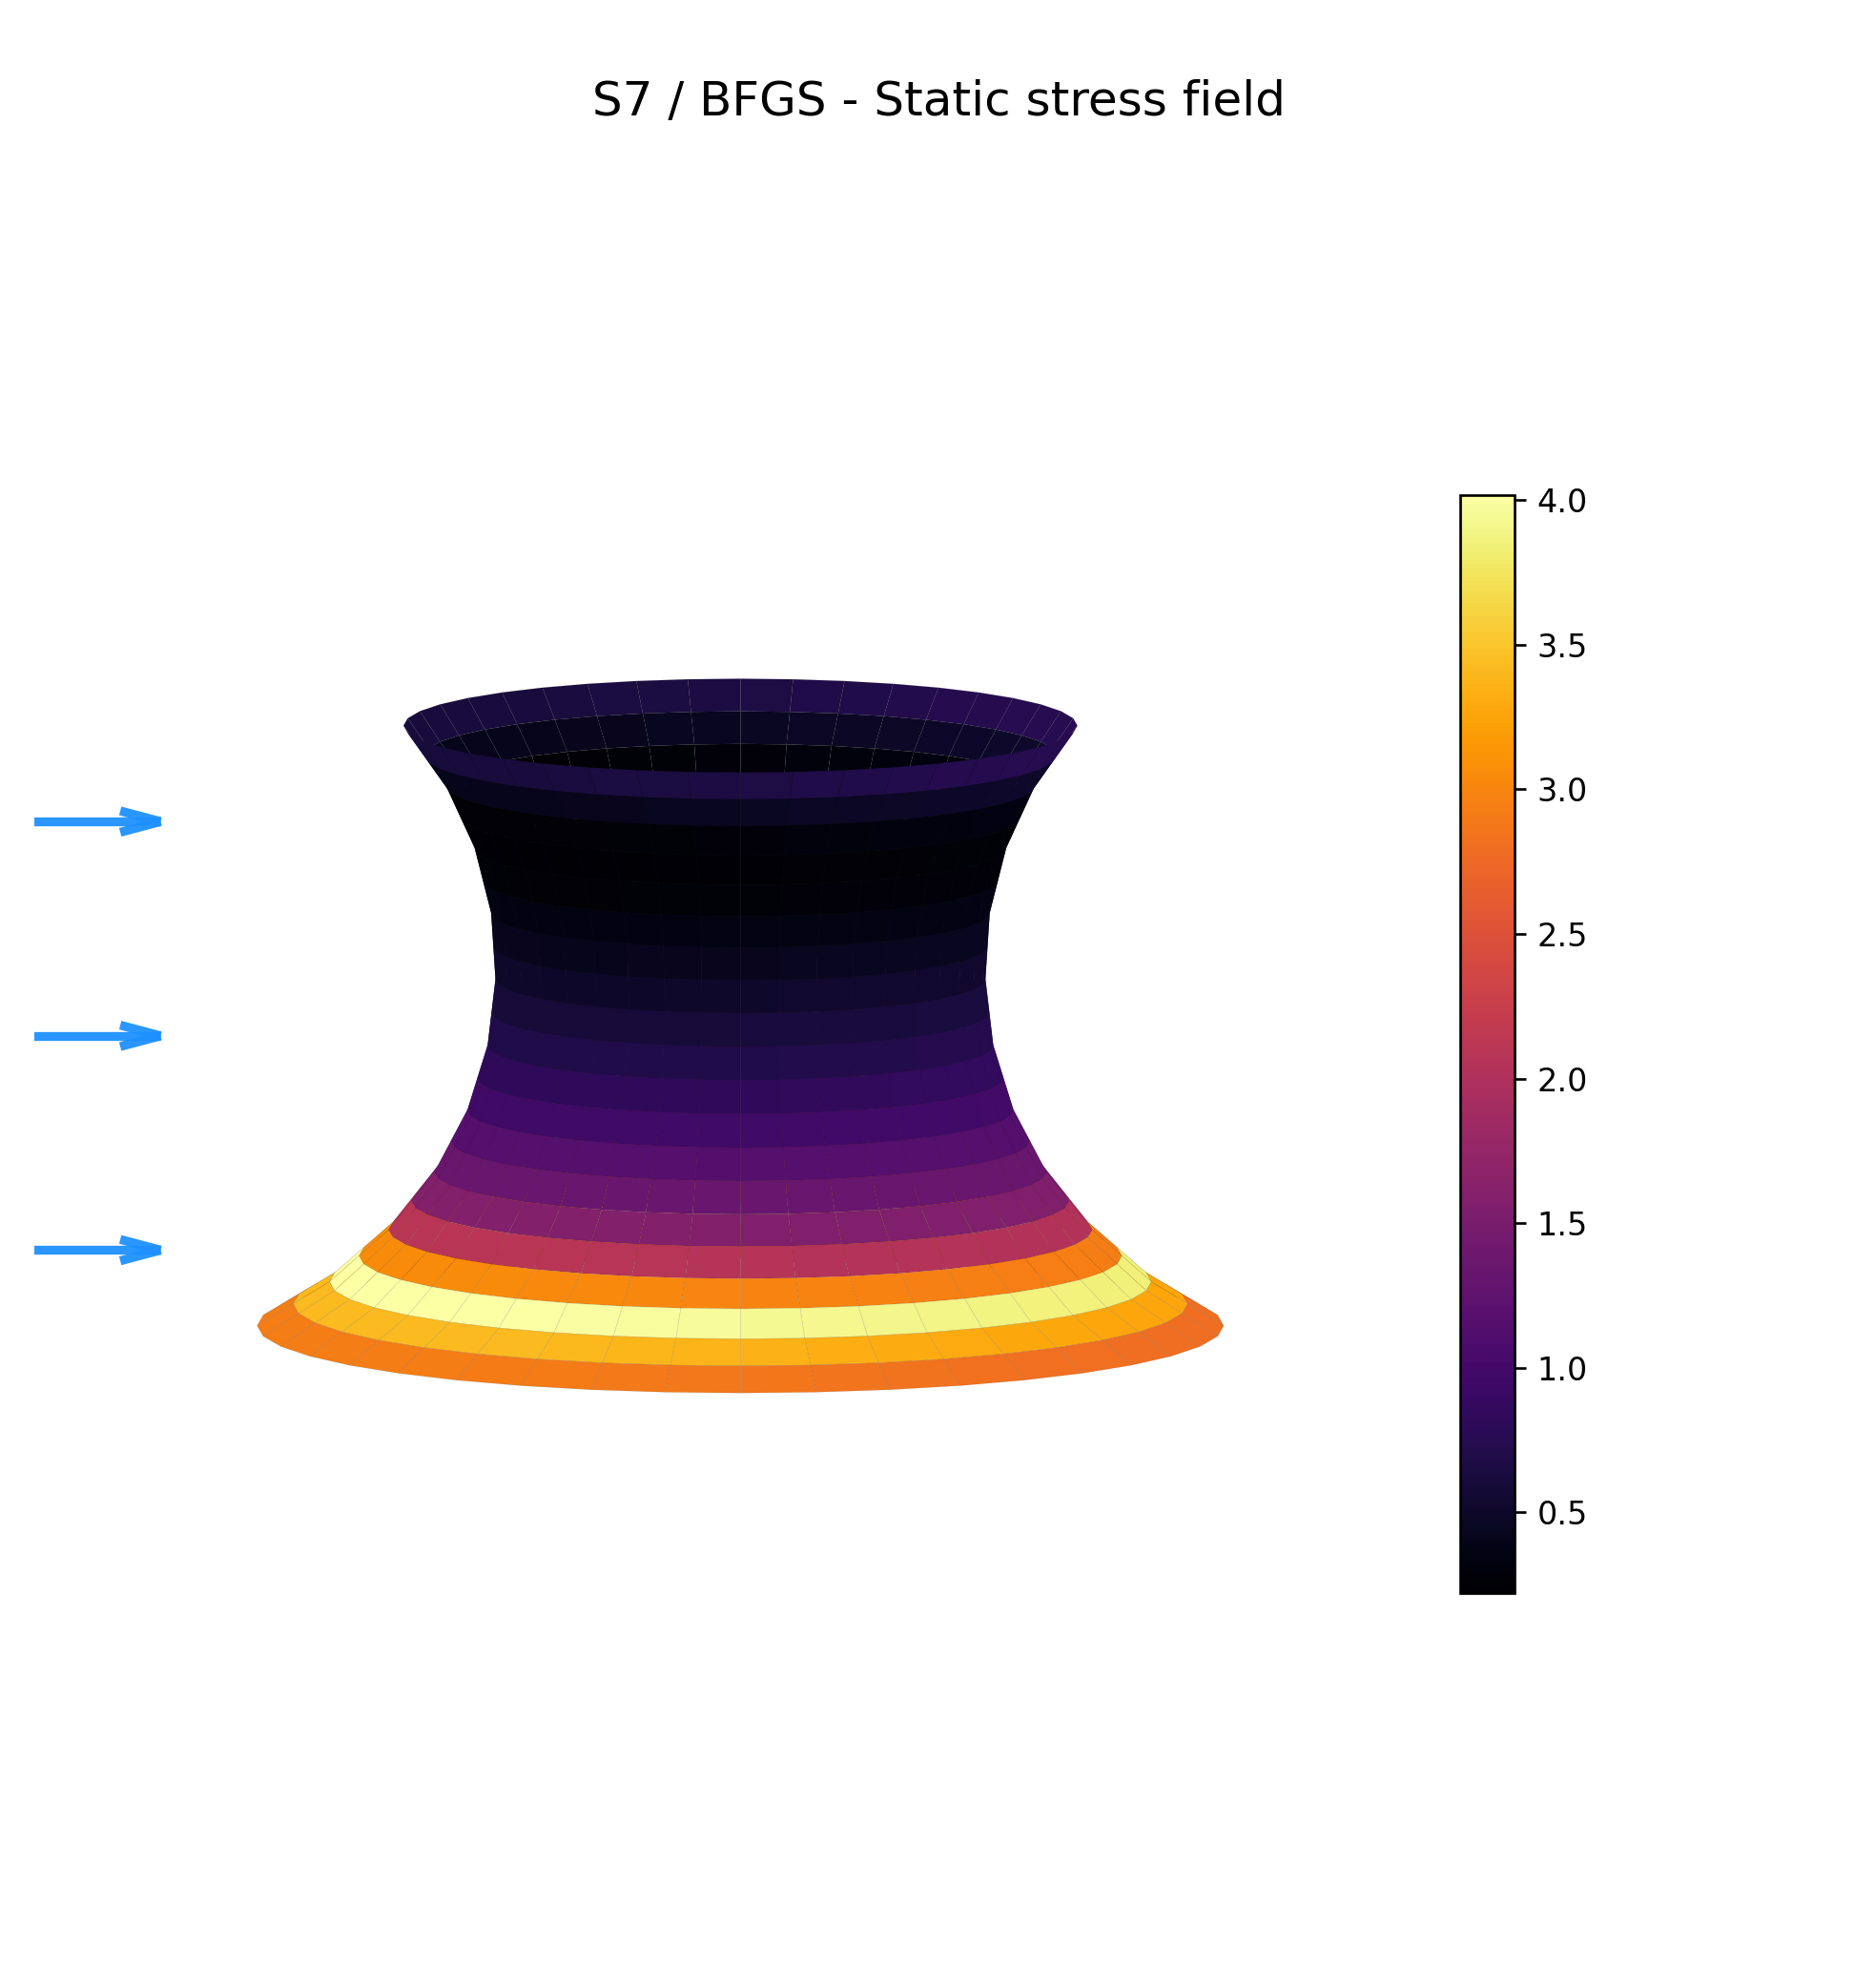
\includegraphics[width=\textwidth]{../results/figures/task7_s7_bfgs_stress.png}
\caption{S7 / BFGS stress}
\end{subfigure}\hfill
\begin{subfigure}{0.32\textwidth}
\centering
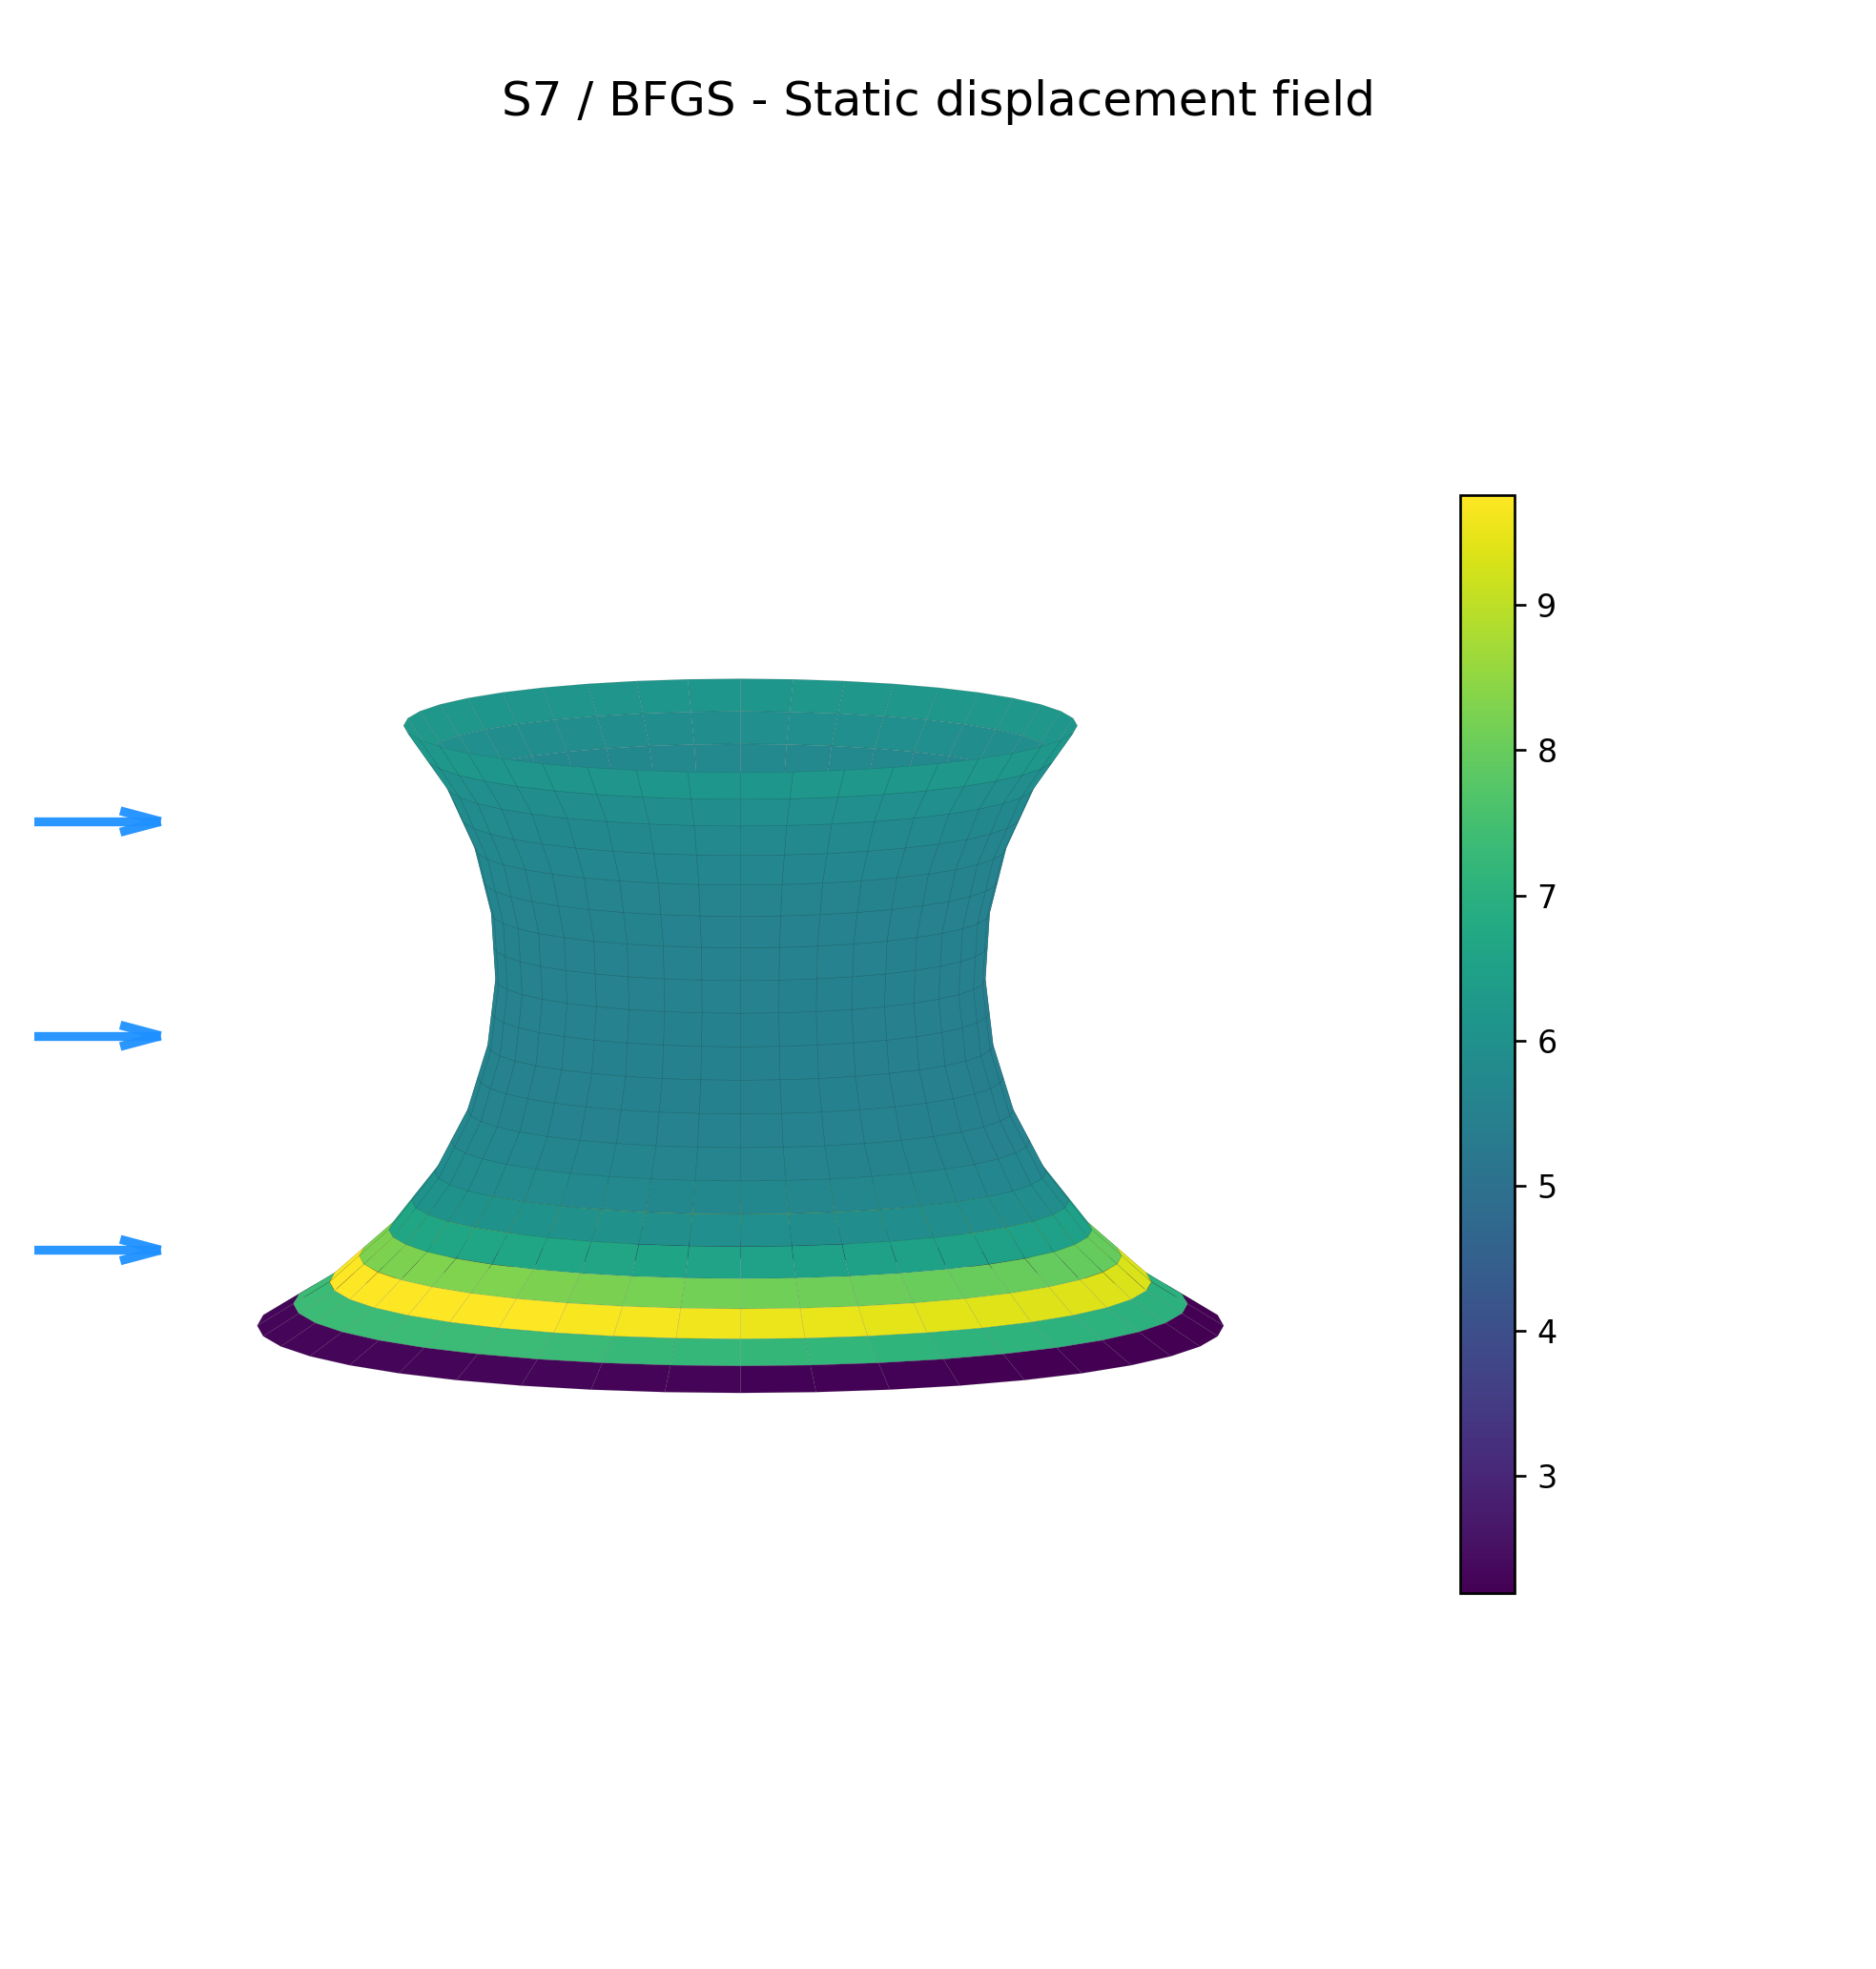
\includegraphics[width=\textwidth]{../results/figures/task7_s7_bfgs_displacement.png}
\caption{S7 / BFGS displacement}
\end{subfigure}\hfill
\begin{subfigure}{0.32\textwidth}
\centering
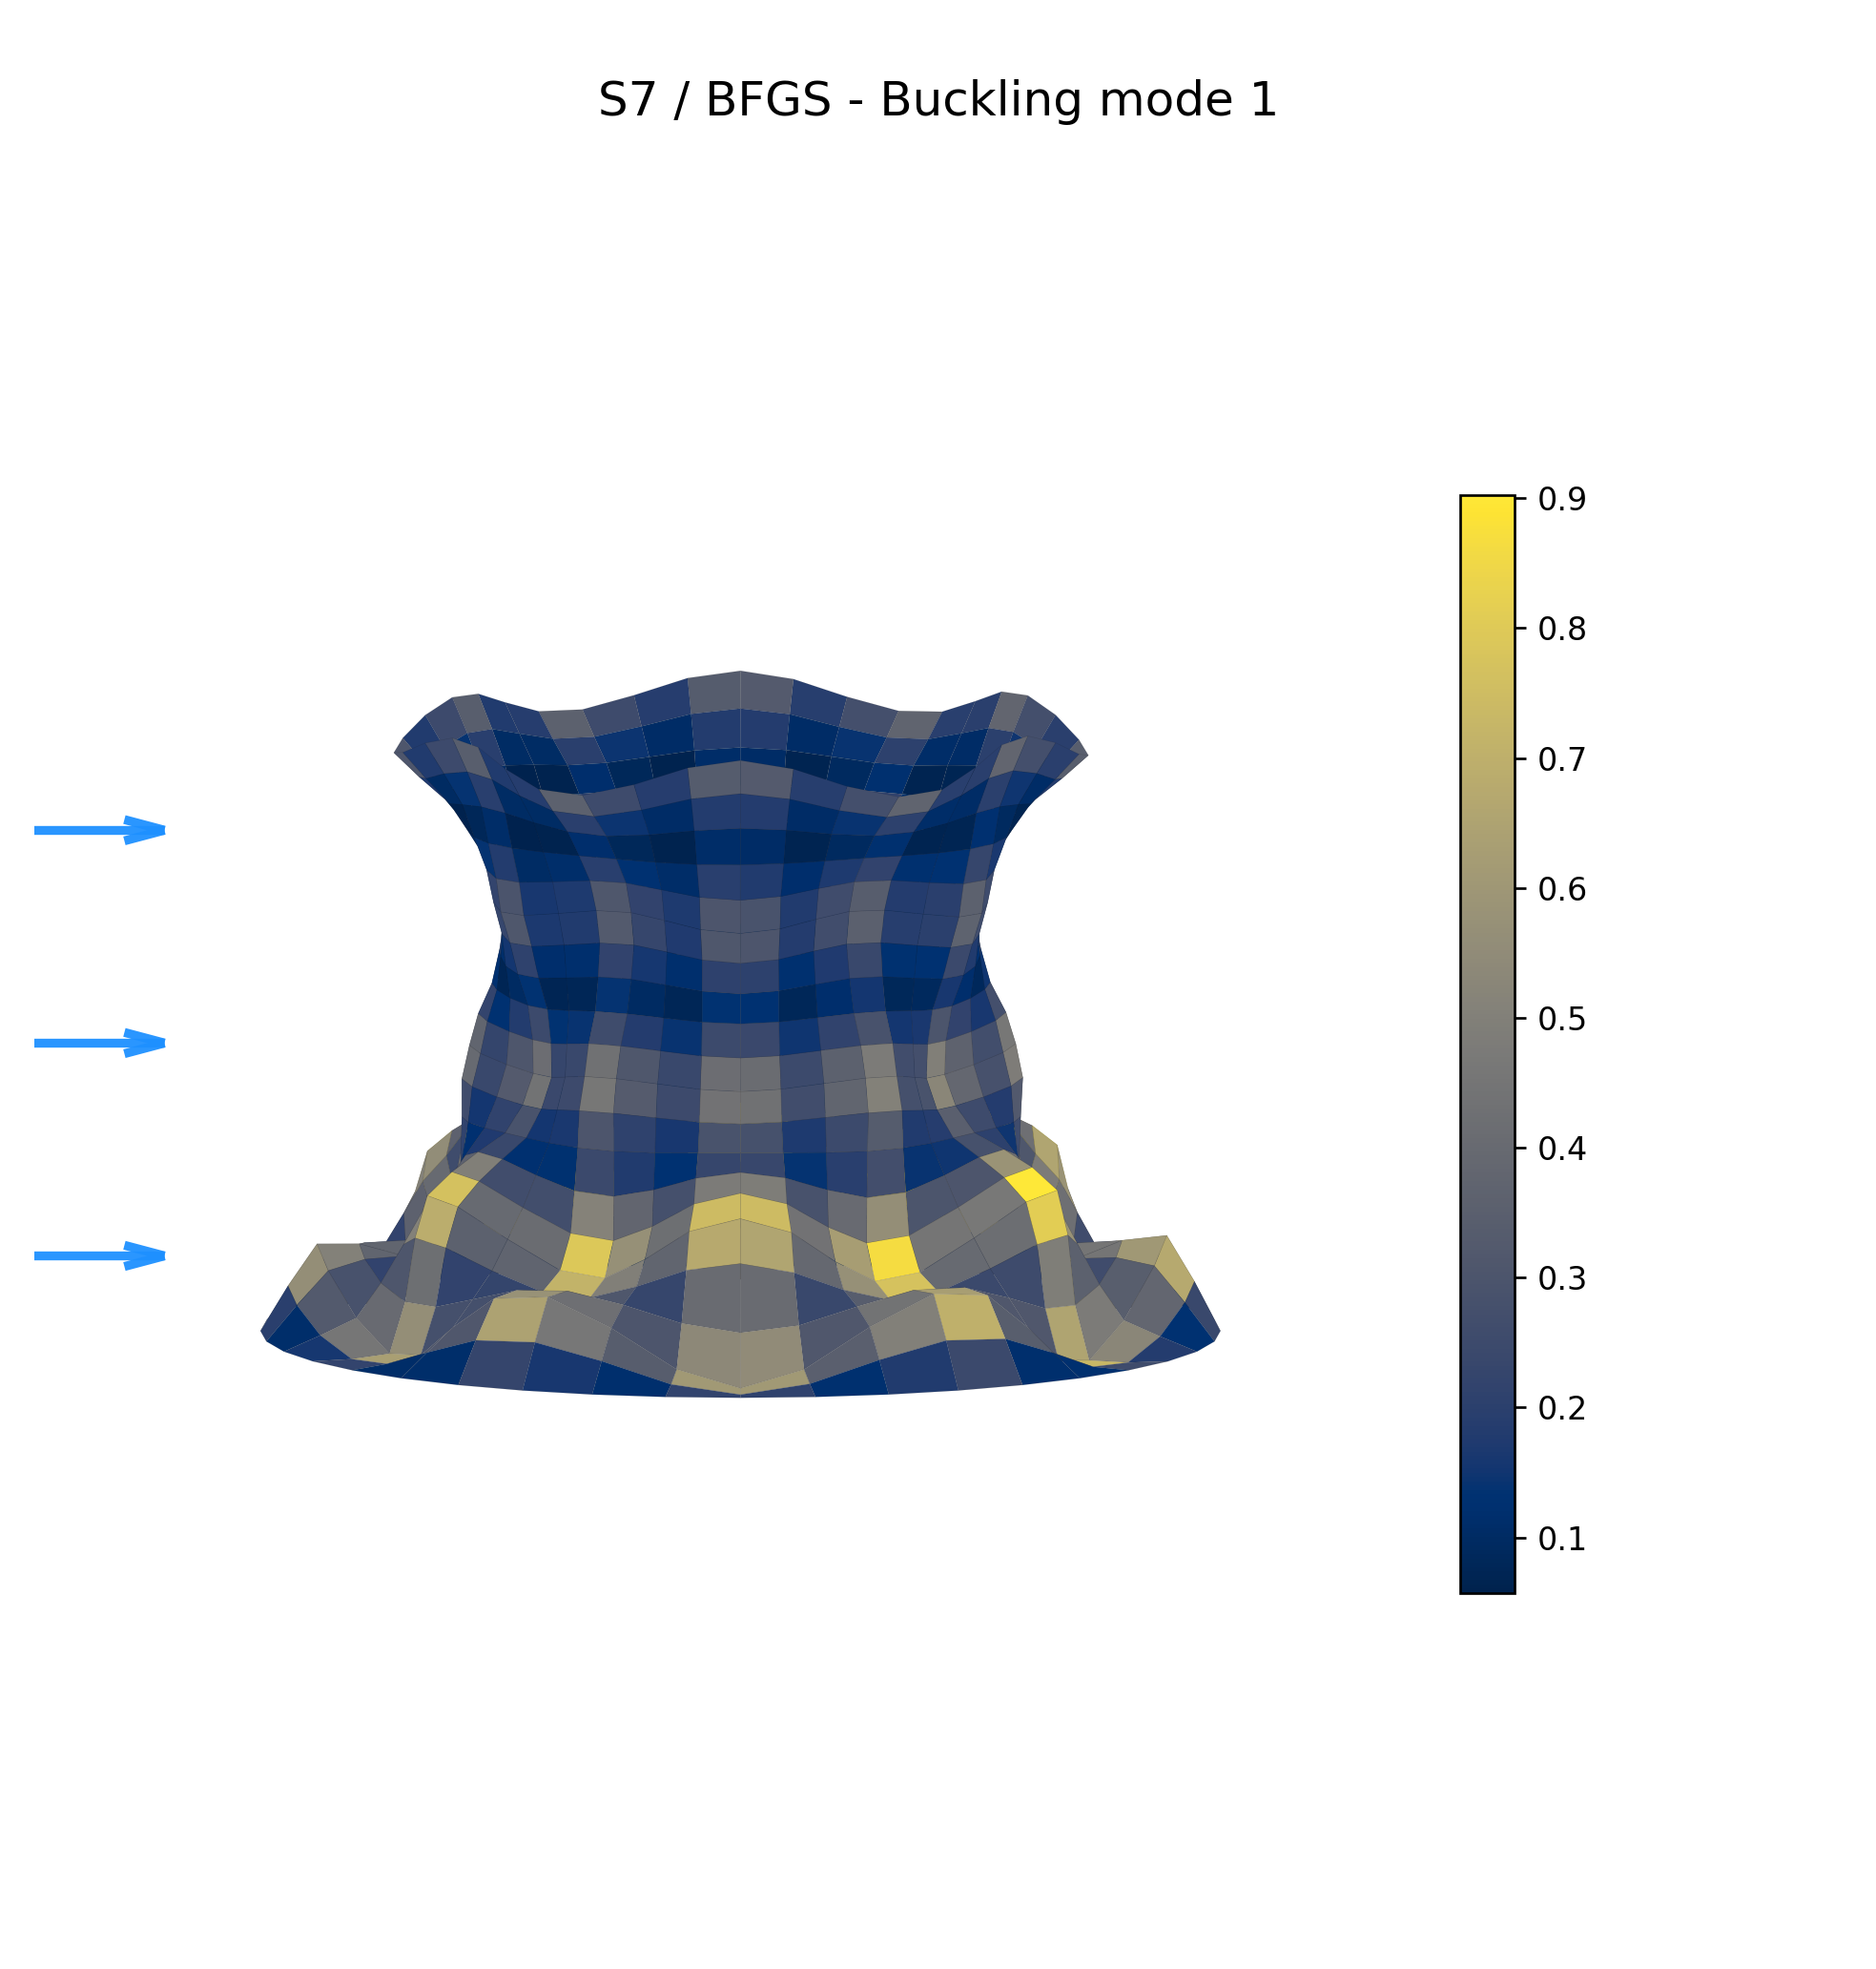
\includegraphics[width=\textwidth]{../results/figures/task7_s7_bfgs_buckling_mode1.png}
\caption{S7 / BFGS buckling}
\end{subfigure}
\caption{Combined visual fields}
\end{figure}


\noindent \textbf{Performance Discussion (Rank 1):} The \texttt{S7 / BFGS} model (Engineering-feasible) achieved an overall weighted score of \texttt{6.750}. It demonstrates strong structural integrity with a first buckling factor of \texttt{24.948}. Under the applied wind load, the maximum observed displacement is bounded at \texttt{10.105 mm}, and peak von Mises stresses reach \texttt{4.134 MPa}. As the top-ranked candidate, this geometry offers the most convincing balance of minimal material footprint, acceptable deflection, and a high margin against linear buckling.


\section{S3 / SA}


\begin{figure}[H]
\centering
\begin{subfigure}{0.32\textwidth}
\centering
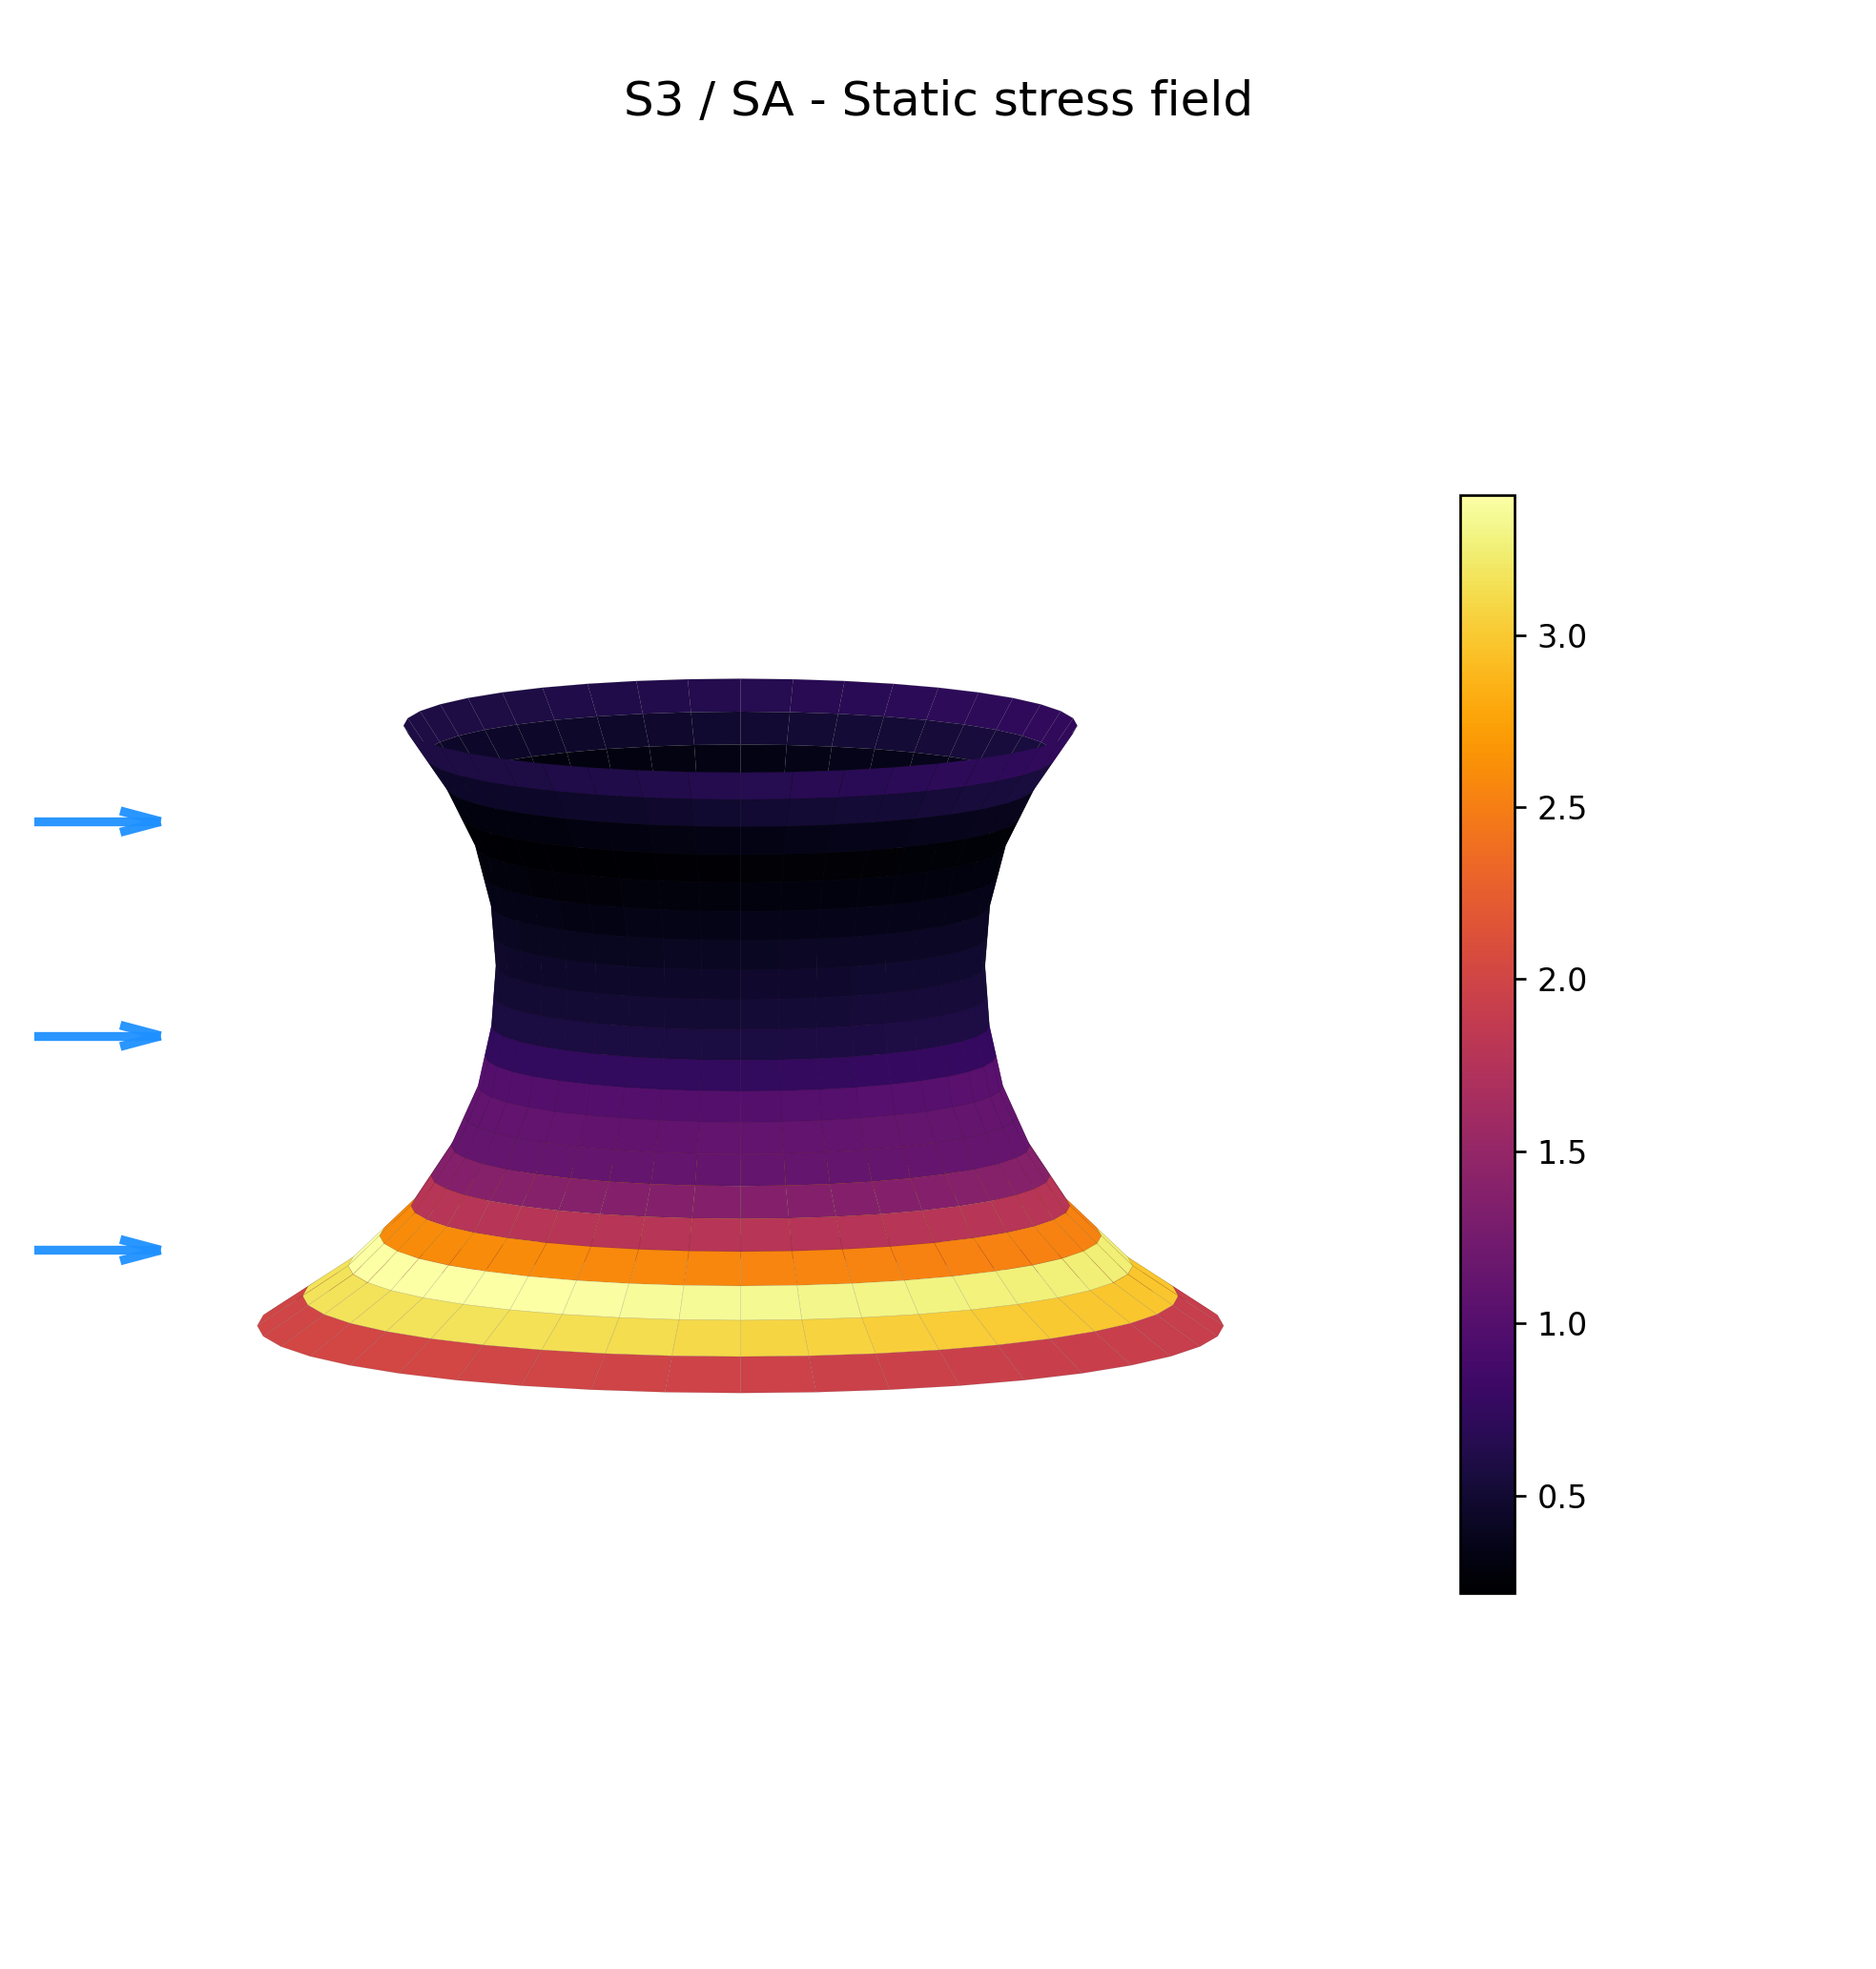
\includegraphics[width=\textwidth]{../results/figures/task7_s3_sa_stress.png}
\caption{S3 / SA stress}
\end{subfigure}\hfill
\begin{subfigure}{0.32\textwidth}
\centering
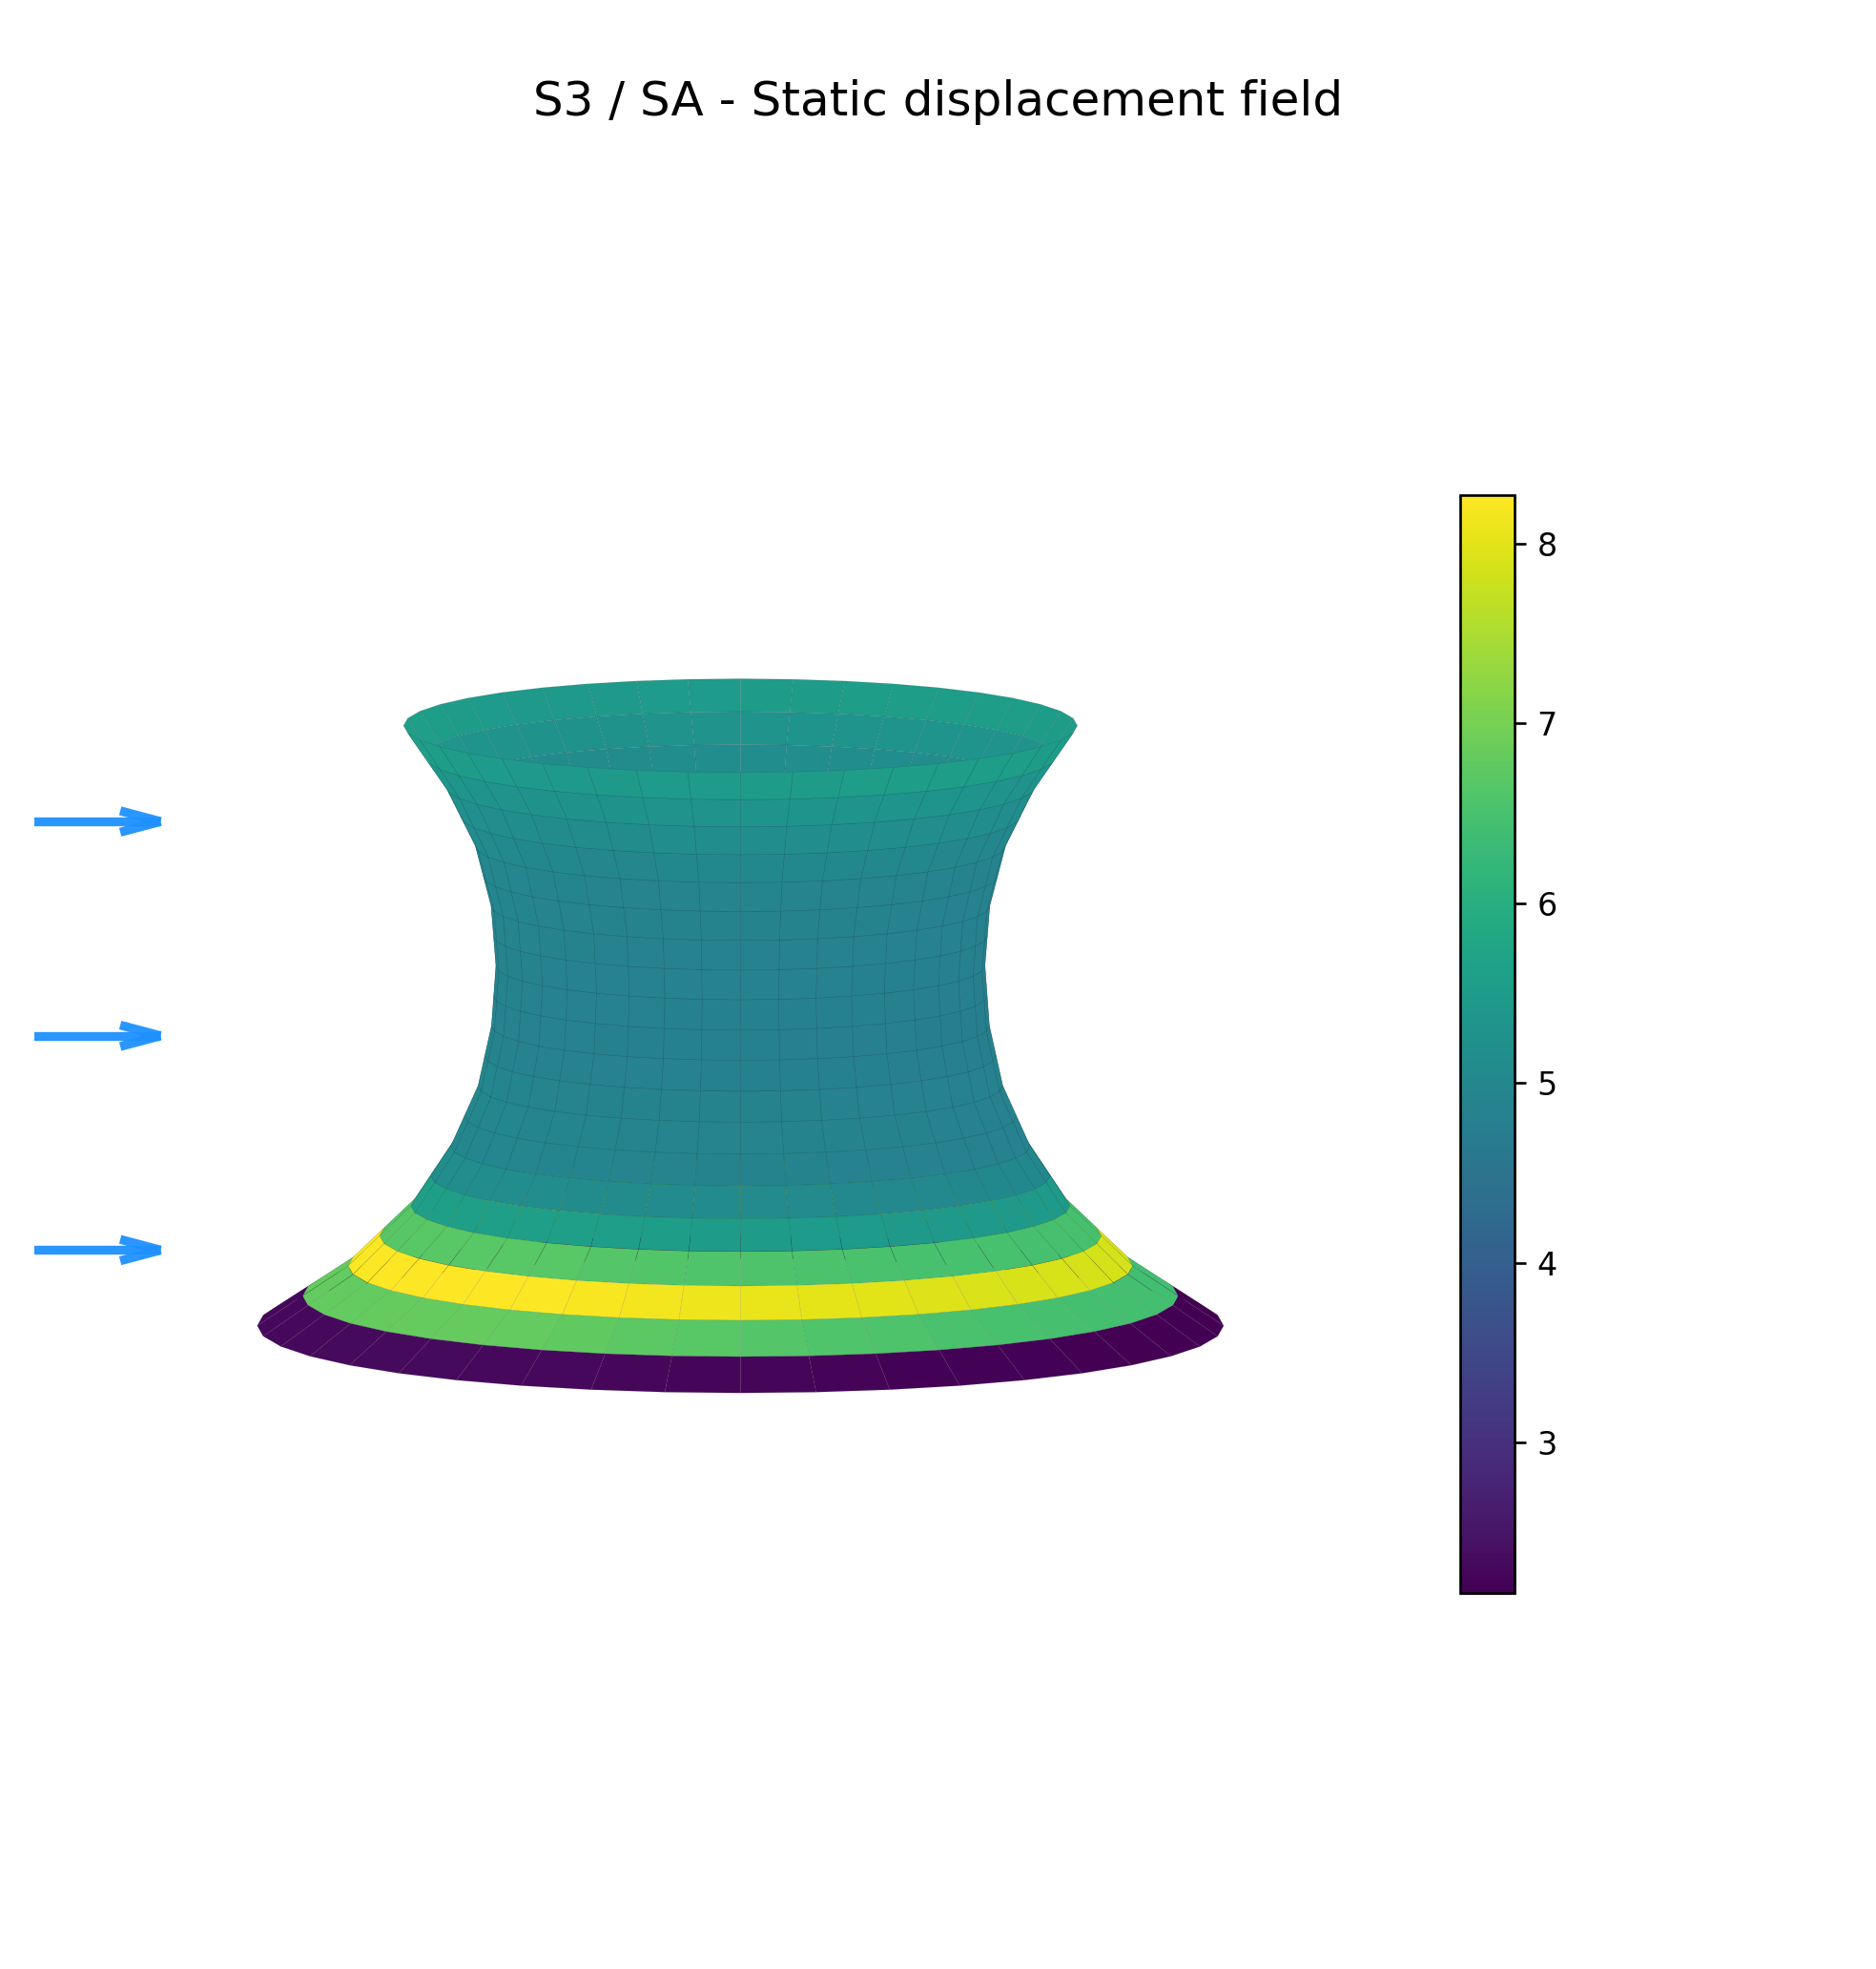
\includegraphics[width=\textwidth]{../results/figures/task7_s3_sa_displacement.png}
\caption{S3 / SA displacement}
\end{subfigure}\hfill
\begin{subfigure}{0.32\textwidth}
\centering
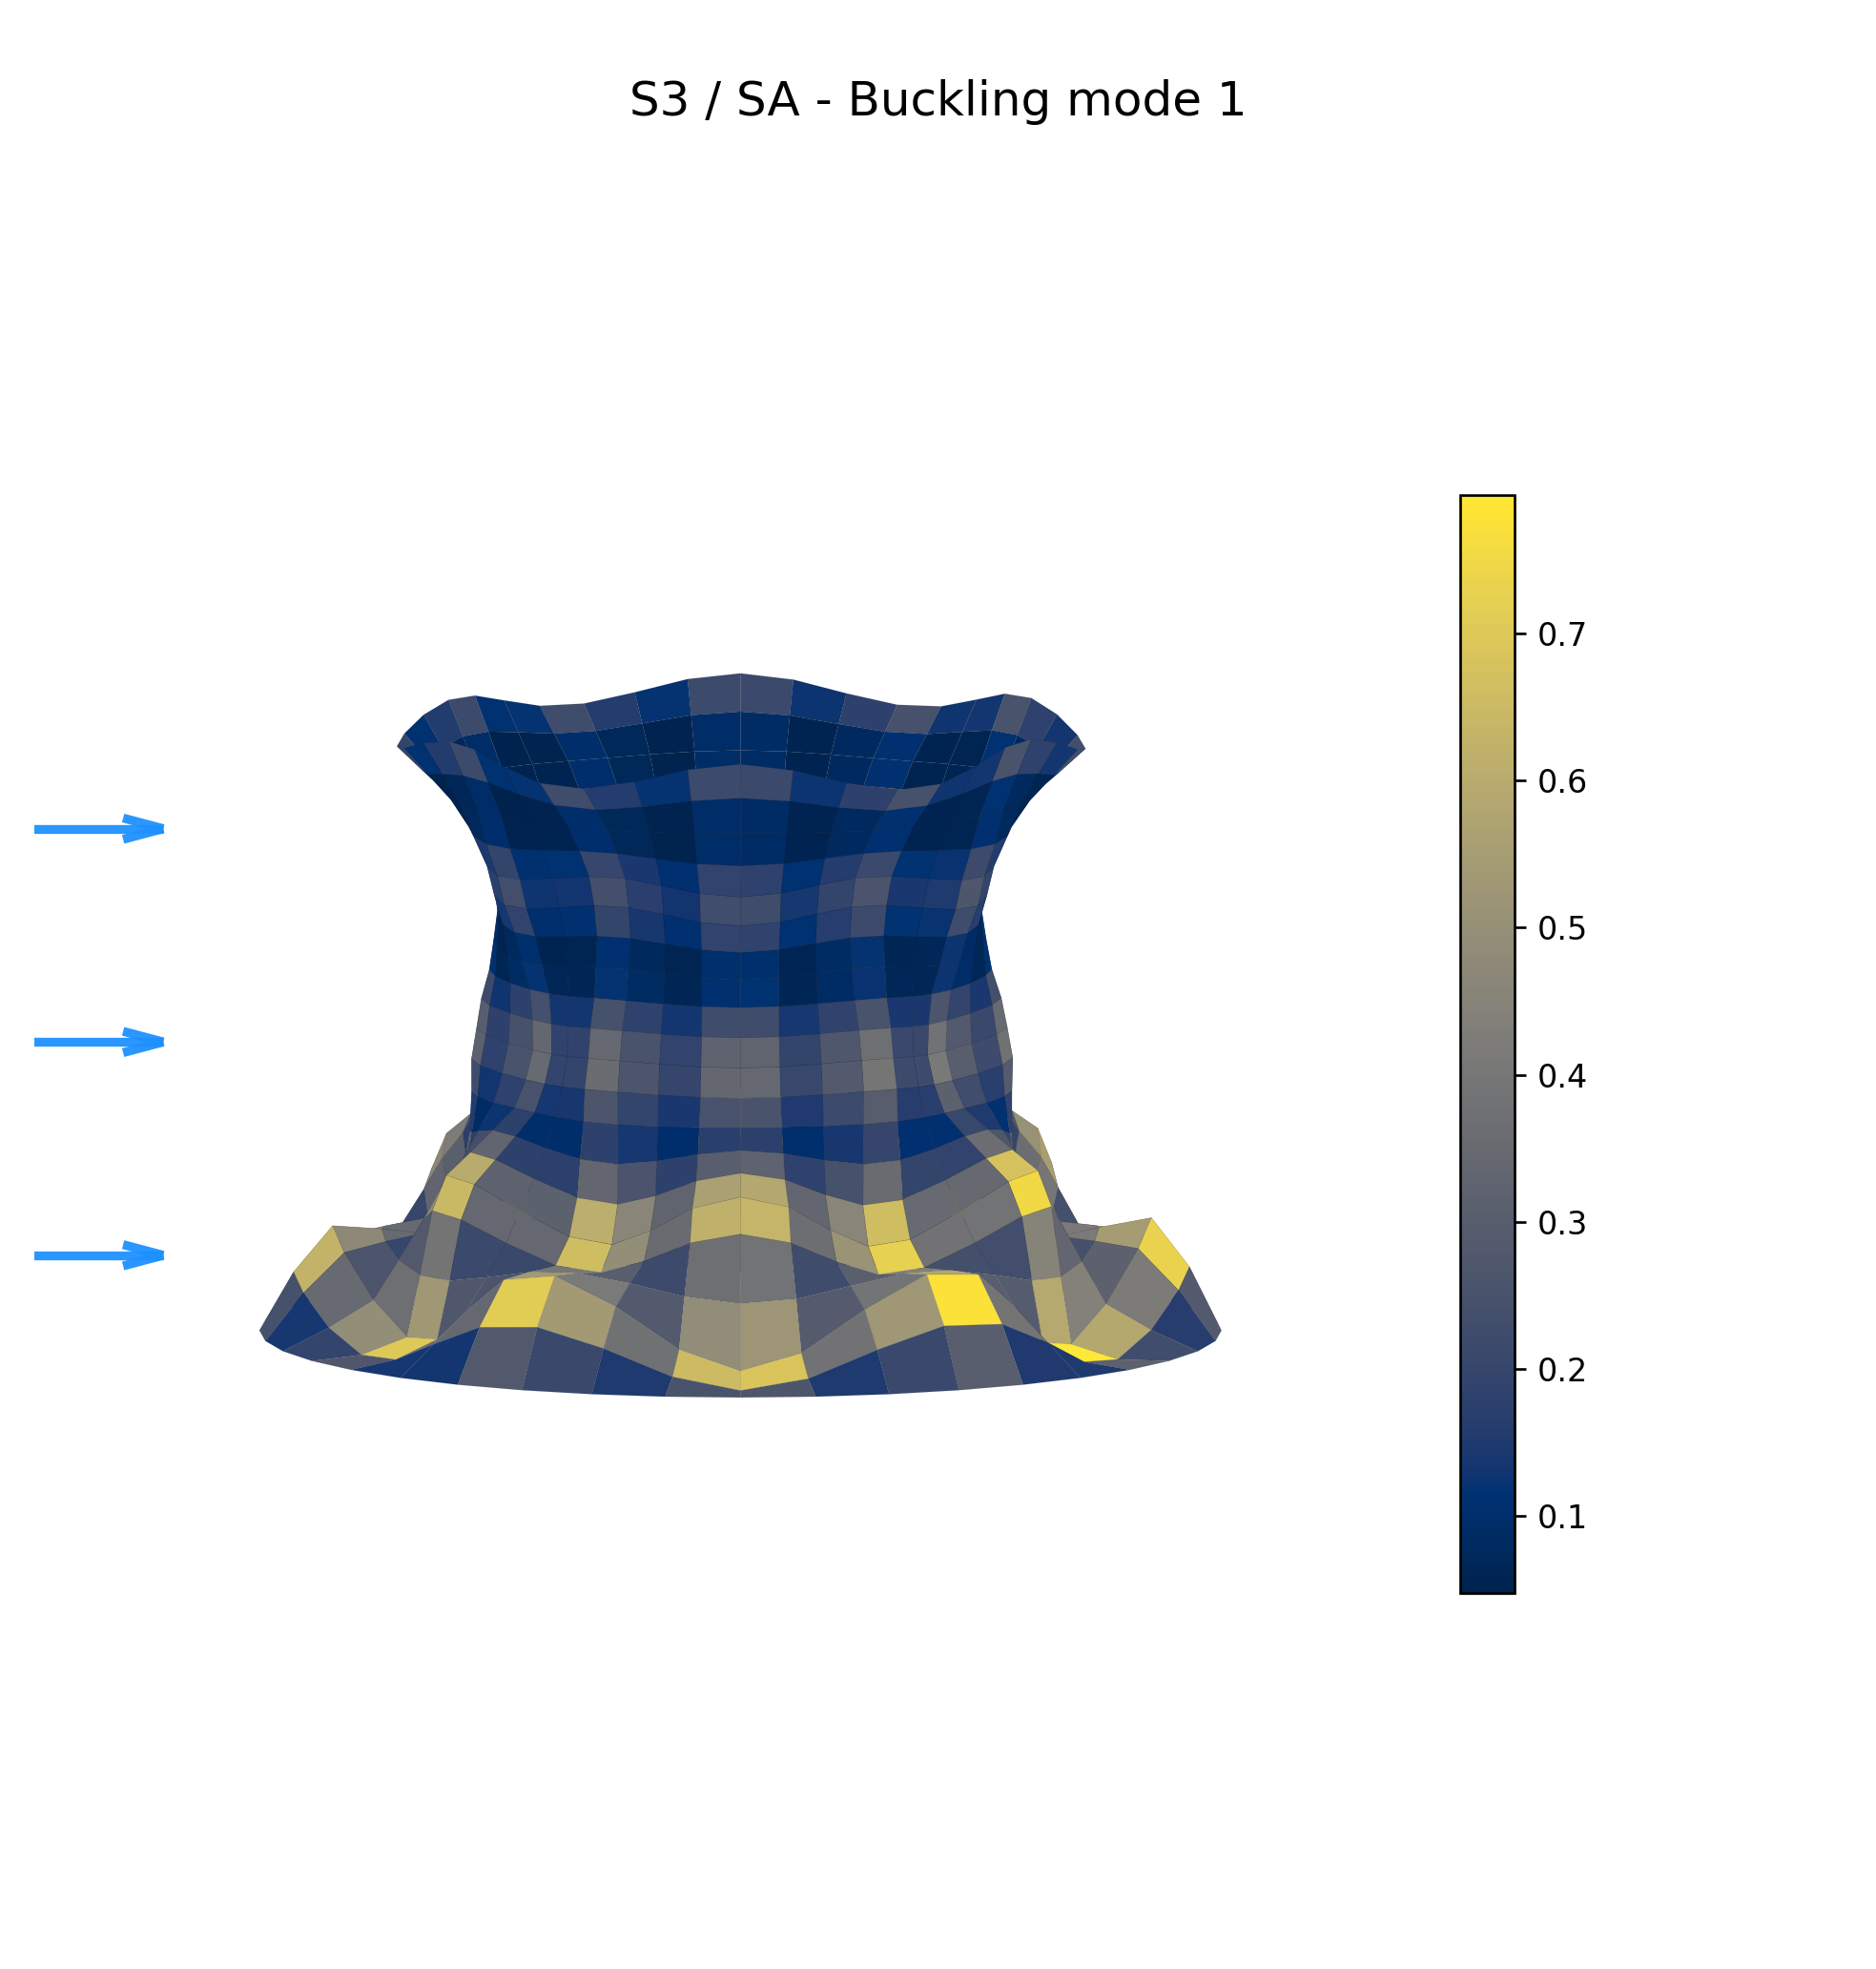
\includegraphics[width=\textwidth]{../results/figures/task7_s3_sa_buckling_mode1.png}
\caption{S3 / SA buckling}
\end{subfigure}
\caption{Combined visual fields}
\end{figure}


\noindent \textbf{Performance Discussion (Rank 2):} The \texttt{S3 / SA} model (Engineering-feasible) achieved an overall weighted score of \texttt{7.050}. It demonstrates strong structural integrity with a first buckling factor of \texttt{23.834}. Under the applied wind load, the maximum observed displacement is bounded at \texttt{9.036 mm}, and peak von Mises stresses reach \texttt{3.526 MPa}. As a high-ranking runner-up, it presents an extremely competitive alternative, trading minimal surface area differences for robust stress and displacement behavior.


\section{S2 / SA}


\begin{figure}[H]
\centering
\begin{subfigure}{0.32\textwidth}
\centering
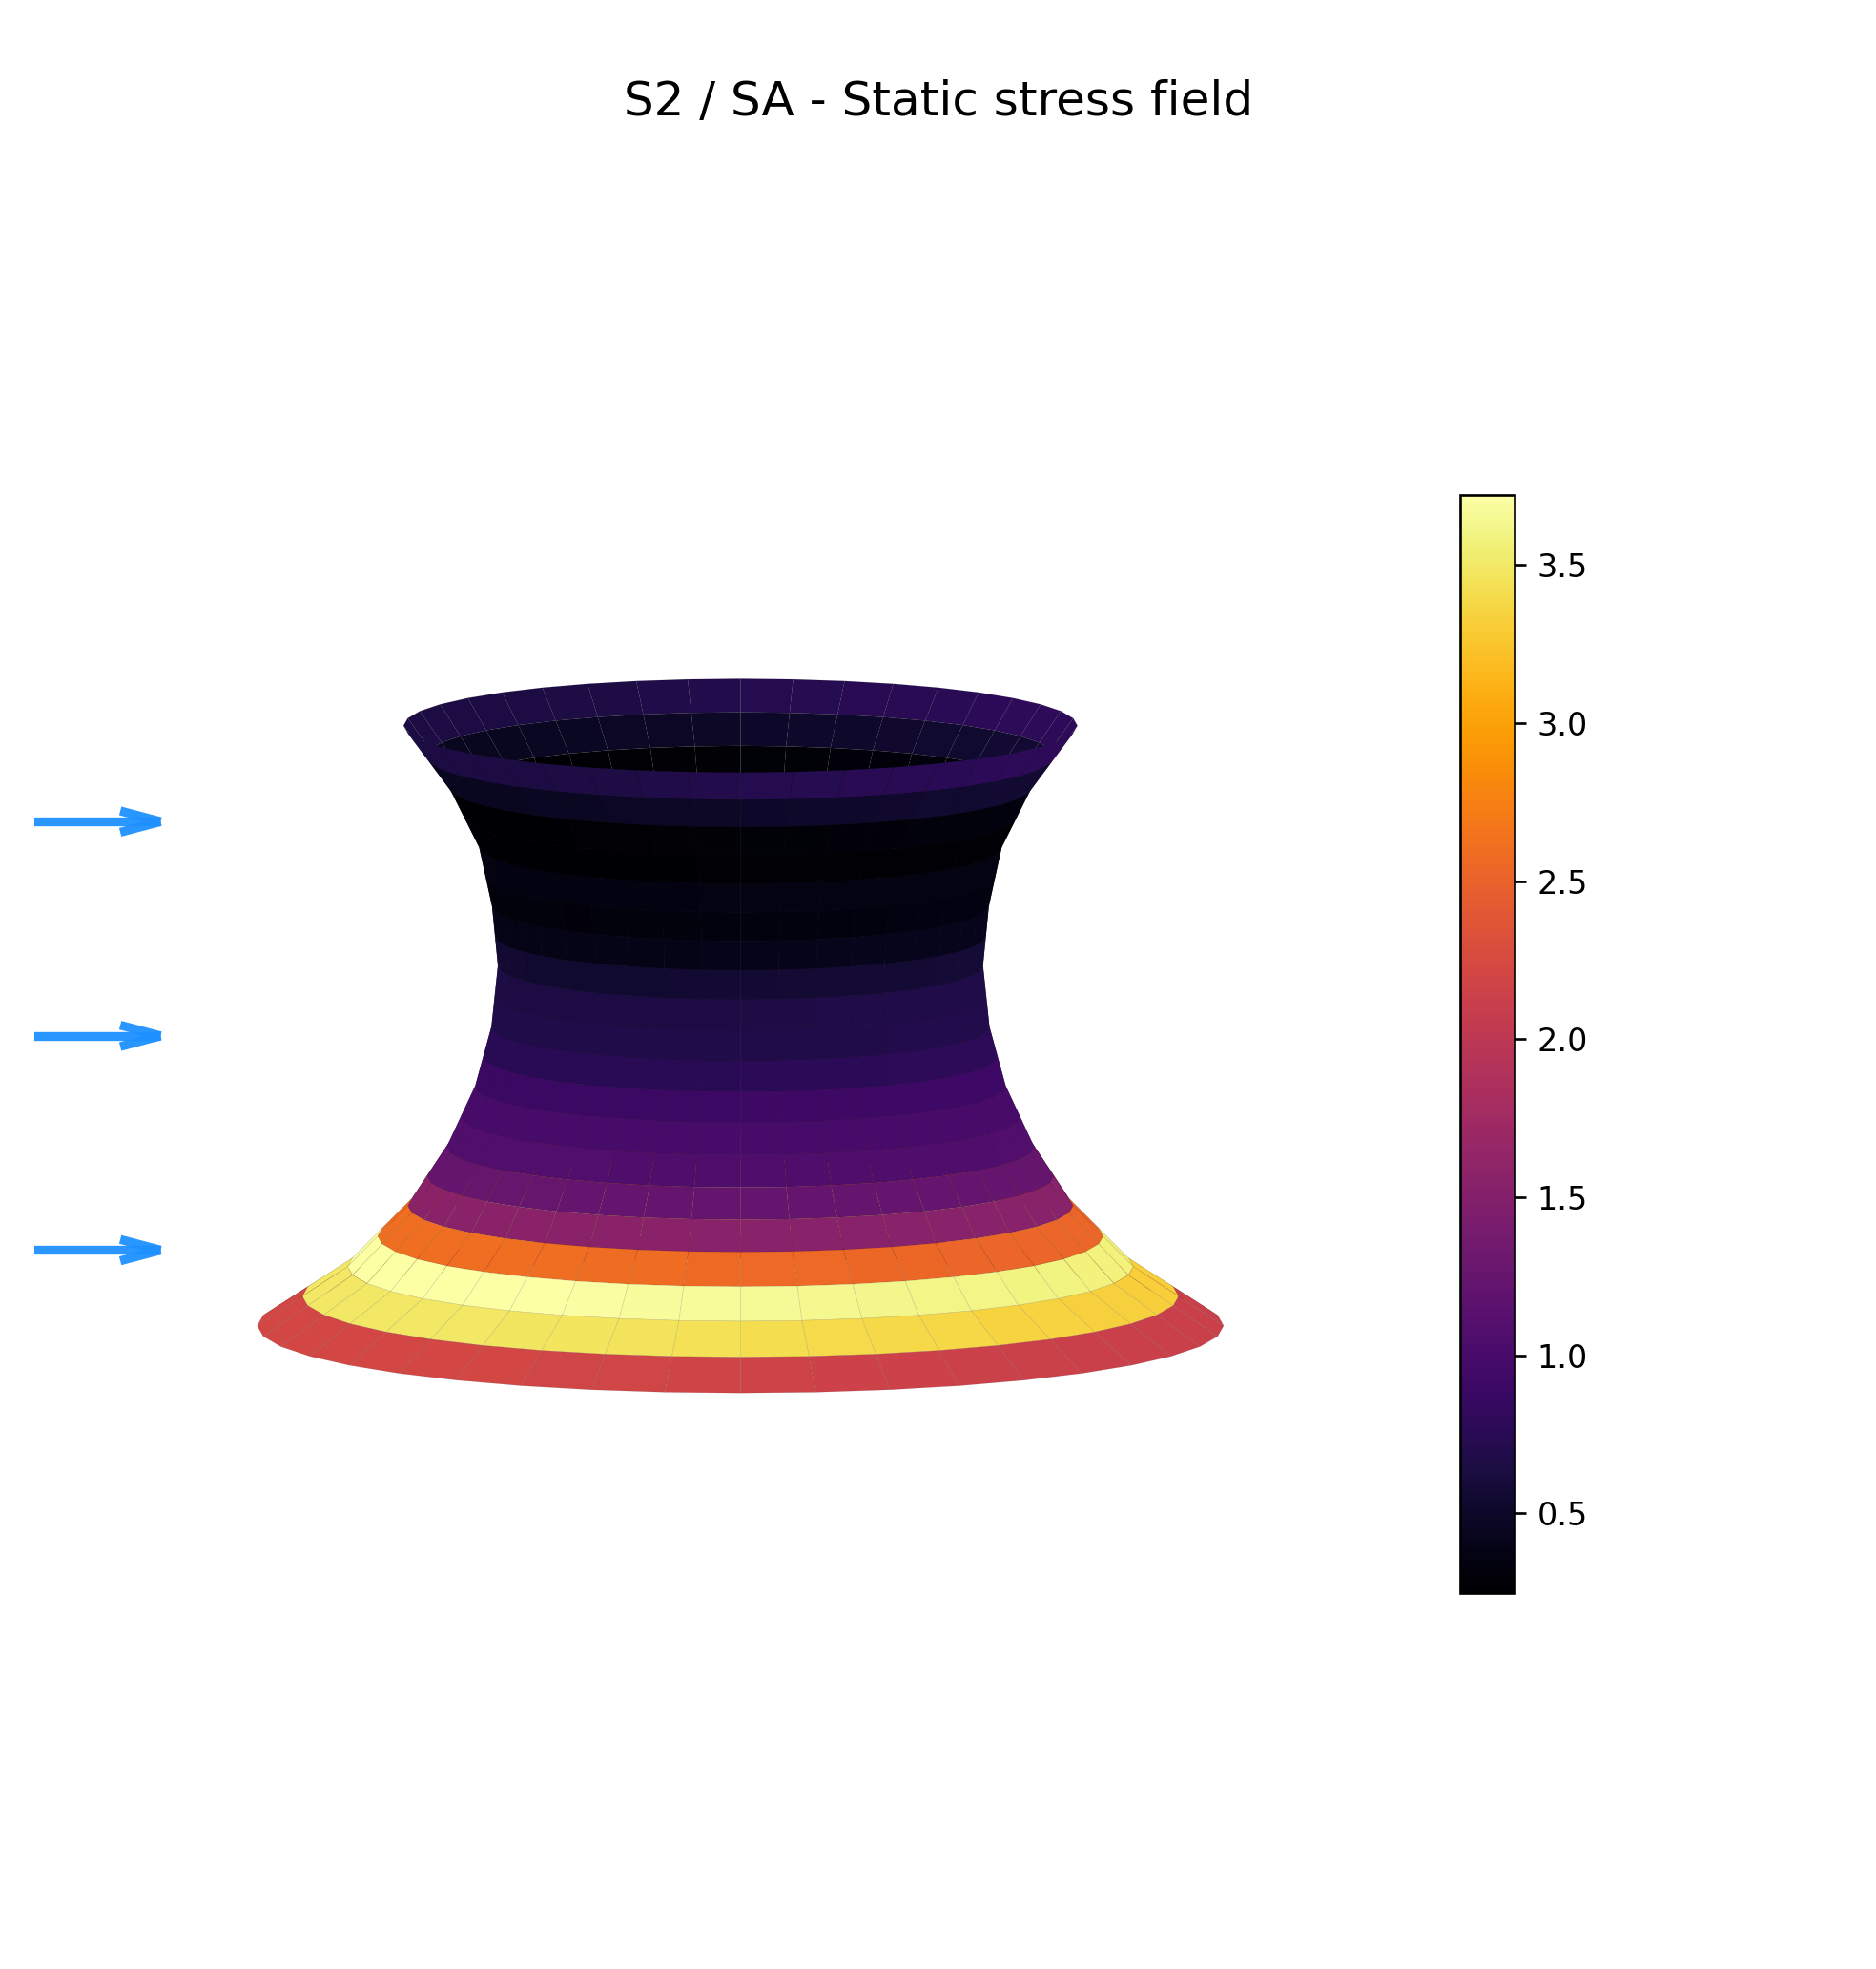
\includegraphics[width=\textwidth]{../results/figures/task7_s2_sa_stress.png}
\caption{S2 / SA stress}
\end{subfigure}\hfill
\begin{subfigure}{0.32\textwidth}
\centering
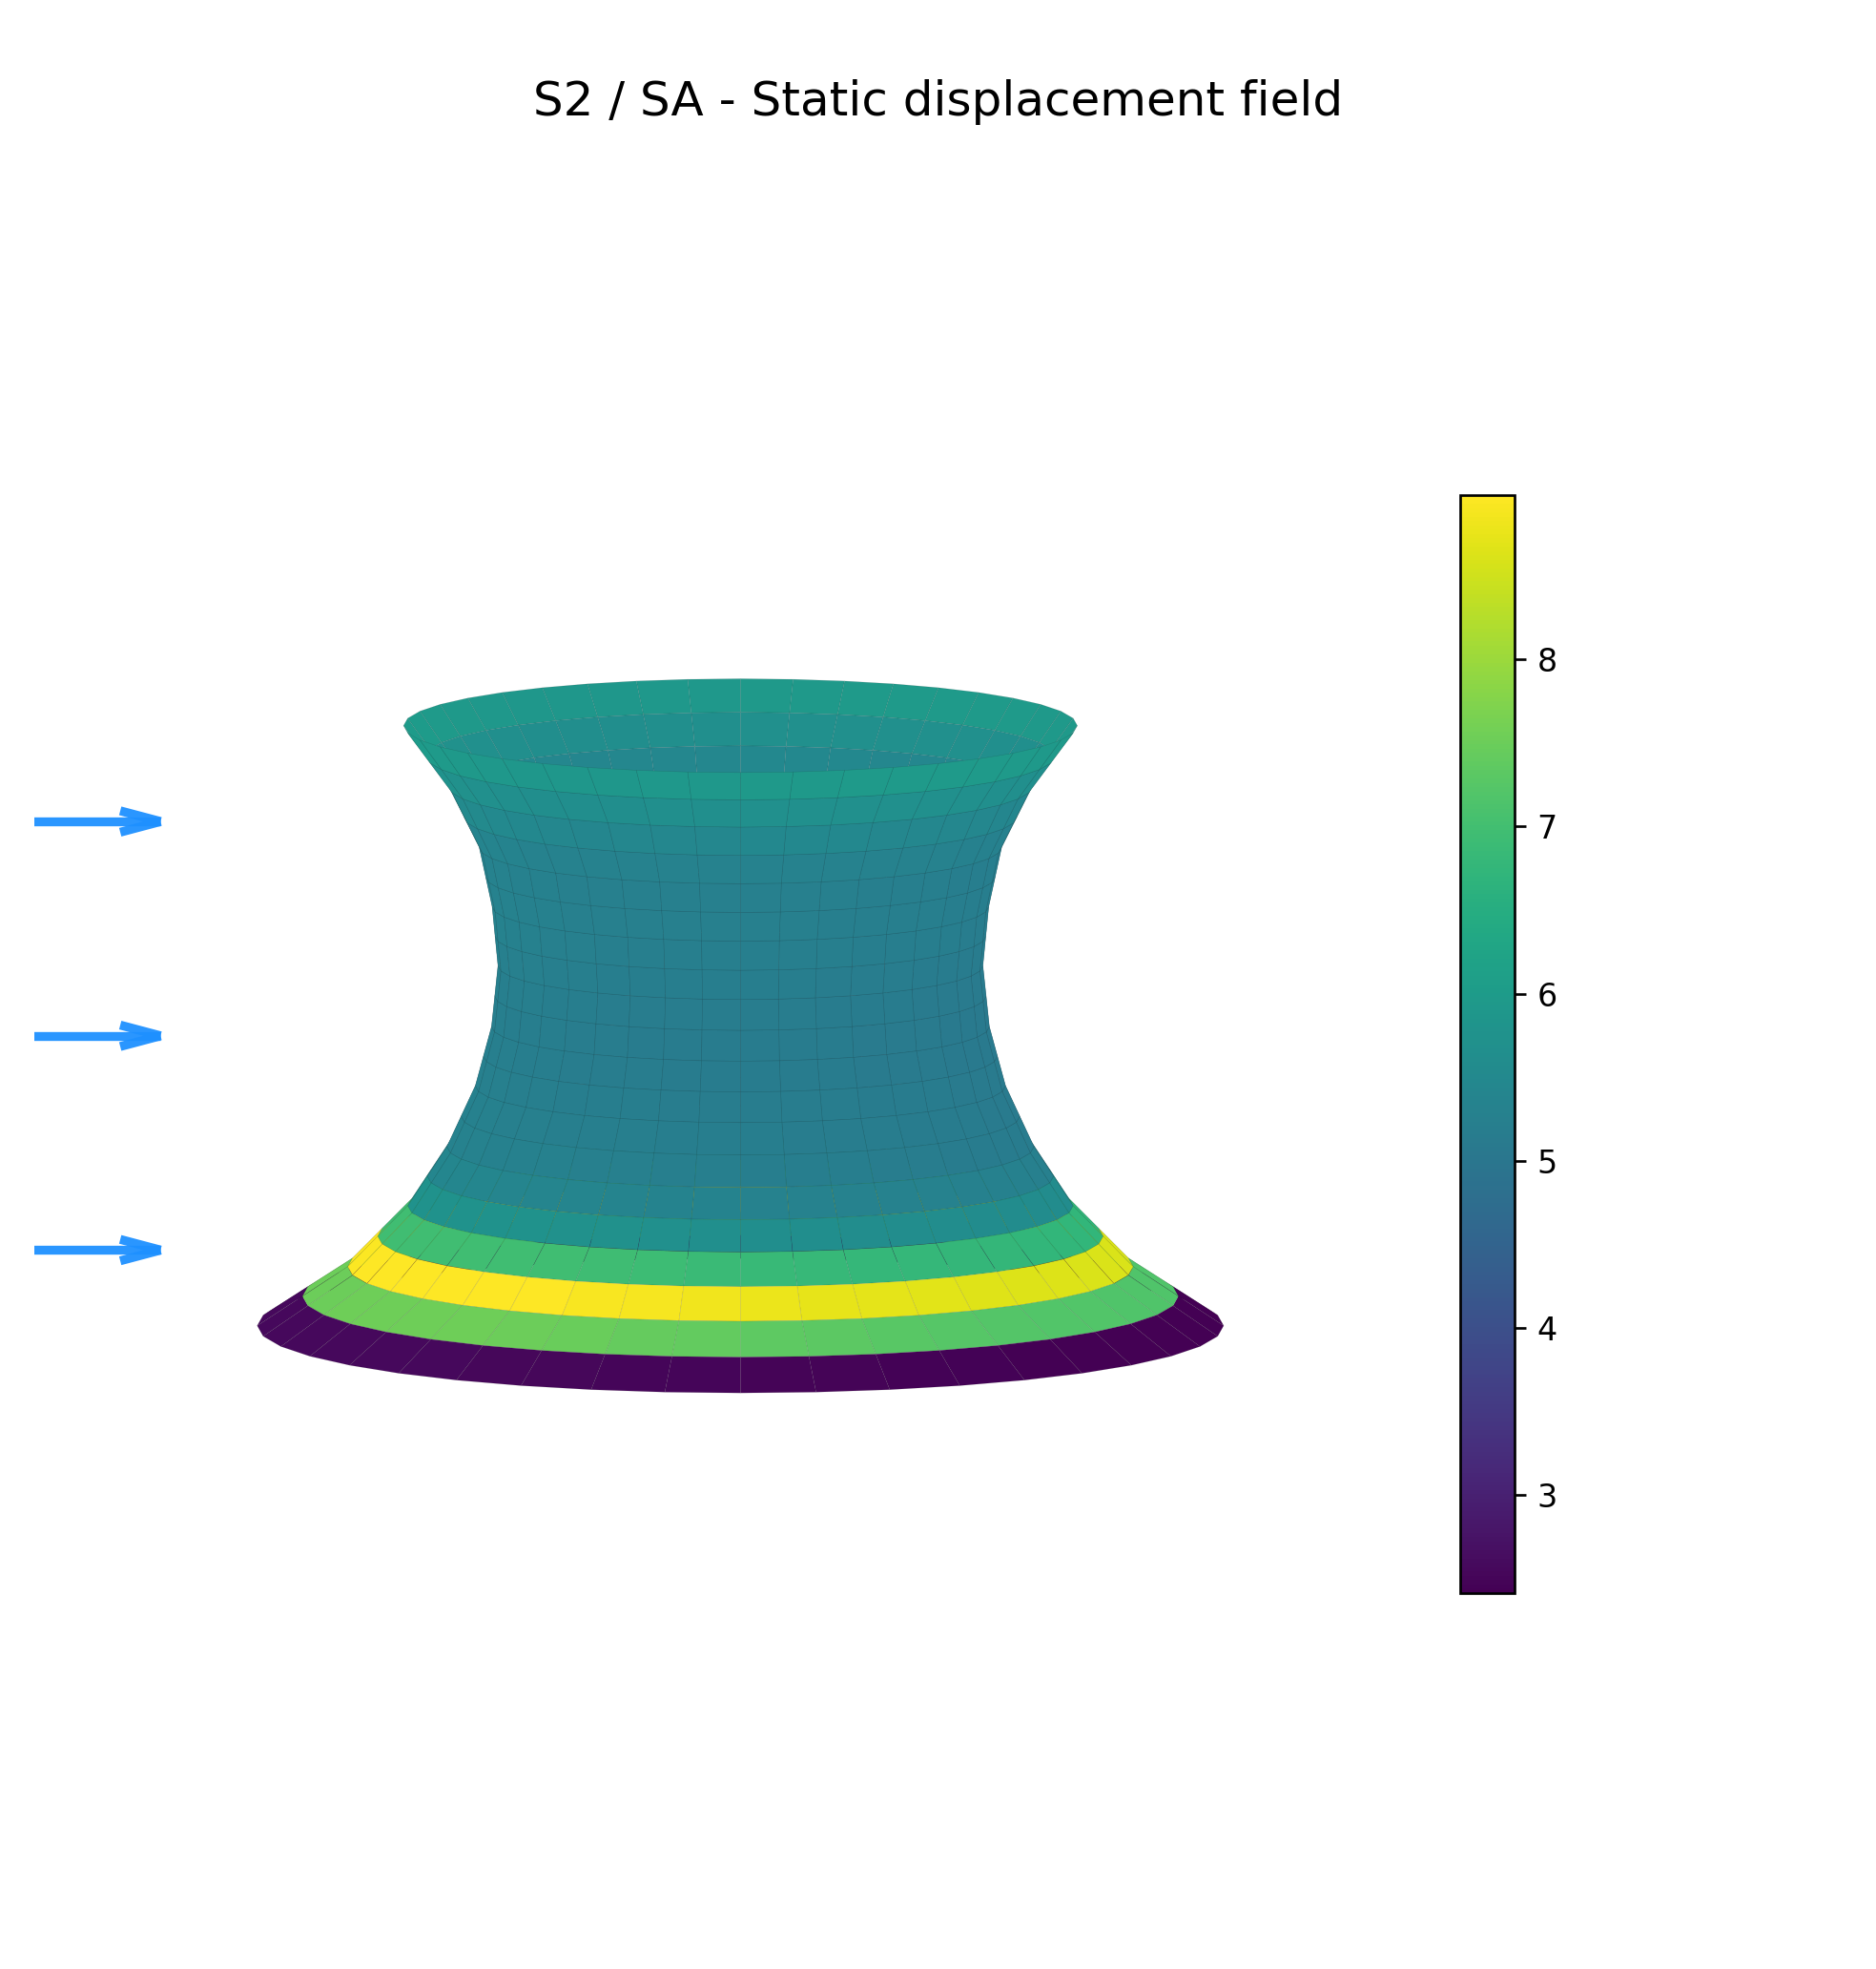
\includegraphics[width=\textwidth]{../results/figures/task7_s2_sa_displacement.png}
\caption{S2 / SA displacement}
\end{subfigure}\hfill
\begin{subfigure}{0.32\textwidth}
\centering
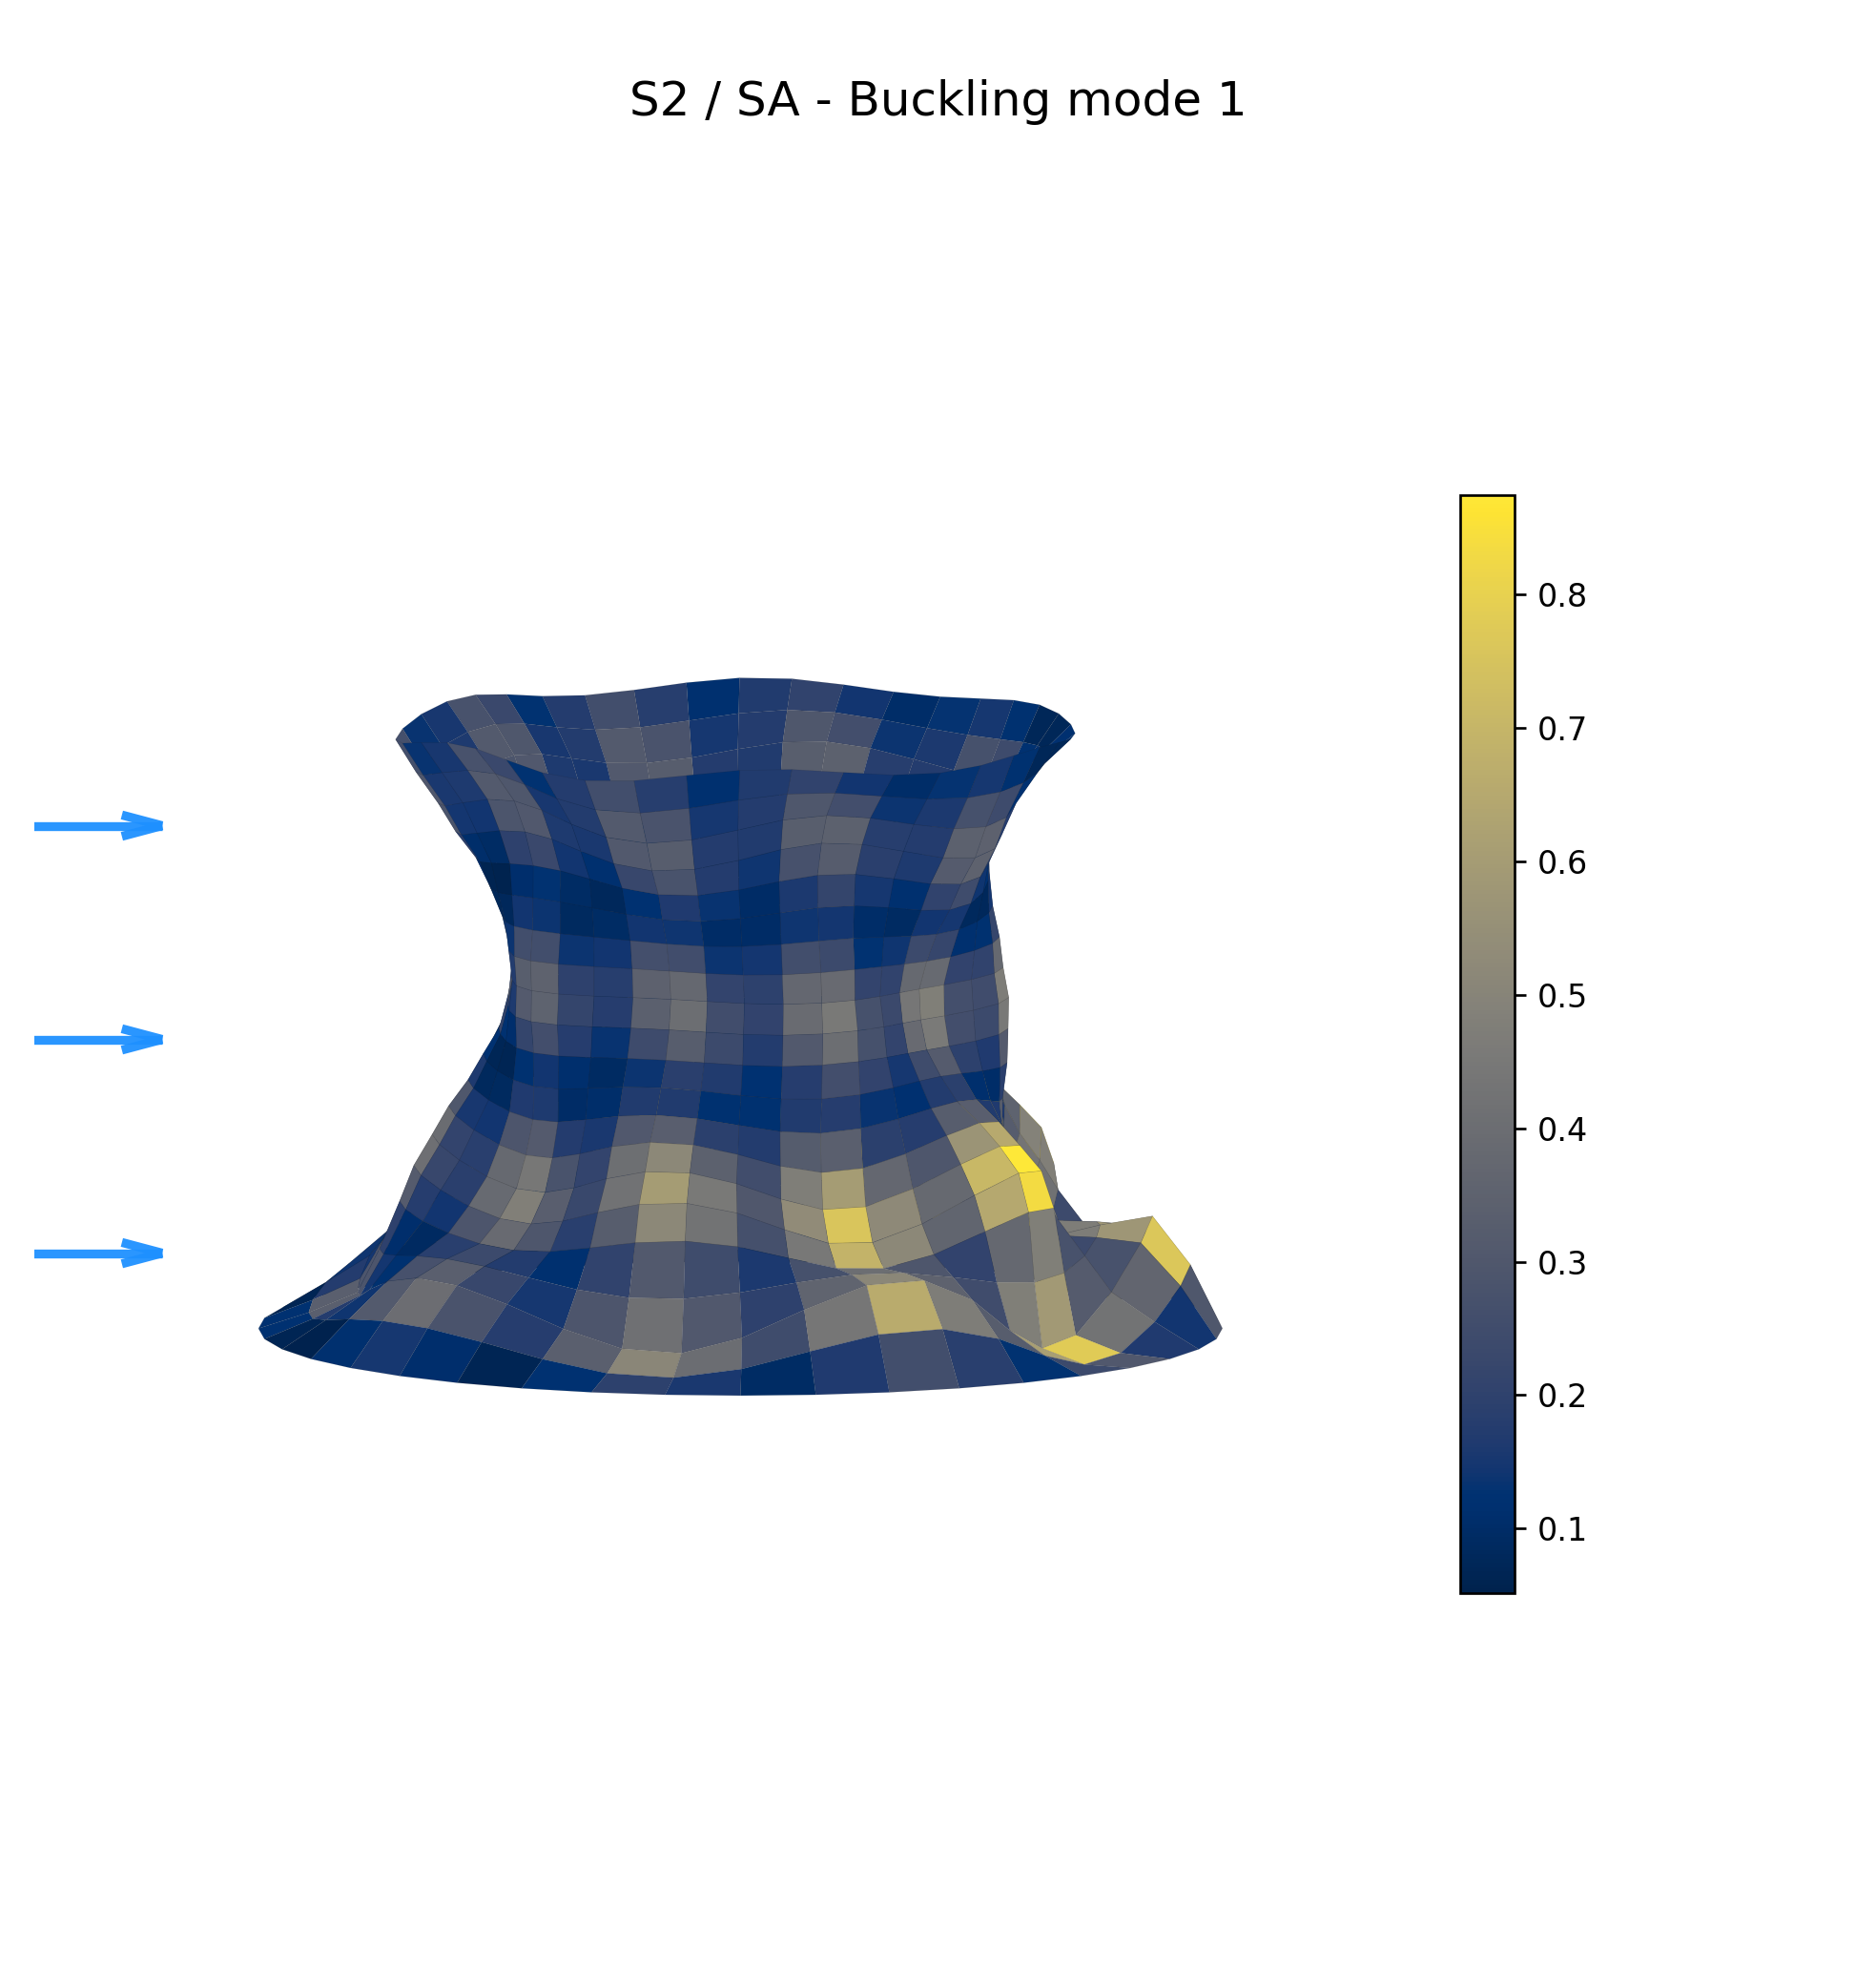
\includegraphics[width=\textwidth]{../results/figures/task7_s2_sa_buckling_mode1.png}
\caption{S2 / SA buckling}
\end{subfigure}
\caption{Combined visual fields}
\end{figure}


\noindent \textbf{Performance Discussion (Rank 3):} The \texttt{S2 / SA} model (Engineering-feasible) achieved an overall weighted score of \texttt{7.500}. It demonstrates strong structural integrity with a first buckling factor of \texttt{24.549}. Under the applied wind load, the maximum observed displacement is bounded at \texttt{9.968 mm}, and peak von Mises stresses reach \texttt{3.818 MPa}. As a high-ranking runner-up, it presents an extremely competitive alternative, trading minimal surface area differences for robust stress and displacement behavior.


\section{S3 / PSO}


\begin{figure}[H]
\centering
\begin{subfigure}{0.32\textwidth}
\centering
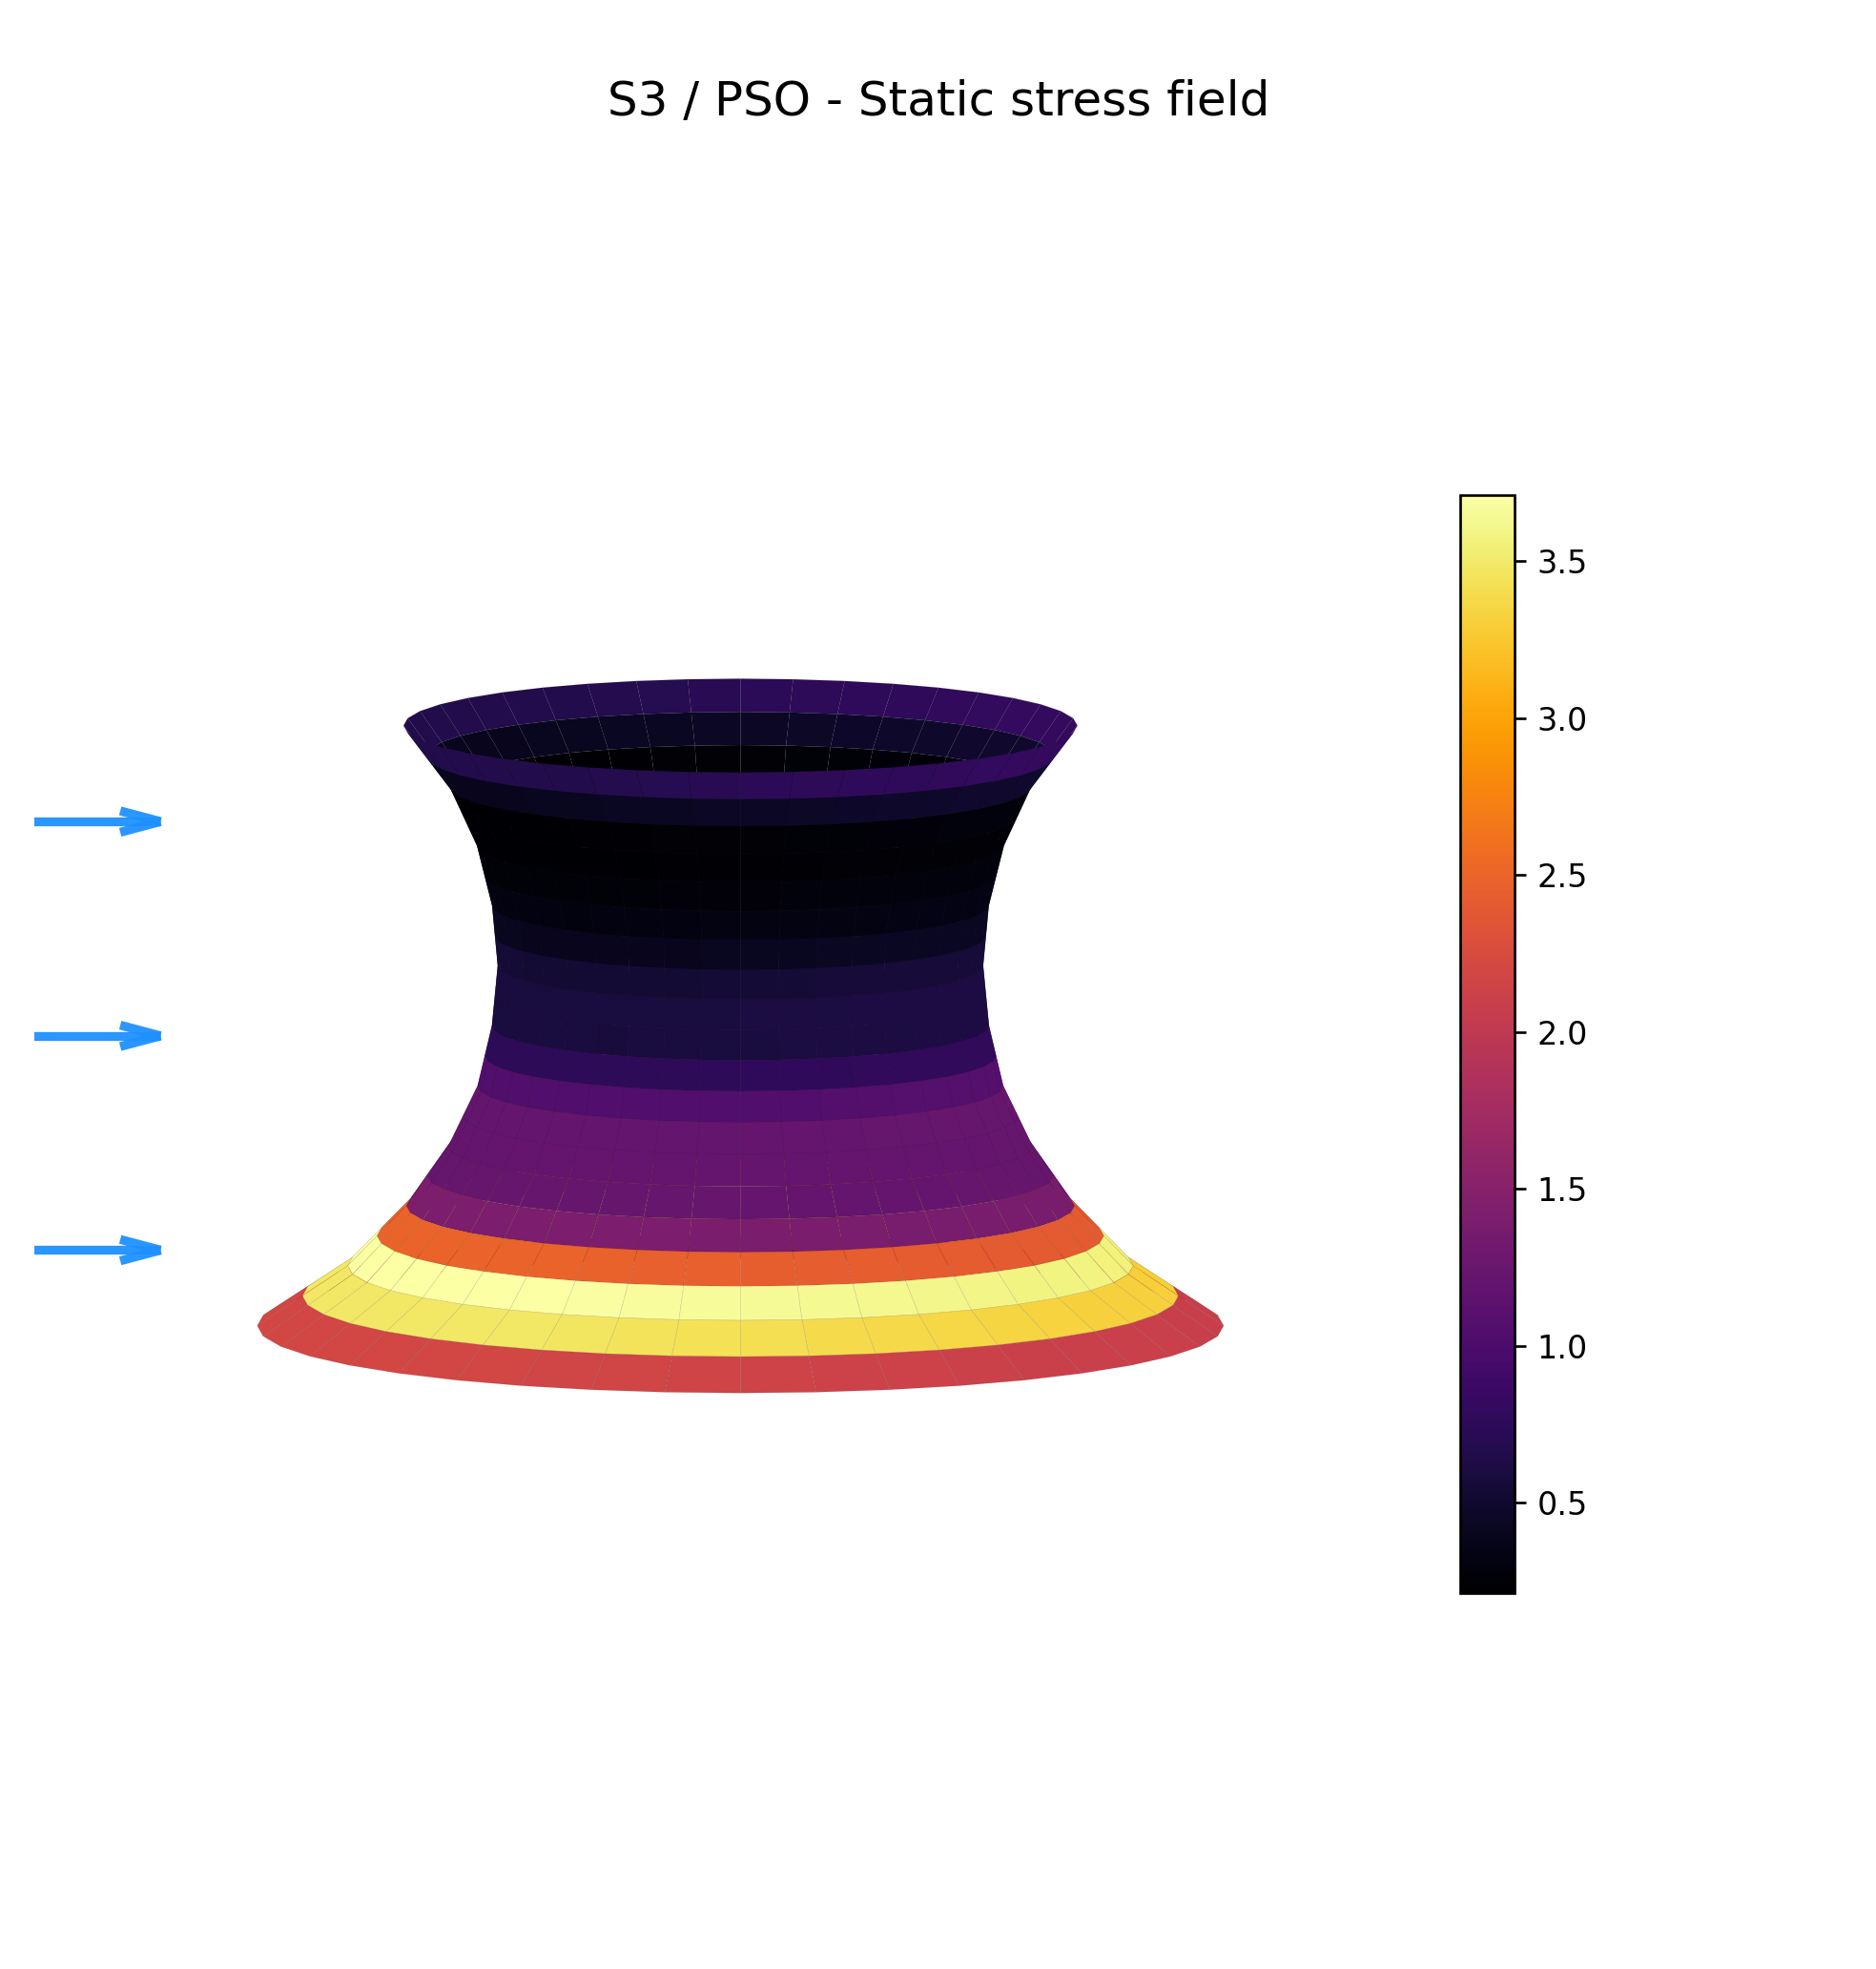
\includegraphics[width=\textwidth]{../results/figures/task7_s3_pso_stress.png}
\caption{S3 / PSO stress}
\end{subfigure}\hfill
\begin{subfigure}{0.32\textwidth}
\centering
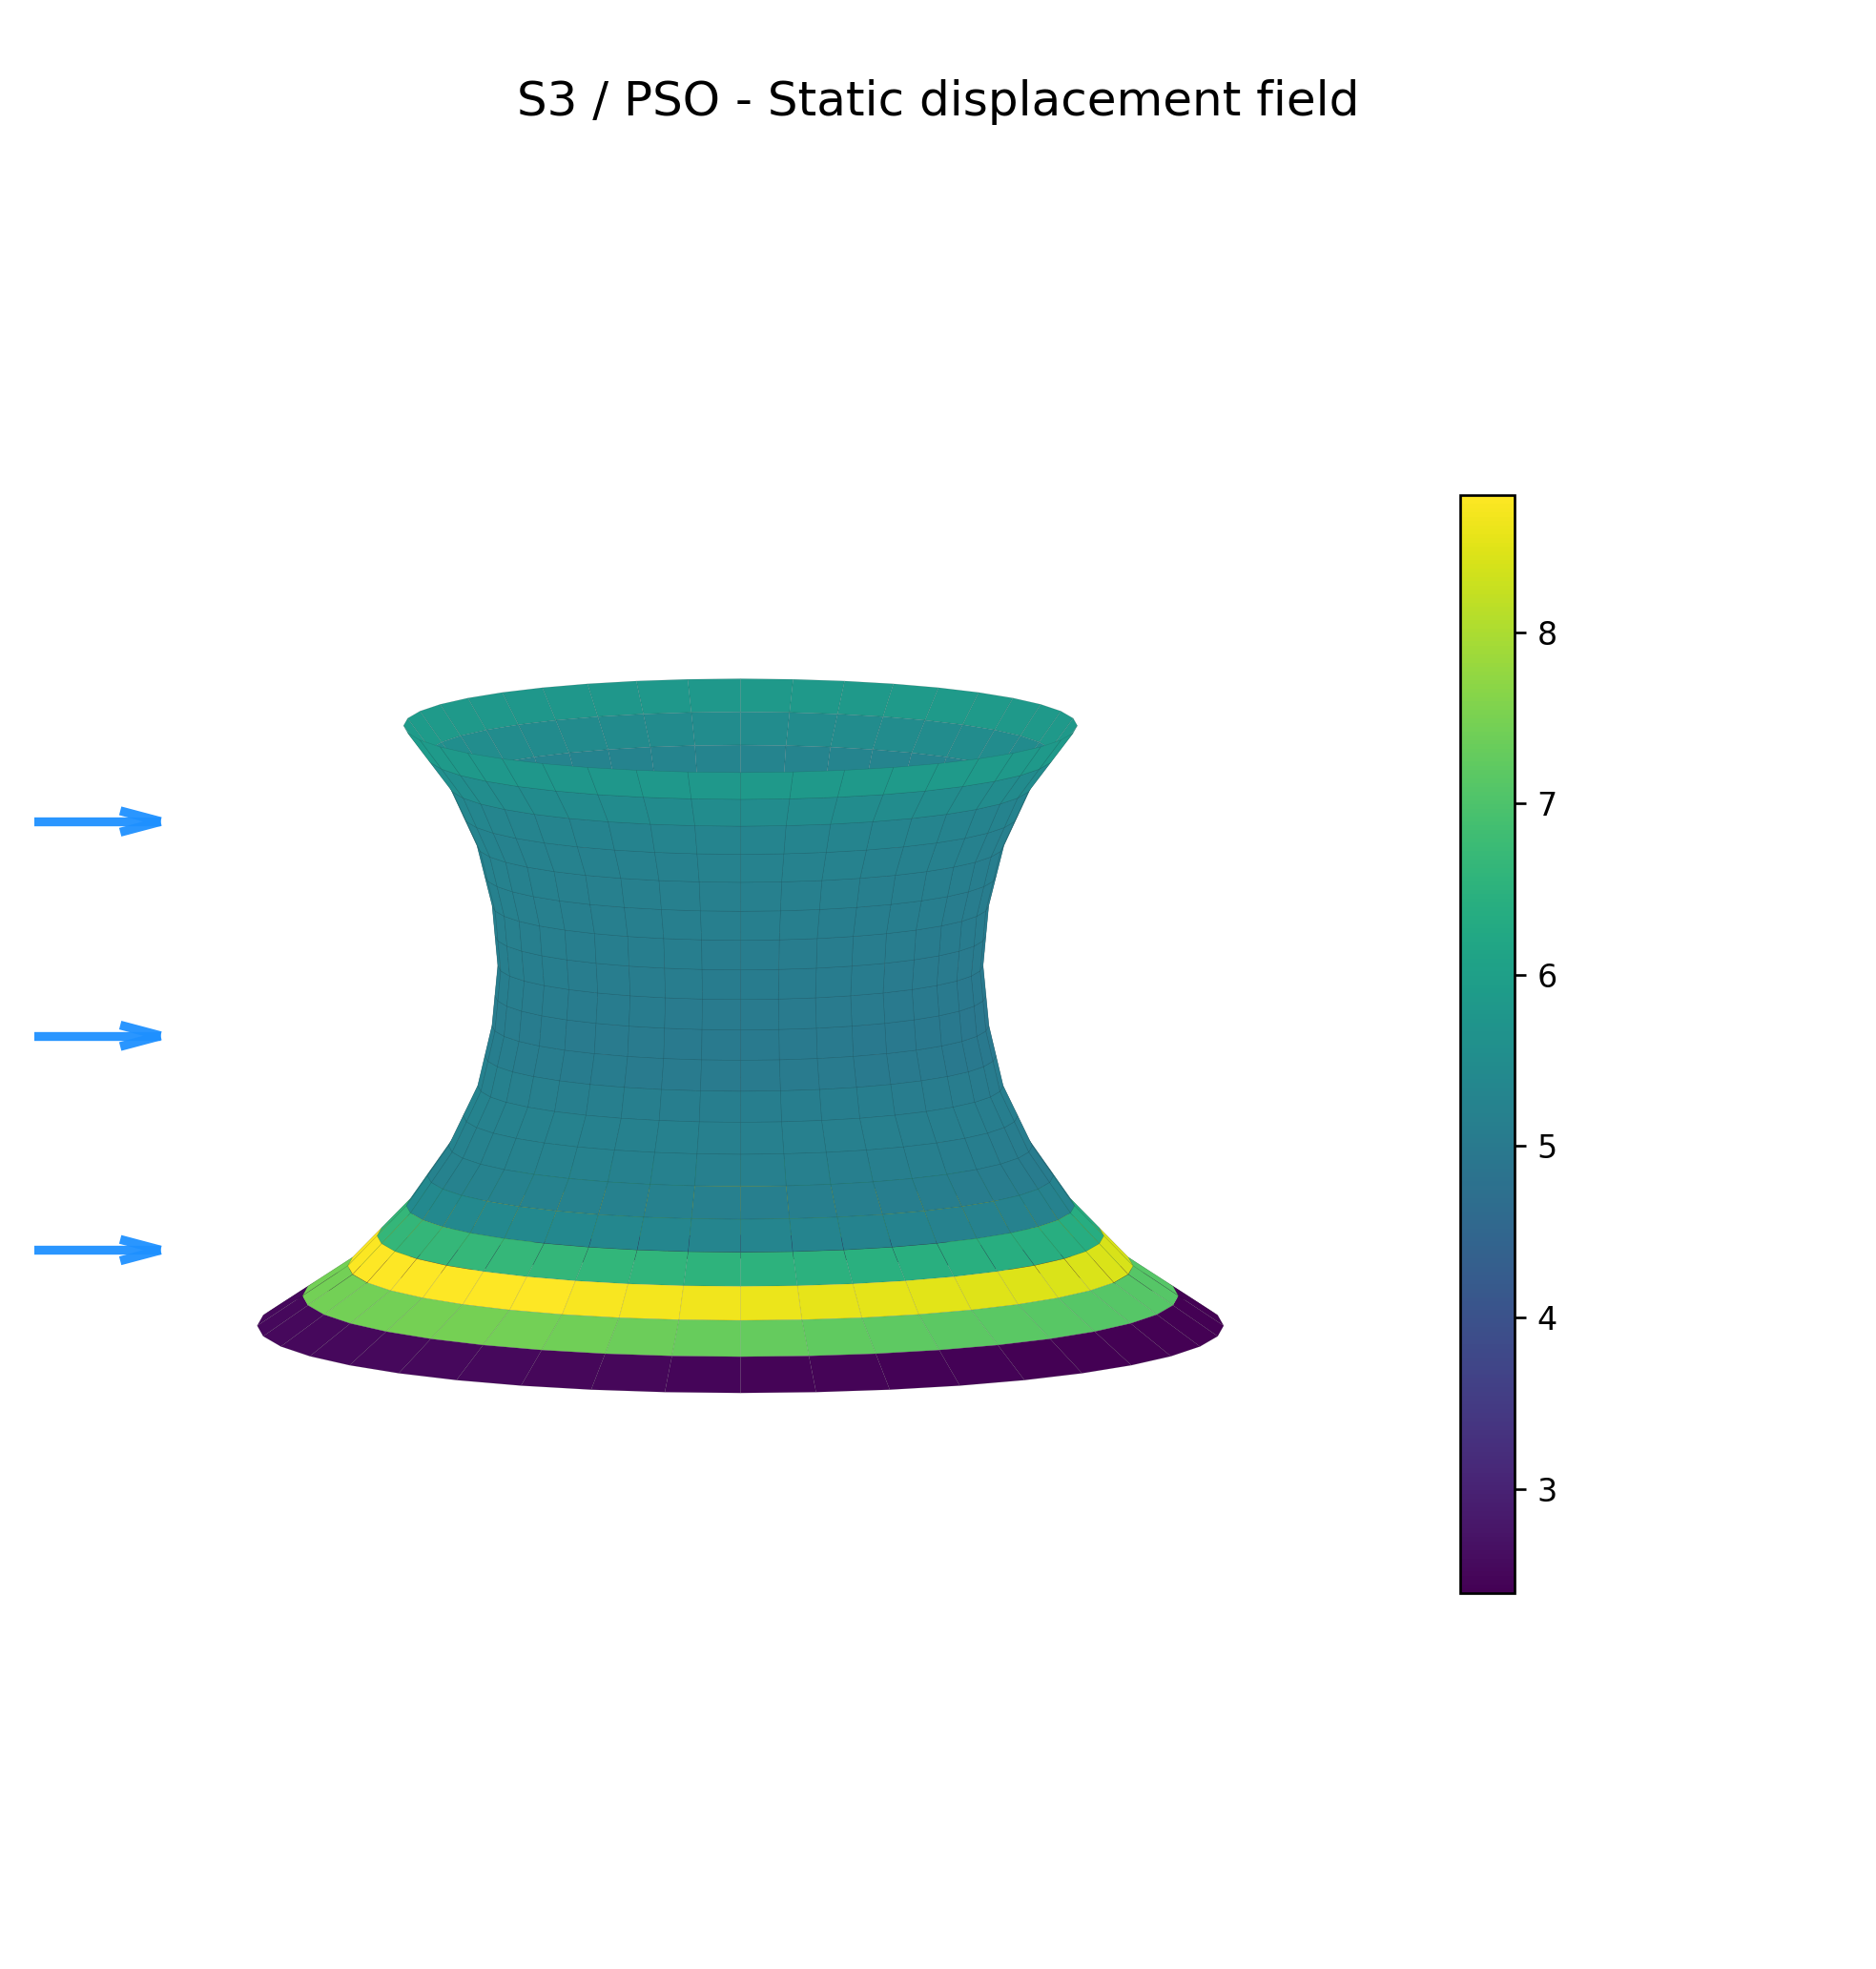
\includegraphics[width=\textwidth]{../results/figures/task7_s3_pso_displacement.png}
\caption{S3 / PSO displacement}
\end{subfigure}\hfill
\begin{subfigure}{0.32\textwidth}
\centering
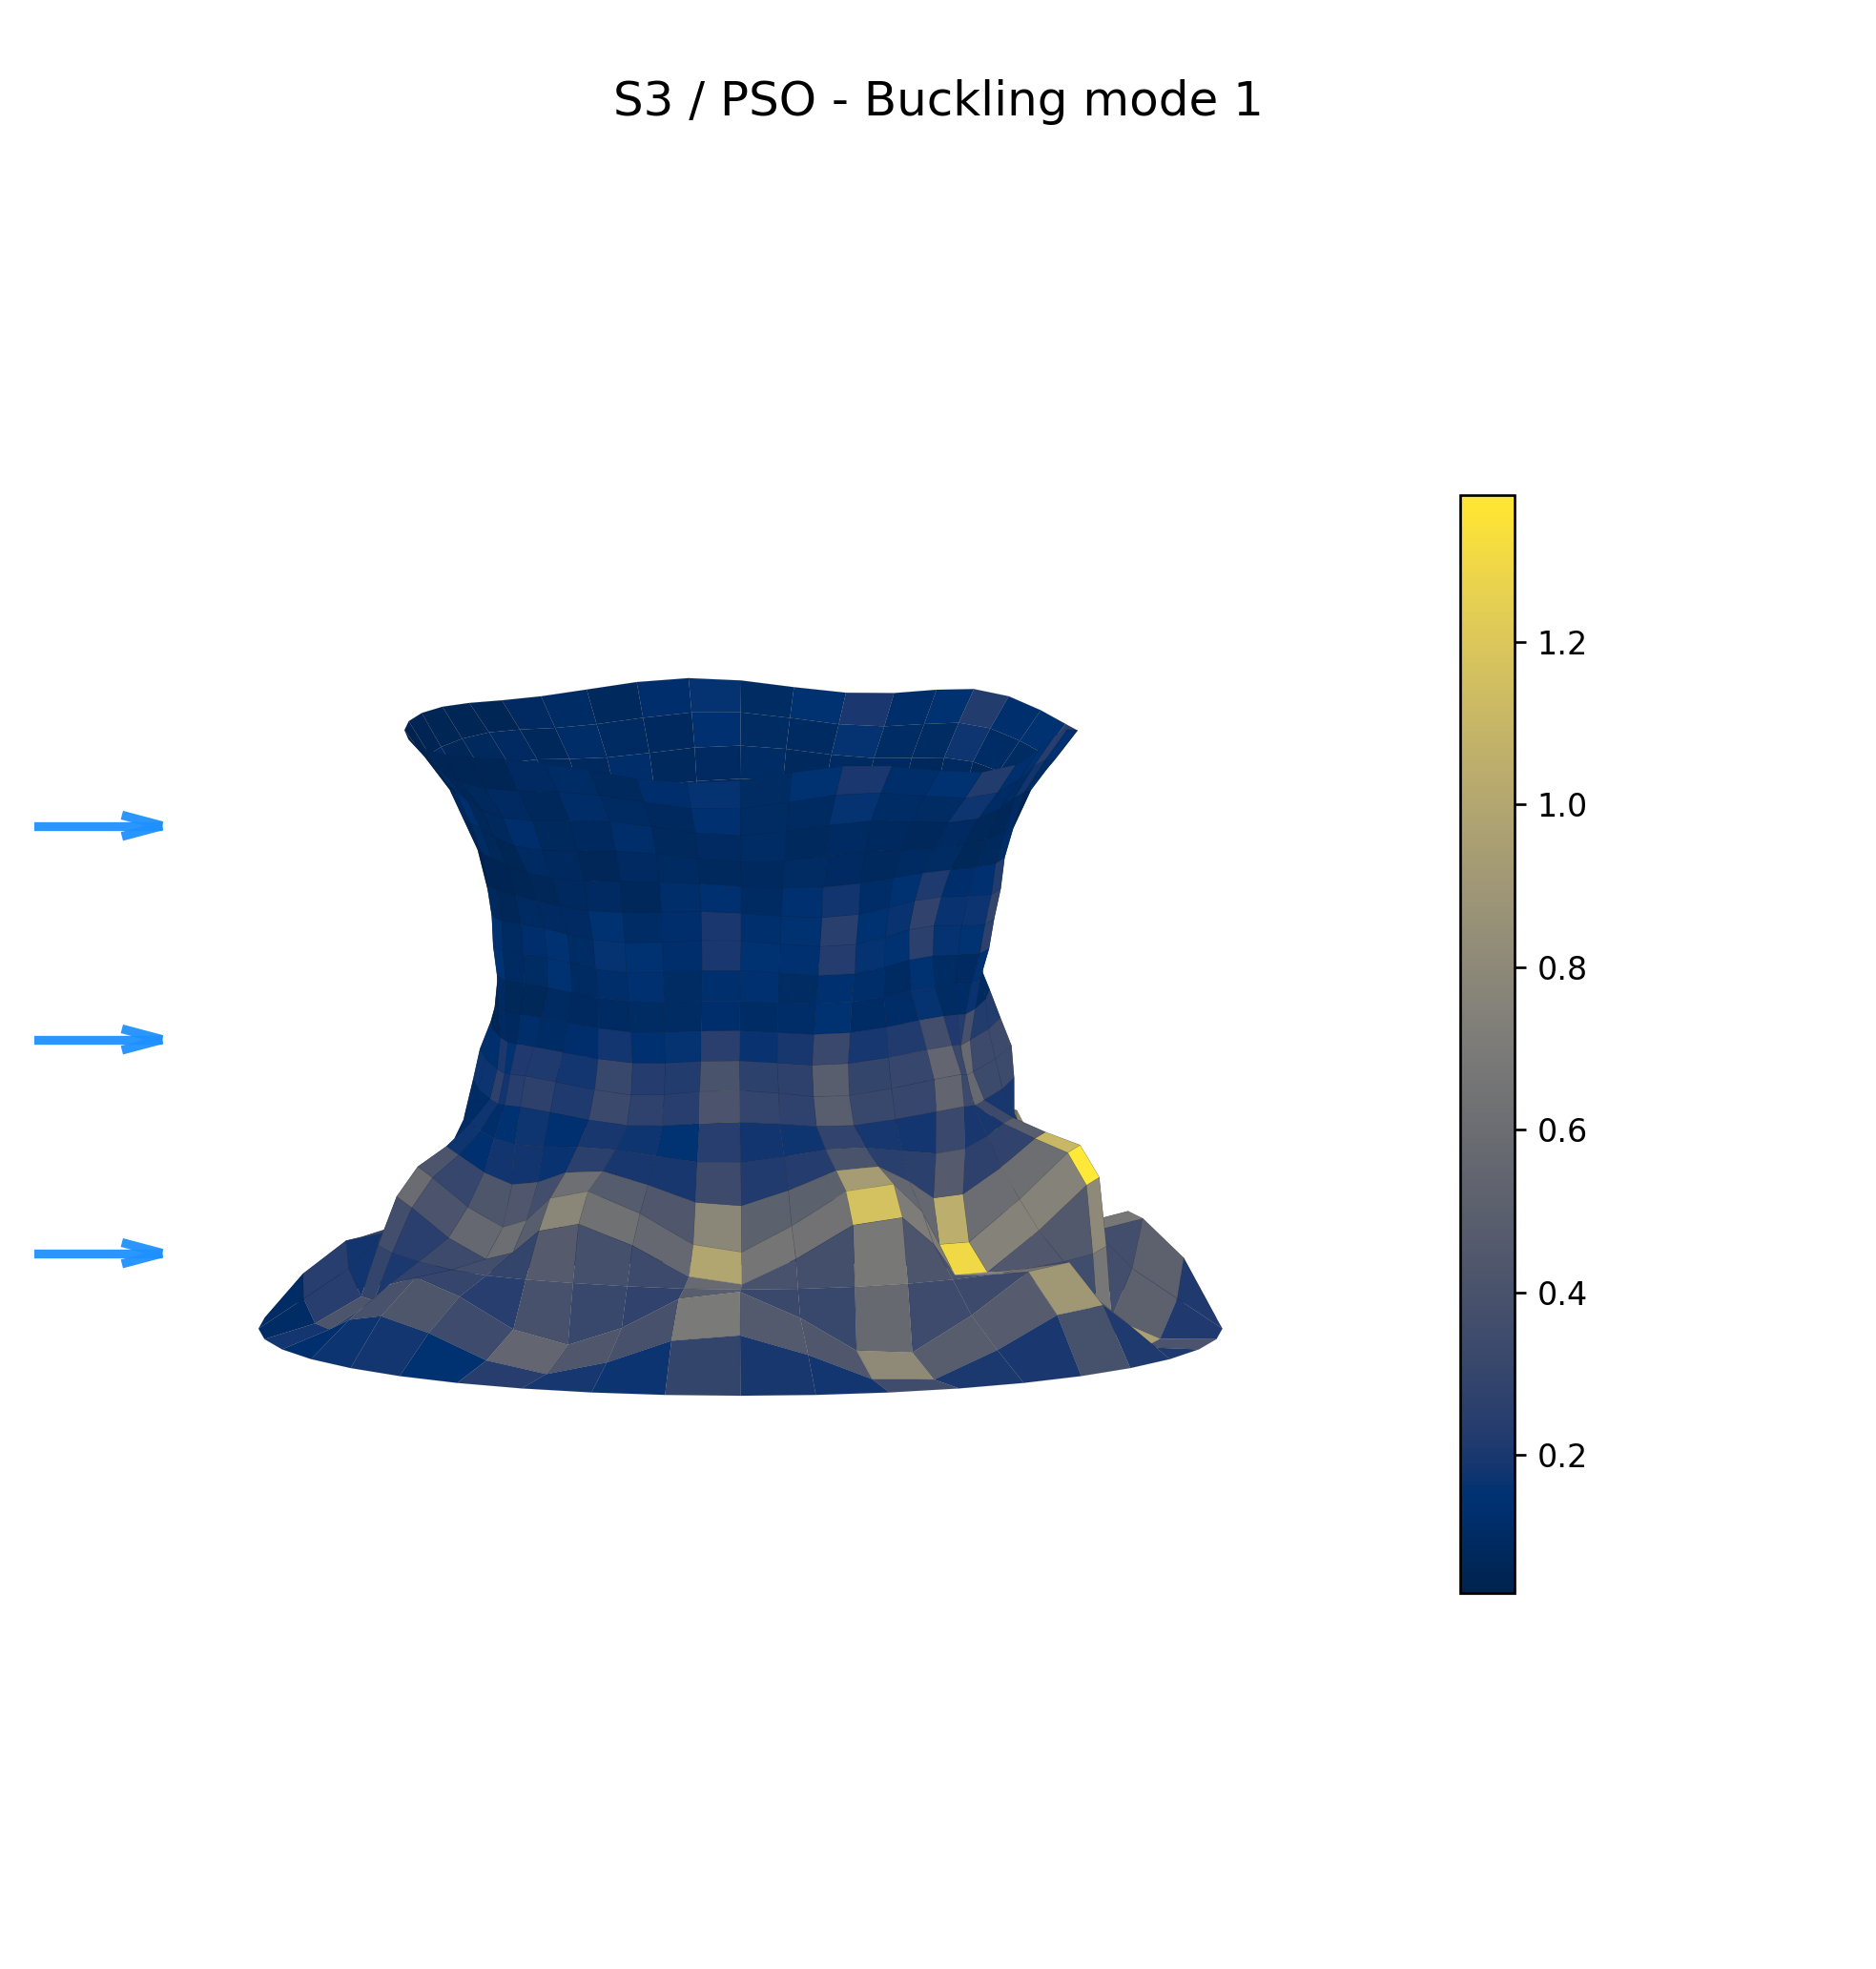
\includegraphics[width=\textwidth]{../results/figures/task7_s3_pso_buckling_mode1.png}
\caption{S3 / PSO buckling}
\end{subfigure}
\caption{Combined visual fields}
\end{figure}


\noindent \textbf{Performance Discussion (Rank 4):} The \texttt{S3 / PSO} model (Engineering-feasible) achieved an overall weighted score of \texttt{9.650}. It demonstrates strong structural integrity with a first buckling factor of \texttt{23.496}. Under the applied wind load, the maximum observed displacement is bounded at \texttt{9.850 mm}, and peak von Mises stresses reach \texttt{3.794 MPa}. Although ranking slightly lower within the top 5, it remains a structurally sound and convincing concept that safely satisfies engineering constraints.


\section{S2 / BFGS}


\begin{figure}[H]
\centering
\begin{subfigure}{0.32\textwidth}
\centering
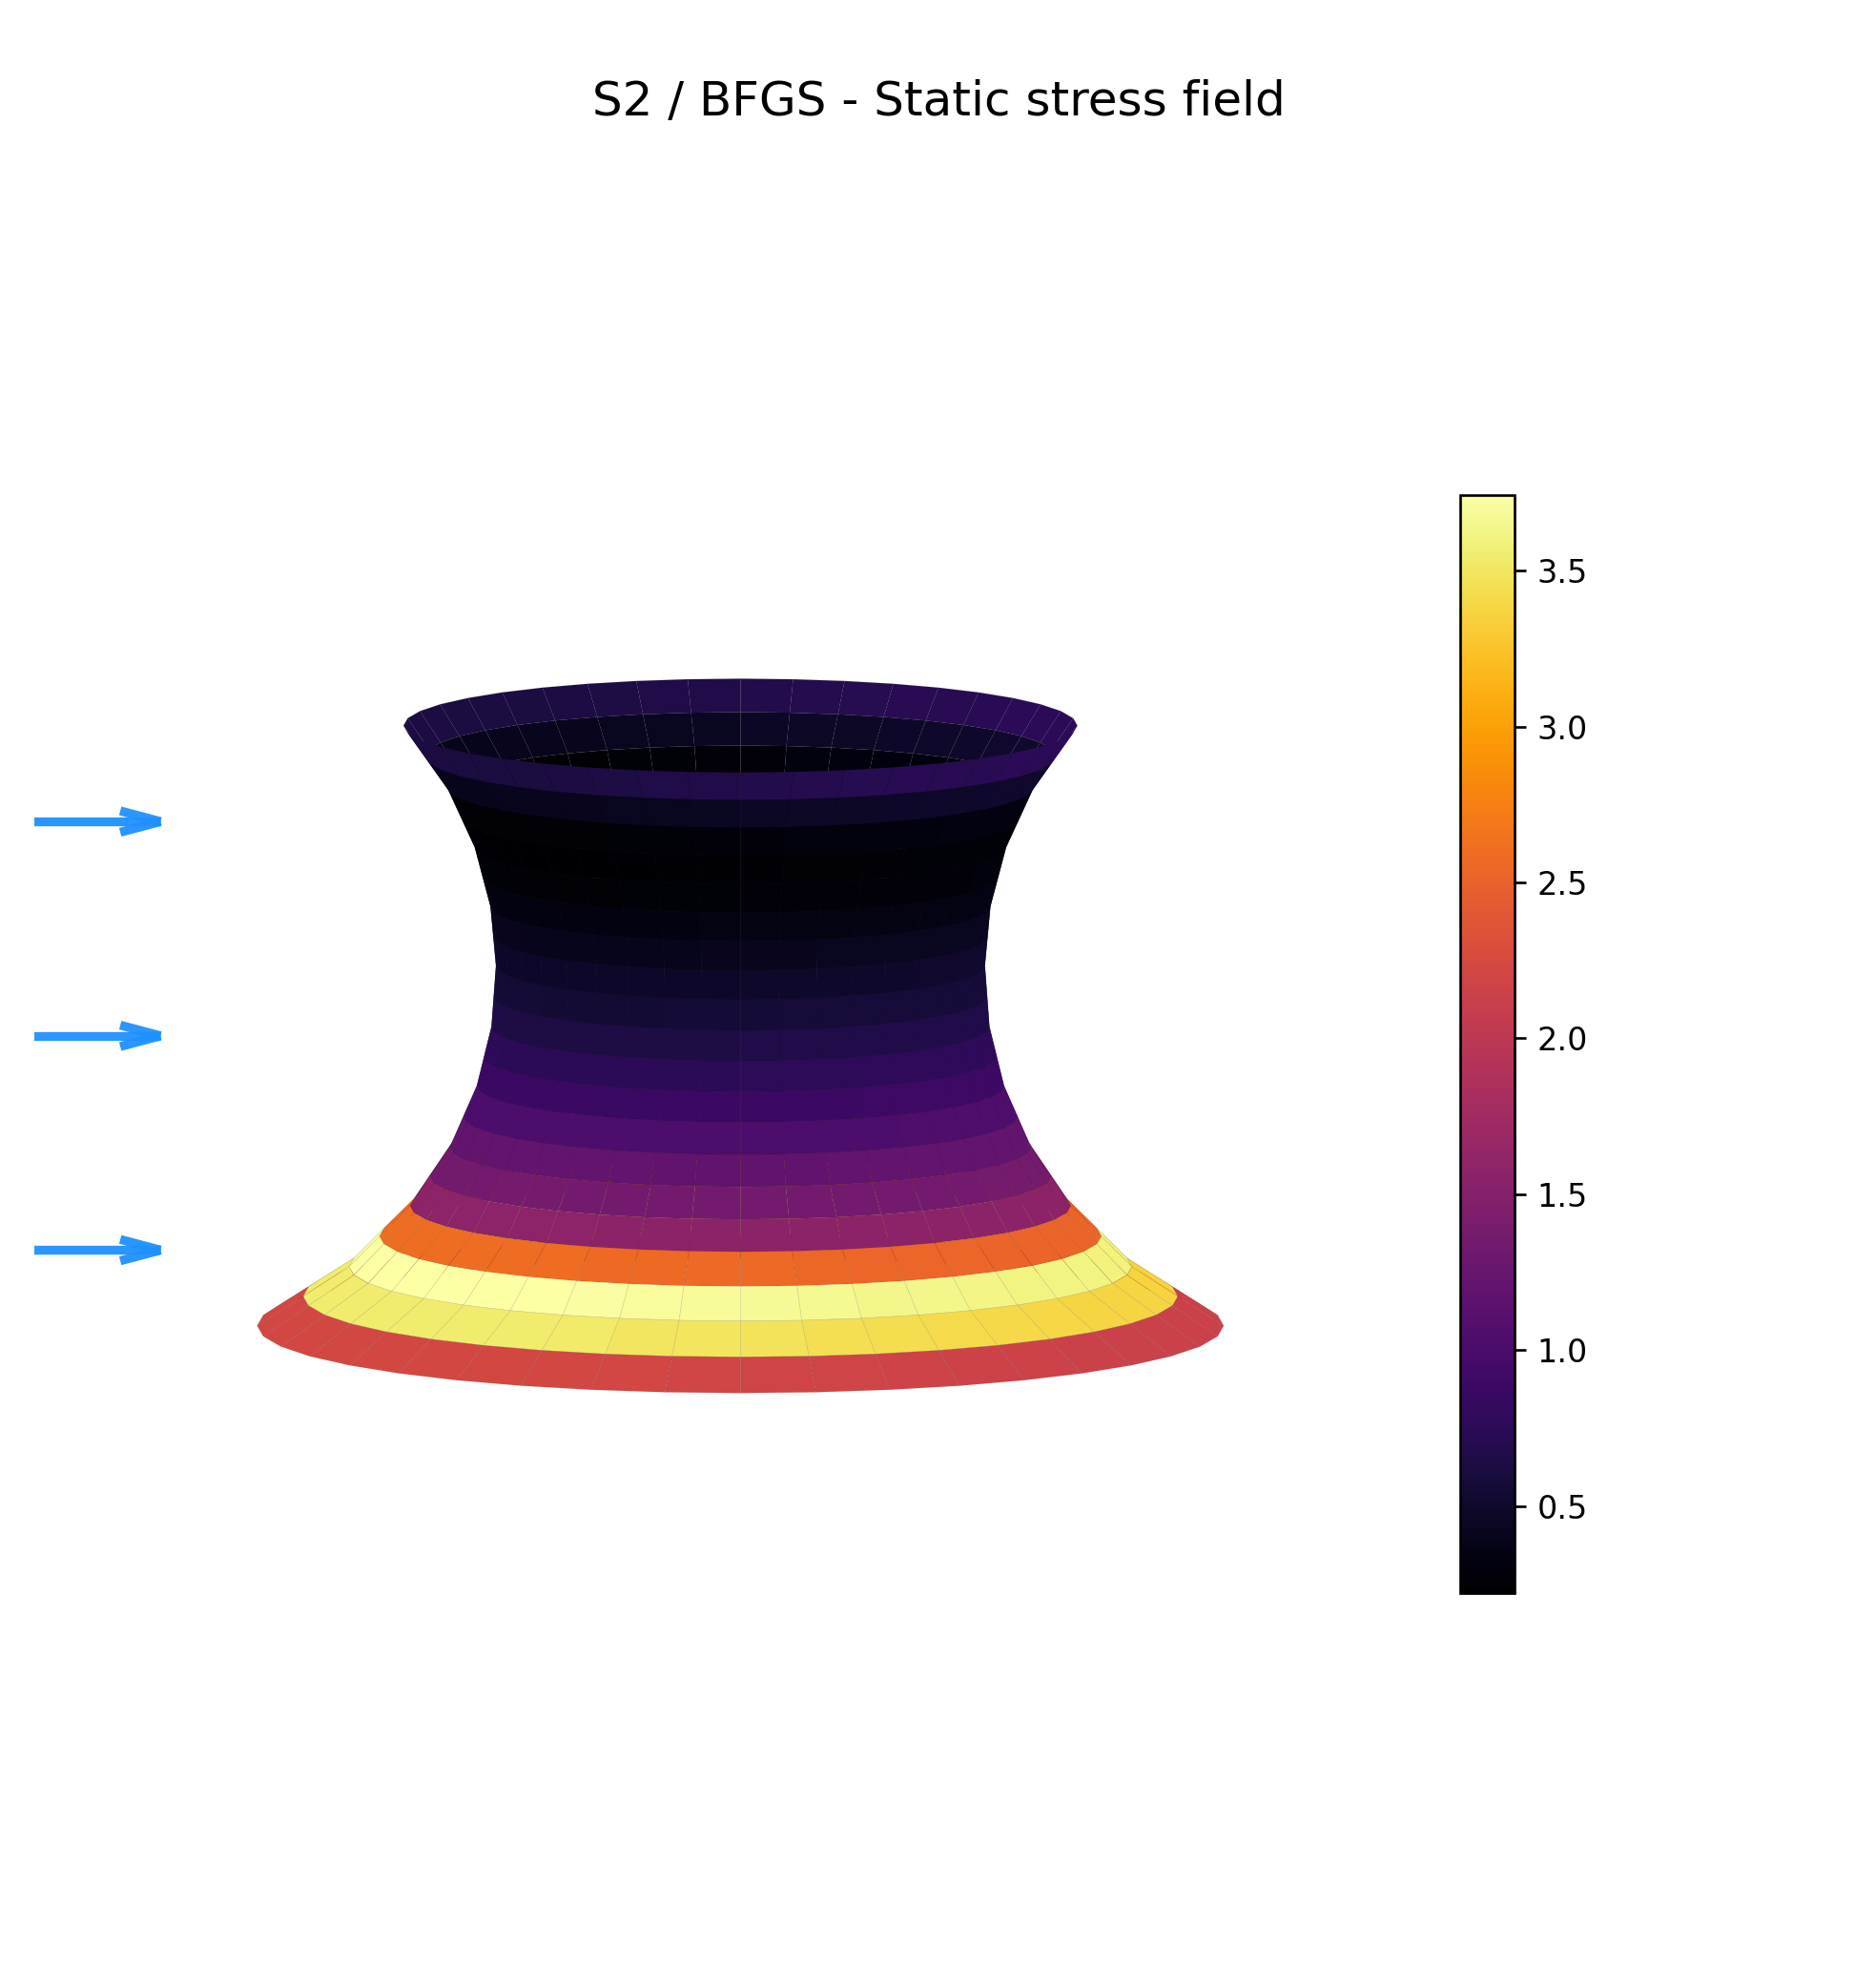
\includegraphics[width=\textwidth]{../results/figures/task7_s2_bfgs_stress.png}
\caption{S2 / BFGS stress}
\end{subfigure}\hfill
\begin{subfigure}{0.32\textwidth}
\centering
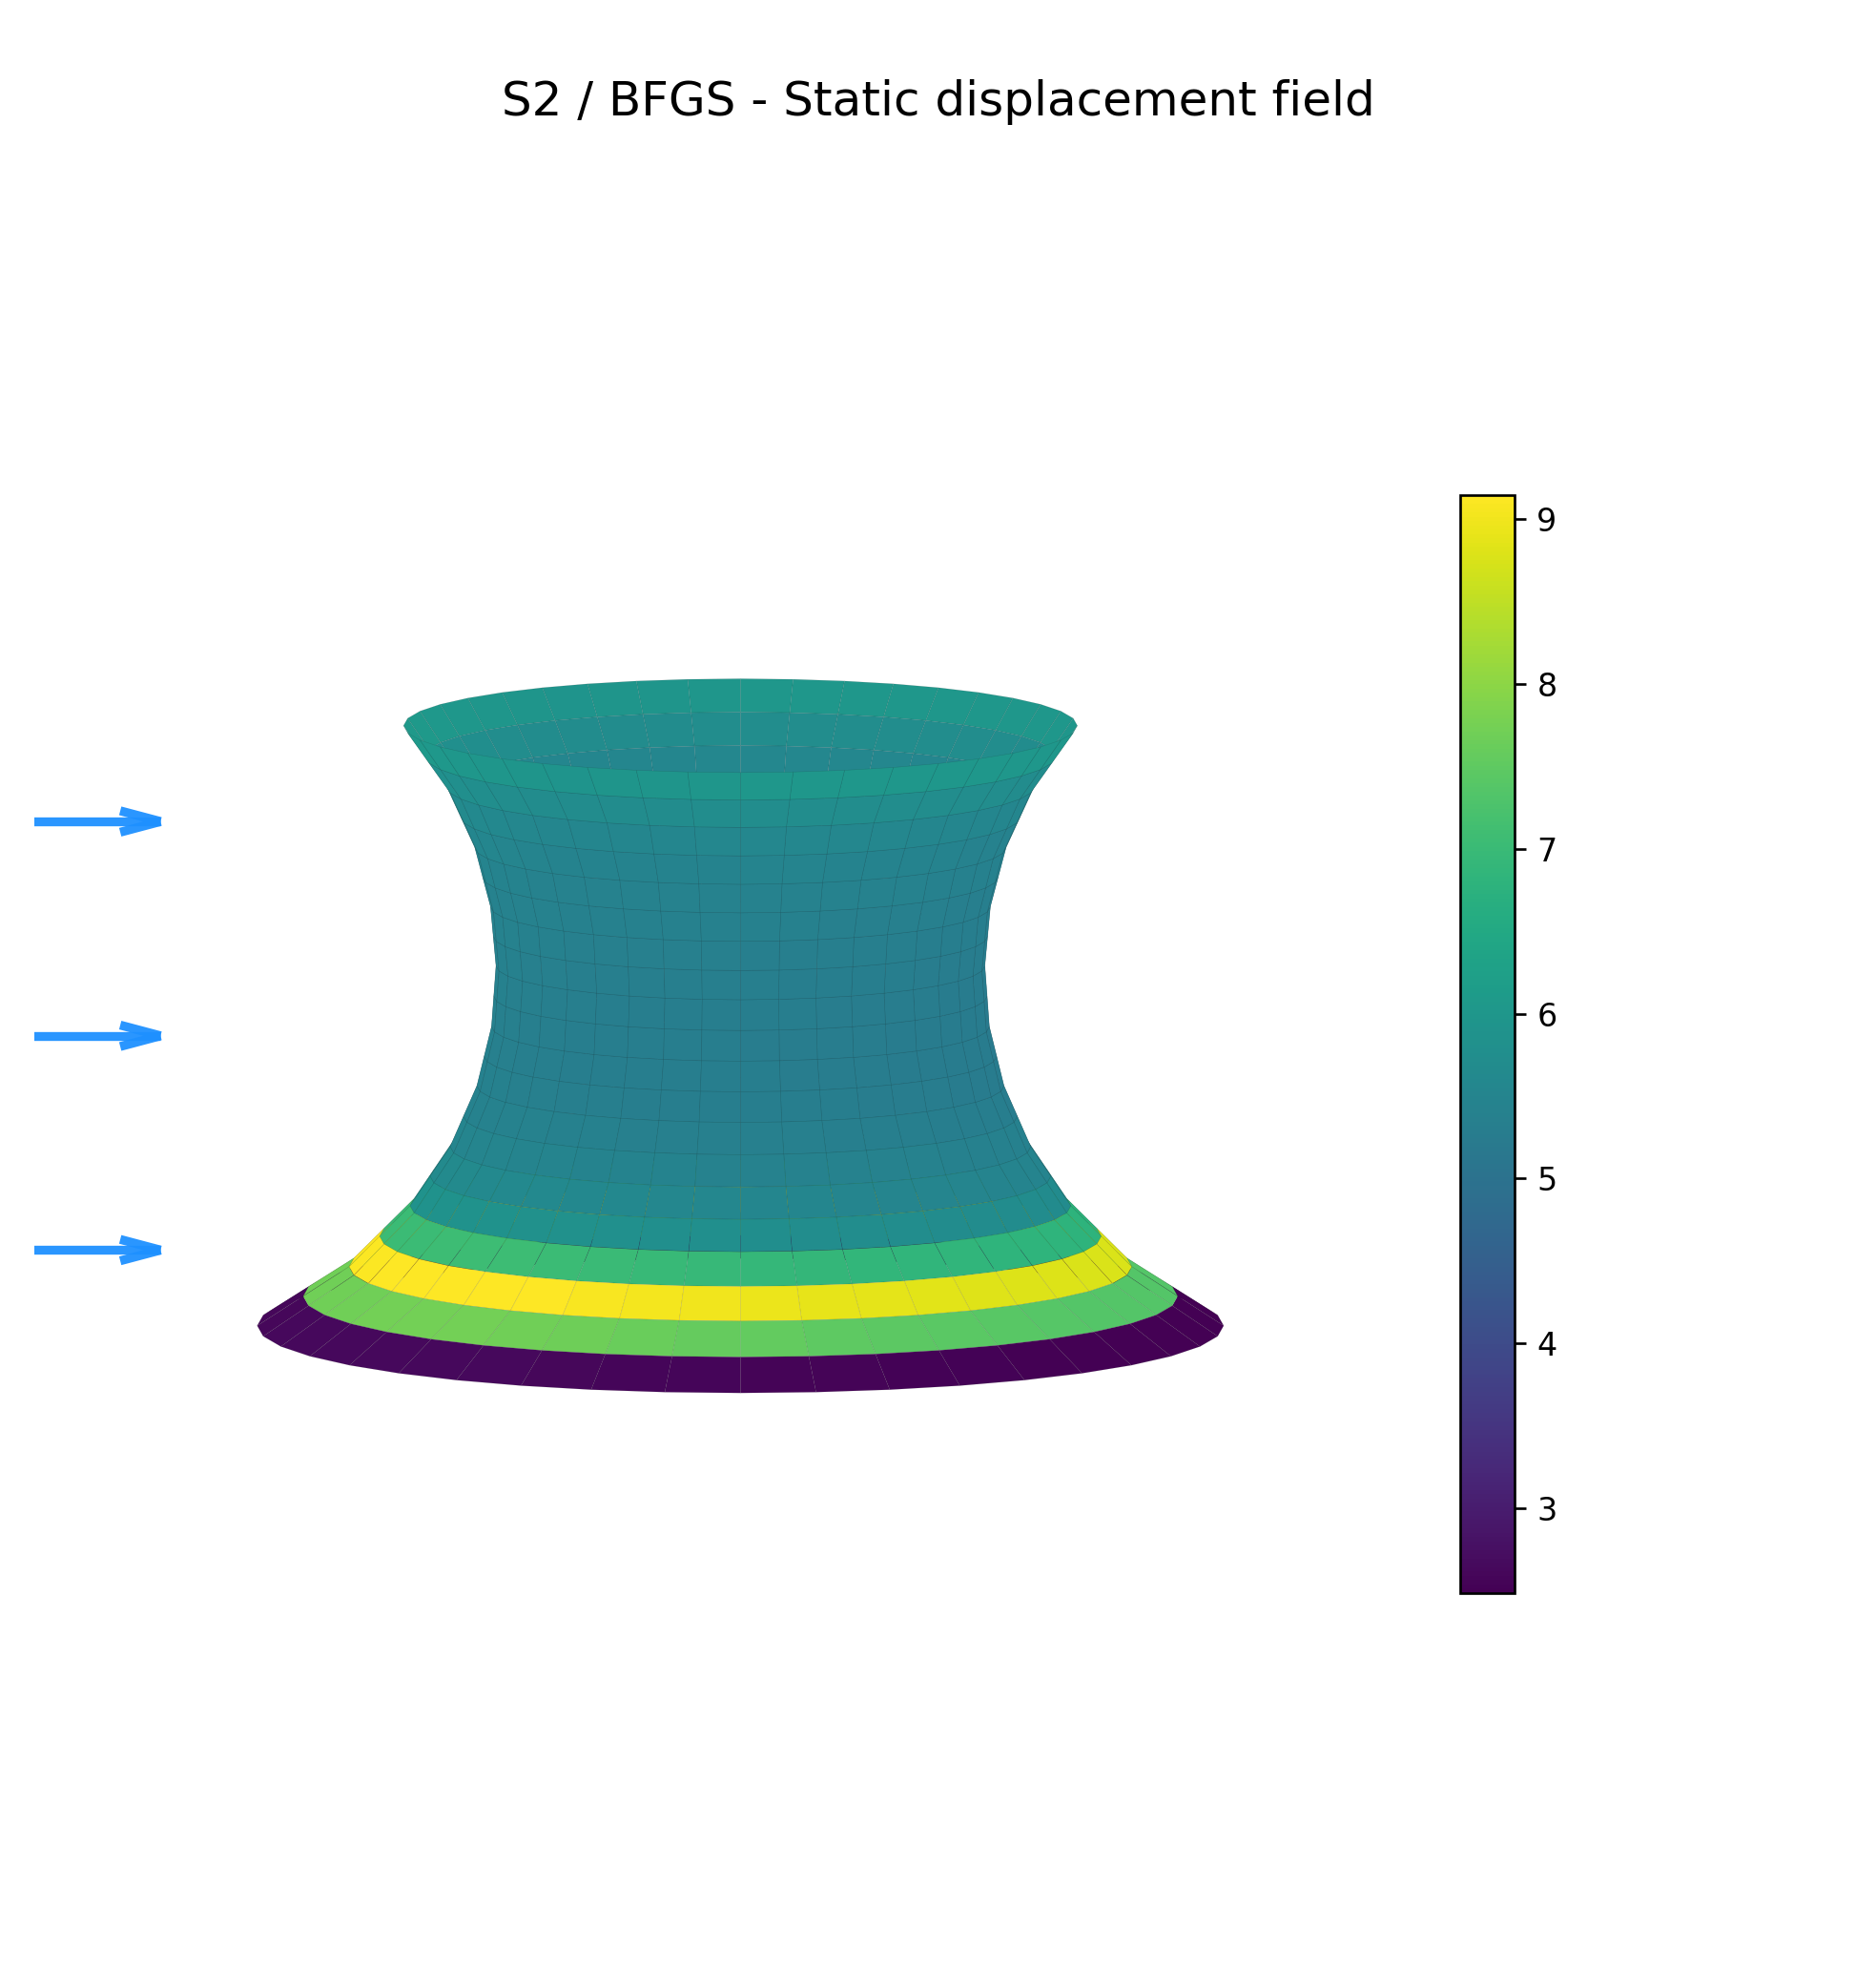
\includegraphics[width=\textwidth]{../results/figures/task7_s2_bfgs_displacement.png}
\caption{S2 / BFGS displacement}
\end{subfigure}\hfill
\begin{subfigure}{0.32\textwidth}
\centering
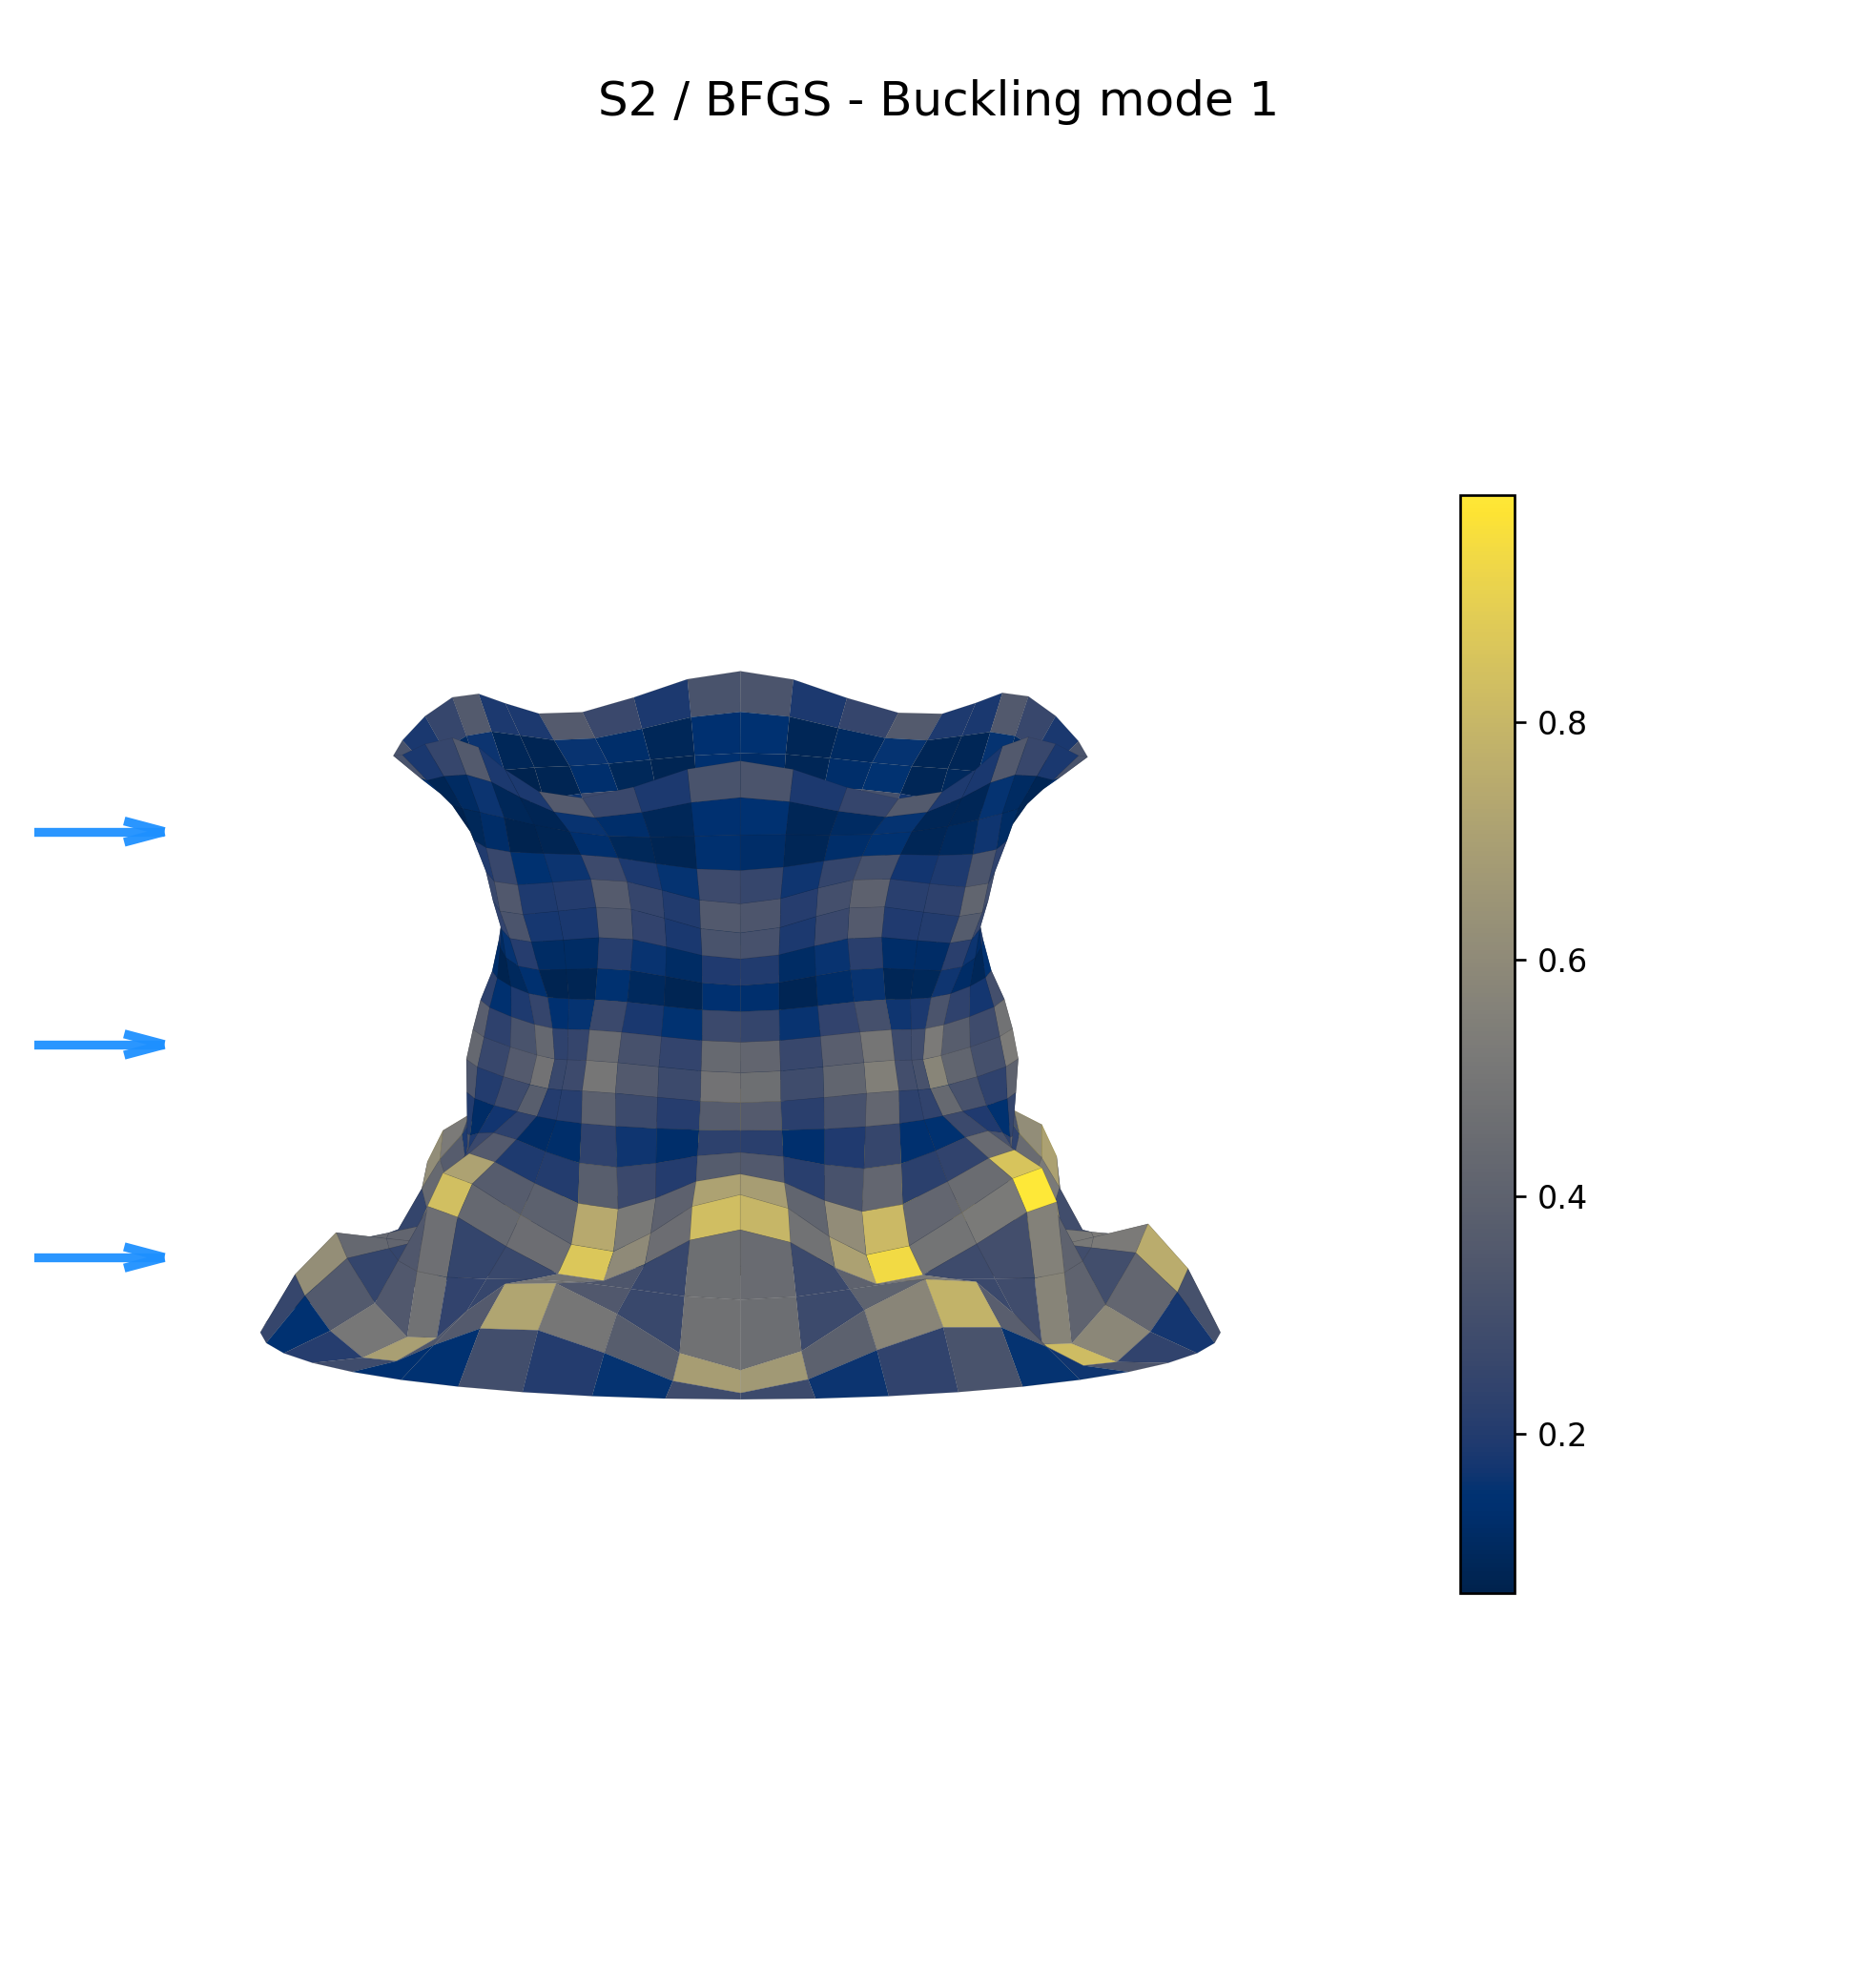
\includegraphics[width=\textwidth]{../results/figures/task7_s2_bfgs_buckling_mode1.png}
\caption{S2 / BFGS buckling}
\end{subfigure}
\caption{Combined visual fields}
\end{figure}


\noindent \textbf{Performance Discussion (Rank 5):} The \texttt{S2 / BFGS} model (Engineering-feasible) achieved an overall weighted score of \texttt{9.850}. It demonstrates strong structural integrity with a first buckling factor of \texttt{23.563}. Under the applied wind load, the maximum observed displacement is bounded at \texttt{10.202 mm}, and peak von Mises stresses reach \texttt{3.867 MPa}. Although ranking slightly lower within the top 5, it remains a structurally sound and convincing concept that safely satisfies engineering constraints.


\chapter{11. Annex: Complete Field Visualizations}


\noindent This section contains the field visualizations for the remaining 19 candidates out of the total 24 refined presentation models, organized by Scenario.


\section{Scenario S1}


\subsection{S1 / BFGS}


\begin{figure}[H]
\centering
\begin{subfigure}{0.32\textwidth}
\centering
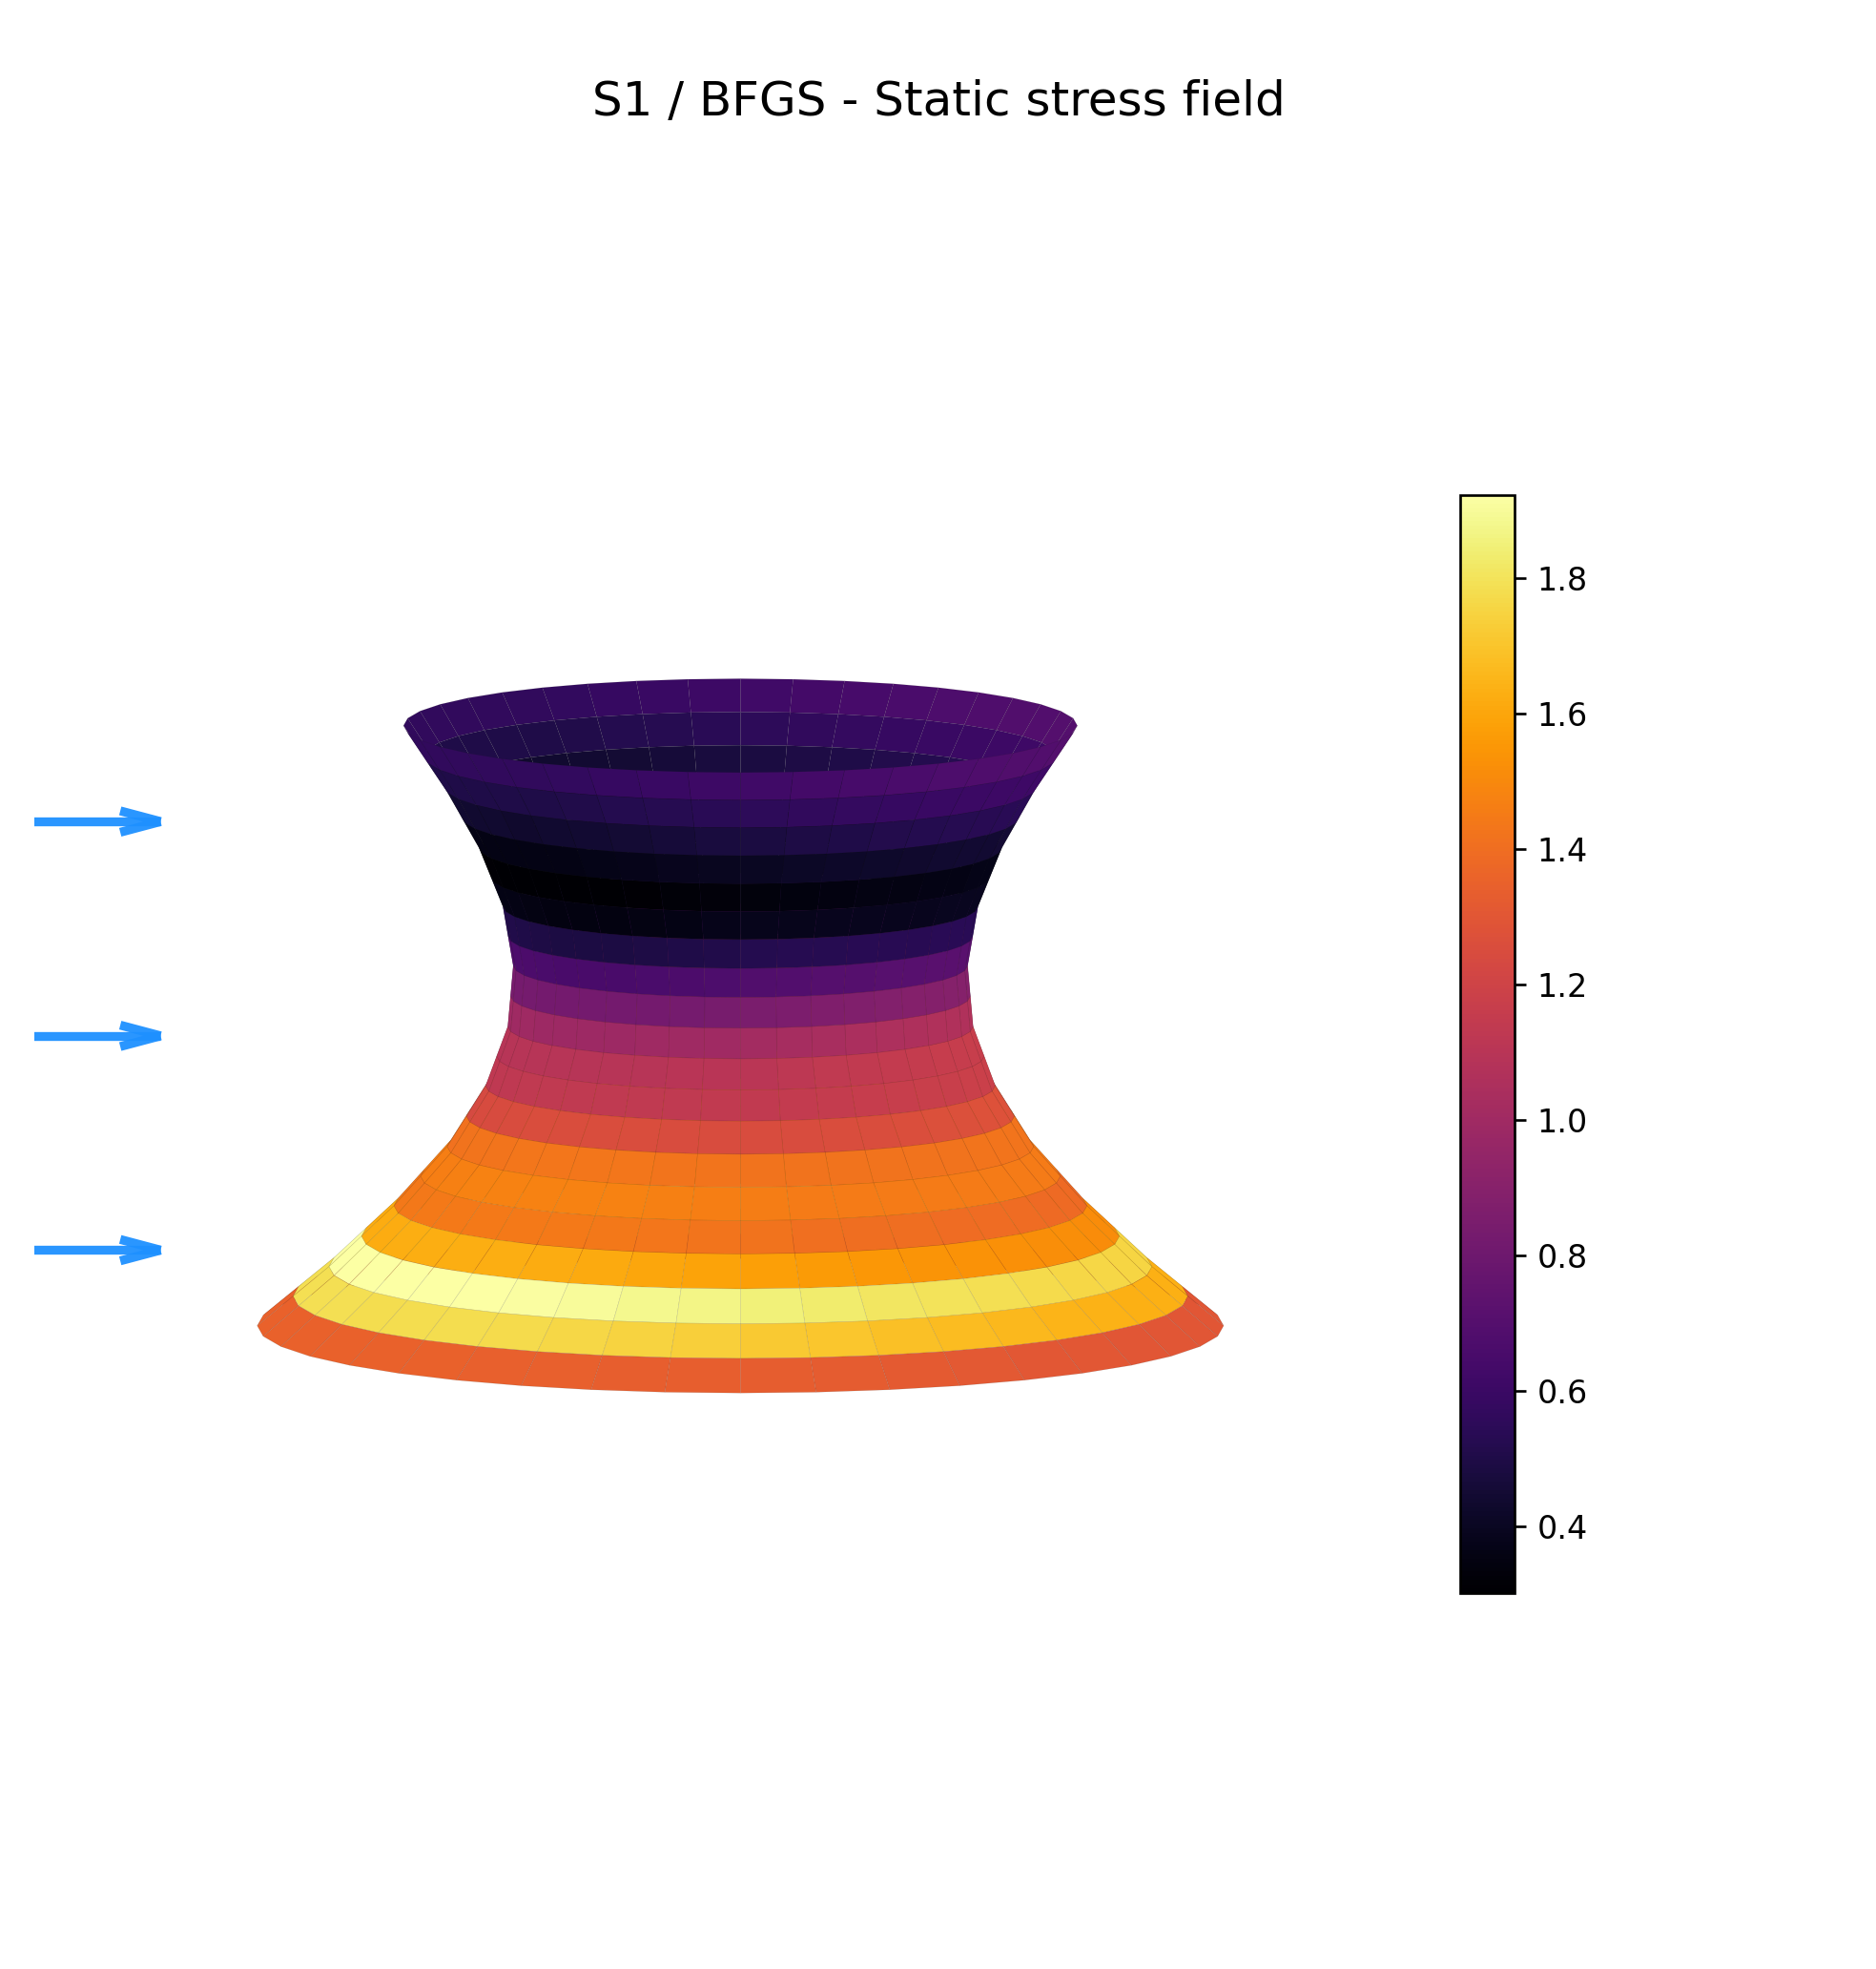
\includegraphics[width=\textwidth]{../results/figures/task7_s1_bfgs_stress.png}
\caption{S1 / BFGS stress}
\end{subfigure}\hfill
\begin{subfigure}{0.32\textwidth}
\centering
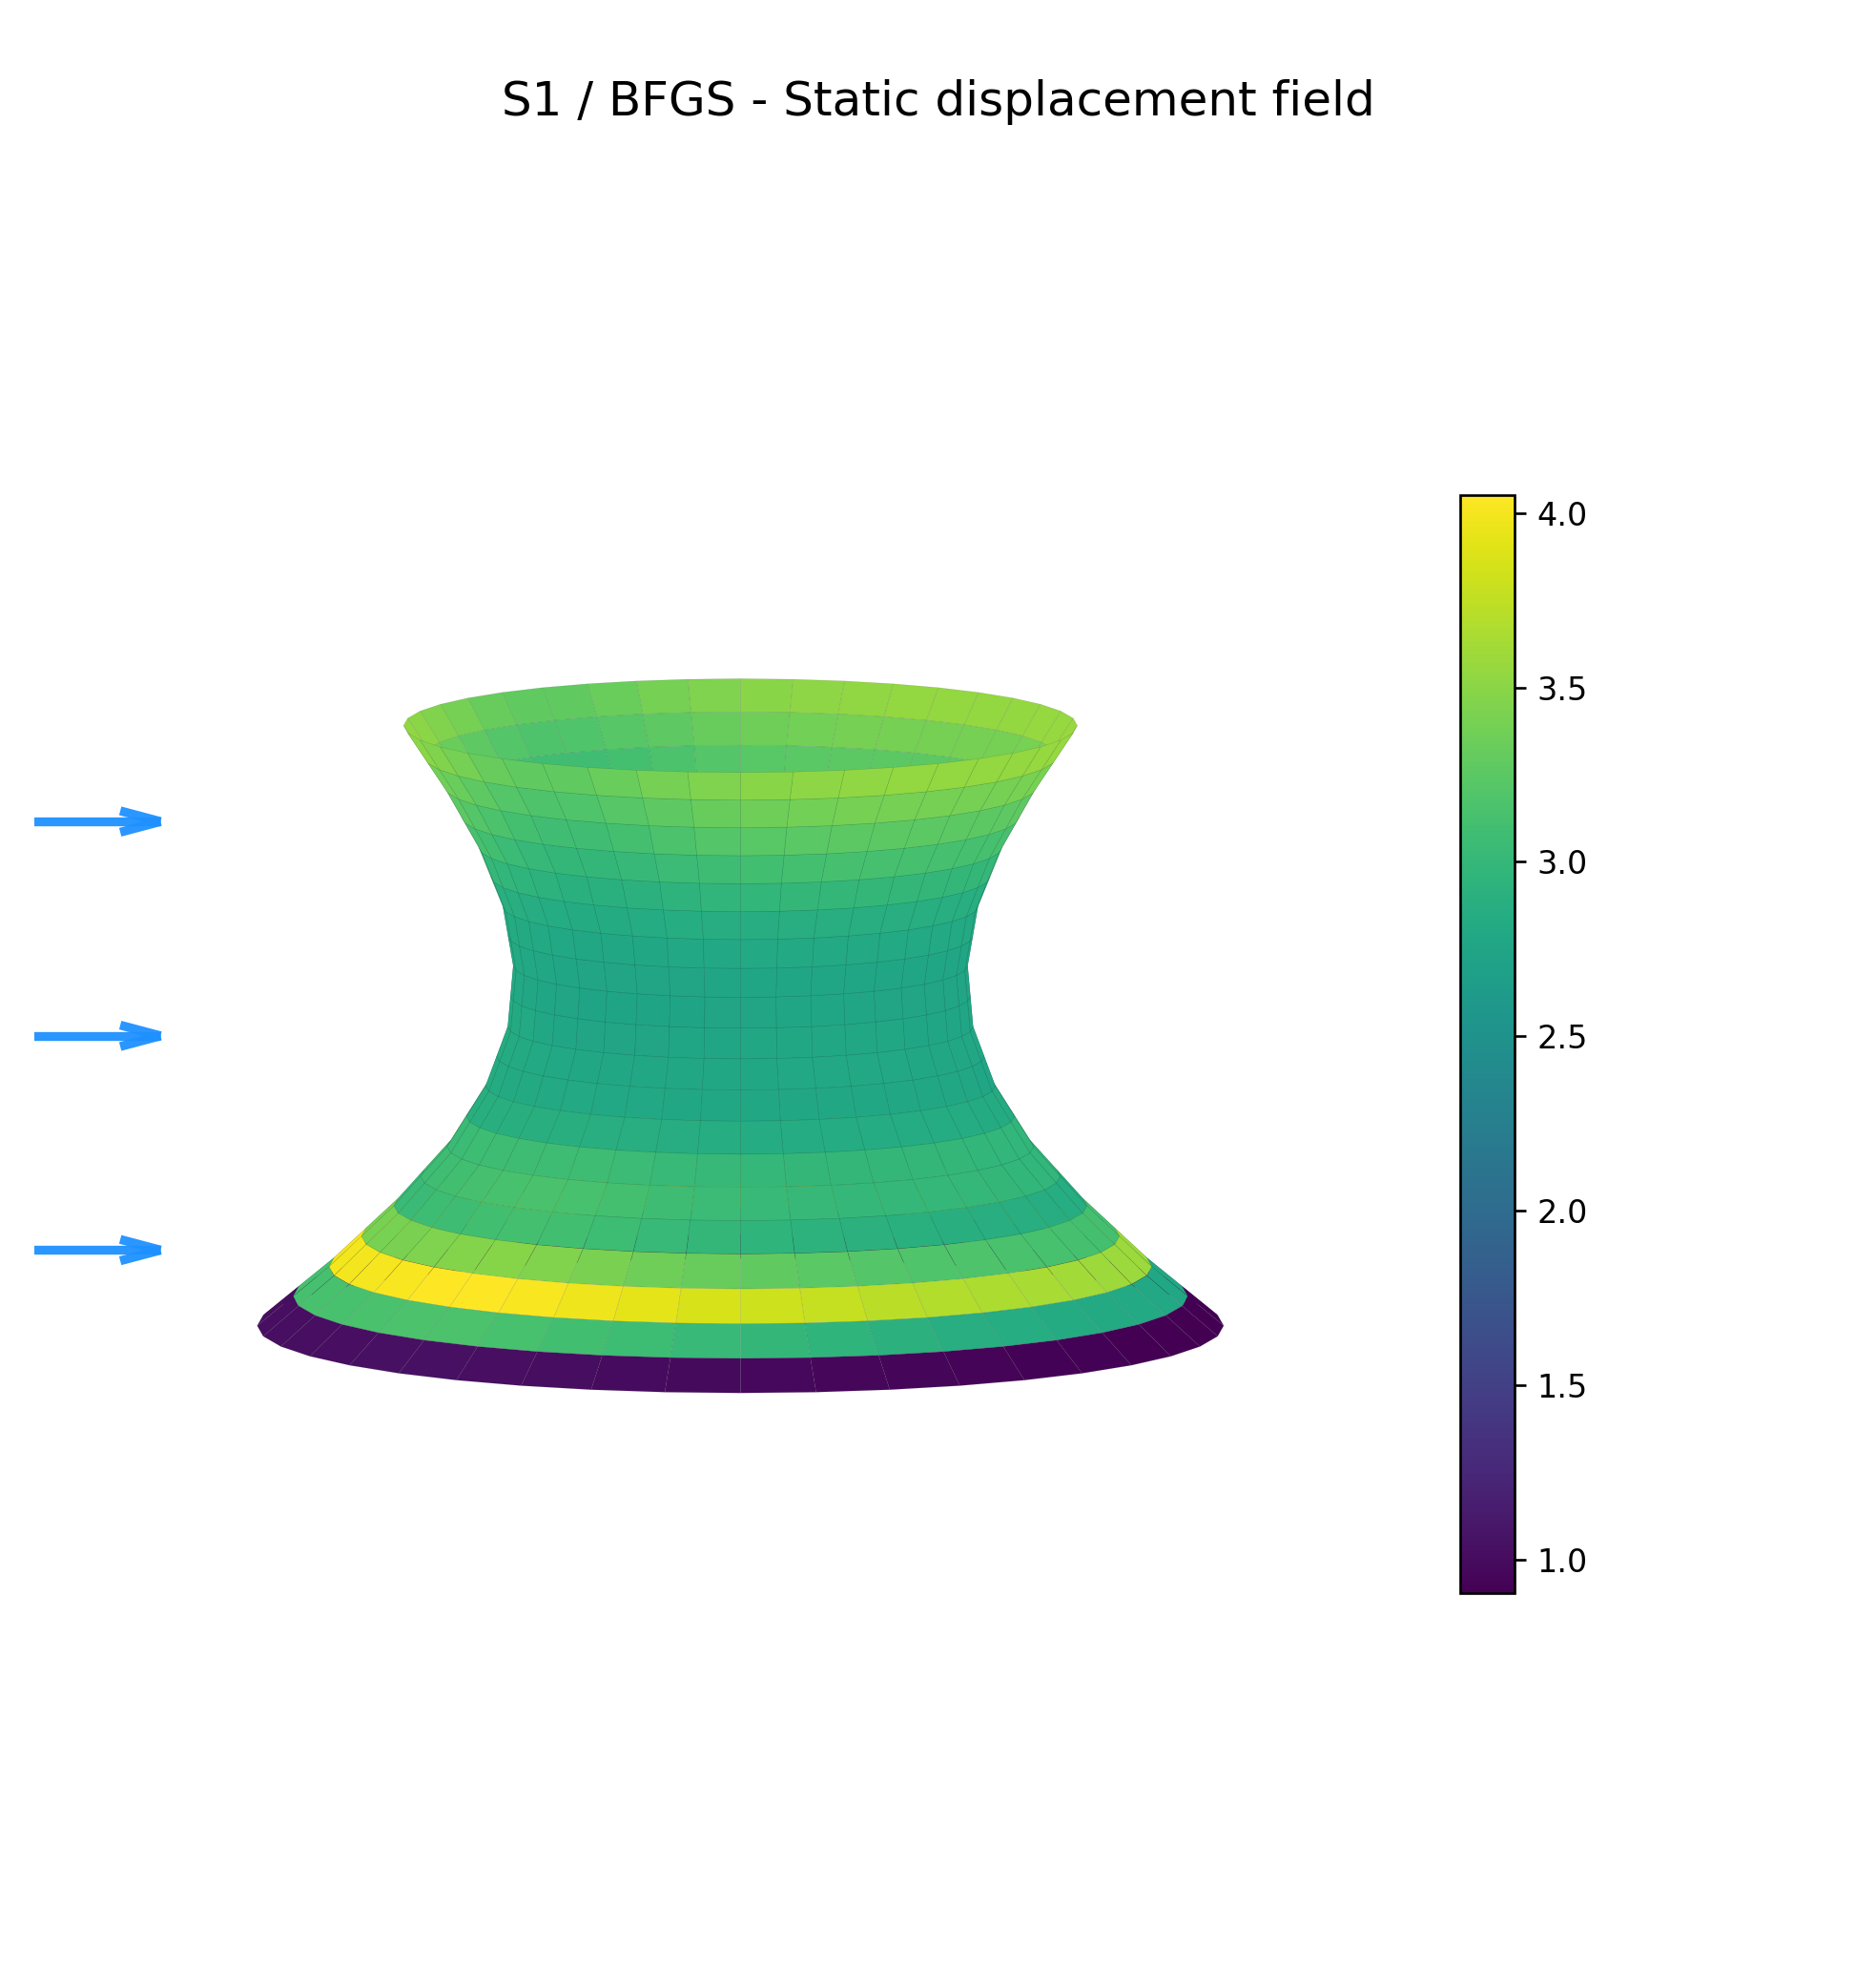
\includegraphics[width=\textwidth]{../results/figures/task7_s1_bfgs_displacement.png}
\caption{S1 / BFGS displacement}
\end{subfigure}\hfill
\begin{subfigure}{0.32\textwidth}
\centering
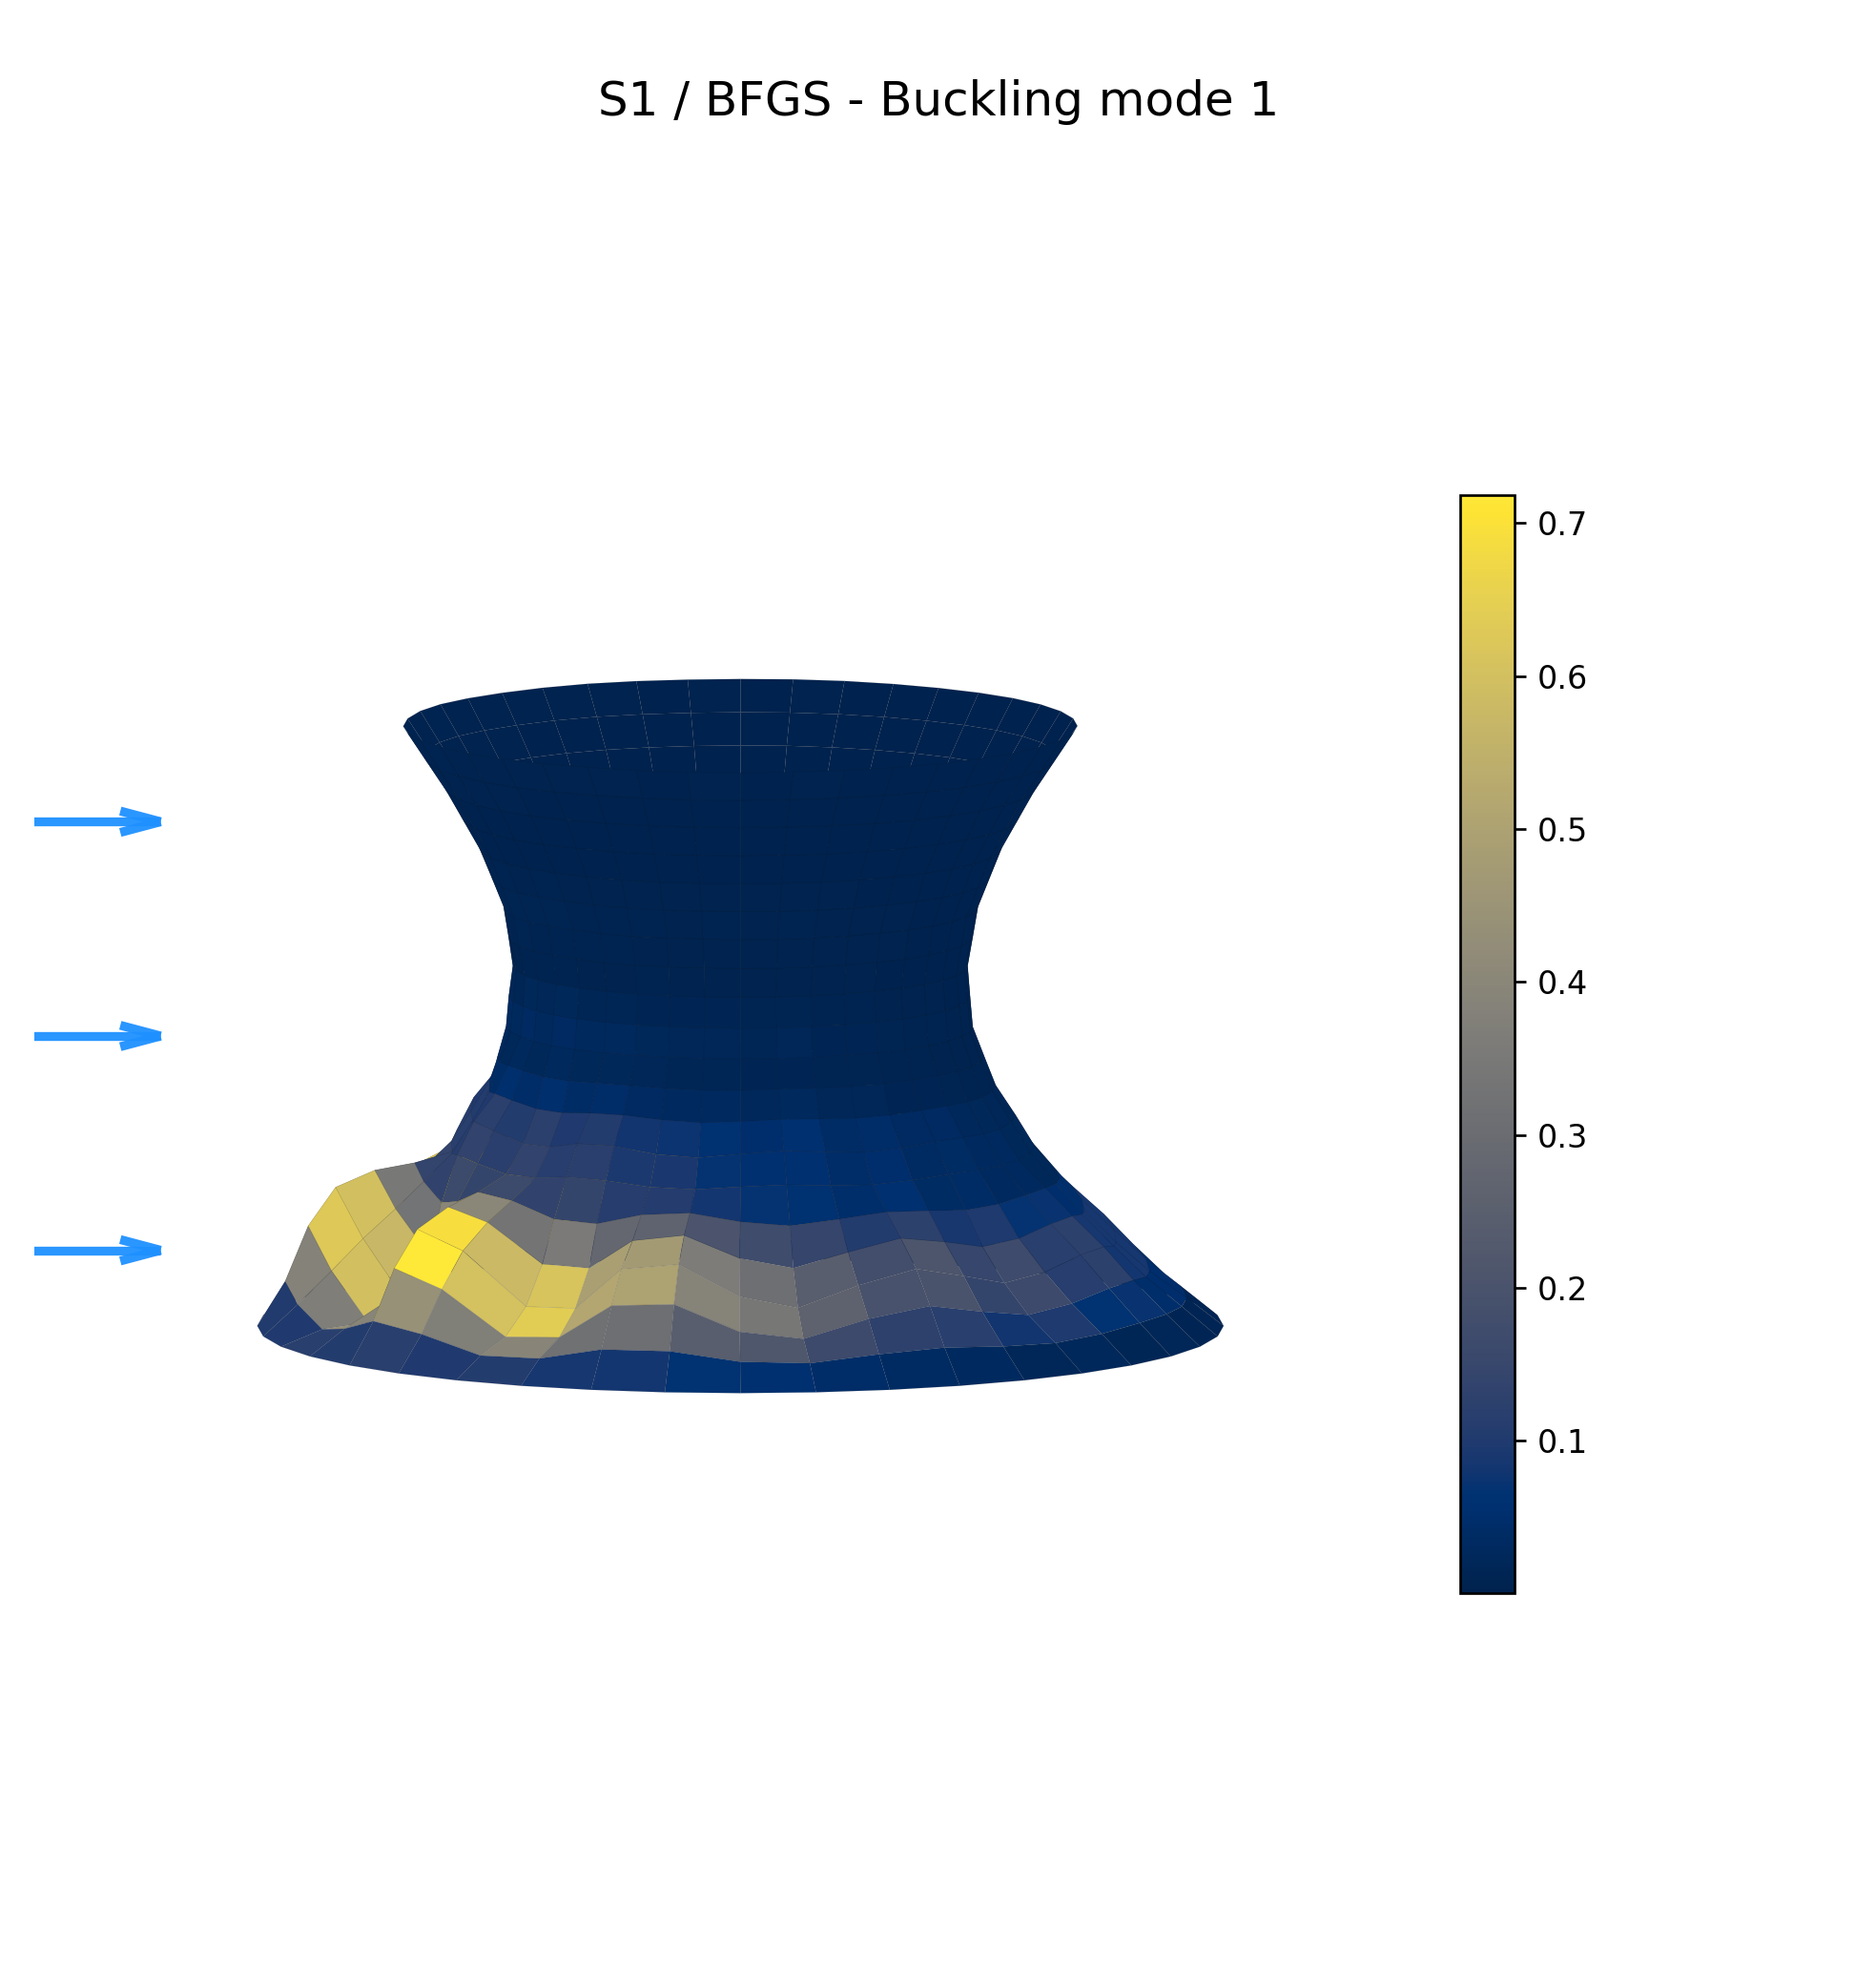
\includegraphics[width=\textwidth]{../results/figures/task7_s1_bfgs_buckling_mode1.png}
\caption{S1 / BFGS buckling}
\end{subfigure}
\caption{Combined visual fields}
\end{figure}


\subsection{S1 / PSO}


\begin{figure}[H]
\centering
\begin{subfigure}{0.32\textwidth}
\centering
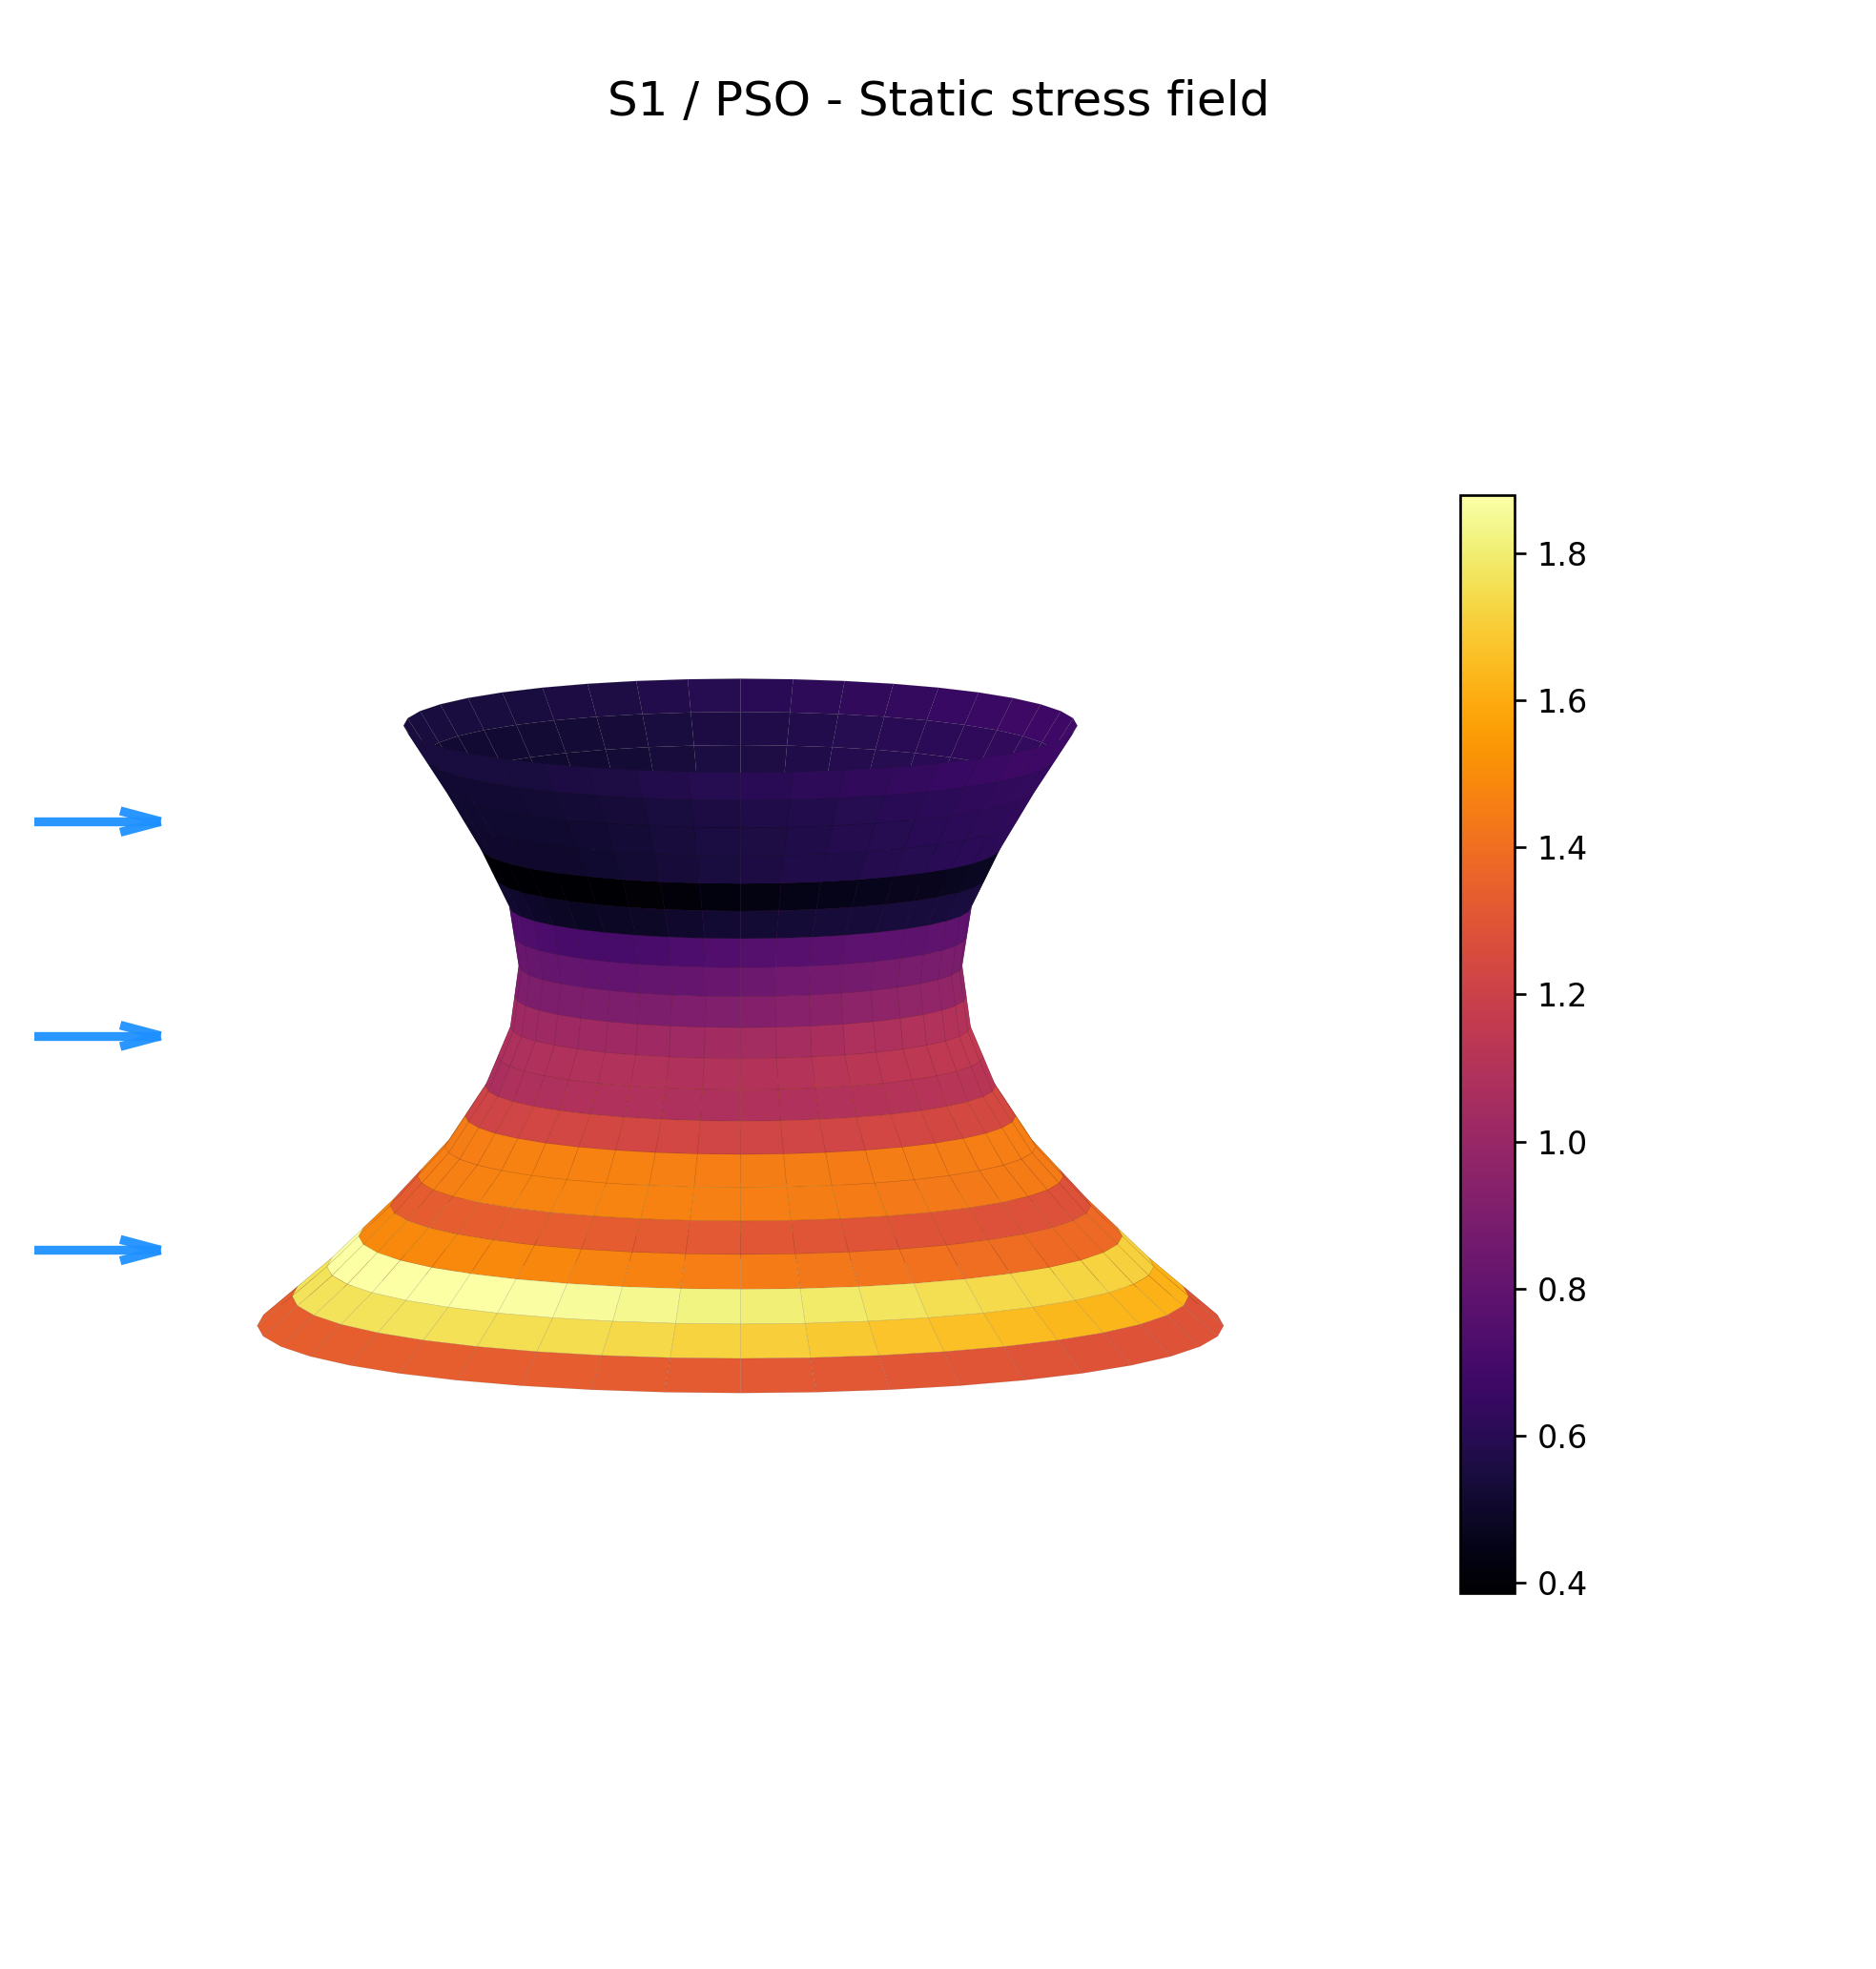
\includegraphics[width=\textwidth]{../results/figures/task7_s1_pso_stress.png}
\caption{S1 / PSO stress}
\end{subfigure}\hfill
\begin{subfigure}{0.32\textwidth}
\centering
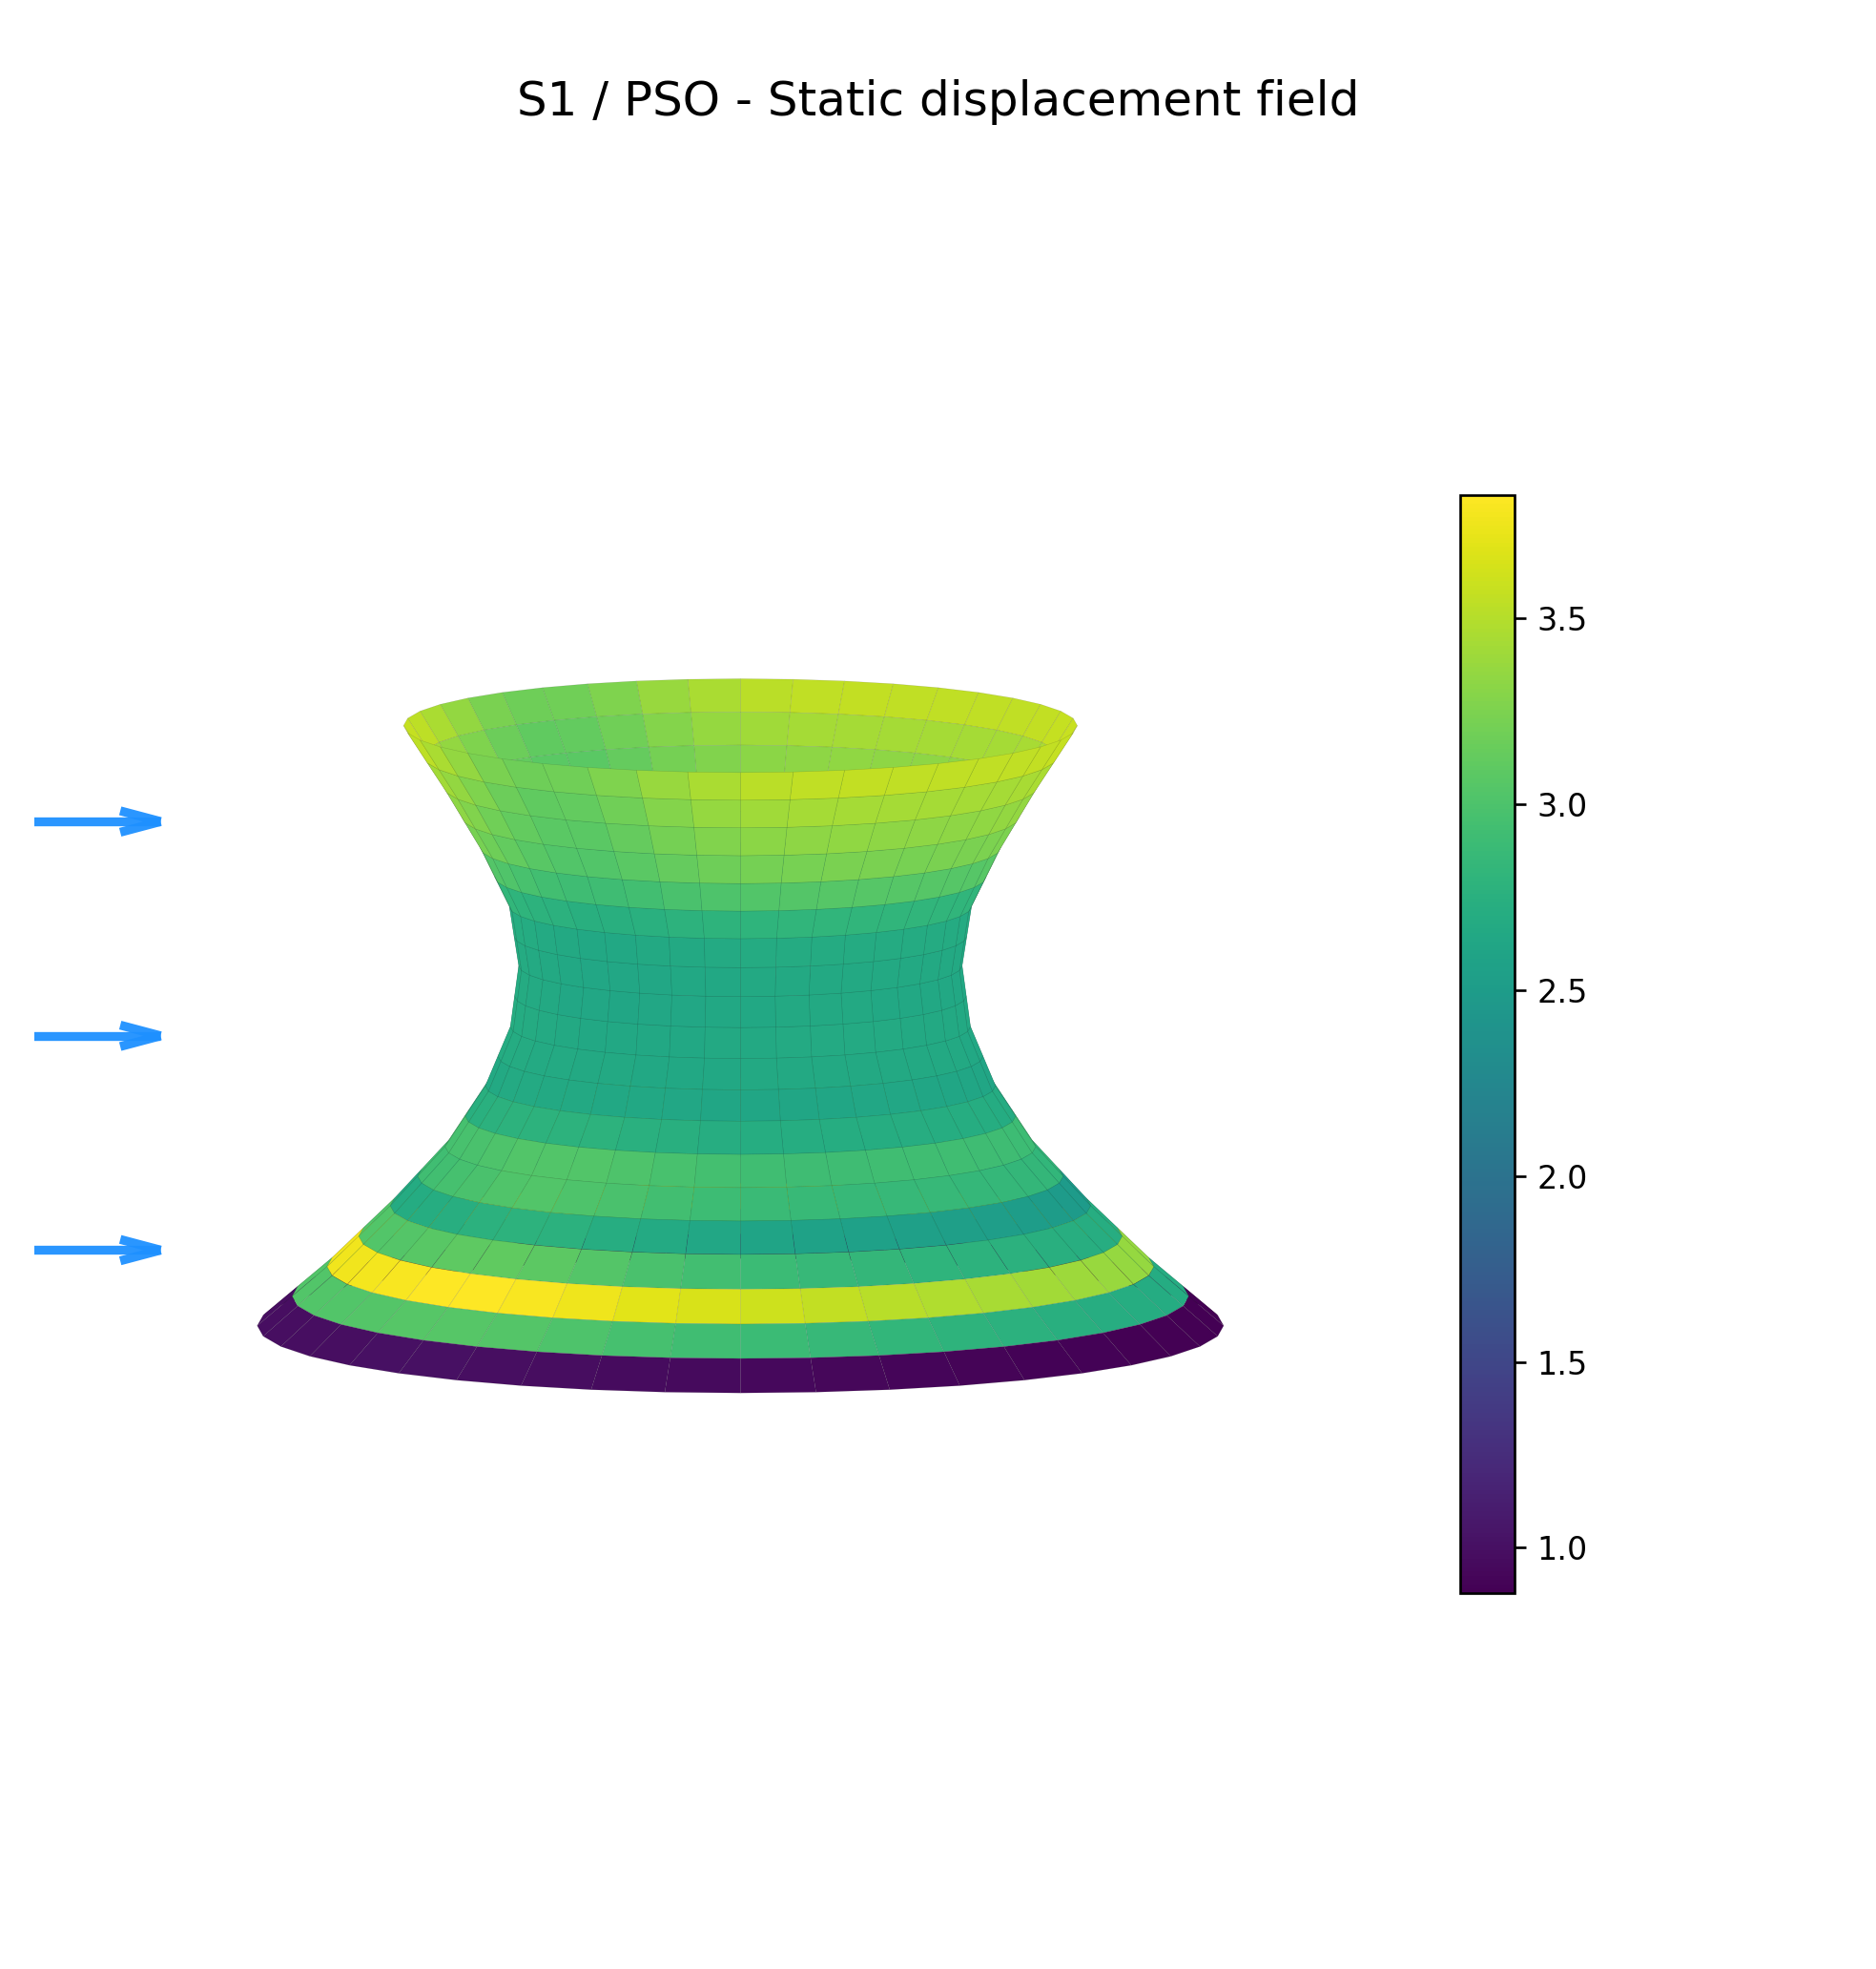
\includegraphics[width=\textwidth]{../results/figures/task7_s1_pso_displacement.png}
\caption{S1 / PSO displacement}
\end{subfigure}\hfill
\begin{subfigure}{0.32\textwidth}
\centering
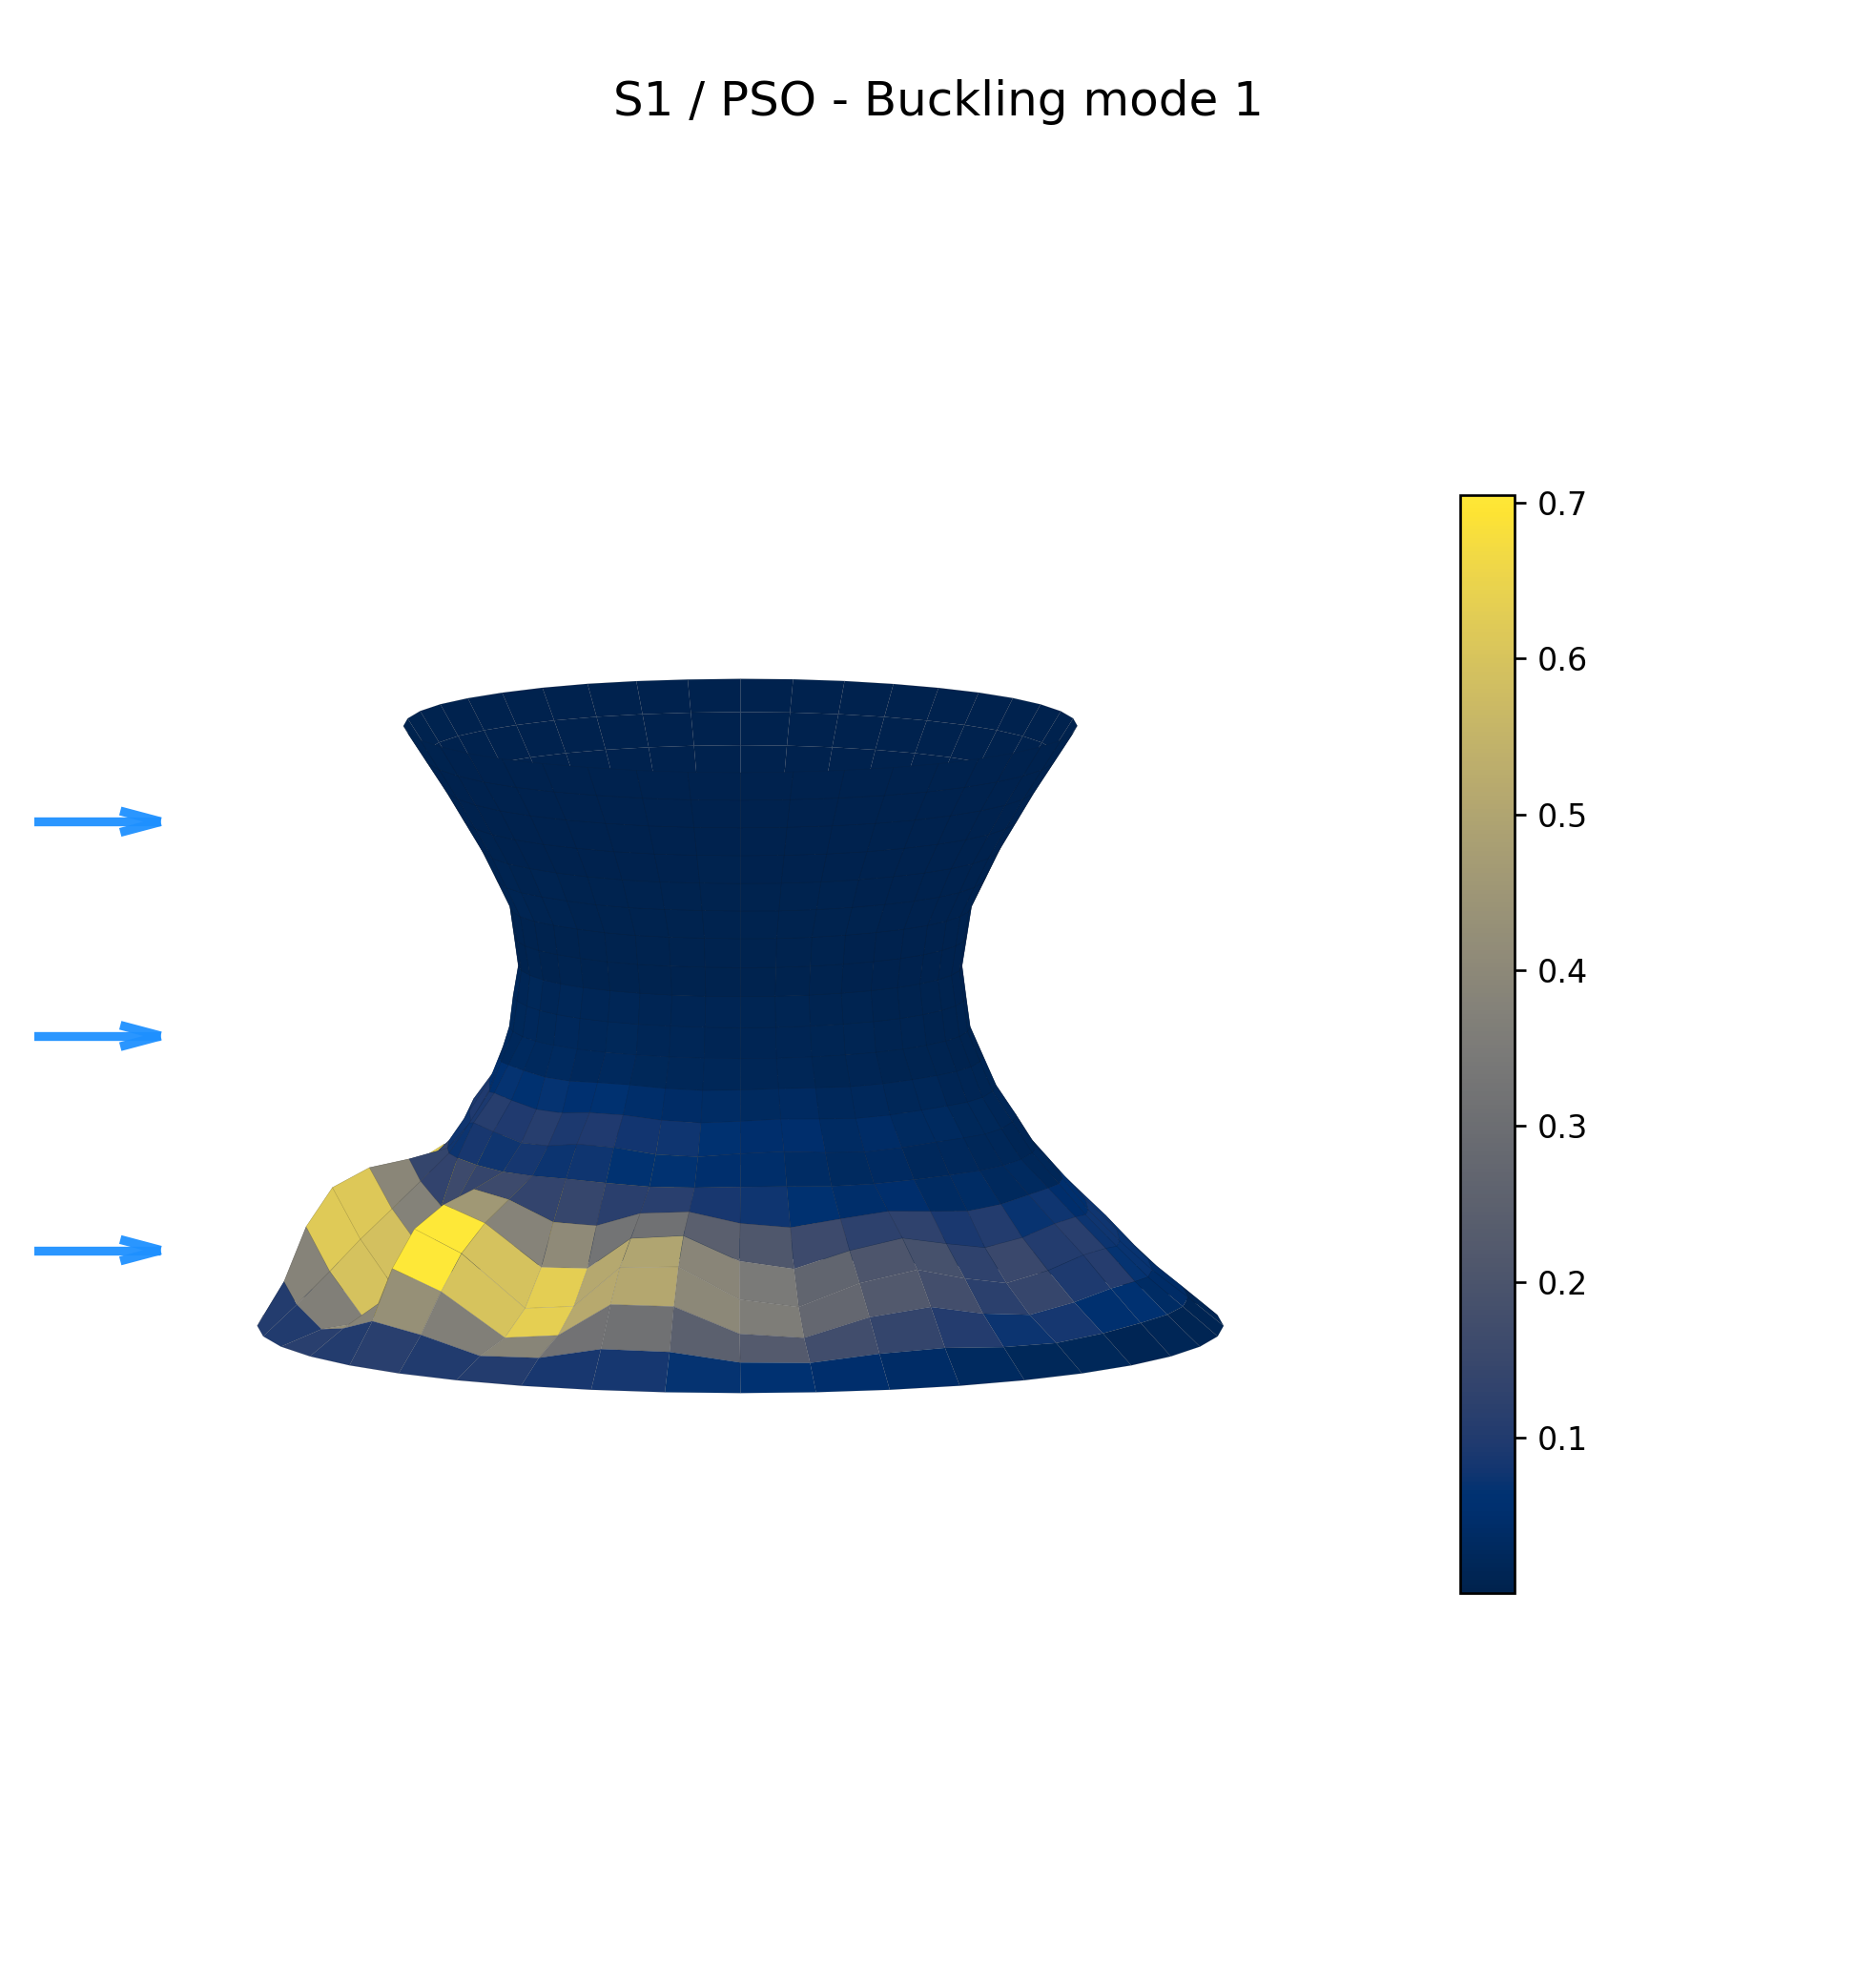
\includegraphics[width=\textwidth]{../results/figures/task7_s1_pso_buckling_mode1.png}
\caption{S1 / PSO buckling}
\end{subfigure}
\caption{Combined visual fields}
\end{figure}


\subsection{S1 / SA}


\begin{figure}[H]
\centering
\begin{subfigure}{0.32\textwidth}
\centering
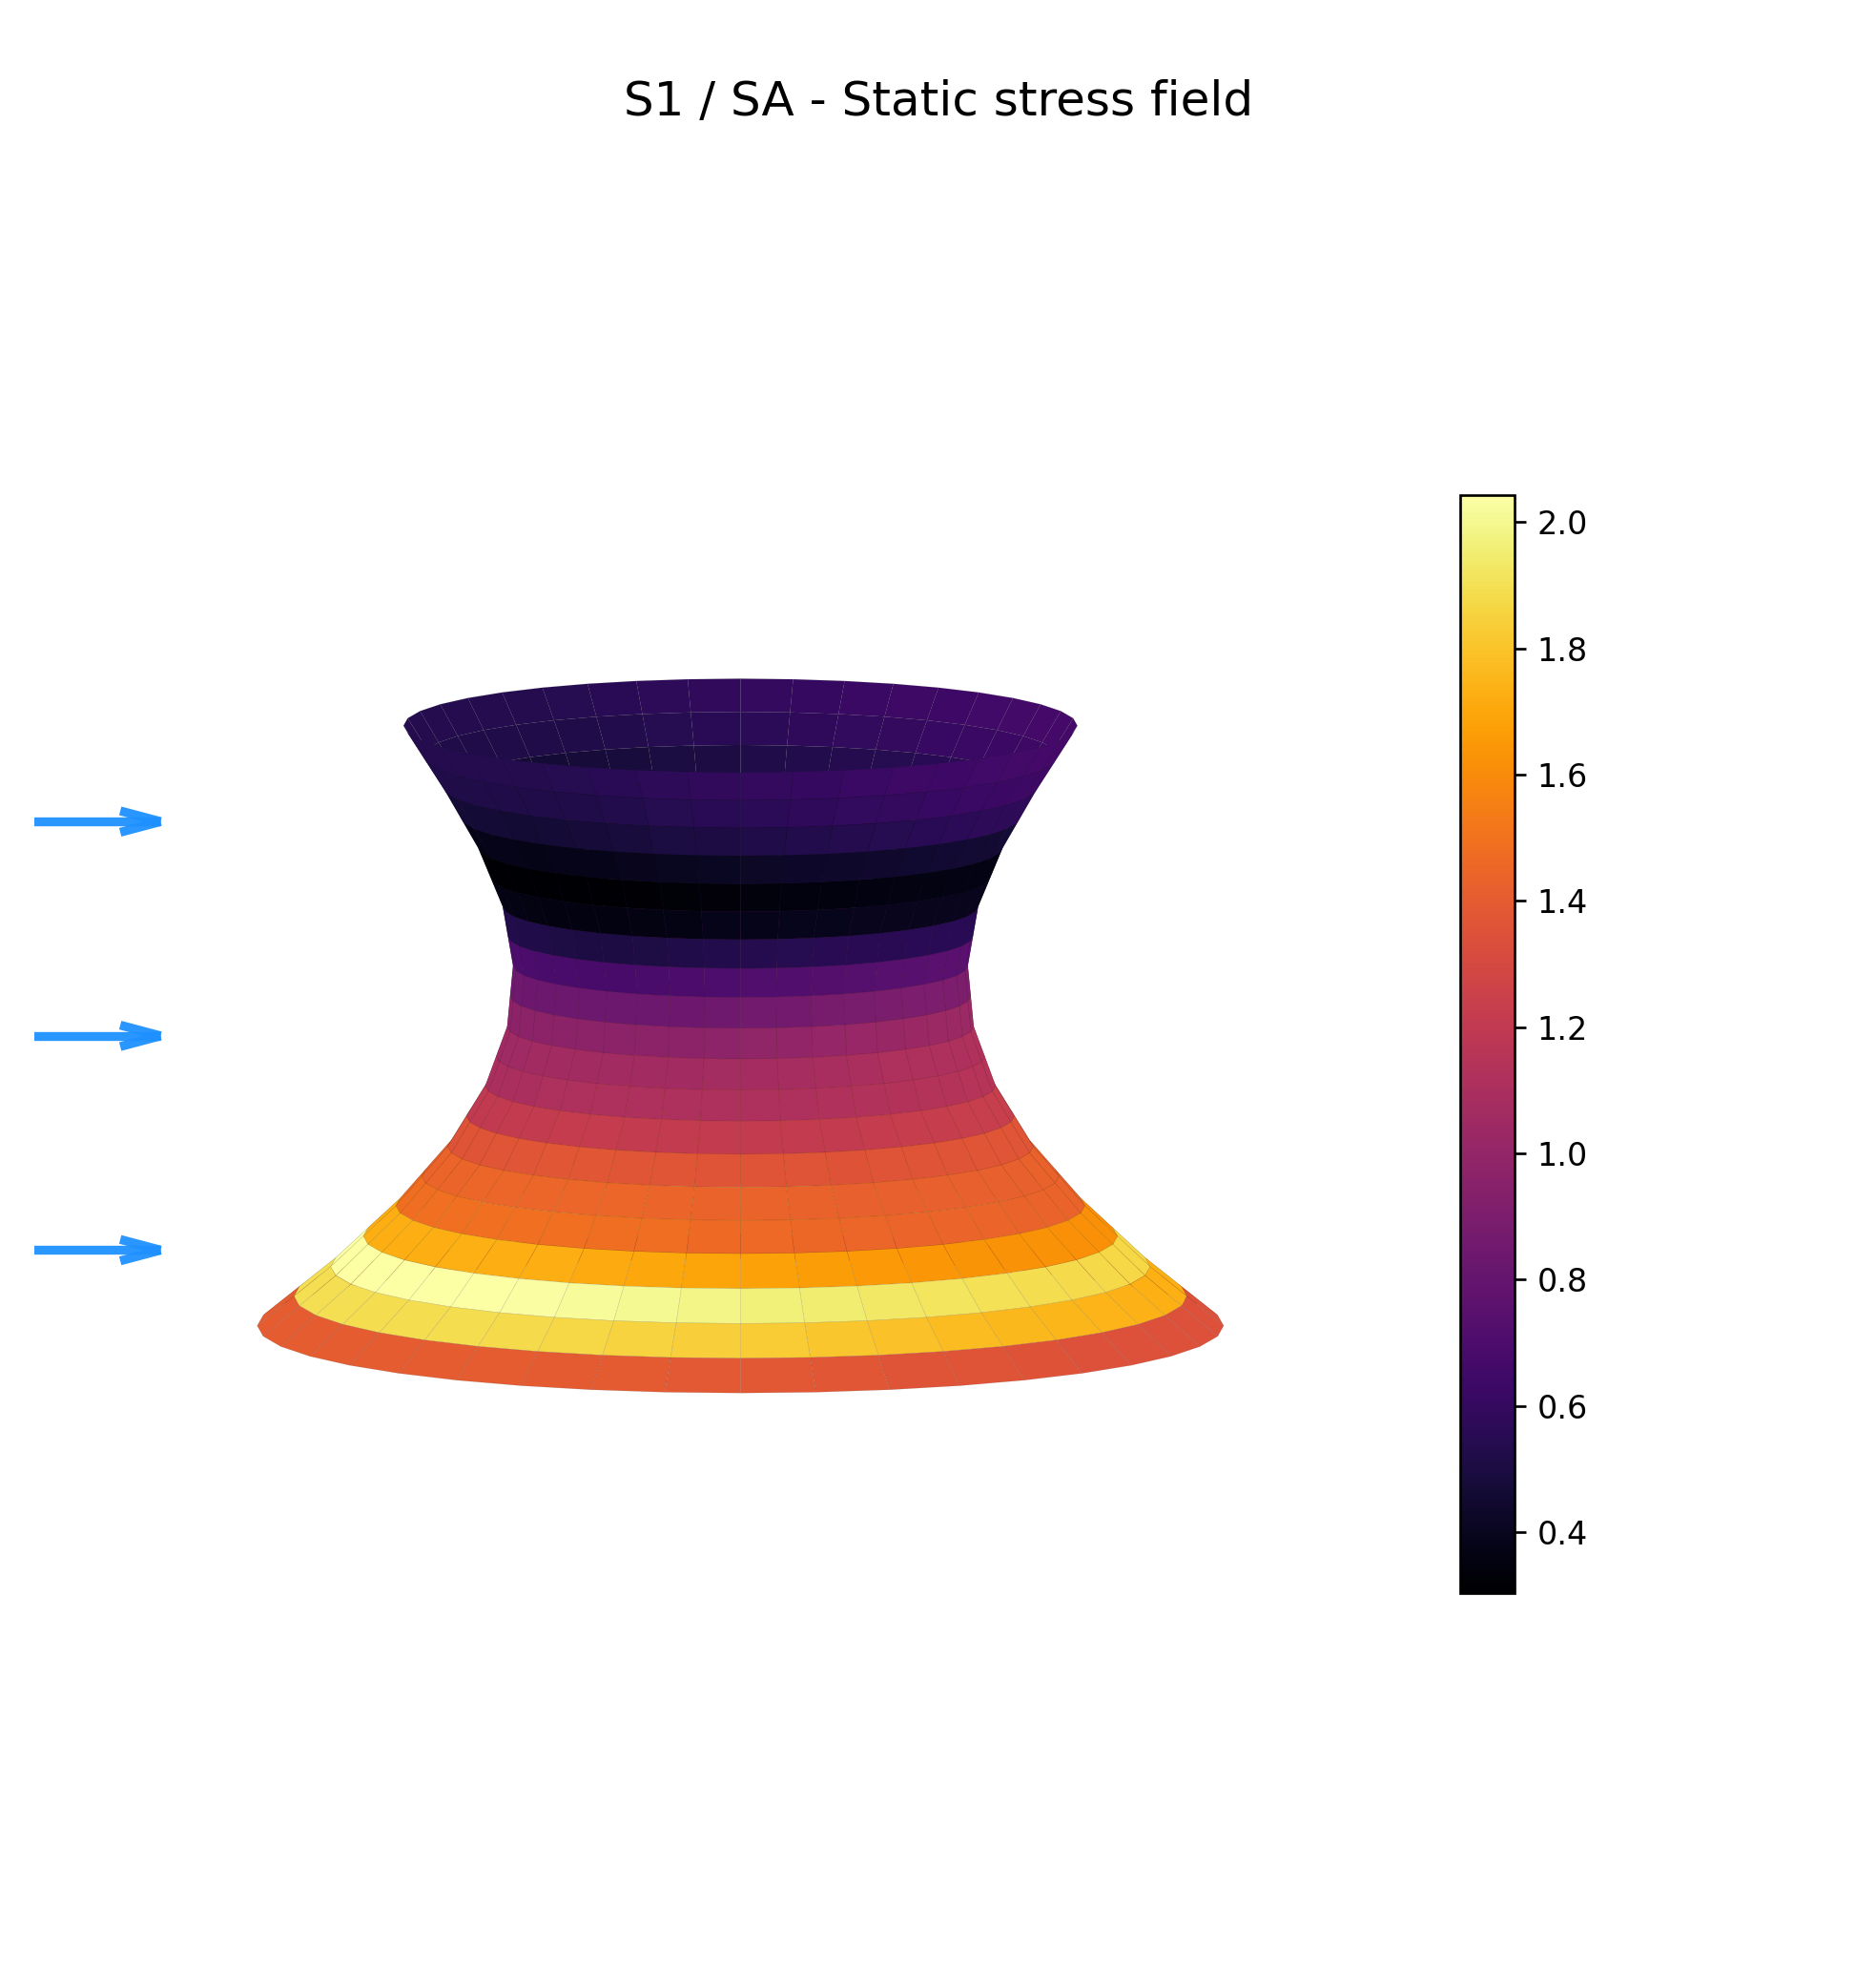
\includegraphics[width=\textwidth]{../results/figures/task7_s1_sa_stress.png}
\caption{S1 / SA stress}
\end{subfigure}\hfill
\begin{subfigure}{0.32\textwidth}
\centering
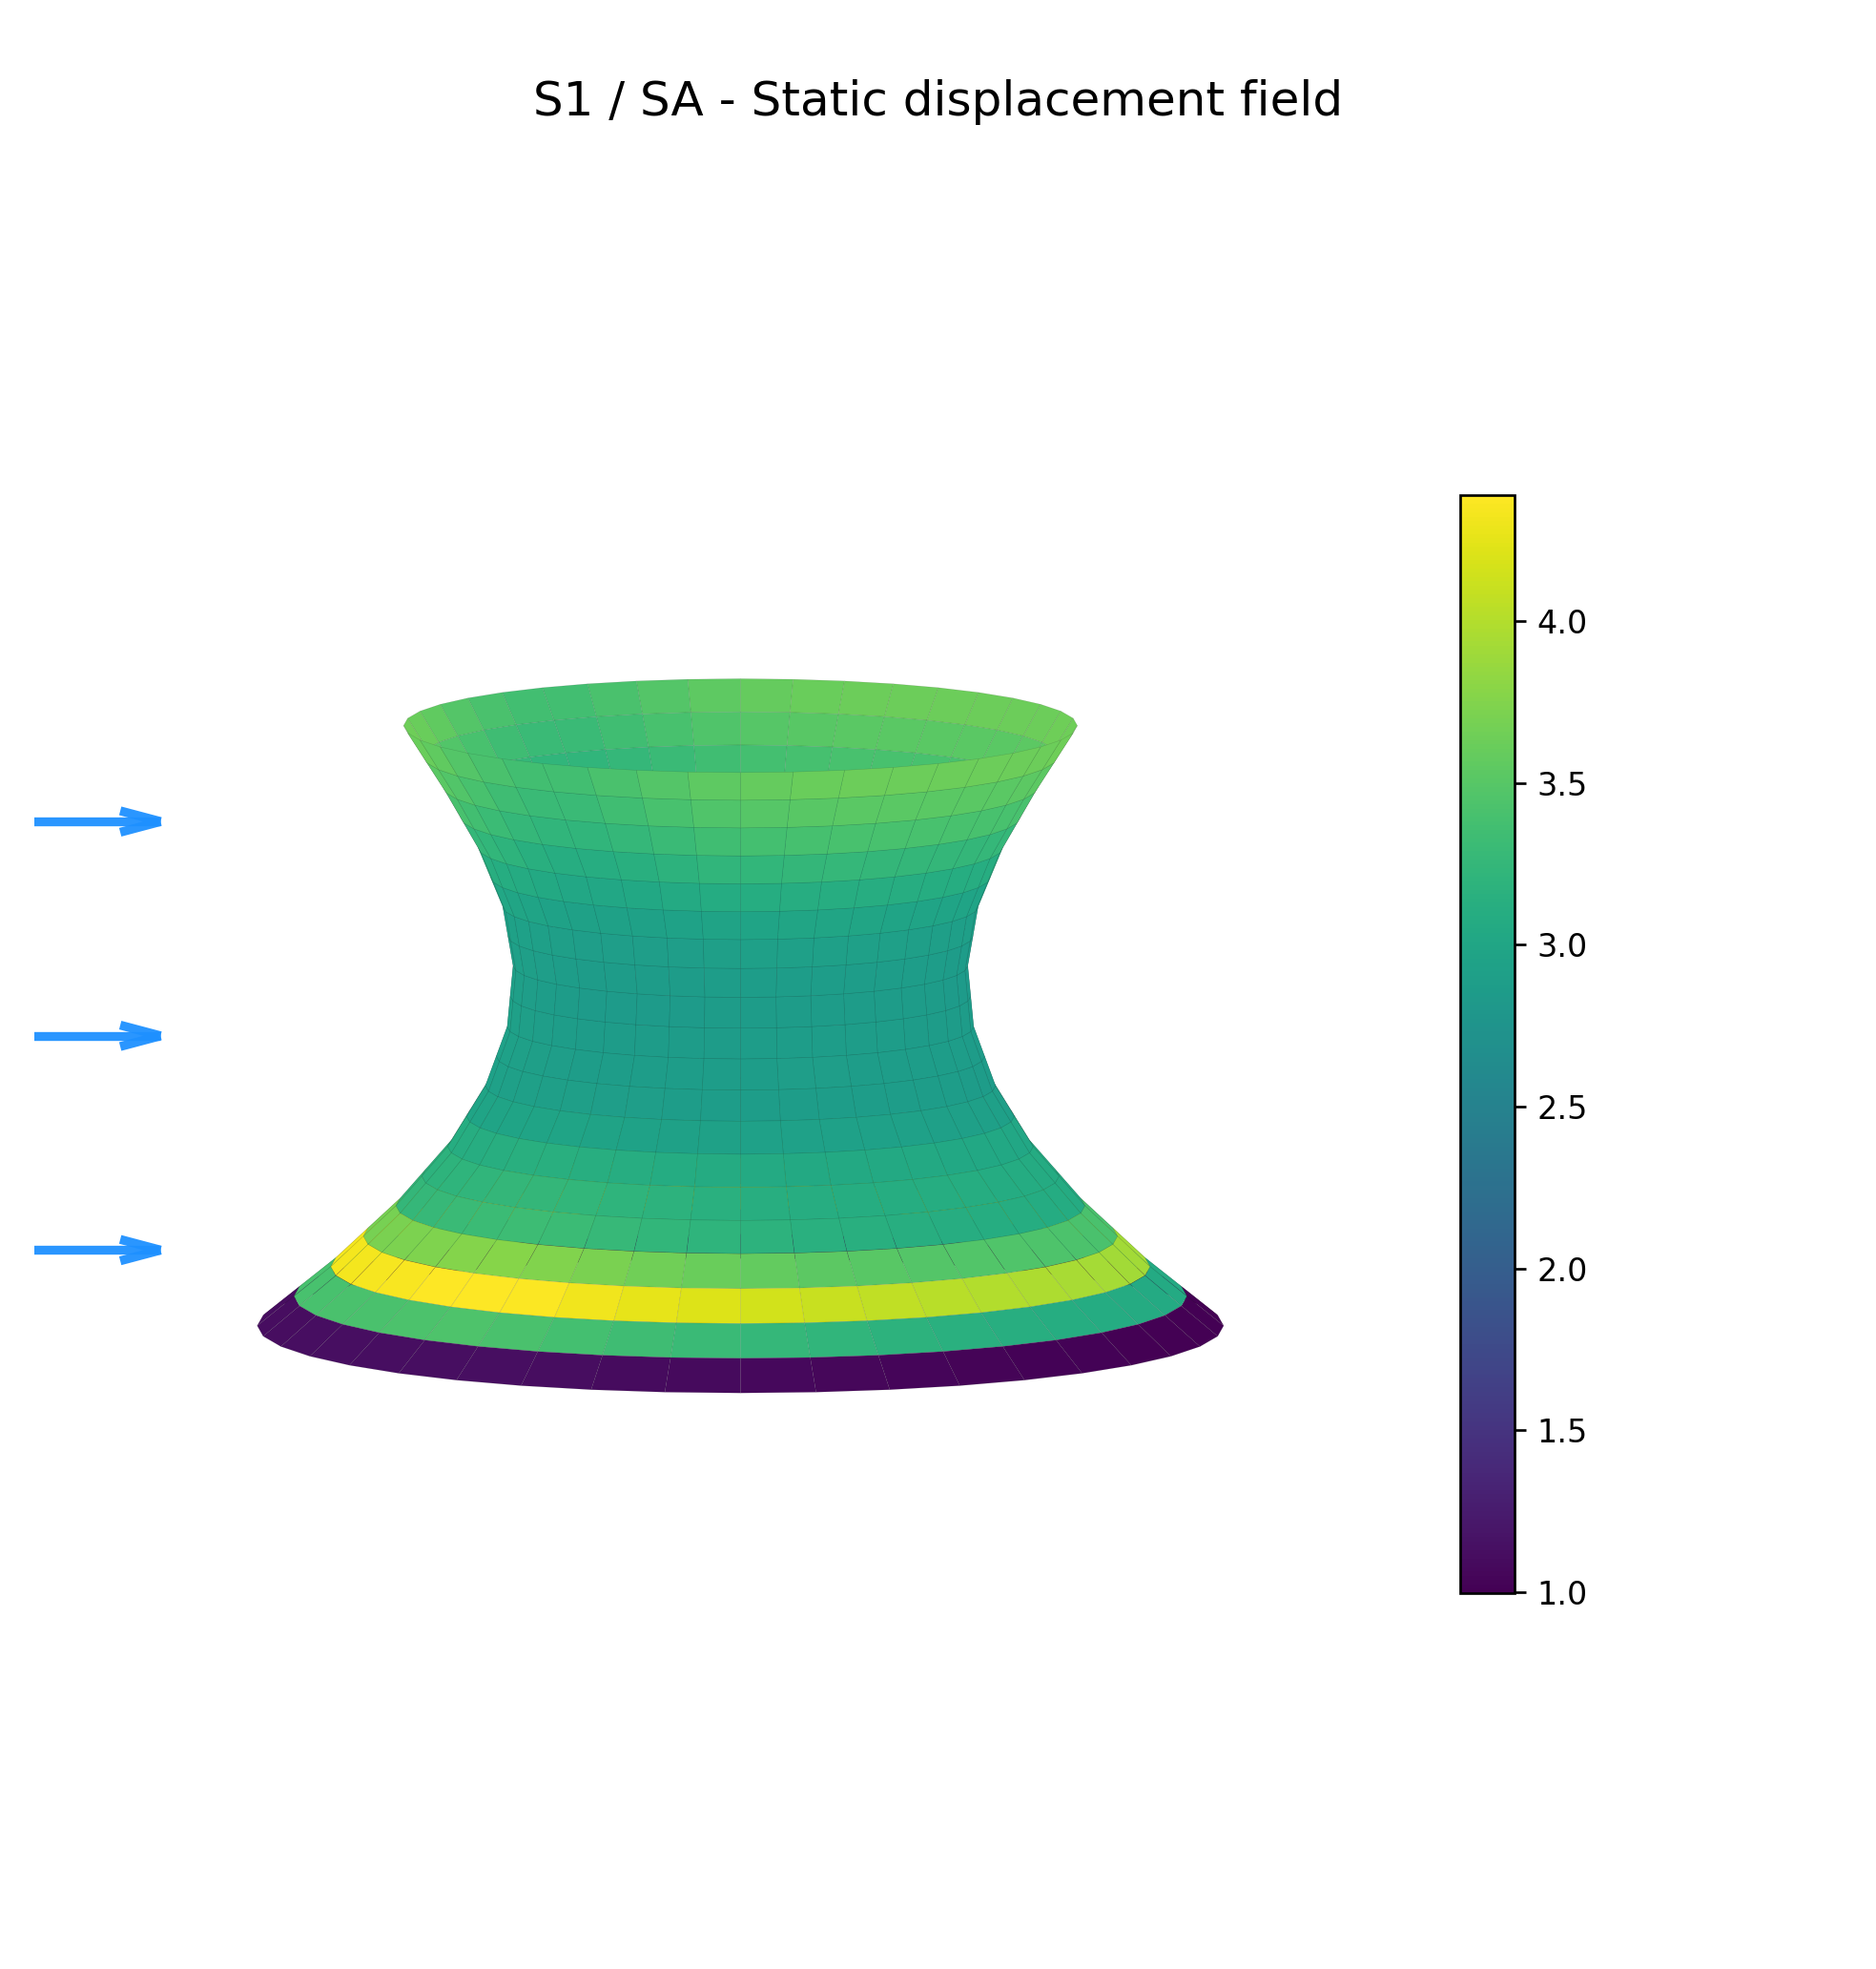
\includegraphics[width=\textwidth]{../results/figures/task7_s1_sa_displacement.png}
\caption{S1 / SA displacement}
\end{subfigure}\hfill
\begin{subfigure}{0.32\textwidth}
\centering
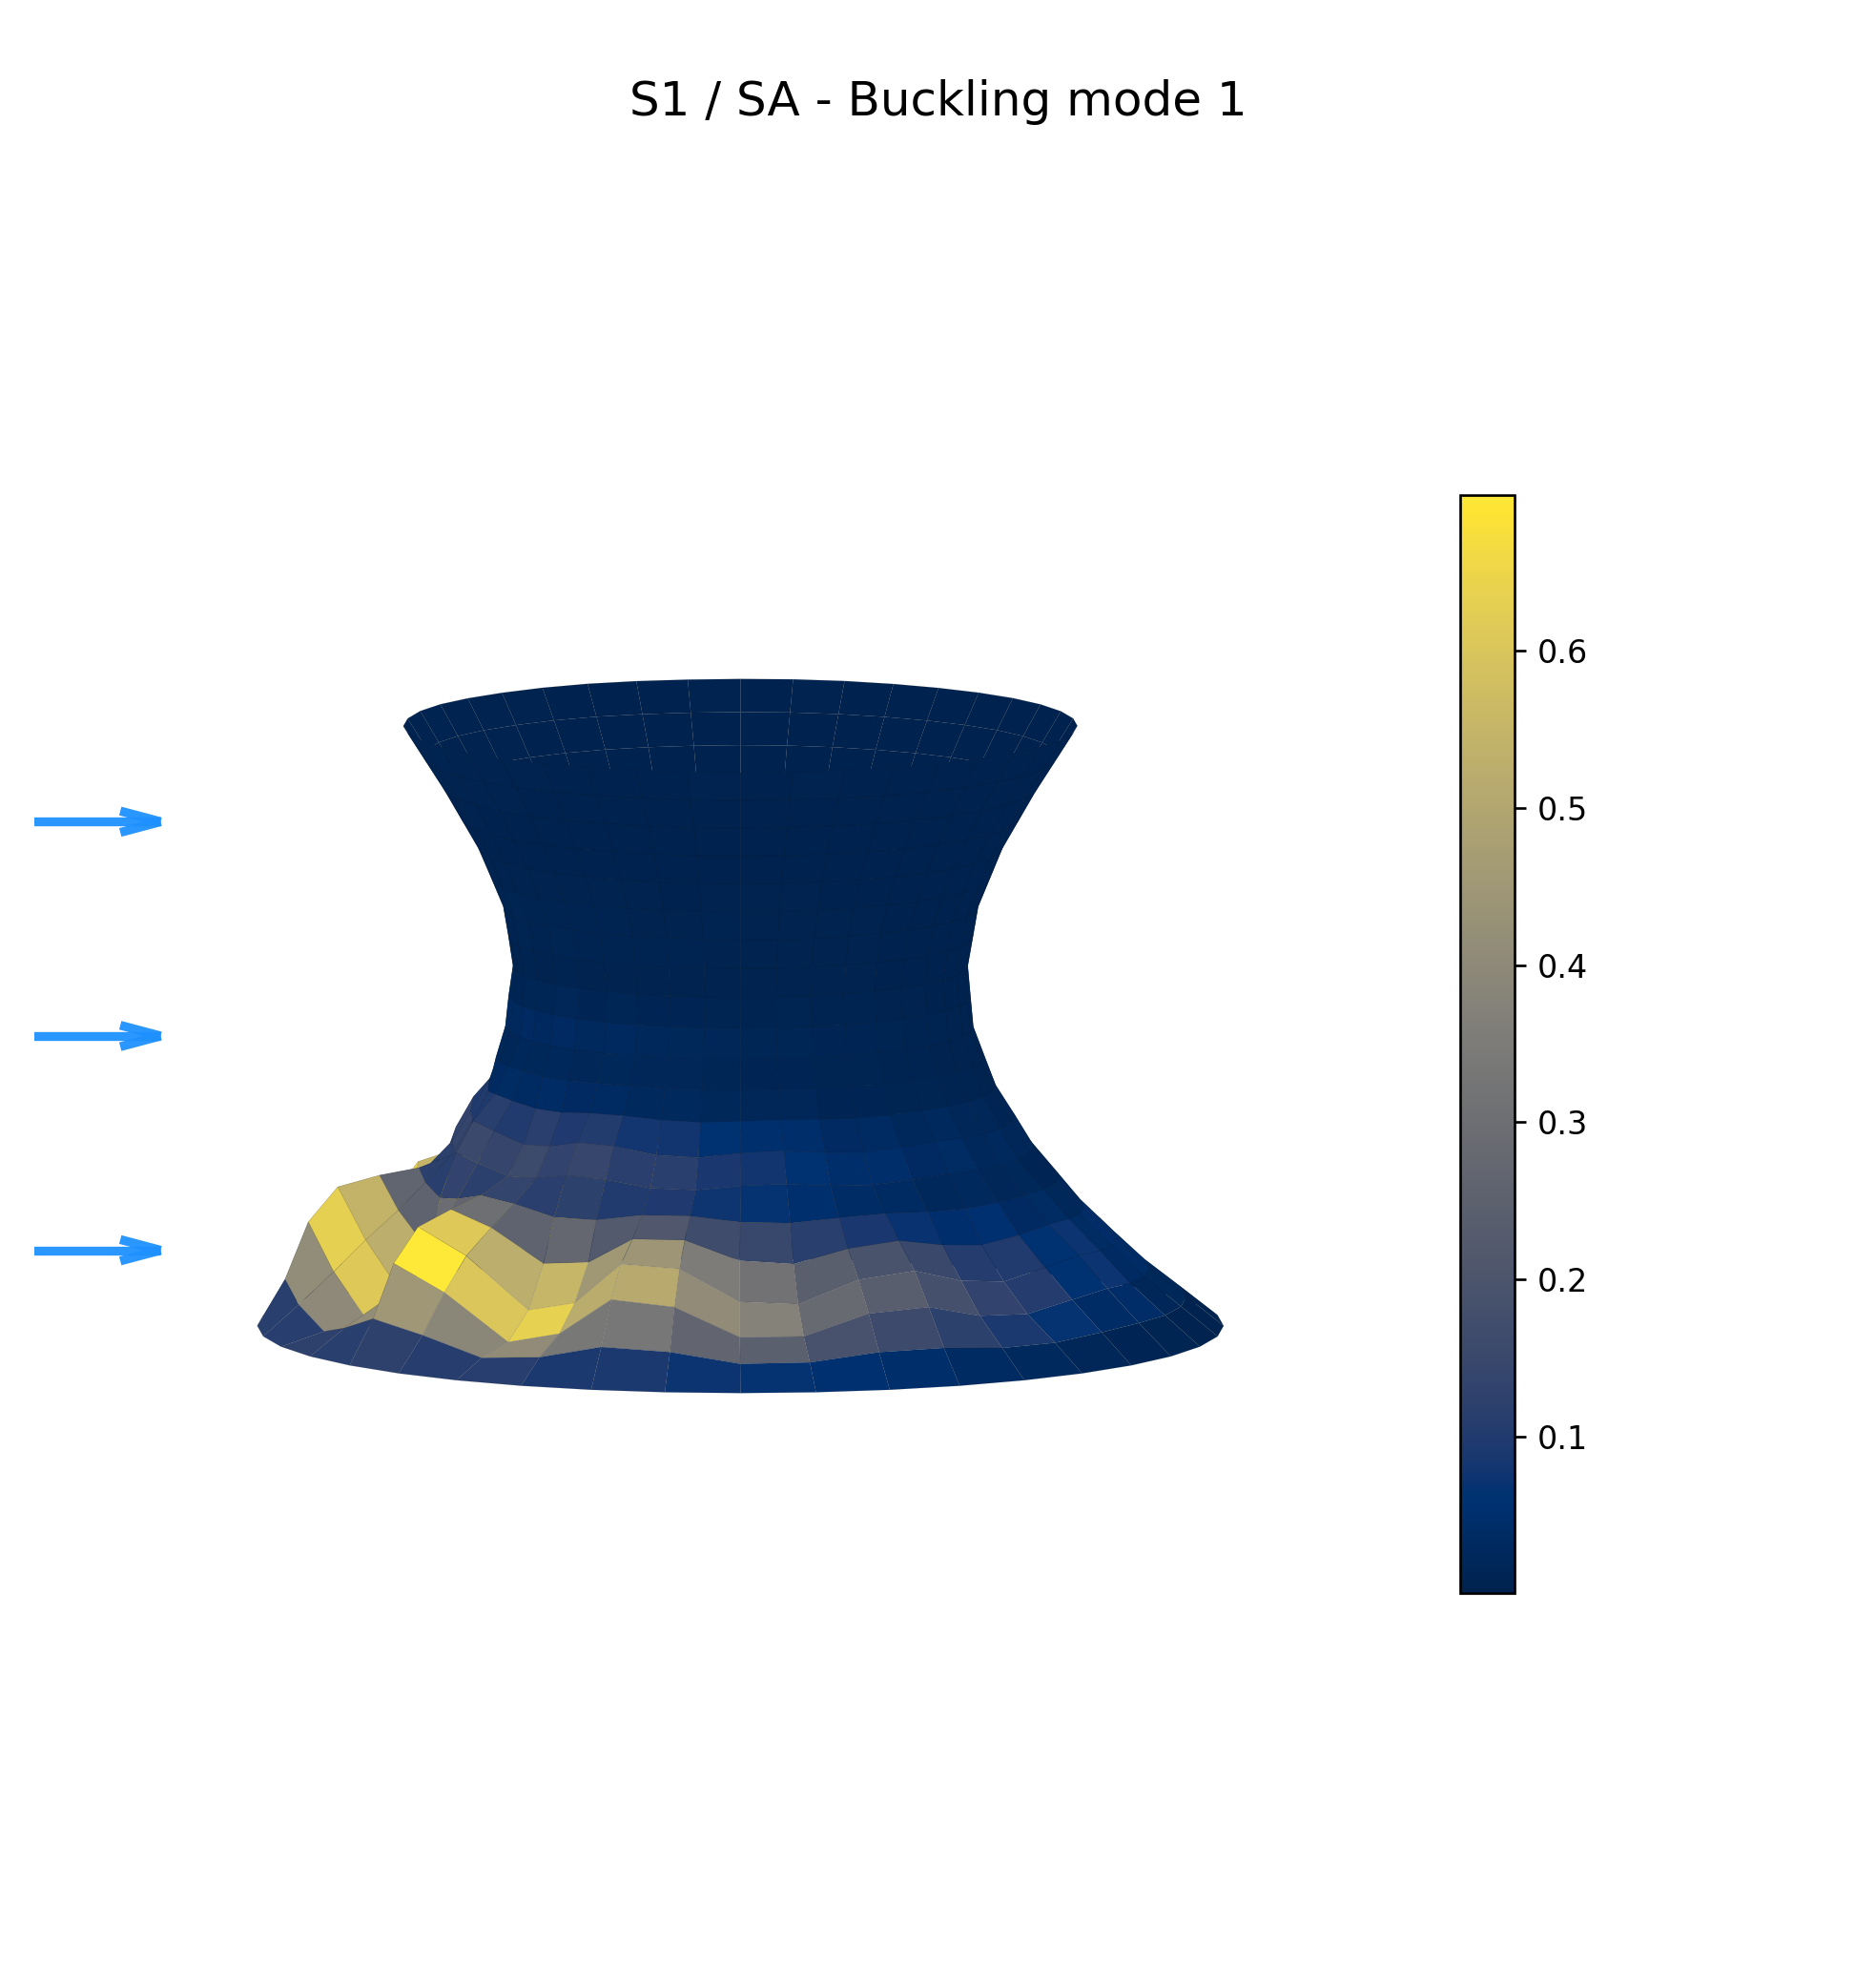
\includegraphics[width=\textwidth]{../results/figures/task7_s1_sa_buckling_mode1.png}
\caption{S1 / SA buckling}
\end{subfigure}
\caption{Combined visual fields}
\end{figure}


\section{Scenario S2}


\subsection{S2 / PSO}


\begin{figure}[H]
\centering
\begin{subfigure}{0.32\textwidth}
\centering
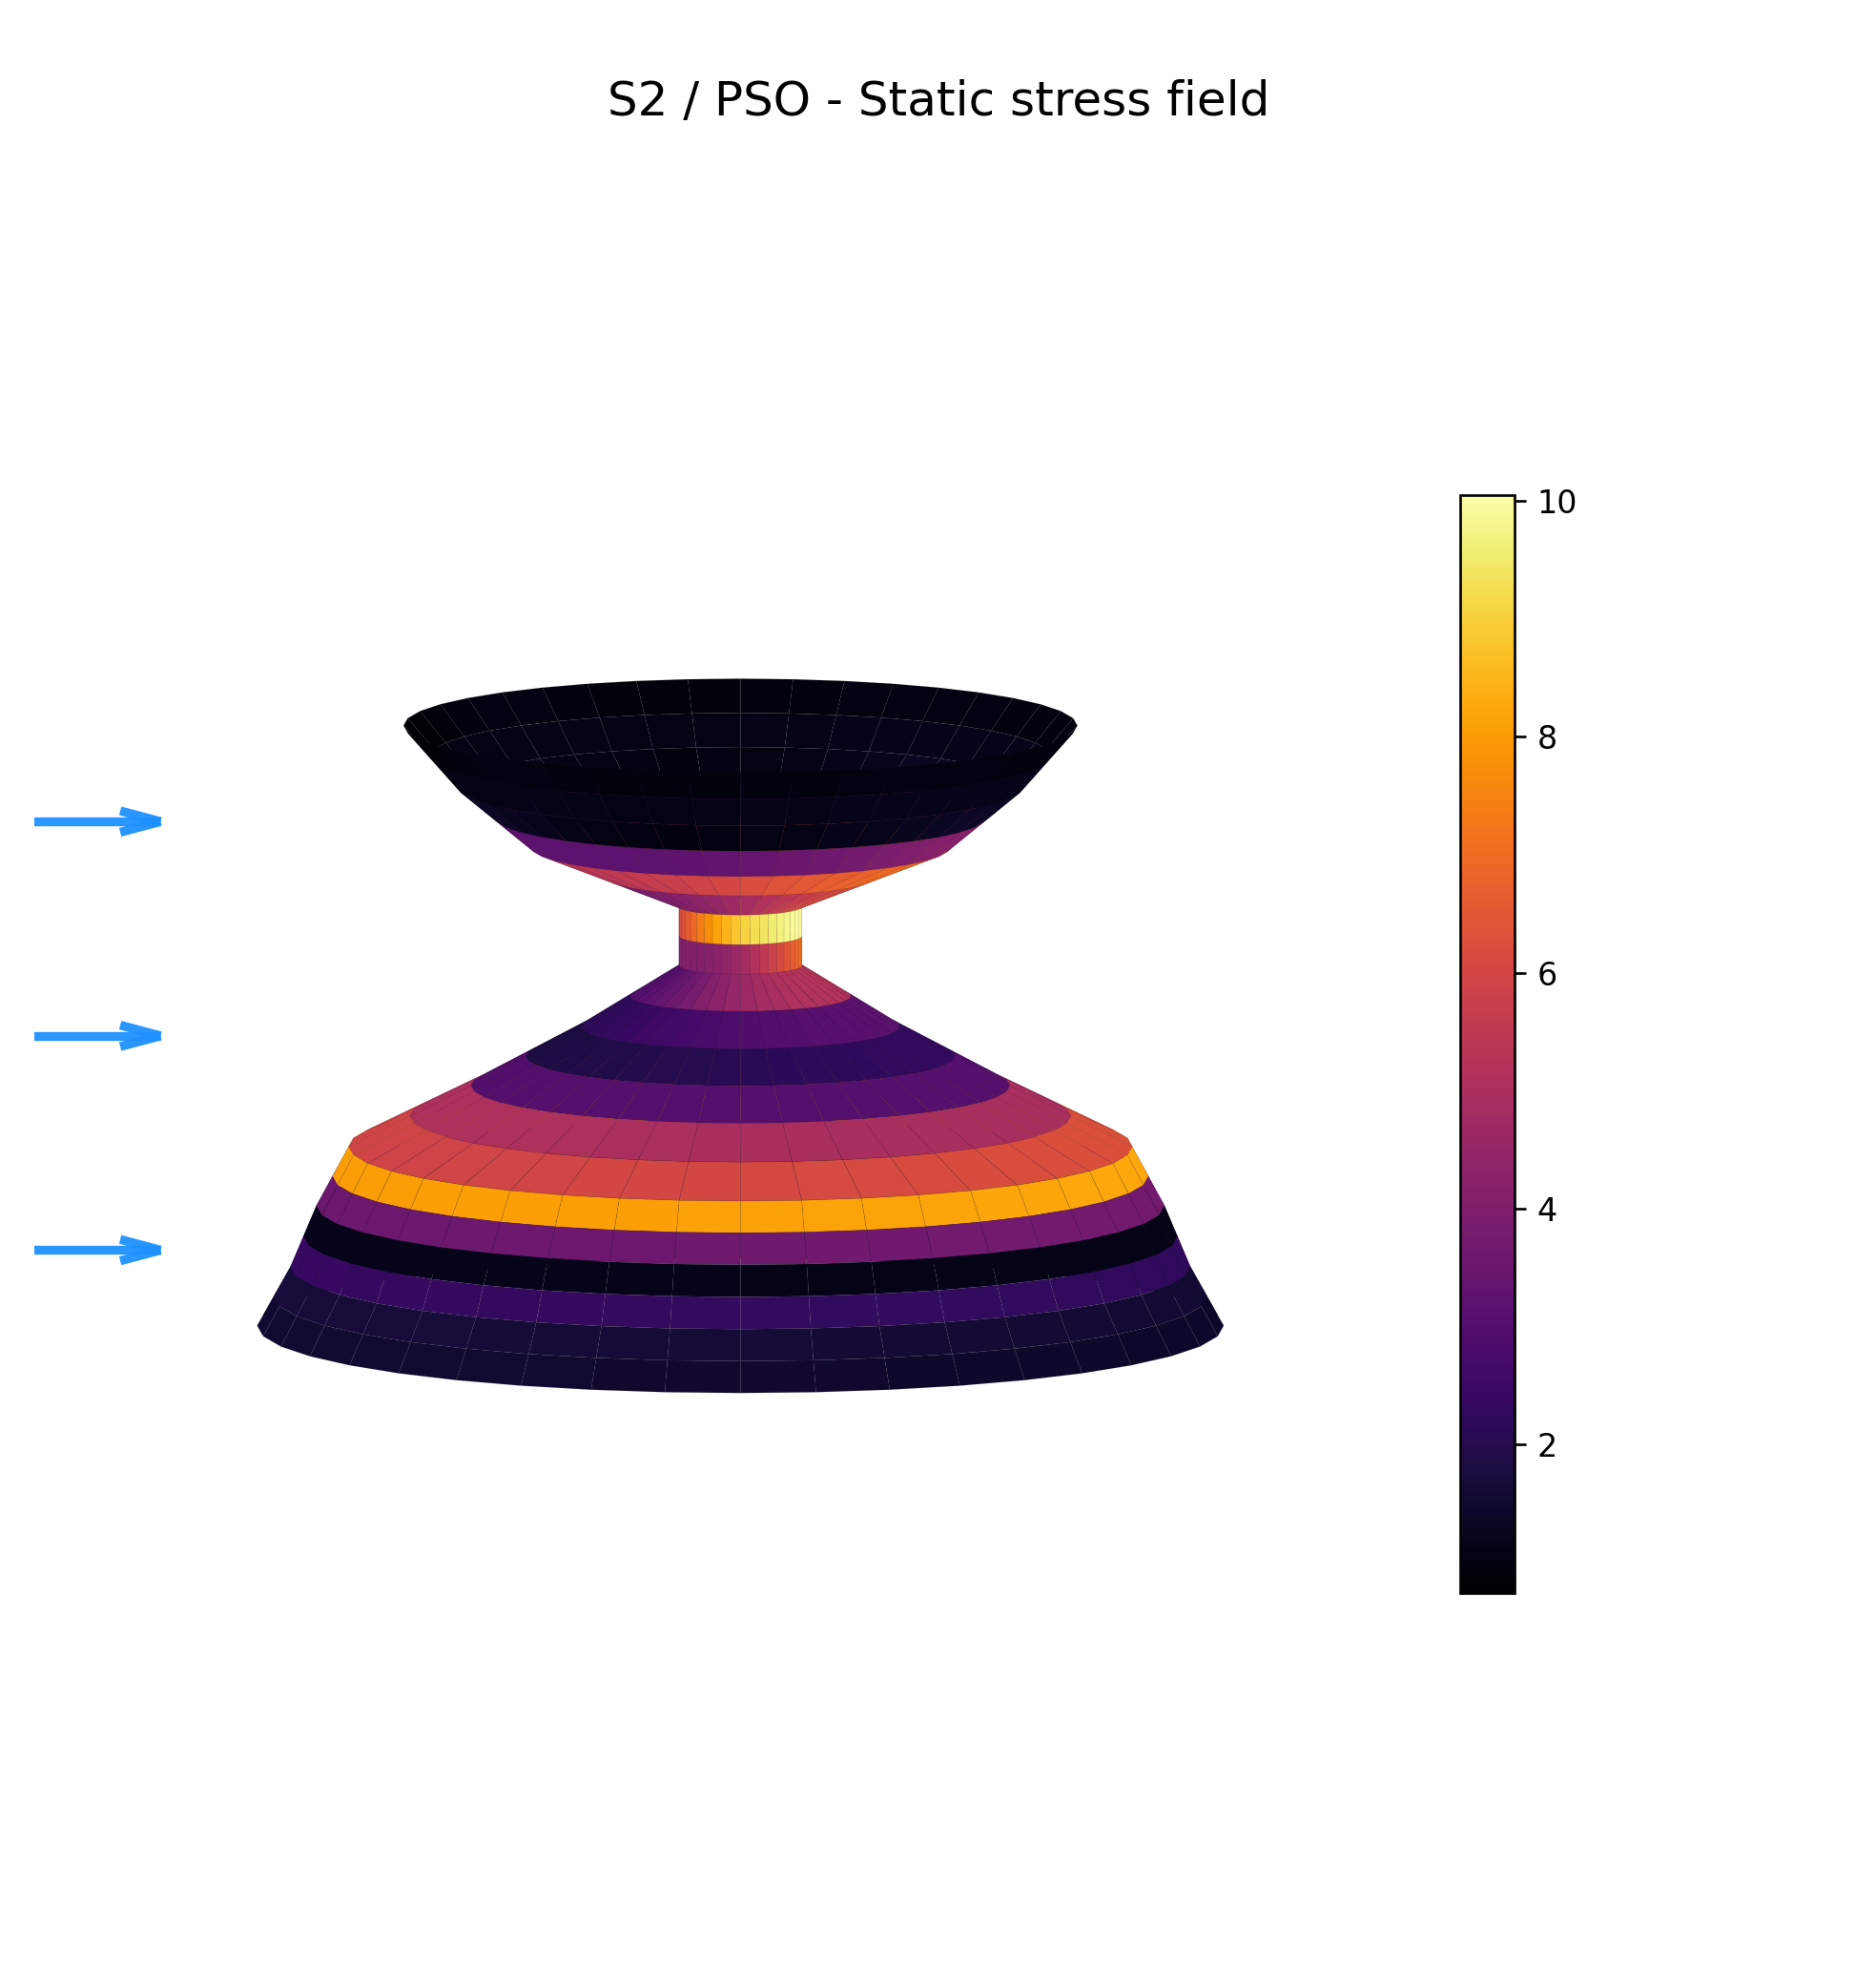
\includegraphics[width=\textwidth]{../results/figures/task7_s2_pso_stress.png}
\caption{S2 / PSO stress}
\end{subfigure}\hfill
\begin{subfigure}{0.32\textwidth}
\centering
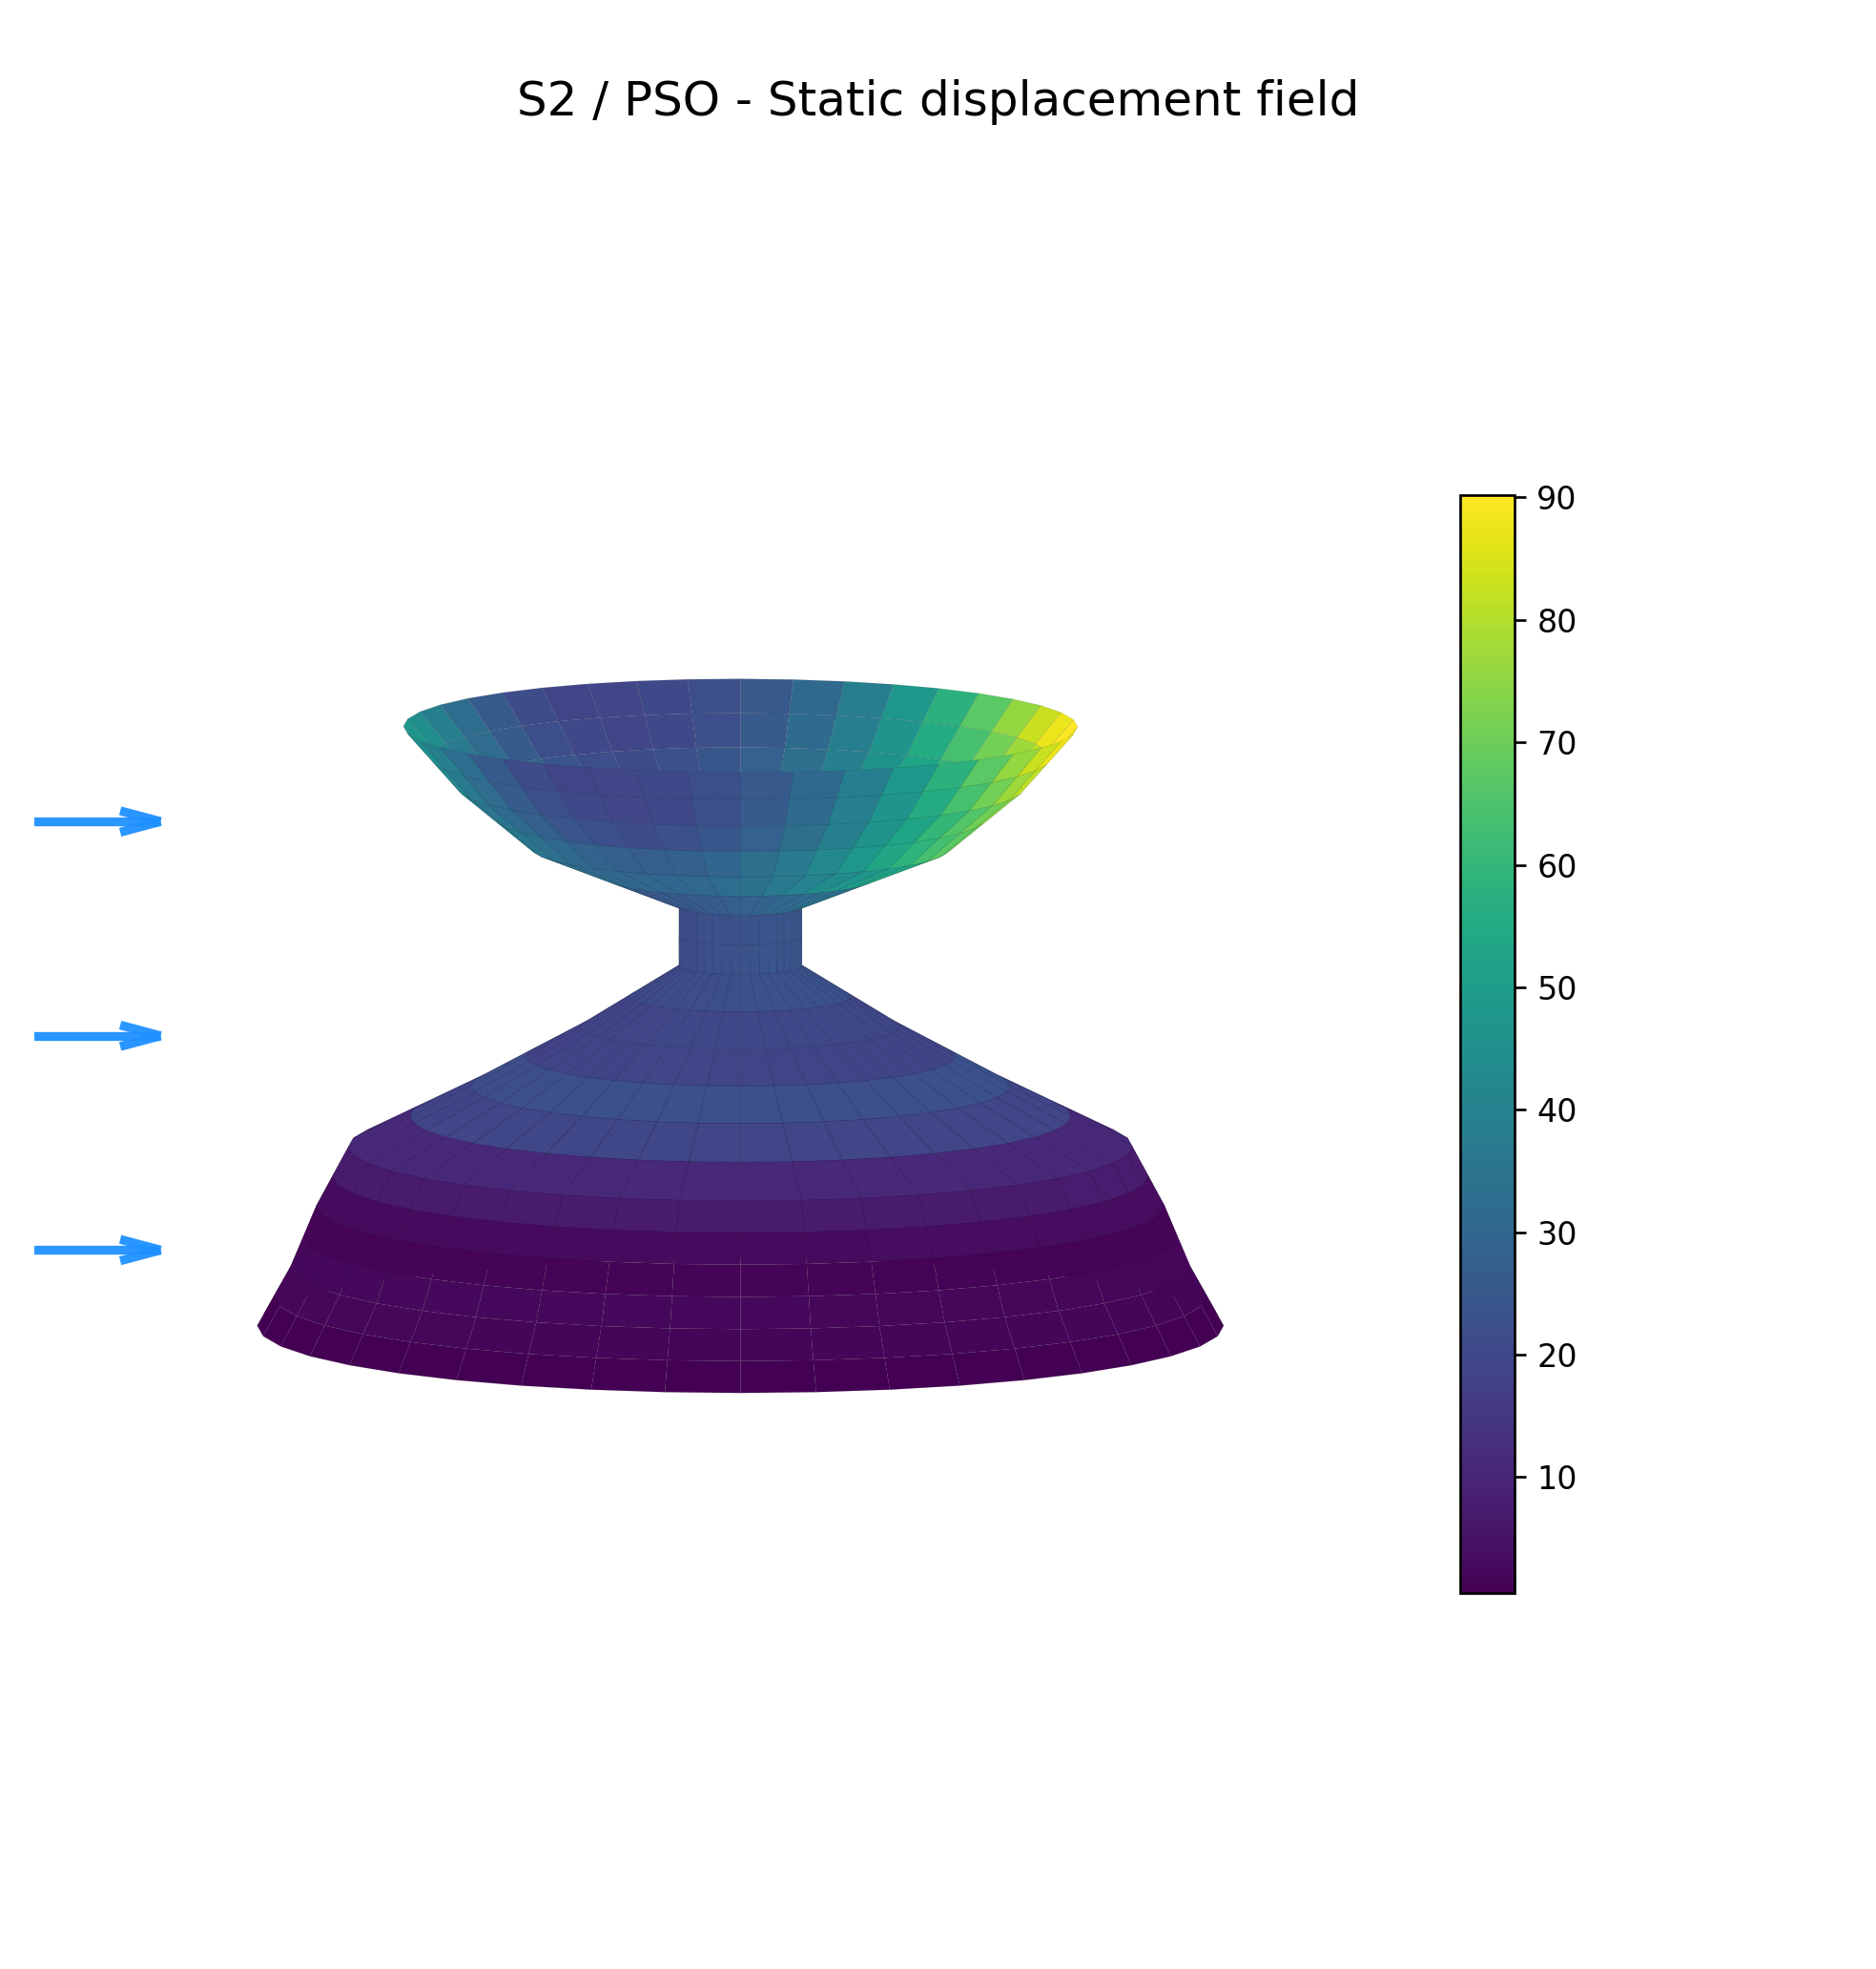
\includegraphics[width=\textwidth]{../results/figures/task7_s2_pso_displacement.png}
\caption{S2 / PSO displacement}
\end{subfigure}\hfill
\begin{subfigure}{0.32\textwidth}
\centering
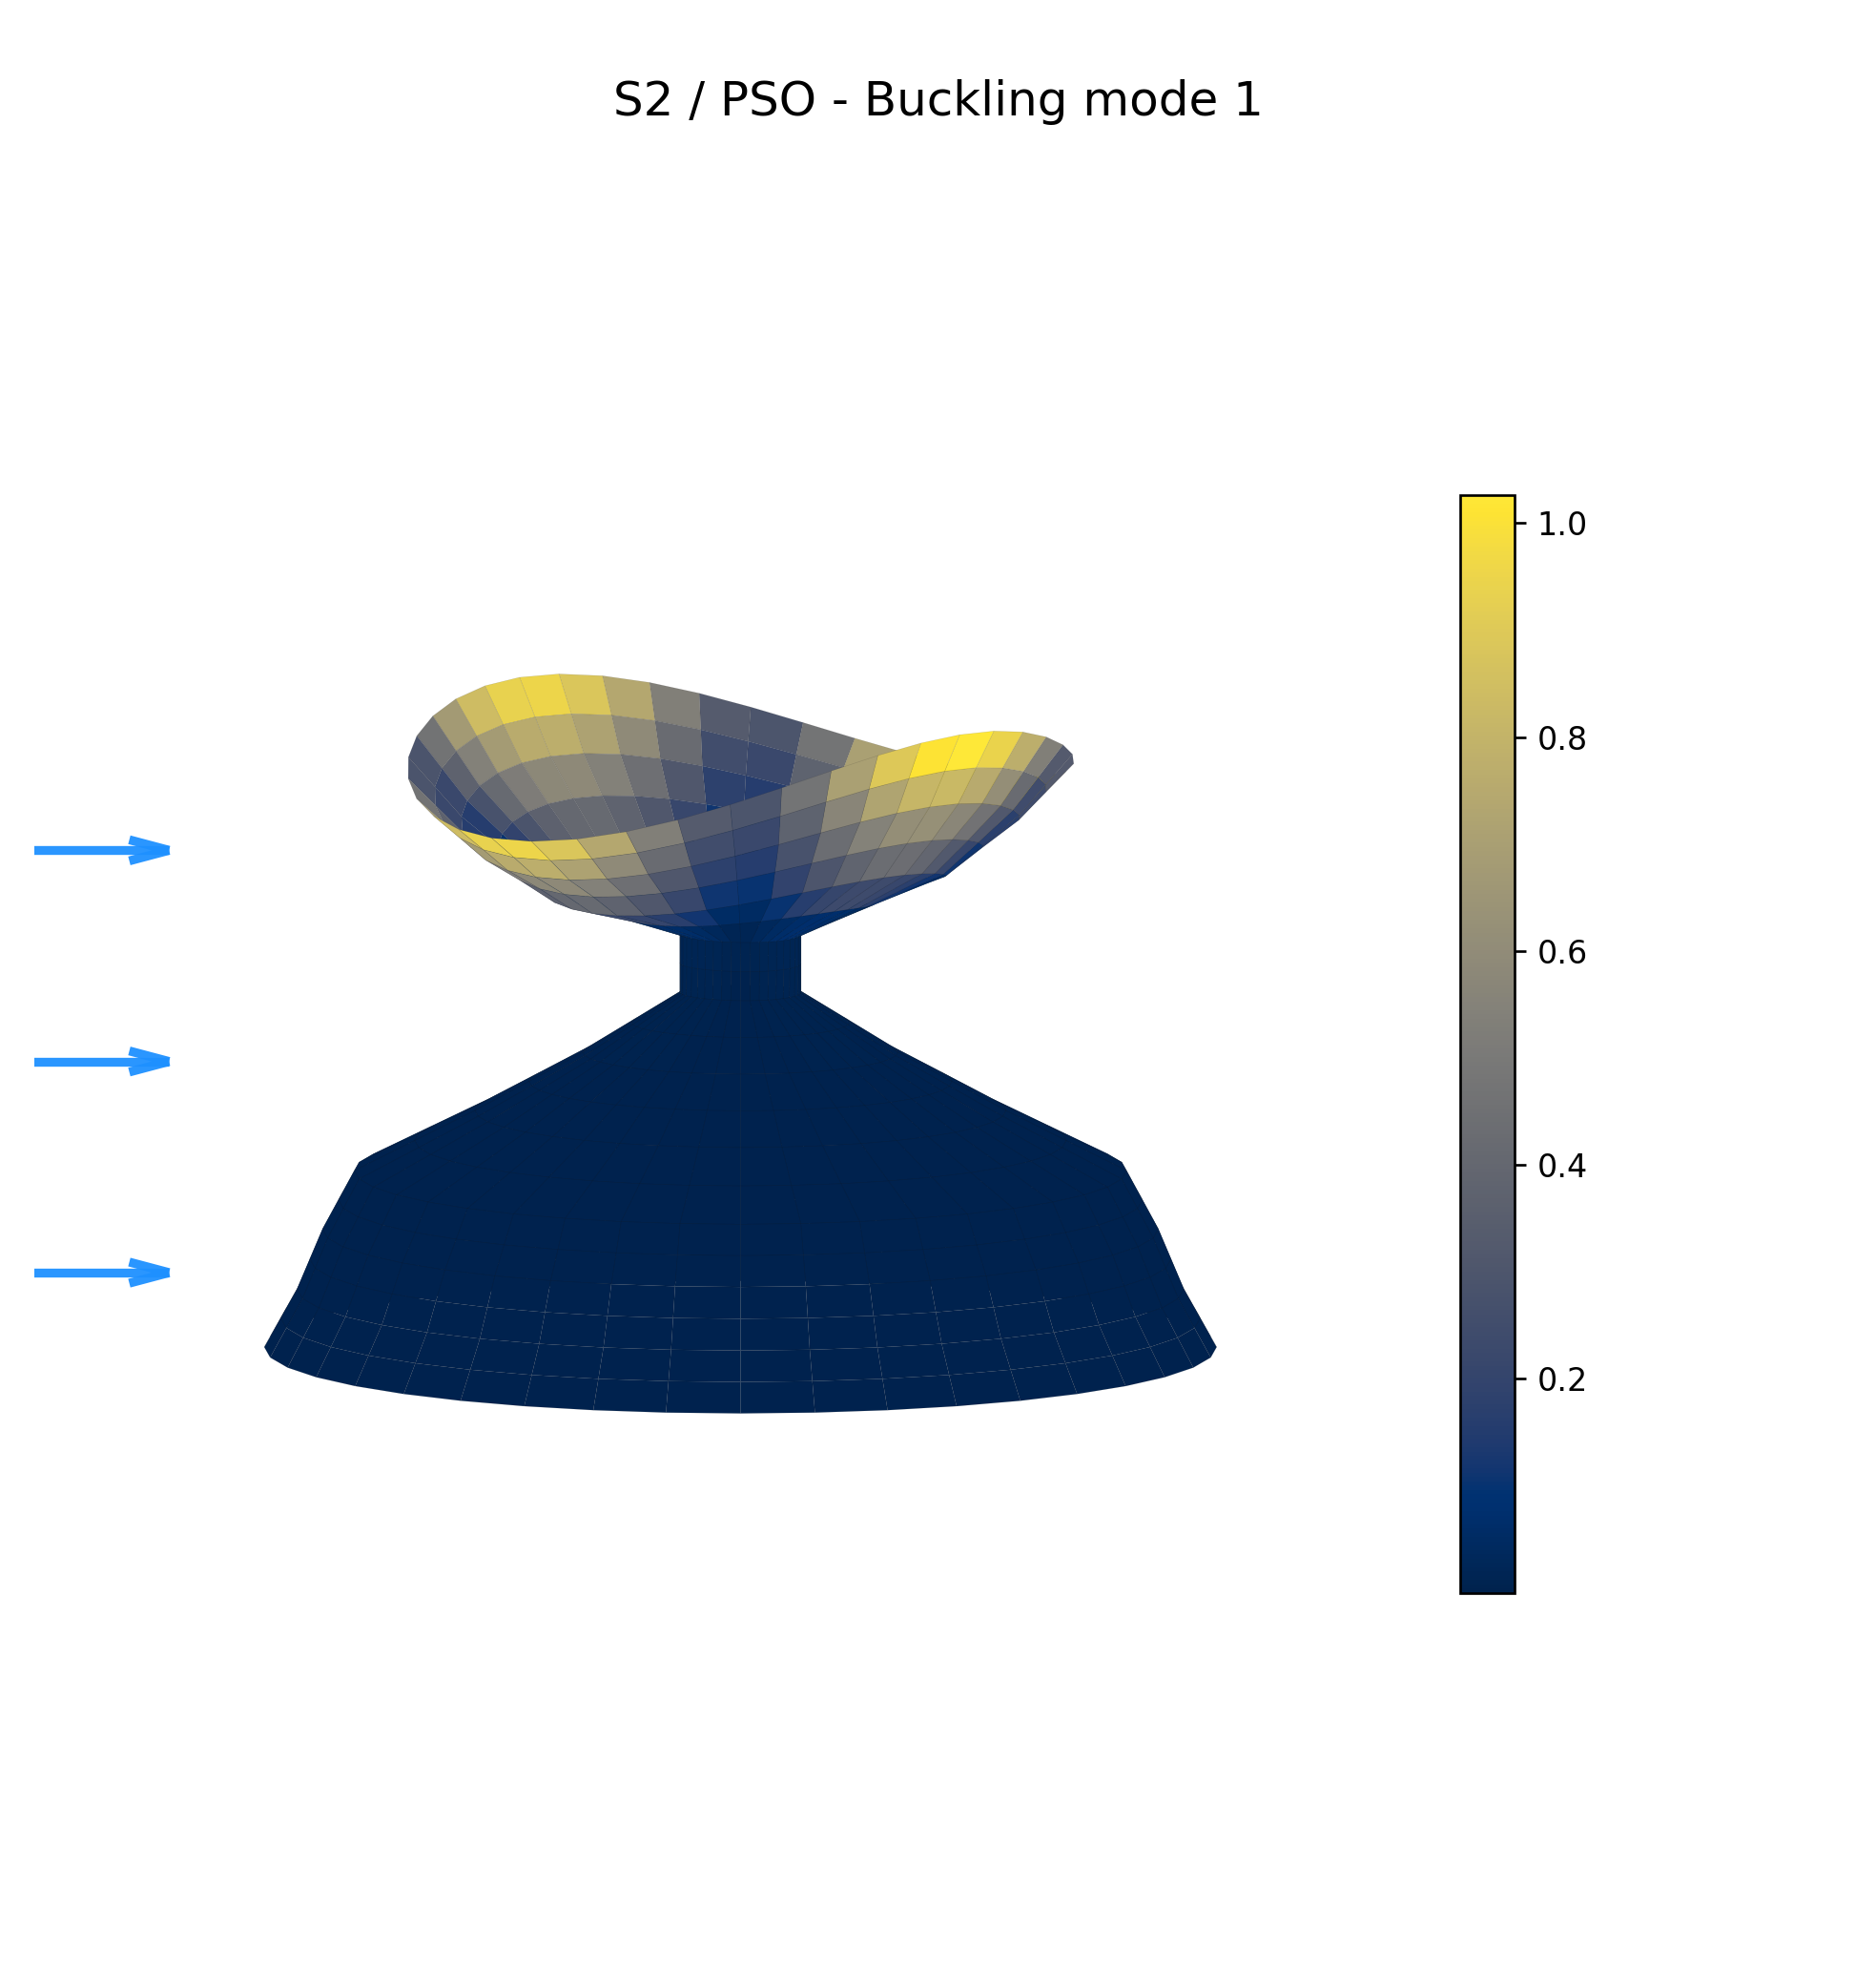
\includegraphics[width=\textwidth]{../results/figures/task7_s2_pso_buckling_mode1.png}
\caption{S2 / PSO buckling}
\end{subfigure}
\caption{Combined visual fields}
\end{figure}


\section{Scenario S3}


\subsection{S3 / BFGS}


\begin{figure}[H]
\centering
\begin{subfigure}{0.32\textwidth}
\centering
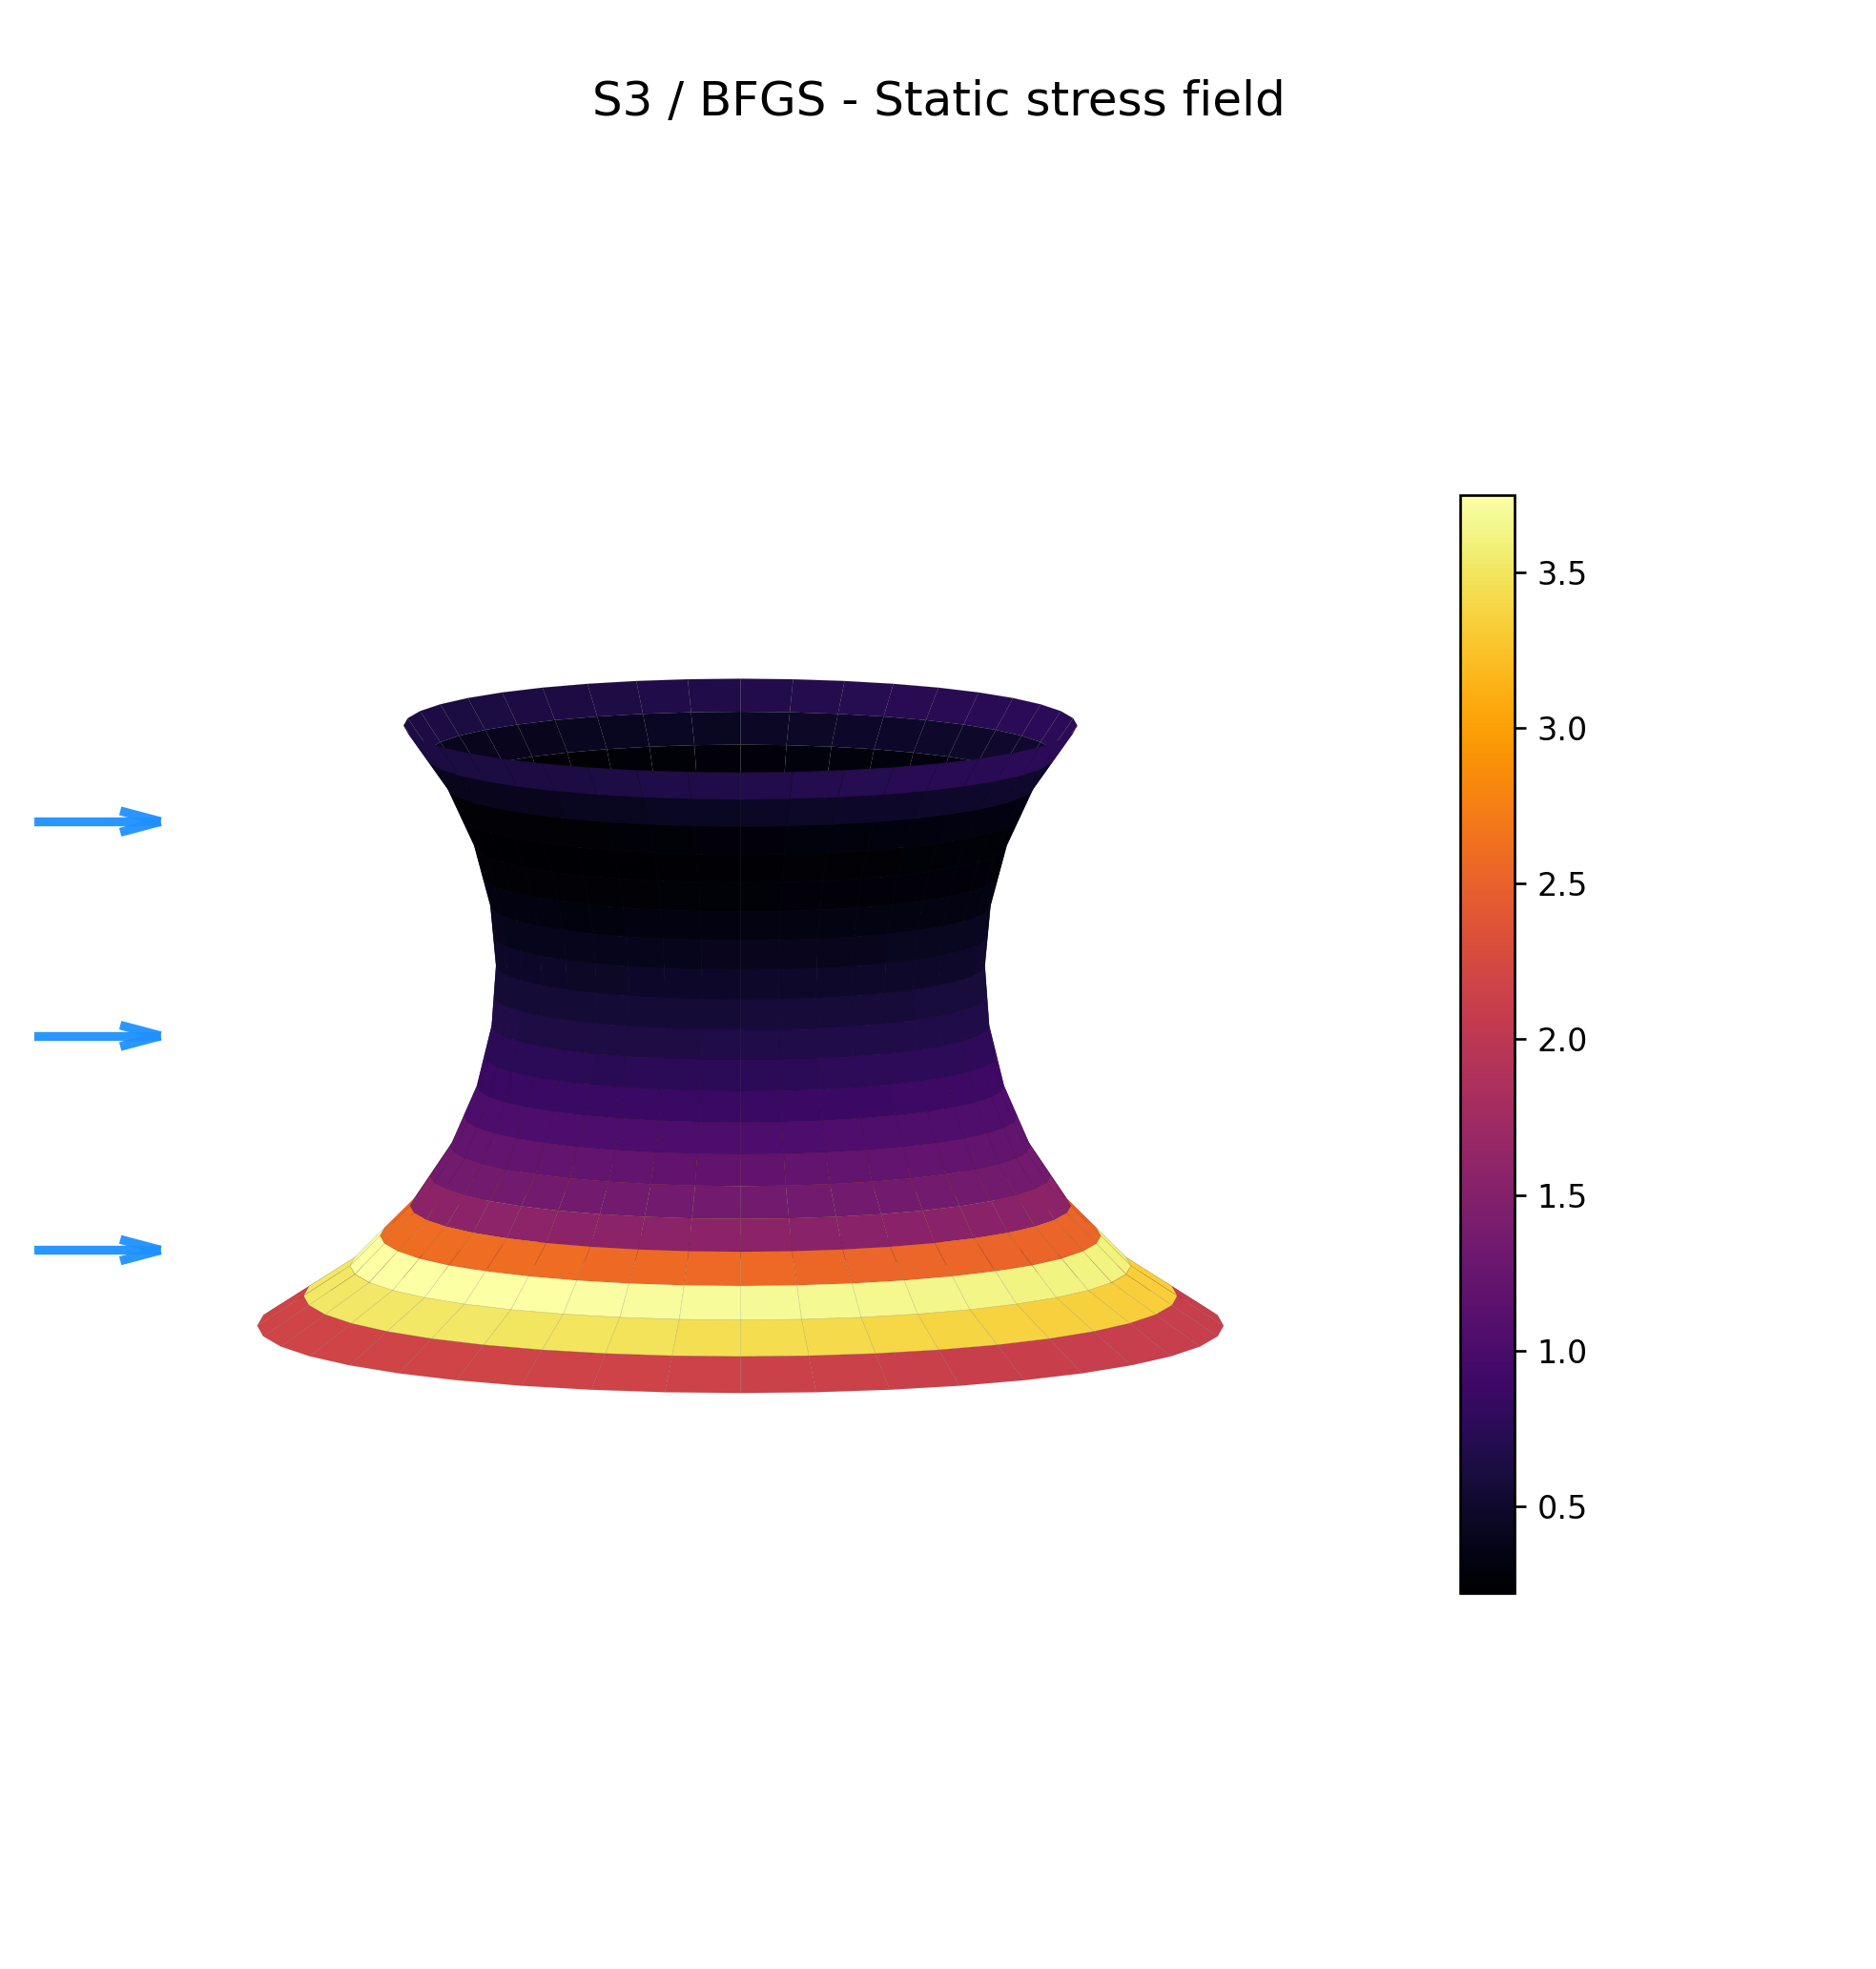
\includegraphics[width=\textwidth]{../results/figures/task7_s3_bfgs_stress.png}
\caption{S3 / BFGS stress}
\end{subfigure}\hfill
\begin{subfigure}{0.32\textwidth}
\centering
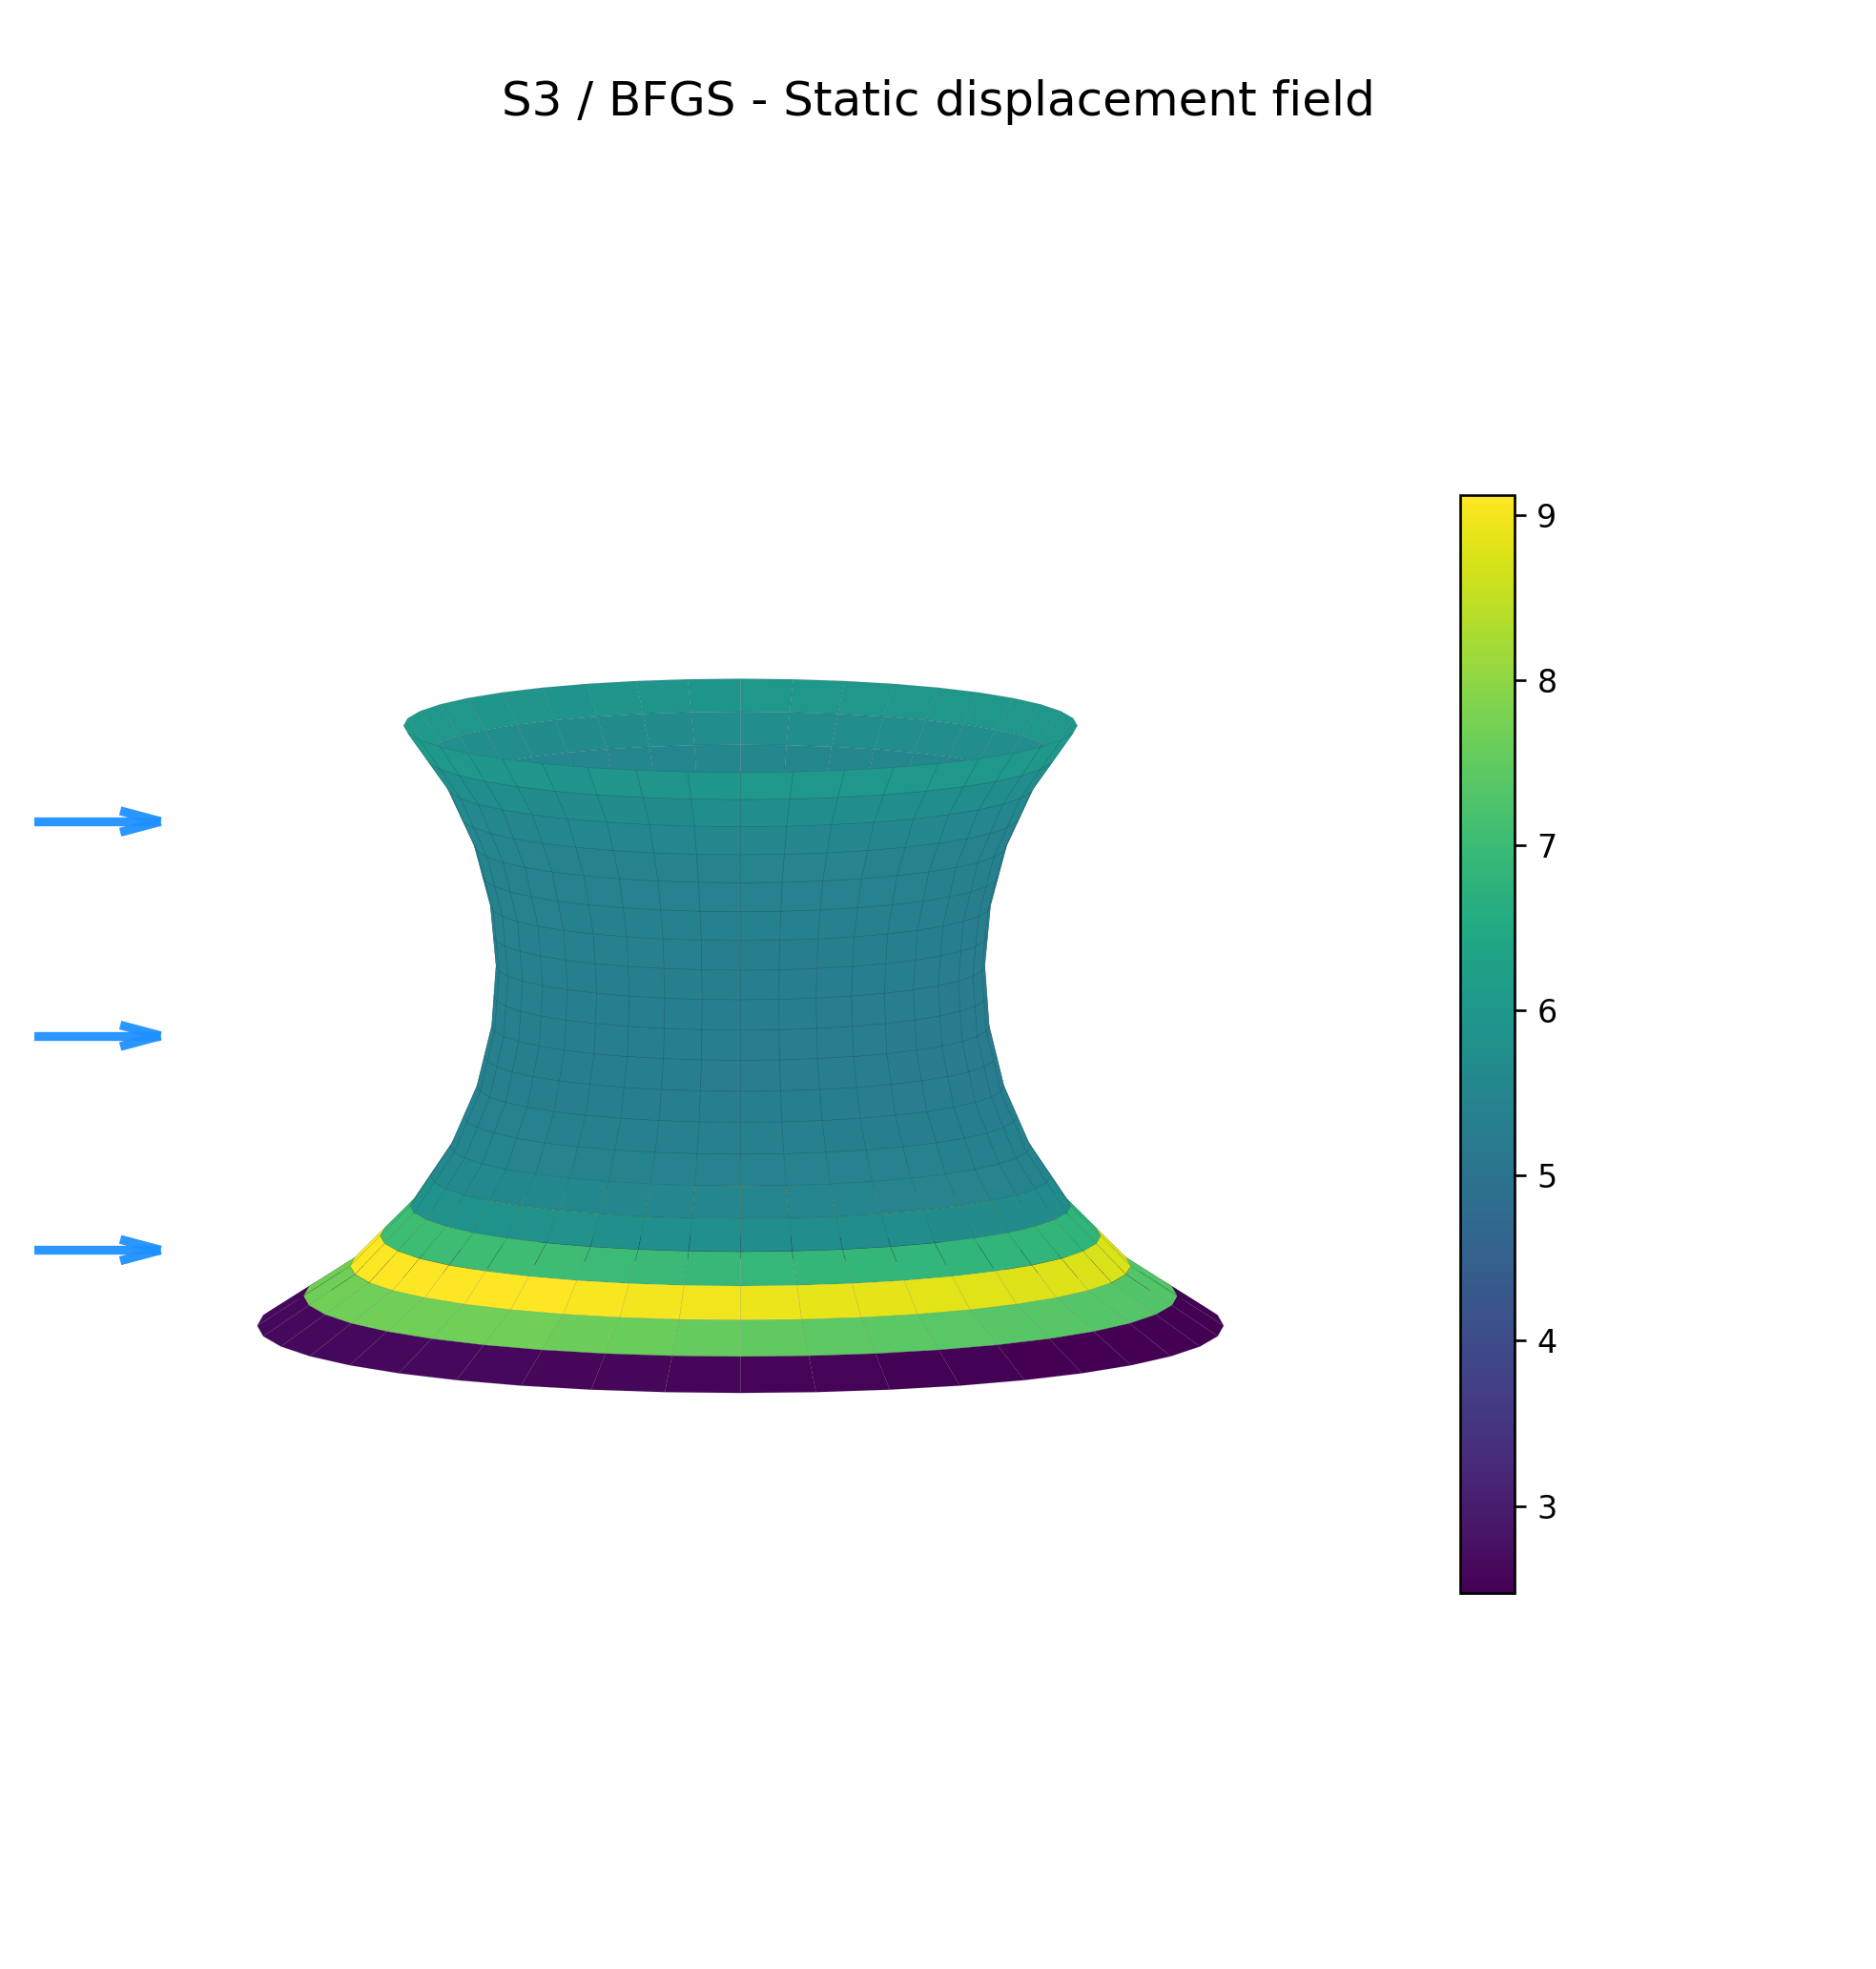
\includegraphics[width=\textwidth]{../results/figures/task7_s3_bfgs_displacement.png}
\caption{S3 / BFGS displacement}
\end{subfigure}\hfill
\begin{subfigure}{0.32\textwidth}
\centering
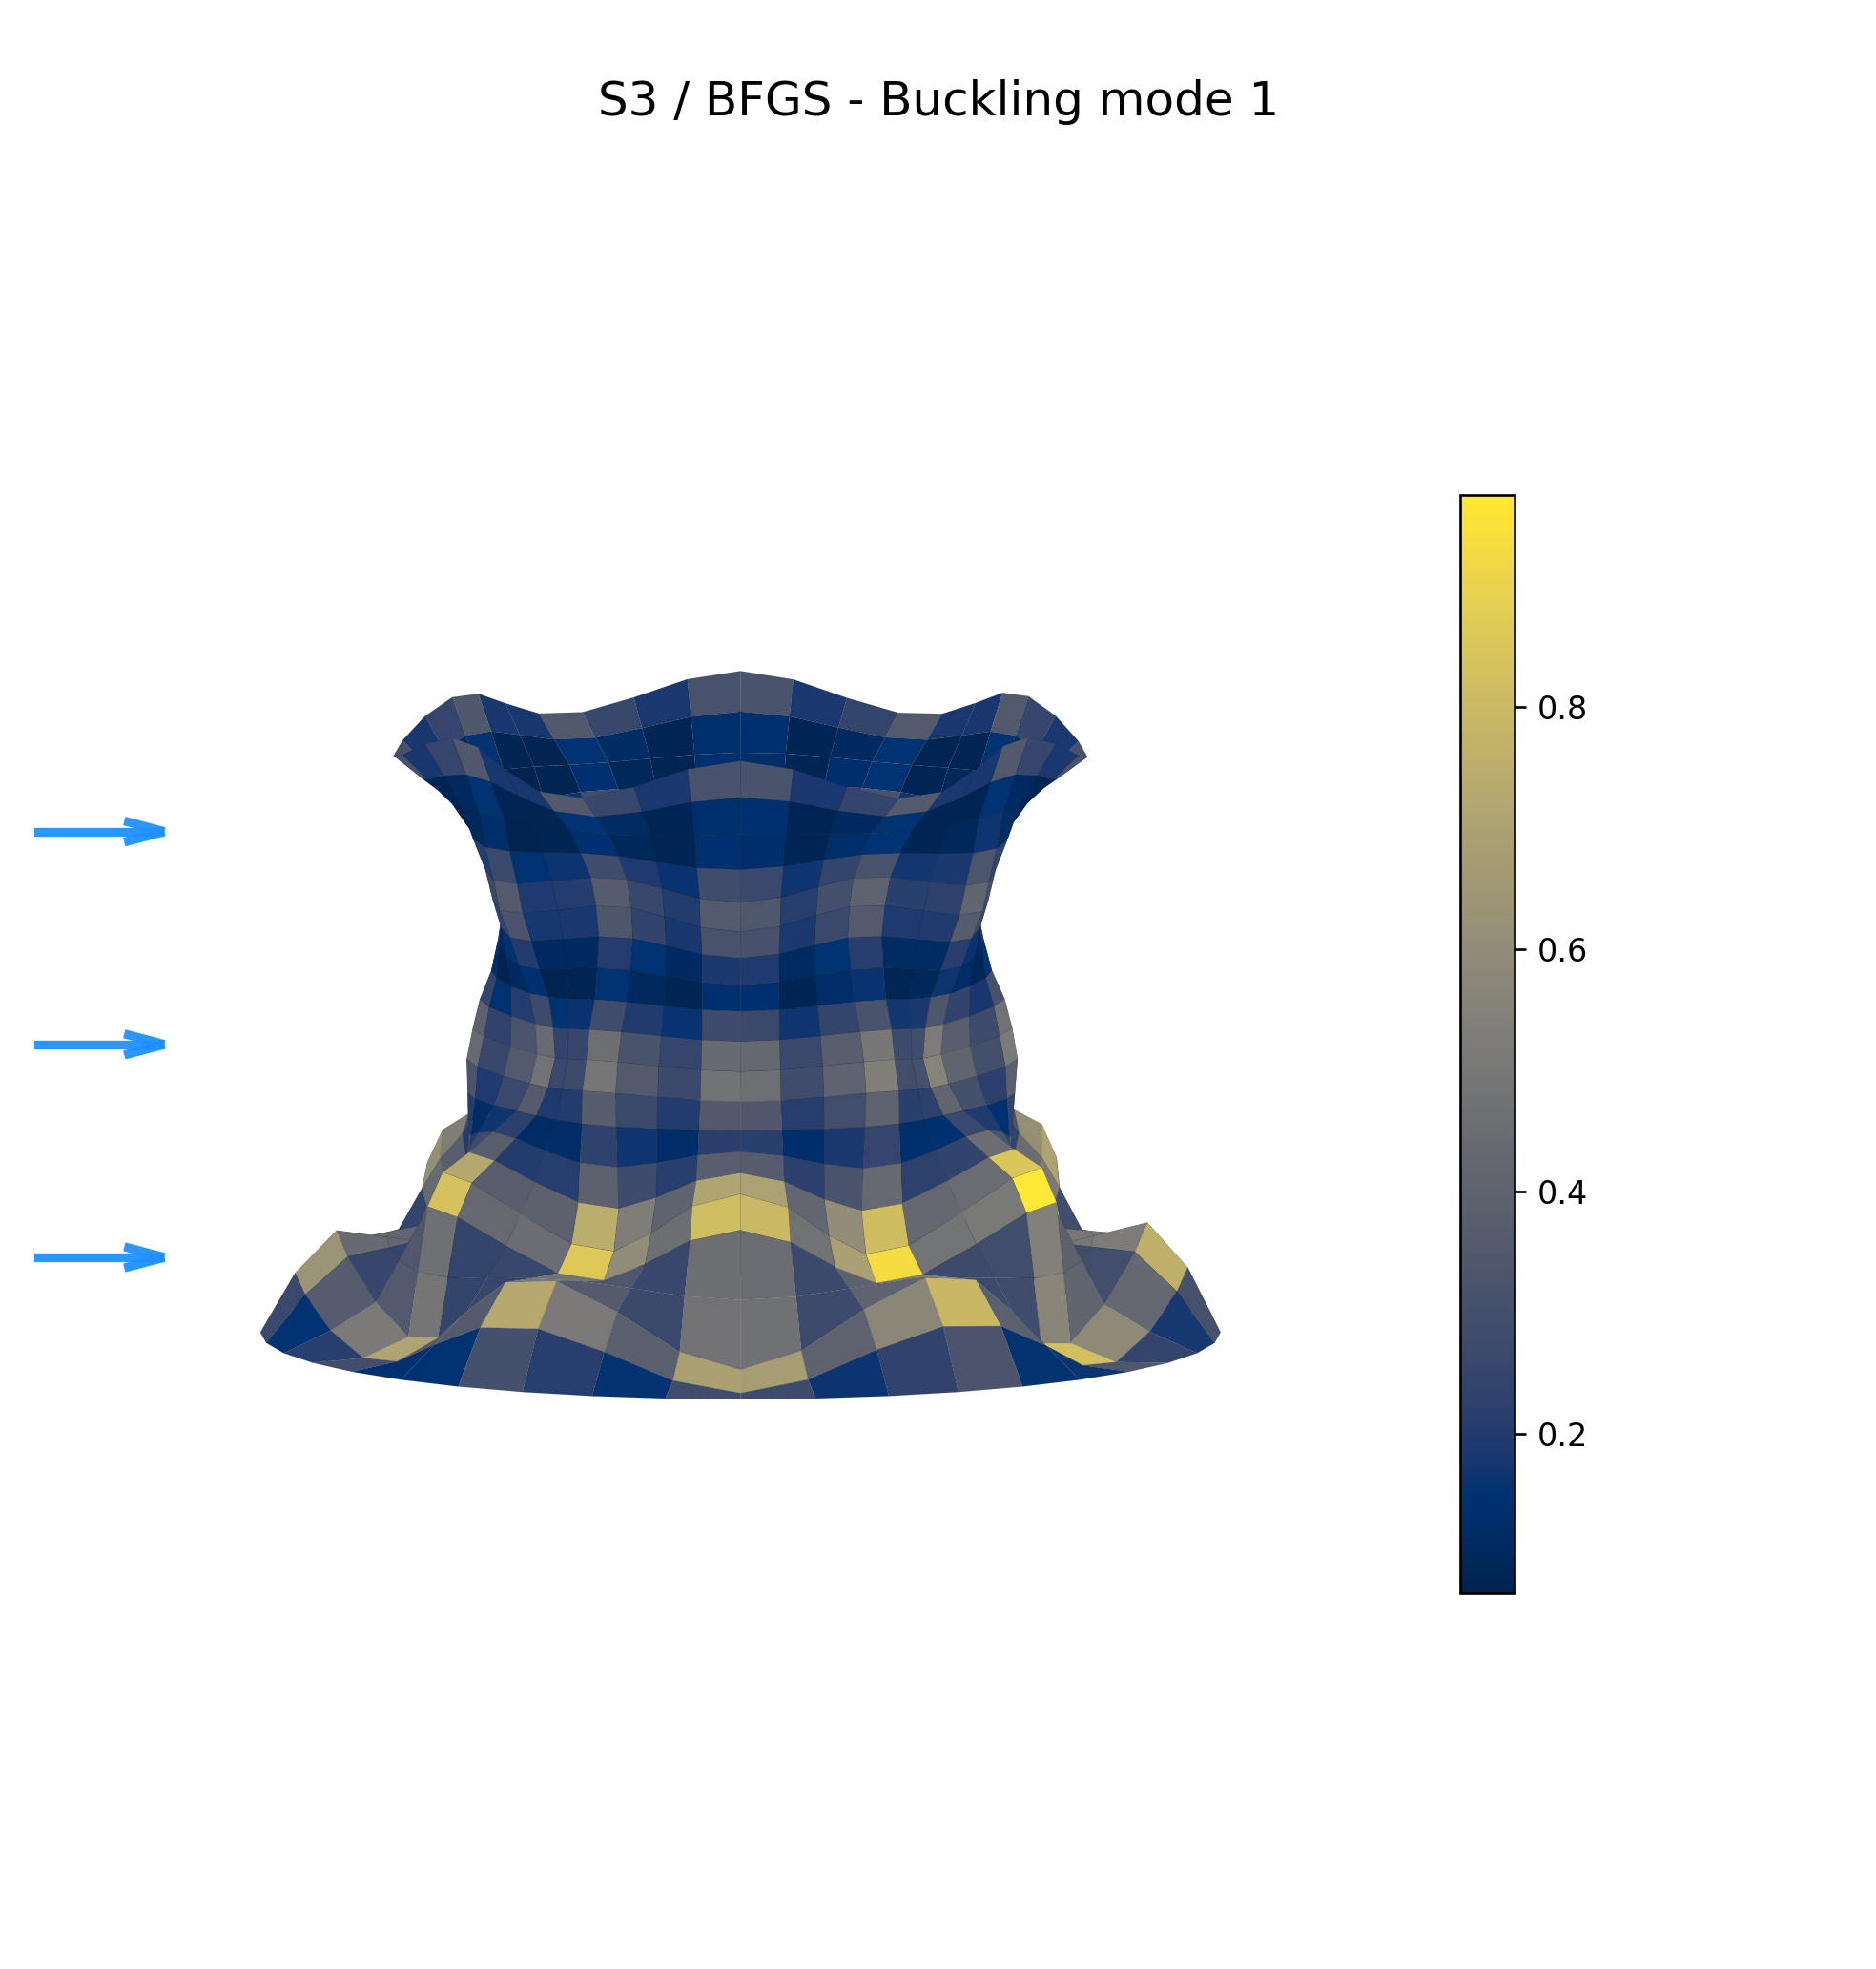
\includegraphics[width=\textwidth]{../results/figures/task7_s3_bfgs_buckling_mode1.png}
\caption{S3 / BFGS buckling}
\end{subfigure}
\caption{Combined visual fields}
\end{figure}


\section{Scenario S4}


\subsection{S4 / BFGS}


\begin{figure}[H]
\centering
\begin{subfigure}{0.32\textwidth}
\centering
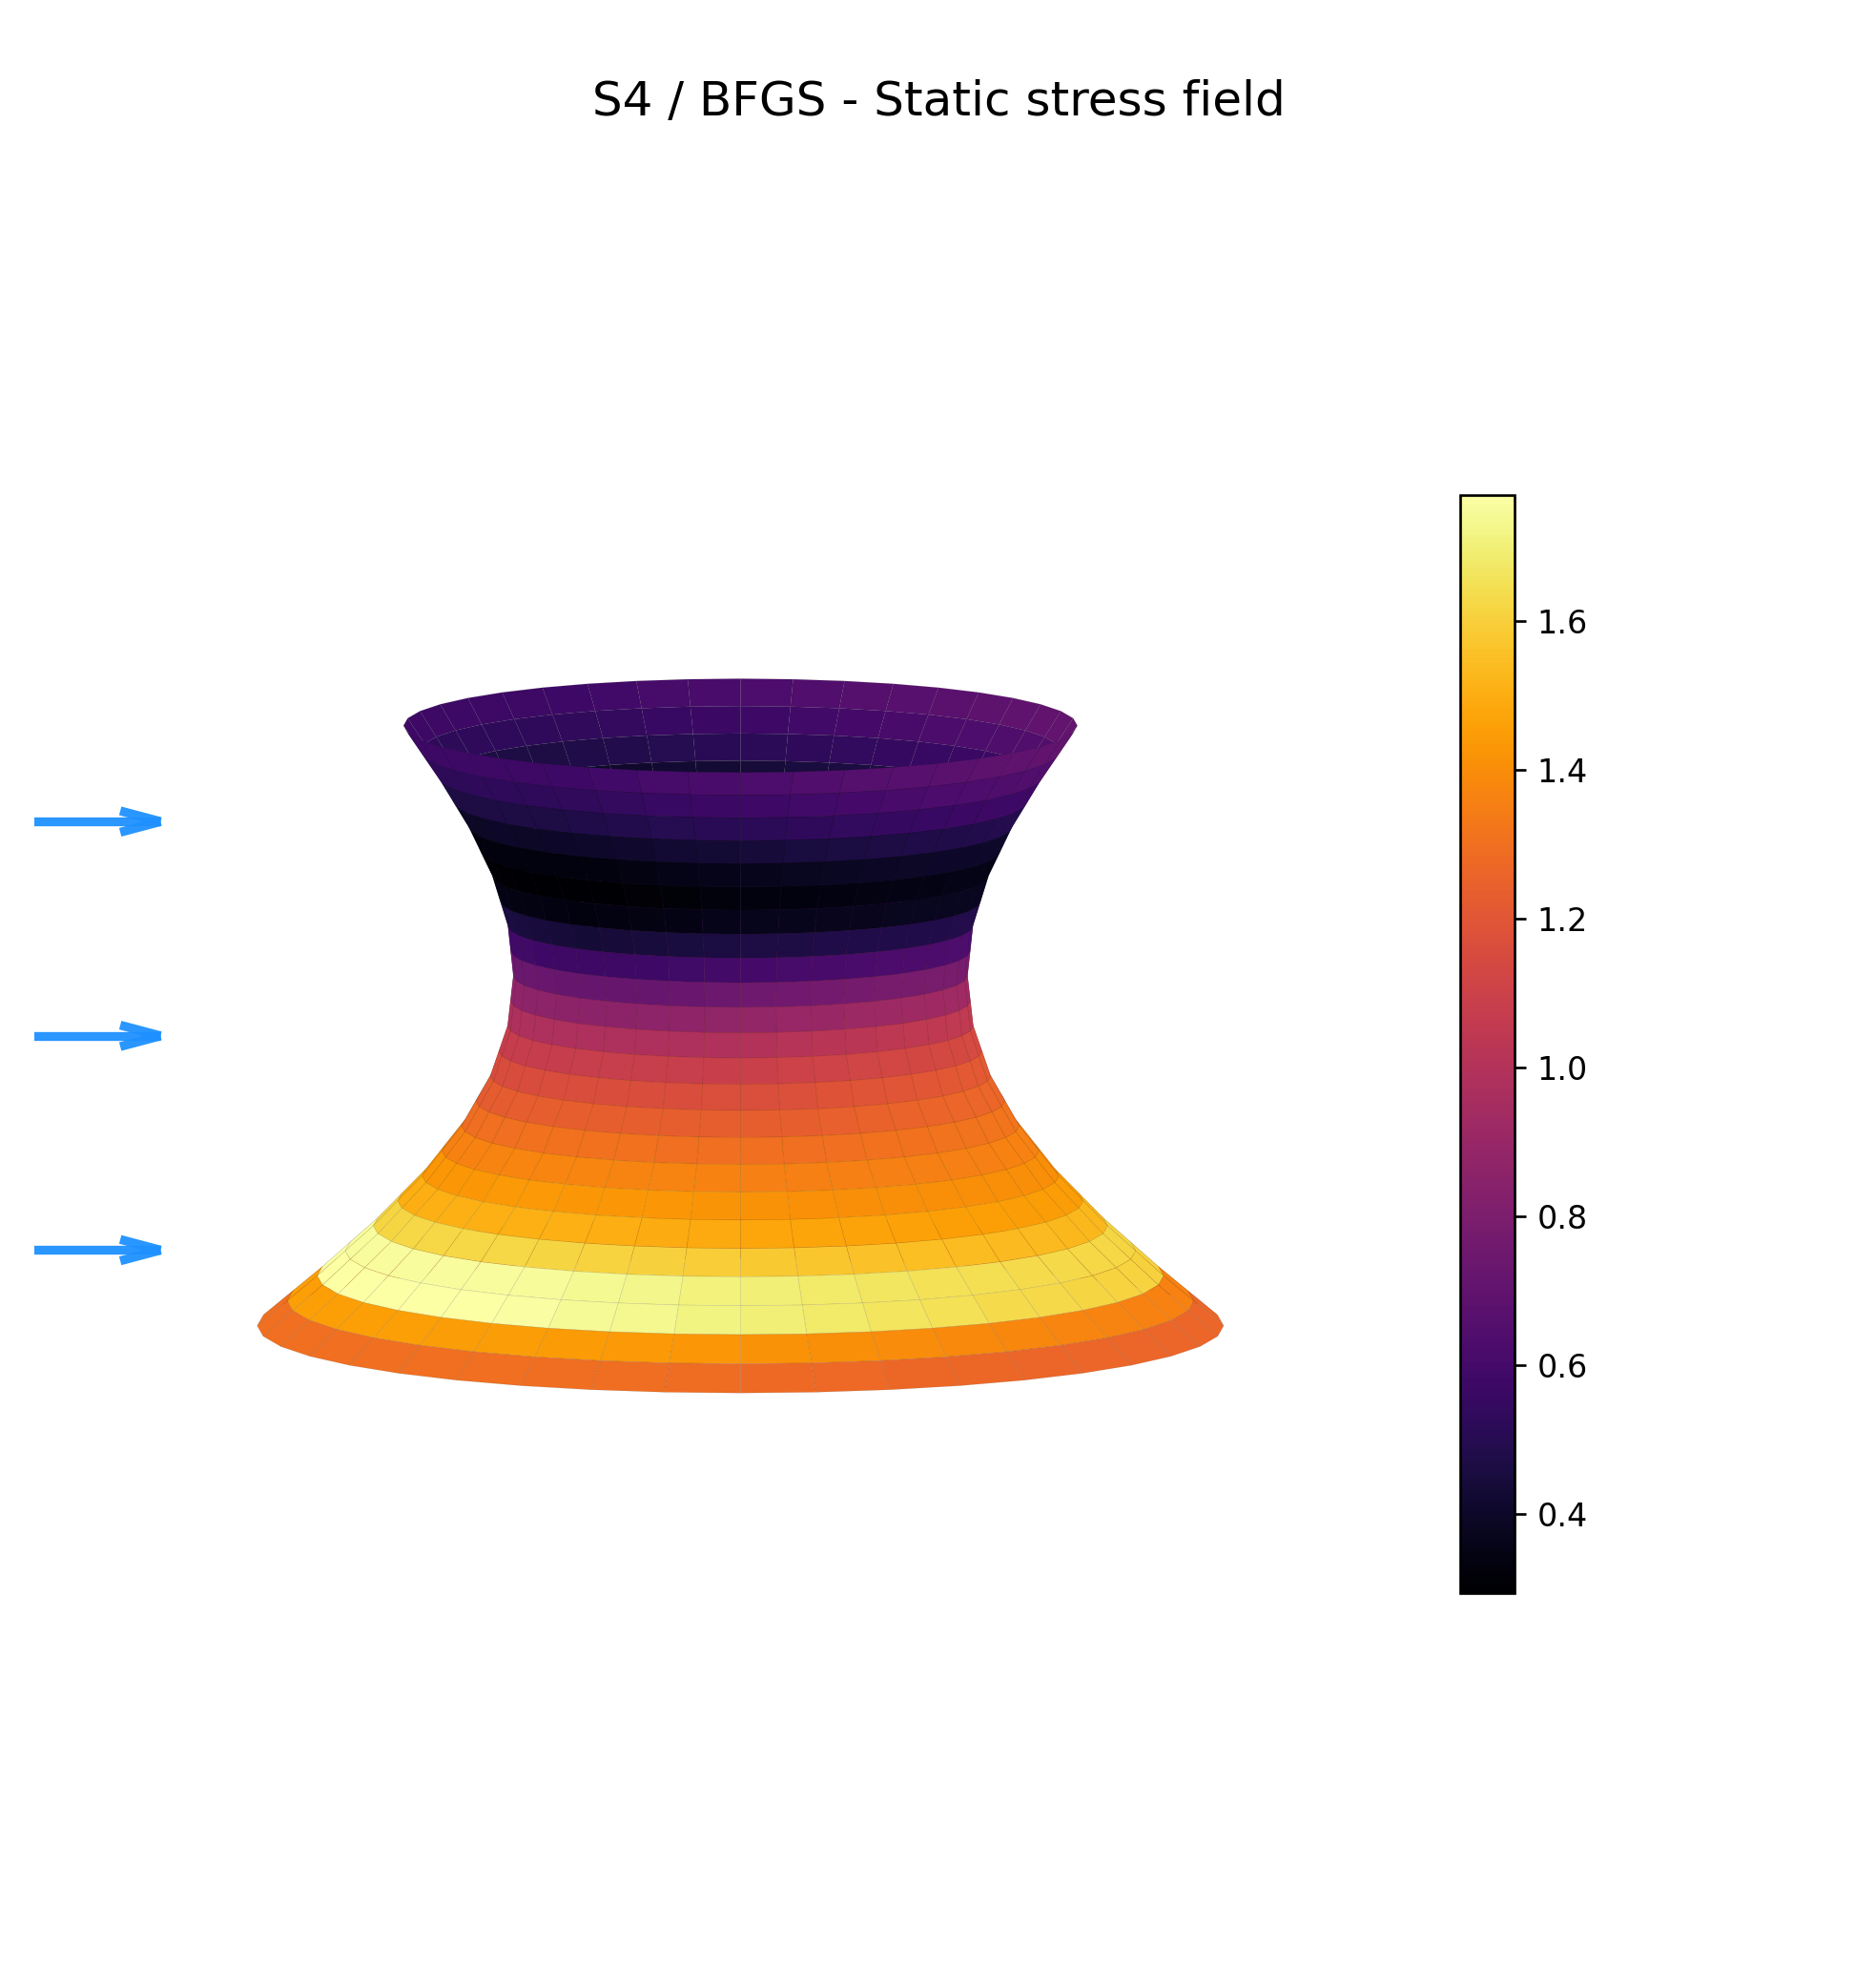
\includegraphics[width=\textwidth]{../results/figures/task7_s4_bfgs_stress.png}
\caption{S4 / BFGS stress}
\end{subfigure}\hfill
\begin{subfigure}{0.32\textwidth}
\centering
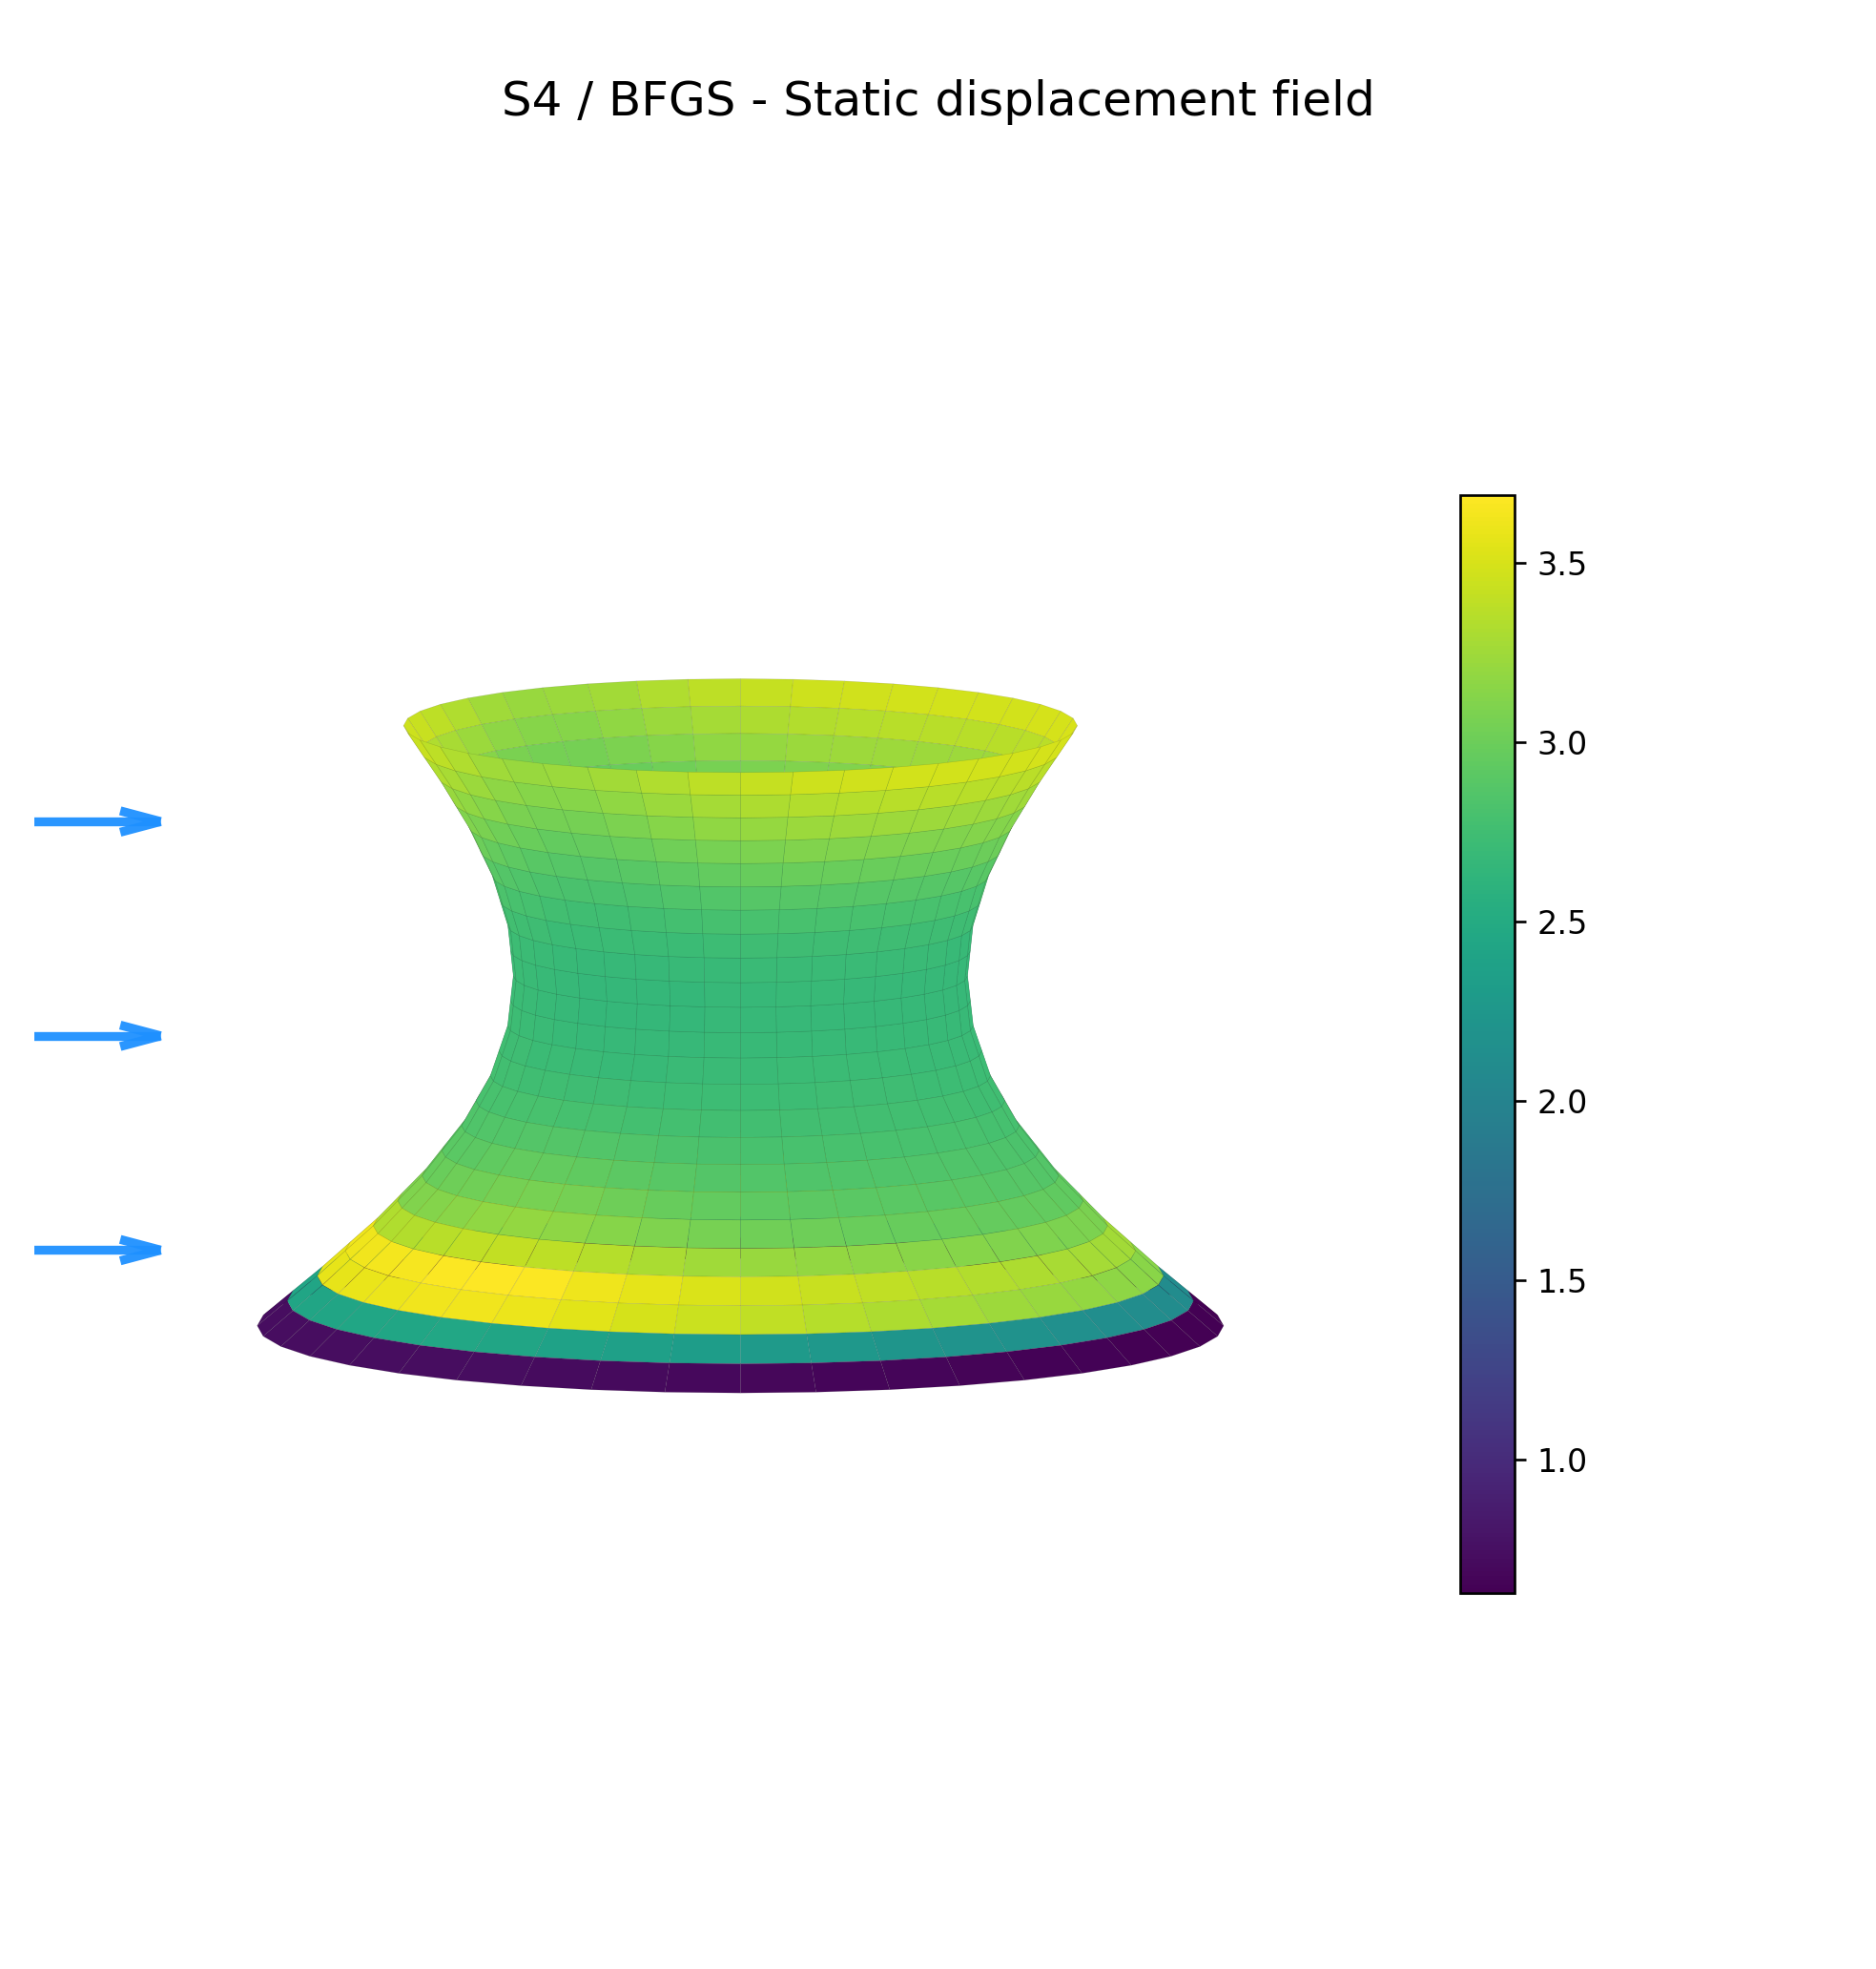
\includegraphics[width=\textwidth]{../results/figures/task7_s4_bfgs_displacement.png}
\caption{S4 / BFGS displacement}
\end{subfigure}\hfill
\begin{subfigure}{0.32\textwidth}
\centering
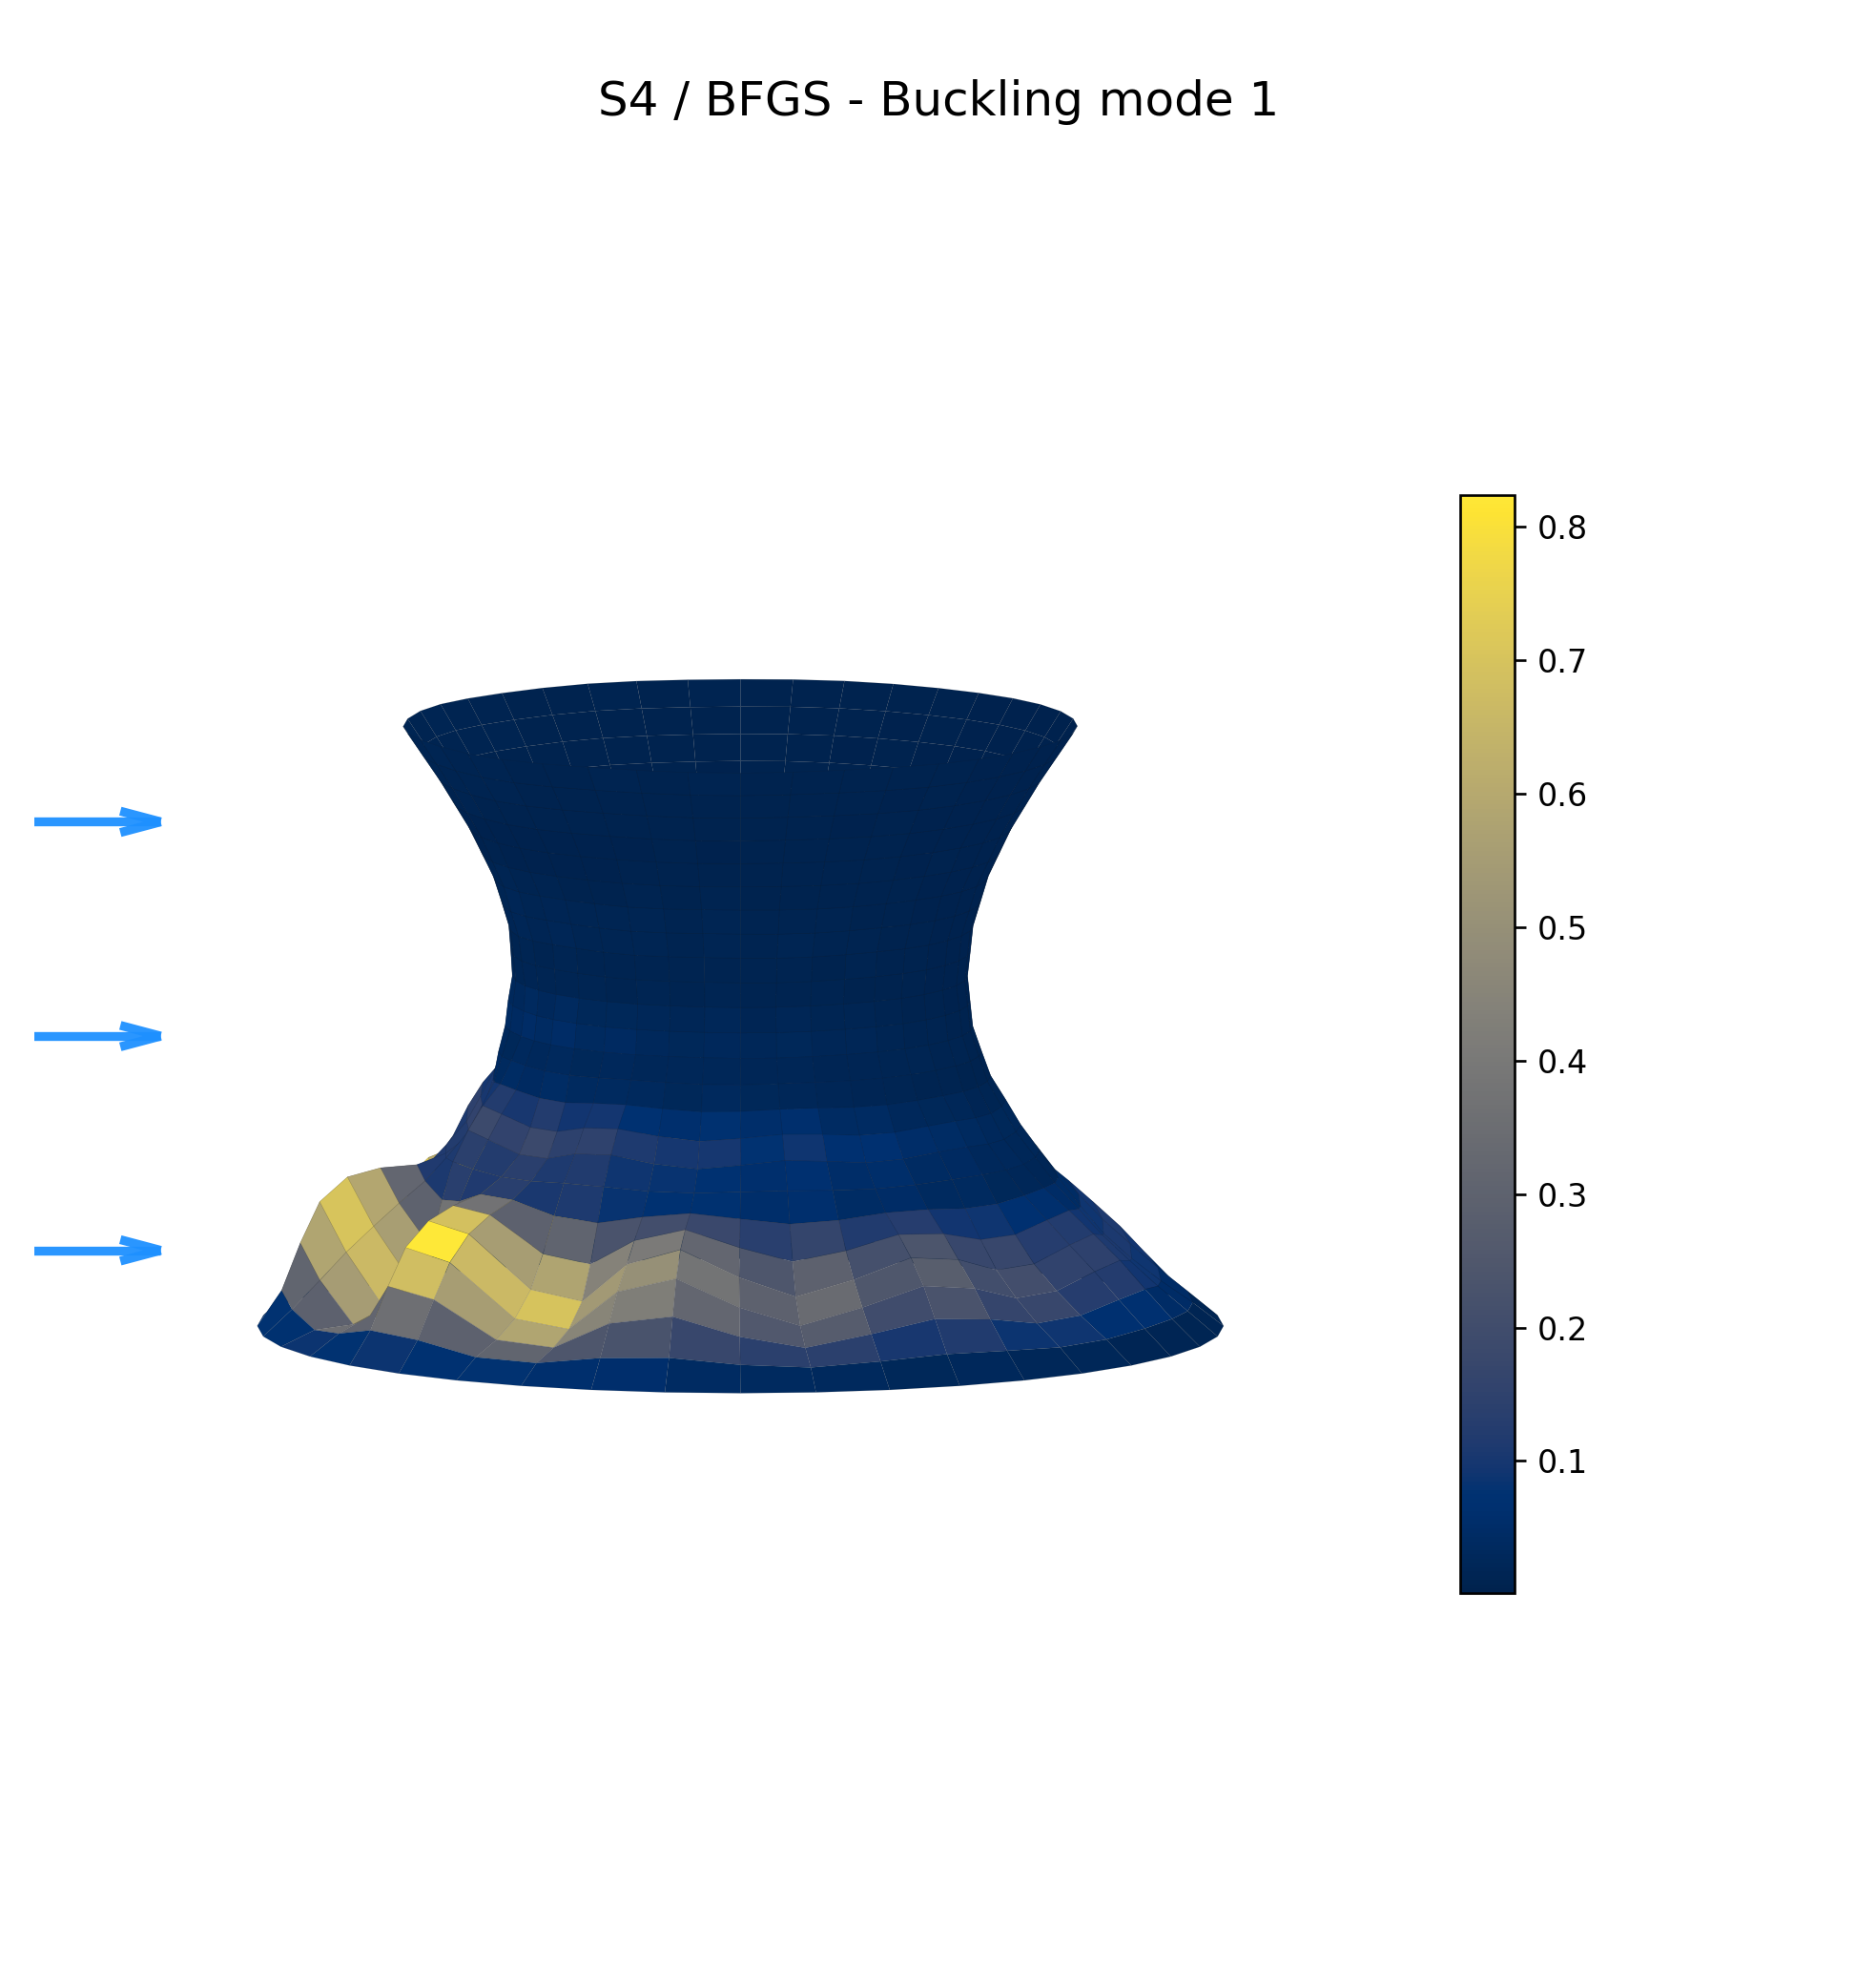
\includegraphics[width=\textwidth]{../results/figures/task7_s4_bfgs_buckling_mode1.png}
\caption{S4 / BFGS buckling}
\end{subfigure}
\caption{Combined visual fields}
\end{figure}


\subsection{S4 / PSO}


\begin{figure}[H]
\centering
\begin{subfigure}{0.32\textwidth}
\centering
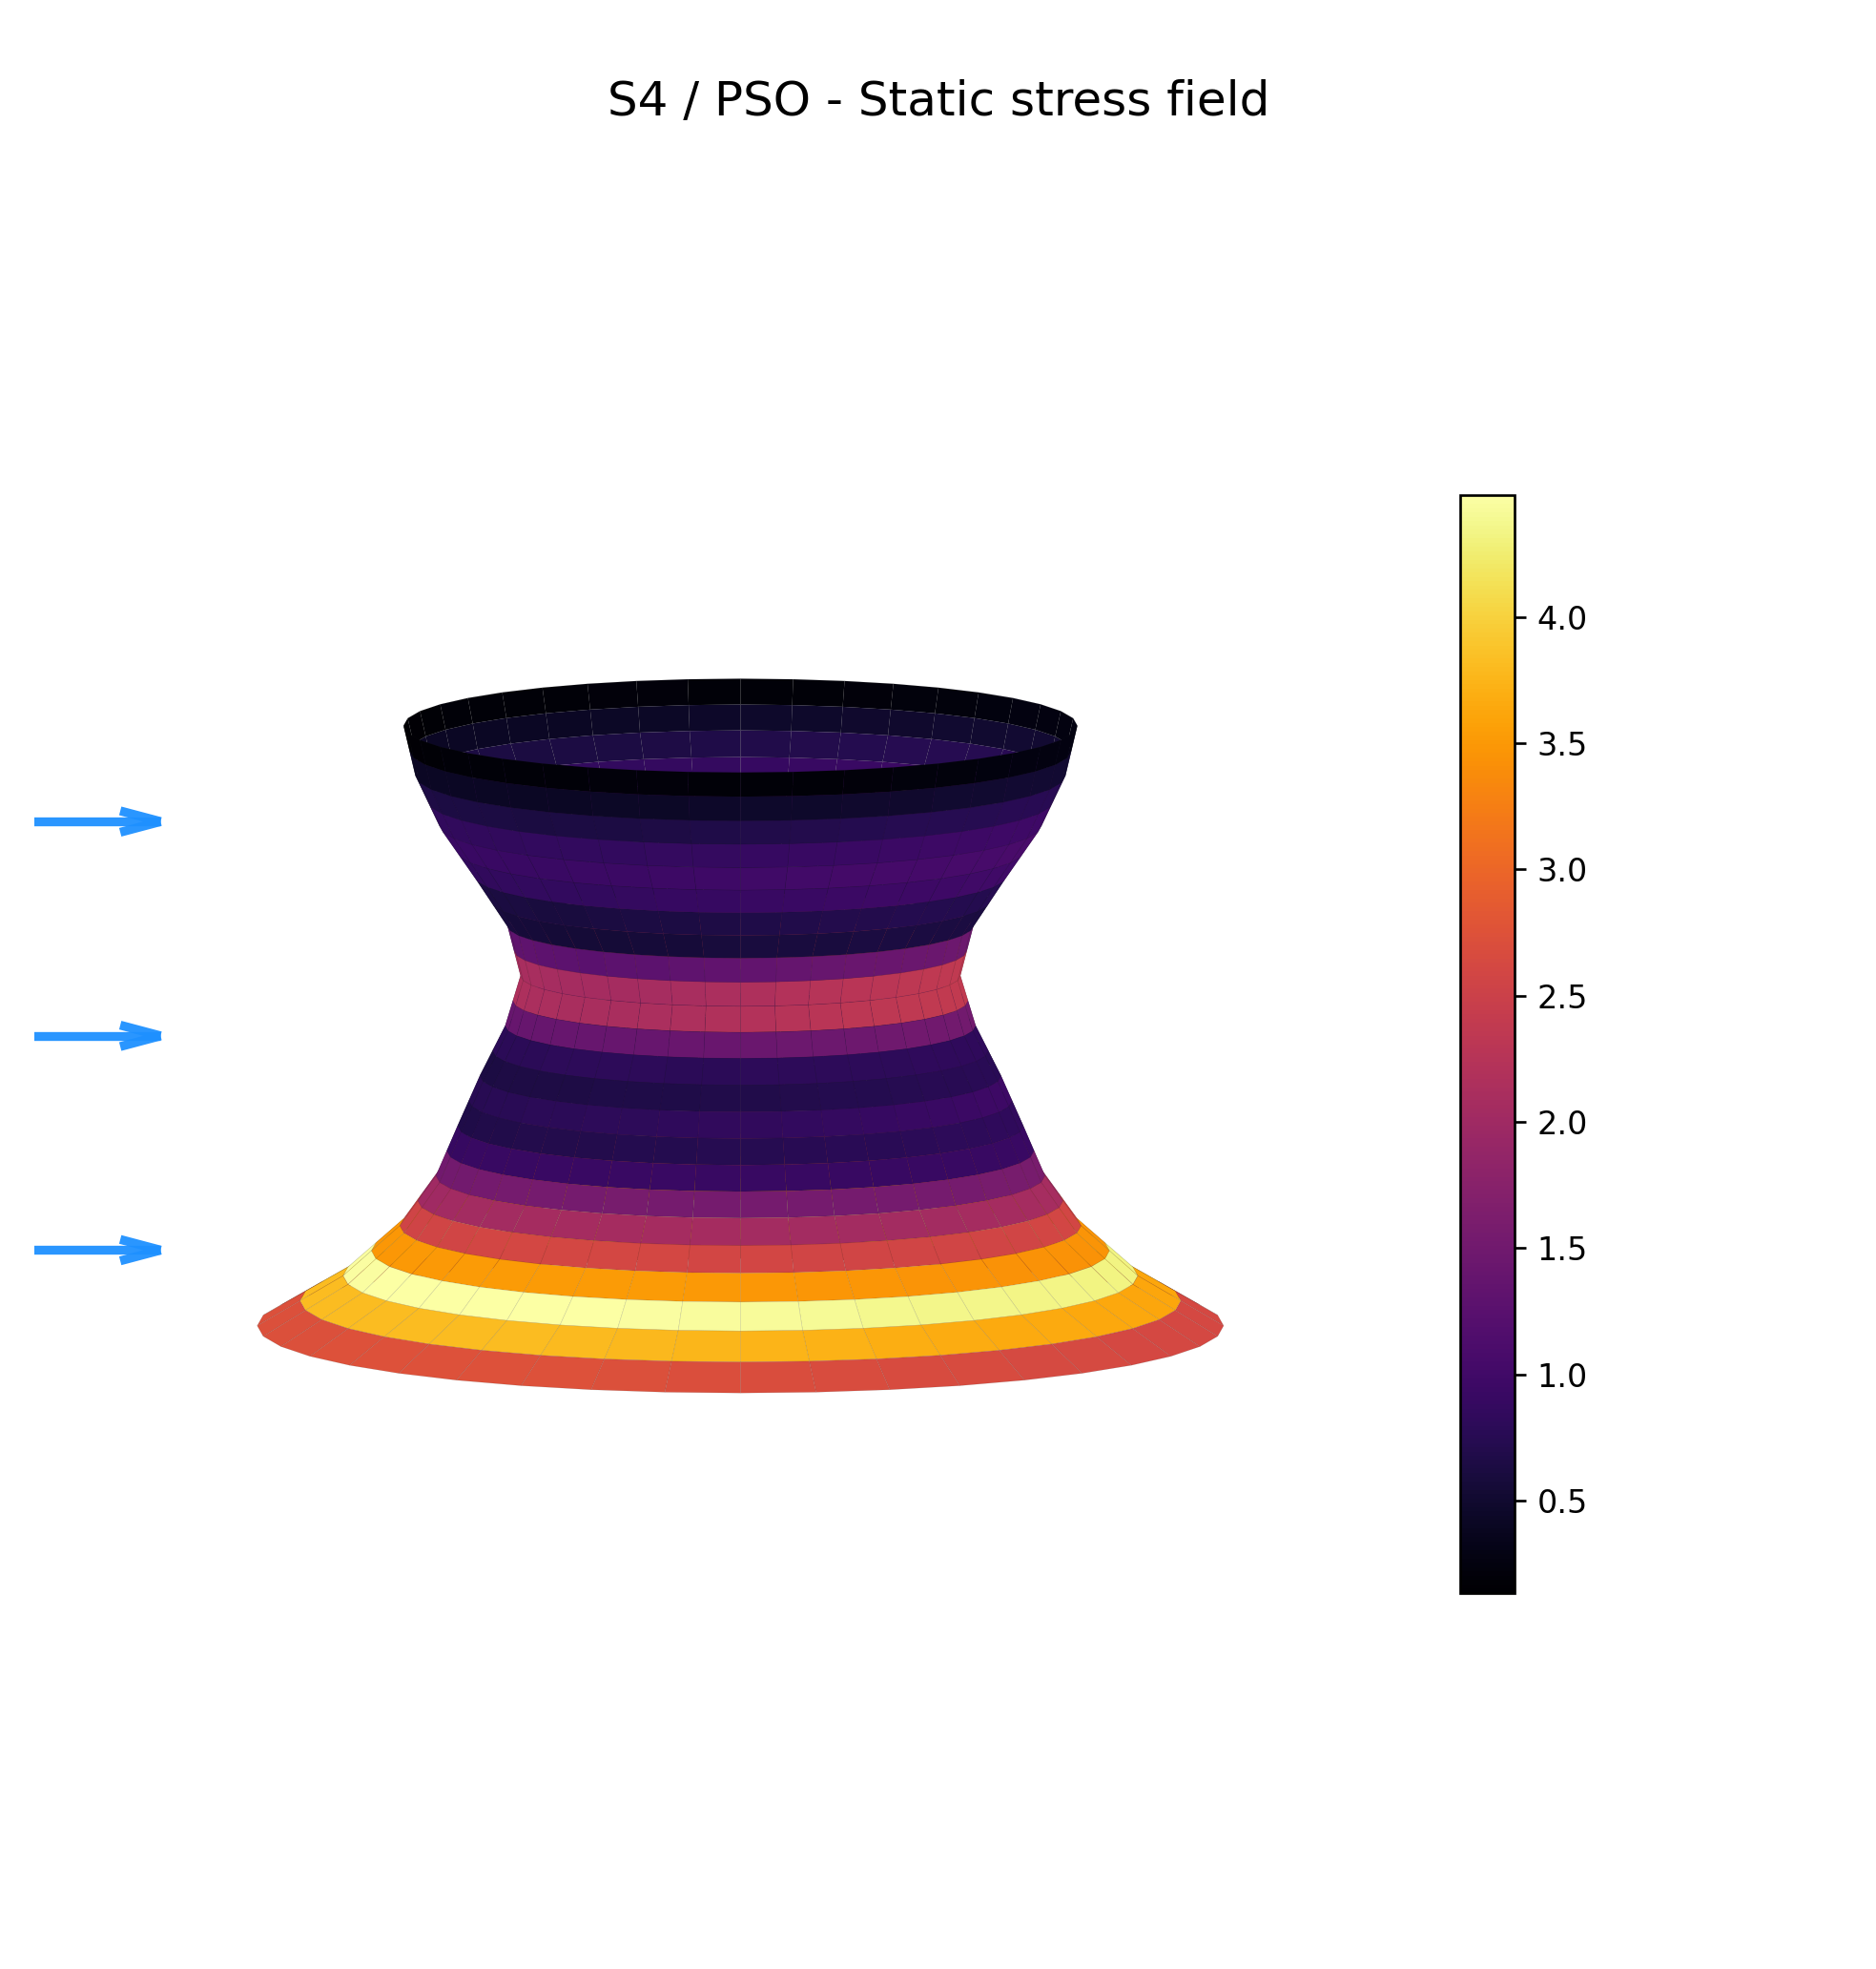
\includegraphics[width=\textwidth]{../results/figures/task7_s4_pso_stress.png}
\caption{S4 / PSO stress}
\end{subfigure}\hfill
\begin{subfigure}{0.32\textwidth}
\centering
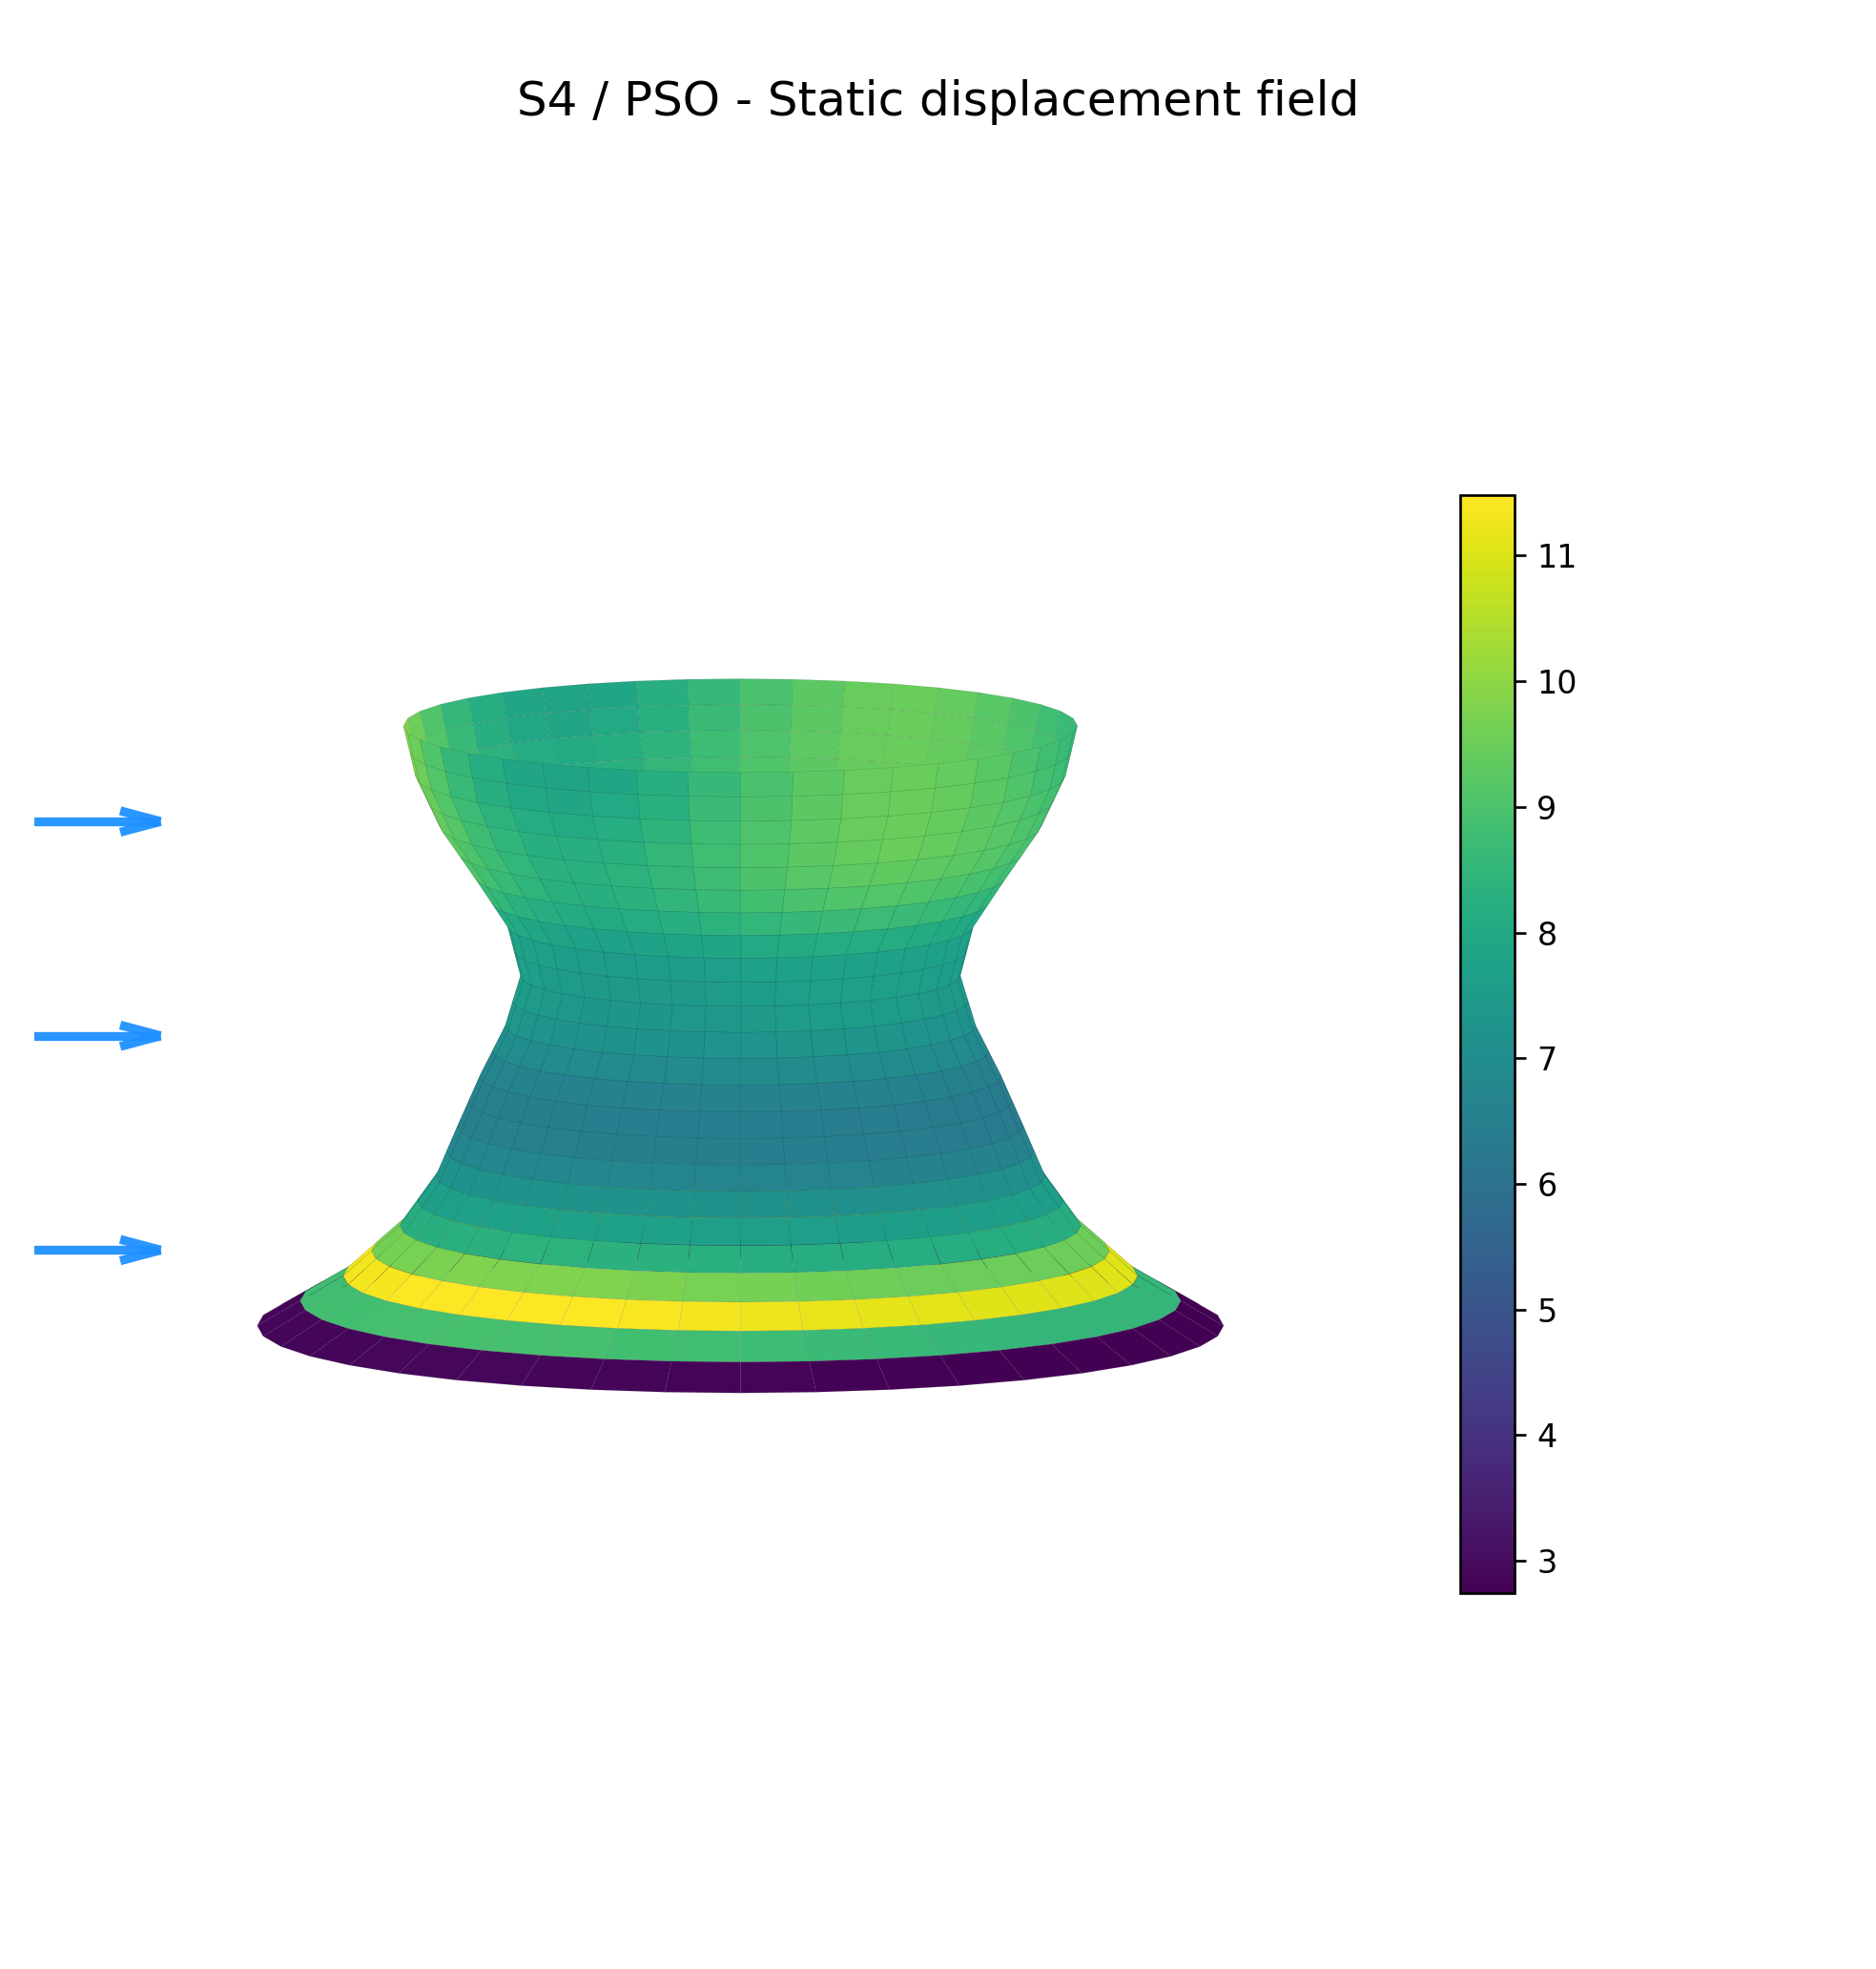
\includegraphics[width=\textwidth]{../results/figures/task7_s4_pso_displacement.png}
\caption{S4 / PSO displacement}
\end{subfigure}\hfill
\begin{subfigure}{0.32\textwidth}
\centering
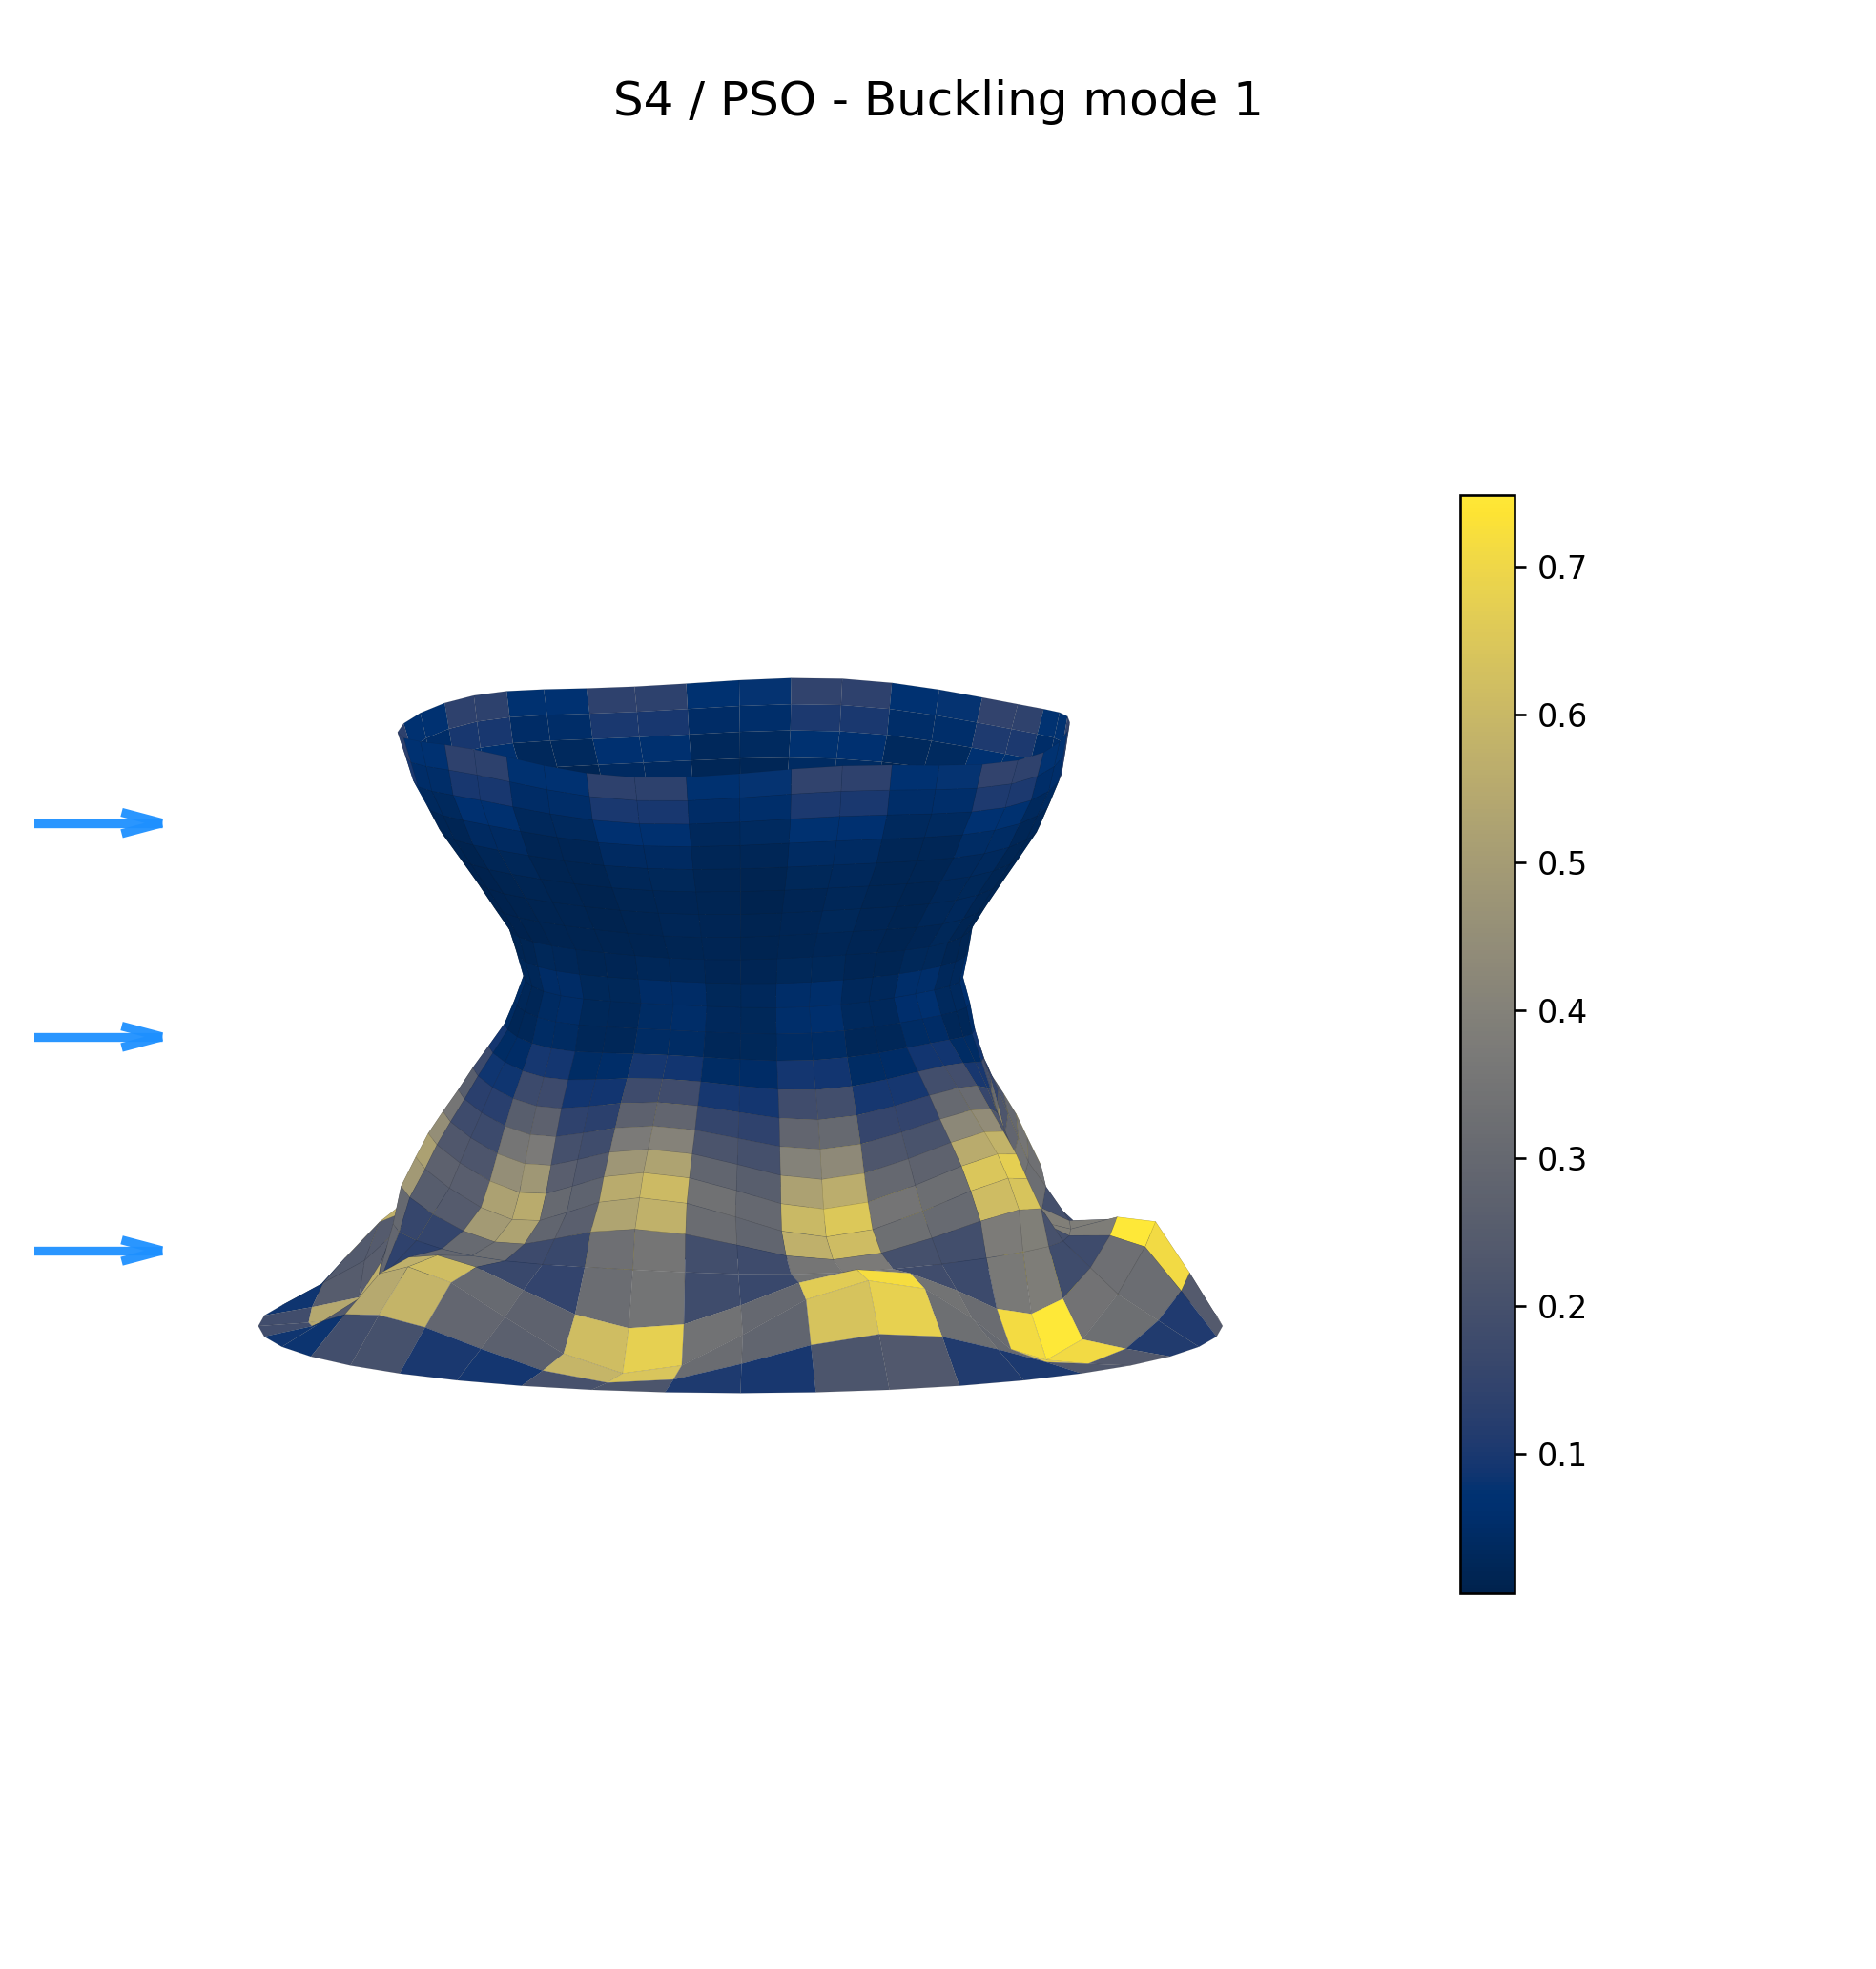
\includegraphics[width=\textwidth]{../results/figures/task7_s4_pso_buckling_mode1.png}
\caption{S4 / PSO buckling}
\end{subfigure}
\caption{Combined visual fields}
\end{figure}


\subsection{S4 / SA}


\begin{figure}[H]
\centering
\begin{subfigure}{0.32\textwidth}
\centering
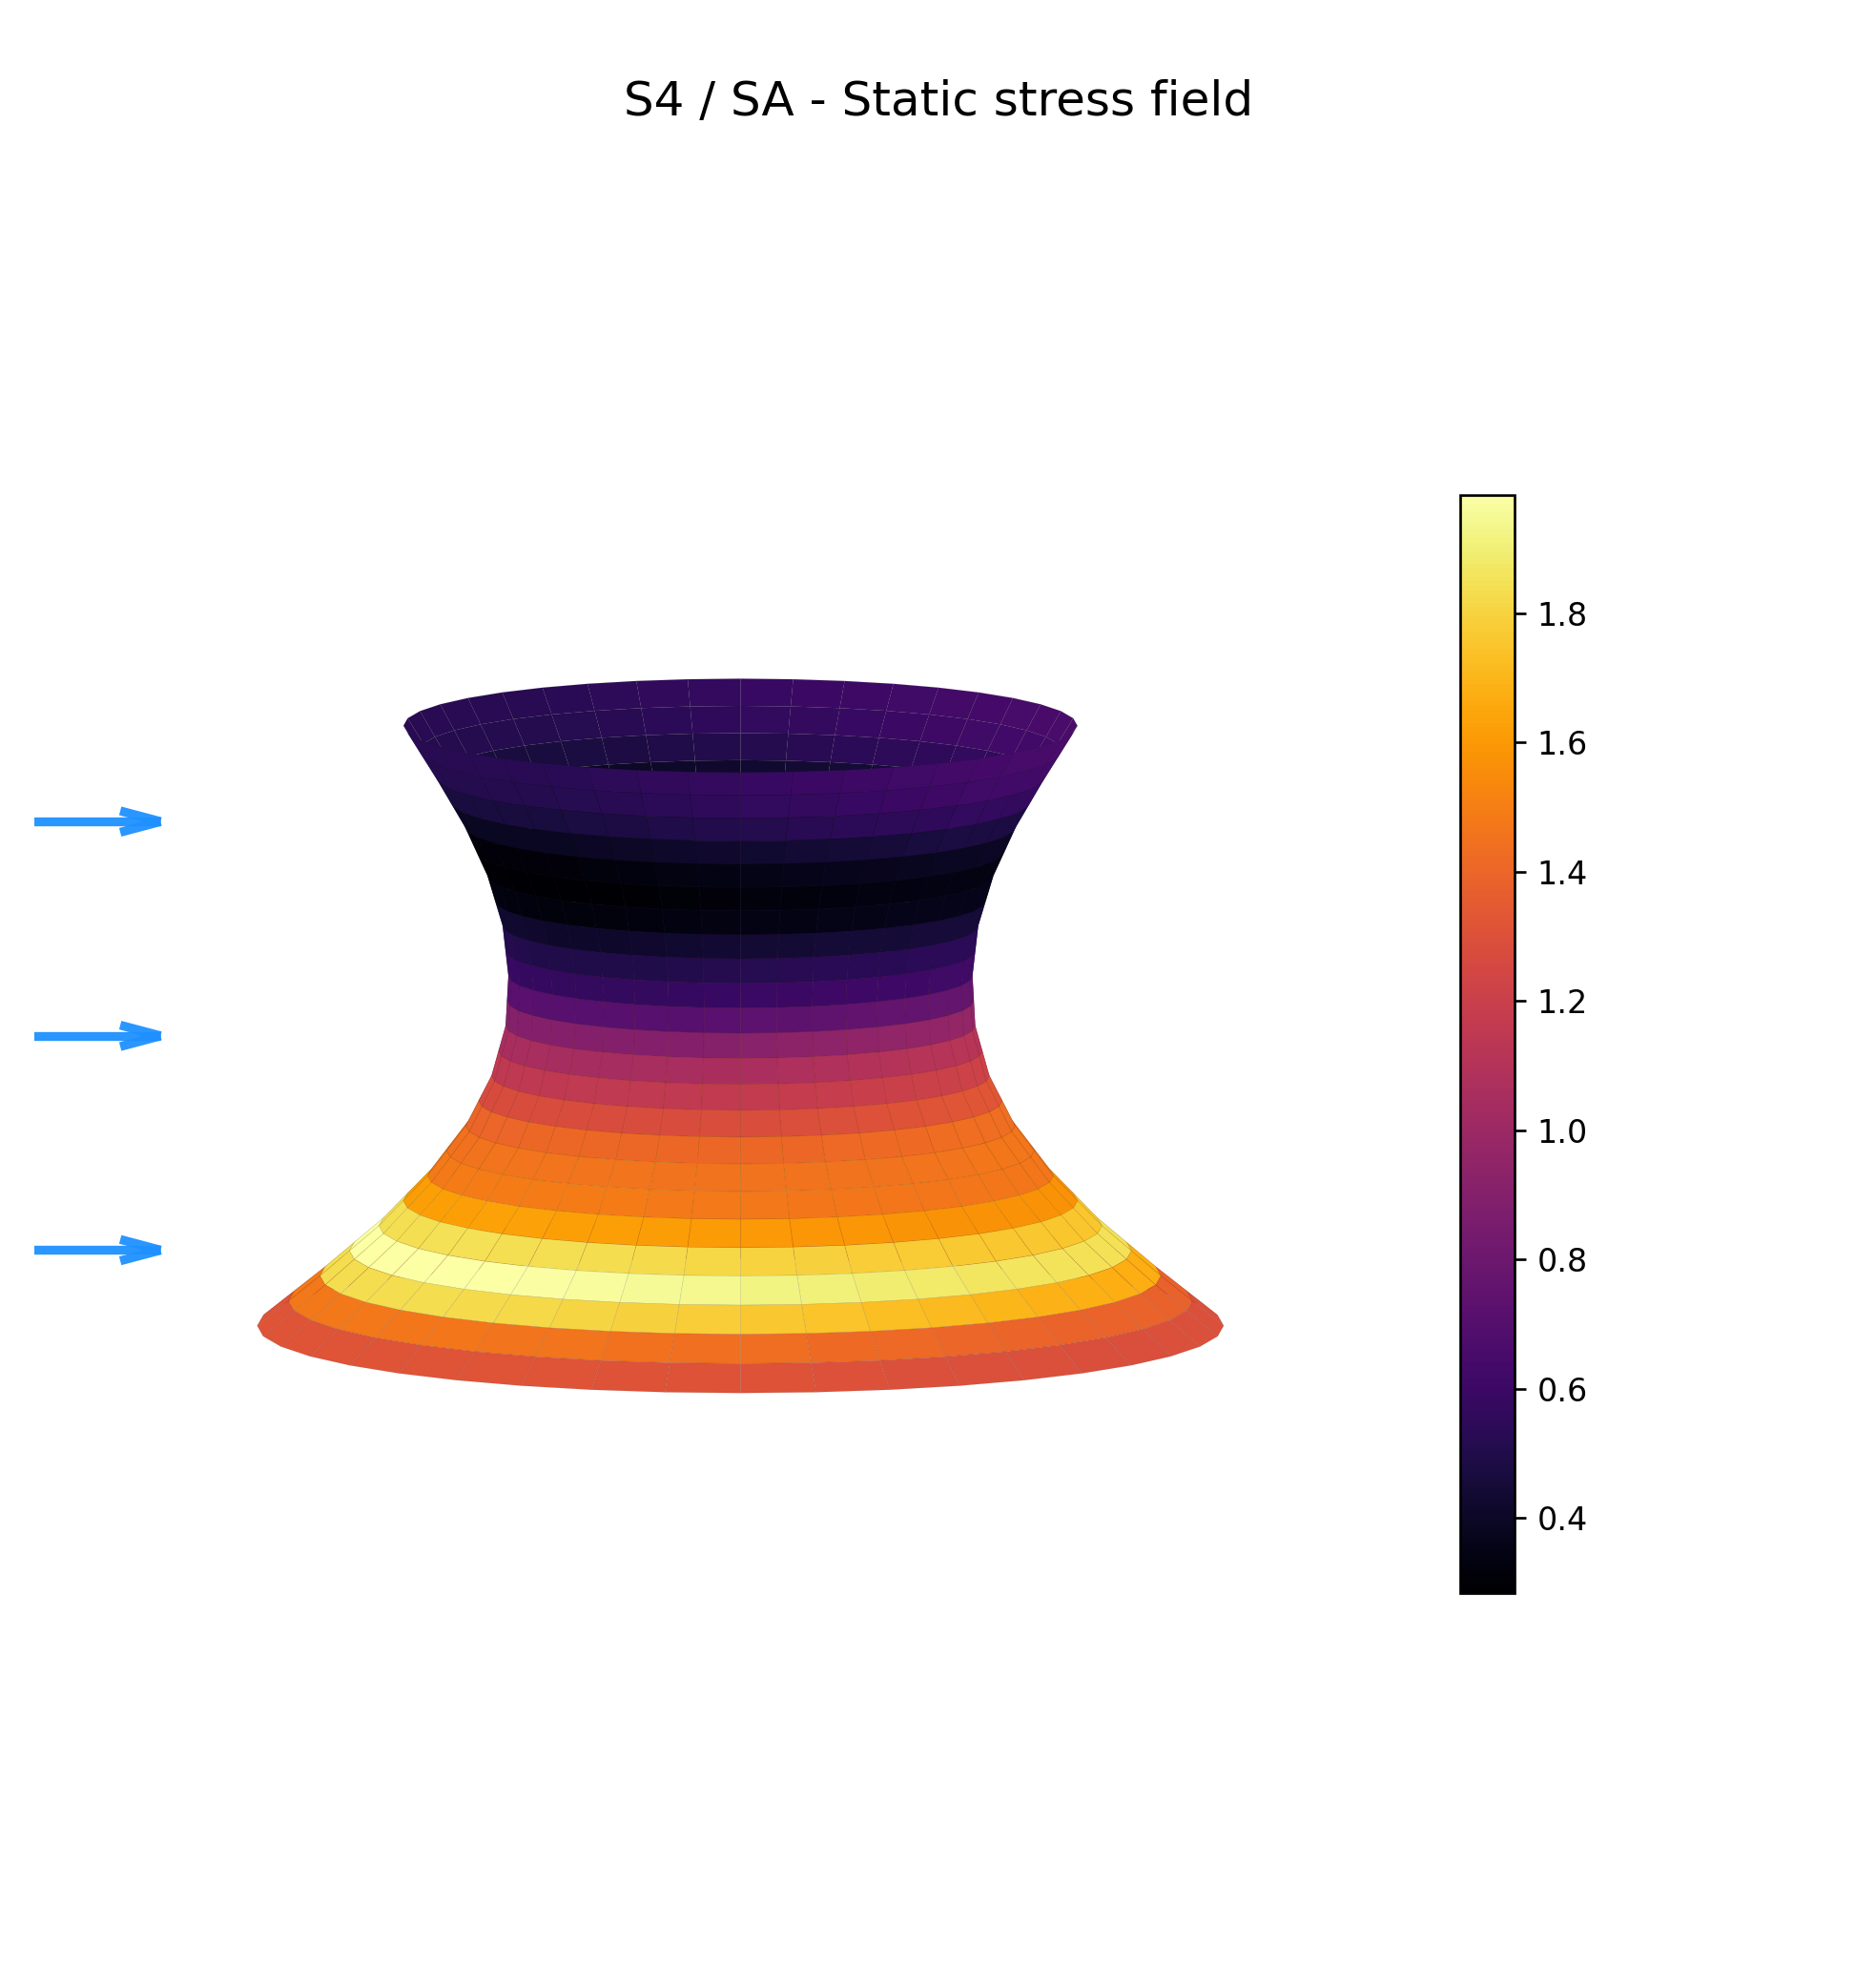
\includegraphics[width=\textwidth]{../results/figures/task7_s4_sa_stress.png}
\caption{S4 / SA stress}
\end{subfigure}\hfill
\begin{subfigure}{0.32\textwidth}
\centering
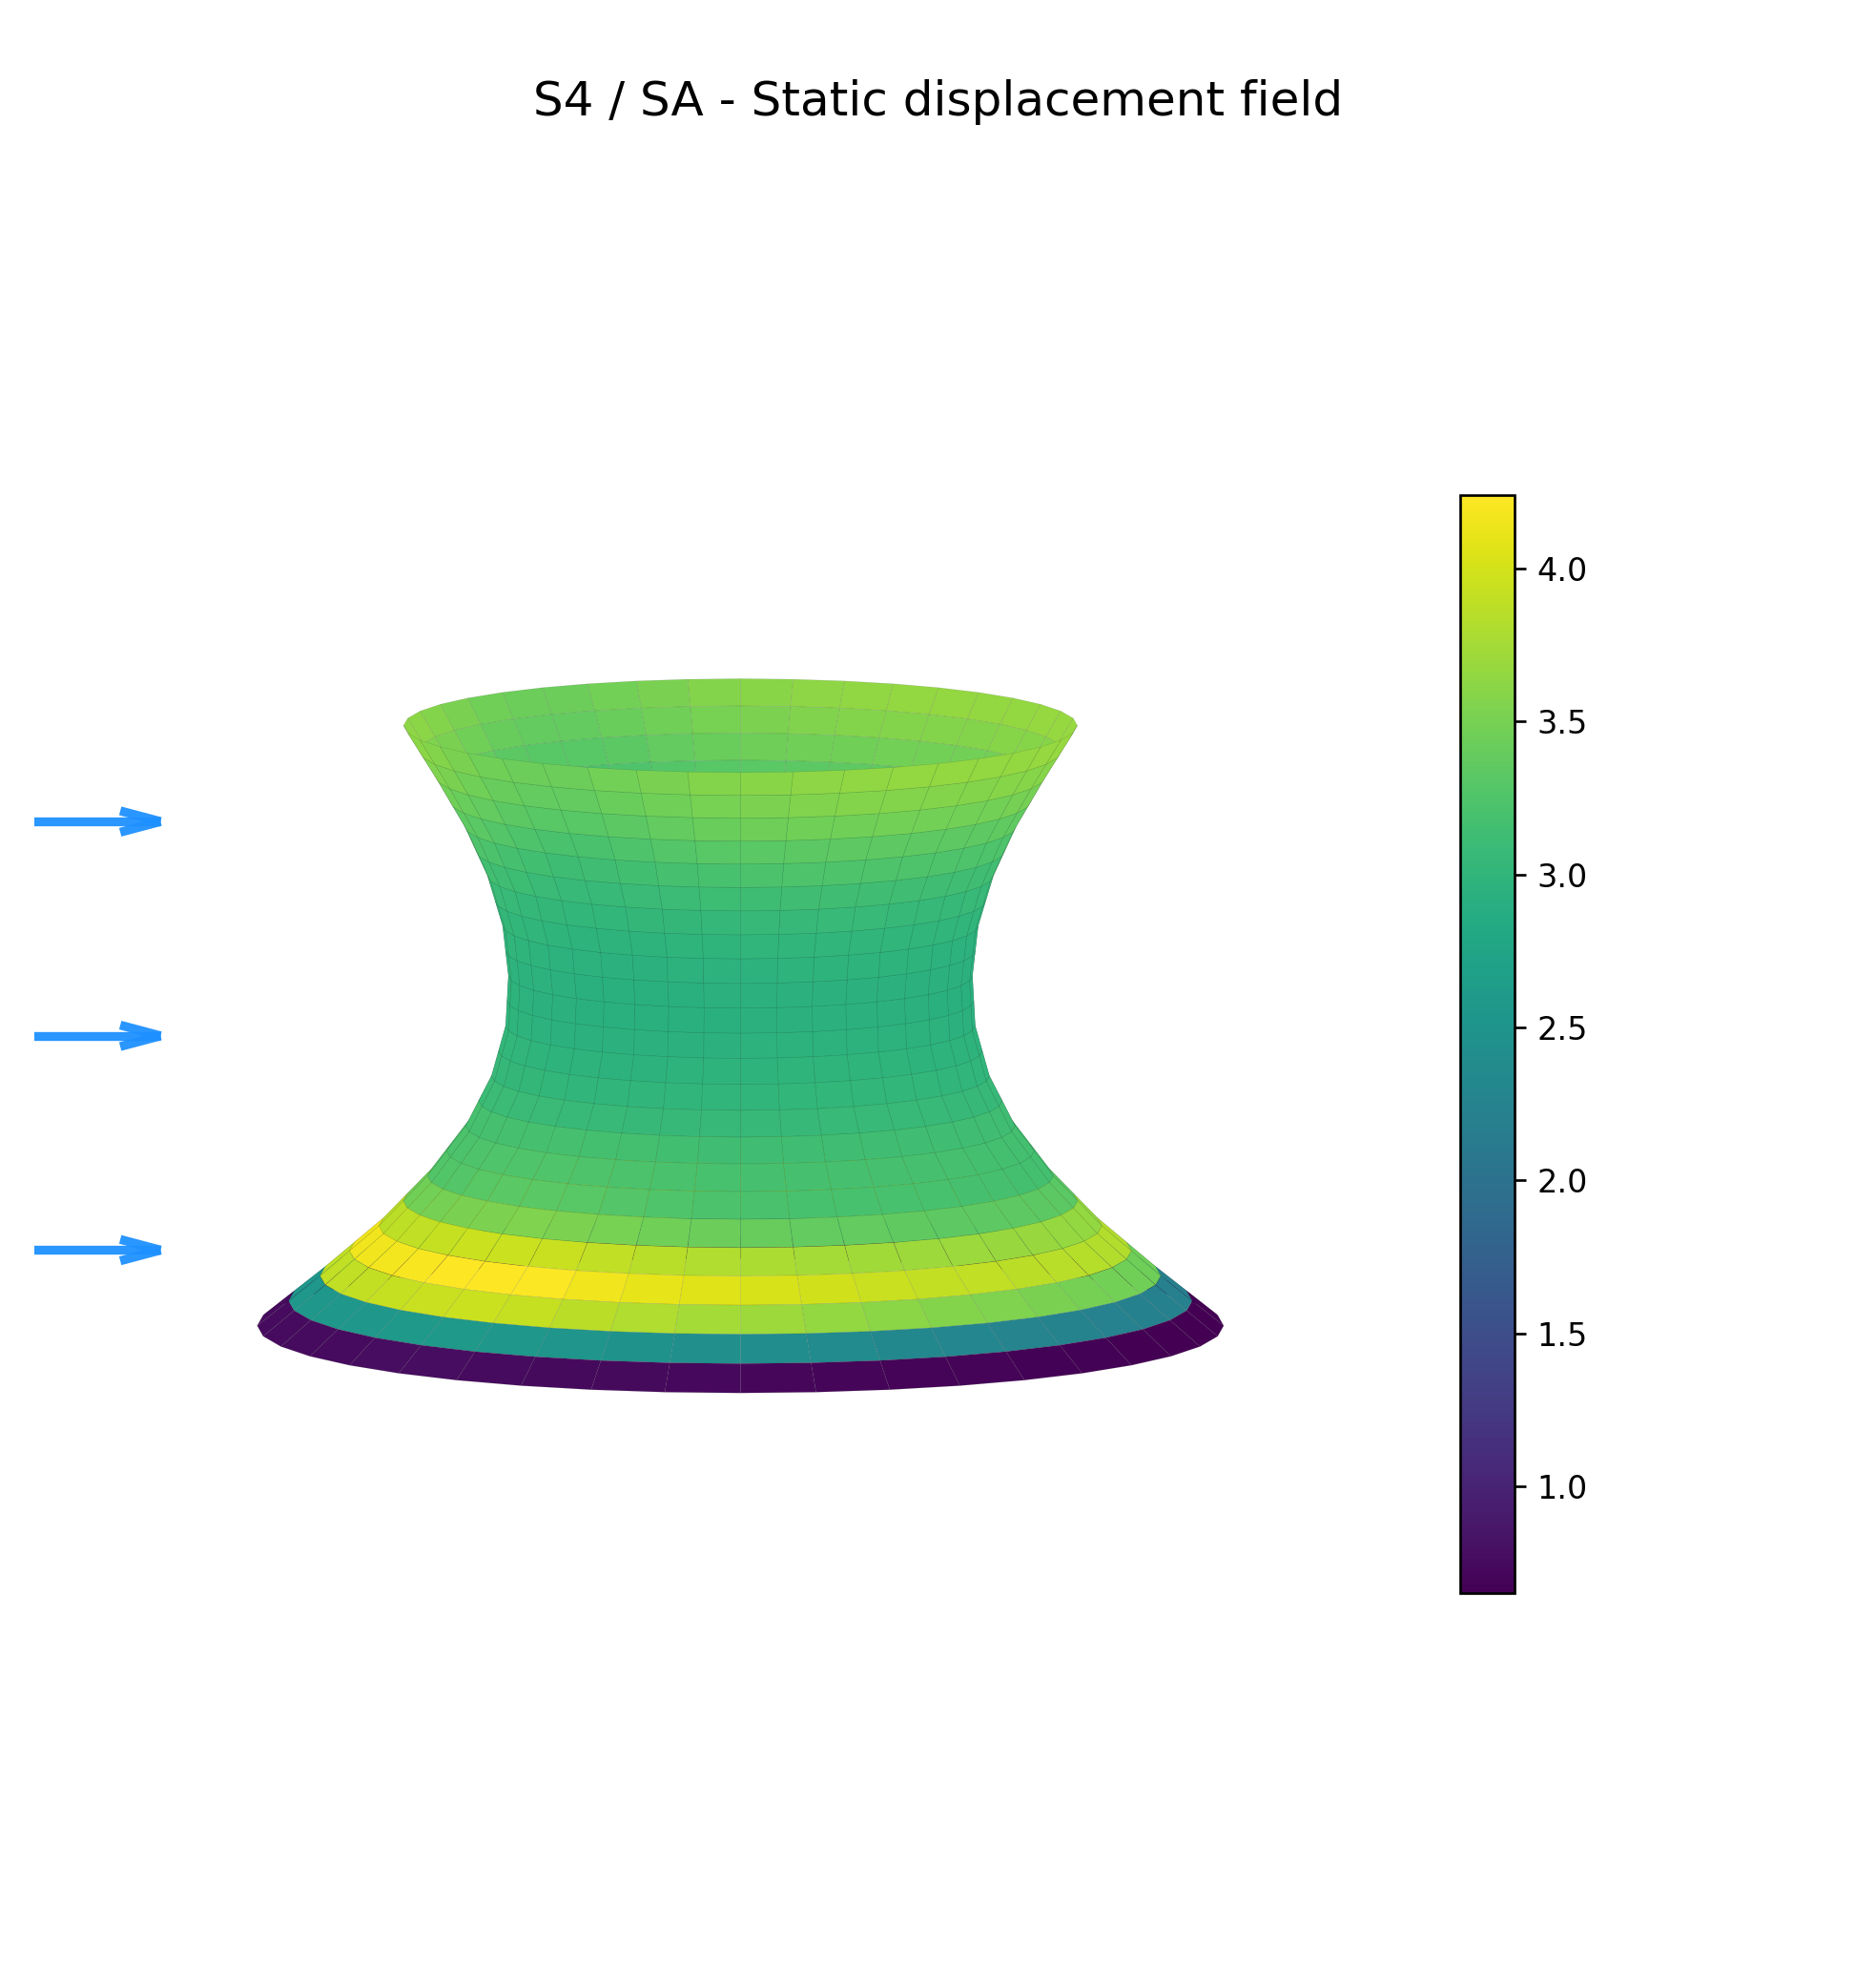
\includegraphics[width=\textwidth]{../results/figures/task7_s4_sa_displacement.png}
\caption{S4 / SA displacement}
\end{subfigure}\hfill
\begin{subfigure}{0.32\textwidth}
\centering
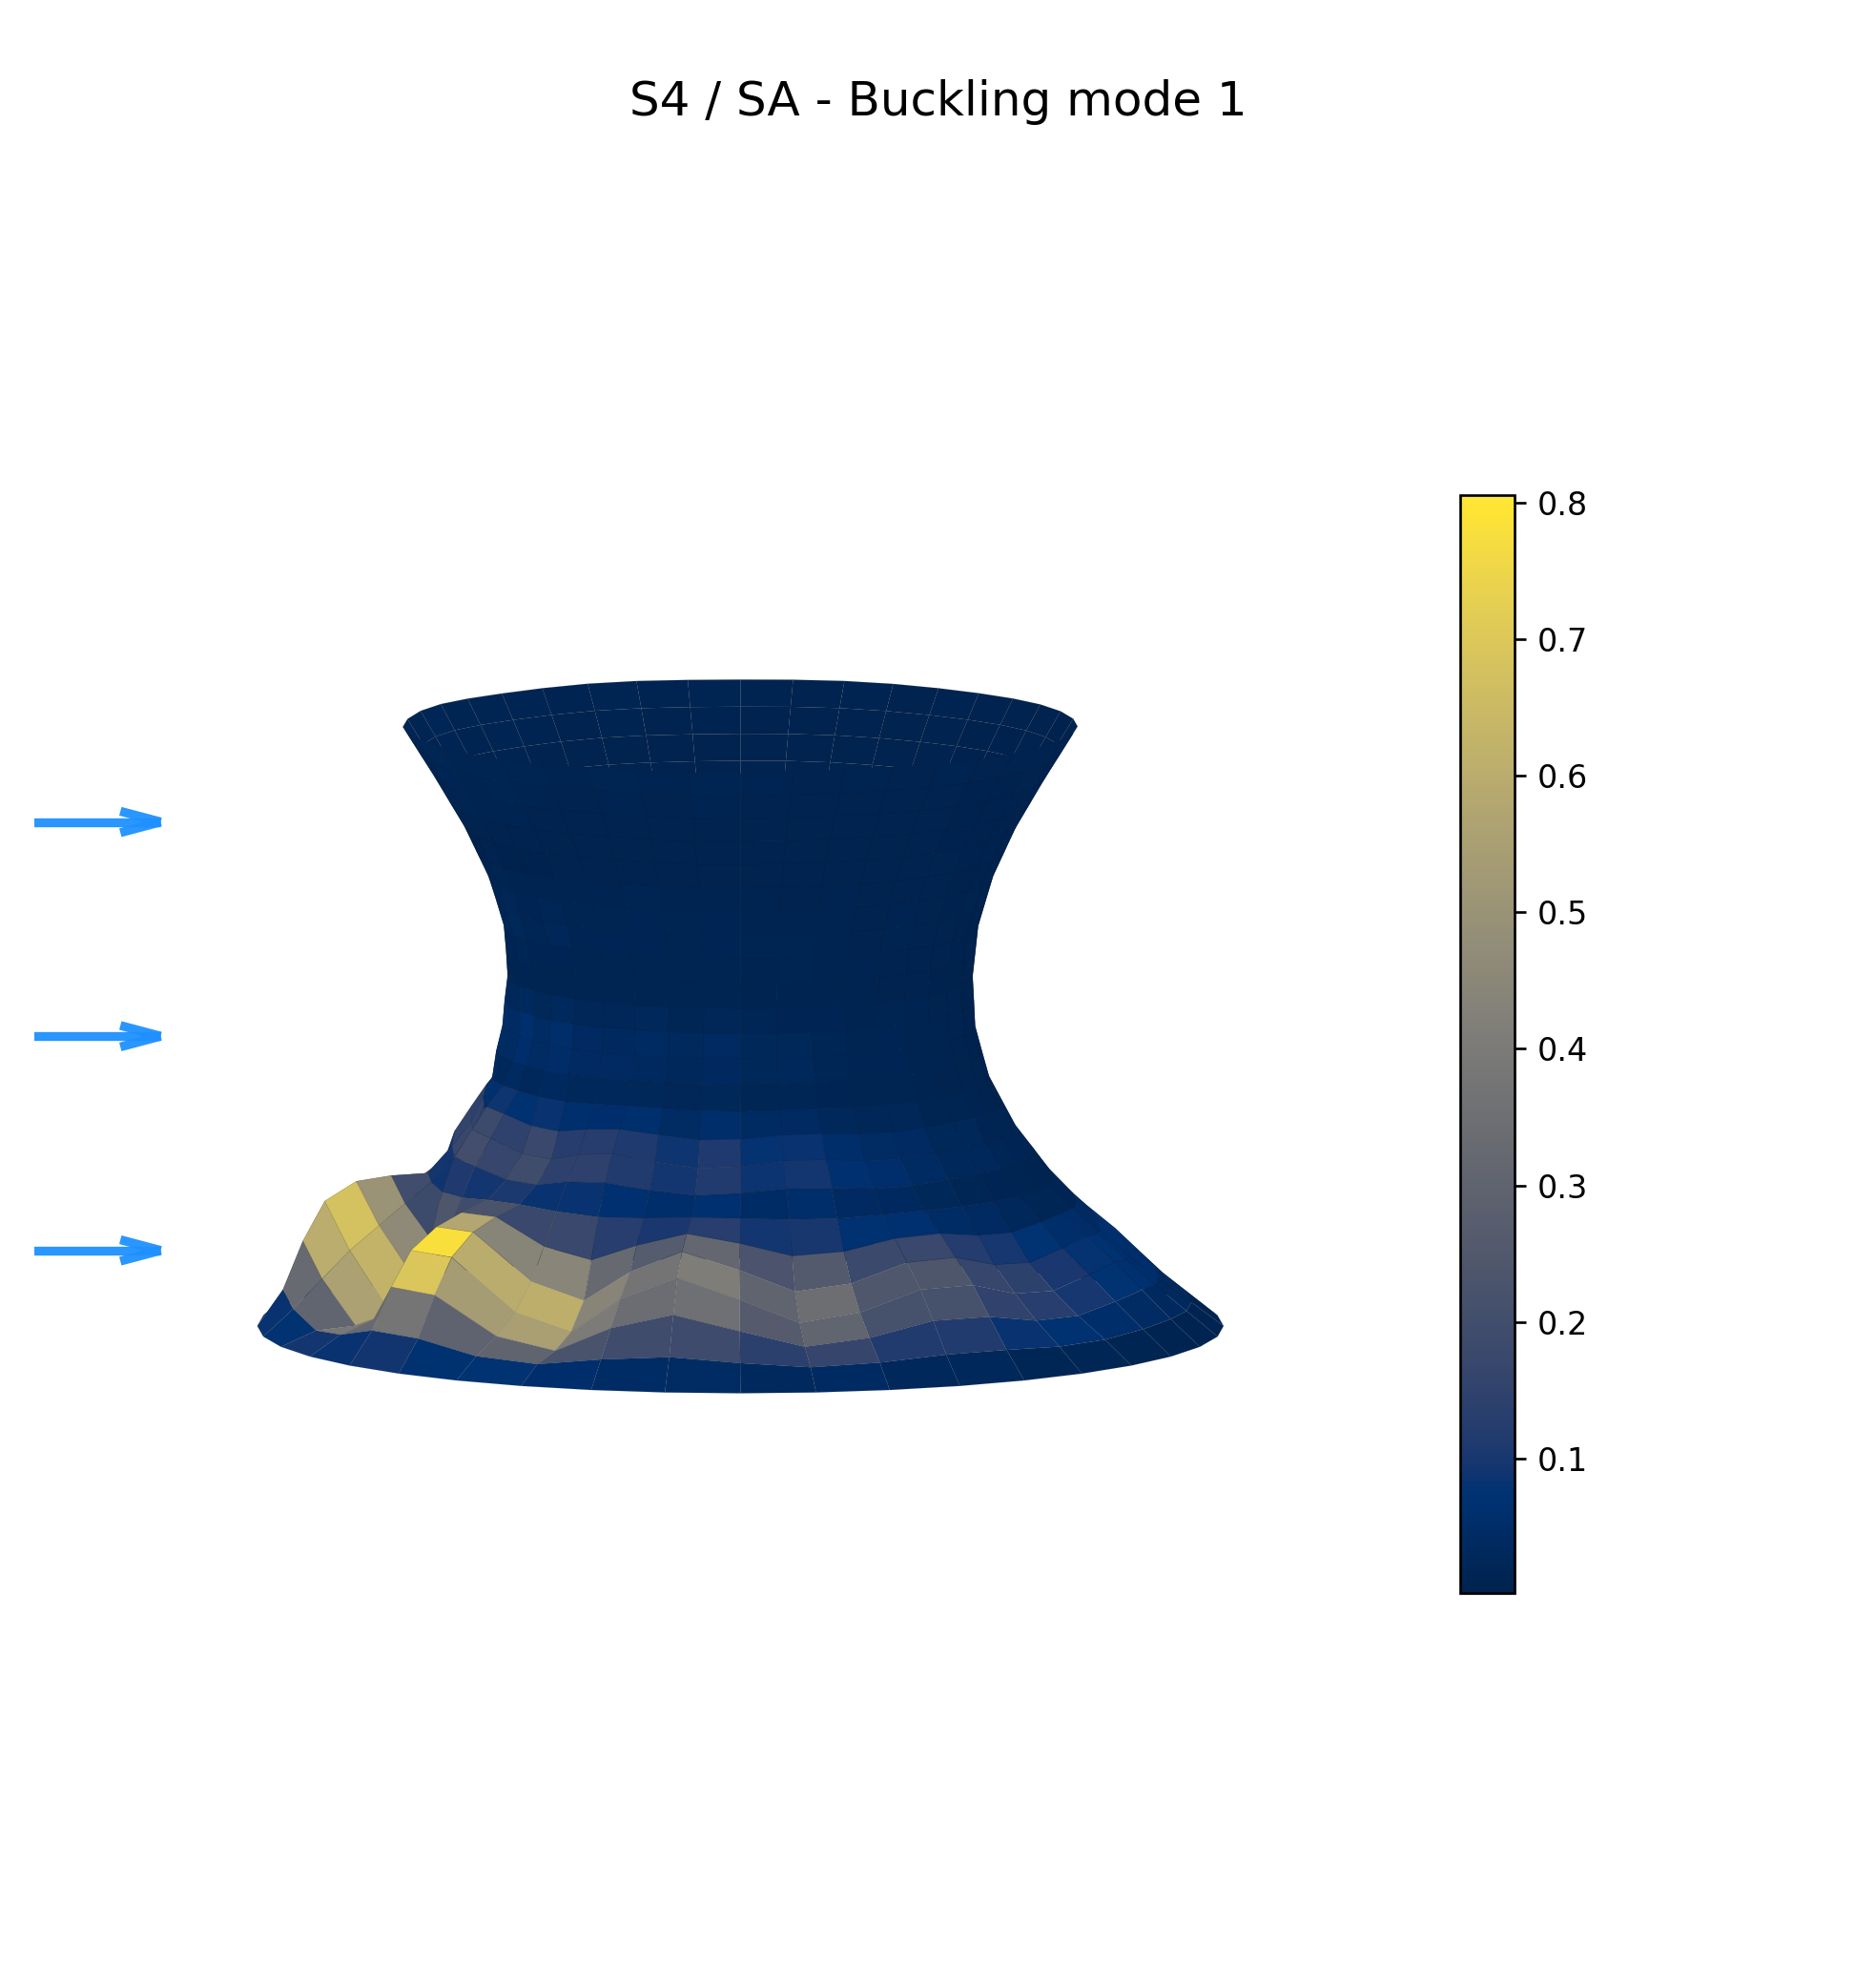
\includegraphics[width=\textwidth]{../results/figures/task7_s4_sa_buckling_mode1.png}
\caption{S4 / SA buckling}
\end{subfigure}
\caption{Combined visual fields}
\end{figure}


\section{Scenario S5}


\subsection{S5 / BFGS}


\begin{figure}[H]
\centering
\begin{subfigure}{0.32\textwidth}
\centering
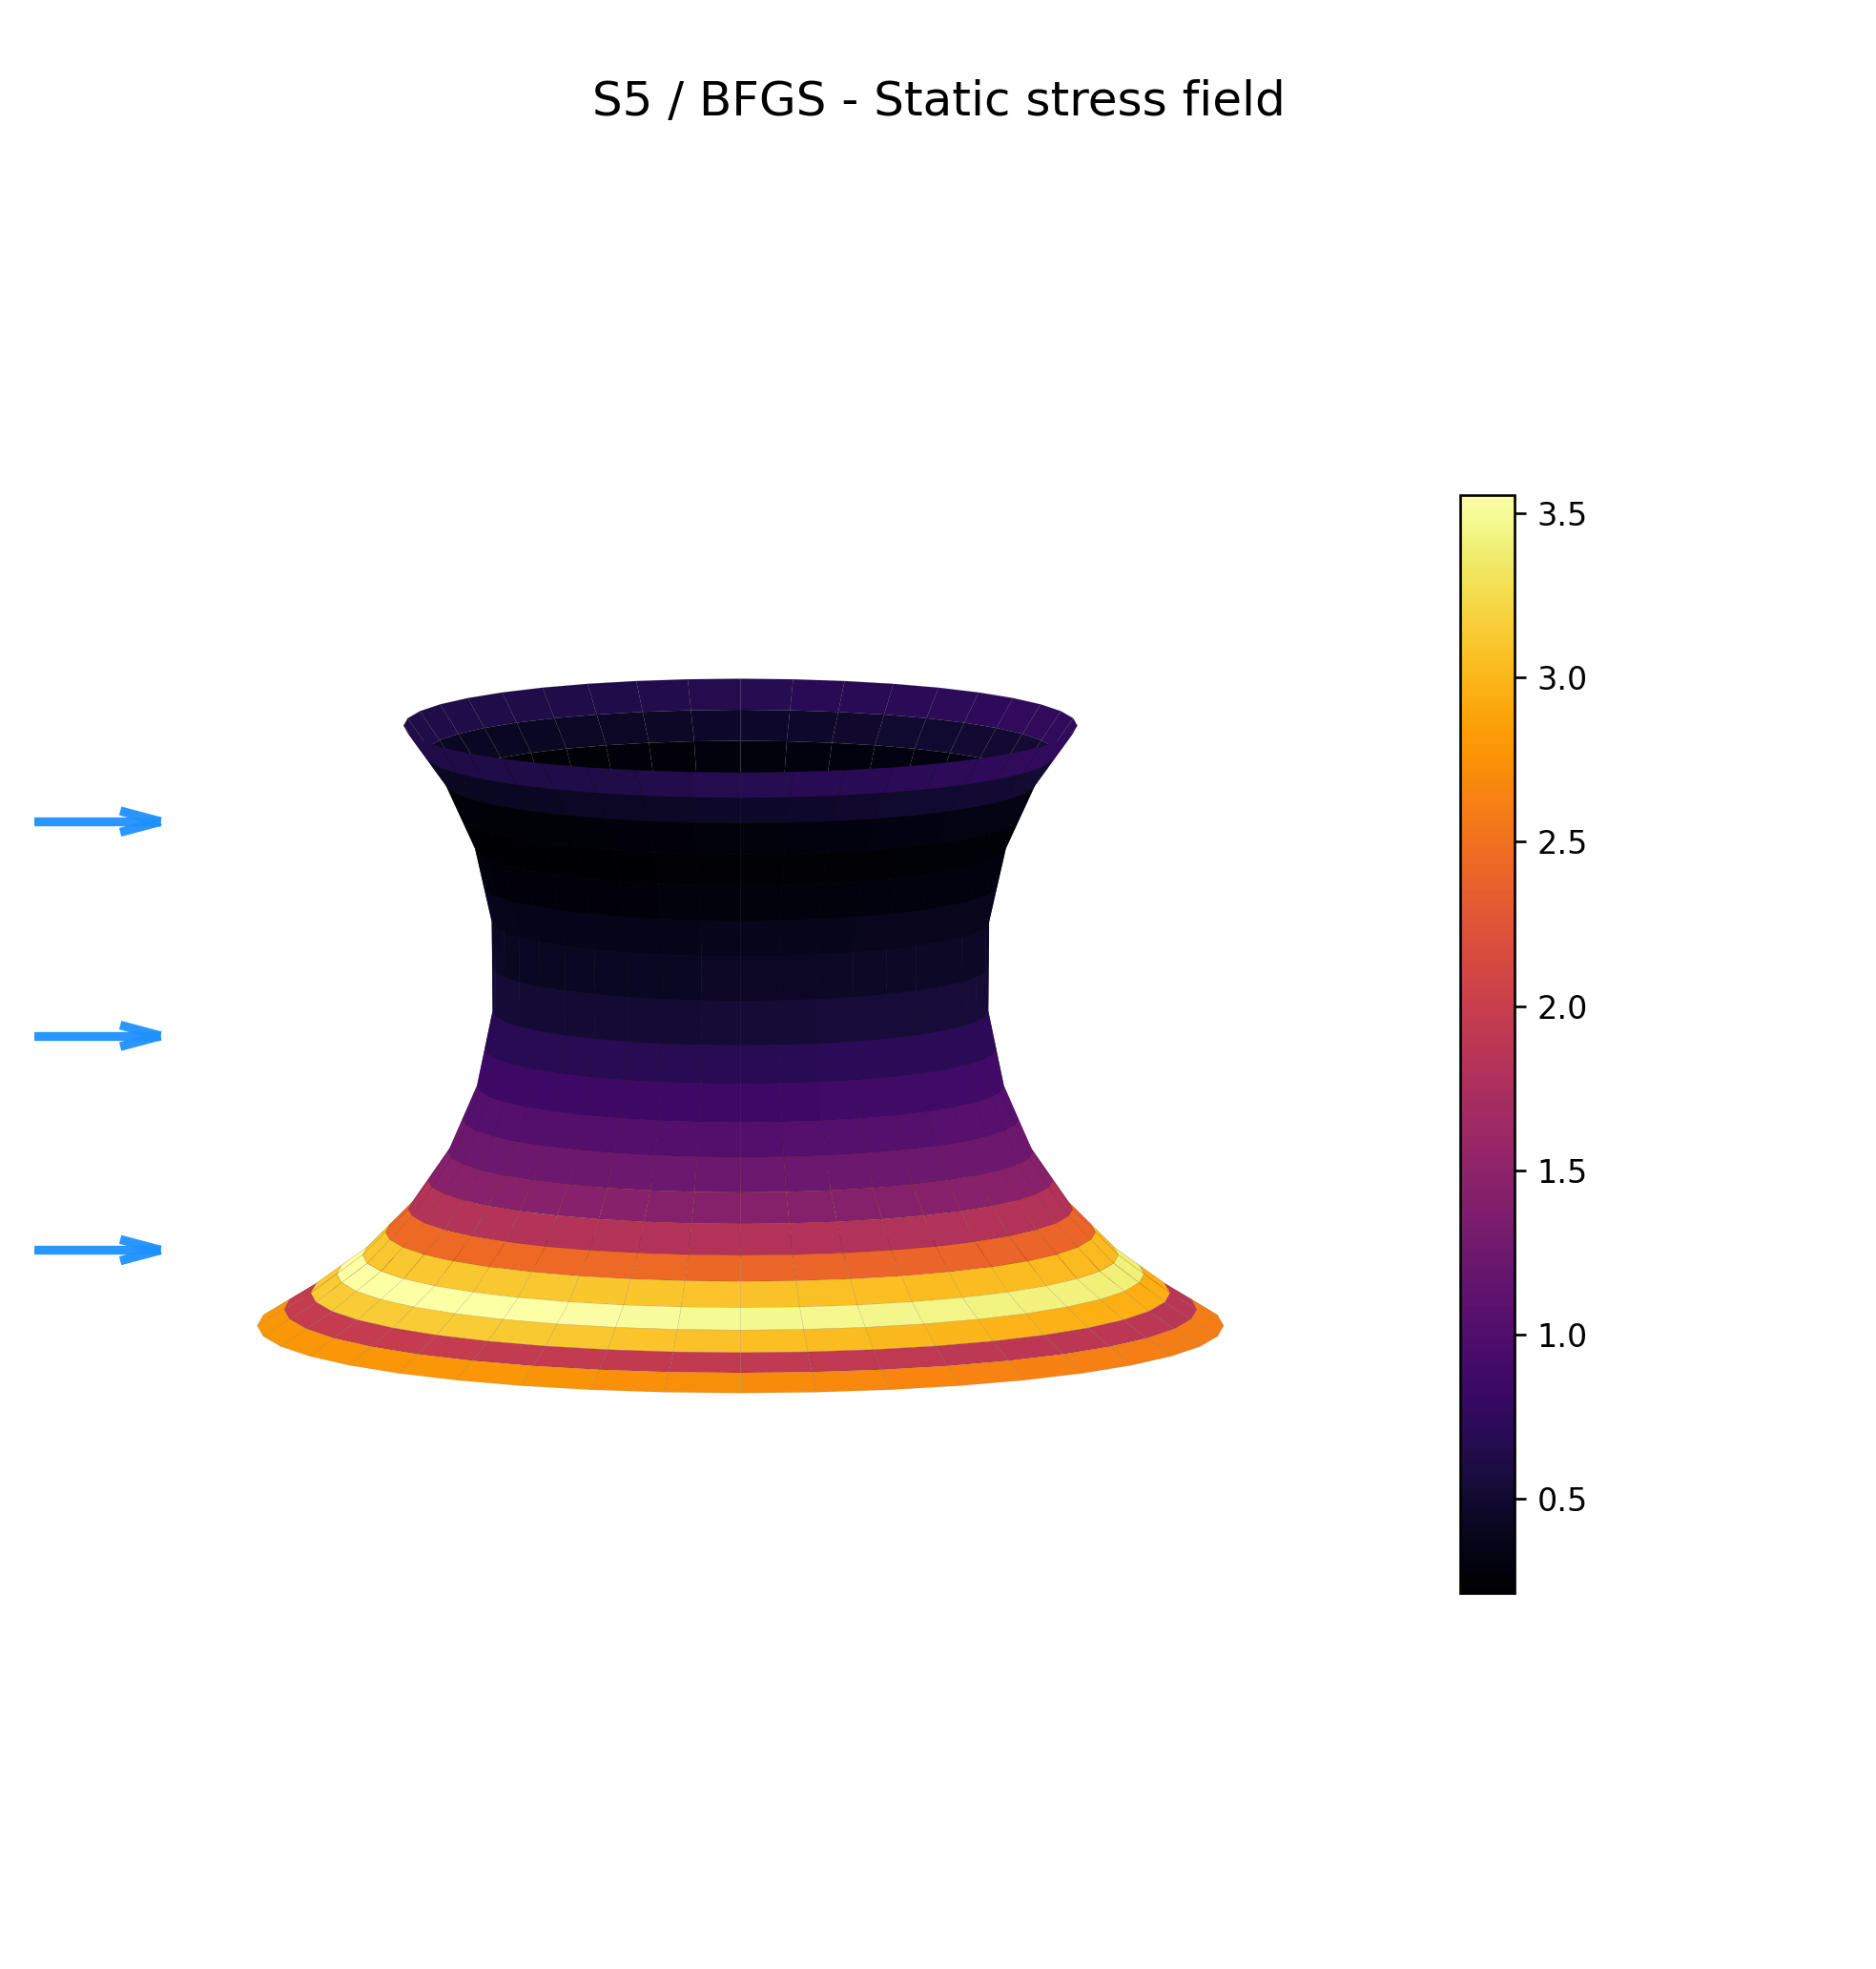
\includegraphics[width=\textwidth]{../results/figures/task7_s5_bfgs_stress.png}
\caption{S5 / BFGS stress}
\end{subfigure}\hfill
\begin{subfigure}{0.32\textwidth}
\centering
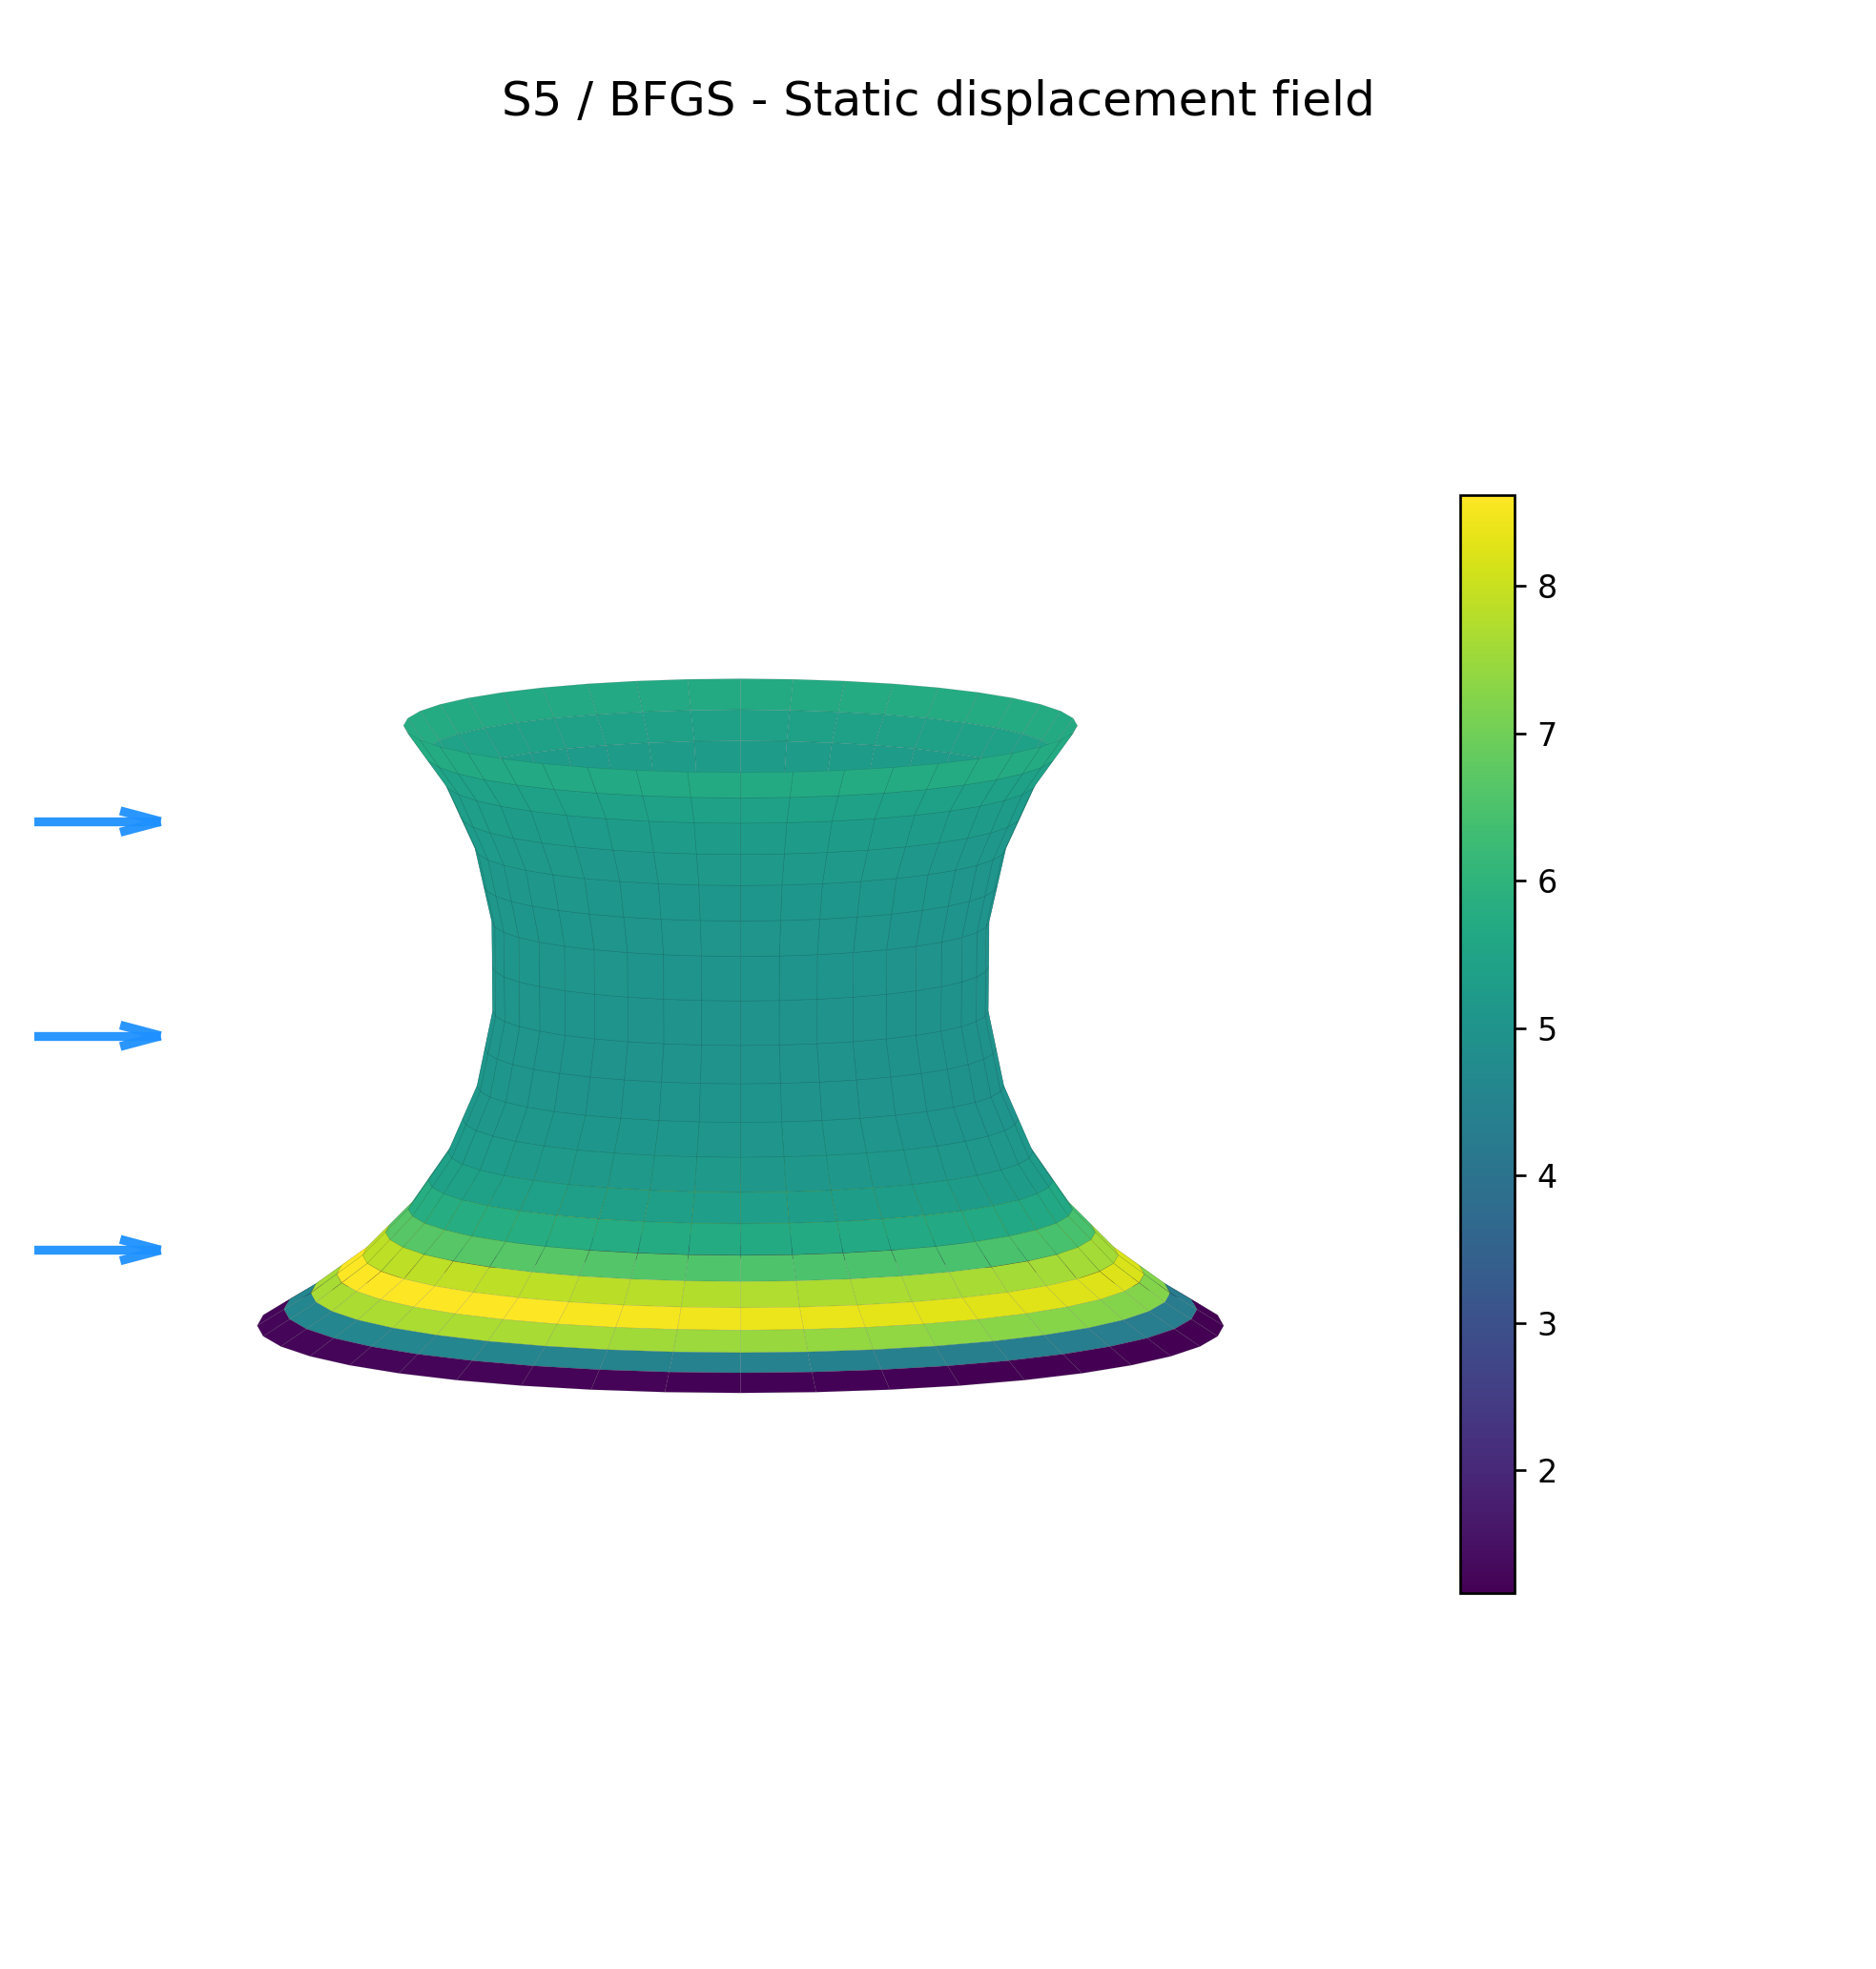
\includegraphics[width=\textwidth]{../results/figures/task7_s5_bfgs_displacement.png}
\caption{S5 / BFGS displacement}
\end{subfigure}\hfill
\begin{subfigure}{0.32\textwidth}
\centering
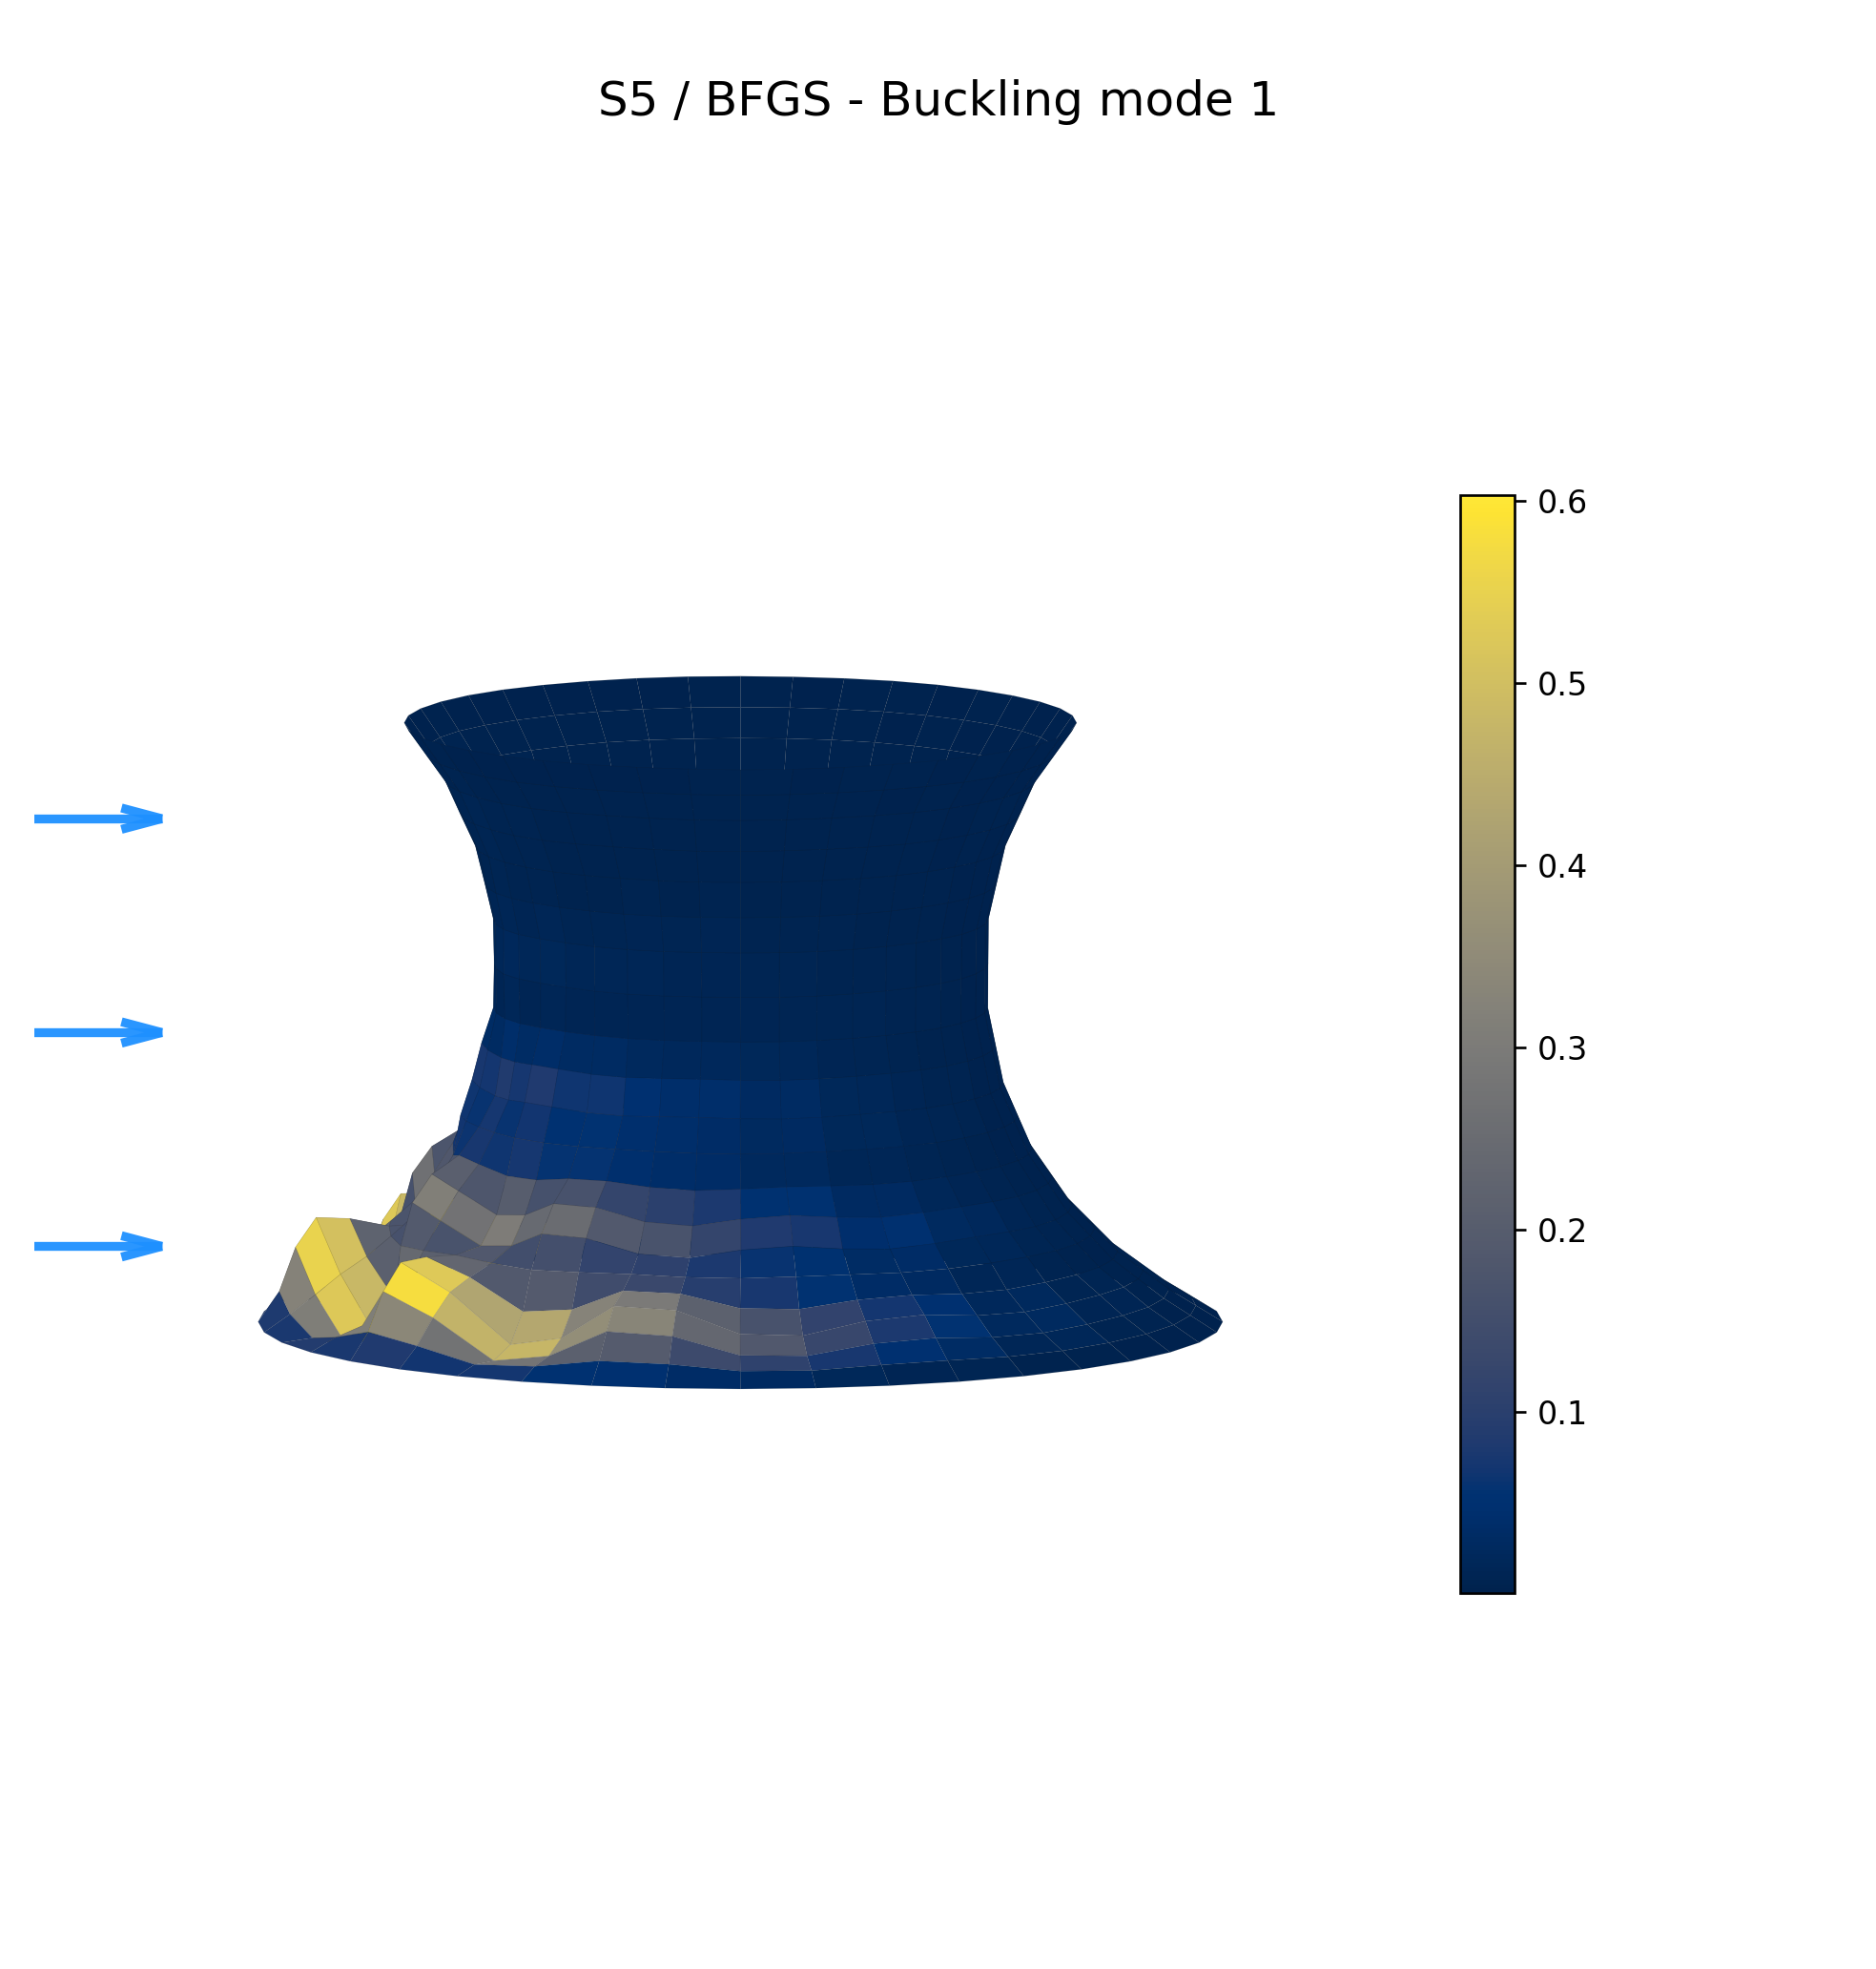
\includegraphics[width=\textwidth]{../results/figures/task7_s5_bfgs_buckling_mode1.png}
\caption{S5 / BFGS buckling}
\end{subfigure}
\caption{Combined visual fields}
\end{figure}


\subsection{S5 / PSO}


\begin{figure}[H]
\centering
\begin{subfigure}{0.32\textwidth}
\centering
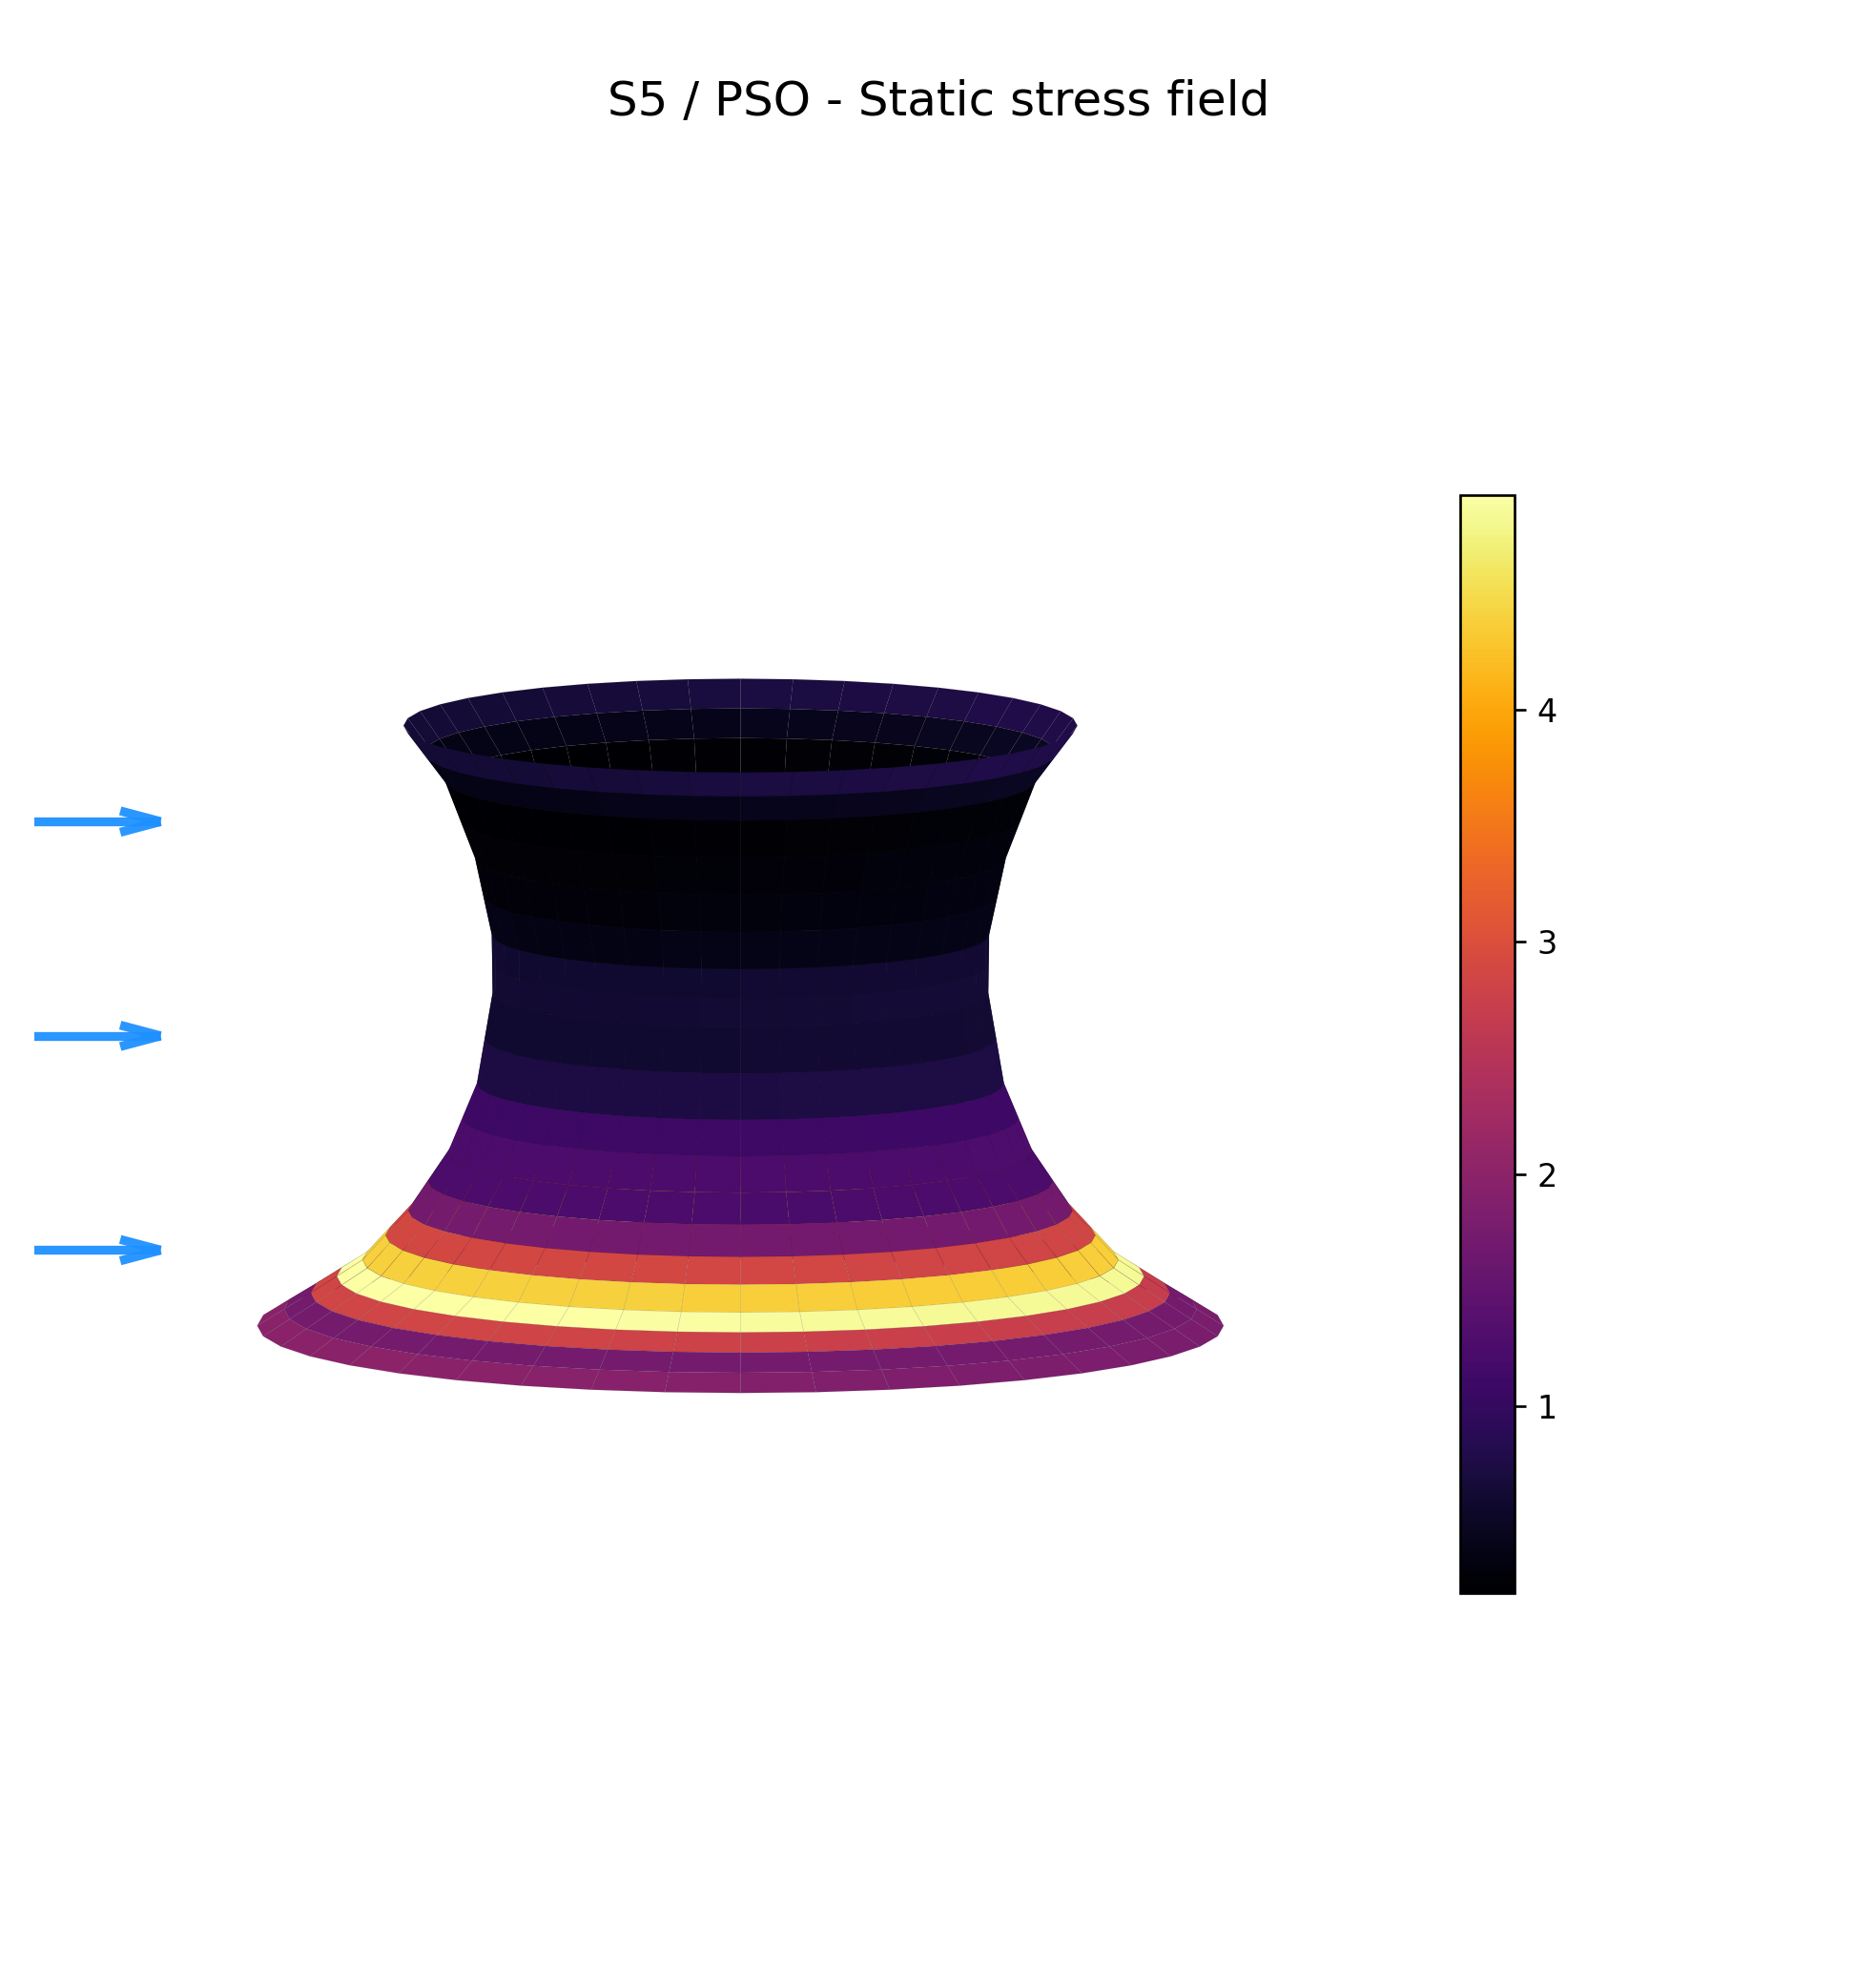
\includegraphics[width=\textwidth]{../results/figures/task7_s5_pso_stress.png}
\caption{S5 / PSO stress}
\end{subfigure}\hfill
\begin{subfigure}{0.32\textwidth}
\centering
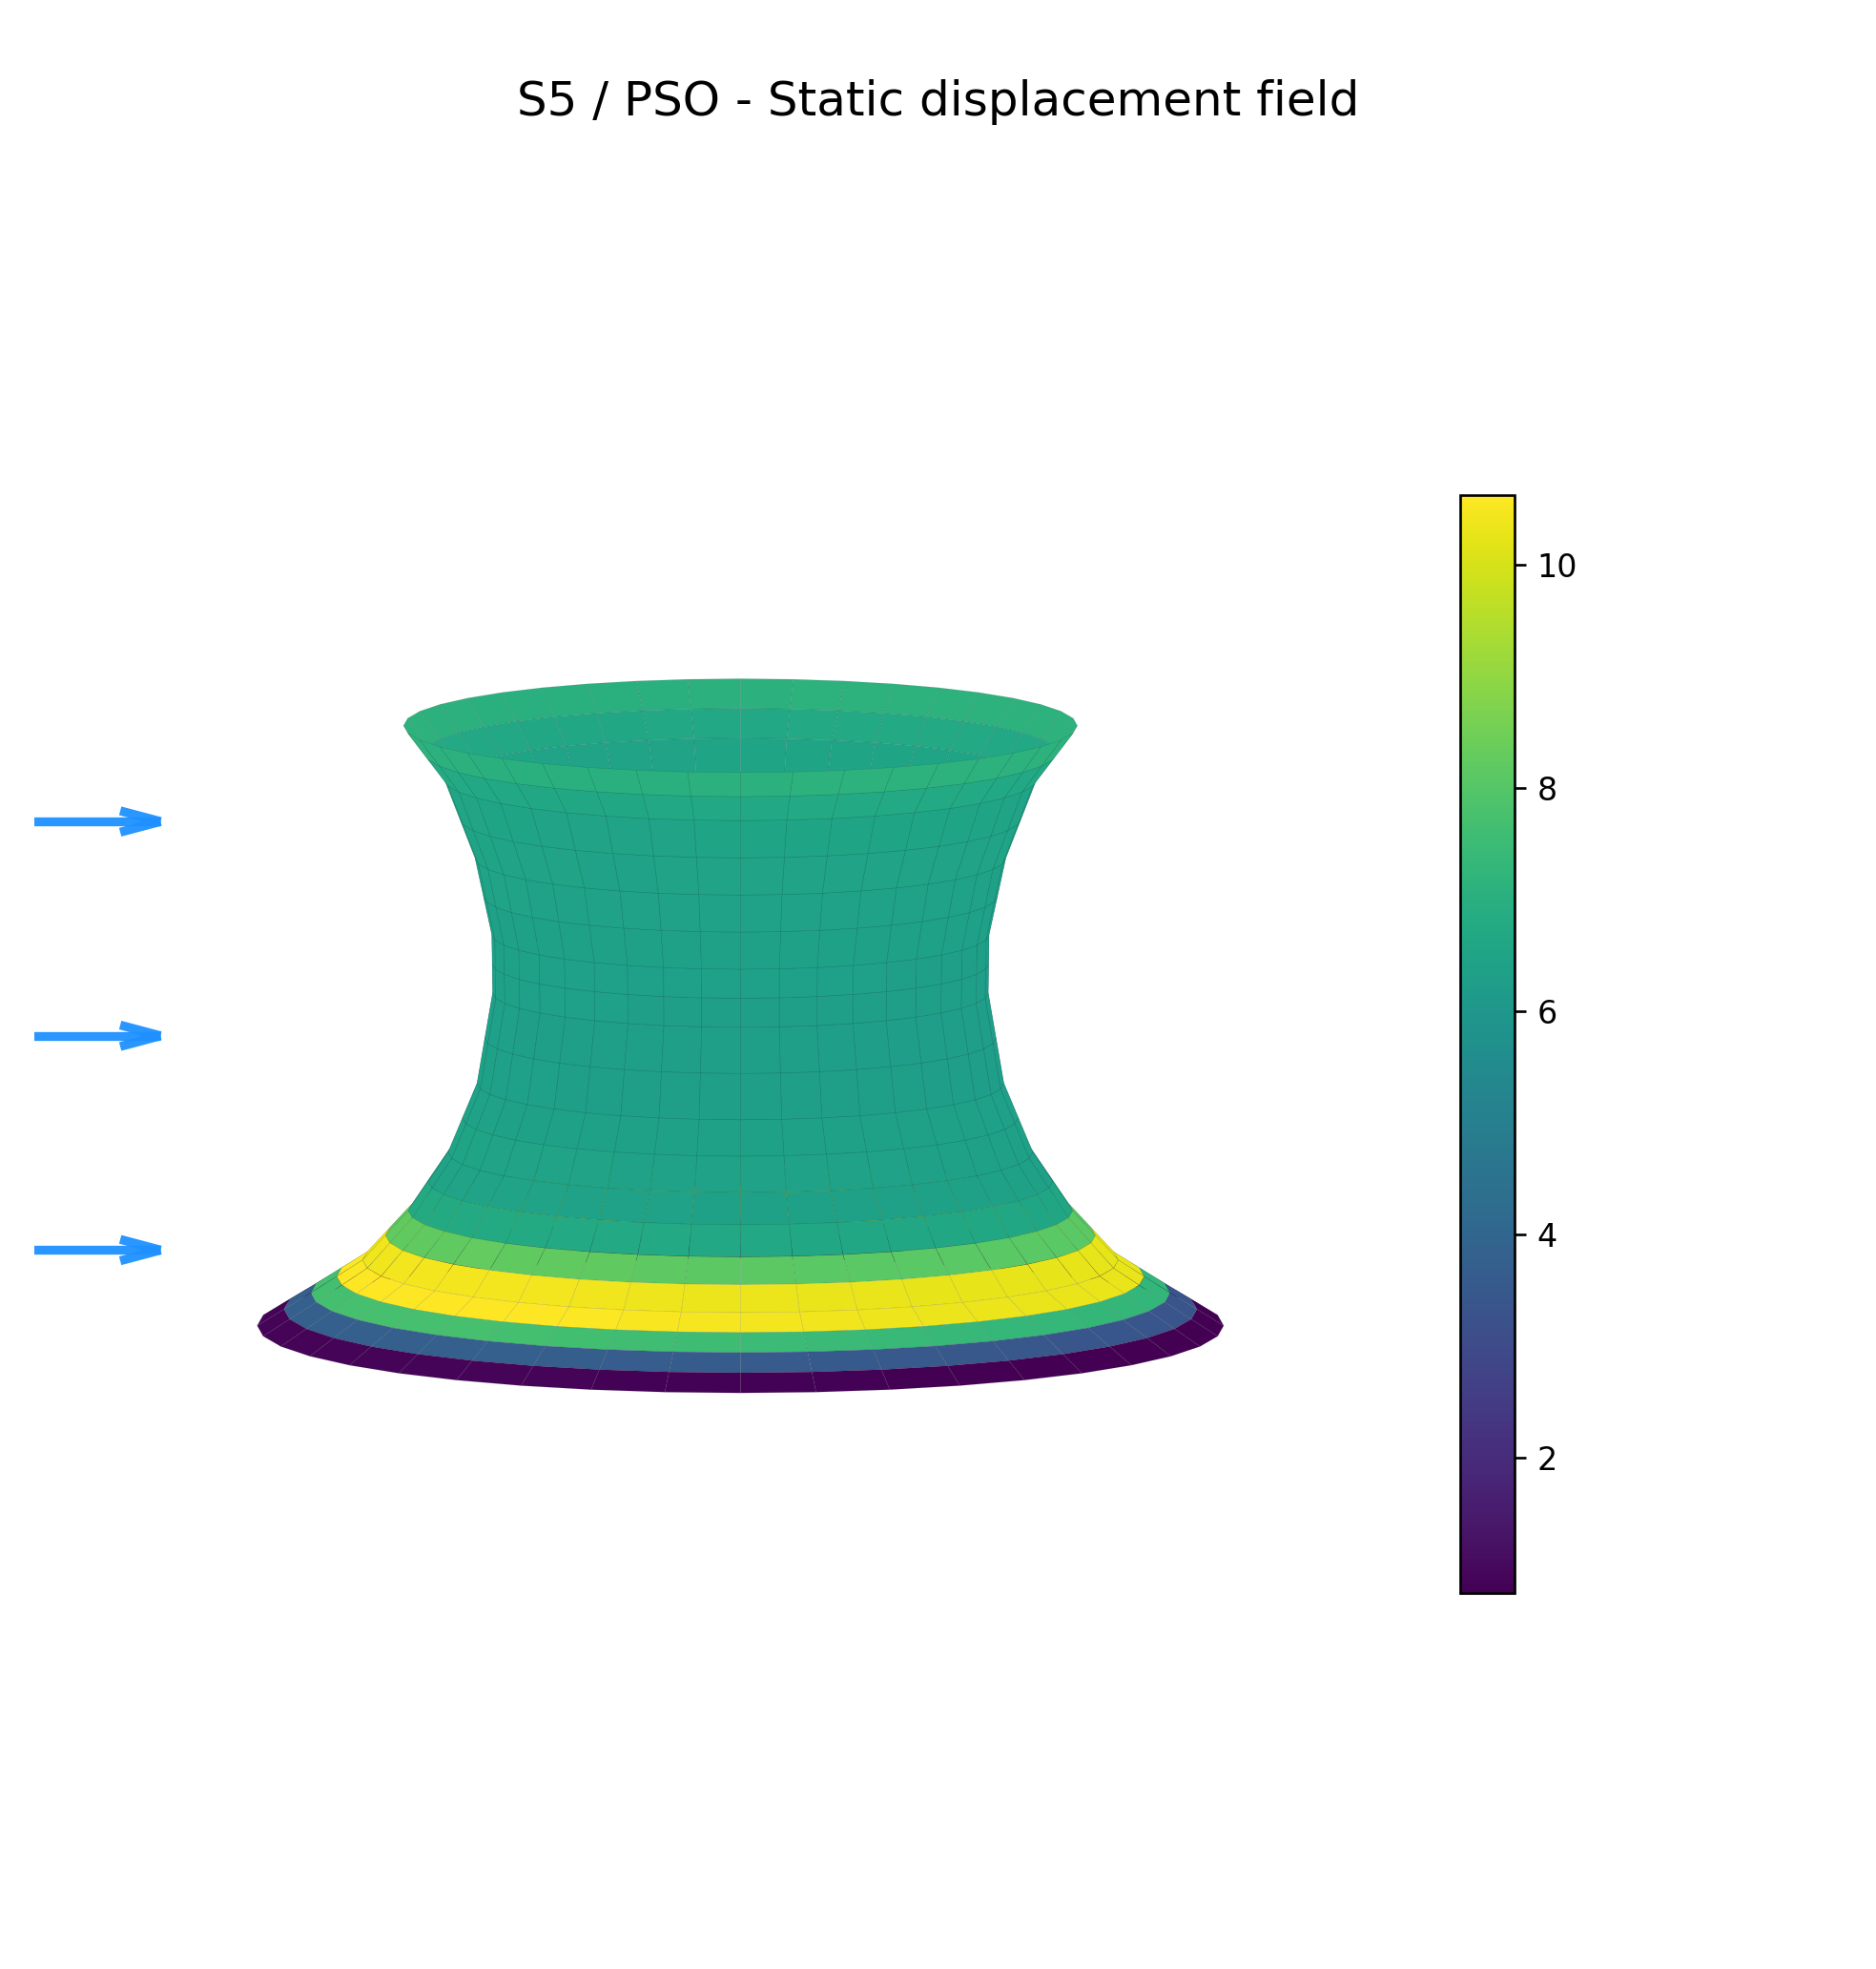
\includegraphics[width=\textwidth]{../results/figures/task7_s5_pso_displacement.png}
\caption{S5 / PSO displacement}
\end{subfigure}\hfill
\begin{subfigure}{0.32\textwidth}
\centering
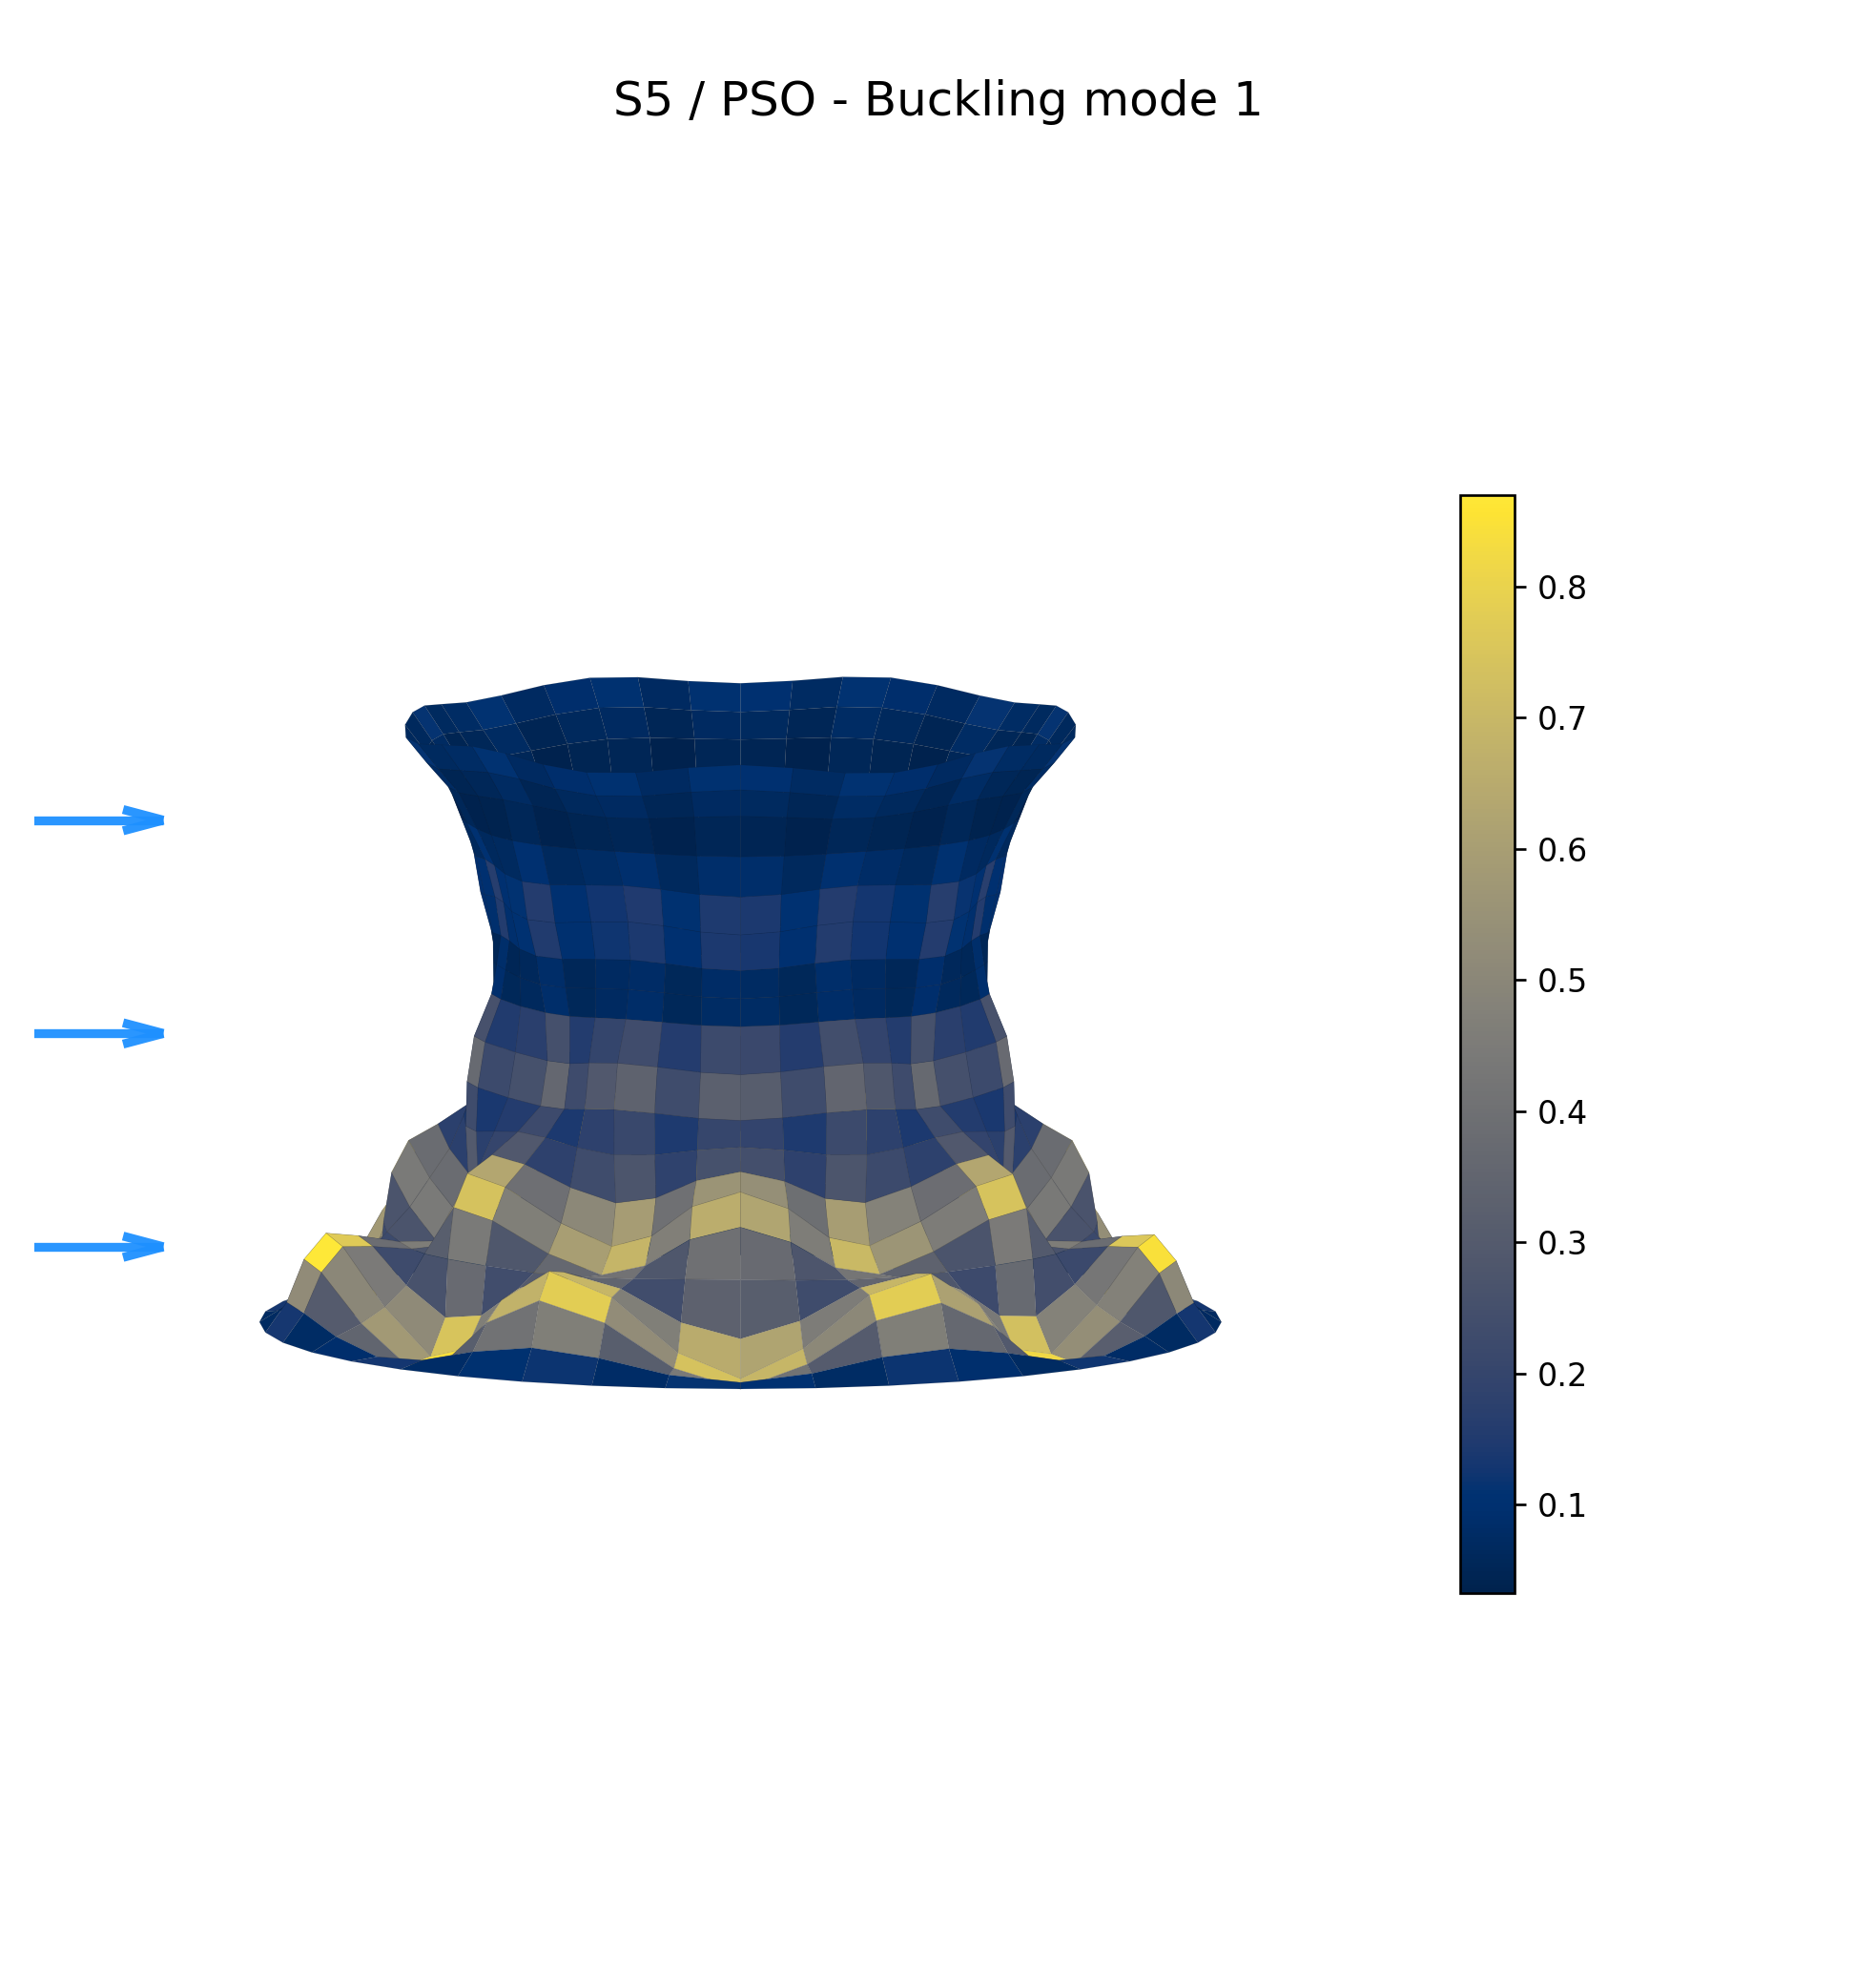
\includegraphics[width=\textwidth]{../results/figures/task7_s5_pso_buckling_mode1.png}
\caption{S5 / PSO buckling}
\end{subfigure}
\caption{Combined visual fields}
\end{figure}


\subsection{S5 / SA}


\begin{figure}[H]
\centering
\begin{subfigure}{0.32\textwidth}
\centering
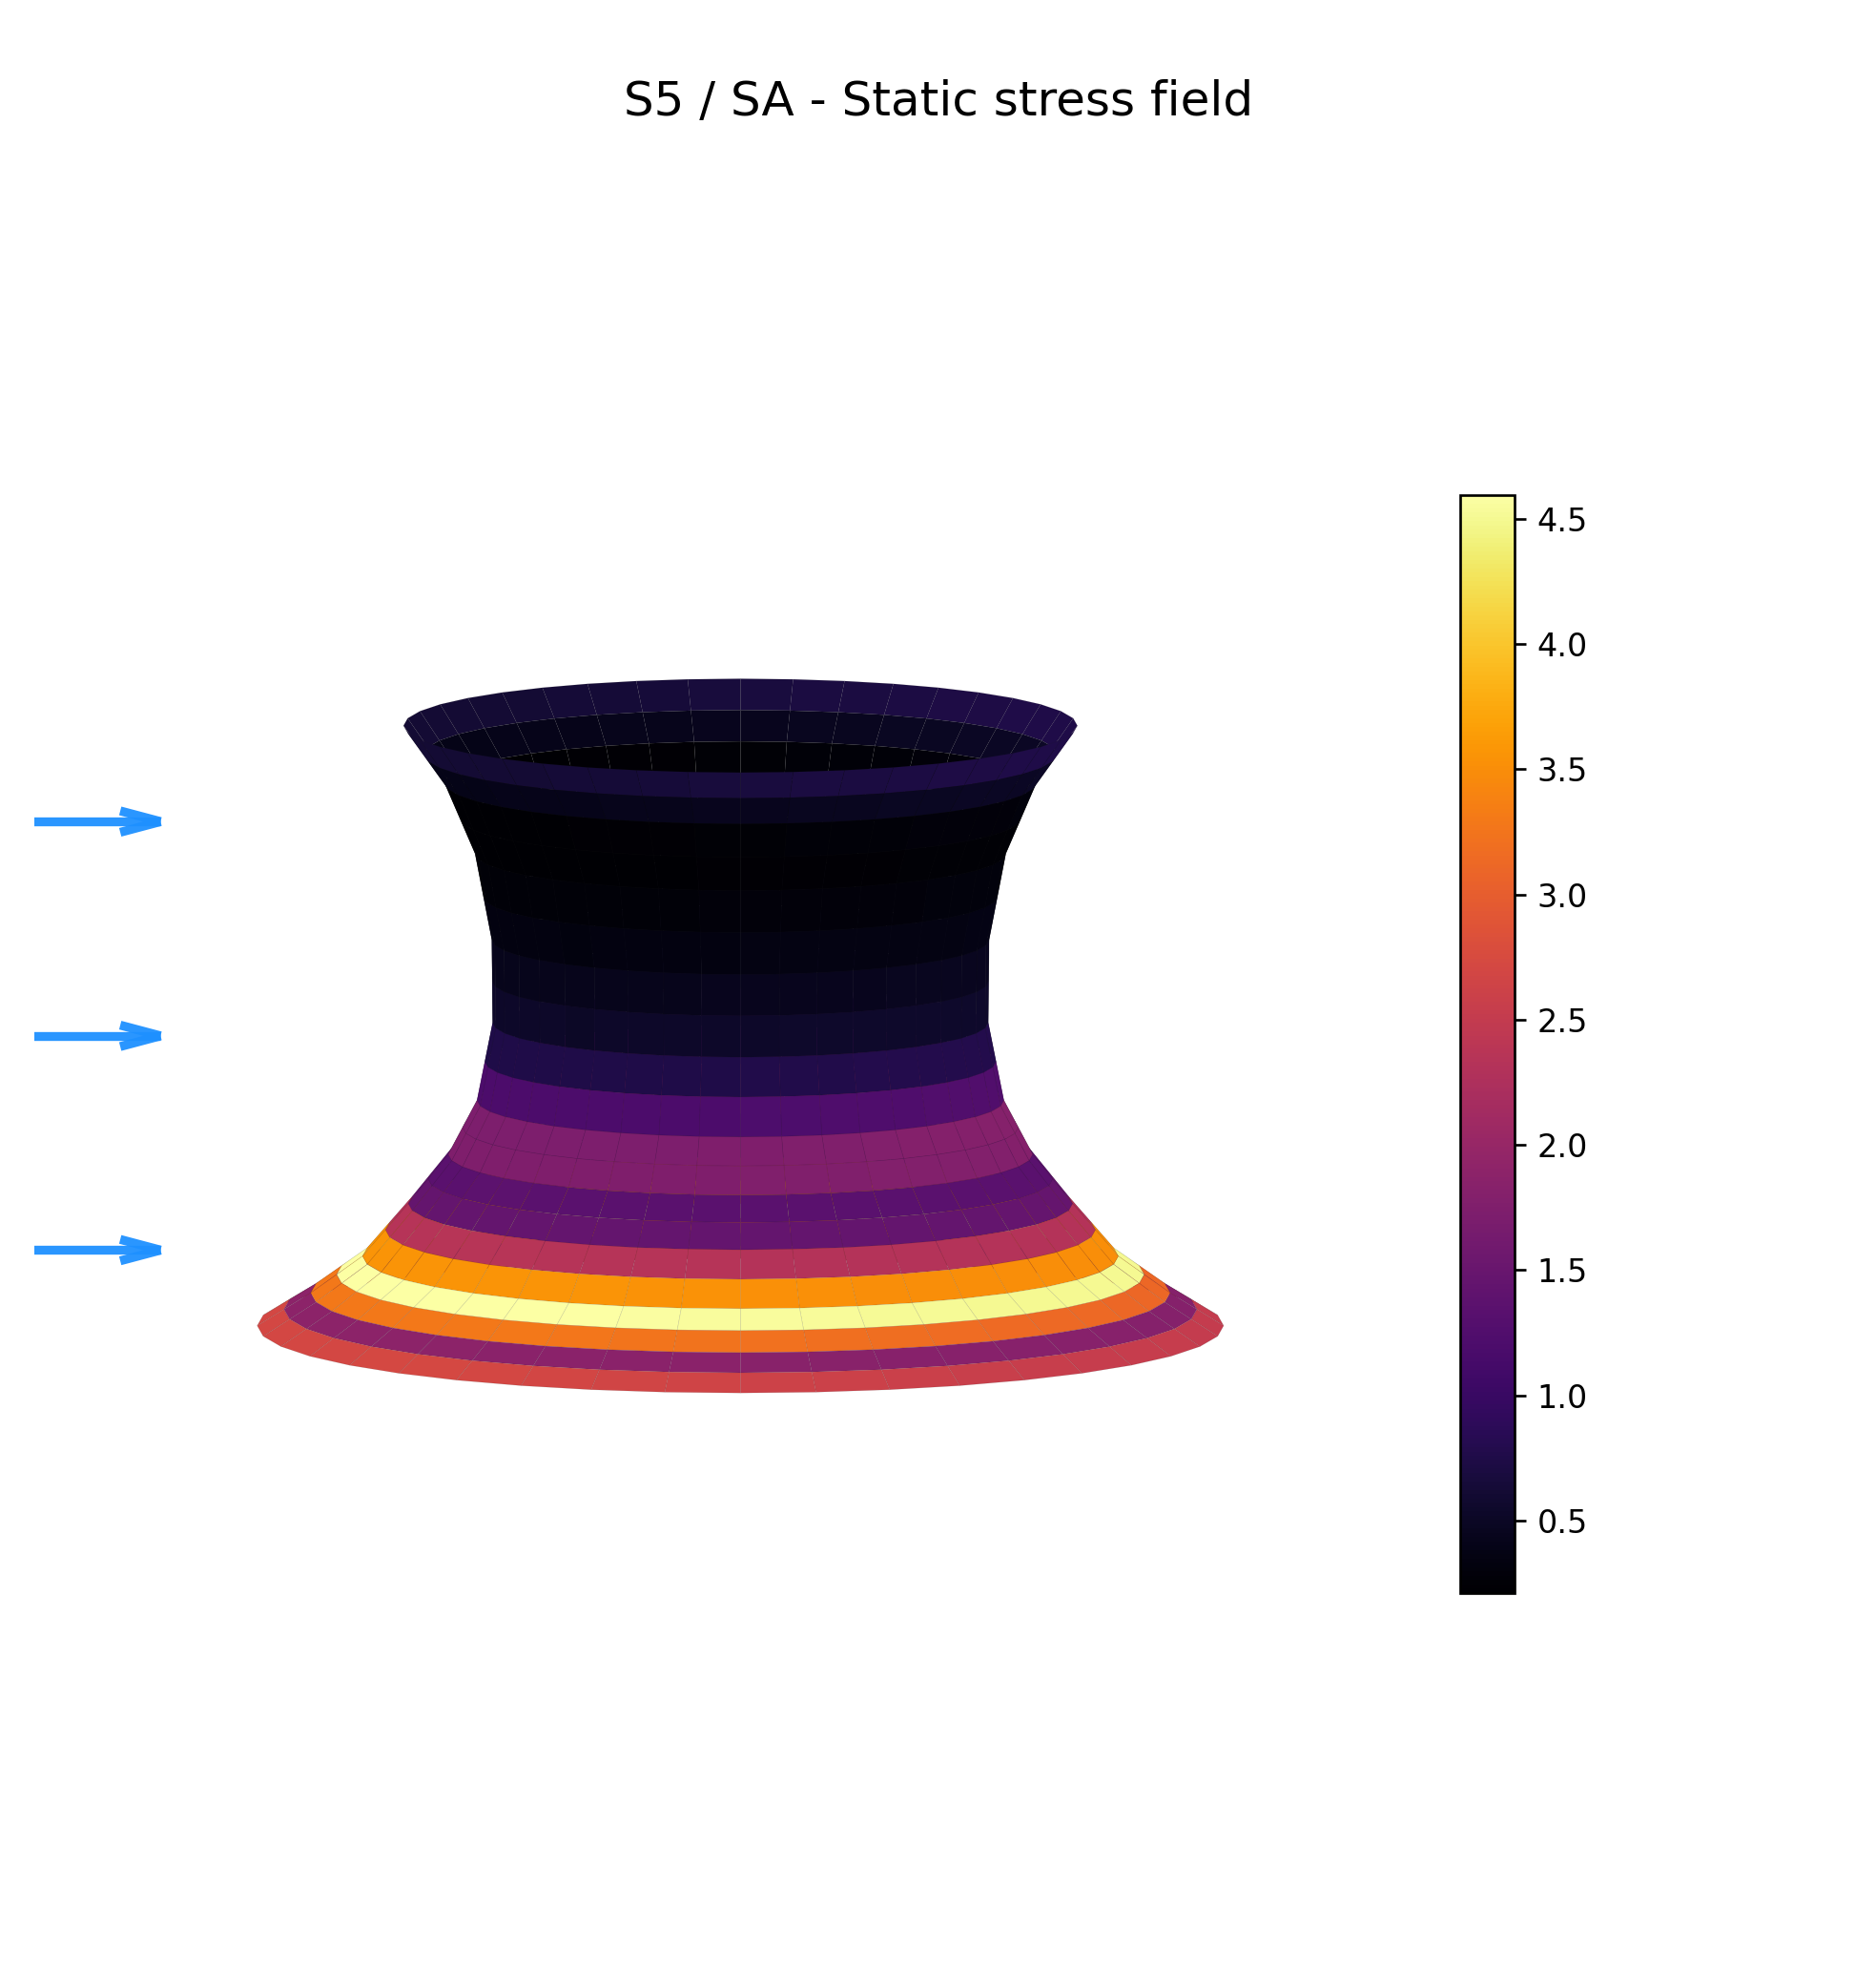
\includegraphics[width=\textwidth]{../results/figures/task7_s5_sa_stress.png}
\caption{S5 / SA stress}
\end{subfigure}\hfill
\begin{subfigure}{0.32\textwidth}
\centering
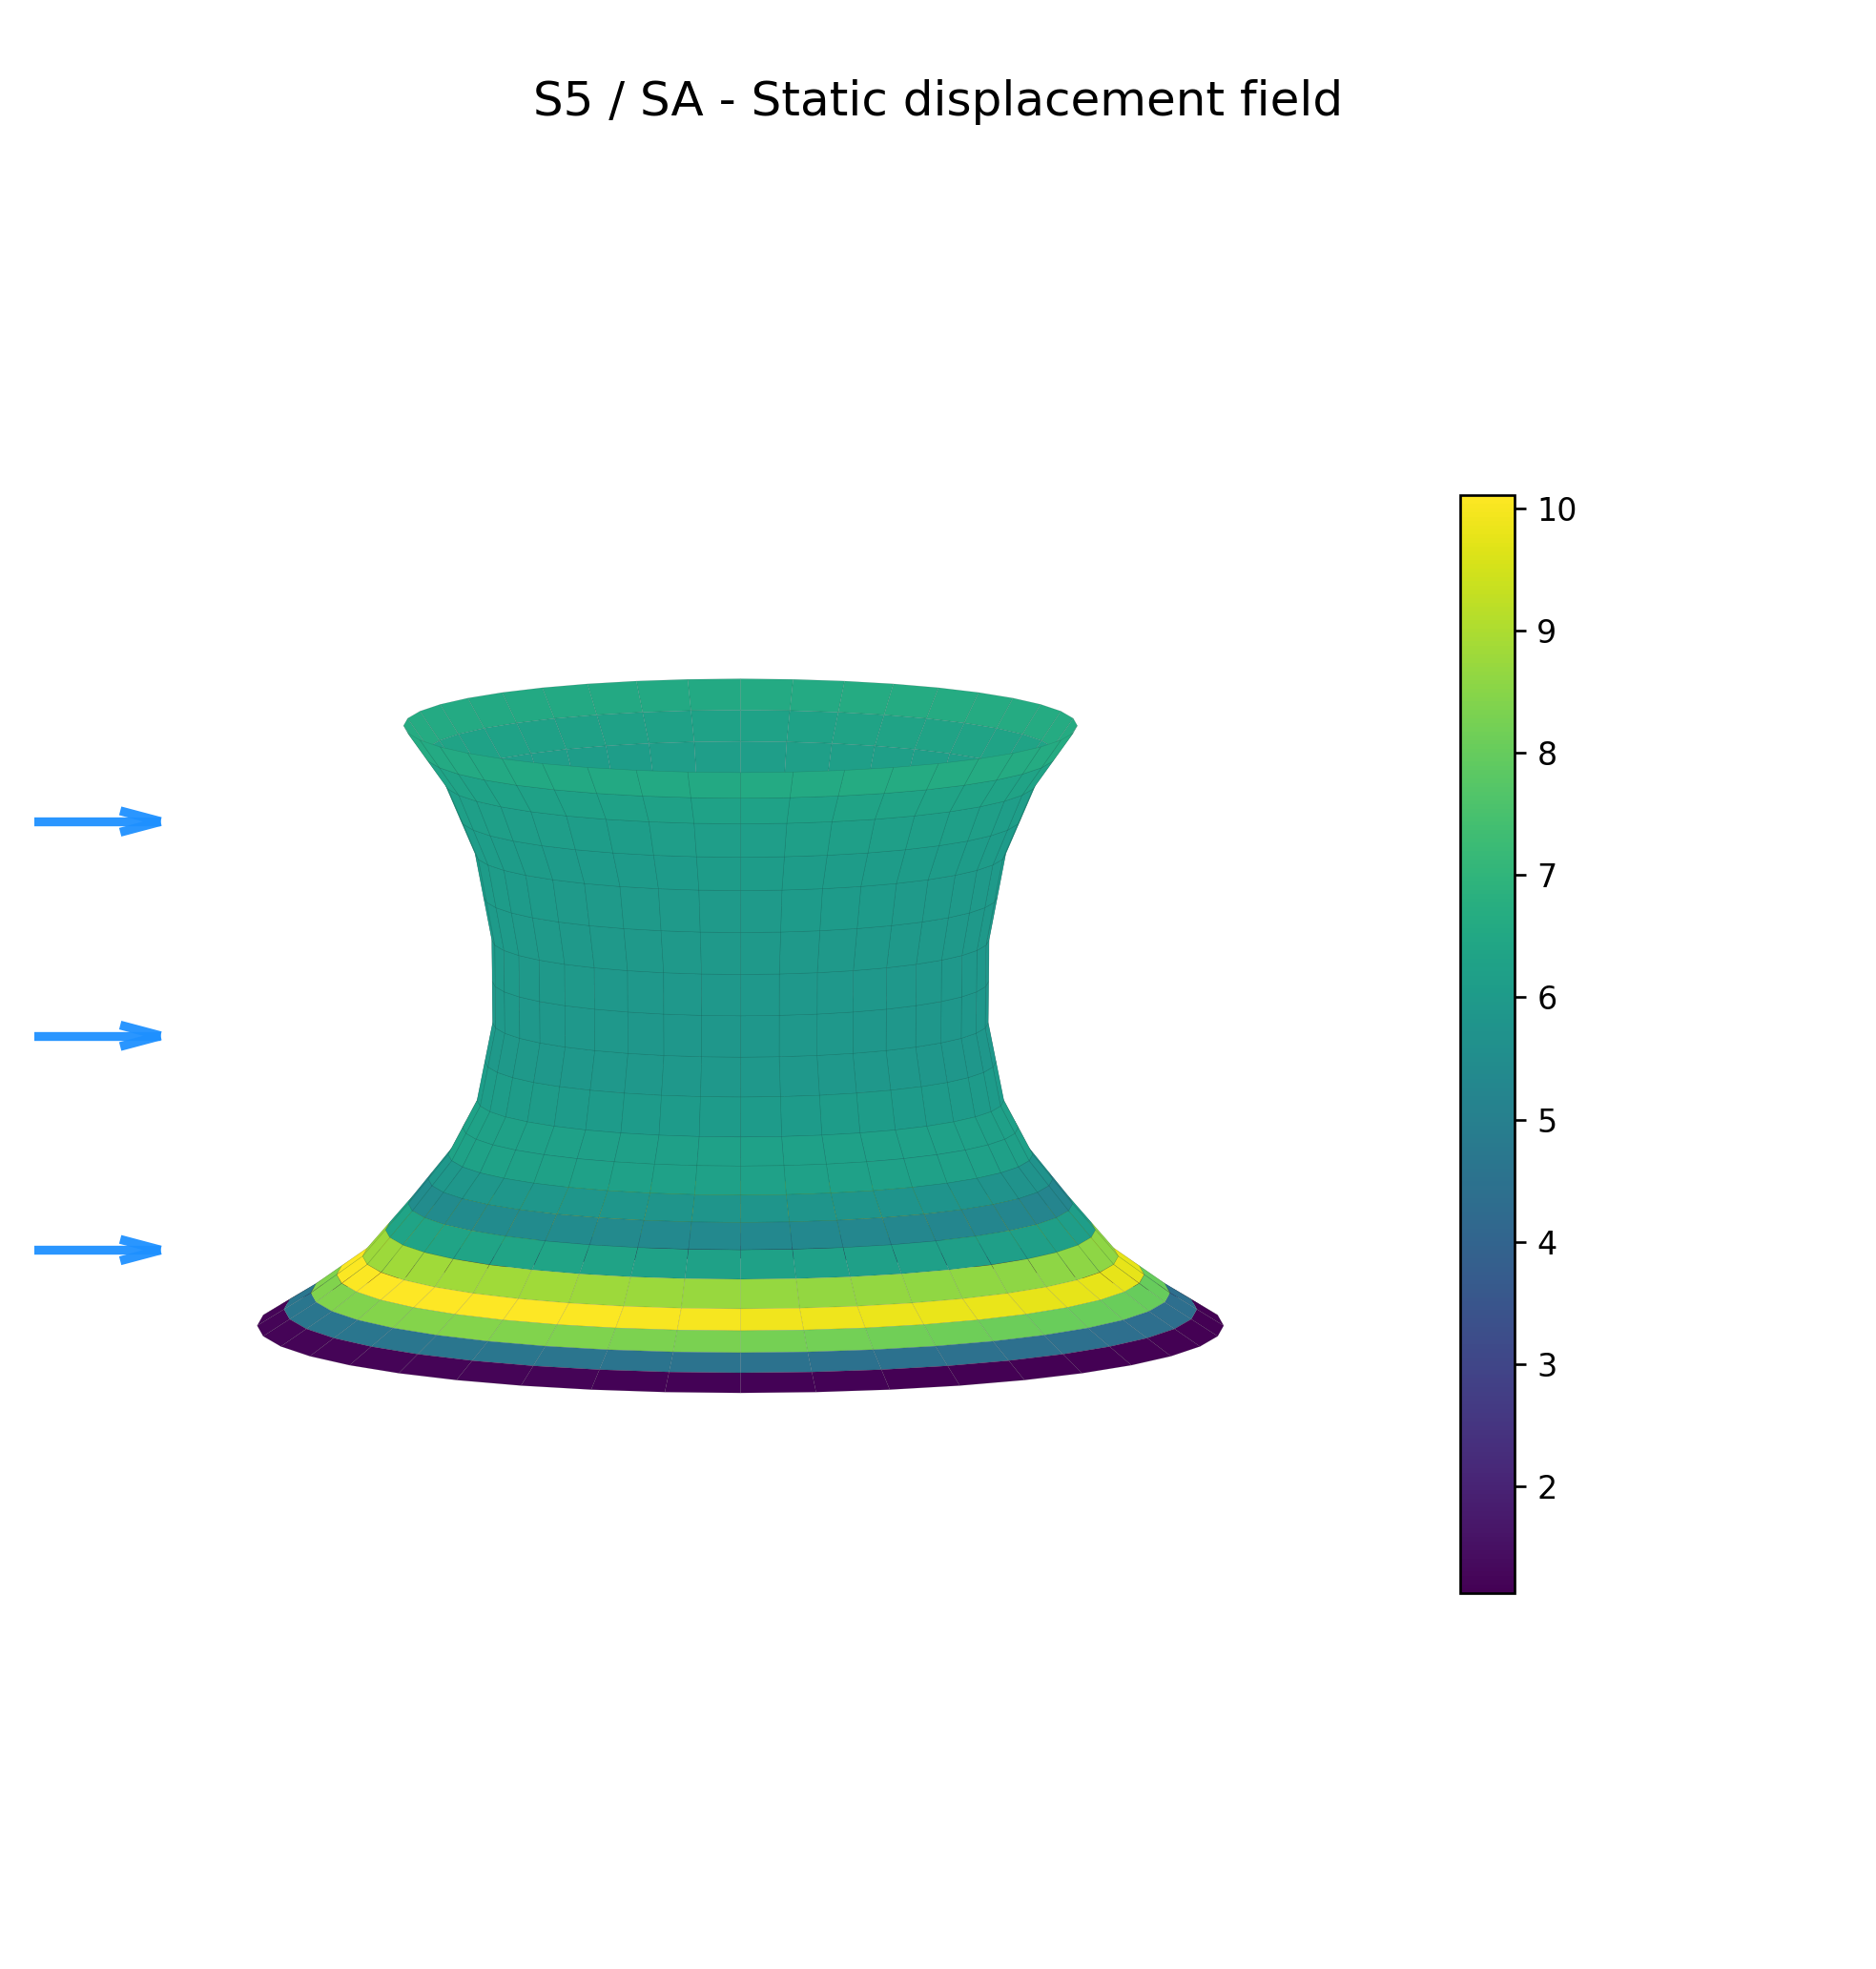
\includegraphics[width=\textwidth]{../results/figures/task7_s5_sa_displacement.png}
\caption{S5 / SA displacement}
\end{subfigure}\hfill
\begin{subfigure}{0.32\textwidth}
\centering
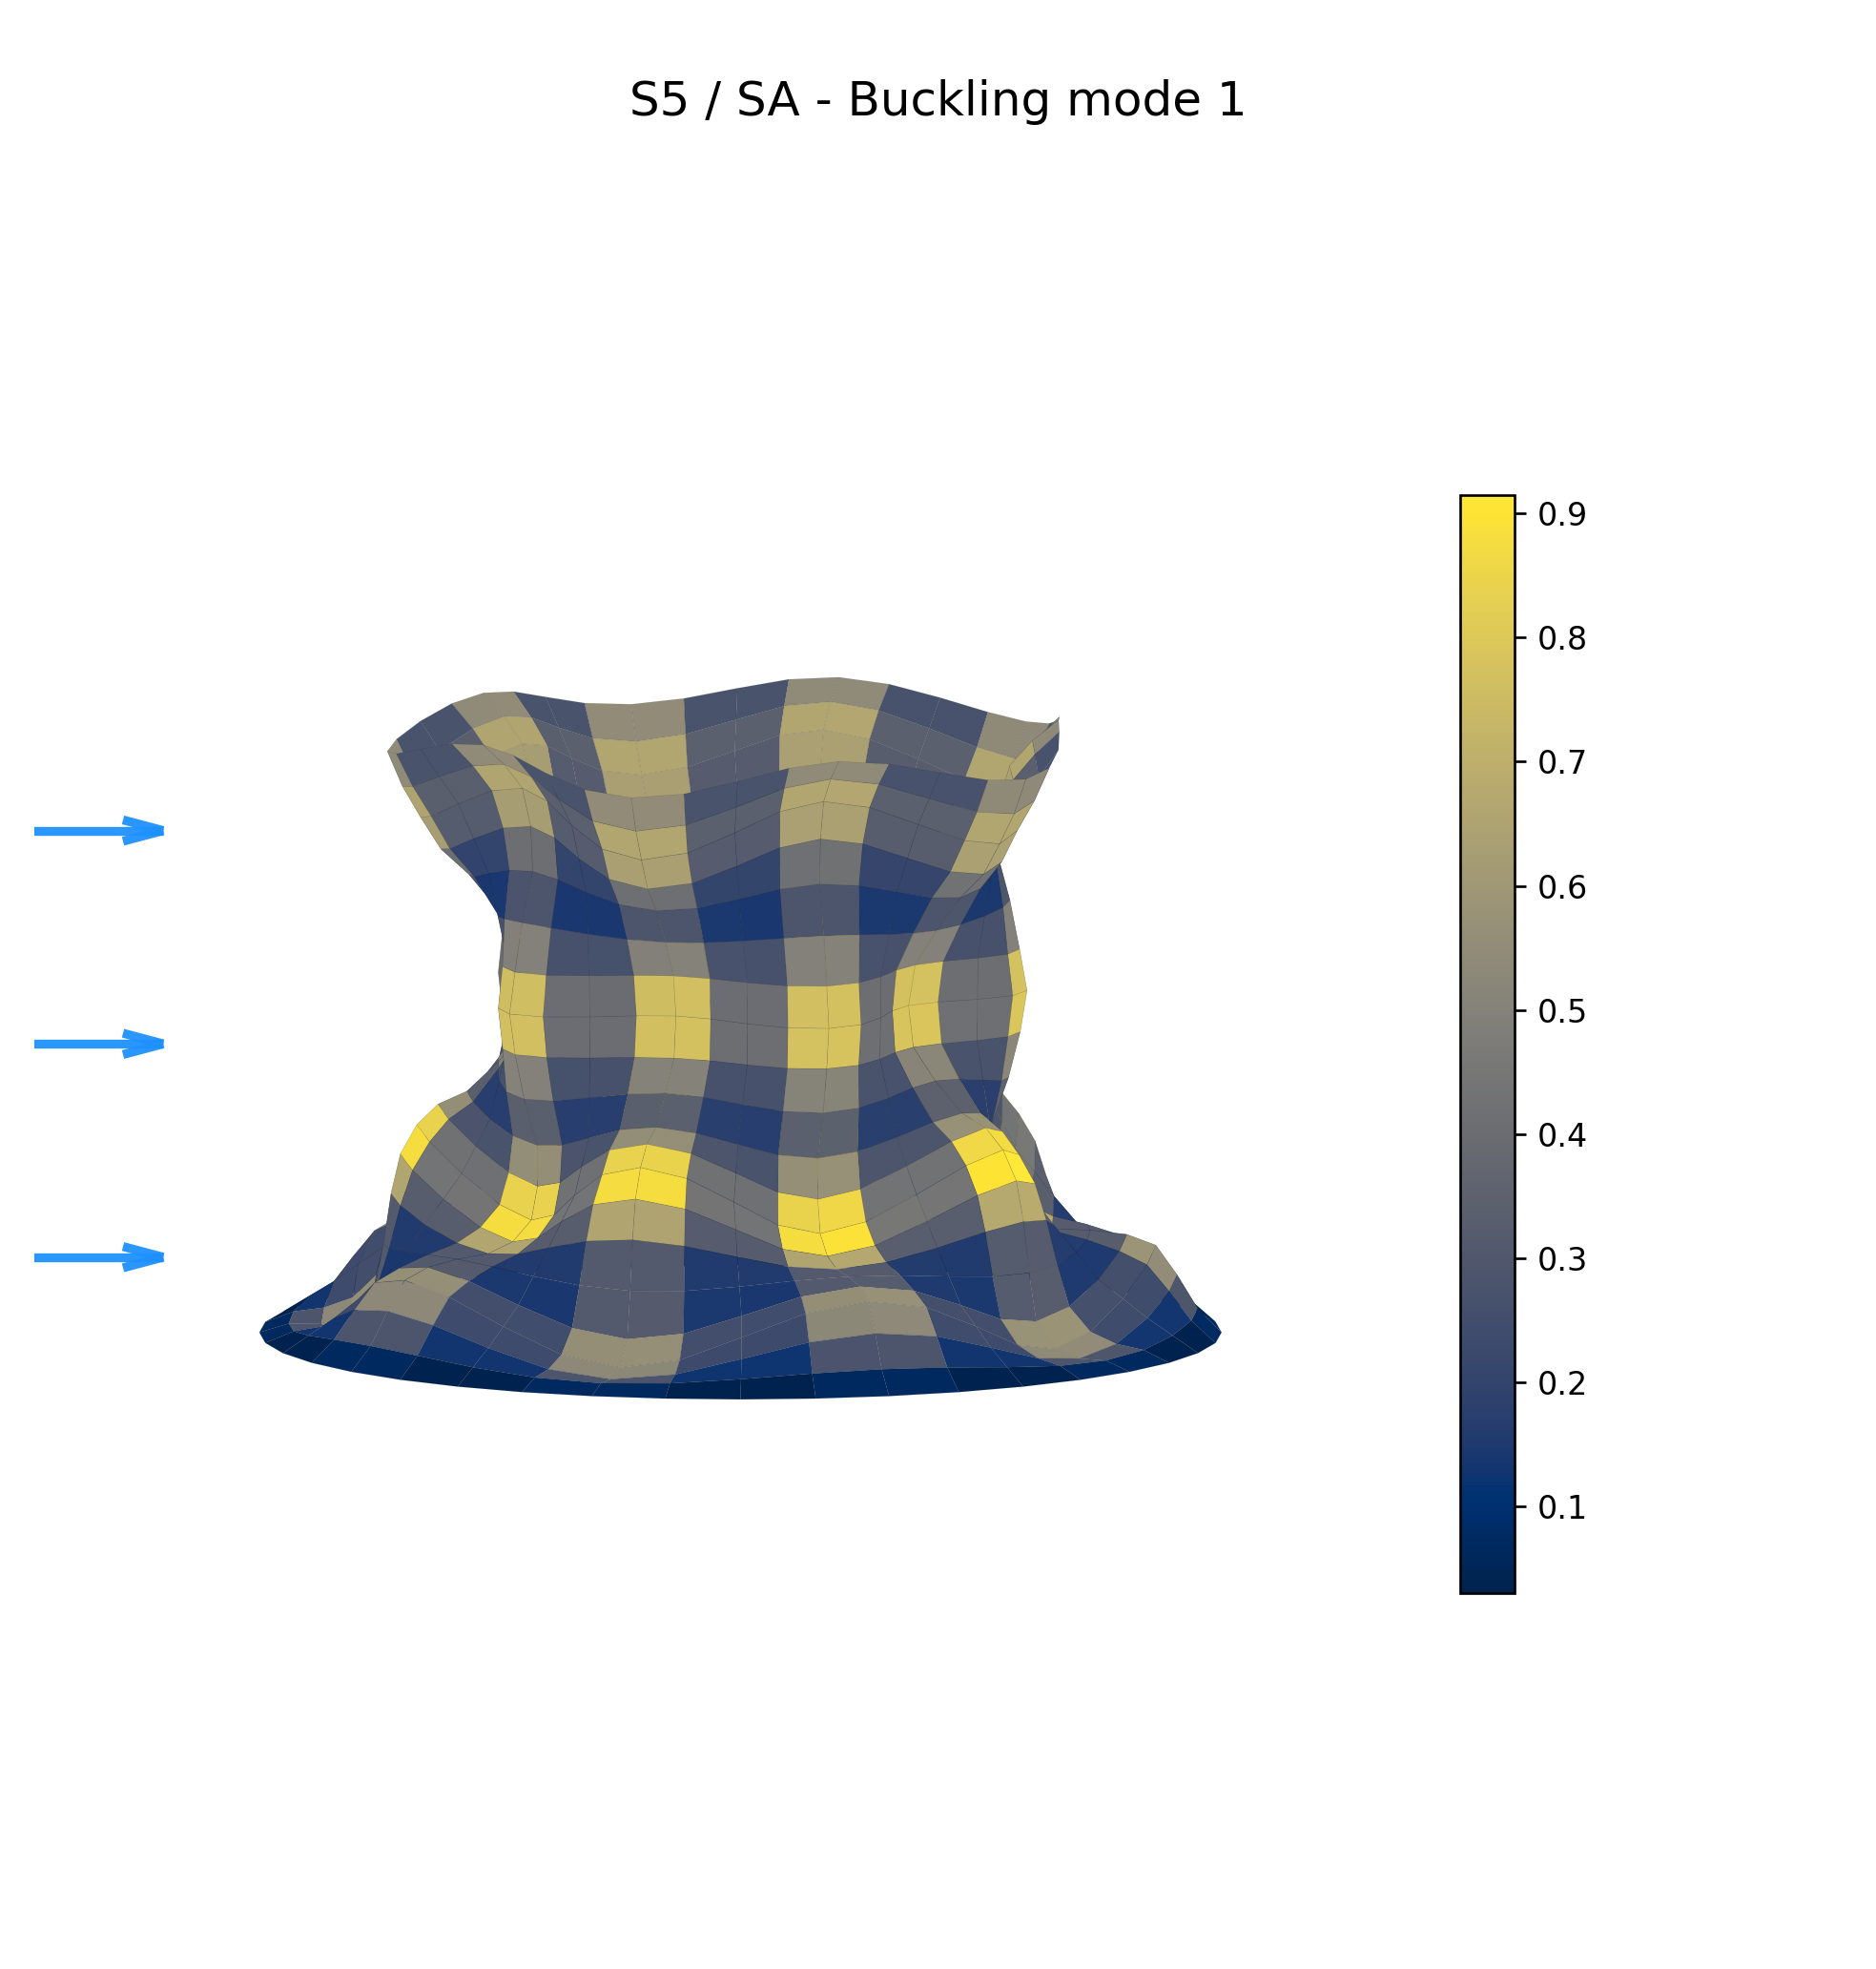
\includegraphics[width=\textwidth]{../results/figures/task7_s5_sa_buckling_mode1.png}
\caption{S5 / SA buckling}
\end{subfigure}
\caption{Combined visual fields}
\end{figure}


\section{Scenario S6}


\subsection{S6 / BFGS}


\begin{figure}[H]
\centering
\begin{subfigure}{0.32\textwidth}
\centering
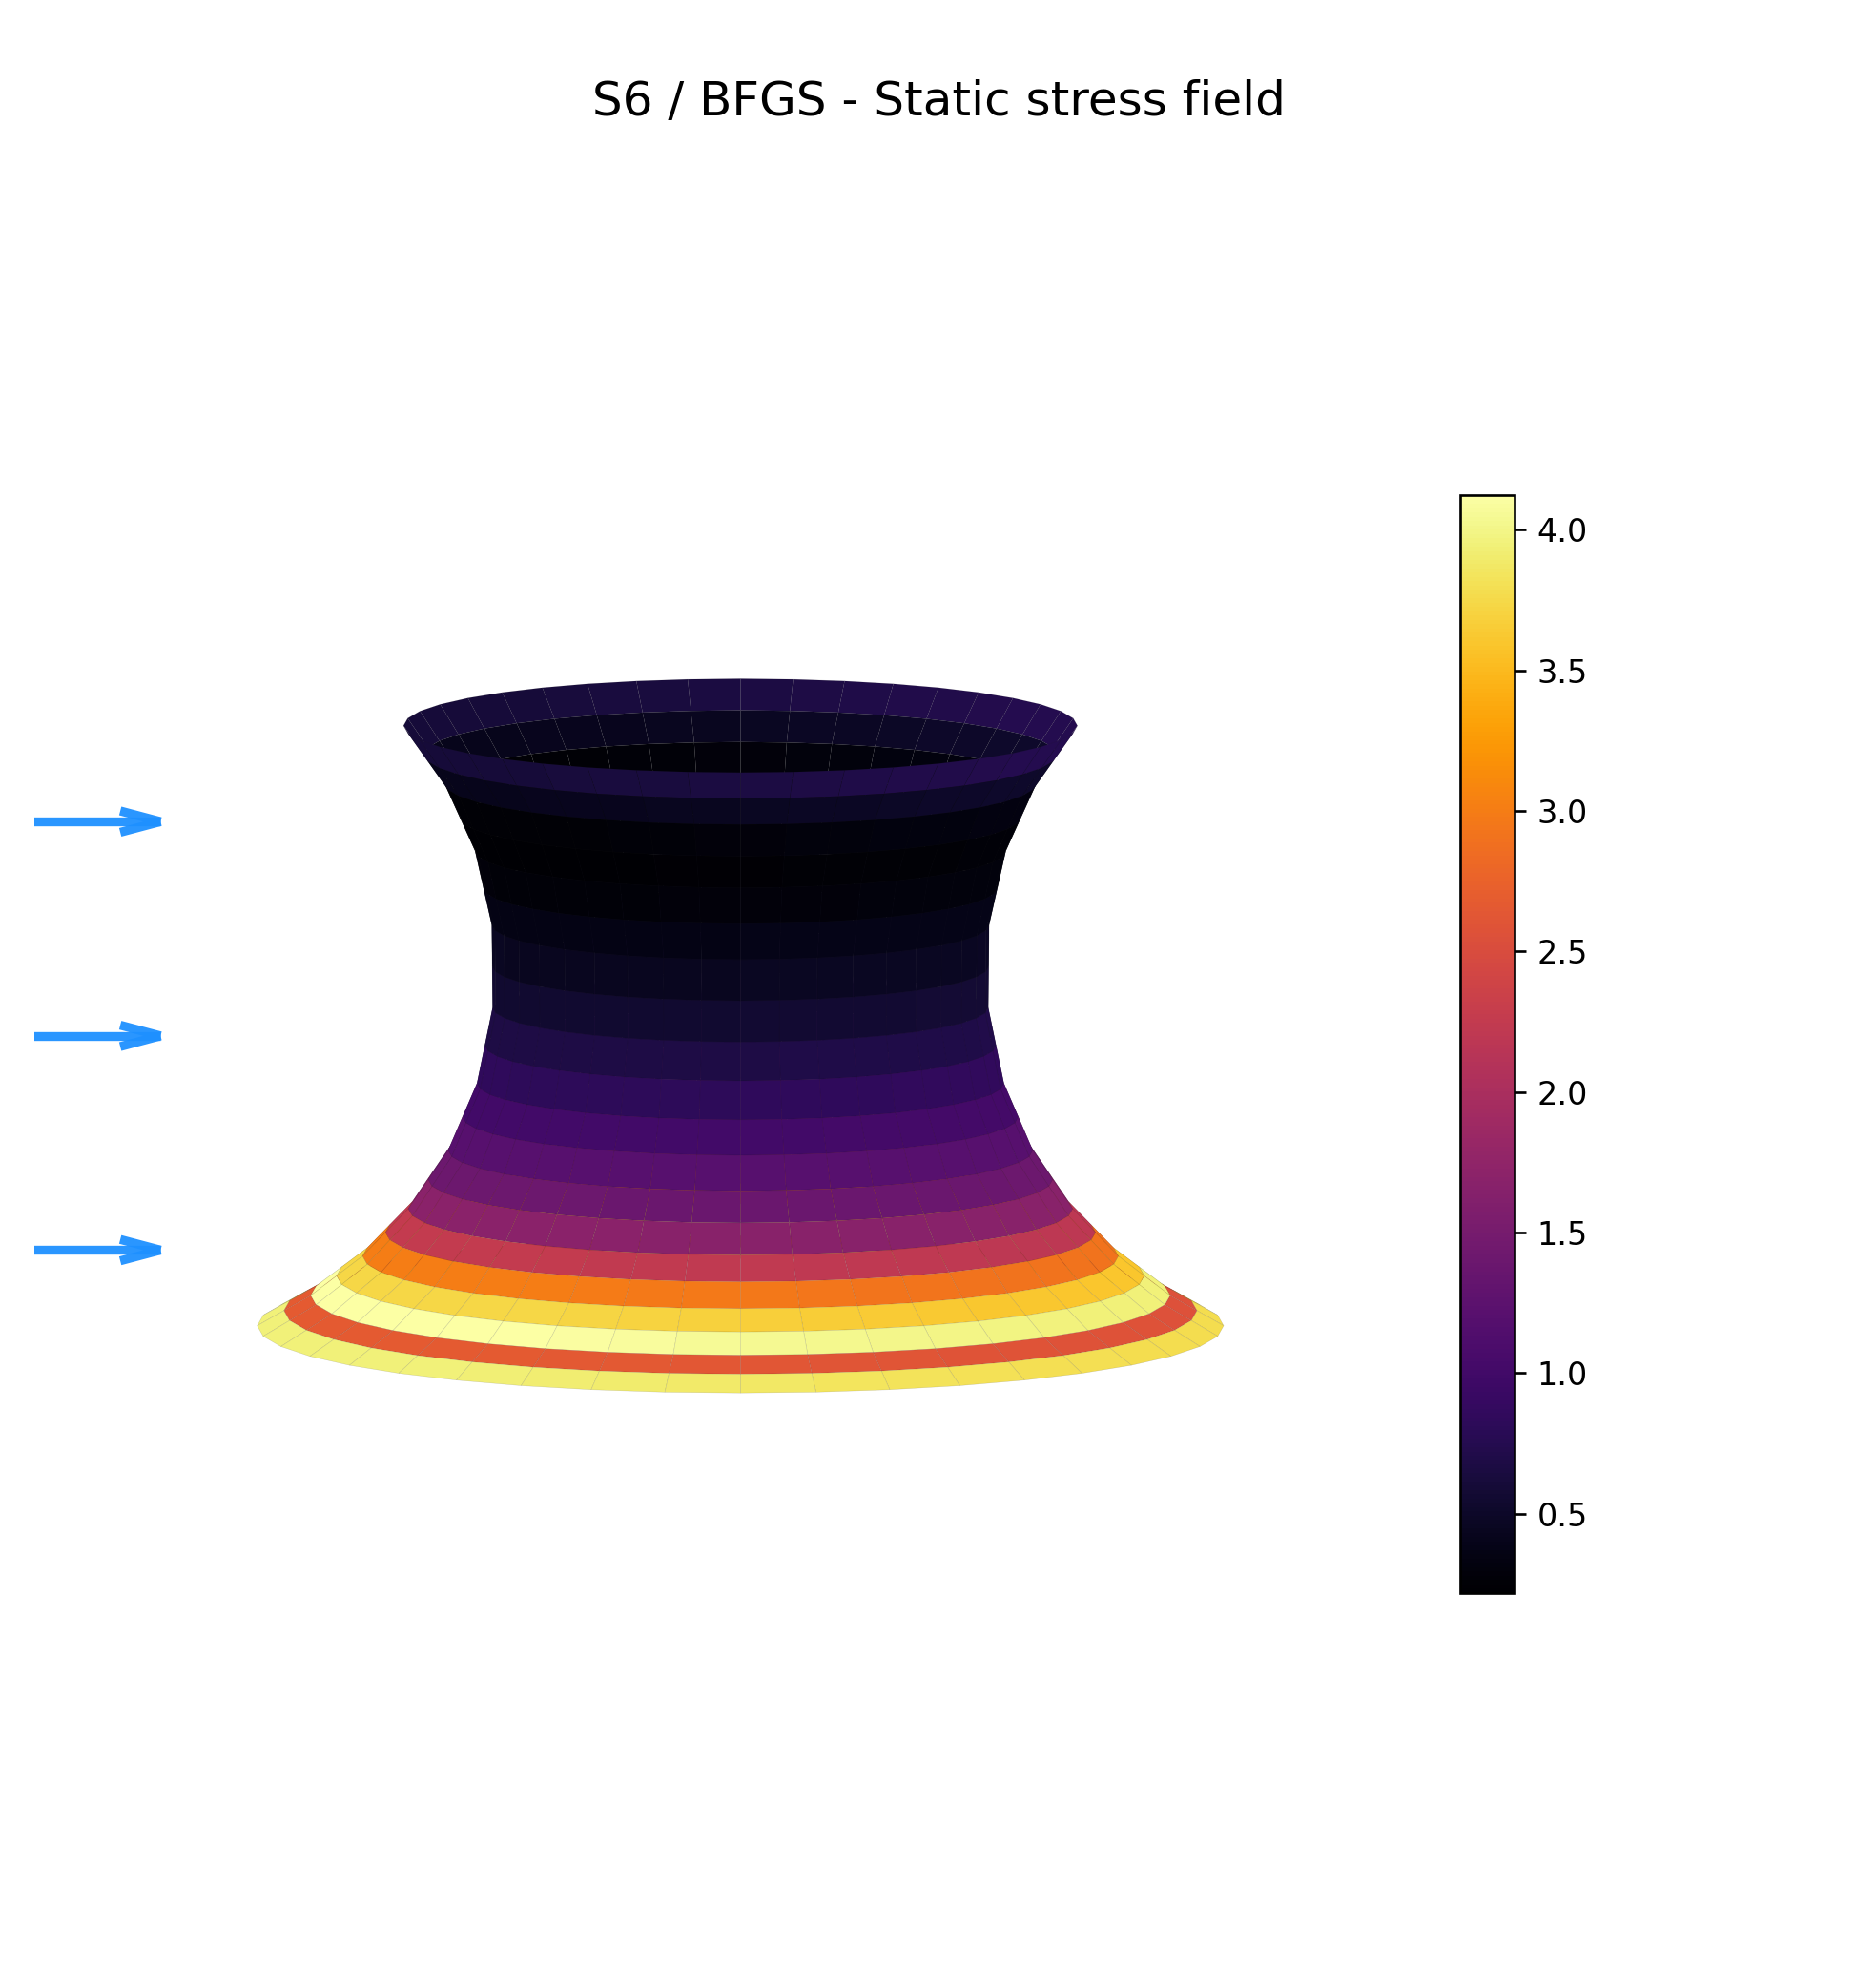
\includegraphics[width=\textwidth]{../results/figures/task7_s6_bfgs_stress.png}
\caption{S6 / BFGS stress}
\end{subfigure}\hfill
\begin{subfigure}{0.32\textwidth}
\centering
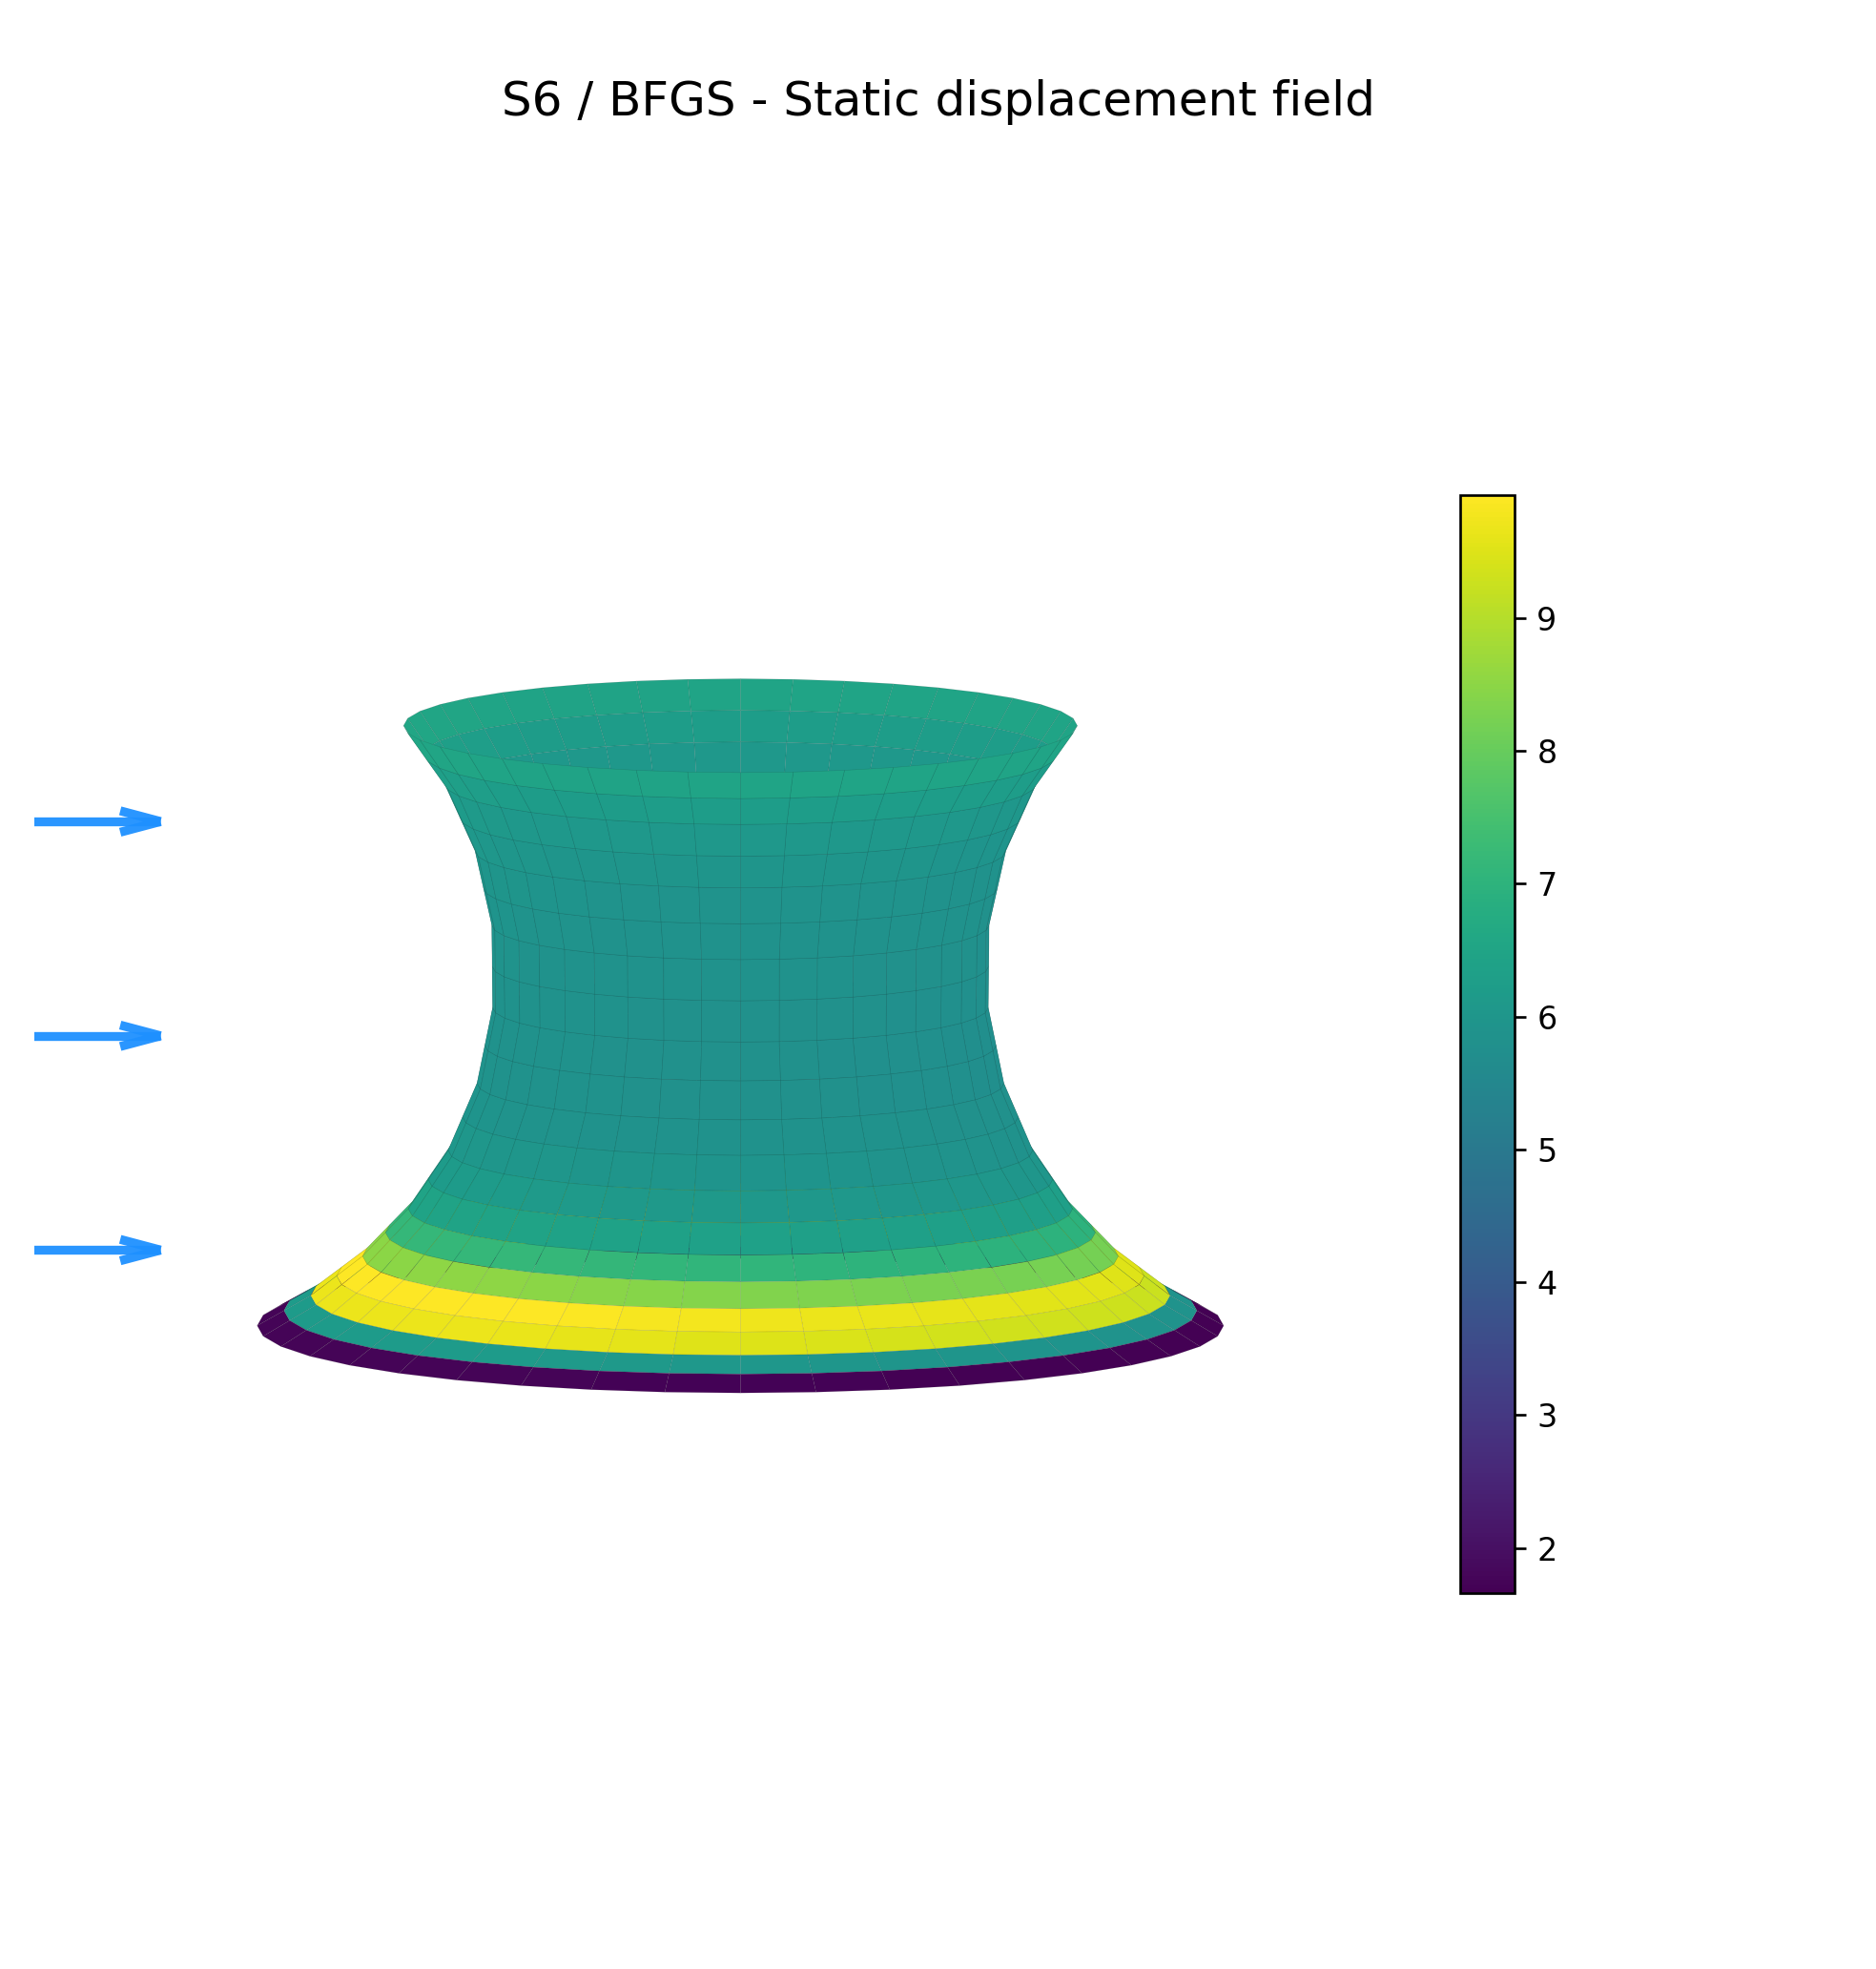
\includegraphics[width=\textwidth]{../results/figures/task7_s6_bfgs_displacement.png}
\caption{S6 / BFGS displacement}
\end{subfigure}\hfill
\begin{subfigure}{0.32\textwidth}
\centering
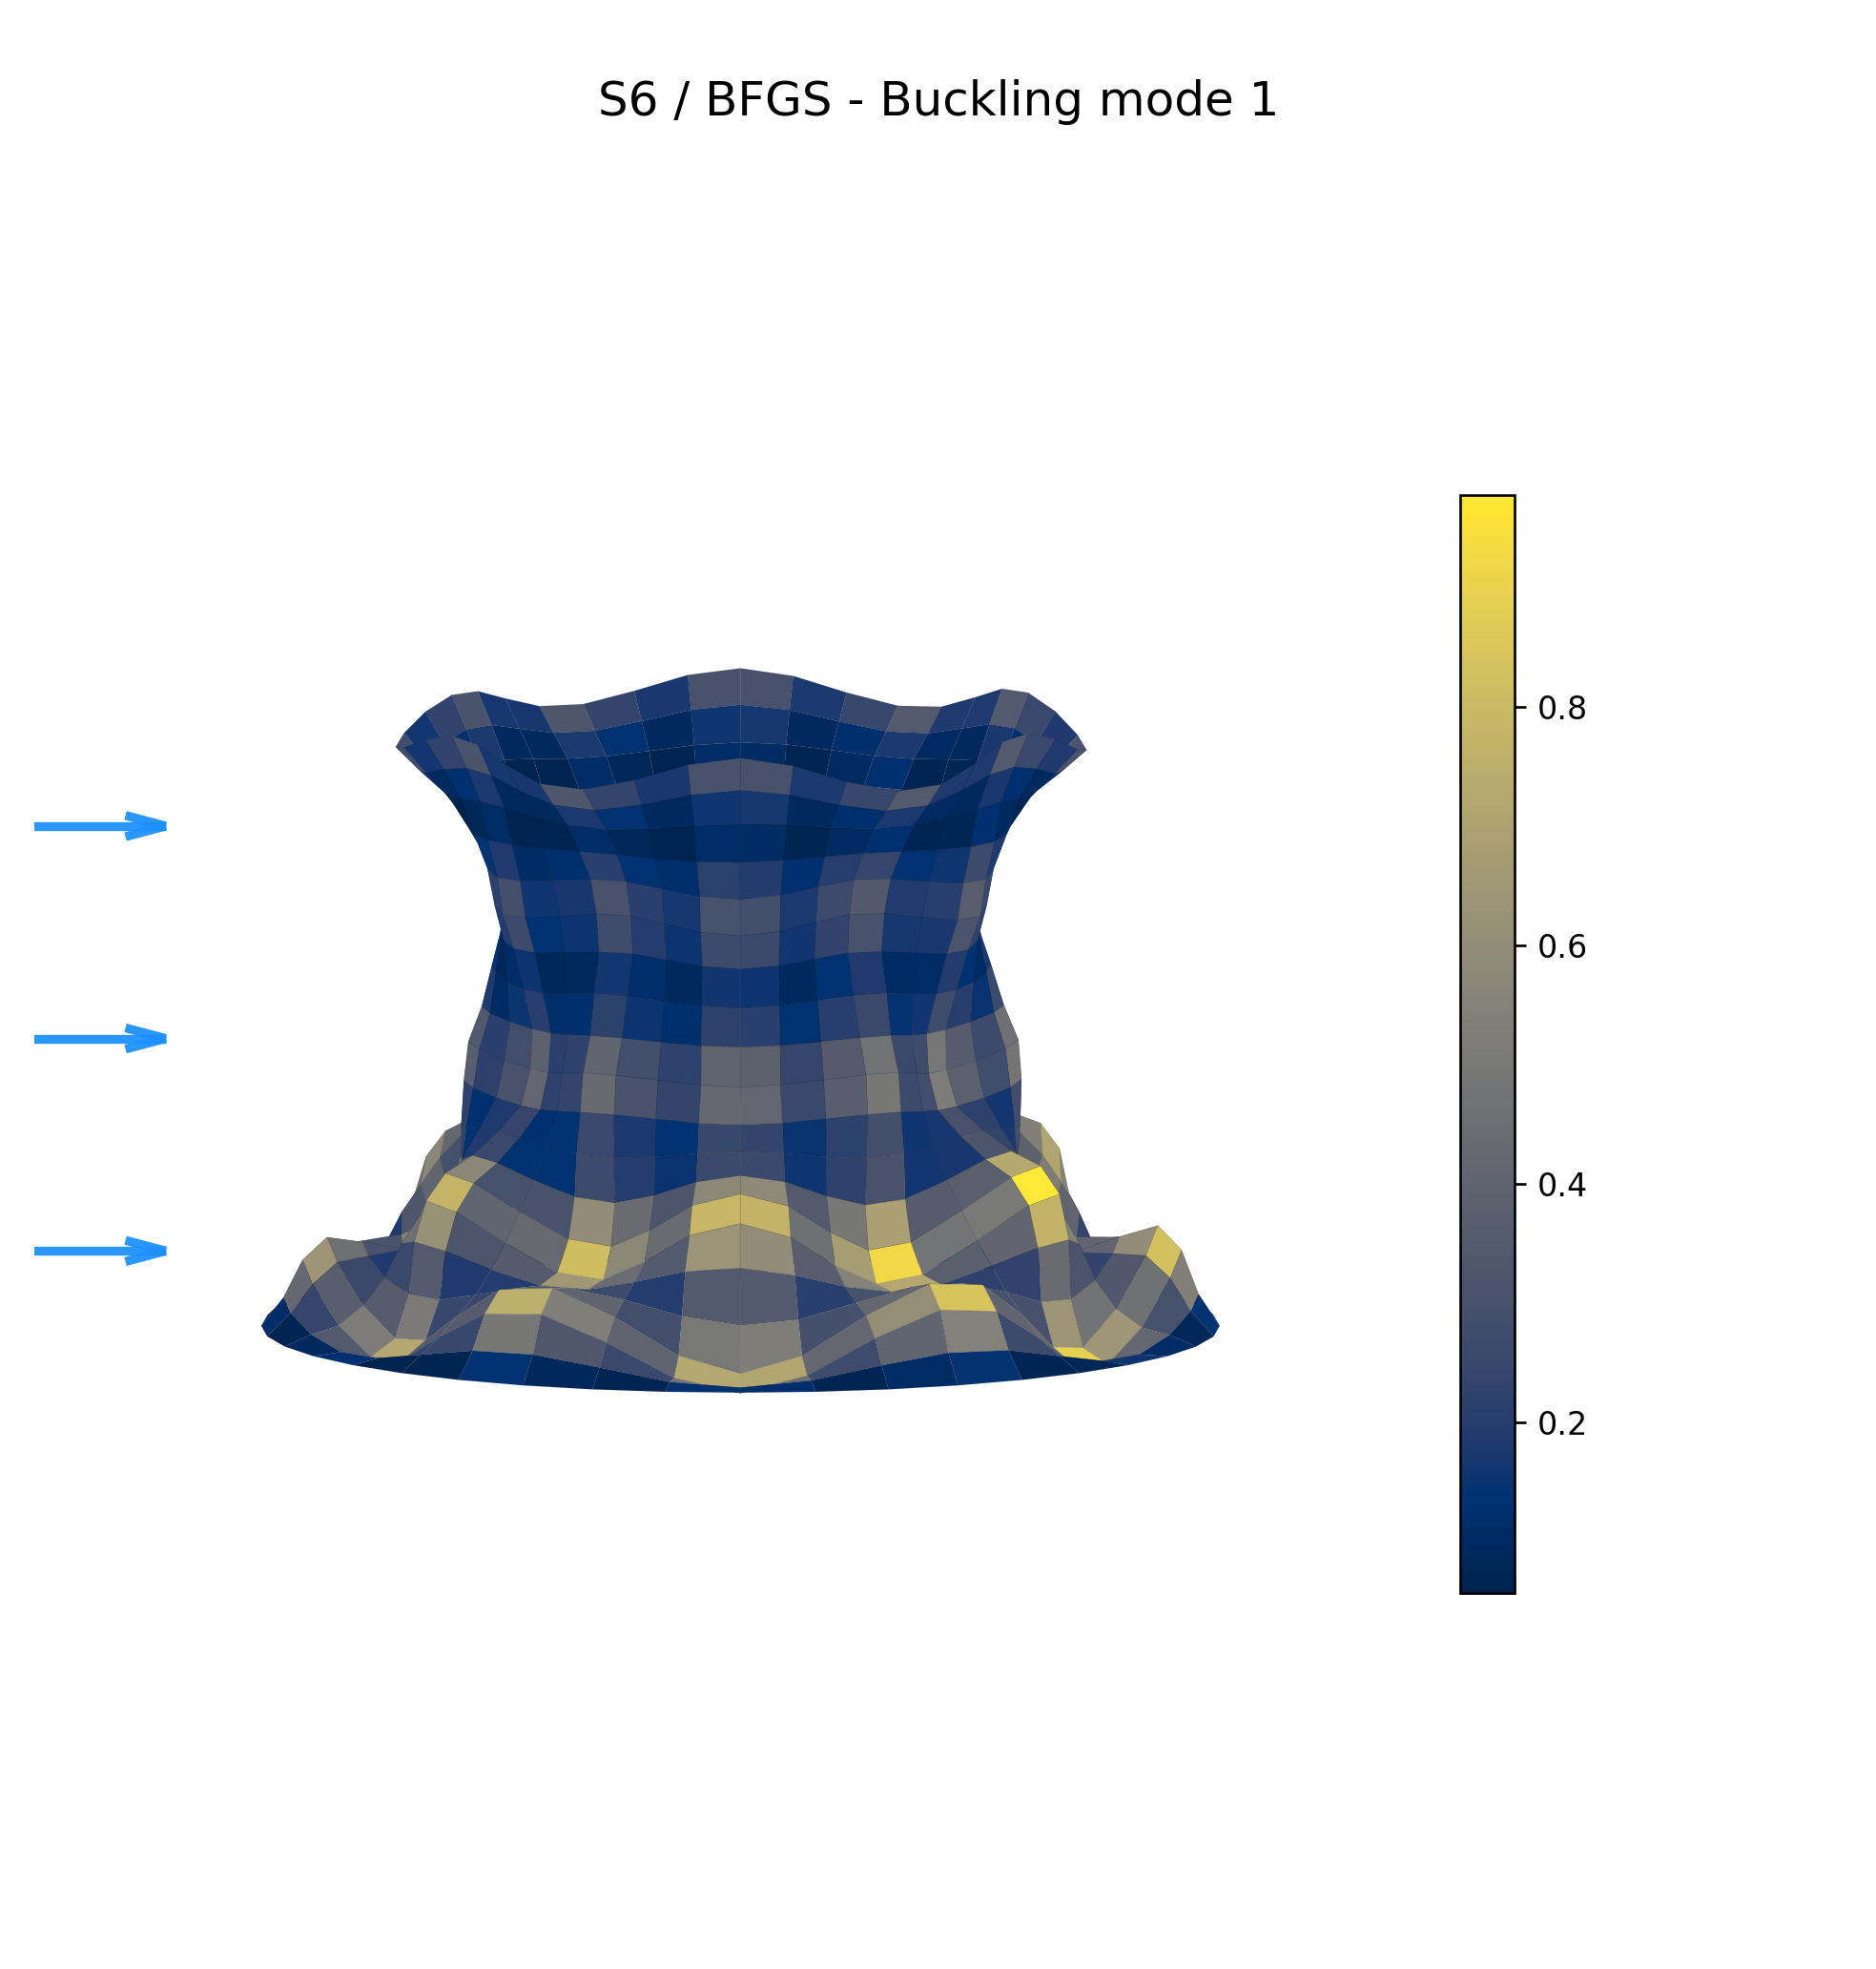
\includegraphics[width=\textwidth]{../results/figures/task7_s6_bfgs_buckling_mode1.png}
\caption{S6 / BFGS buckling}
\end{subfigure}
\caption{Combined visual fields}
\end{figure}


\subsection{S6 / PSO}


\begin{figure}[H]
\centering
\begin{subfigure}{0.32\textwidth}
\centering
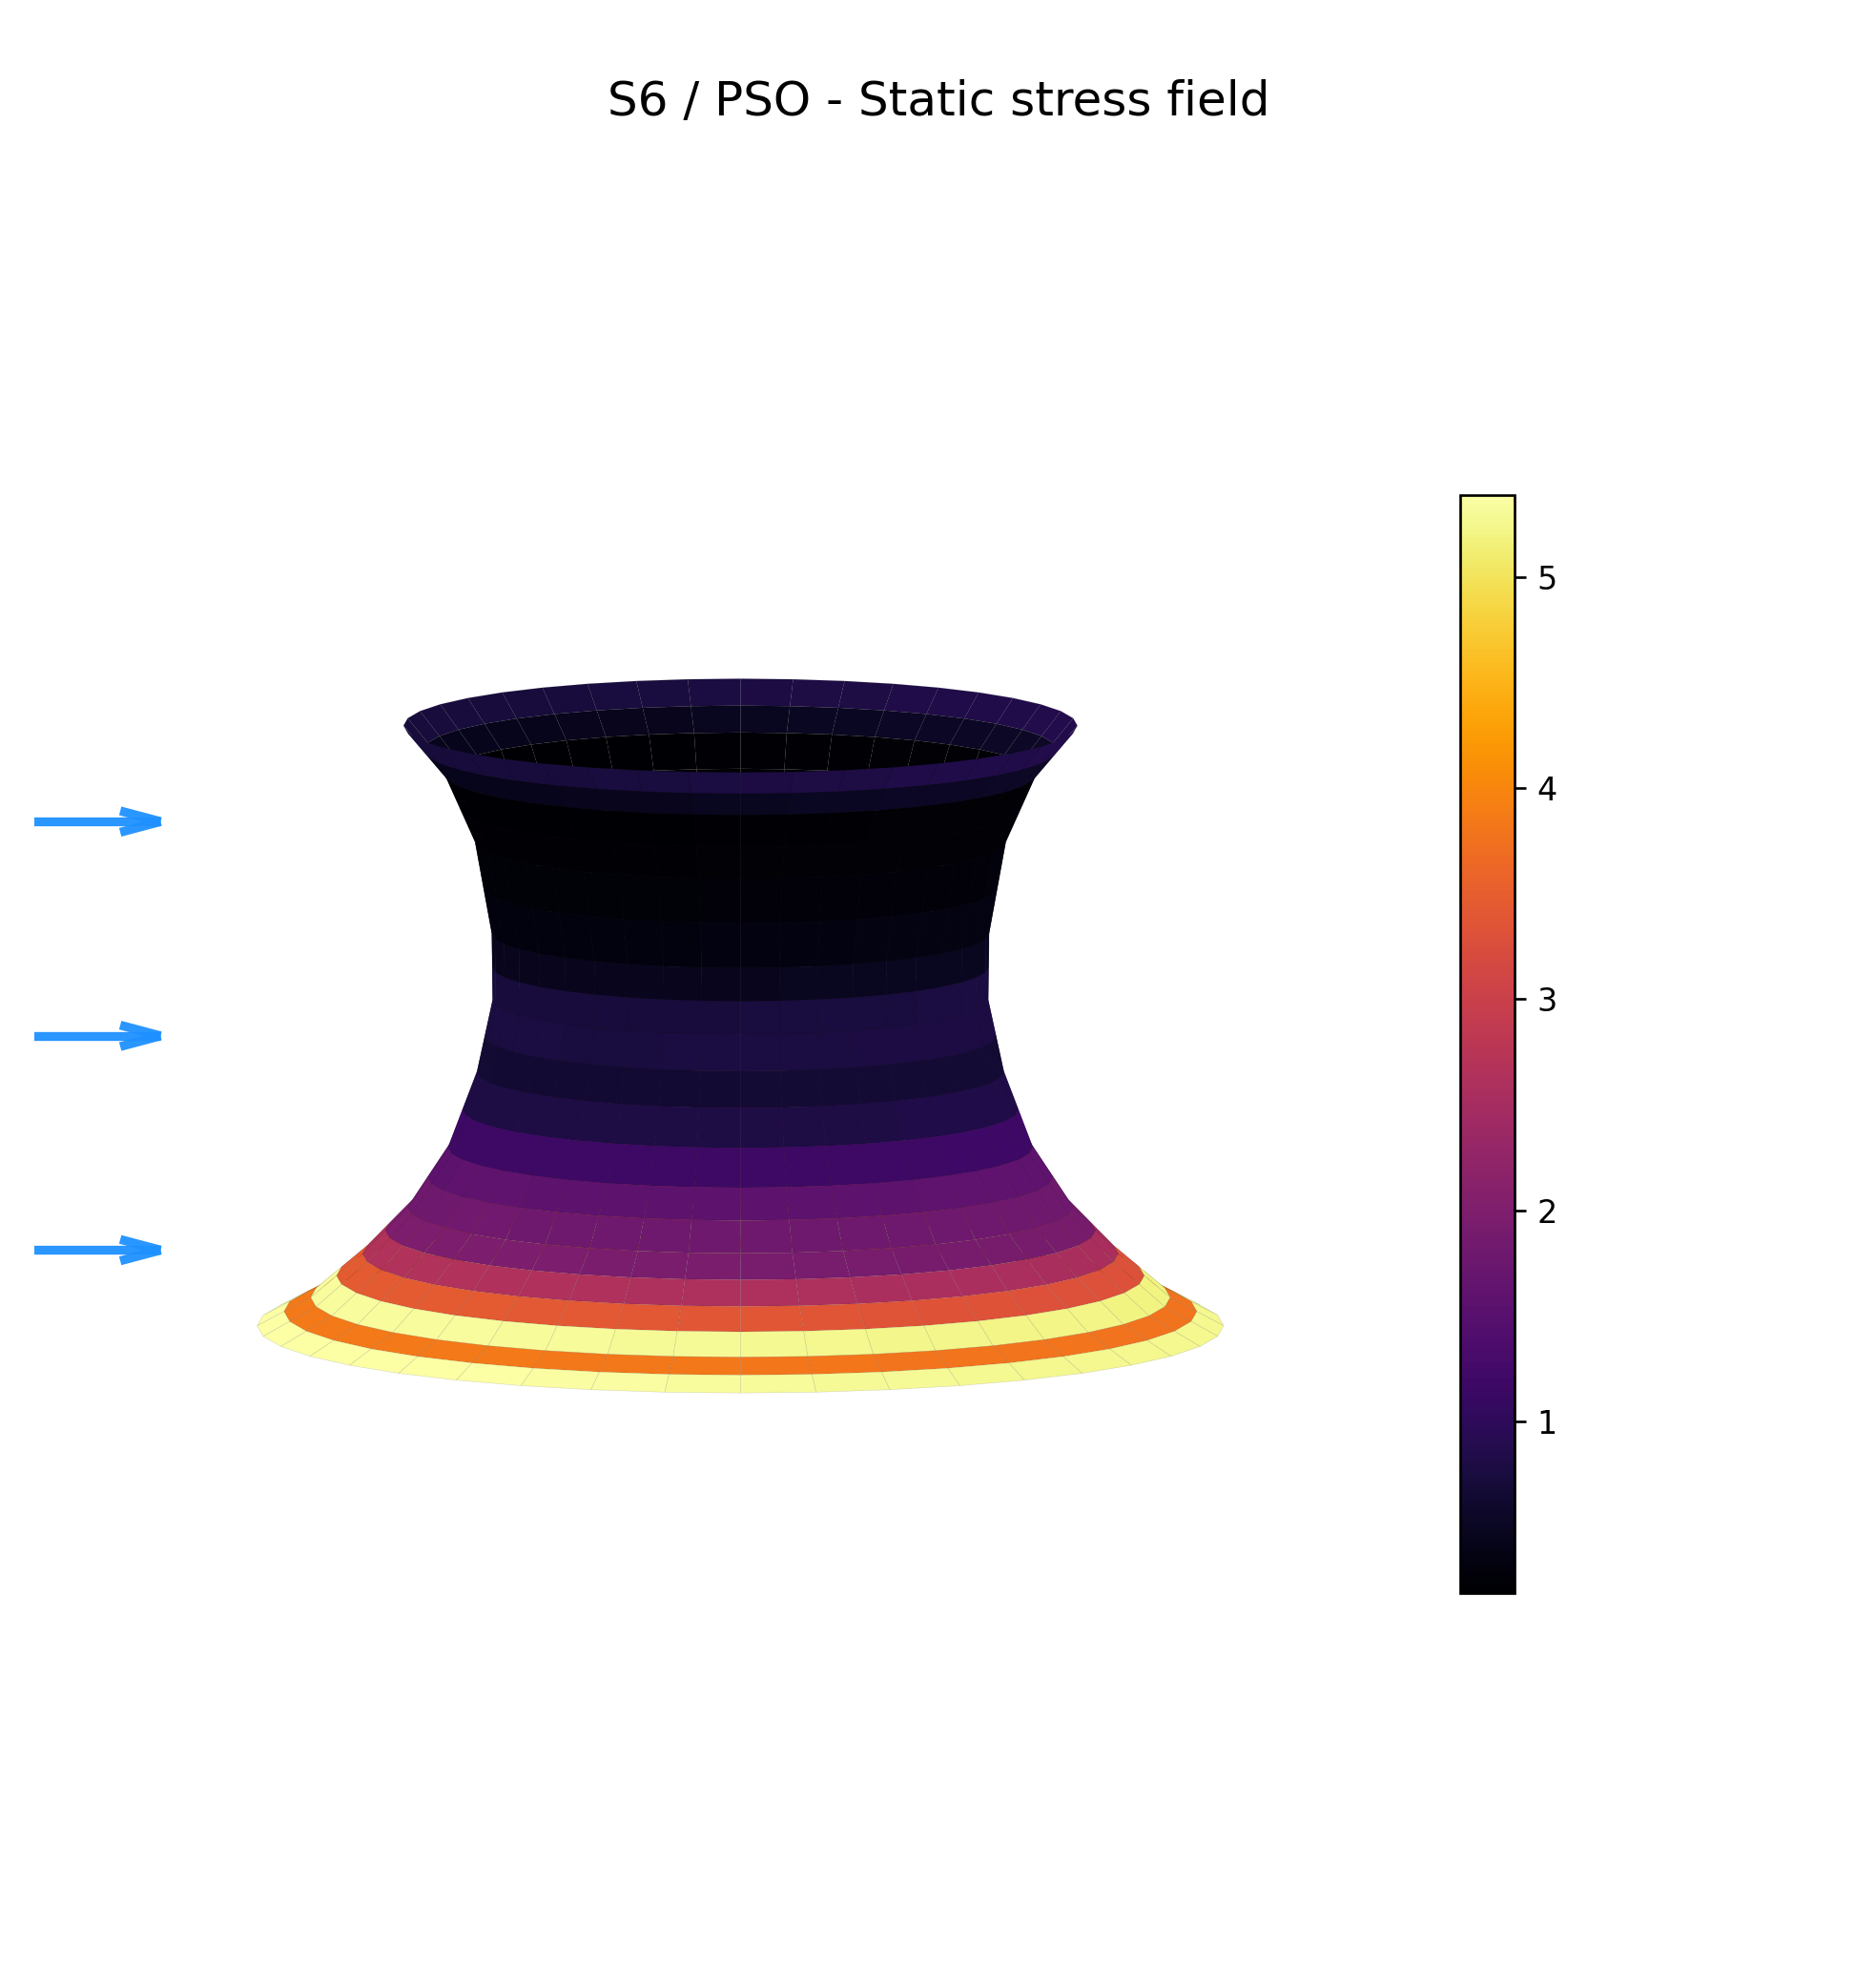
\includegraphics[width=\textwidth]{../results/figures/task7_s6_pso_stress.png}
\caption{S6 / PSO stress}
\end{subfigure}\hfill
\begin{subfigure}{0.32\textwidth}
\centering
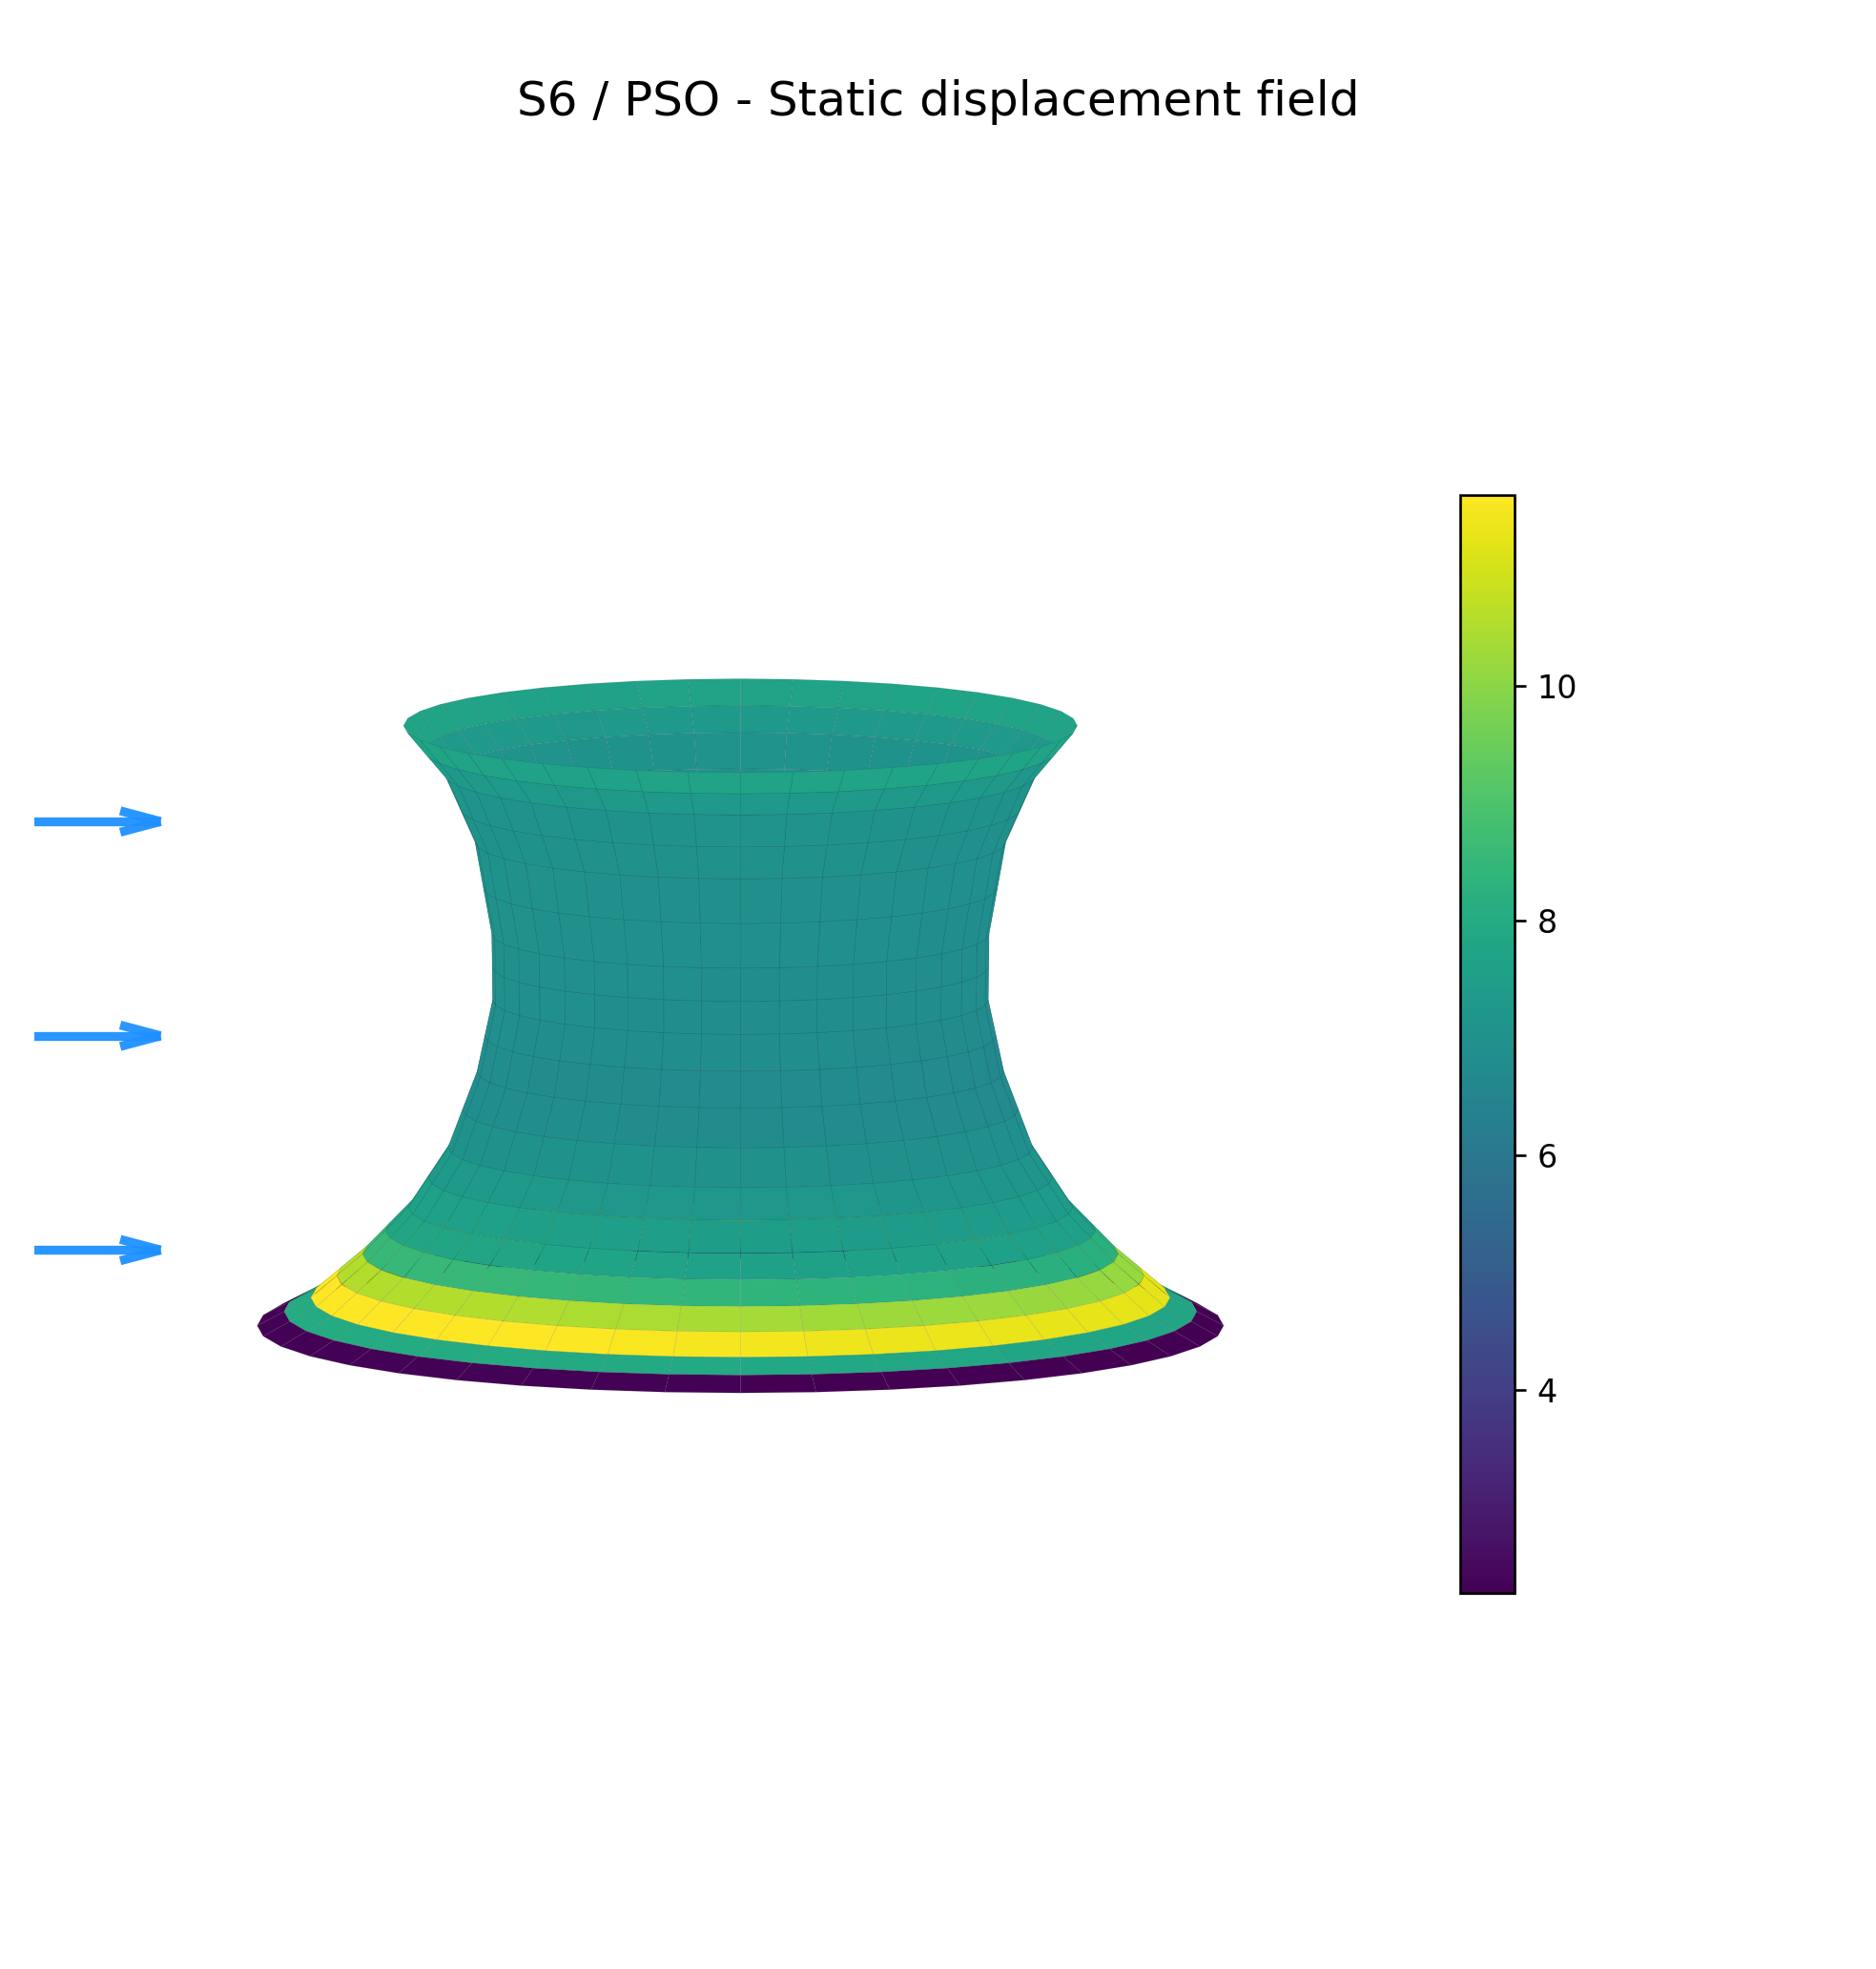
\includegraphics[width=\textwidth]{../results/figures/task7_s6_pso_displacement.png}
\caption{S6 / PSO displacement}
\end{subfigure}\hfill
\begin{subfigure}{0.32\textwidth}
\centering
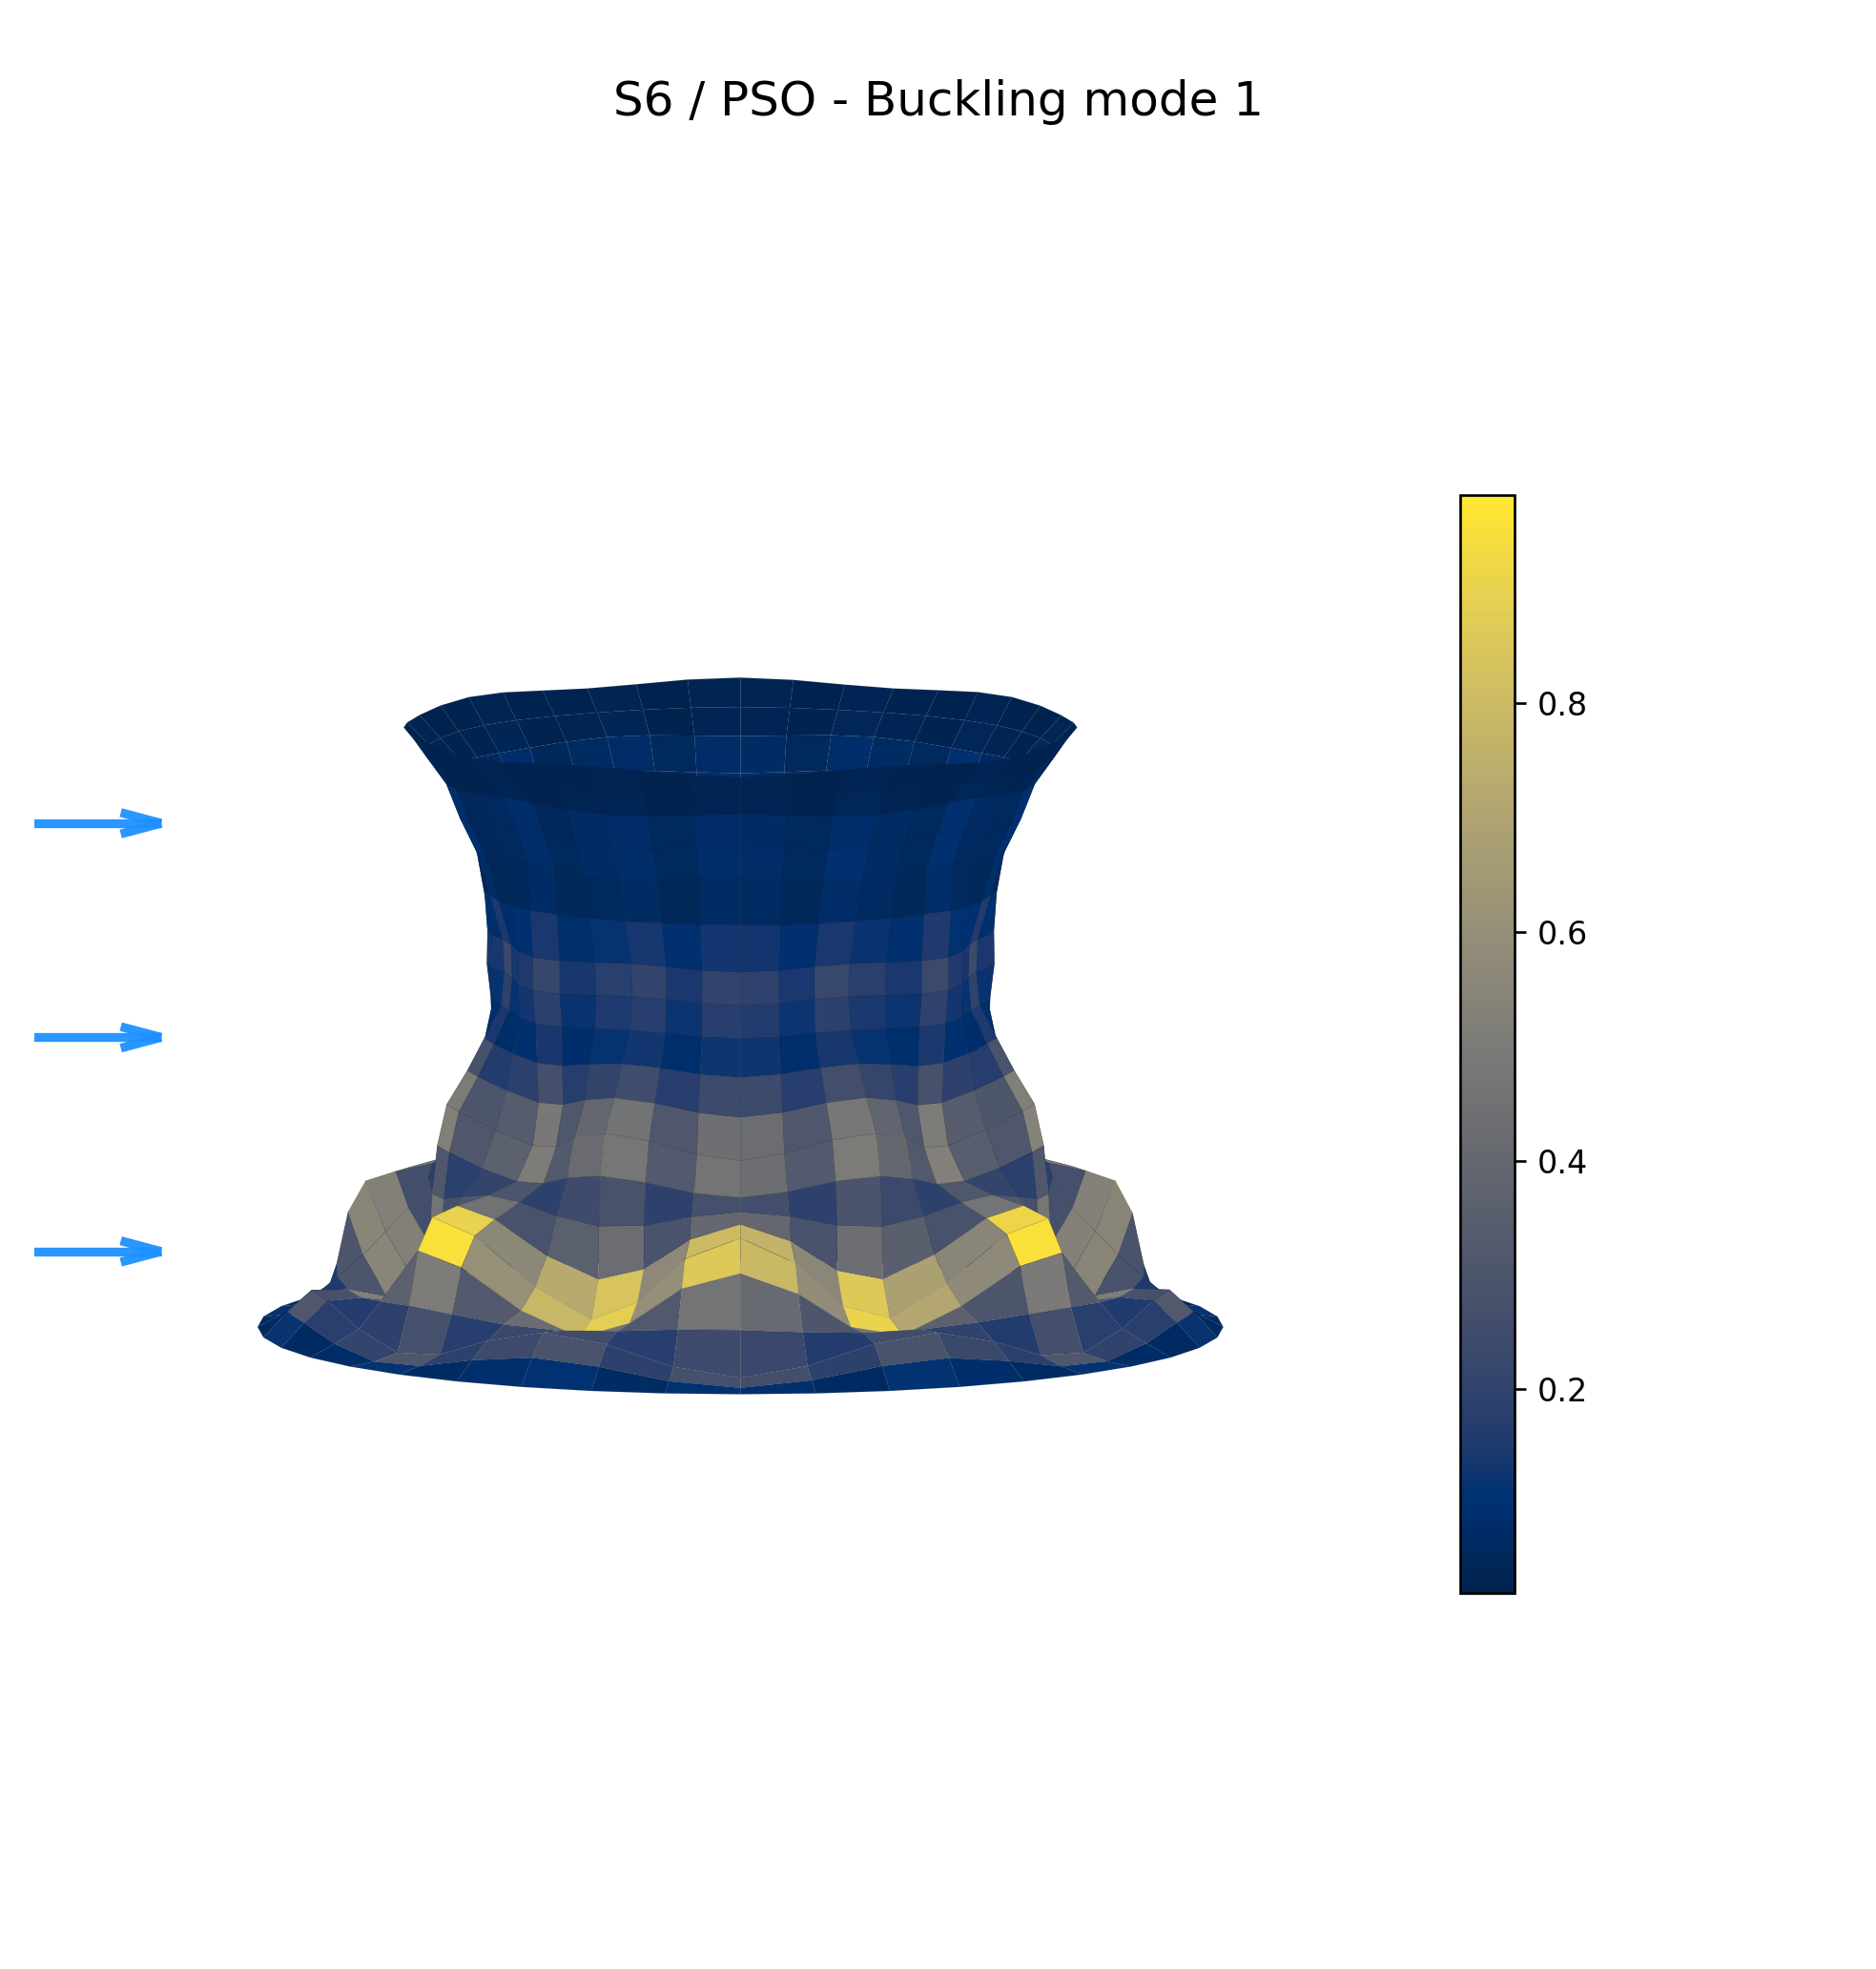
\includegraphics[width=\textwidth]{../results/figures/task7_s6_pso_buckling_mode1.png}
\caption{S6 / PSO buckling}
\end{subfigure}
\caption{Combined visual fields}
\end{figure}


\subsection{S6 / SA}


\begin{figure}[H]
\centering
\begin{subfigure}{0.32\textwidth}
\centering
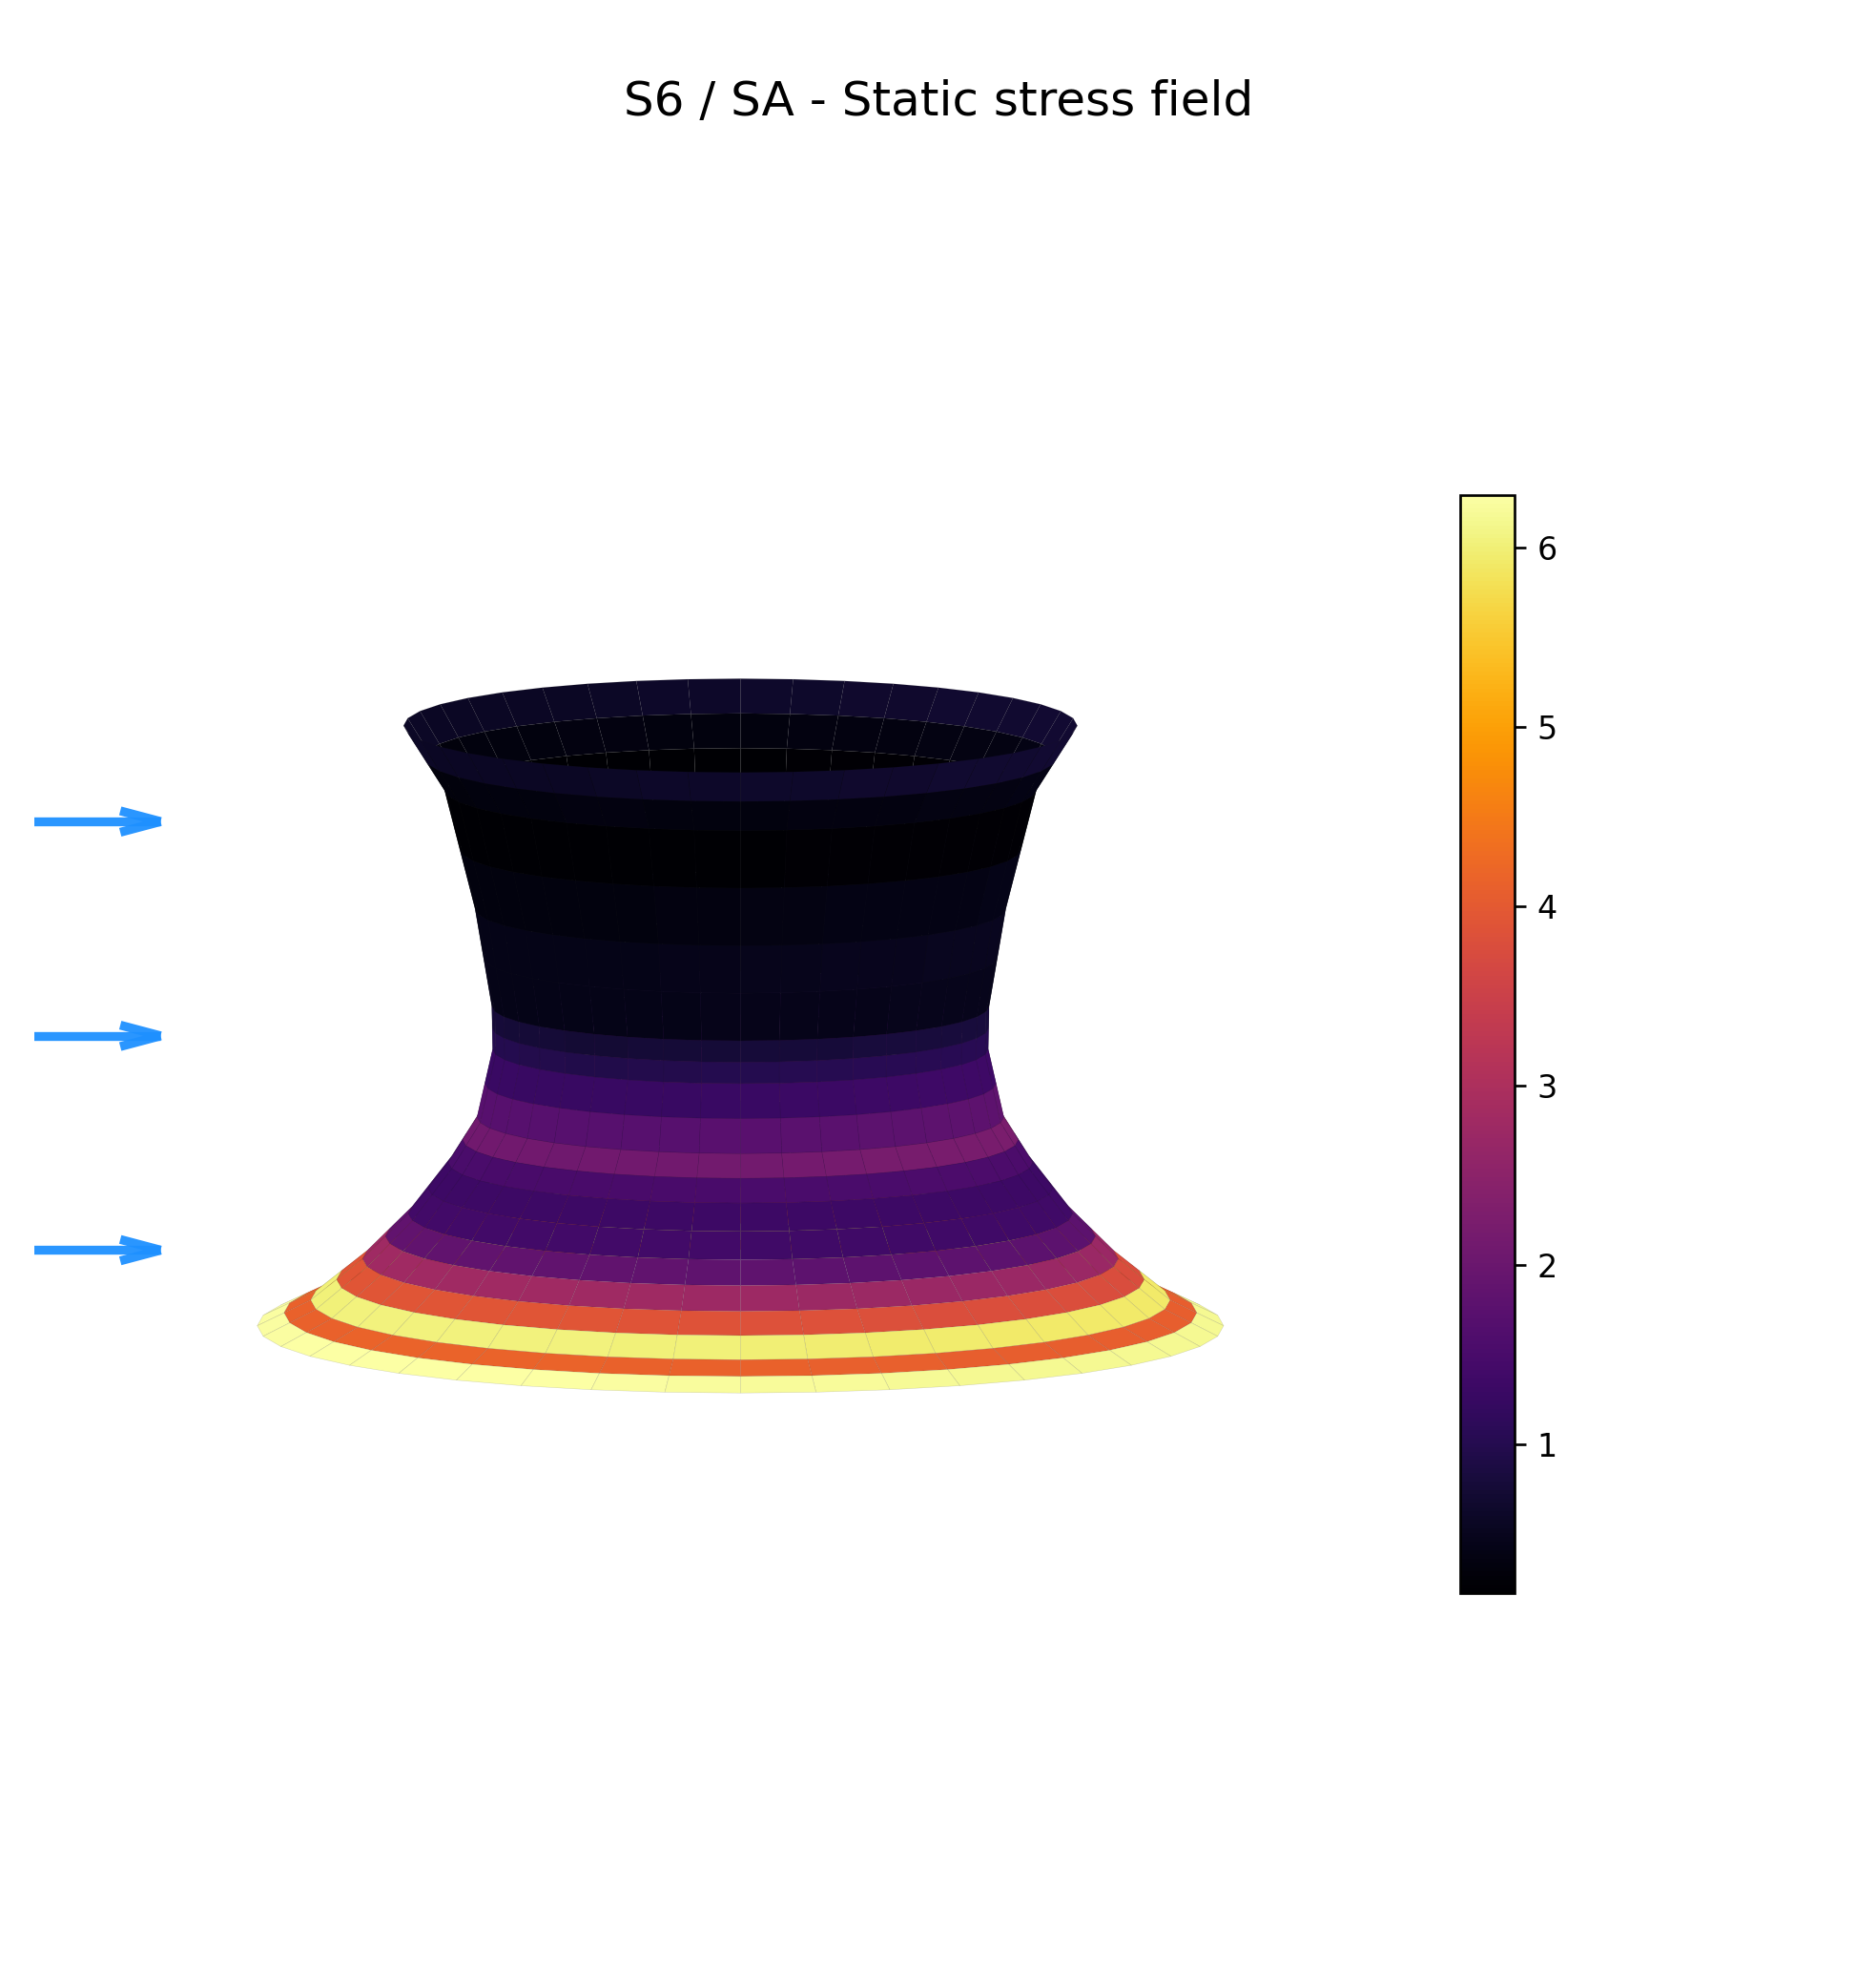
\includegraphics[width=\textwidth]{../results/figures/task7_s6_sa_stress.png}
\caption{S6 / SA stress}
\end{subfigure}\hfill
\begin{subfigure}{0.32\textwidth}
\centering
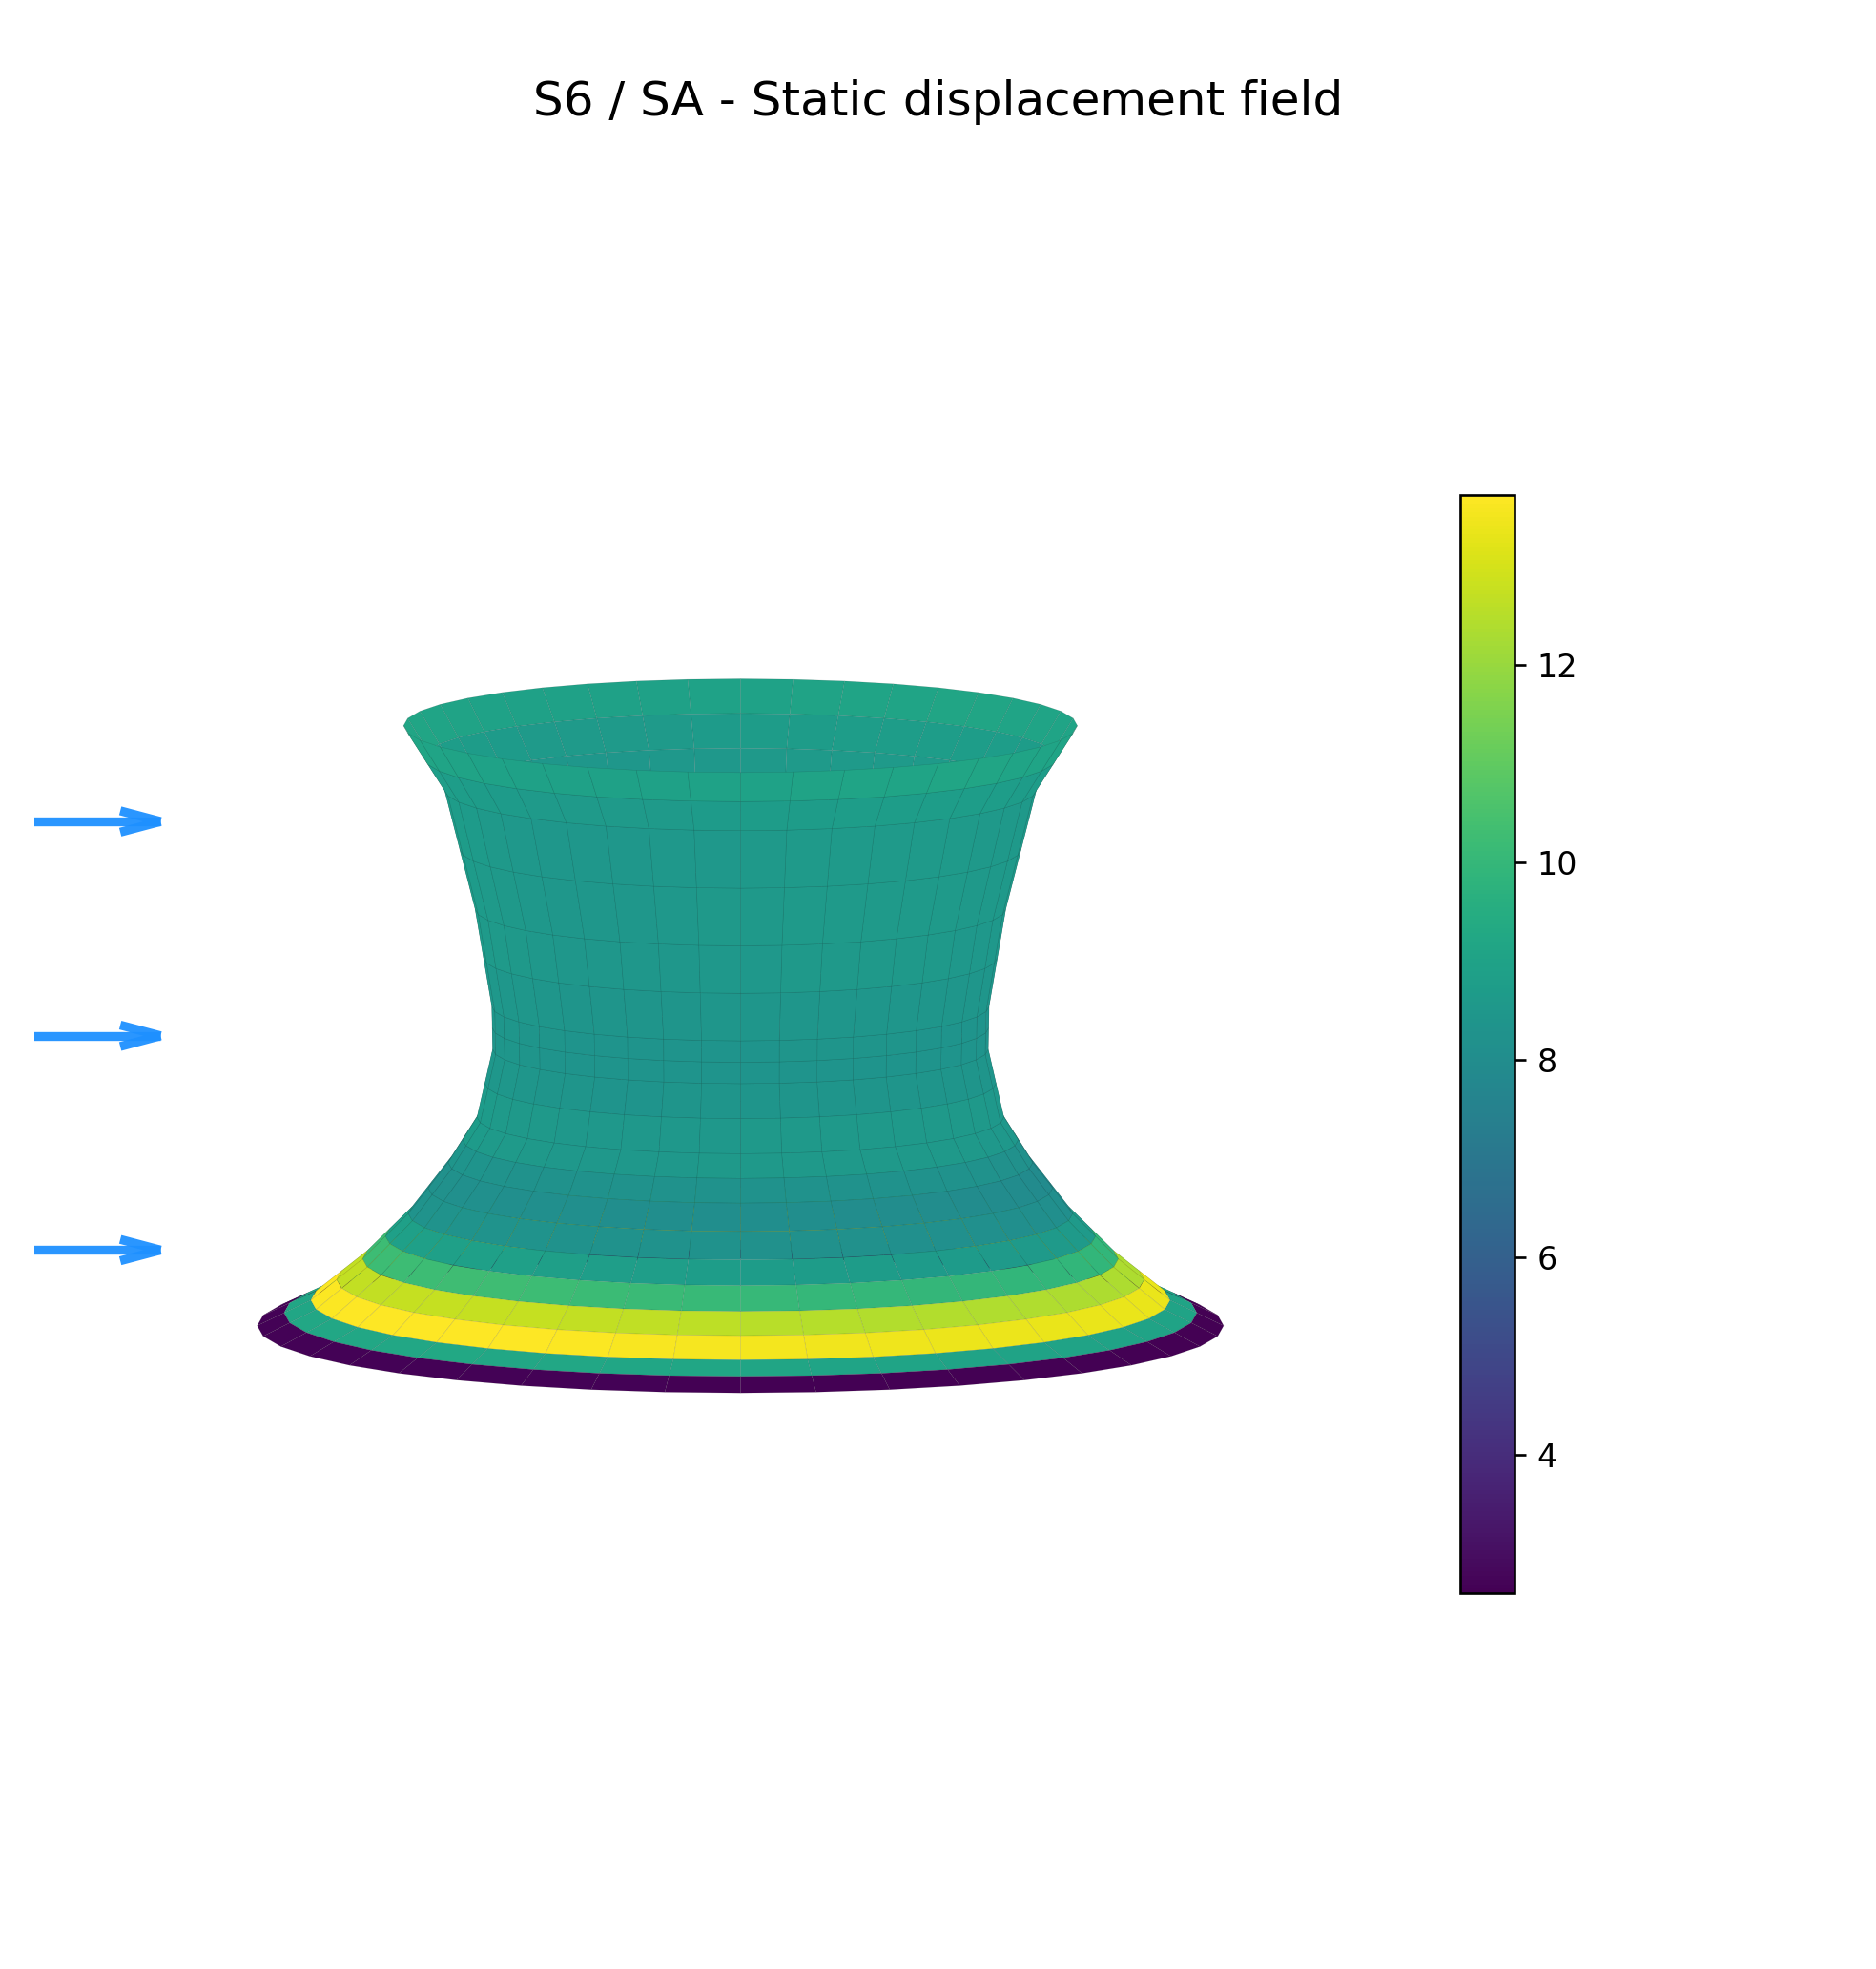
\includegraphics[width=\textwidth]{../results/figures/task7_s6_sa_displacement.png}
\caption{S6 / SA displacement}
\end{subfigure}\hfill
\begin{subfigure}{0.32\textwidth}
\centering
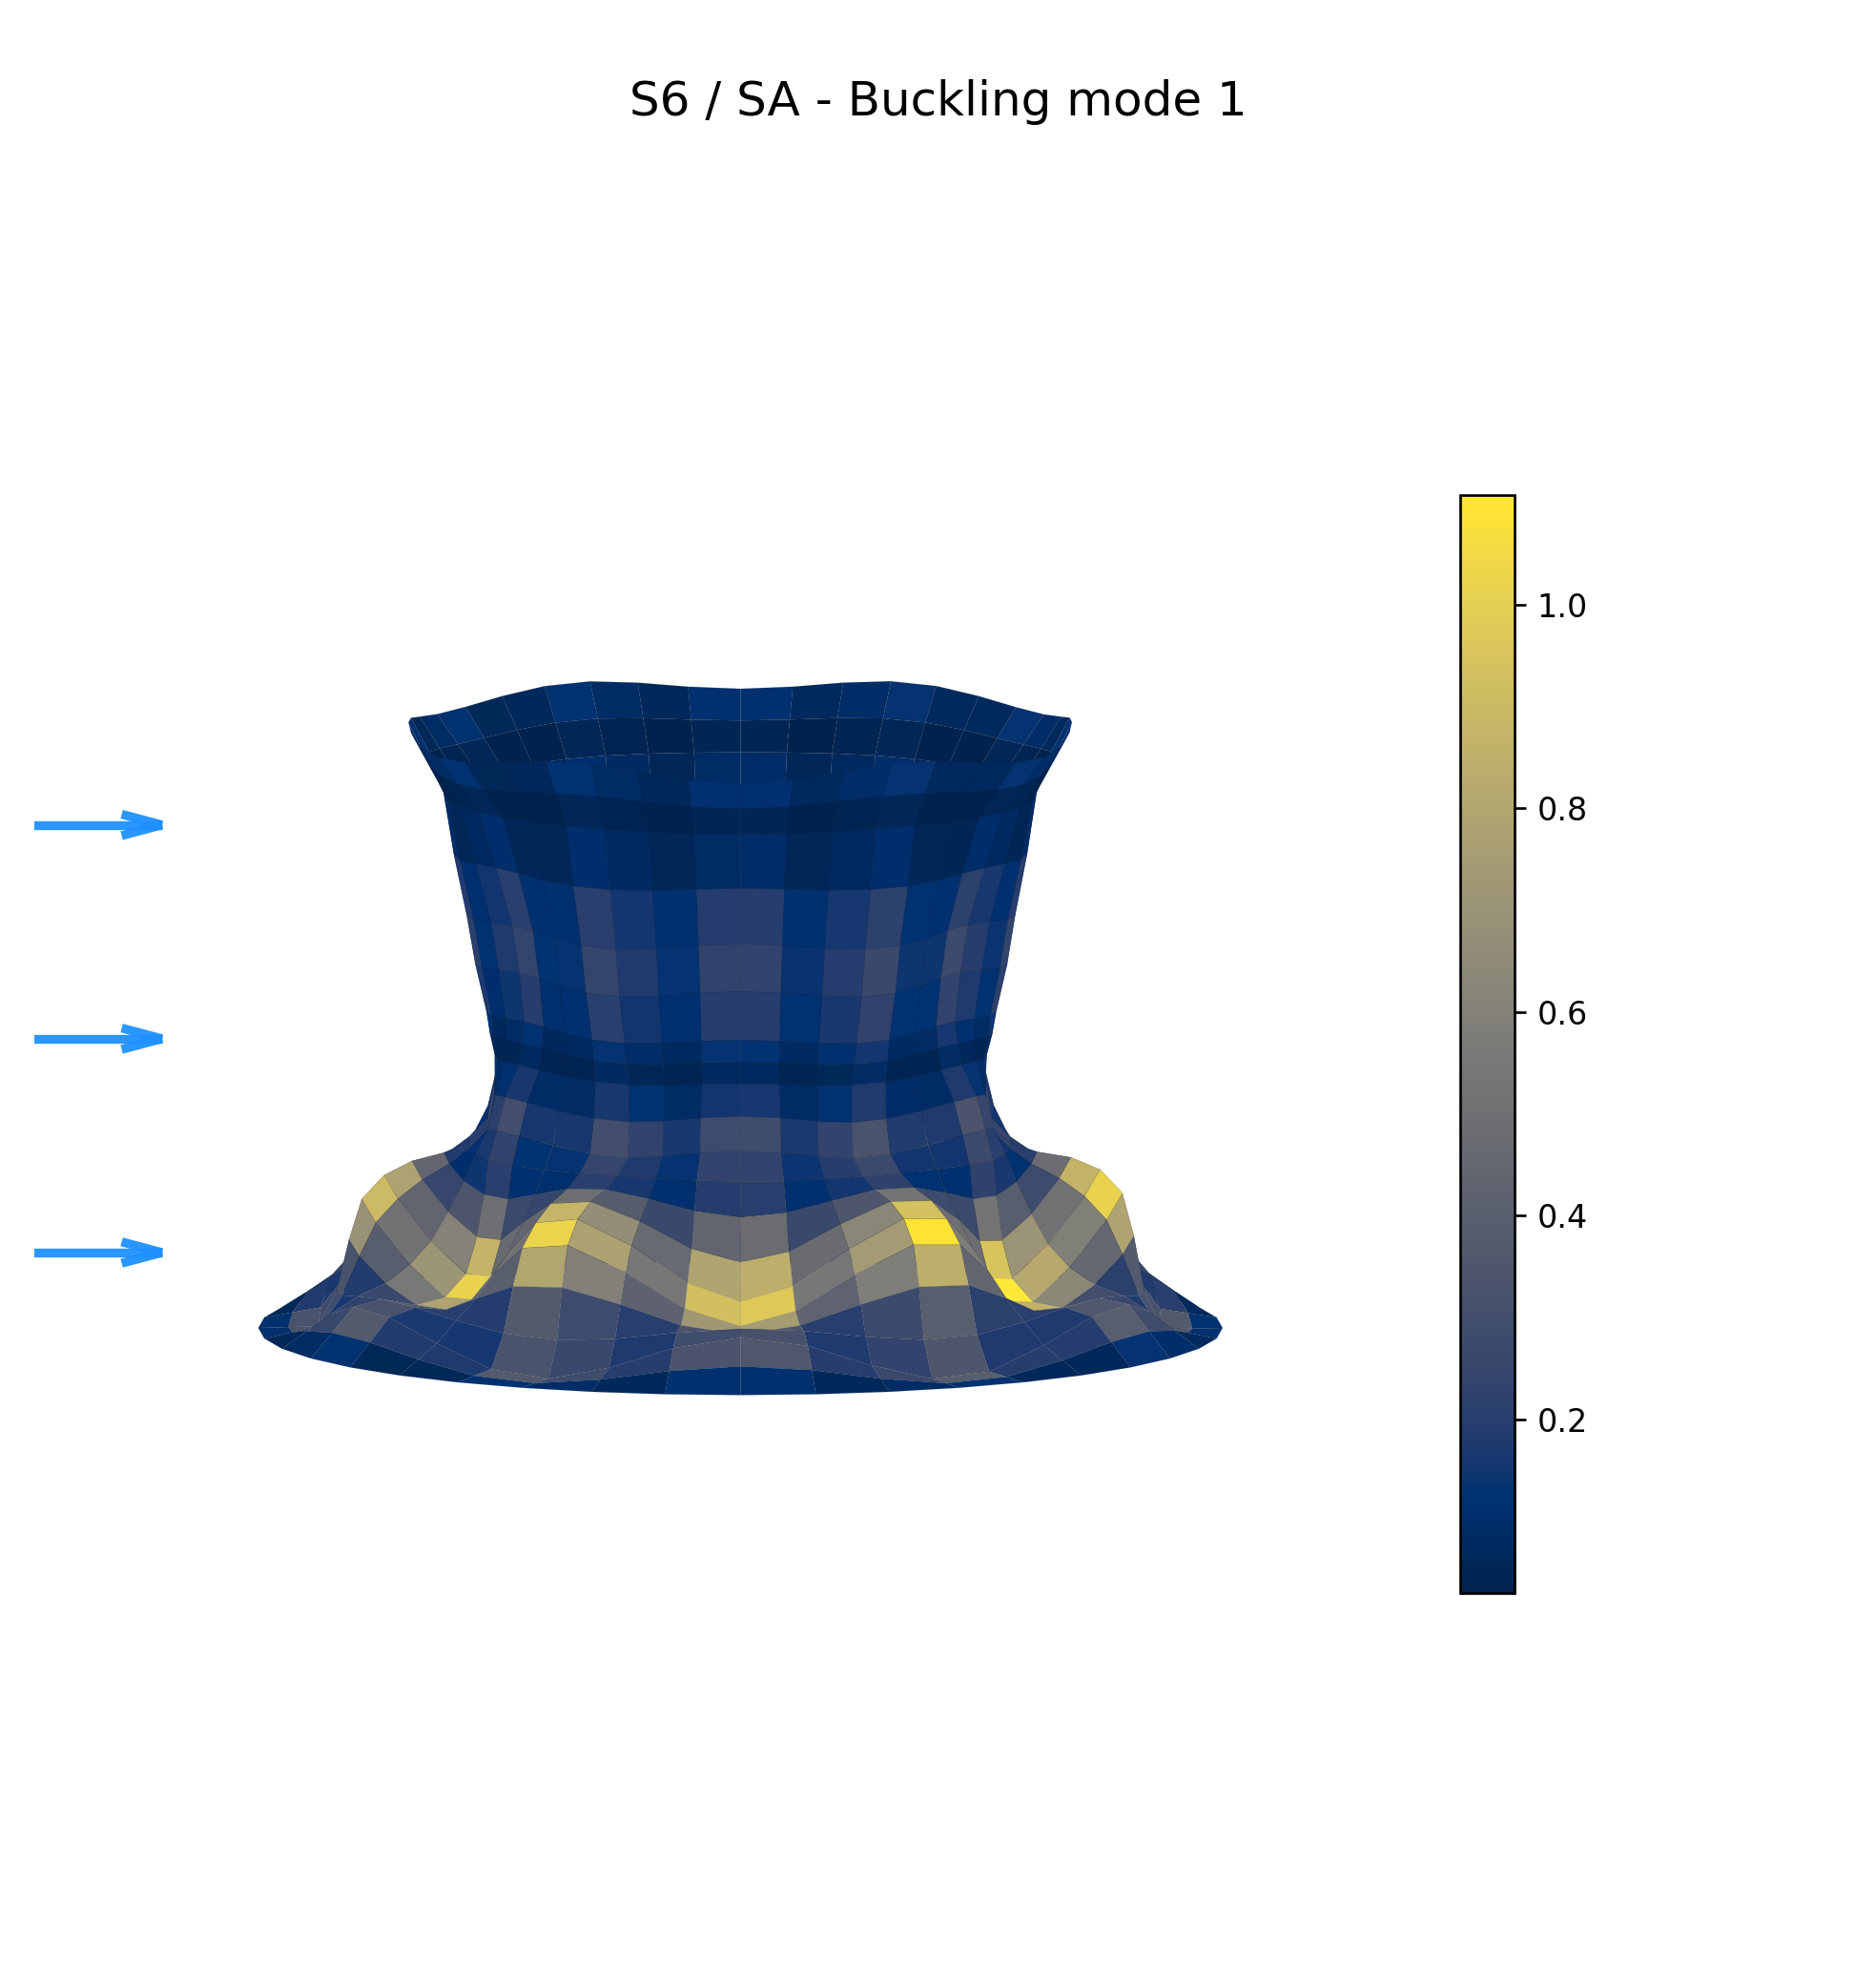
\includegraphics[width=\textwidth]{../results/figures/task7_s6_sa_buckling_mode1.png}
\caption{S6 / SA buckling}
\end{subfigure}
\caption{Combined visual fields}
\end{figure}


\section{Scenario S7}


\subsection{S7 / PSO}


\begin{figure}[H]
\centering
\begin{subfigure}{0.32\textwidth}
\centering
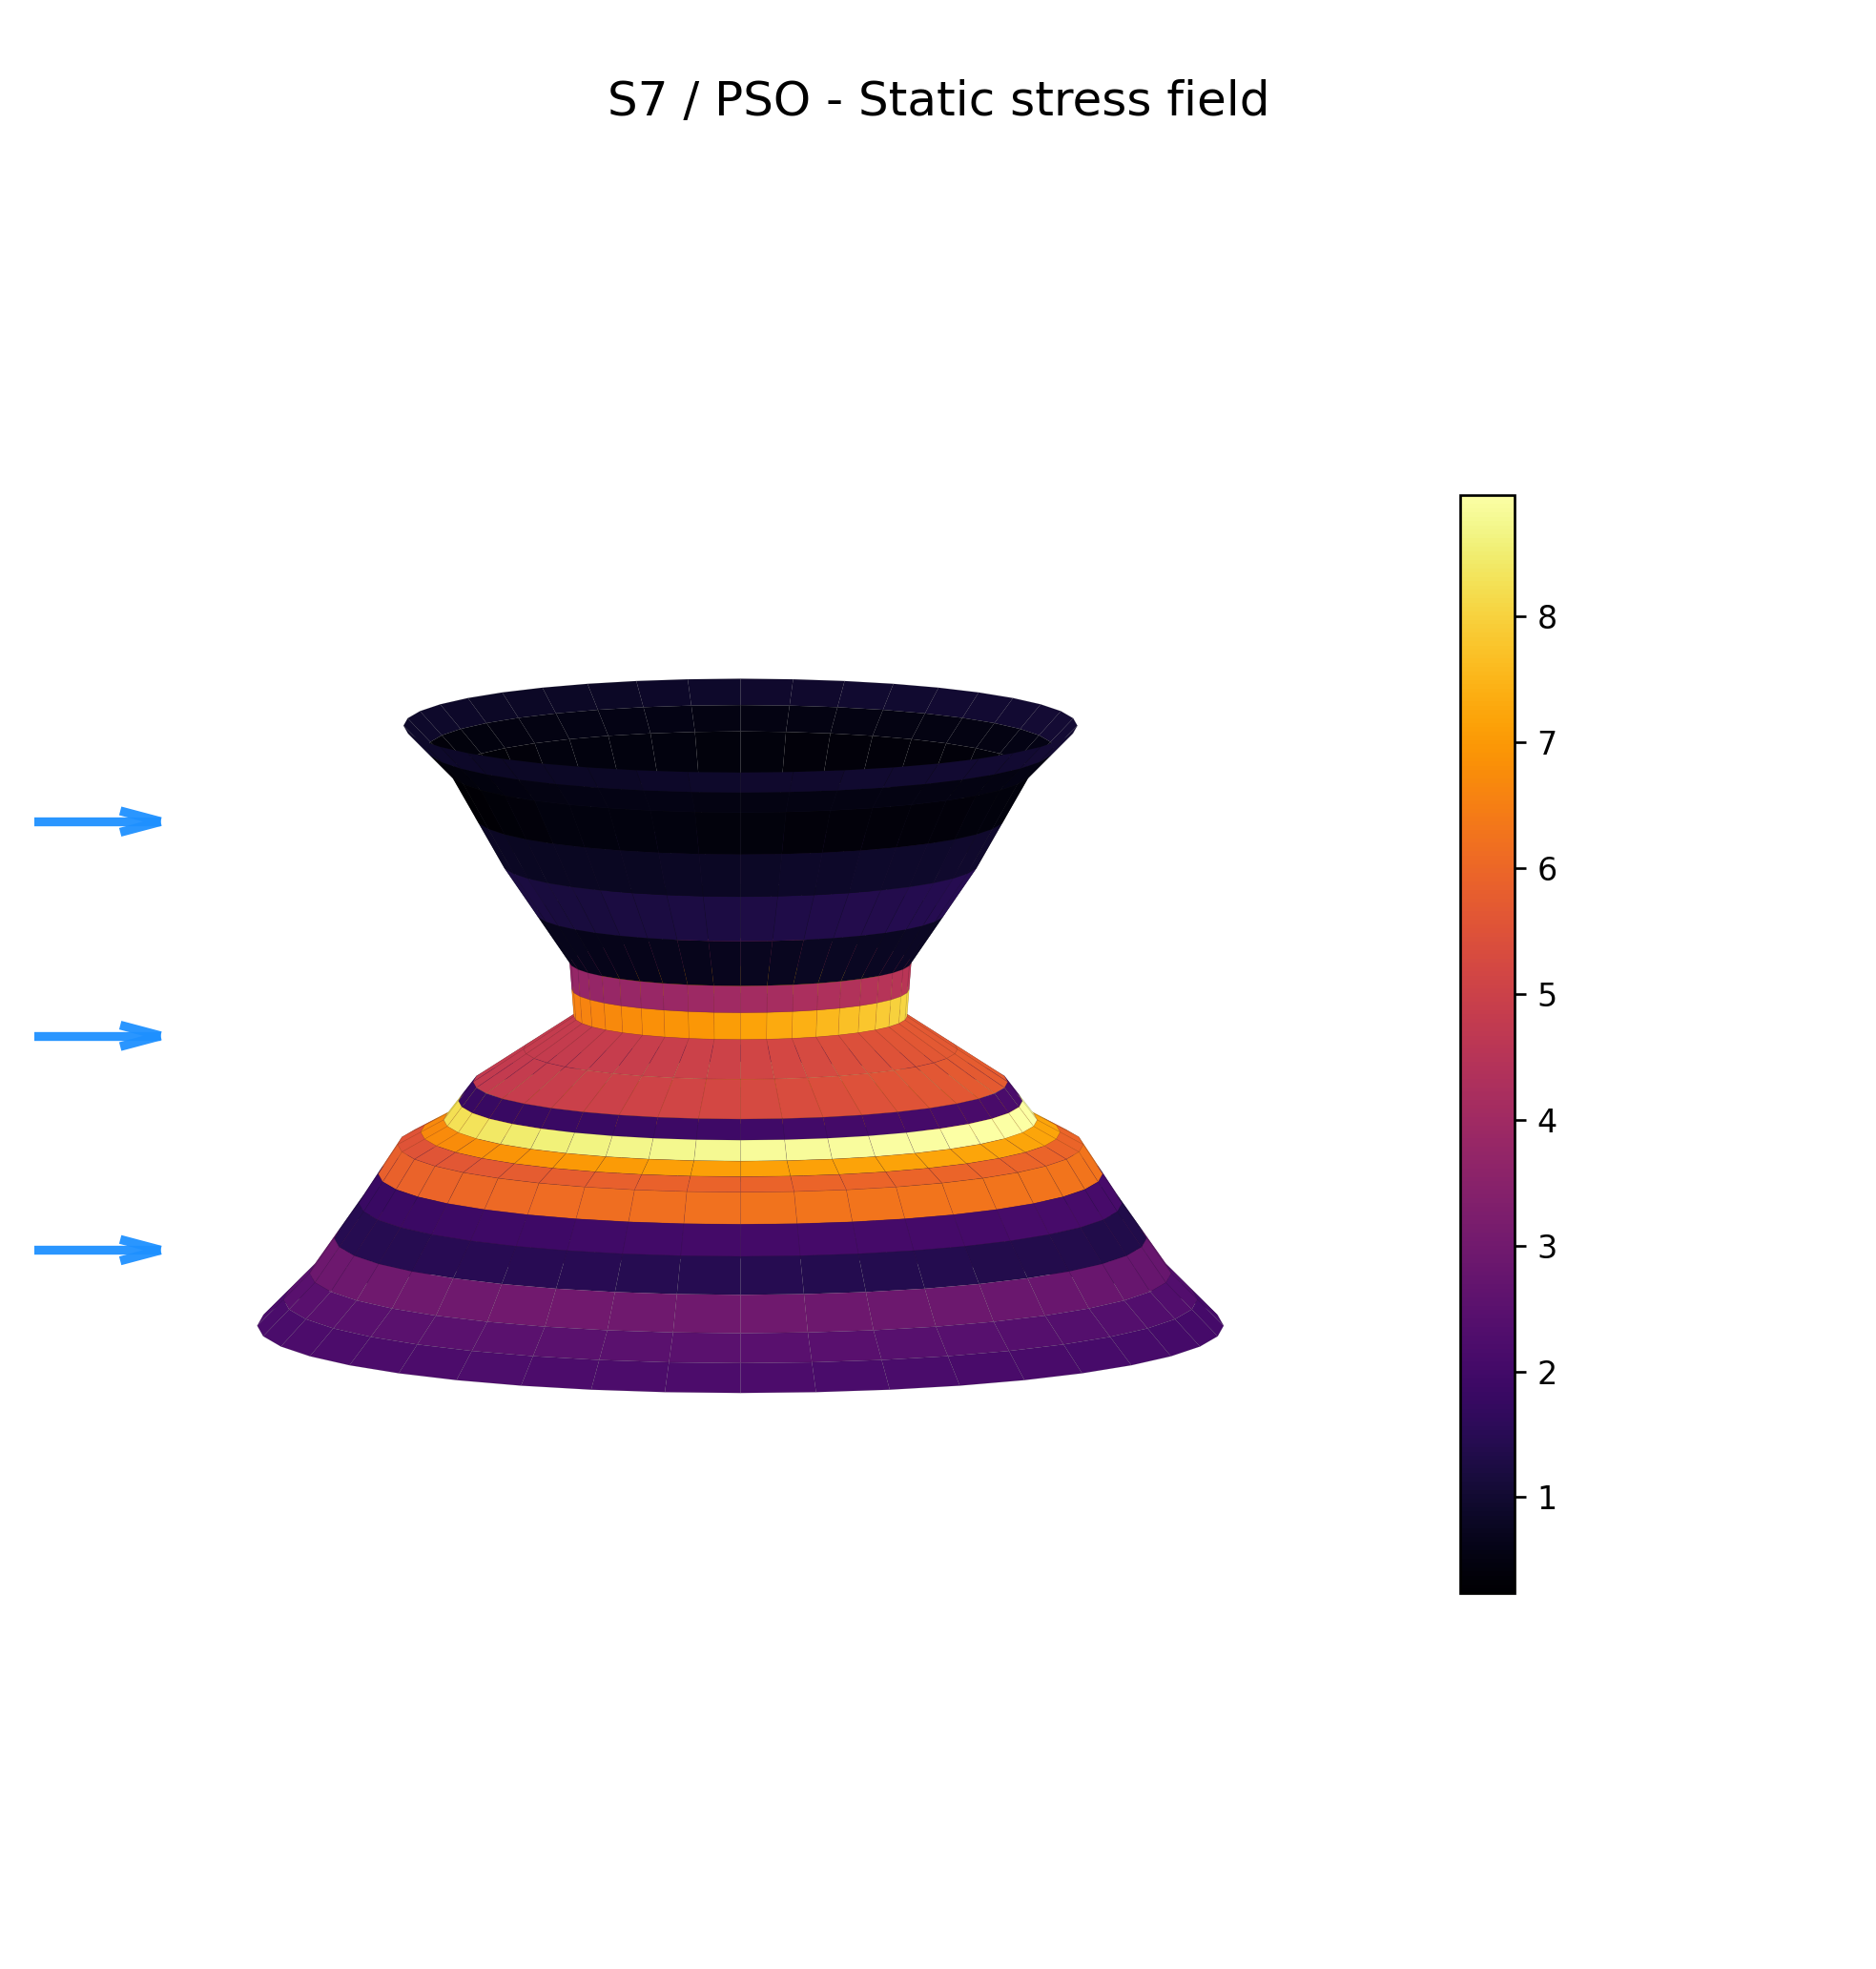
\includegraphics[width=\textwidth]{../results/figures/task7_s7_pso_stress.png}
\caption{S7 / PSO stress}
\end{subfigure}\hfill
\begin{subfigure}{0.32\textwidth}
\centering
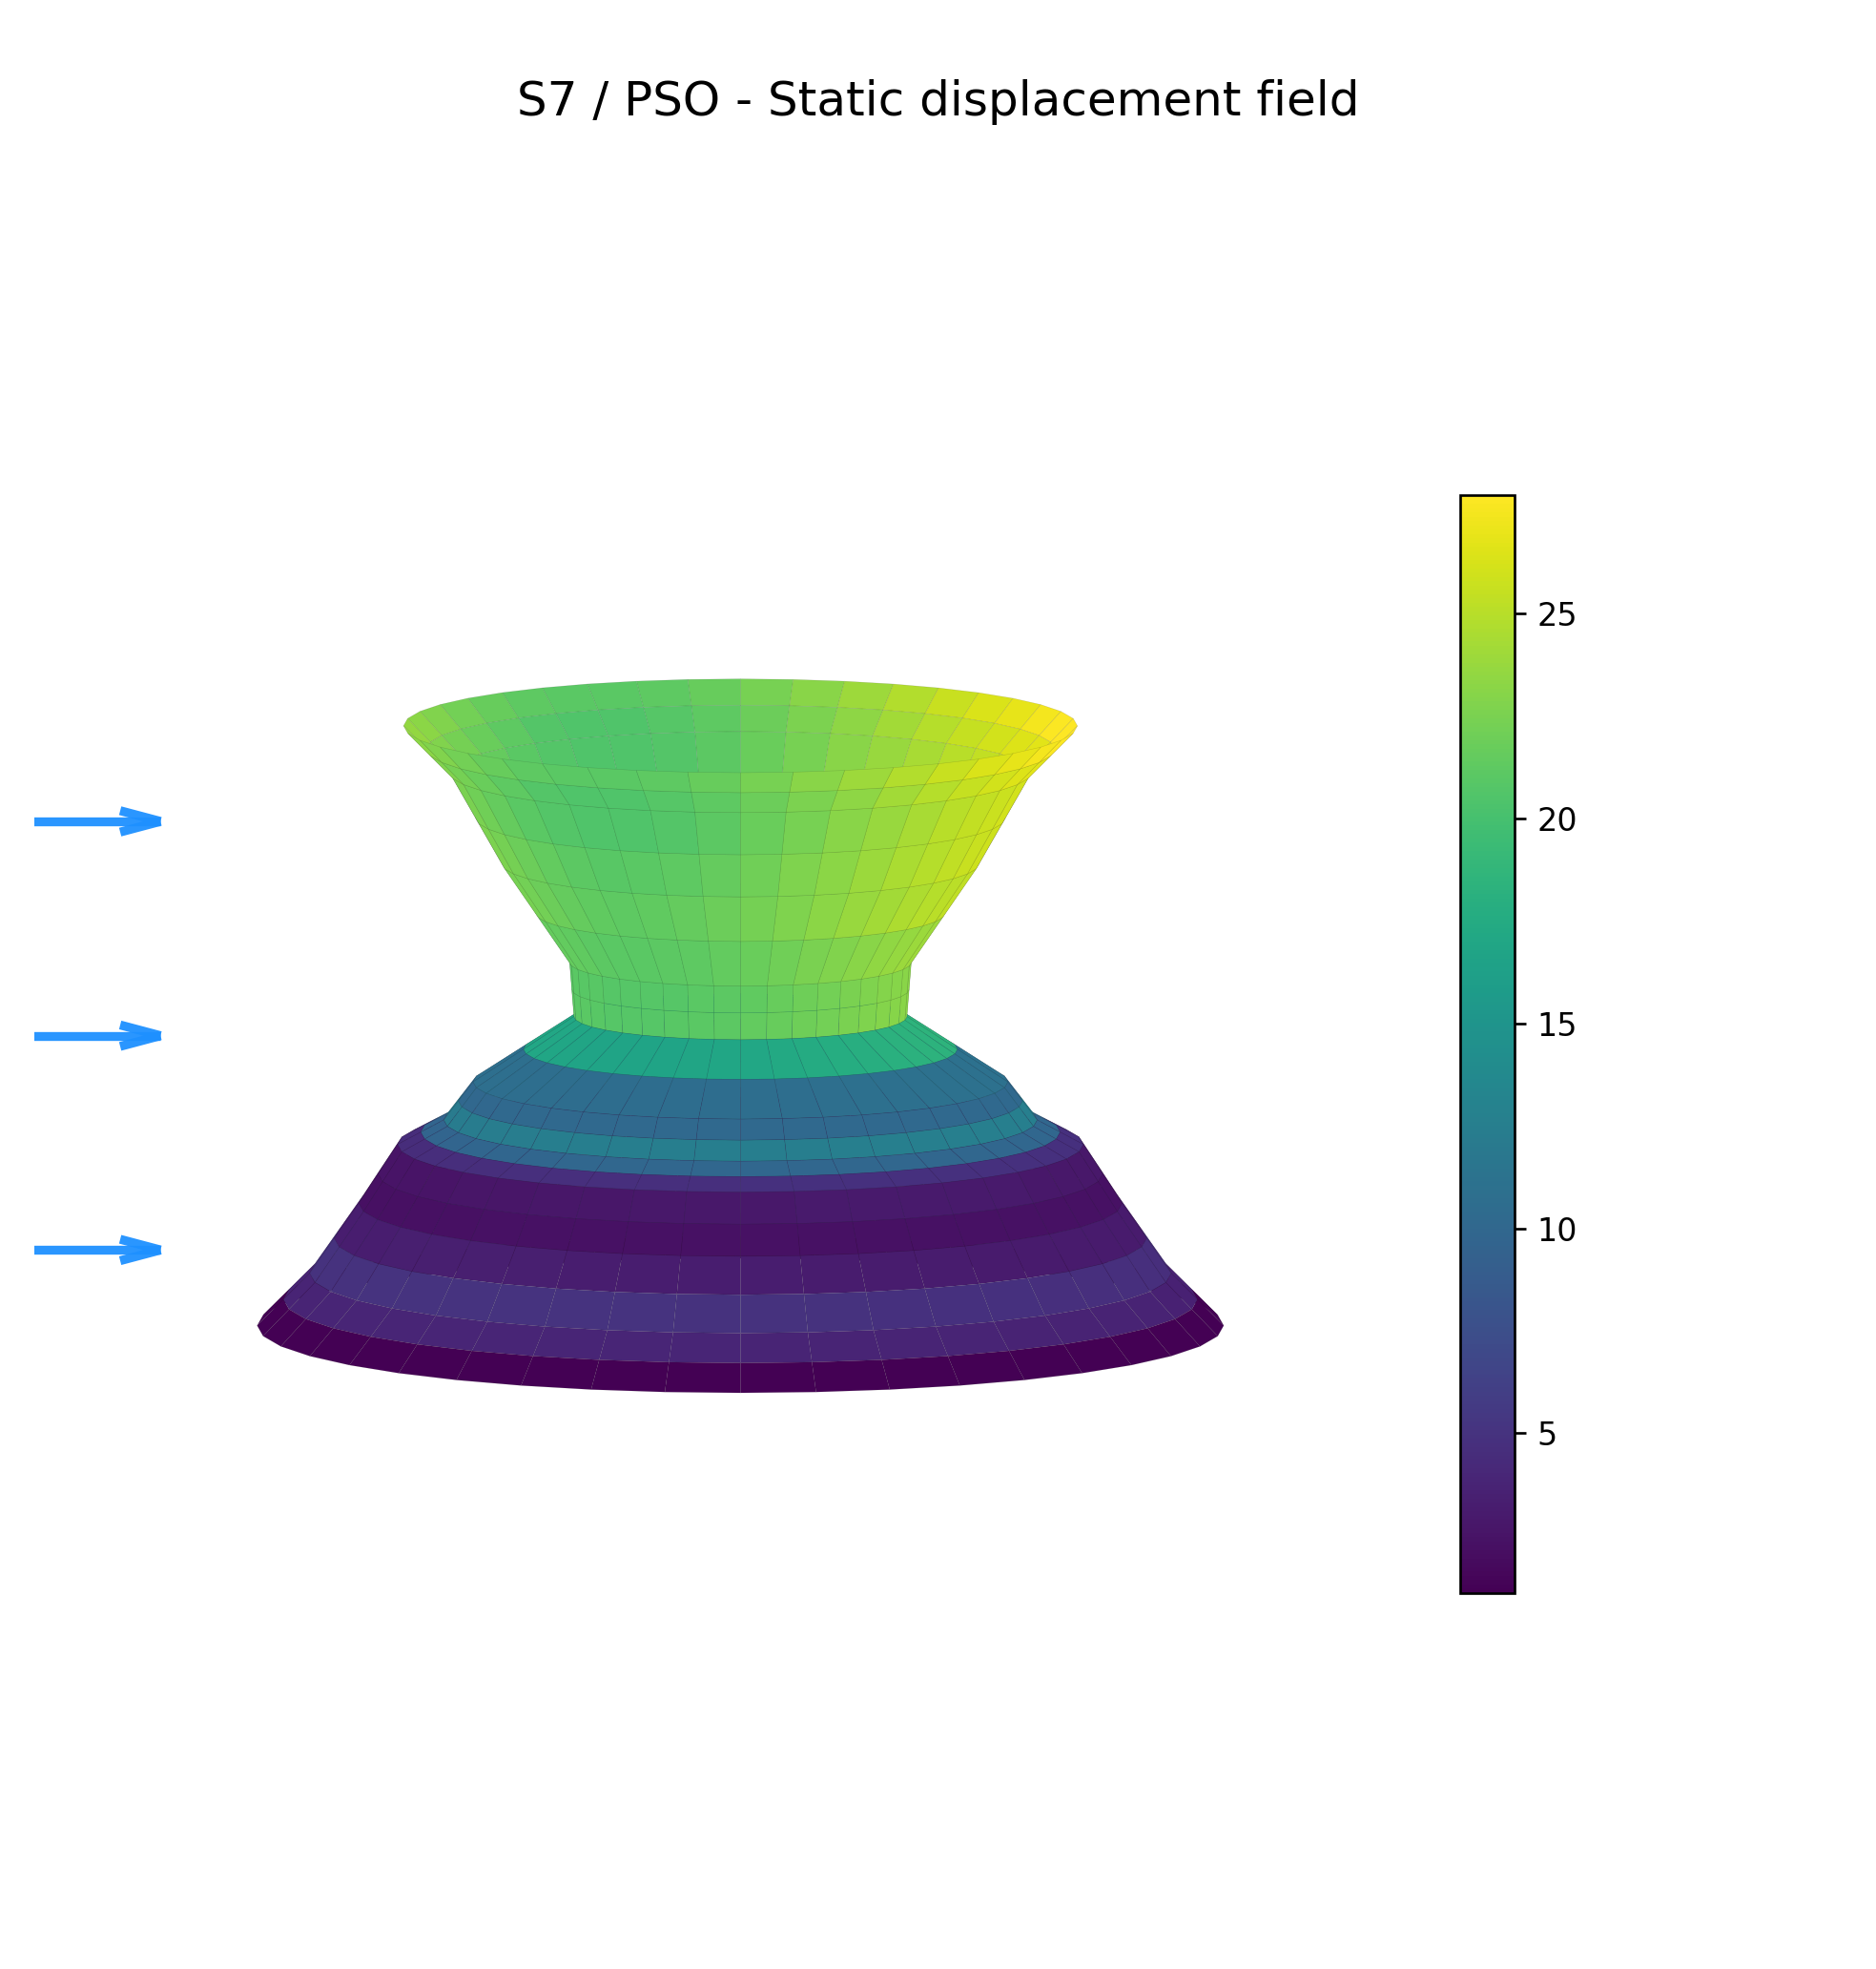
\includegraphics[width=\textwidth]{../results/figures/task7_s7_pso_displacement.png}
\caption{S7 / PSO displacement}
\end{subfigure}\hfill
\begin{subfigure}{0.32\textwidth}
\centering
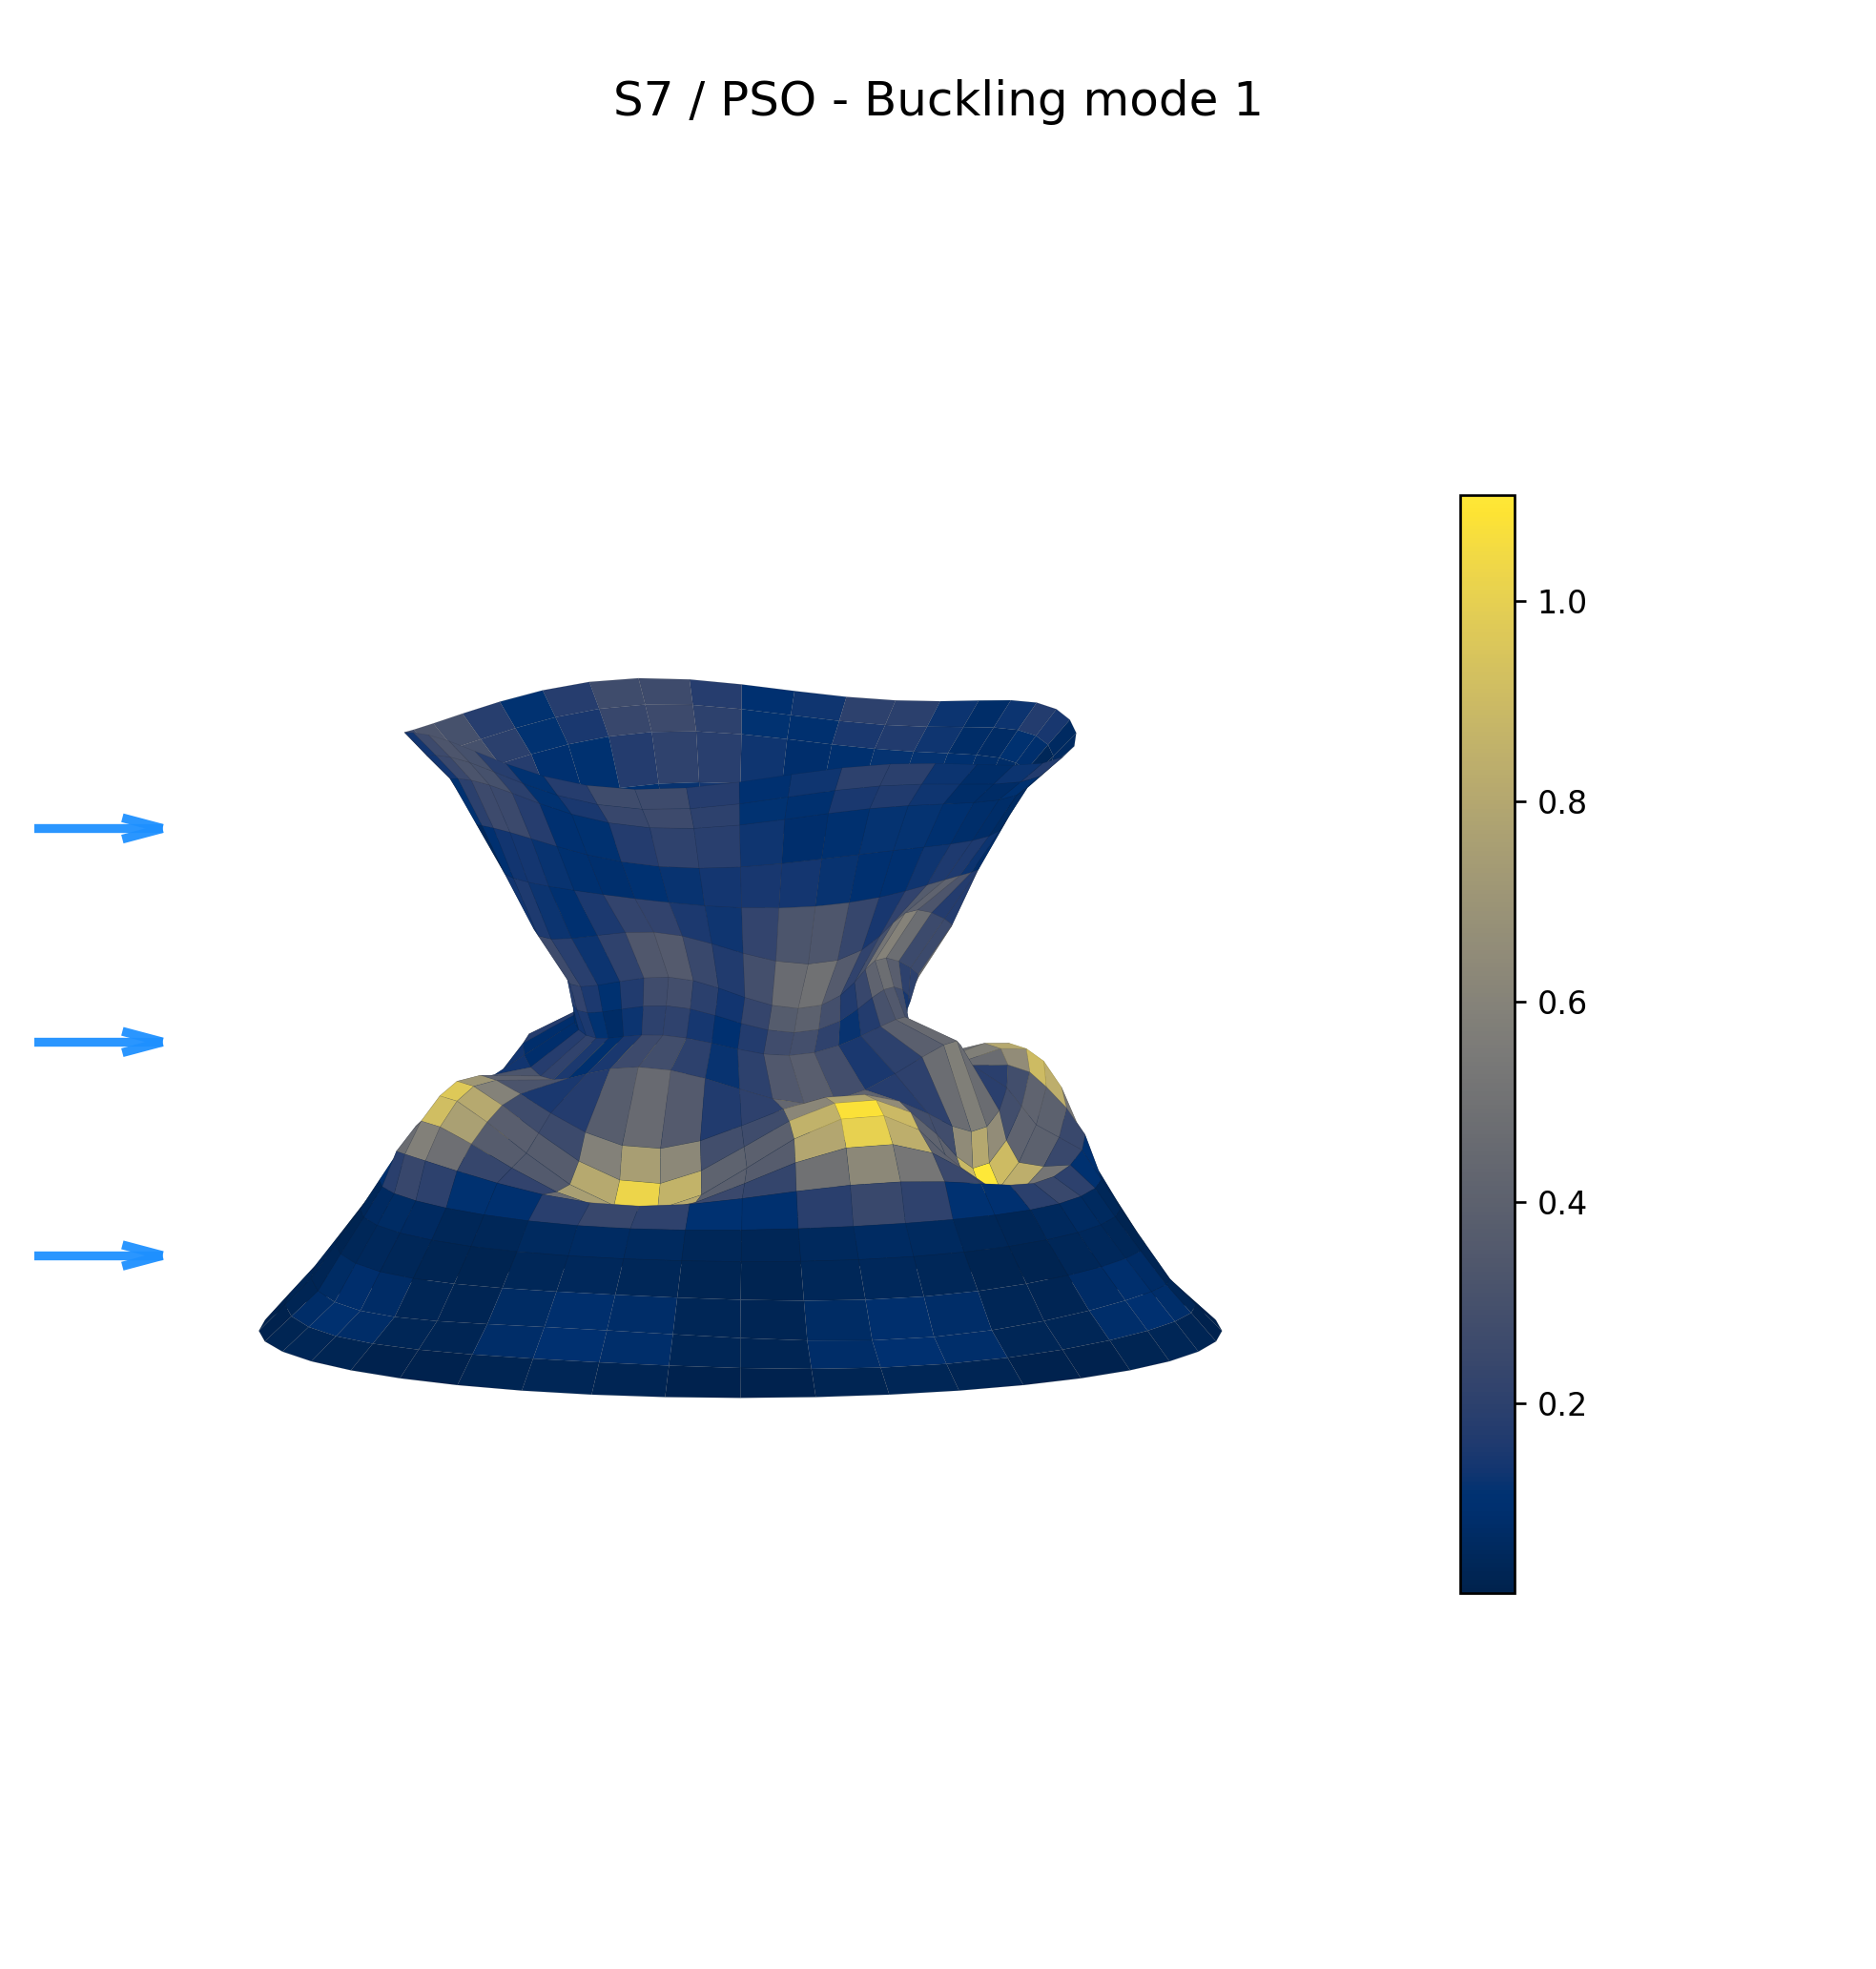
\includegraphics[width=\textwidth]{../results/figures/task7_s7_pso_buckling_mode1.png}
\caption{S7 / PSO buckling}
\end{subfigure}
\caption{Combined visual fields}
\end{figure}


\subsection{S7 / SA}


\begin{figure}[H]
\centering
\begin{subfigure}{0.32\textwidth}
\centering
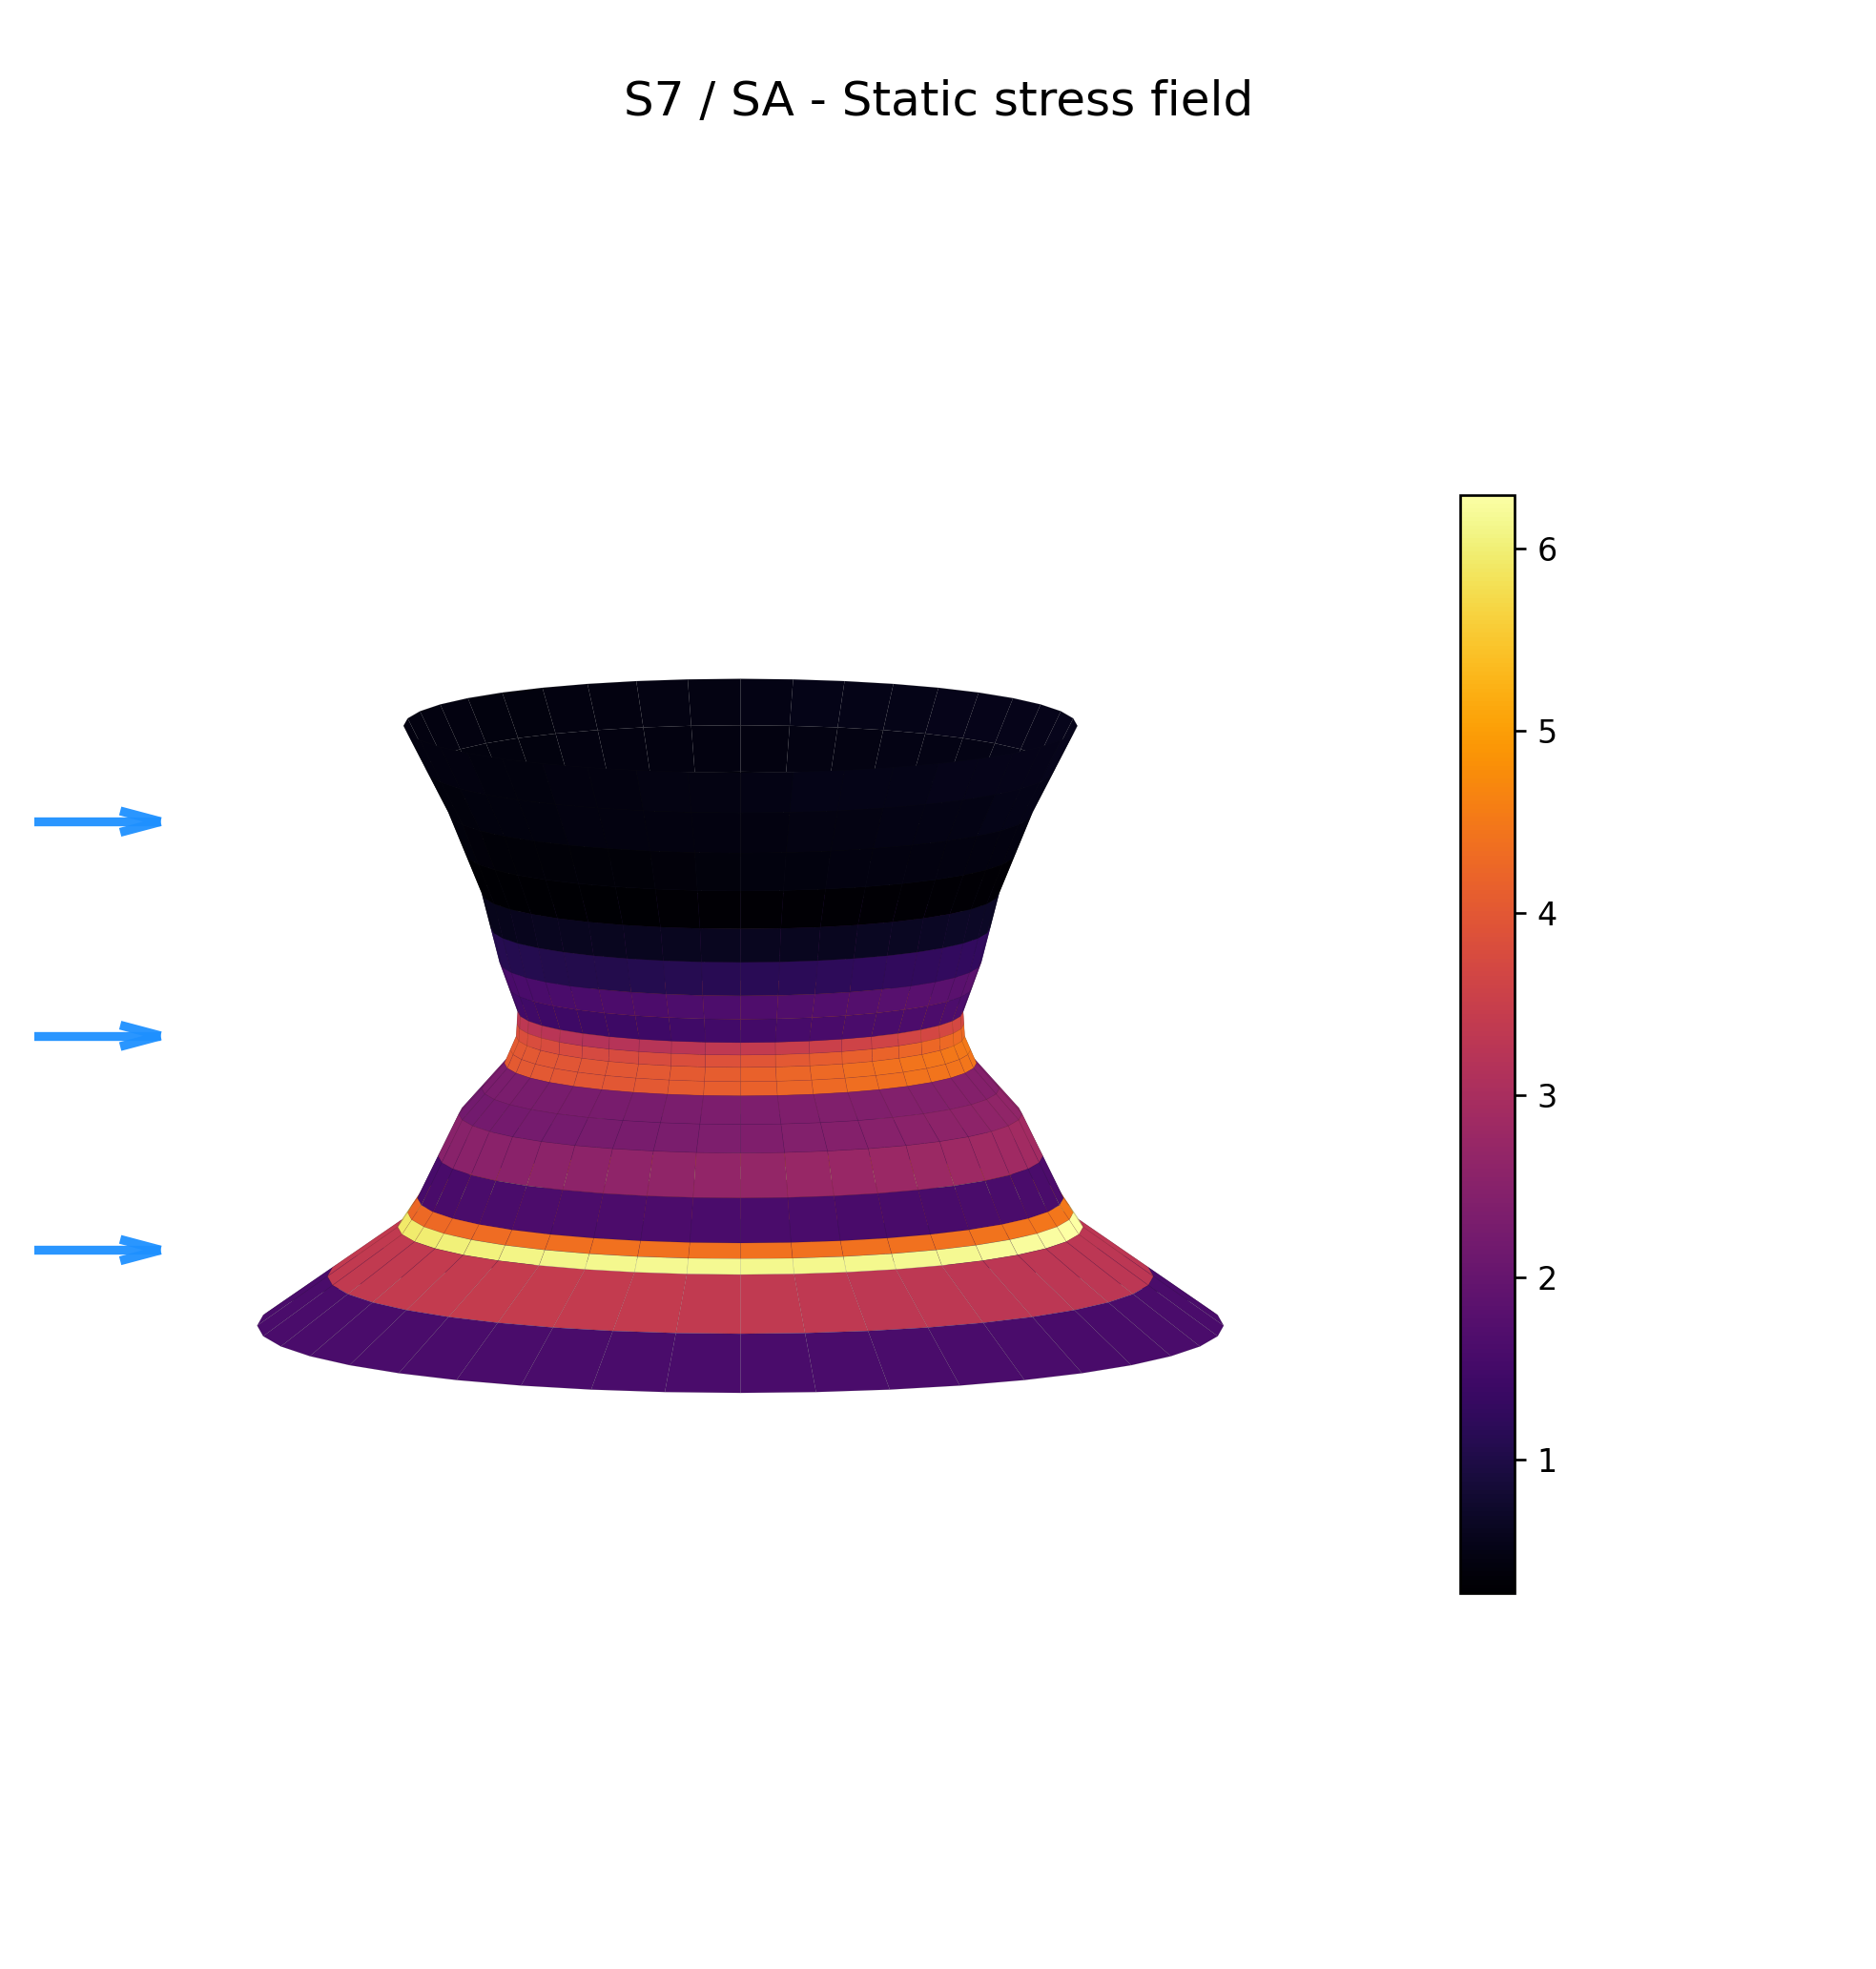
\includegraphics[width=\textwidth]{../results/figures/task7_s7_sa_stress.png}
\caption{S7 / SA stress}
\end{subfigure}\hfill
\begin{subfigure}{0.32\textwidth}
\centering
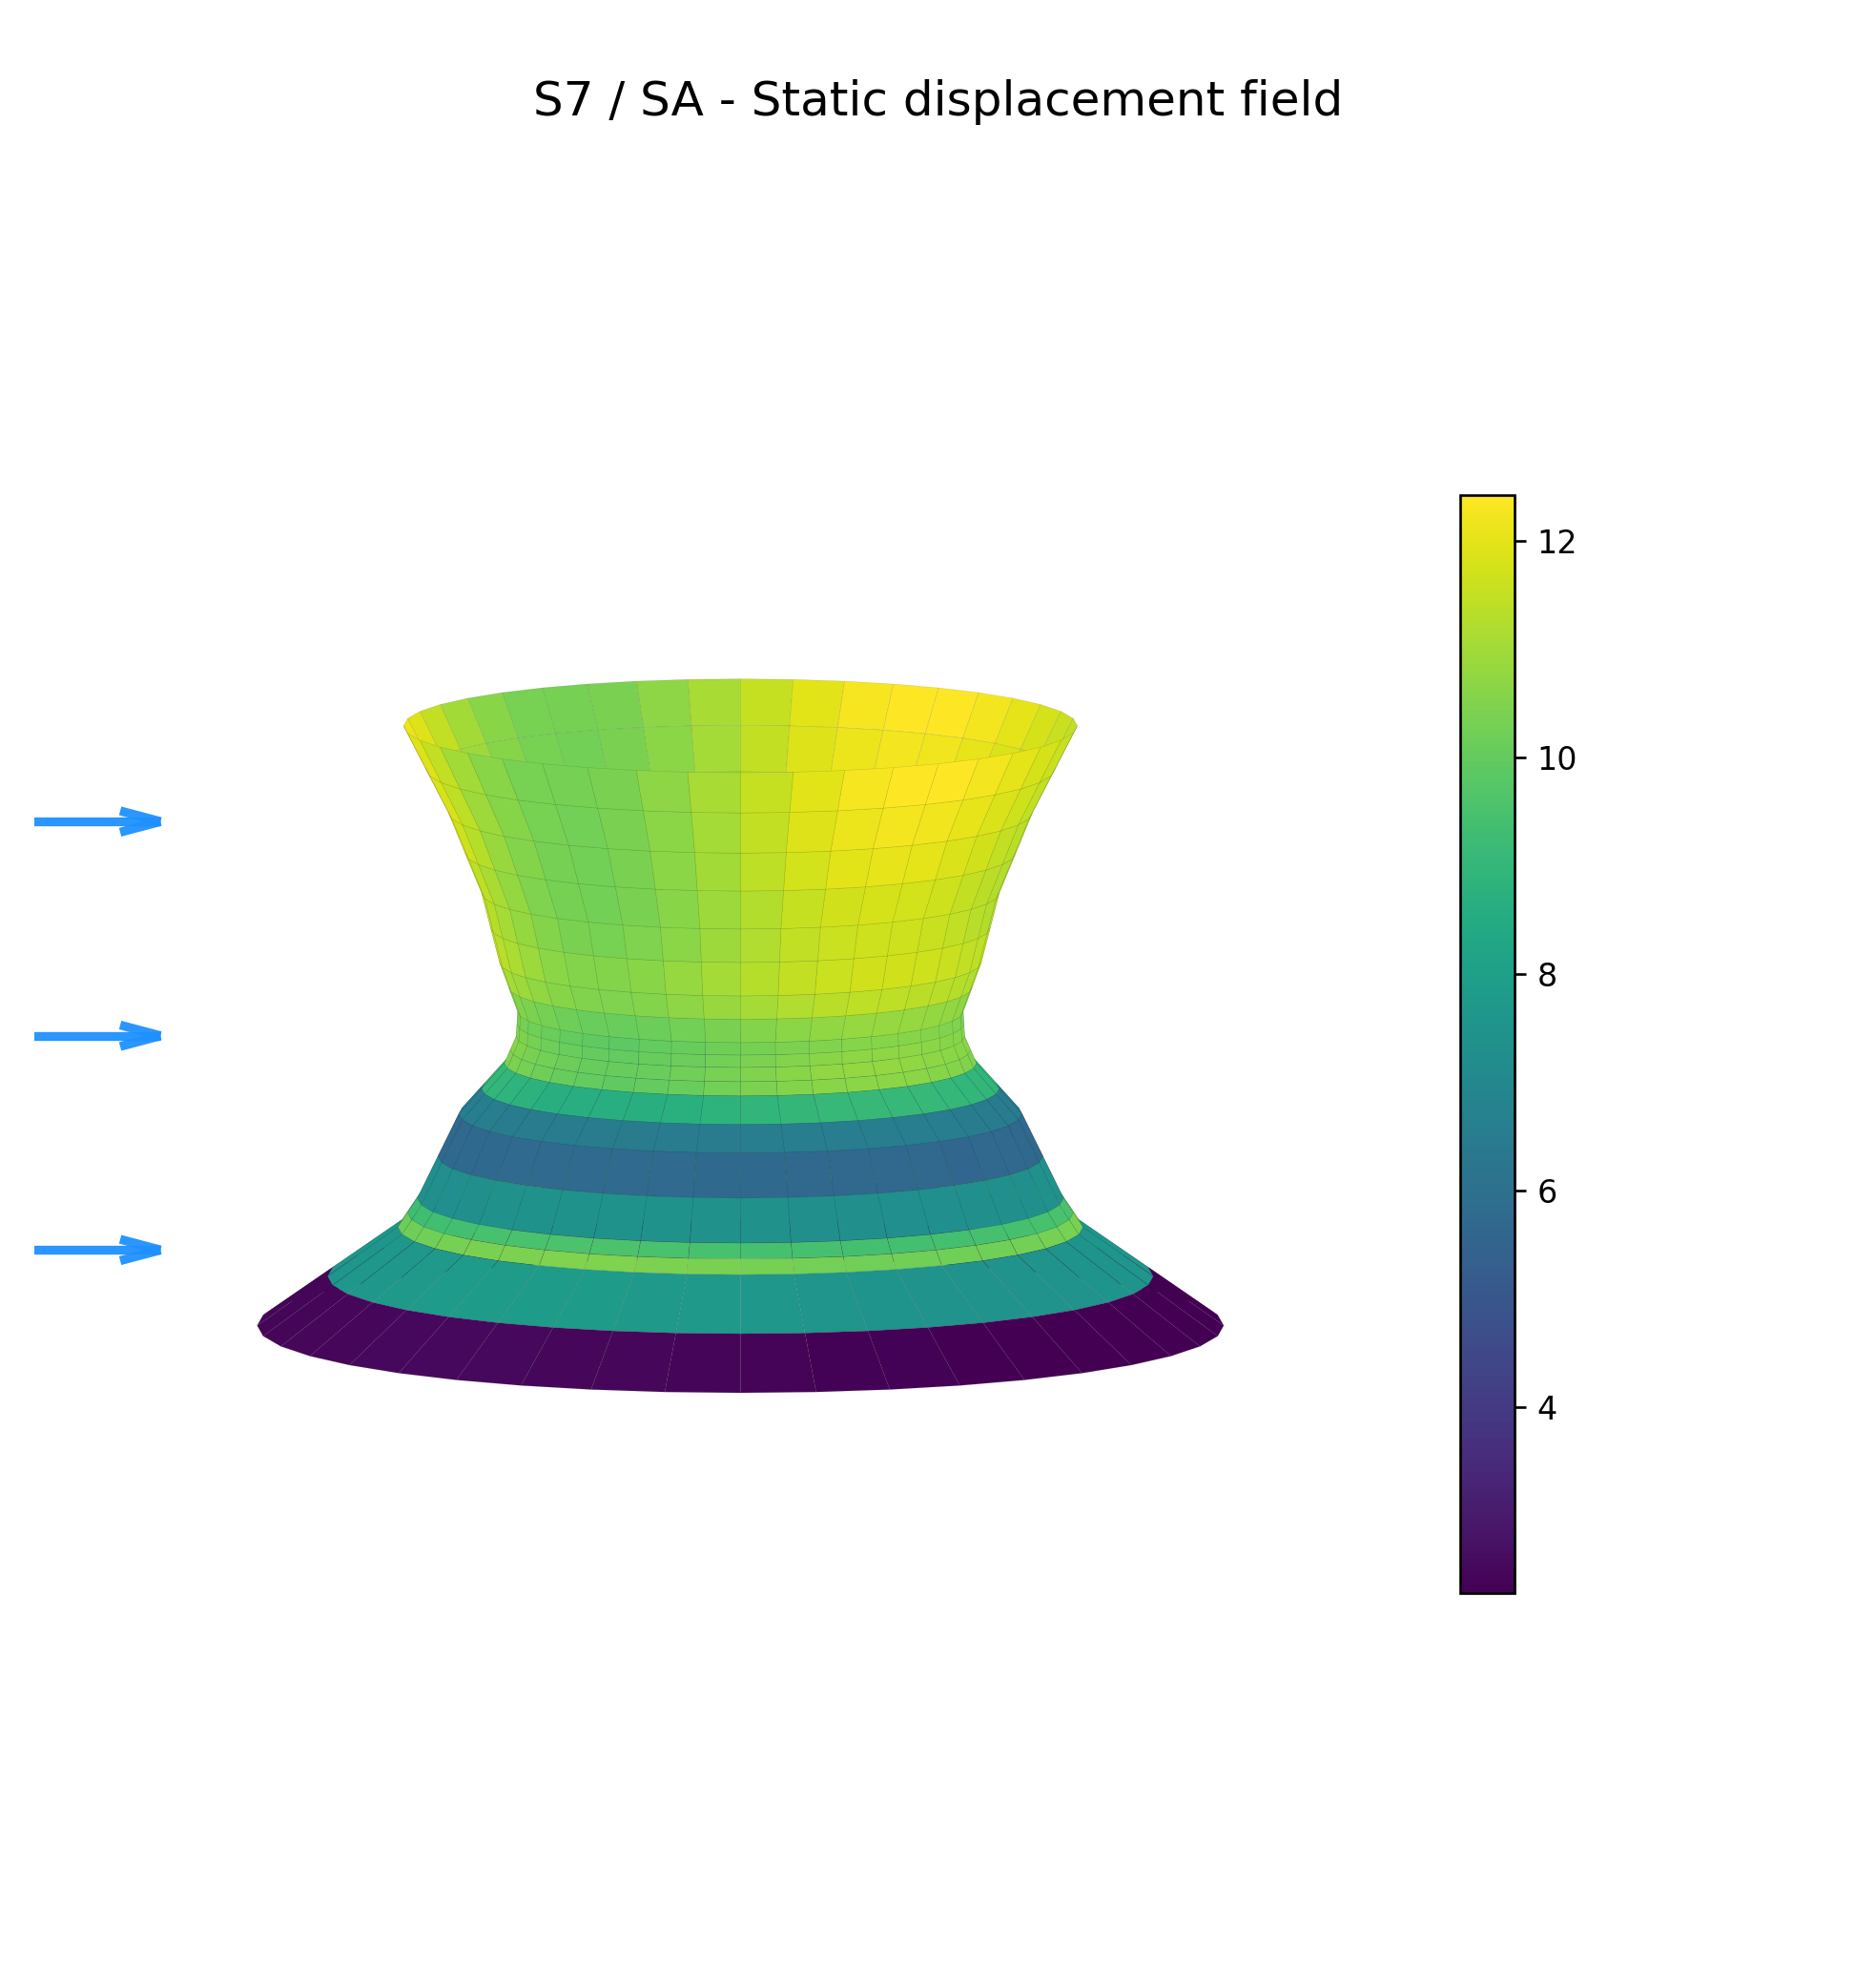
\includegraphics[width=\textwidth]{../results/figures/task7_s7_sa_displacement.png}
\caption{S7 / SA displacement}
\end{subfigure}\hfill
\begin{subfigure}{0.32\textwidth}
\centering
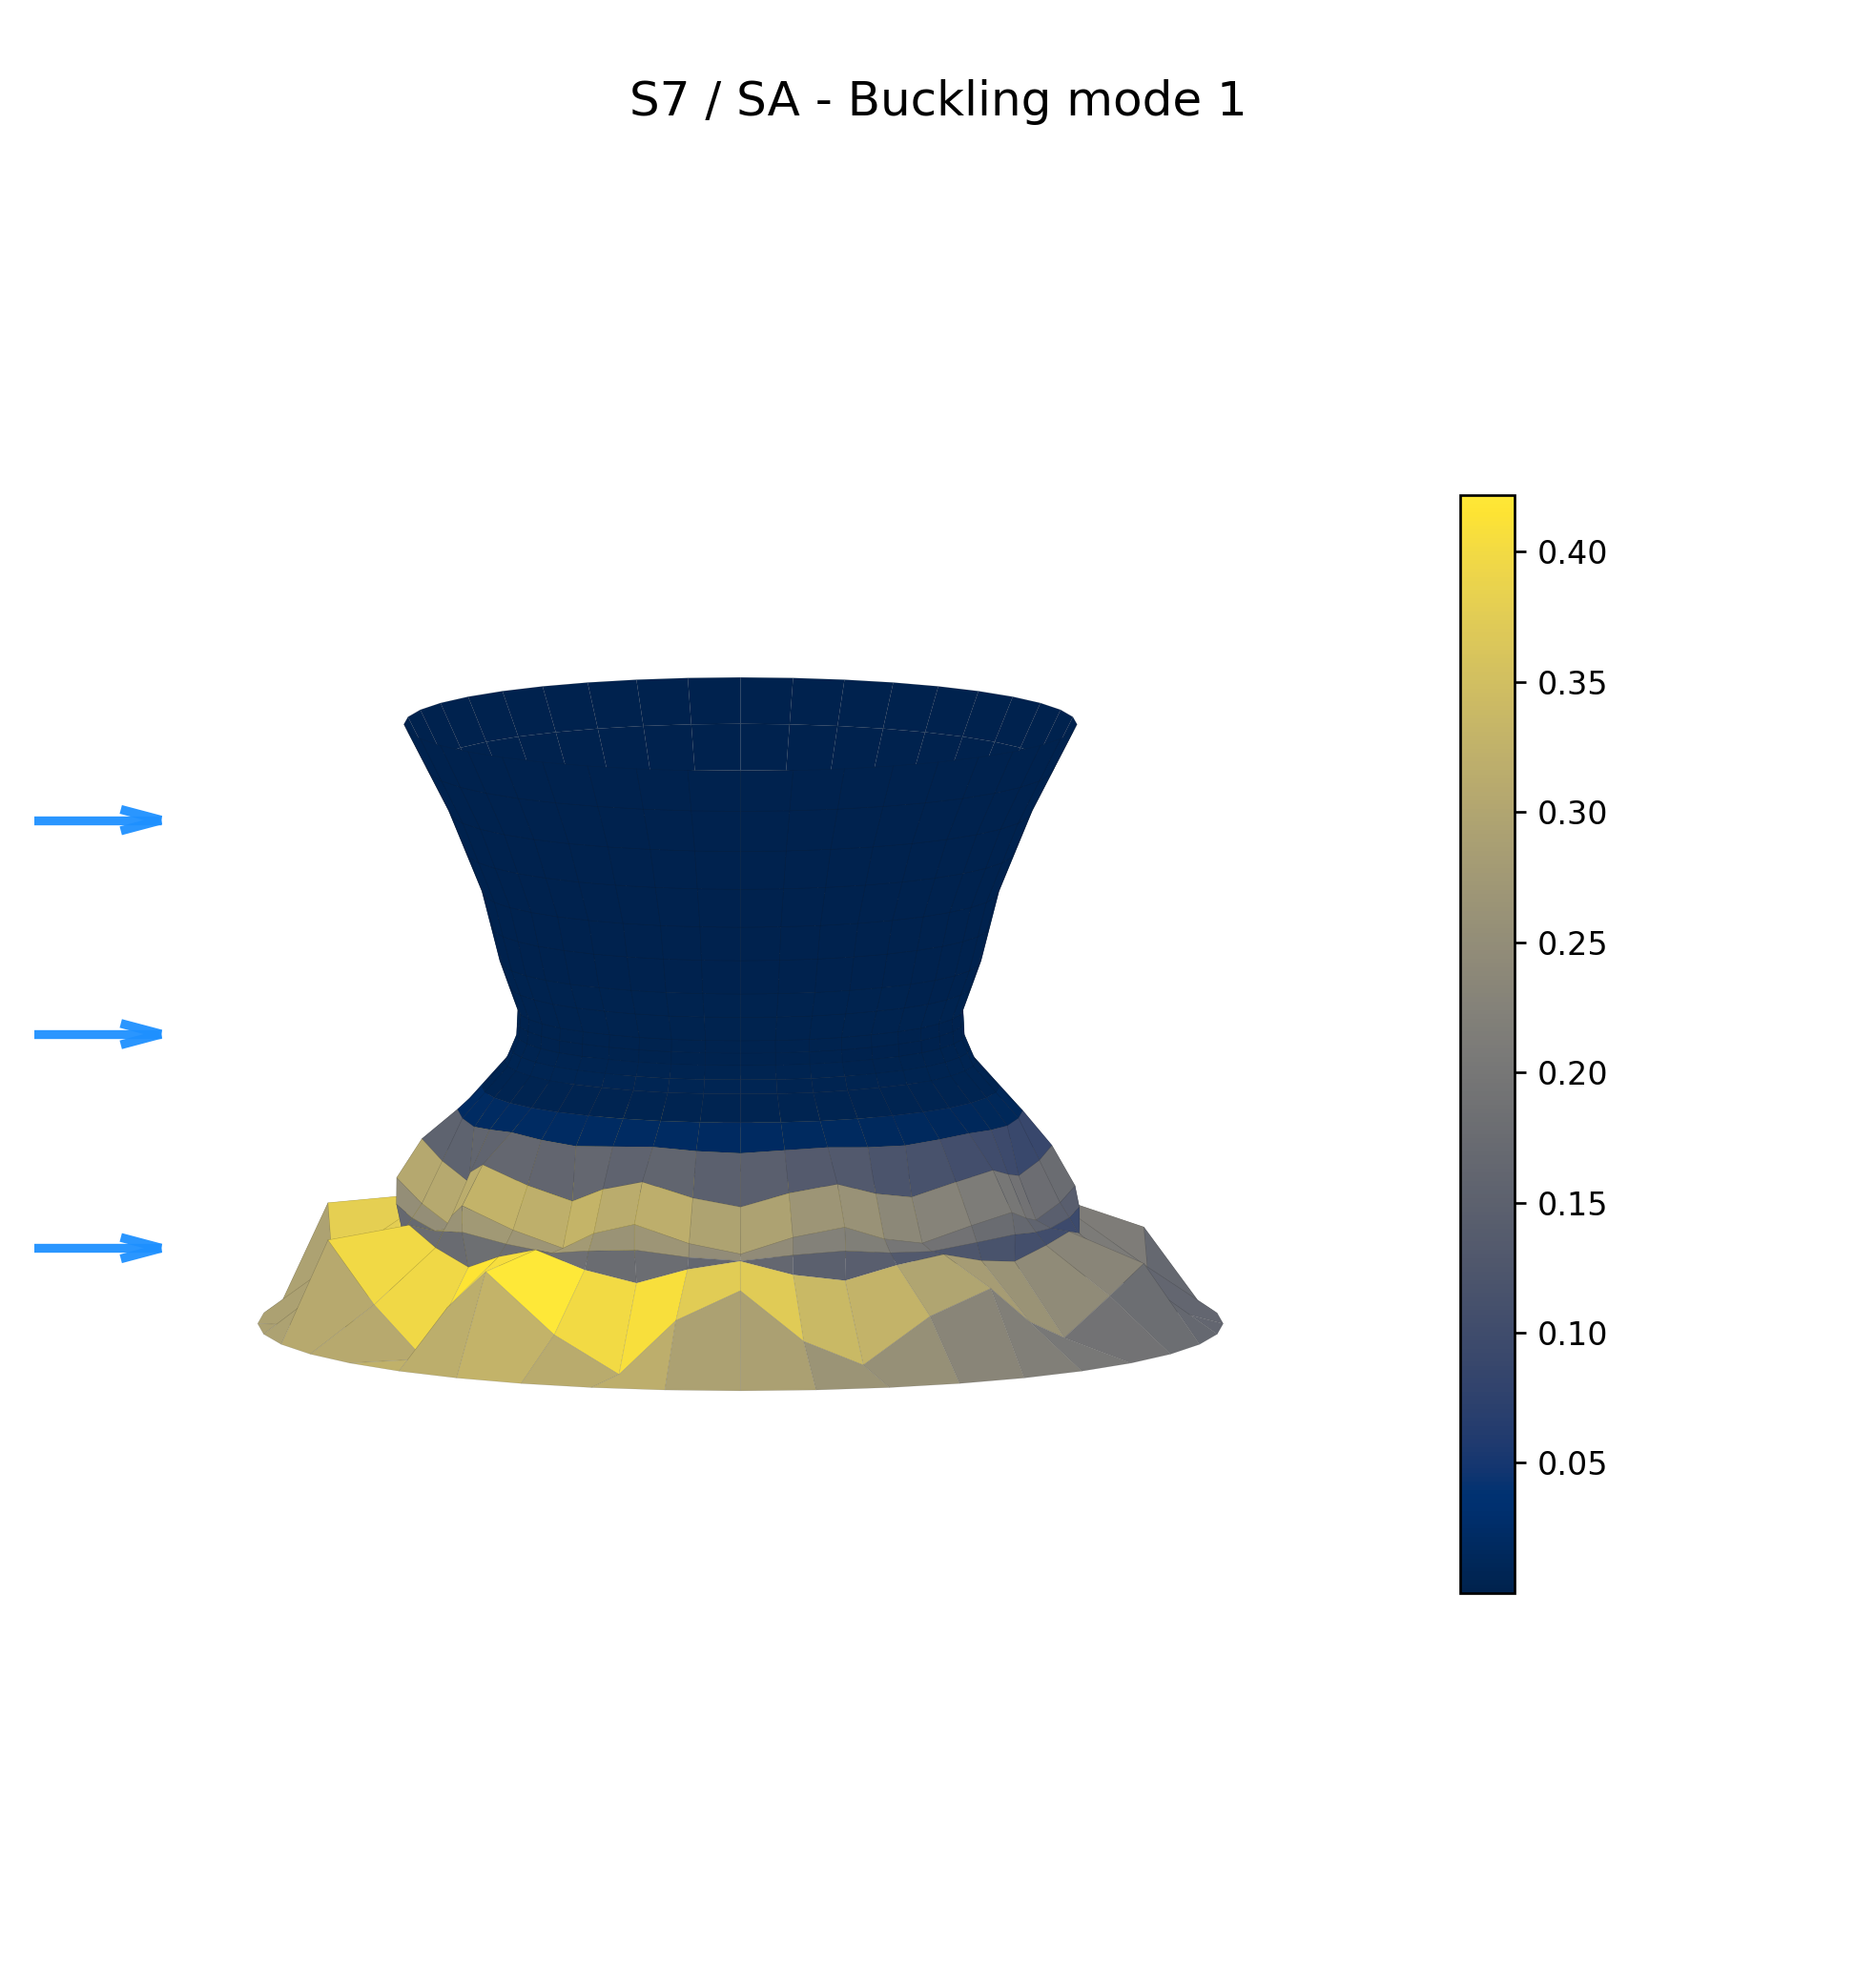
\includegraphics[width=\textwidth]{../results/figures/task7_s7_sa_buckling_mode1.png}
\caption{S7 / SA buckling}
\end{subfigure}
\caption{Combined visual fields}
\end{figure}


\section{Scenario S8}


\subsection{S8 / BFGS}


\begin{figure}[H]
\centering
\begin{subfigure}{0.32\textwidth}
\centering
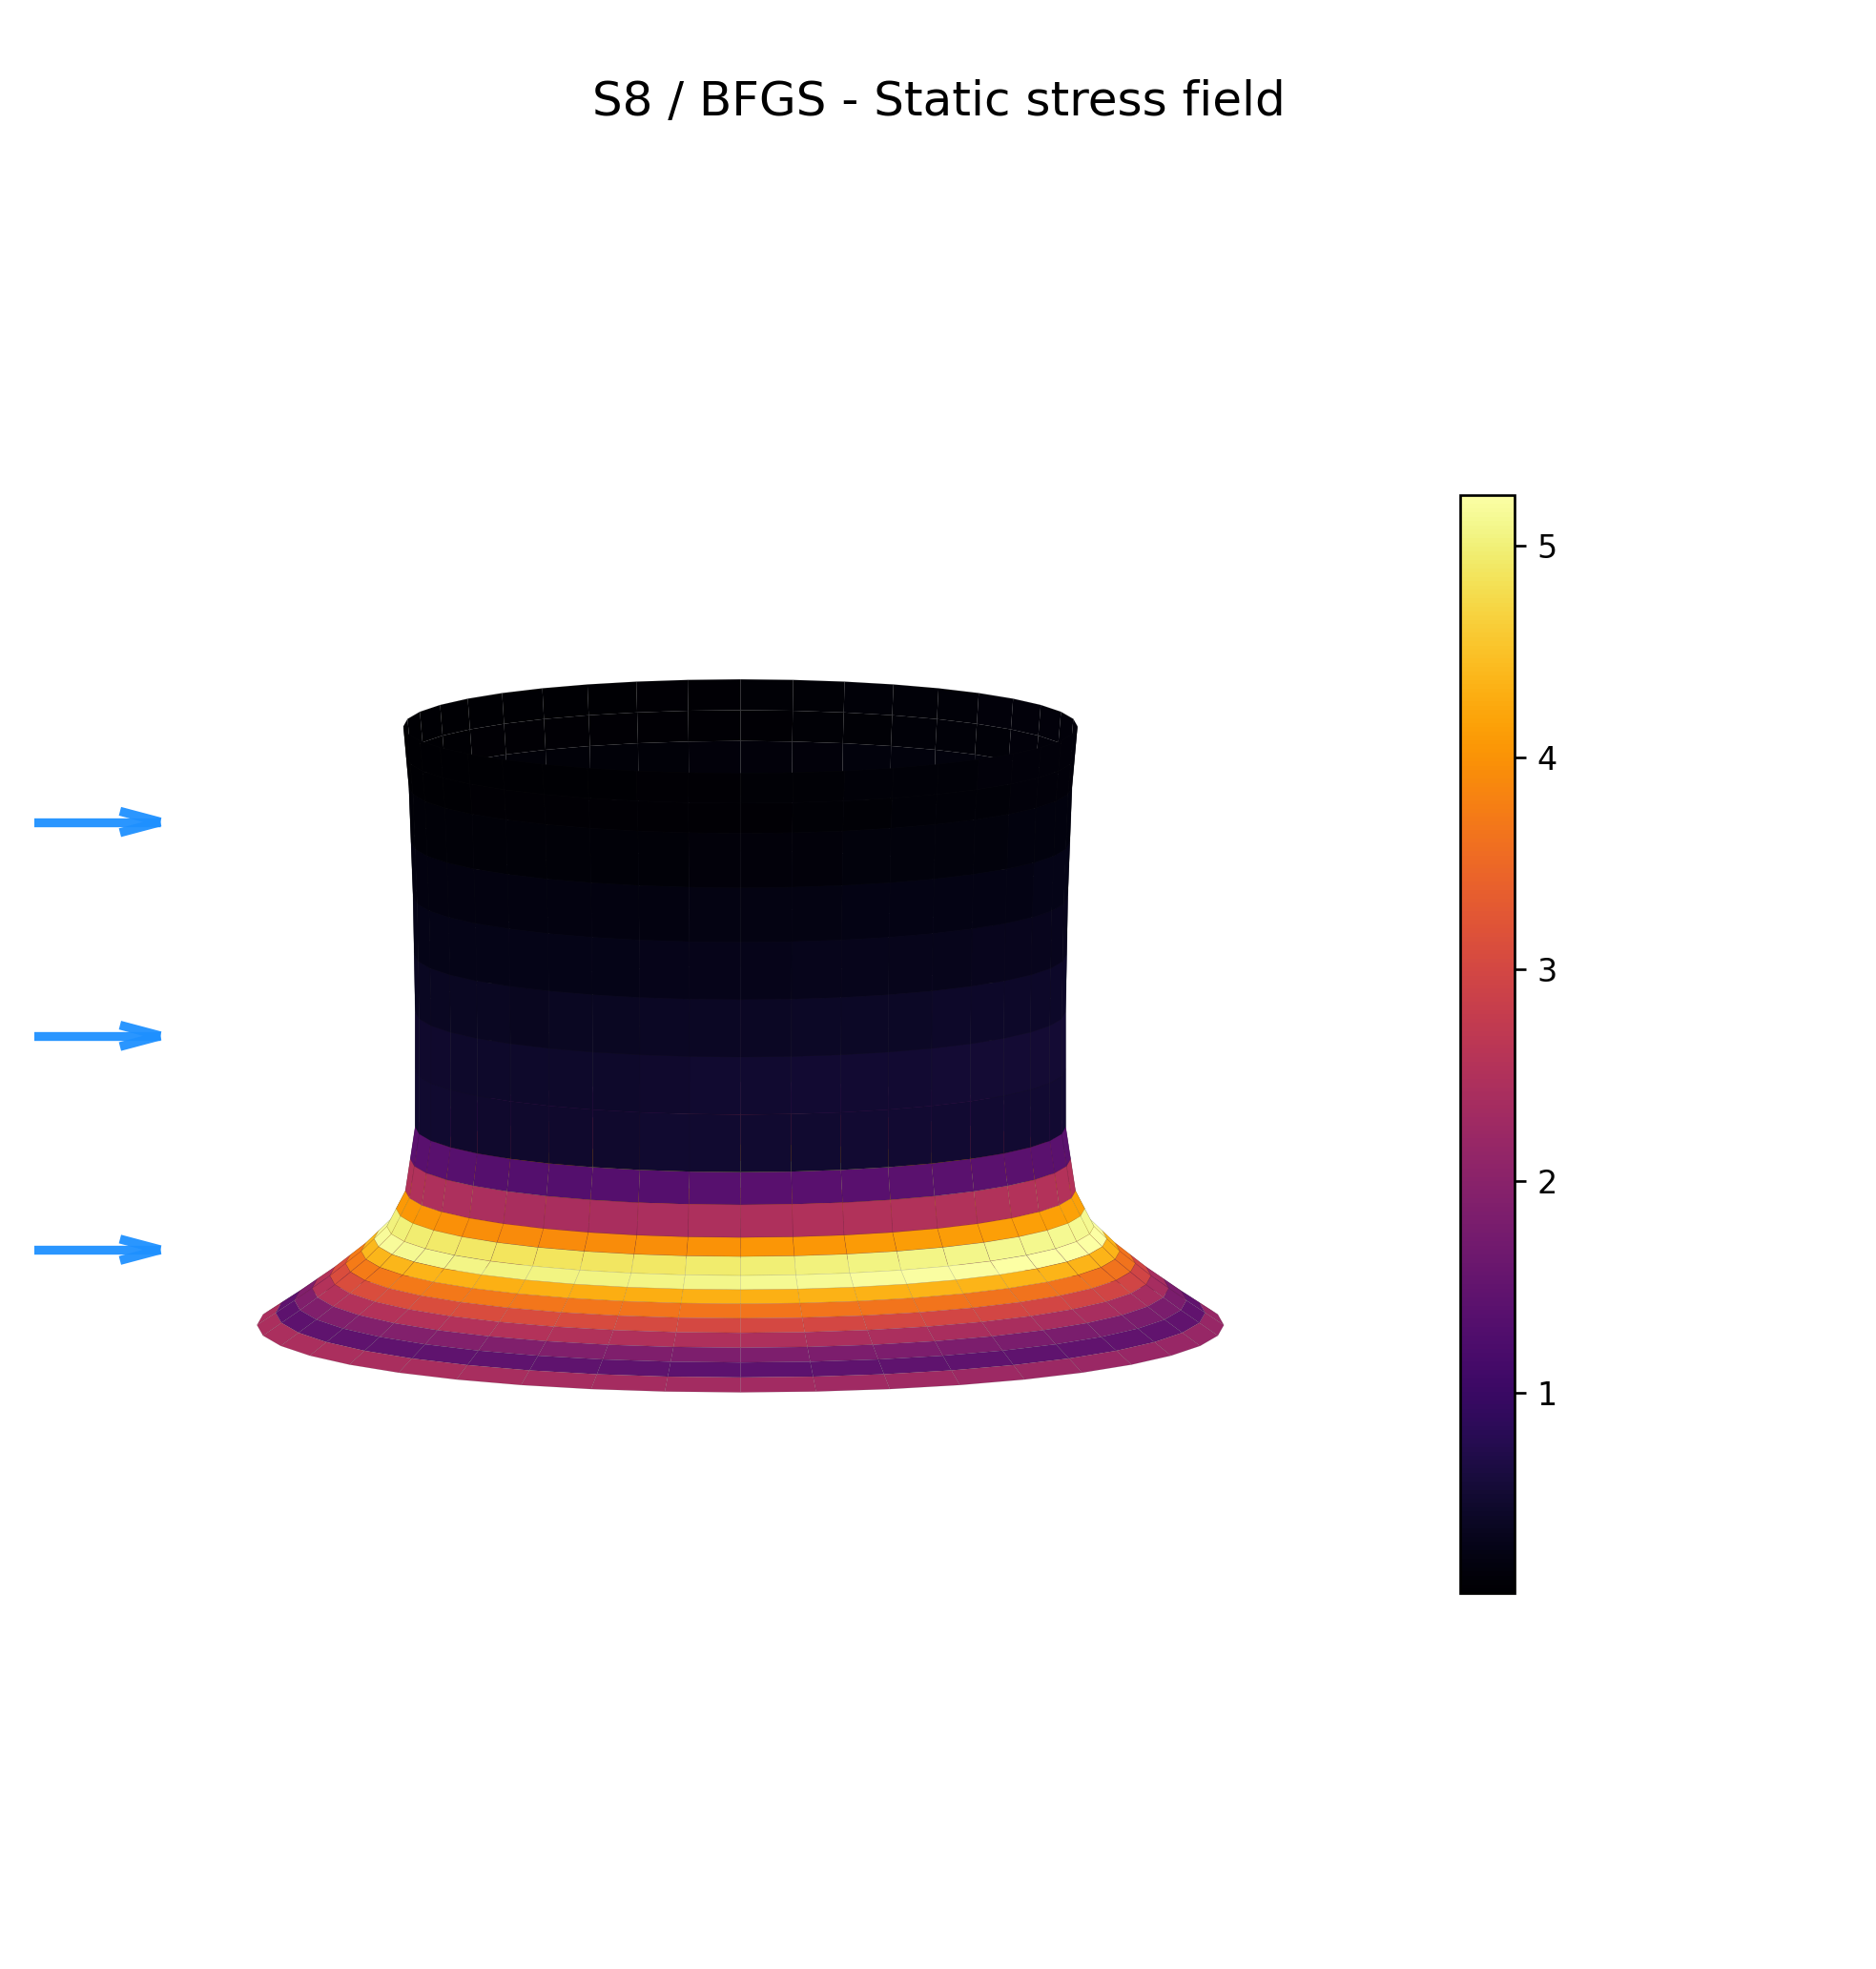
\includegraphics[width=\textwidth]{../results/figures/task7_s8_bfgs_stress.png}
\caption{S8 / BFGS stress}
\end{subfigure}\hfill
\begin{subfigure}{0.32\textwidth}
\centering
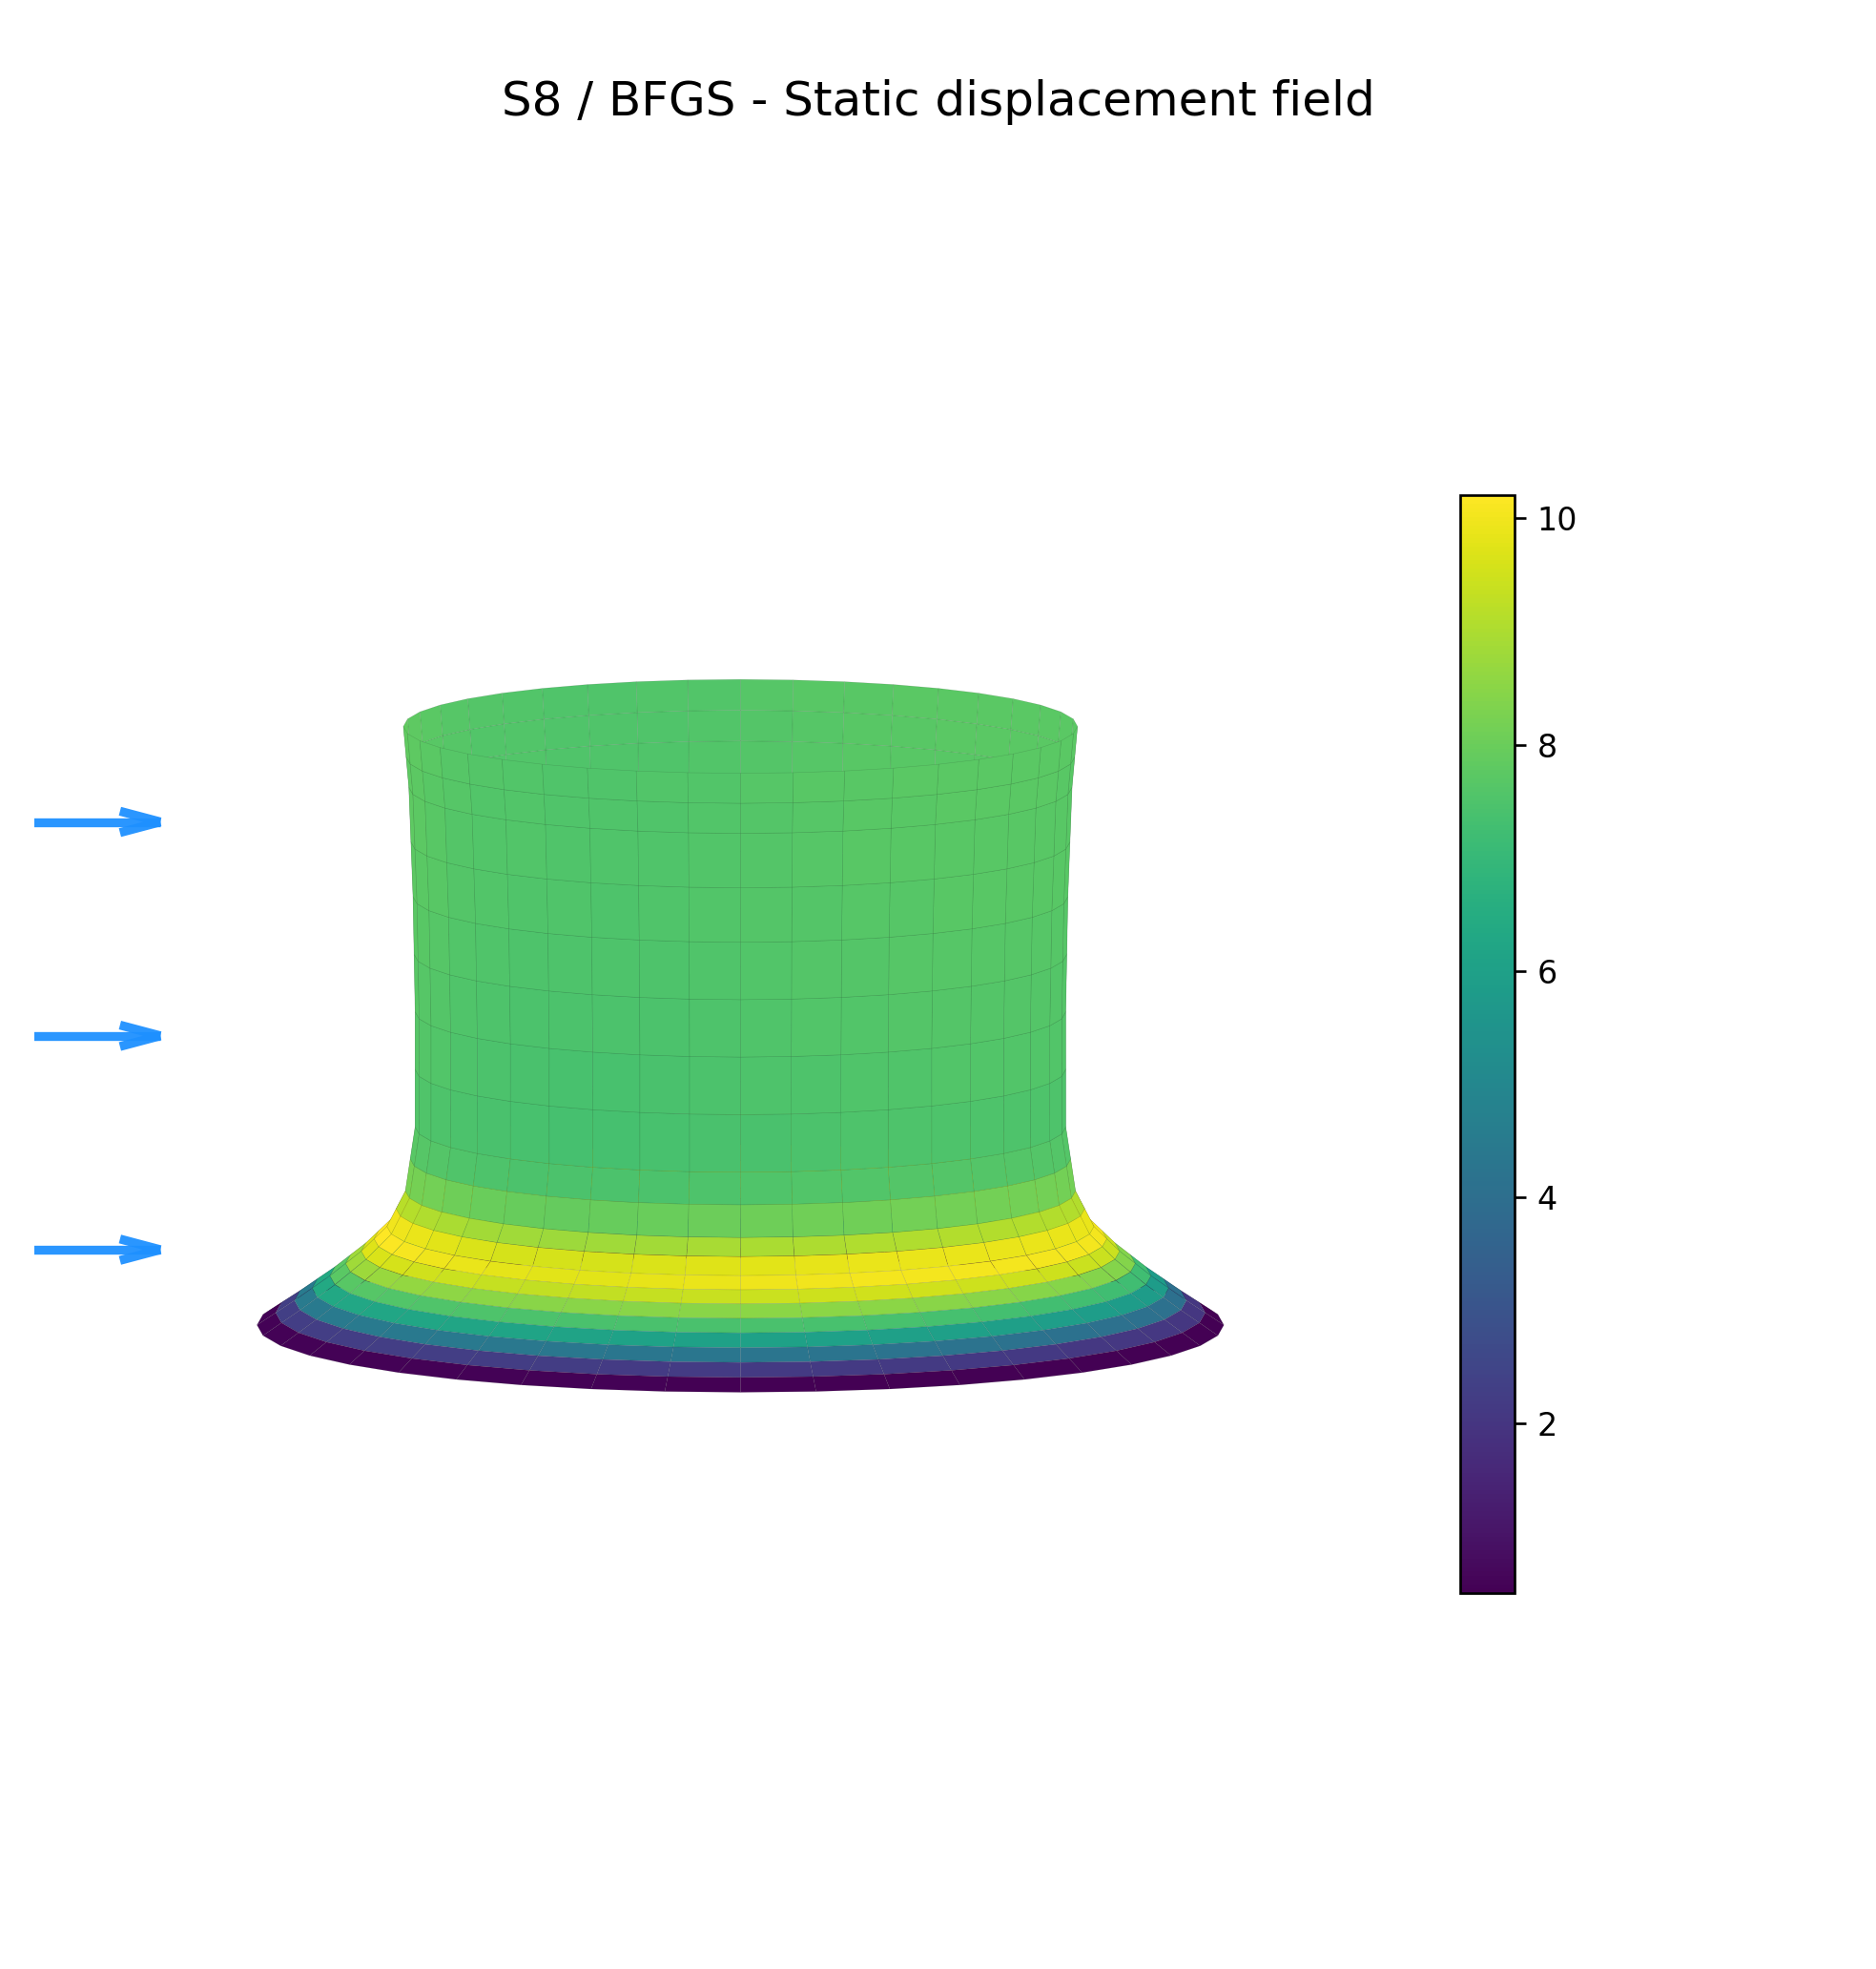
\includegraphics[width=\textwidth]{../results/figures/task7_s8_bfgs_displacement.png}
\caption{S8 / BFGS displacement}
\end{subfigure}\hfill
\begin{subfigure}{0.32\textwidth}
\centering
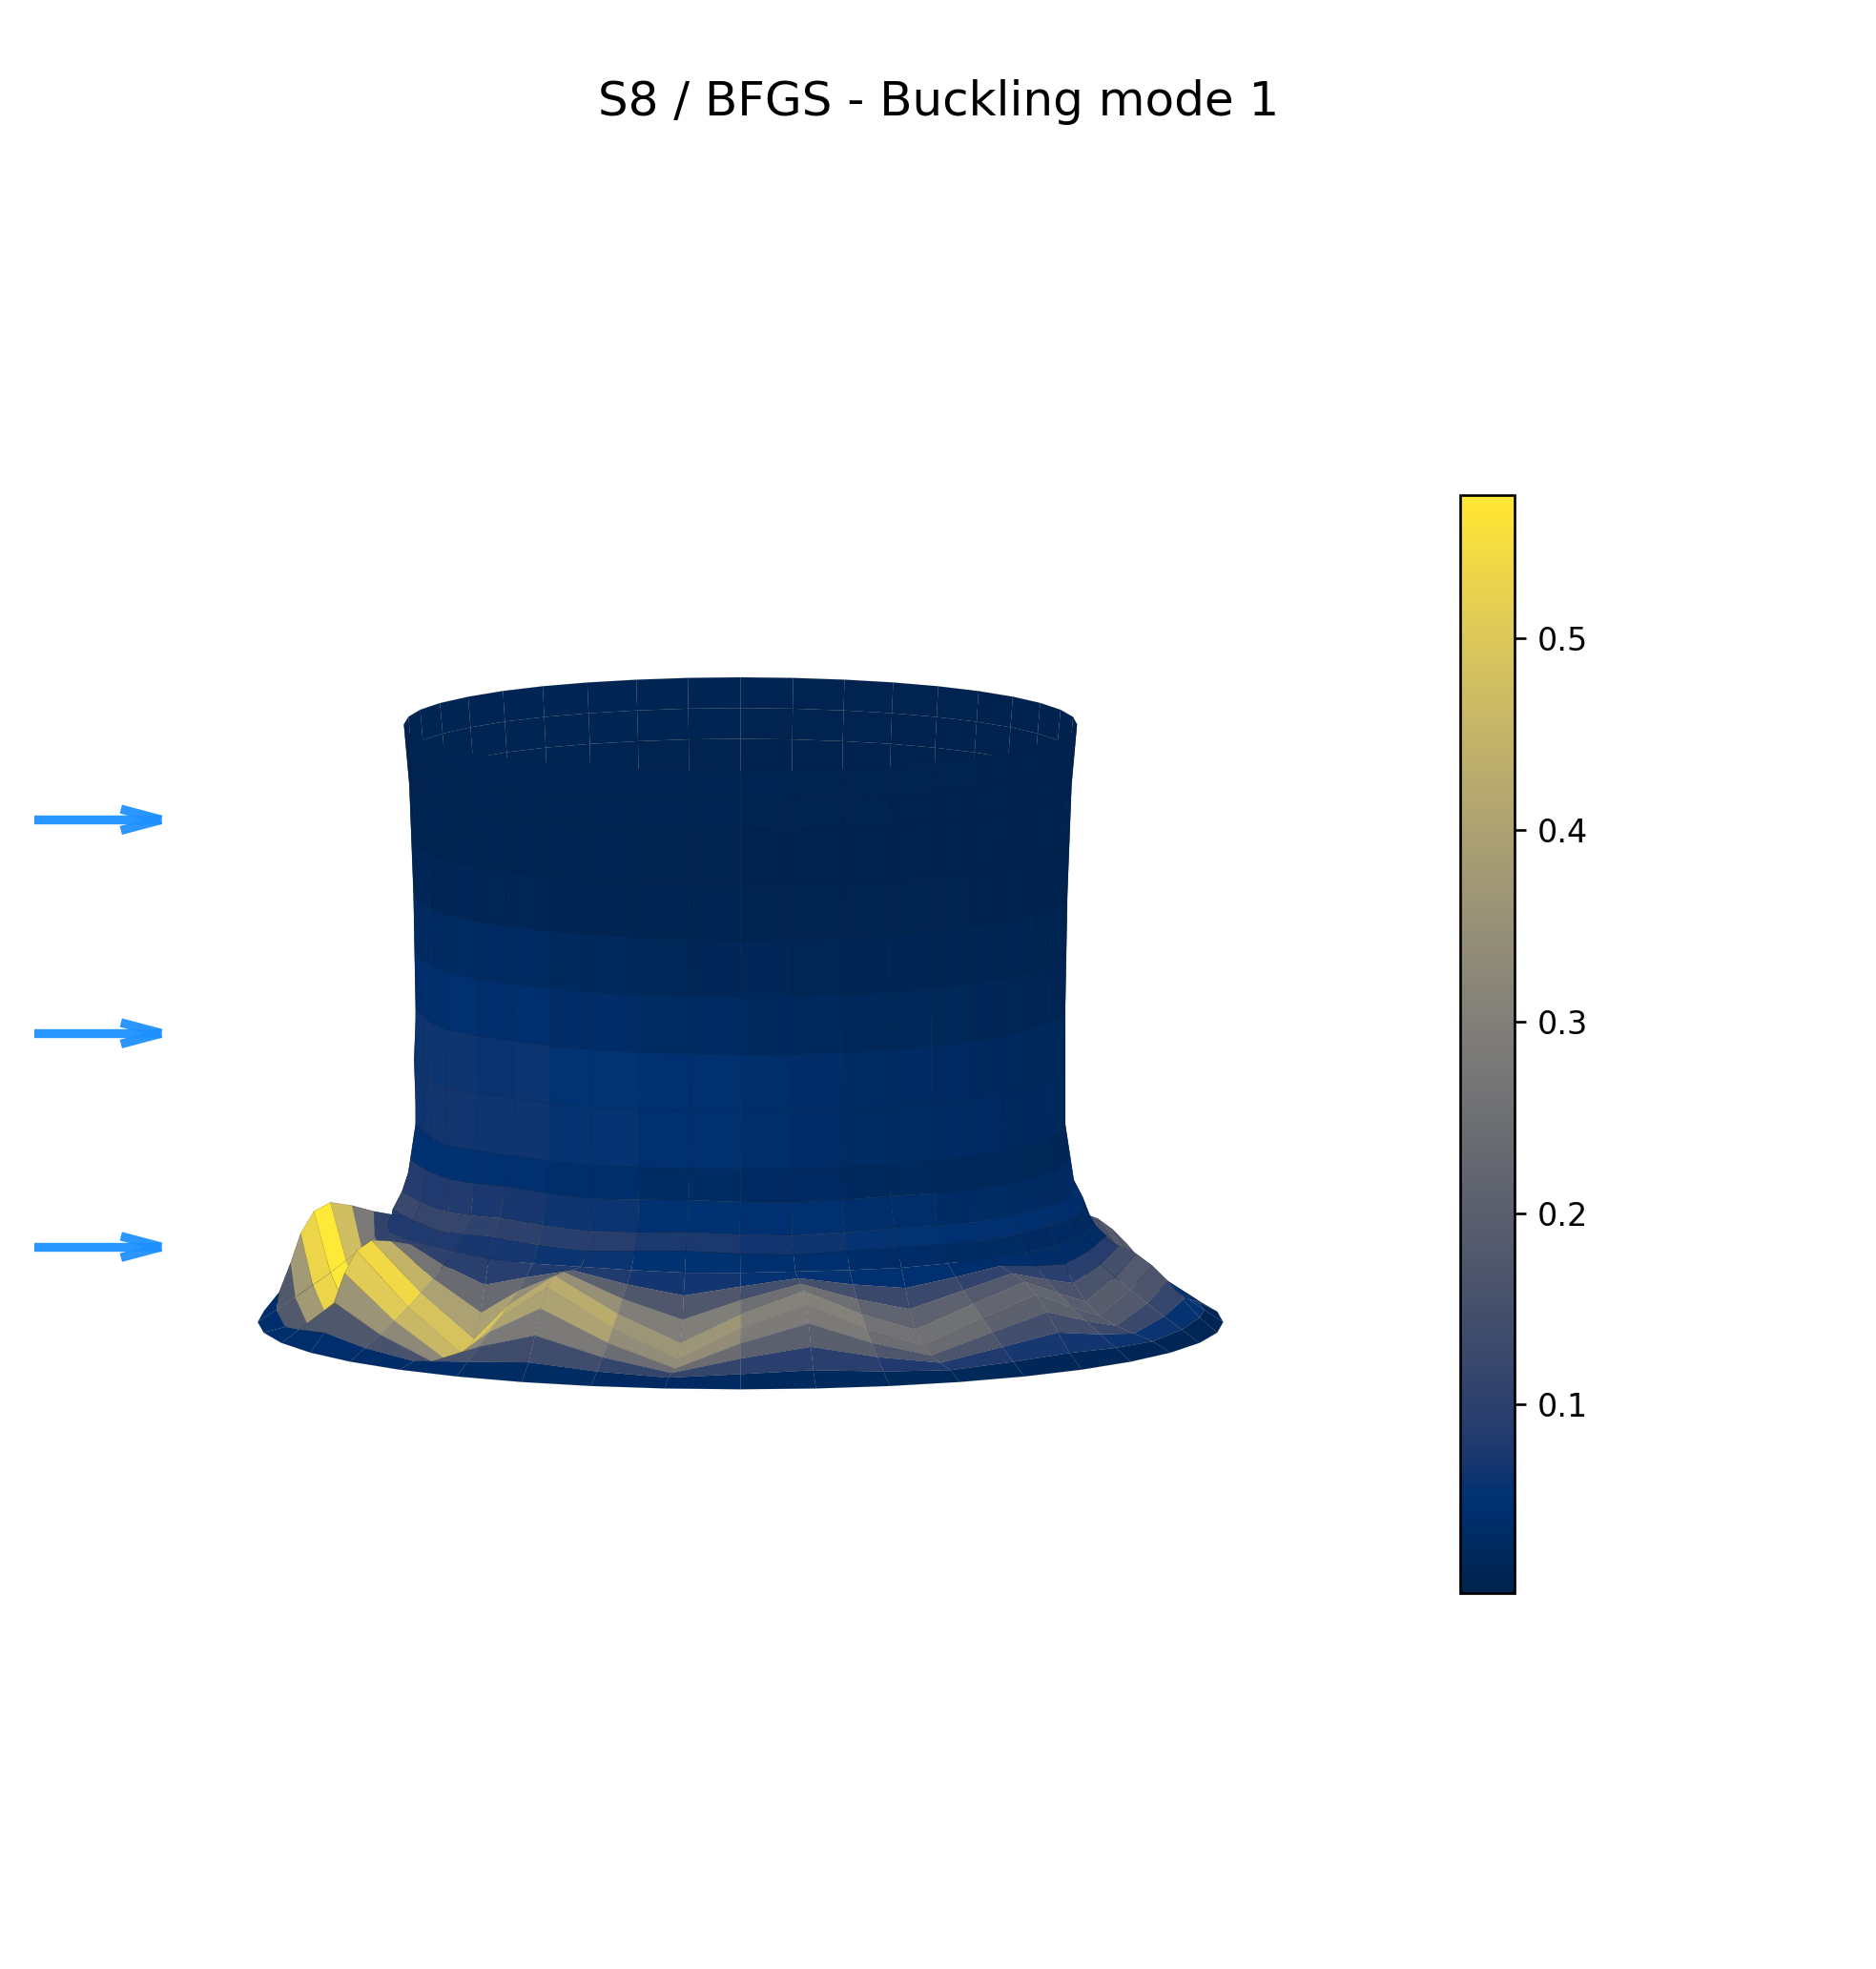
\includegraphics[width=\textwidth]{../results/figures/task7_s8_bfgs_buckling_mode1.png}
\caption{S8 / BFGS buckling}
\end{subfigure}
\caption{Combined visual fields}
\end{figure}


\subsection{S8 / PSO}


\begin{figure}[H]
\centering
\begin{subfigure}{0.32\textwidth}
\centering
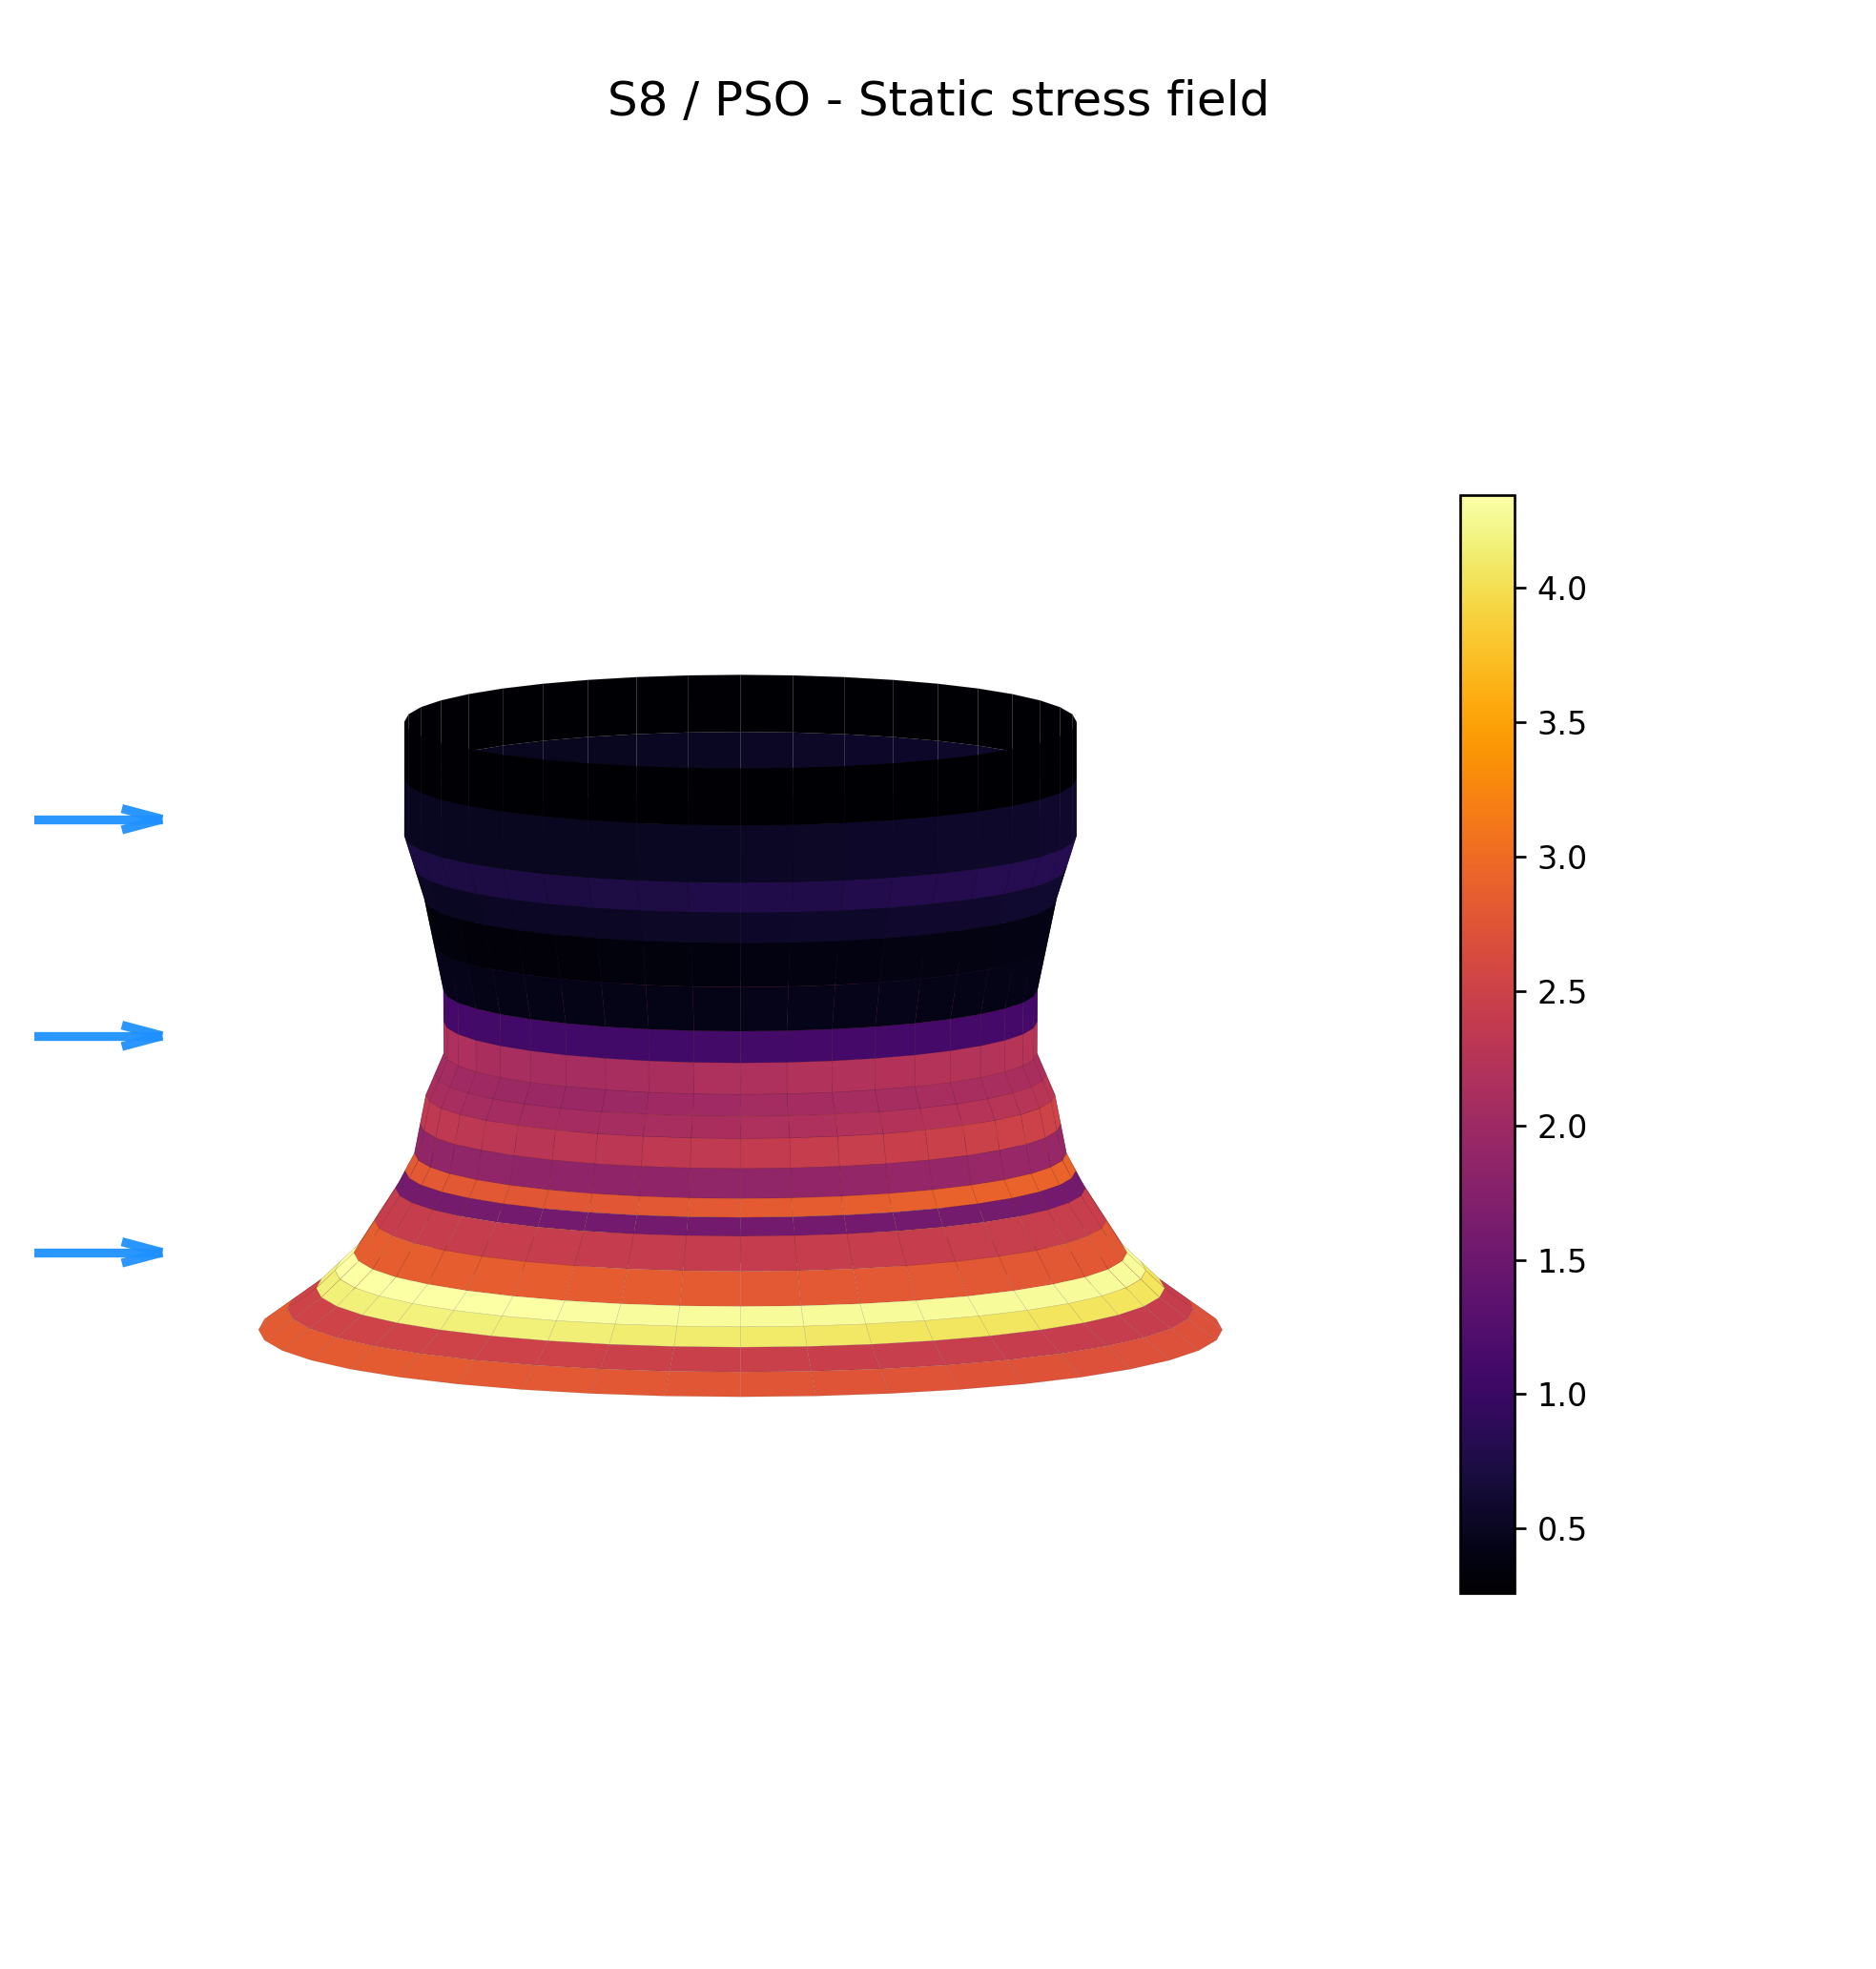
\includegraphics[width=\textwidth]{../results/figures/task7_s8_pso_stress.png}
\caption{S8 / PSO stress}
\end{subfigure}\hfill
\begin{subfigure}{0.32\textwidth}
\centering
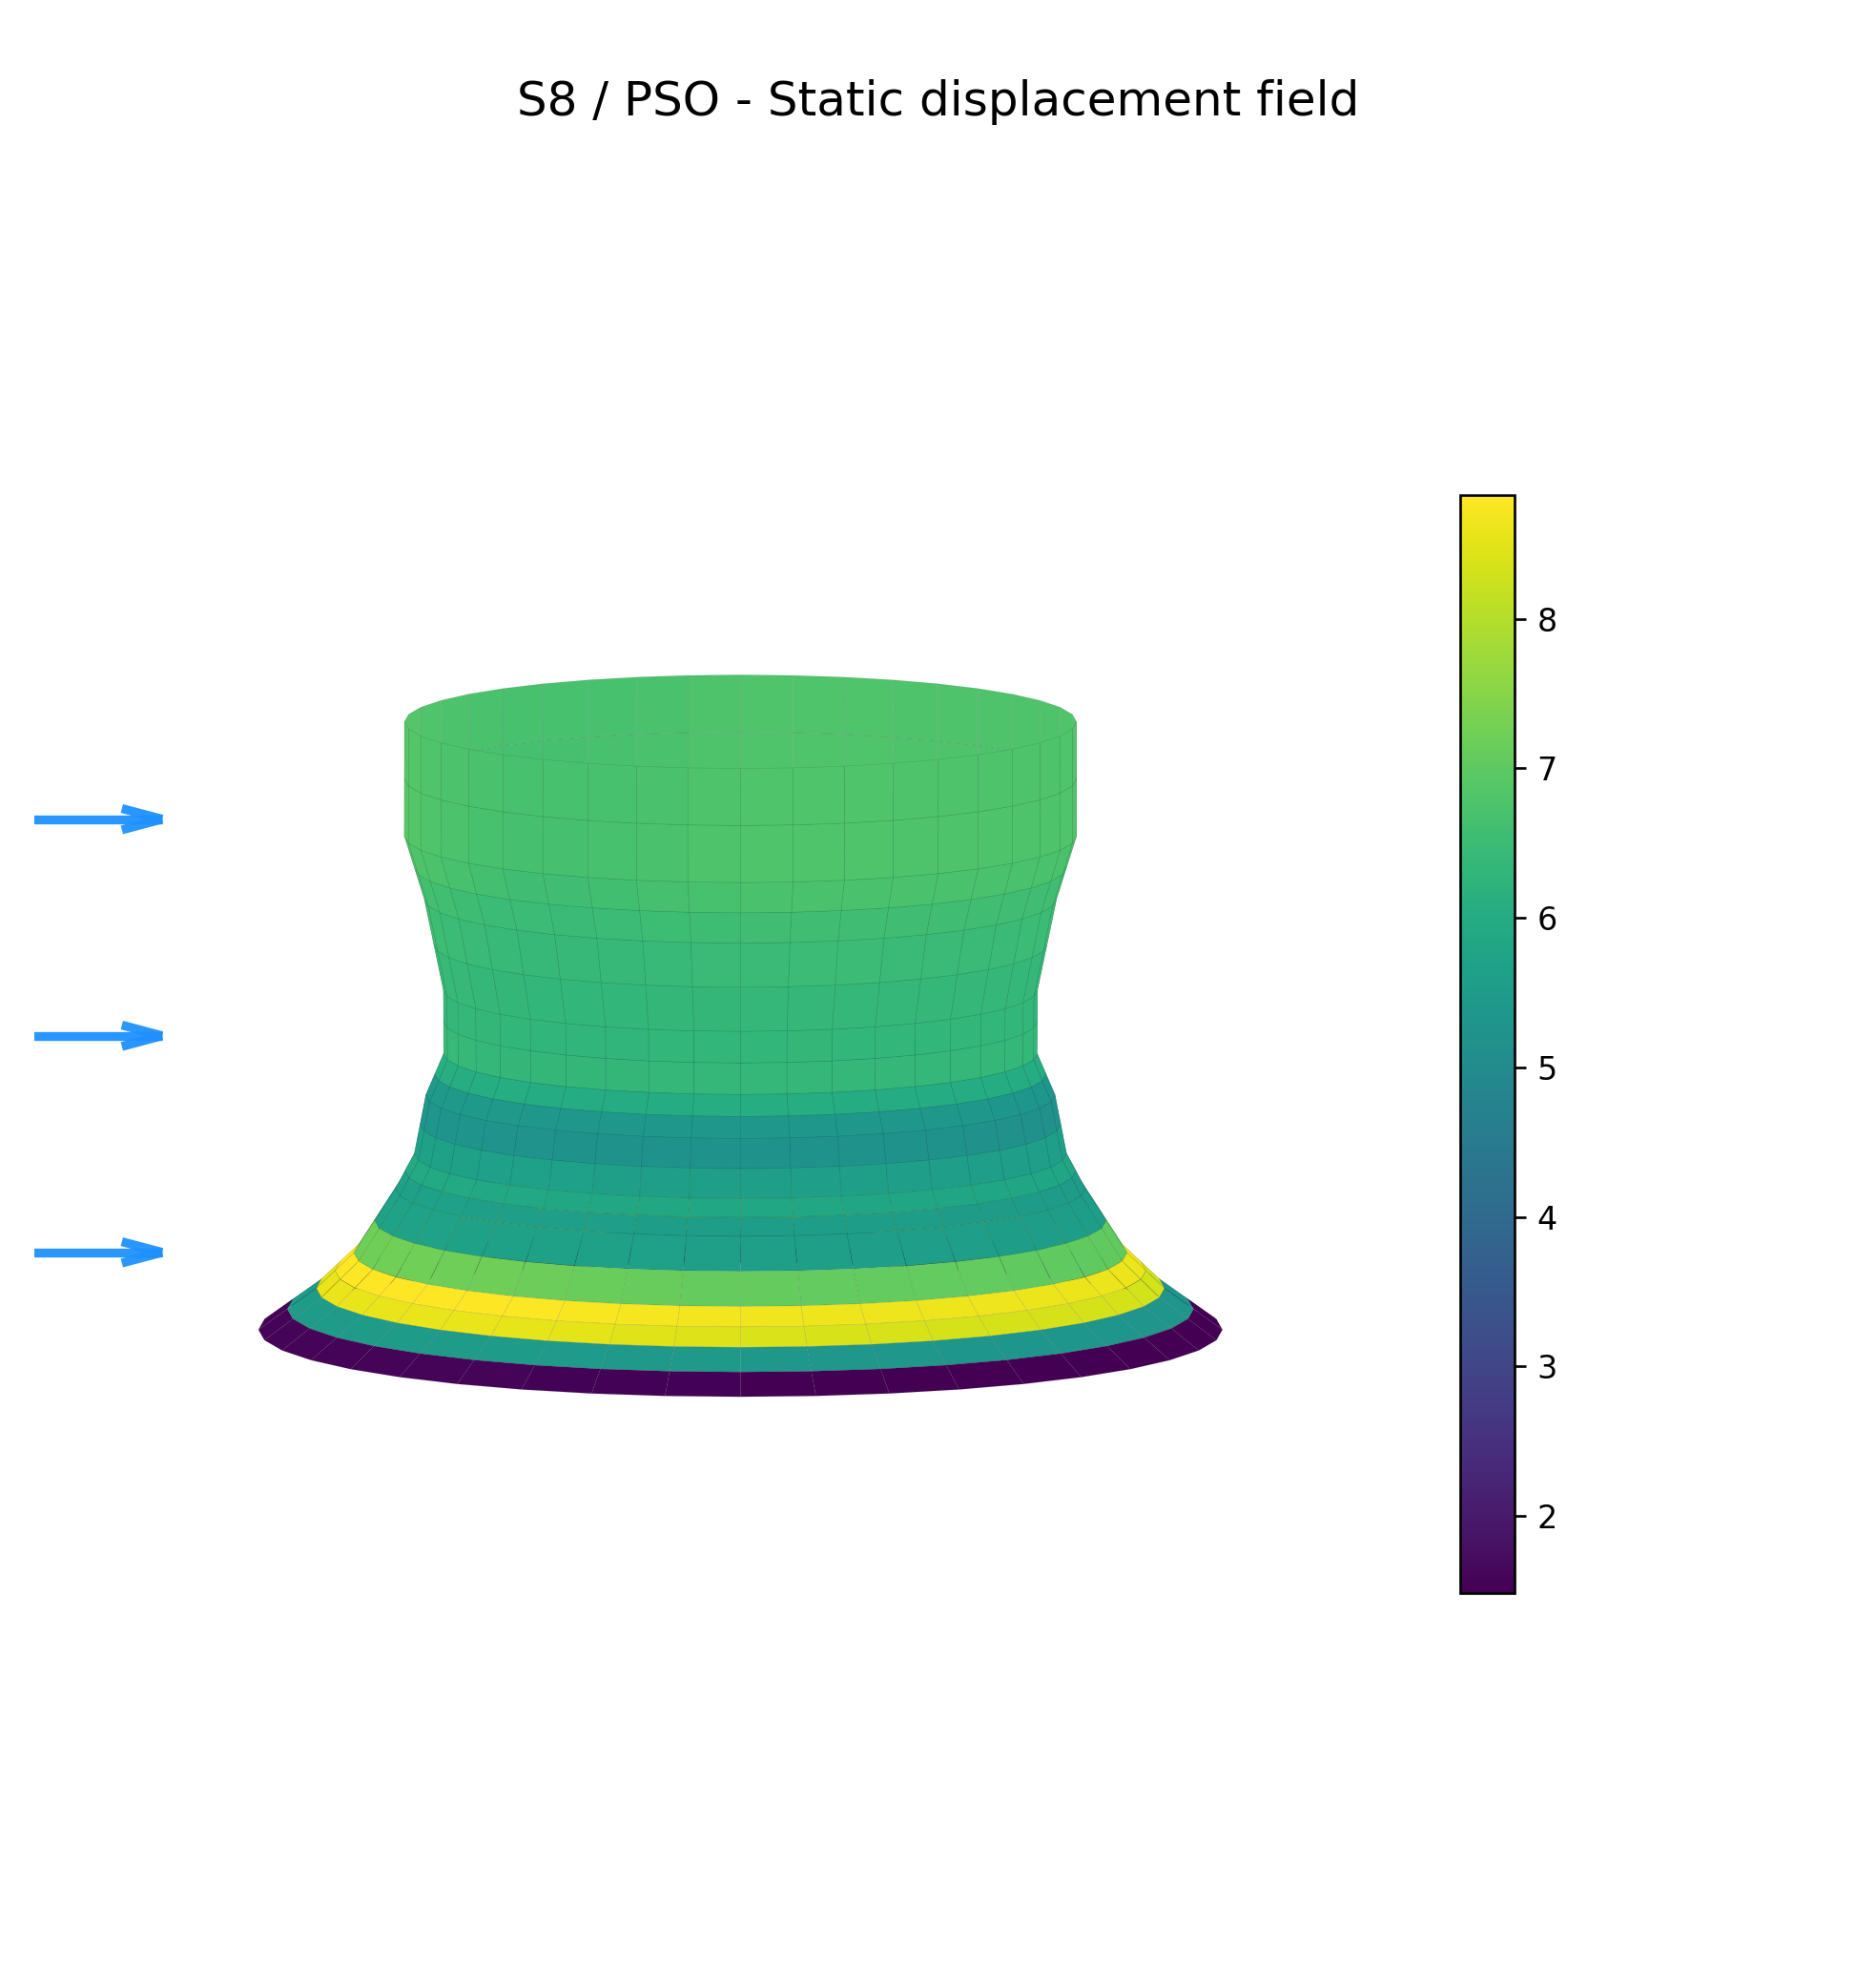
\includegraphics[width=\textwidth]{../results/figures/task7_s8_pso_displacement.png}
\caption{S8 / PSO displacement}
\end{subfigure}\hfill
\begin{subfigure}{0.32\textwidth}
\centering
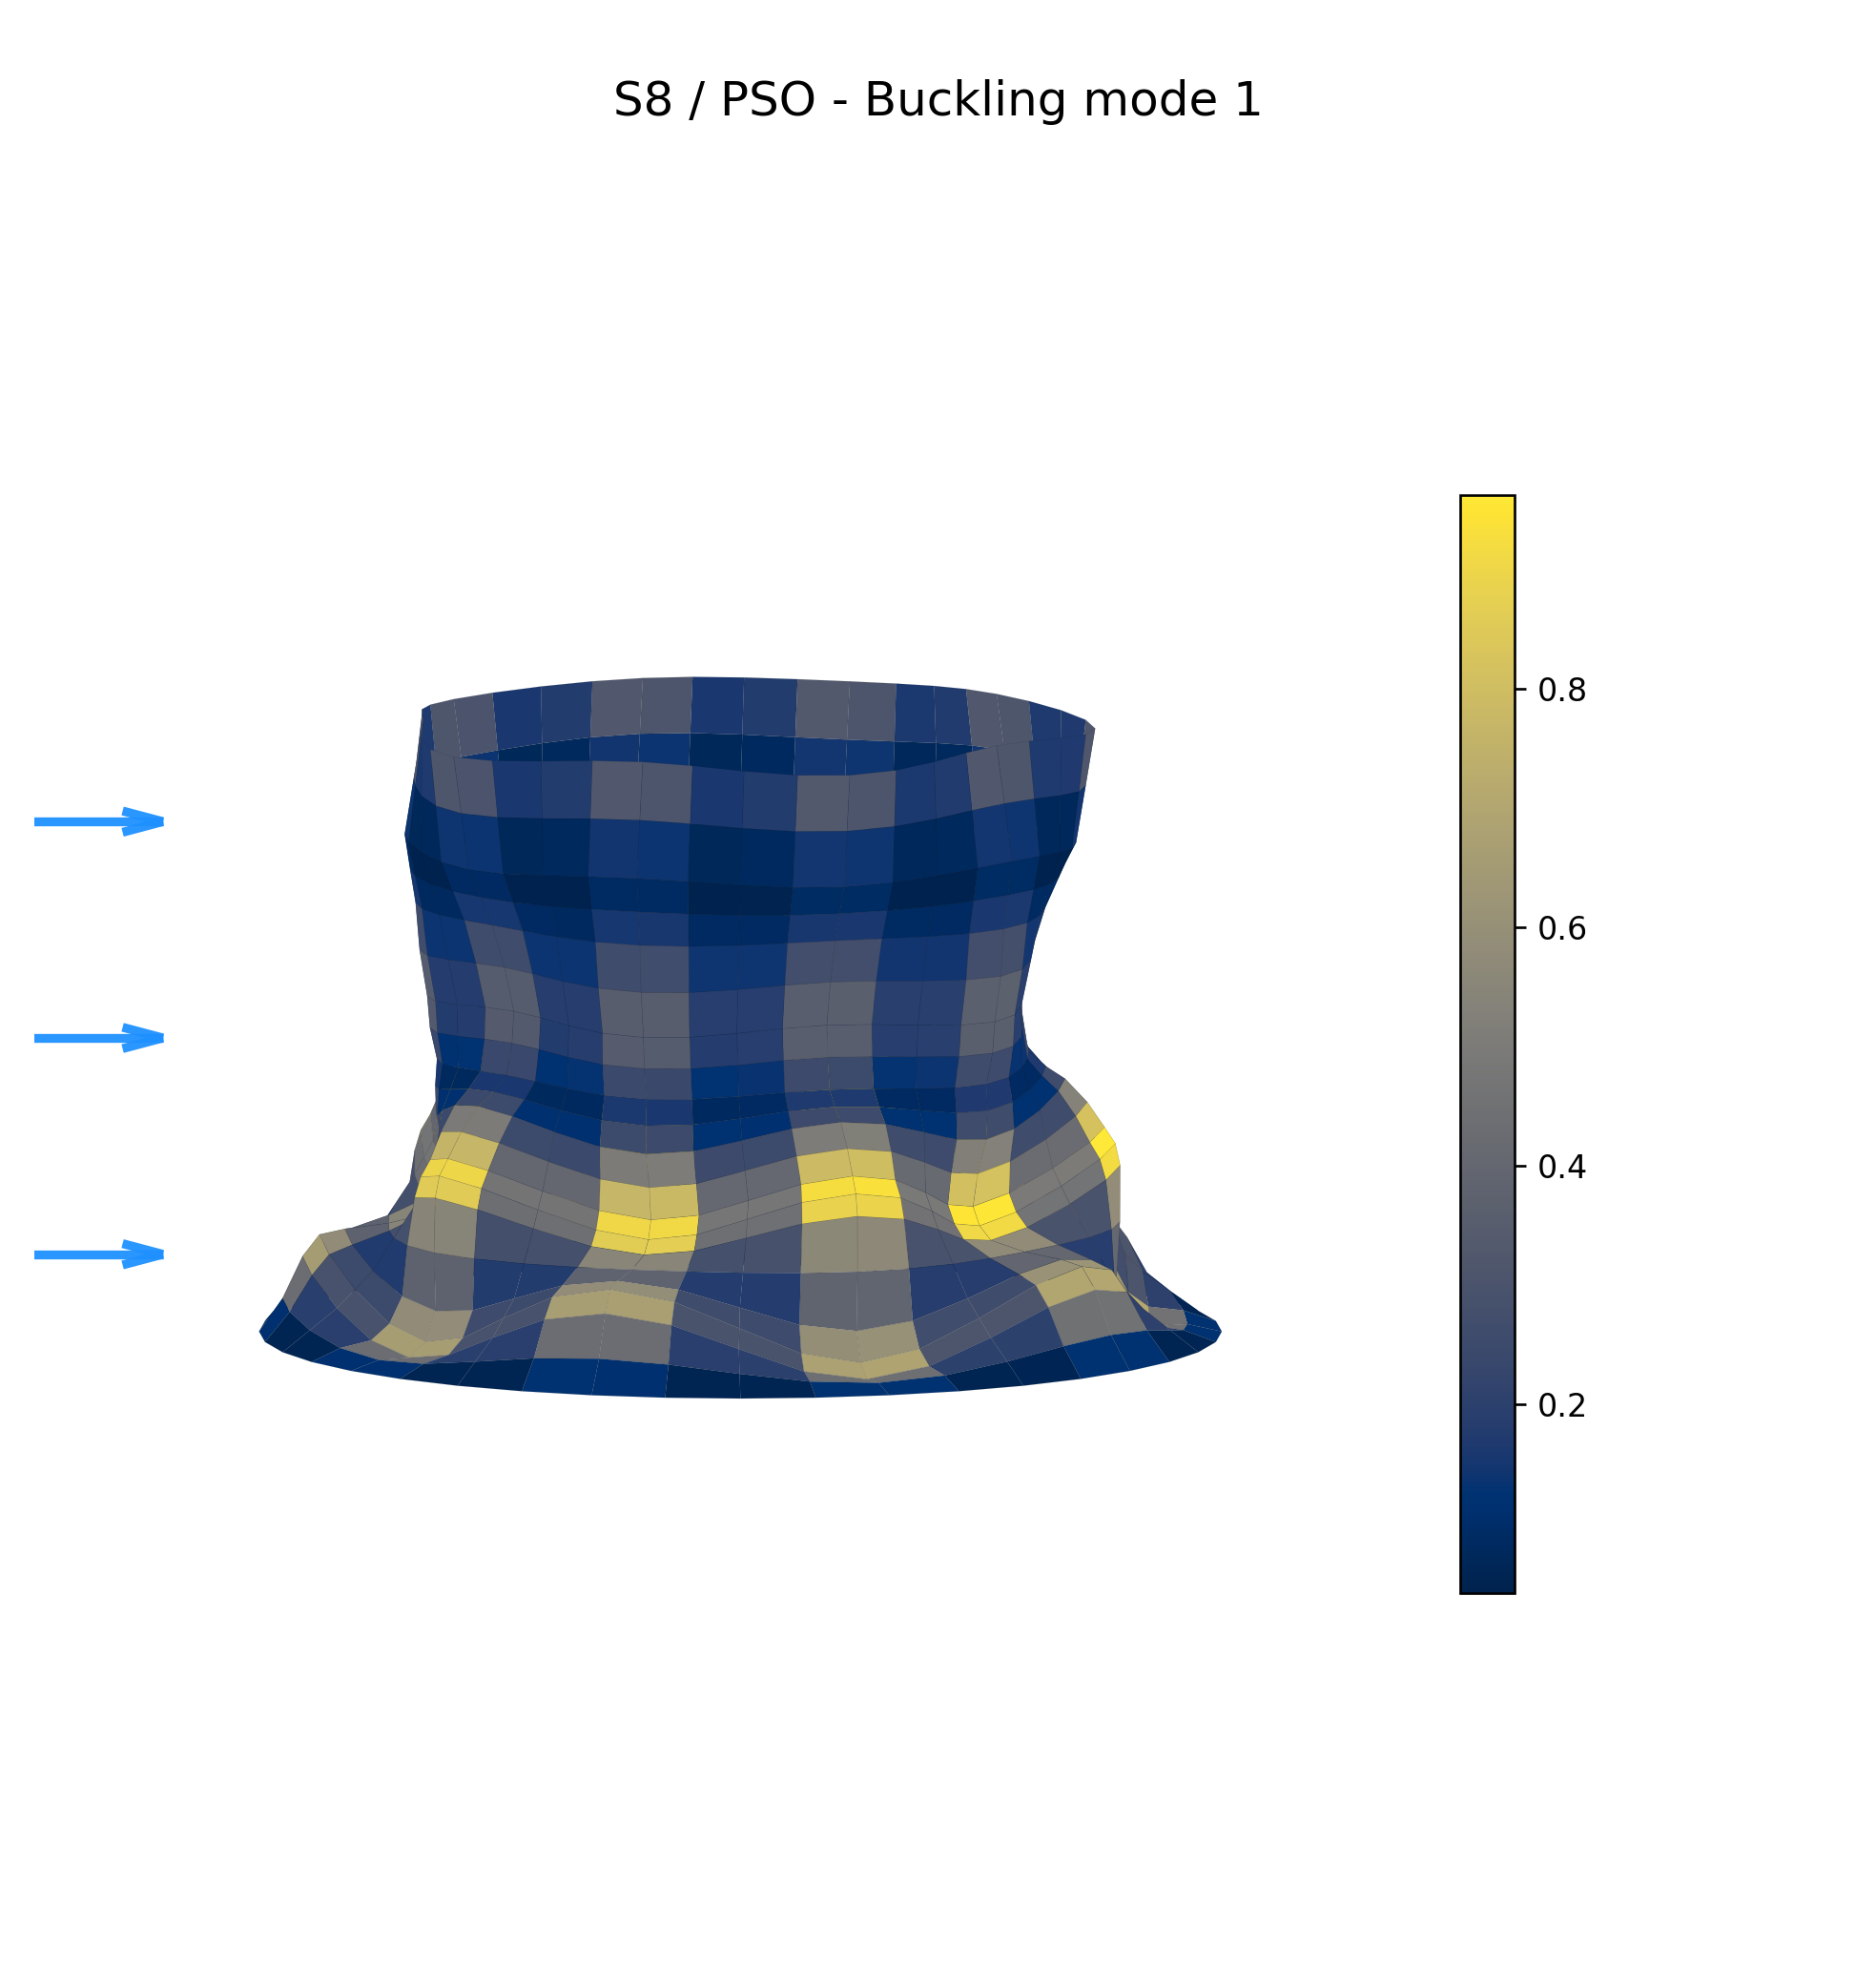
\includegraphics[width=\textwidth]{../results/figures/task7_s8_pso_buckling_mode1.png}
\caption{S8 / PSO buckling}
\end{subfigure}
\caption{Combined visual fields}
\end{figure}


\subsection{S8 / SA}


\begin{figure}[H]
\centering
\begin{subfigure}{0.32\textwidth}
\centering
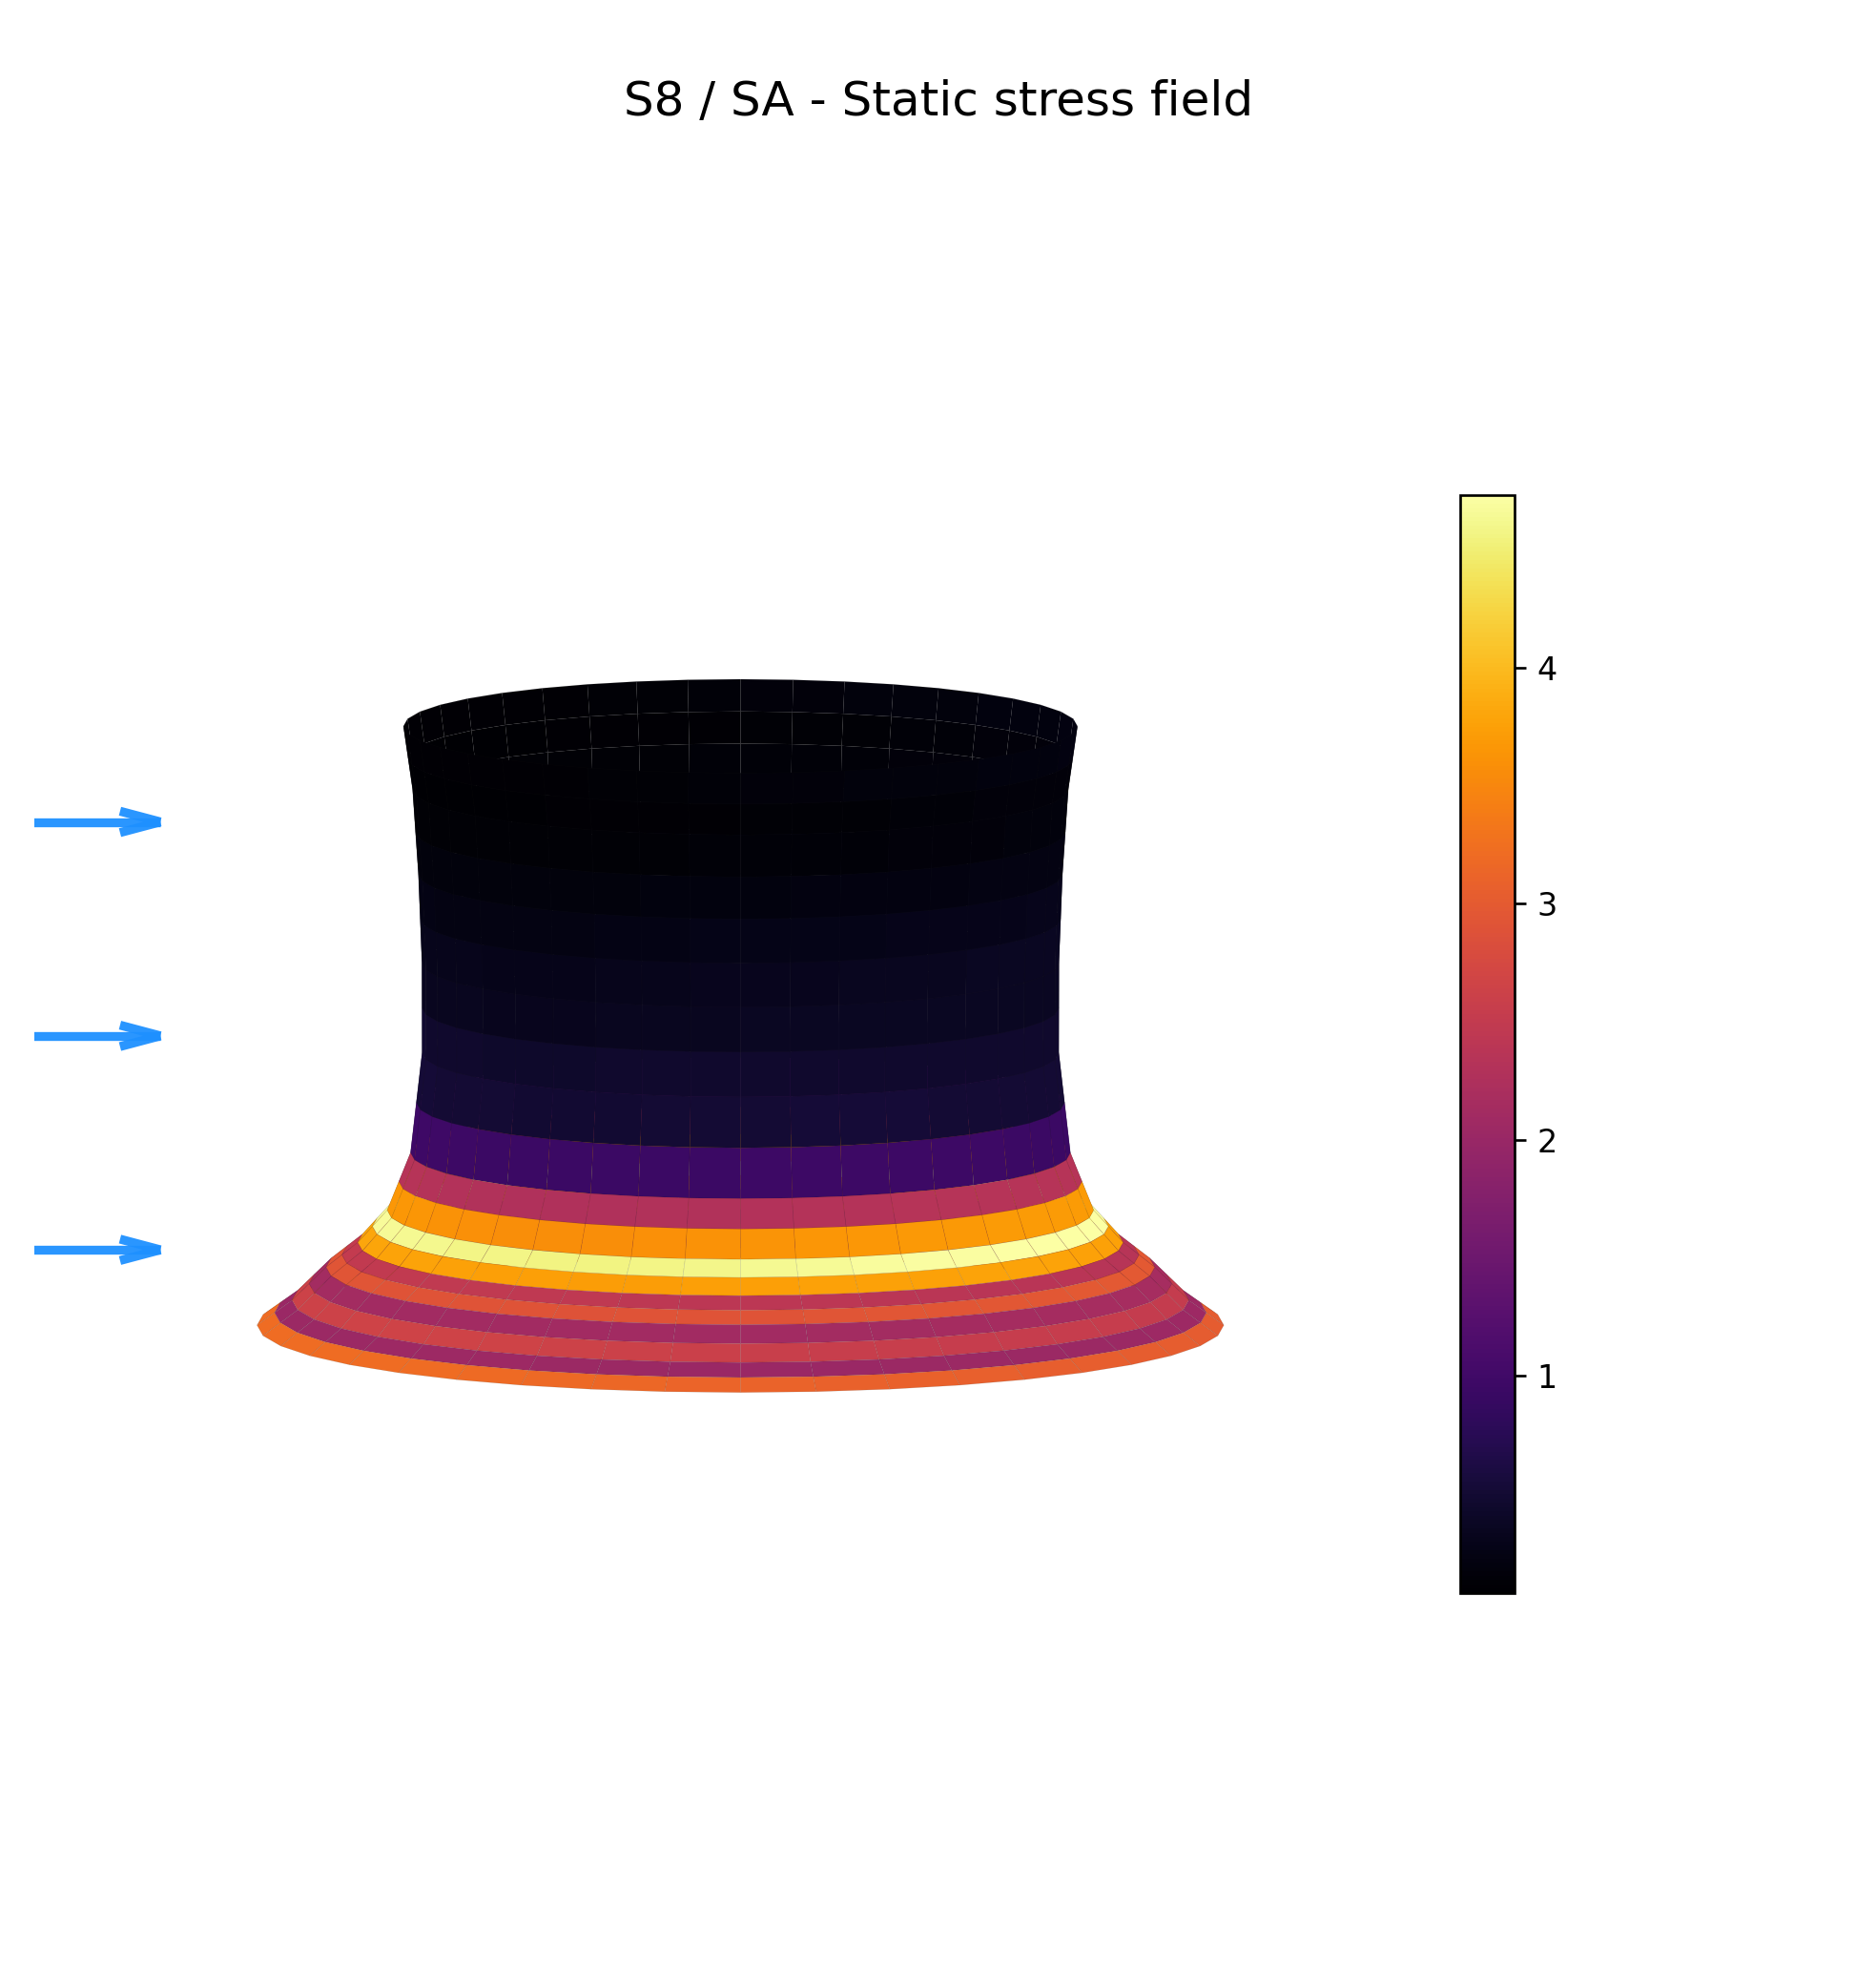
\includegraphics[width=\textwidth]{../results/figures/task7_s8_sa_stress.png}
\caption{S8 / SA stress}
\end{subfigure}\hfill
\begin{subfigure}{0.32\textwidth}
\centering
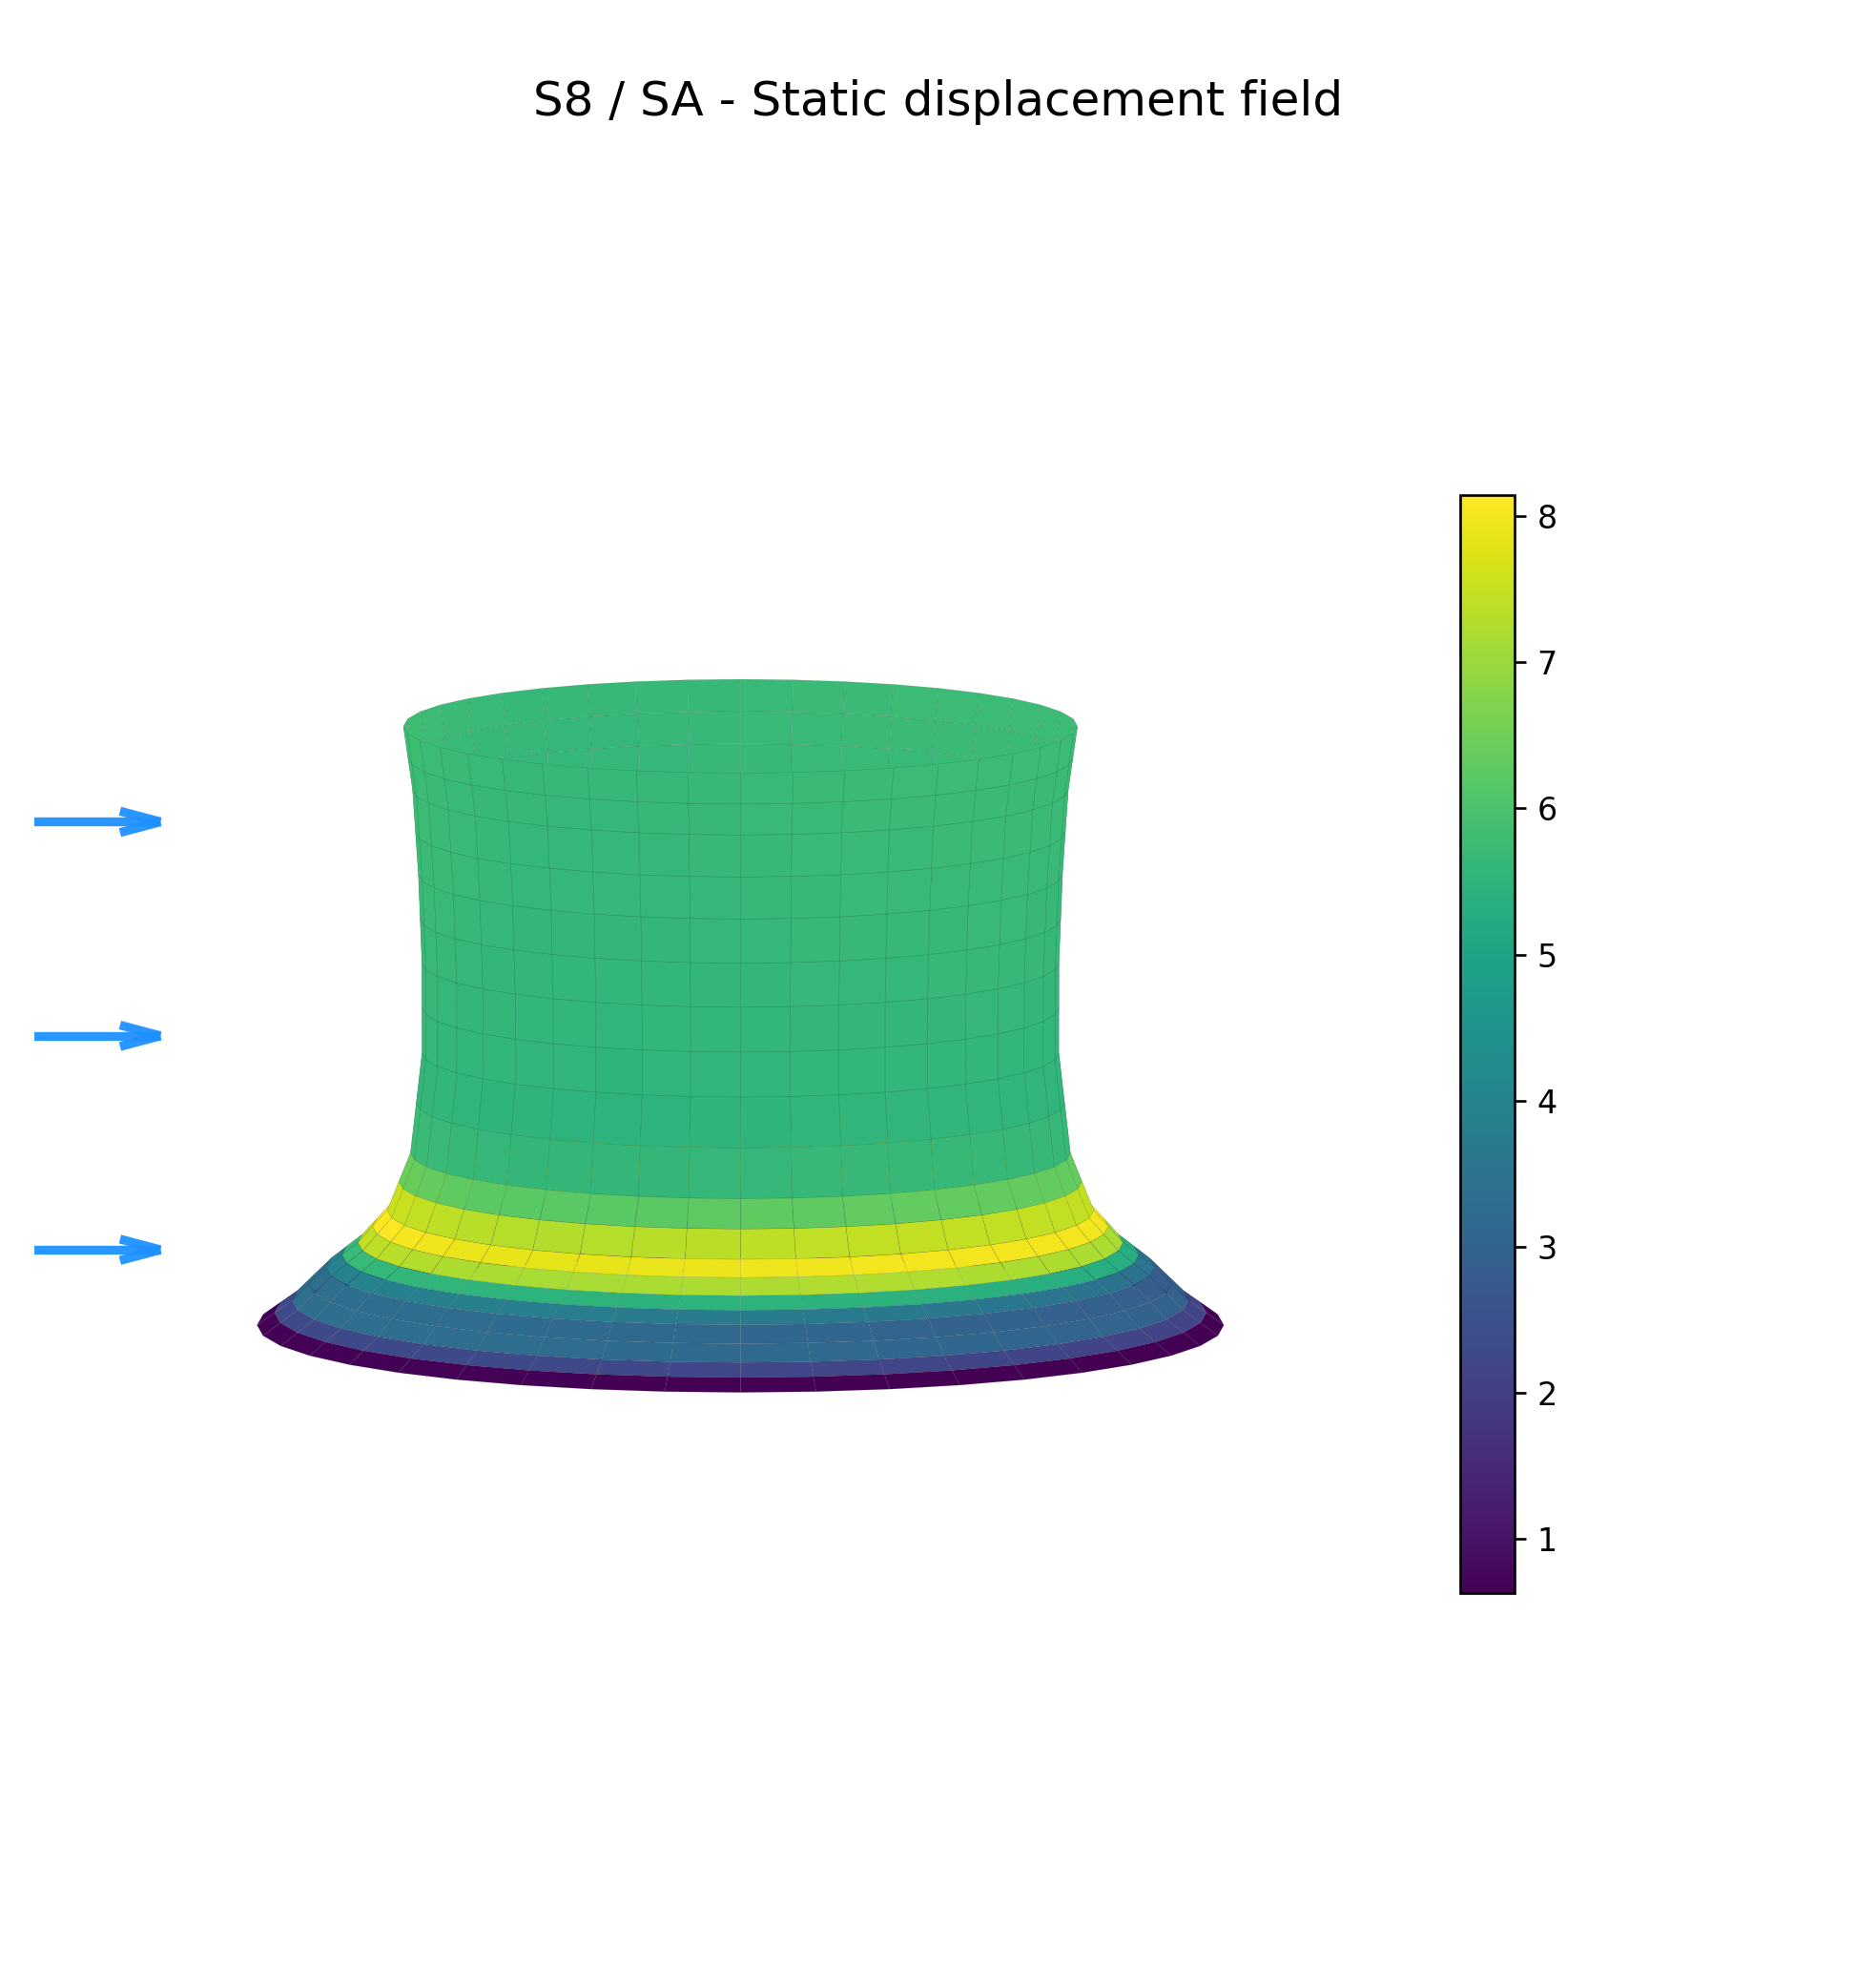
\includegraphics[width=\textwidth]{../results/figures/task7_s8_sa_displacement.png}
\caption{S8 / SA displacement}
\end{subfigure}\hfill
\begin{subfigure}{0.32\textwidth}
\centering
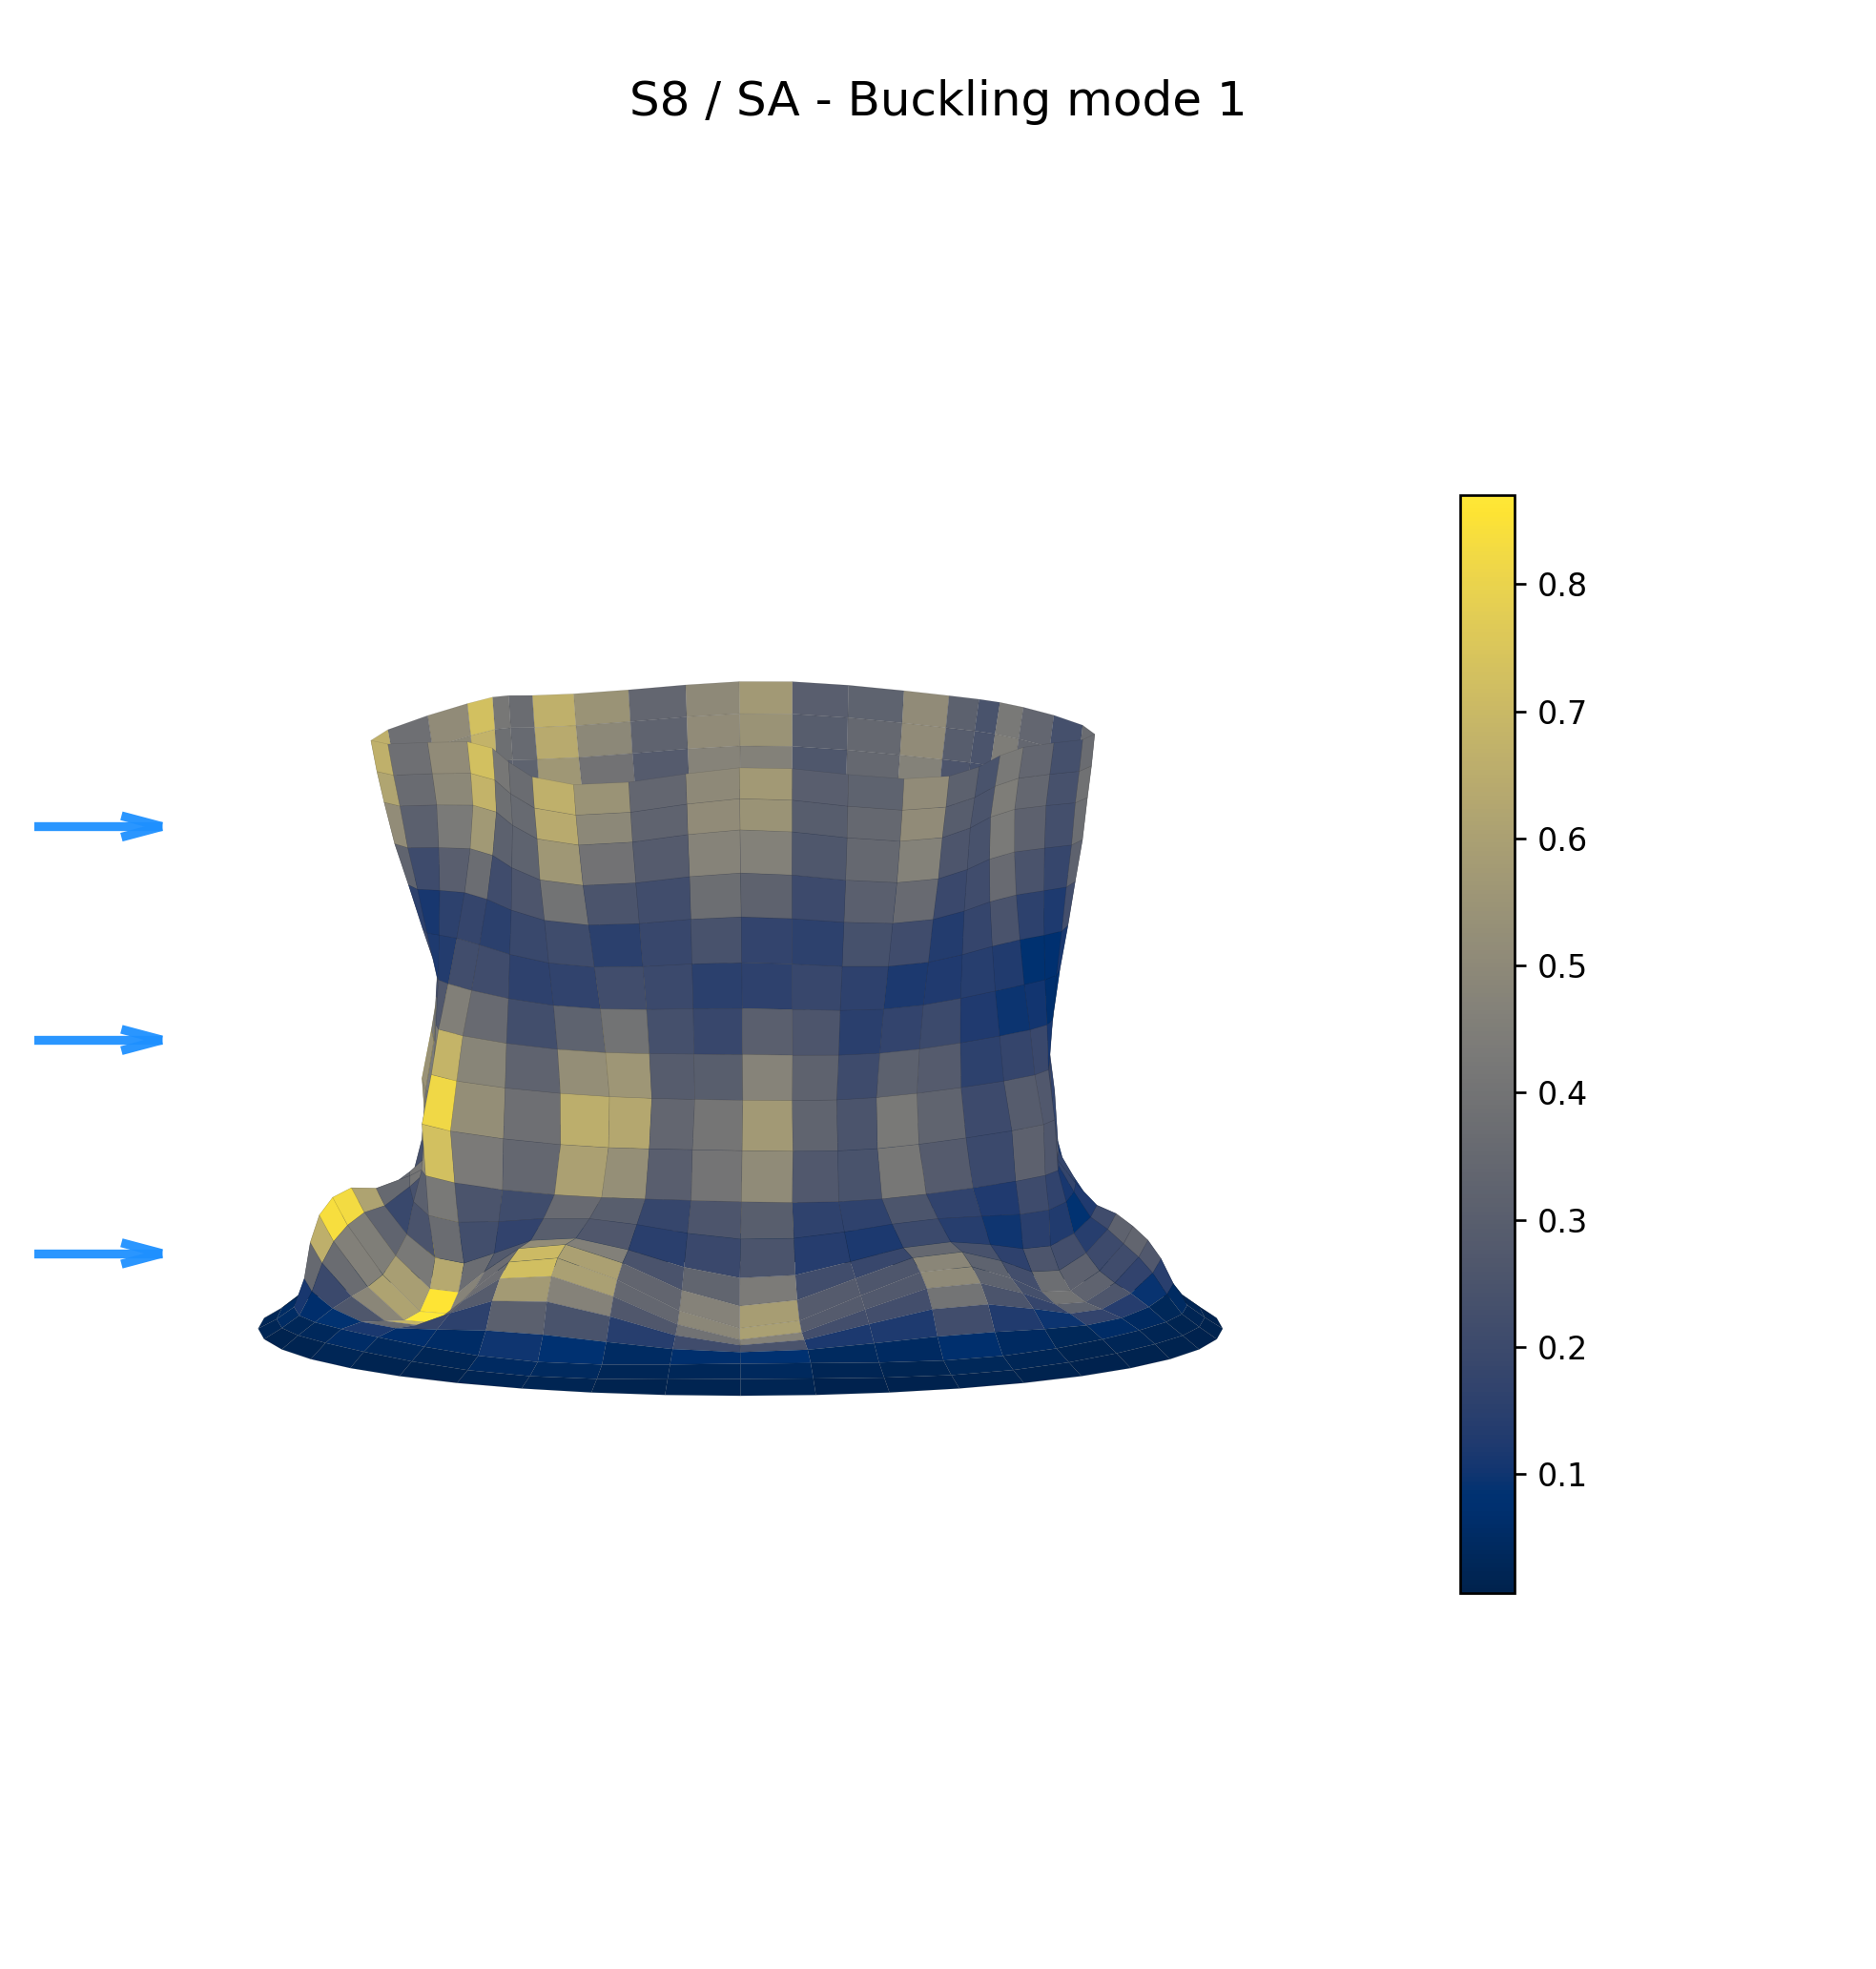
\includegraphics[width=\textwidth]{../results/figures/task7_s8_sa_buckling_mode1.png}
\caption{S8 / SA buckling}
\end{subfigure}
\caption{Combined visual fields}
\end{figure}
